\documentclass[9pt,letter,twoside,openright]{memoir}
\usepackage[svgnames,table]{xcolor}
\usepackage{circuitikz}
\usepackage{xparse}
%\usepackage{minibox}
\usepackage{longtable}
\usepackage{amsmath,pgfplots}
\usepackage[shortlabels]{enumitem}
%\usepackage{tkz-euclide}
%\usetkzobj{all}
\usepackage{tikz}
\usetikzlibrary{decorations.fractals,calc}
\usepackage{amssymb}
\usepackage{etoolbox}
\usepackage{cancel}
\usepackage{array}
\usepackage{graphicx}
\usepackage{framed}
\usepackage{tcolorbox}
\tcbuselibrary{breakable,skins,xparse}
\usepackage{marginnote}
%\usepackage{verbatim}
\usepackage[style=2]{mdframed}
\usepackage[top=0.75in, bottom=0.75in, inner=0.75in, outer=2.5in, marginparwidth=1.75in, marginparsep=0.25in]{geometry}
\usepackage{titlesec}
\usepackage[official]{eurosym}
%\usepackage[Bjornstrup]{fncychap}

\usepackage{changepage}
\usepackage[T1]{fontenc}
\usepackage{lmodern}
%\usepackage{url}
\usepackage{comment}
\ifpdf
  \usepackage{pdfcolmk}
\fi
\usepackage{graphicx}
\usepackage[hidelinks]{hyperref}
%\usepackage[outline]{contour}
\usepackage{pifont}
\ifxetex
  \usepackage{fontspec}
\fi

\strictpagecheck
\addtocontents{toc}{\protect\thispagestyle{empty}}

%%%%Author Name in Table of Contents---------
\makeatletter
\let\@nodottedtocline\@dottedtocline
\patchcmd{\@nodottedtocline}{\hbox{.}}{\hbox{}}{}{}
\patchcmd{\@nodottedtocline}{\normalcolor #5}{\normalcolor}{}{}
\newcommand*\l@sectionsubtitle{\@nodottedtocline{1}{0em}{1.5em}}
\makeatother

\def\sectionsubtitle#1{%
    \addcontentsline{toc}{sectionsubtitle}{\protect\numberline{}\textit{#1}}%
}
%%%%------------------------------------------

%%%%Define Gaussian Plot for Stats Chapter
\pgfmathdeclarefunction{gauss}{2}{%
  \pgfmathparse{1/(#2*sqrt(2*pi))*exp(-((x-#1)^2)/(2*#2^2))}%
}
%%%%End Define Gaussian Plot

%%%%Drawing Fractal
\newcommand{\bedknobsthree}[1]{
    %\begin{center}
        \tikz [
            decoration = #1
        ] \draw decorate{ decorate{ decorate{ (0, 0) -- (0.35\linewidth, 0) }}};
    %\end{center}
}
%%%%Drawing Fractal

%%%%Begin Header Format
\nouppercaseheads
\copypagestyle{doc}{companion}
\makeevenhead{doc}{\textbf{\Large \thepage} \hspace{0.1in} \textbf{CHAPTER \thechapter} \hspace{0.1in} \leftmark}{}{}
\makeoddhead{doc}{}{}{SECTION \rightmark \hspace{0.1in} \textbf{\Large \thepage}}
\makeevenfoot{doc}{}{}{}
\makeoddfoot{doc}{}{}{}
\makeheadrule{doc}{\textwidth}{0pt} %Uncomment to remove headrule

\copypagestyle{chapter}{doc}
\makeevenhead{chapter}{}{}{}
\makeoddhead{chapter}{}{}{}
\makeevenfoot{chapter}{\textbf{\Large \thepage}}{}{}
\makeoddfoot{chapter}{\hfill}{\hfill}{\textbf{\Large \thepage}}
\makeheadrule{chapter}{\textwidth}{0pt} %Uncomment to remove headrule

\copypagestyle{exercise}{doc}
\makeevenfoot{exercise}{
\begin{tikzpicture}[overlay,remember picture]
      \fill [color=blue!60!black]
        (current page.north west)
        rectangle
        ($ (current page.south west) + (1cm,0cm) $);
\end{tikzpicture}
}{}{}
\makeoddfoot{exercise}{\hfill}{\hfill}{
\begin{tikzpicture}[overlay,remember picture]
      \fill [color=blue!60!black]
        (current page.north east)
        rectangle
        ($ (current page.south east) - (1cm,0cm) $);
\end{tikzpicture}
}

\setsecheadstyle{\Large\scshape\raggedright\bfseries\color{blue!30!black}}
\setsubsecheadstyle{\large\scshape\raggedright}
\setsubsubsecheadstyle{\normalsize\scshape\raggedright}
\setbeforesecskip{-1.5ex plus -.5ex minus -.2ex}
\setaftersecskip{1.3ex plus .2ex}
\setbeforesubsecskip{-1.25ex plus -.5ex minus -.2ex}
\setaftersubsecskip{1ex plus .2ex}
%%%%End Header Format

%%%%Begin Chapter Header Format
\usepackage{color,calc}
\newsavebox{\ChpNumBox}
\definecolor{ChapBlue}{rgb}{0.2,0.6,1}
\makeatletter
%\newcommand*{\thickhrulefill}{%
%\leavevmode\leaders\hrule height 1\p@ \hfill \kern \z@}
\newcommand*{\thickhrulefill}{\rule{1.0\textwidth}{5pt}}
\newcommand*\BuildChpNum[2]{%
\begin{tabular}[t]{@{}c@{}}
\makebox[0pt][c]{#1\strut} \\[.5ex]
\colorbox{ChapBlue}{%
\rule[-10em]{0pt}{0pt}%
\rule{1ex}{0pt}\color{black}#2\strut
\rule{1ex}{0pt}}%
\end{tabular}}
\makechapterstyle{BlueBox}{%
\renewcommand{\chapnamefont}{\large\scshape}
\renewcommand{\chapnumfont}{\Huge\bfseries}
\renewcommand{\chaptitlefont}{\raggedright\Huge\bfseries}
\setlength{\beforechapskip}{20pt}
\setlength{\midchapskip}{26pt}
\setlength{\afterchapskip}{40pt}
\renewcommand{\printchaptername}{}
\renewcommand{\chapternamenum}{}
\renewcommand{\printchapternum}{%
\sbox{\ChpNumBox}{%
\BuildChpNum{\chapnamefont\@chapapp}%
{\chapnumfont\thechapter}}}
\renewcommand{\printchapternonum}{%
\sbox{\ChpNumBox}{%
\BuildChpNum{\chapnamefont\vphantom{\@chapapp}}%
{\chapnumfont\hphantom{\thechapter}}}}
\renewcommand{\afterchapternum}{}
\renewcommand{\printchaptertitle}[1]{%
\usebox{\ChpNumBox}\hfill
\parbox[t]{\hsize-\wd\ChpNumBox-1em}{%
\vspace{\midchapskip}%
\thickhrulefill\par
\chaptitlefont ##1\par}}%
}
\chapterstyle{BlueBox}
%%%%End Chapter Header Format

%%%%Begin Title Page Definition
\newlength{\drop}
\newcommand*{\FSfont}[1]{%
  \fontencoding{T1}\fontfamily{#1}\selectfont}
\renewcommand*{\FSfont}[1]{}%    kills special font selections

\newcommand*{\rotrt}[1]{\rotatebox{90}{#1}}
\newcommand*{\rotlft}[1]{\rotatebox{-90}{#1}}
\newcommand*{\topb}{%
  \resizebox*{\unitlength}{\baselineskip}{\rotrt{$\}$}}}
\newcommand*{\botb}{%
  \resizebox*{\unitlength}{\baselineskip}{\rotlft{$\}$}}}
\newcommand*{\titleBC}{\begingroup
\begin{center}
\settowidth{\unitlength}{\textit{\Large COMMON APPLICATIONS OF MATHEMATICS}} 
{\color{LightGoldenrod}\topb} \\[\baselineskip]
\textcolor{Sienna}{\textit{\HUGE Versatile Mathematics}} \\[\baselineskip]
{\color{RosyBrown}\Large COMMON MATHEMATICAL APPLICATIONS} \\
{\color{LightGoldenrod}\botb}
\end{center}
\vfill
\begin{center}
{\LARGE\textbf{by FCC Math Faculty}}\\
\vfill

\includegraphics[height=0.5in]{Banner.jpg}\\
2015
\end{center}
\endgroup}
%%%%End Title Page Definition

%Makes labels on axes smaller
\pgfplotsset{
    every axis/.append style={font=\tiny},  
}
%

%%%%Begin Procedure Definition
\newtcolorbox{proc}[1]{enhanced,colback=green!15!white,colframe=green!40!white!50!black,drop fuzzy shadow, toprule=5pt,bottomrule=0mm,rightrule=0mm,leftrule=0mm,fonttitle=\large,title={\fontfamily{fvs}\selectfont \textbf{#1}},sharp corners=all}
%%%%End Procedure Definition

\def\fra#1#2{\vskip #2\noindent\textcolor{black!60!red}{\rule{\textwidth}{2pt}}}

%%%%Begin Try It Definition
\renewcommand{\pfbreakdisplay}{%
\ding{167}\quad\ding{167}\quad\ding{167}}

\newenvironment{try}[1][http://www.frederick.edu/]
{
\begin{tcolorbox}[enhanced,beforeafter skip=10pt,breakable,colframe=yellow!10,colback=yellow!10,drop lifted shadow,sharp corners=all]
\marginnote{\href{#1}{\fontfamily{fvs}\selectfont \Large\color{black!70!orange}\textbf{TRY IT}}}
}
{ \end{tcolorbox}}
%%%%End Try It Definition

%%%%Begin Formula Definition
\newenvironment{formula}[1]
{\begin{tcolorbox}[beforeafter skip=10pt,colframe=black!10,colback=blue!70!cyan!20!white,opacityfill=0.5,toprule=0mm,bottomrule=0mm,rightrule=0mm,leftrule=0mm,sharp corners=all]

{\fontfamily{fvs}\selectfont \Large\bfseries #1}\\

}
{\end{tcolorbox}}
%%%%End Formula Definition

%%%%Counter for examples; reset for each chapter/section?
\newcounter{ExampleCounter}
\setcounter{ExampleCounter}{1}

%%%%Begin Example Definition
\begin{comment}
\newenvironment{example}[2][https://dl.dropboxusercontent.com/u/28928849/Webpages/MathInSocietyVideos2.htm]
{
\marginnote{\href{#1}{\fontfamily{fvs}\selectfont \Large\color{black!70!blue!80!cyan}\uppercase{\bfseries\centering EXAMPLE \theExampleCounter}
}}[9.2mm]
\begin{tcolorbox}[check odd page,toggle left and right,
beforeafter skip=10pt,breakable,bottomrule at break=0mm,toprule at break=0mm,colframe=black!50!blue!50!cyan,colback=white,toprule=0mm,rightrule=0mm,sharp corners=all] 
{%\renewcommand*\sfdefault{iwona}
\checkoddpage
\ifoddpage{
\hfill {\href{#1}{\fontfamily{fvs}\selectfont \Large\color{black!70!blue!80!cyan}\uppercase{\bfseries #2}}}}\\
 \else{
{\href{#1}{\fontfamily{fvs}\selectfont \Large\color{black!70!blue!80!cyan}\uppercase{\bfseries #2}}}}\\
\fi
\end{comment}

\colorlet{colexam}{black!50!blue!50!cyan}
\newenvironment{example}[2][https://dl.dropboxusercontent.com/u/28928849/Webpages/MathInSocietyVideos2.htm]
{
\begin{tcolorbox}[empty,
breakable,
if odd page*={overlay unbroken={\coordinate (X) at ([yshift=-10pt]frame.north west); \coordinate (Y) at (frame.south west); \coordinate (Z) at (frame.south east);
\draw[black!50!blue!50!cyan,line width=2pt]
(X)--(Y)--(Z); },
overlay first={\coordinate (X) at ([yshift=-10pt]frame.north west); \coordinate (Y) at (frame.south west);
\draw[black!50!blue!50!cyan,line width=2pt]
(X)--(Y); },
overlay middle={\coordinate (X) at ([yshift=-10pt]frame.north west); \coordinate (Y) at (frame.south west);
\draw[black!50!blue!50!cyan,line width=2pt]
(X)--(Y); },
overlay last={\coordinate (X) at ([yshift=-10pt]frame.north west); \coordinate (Y) at (frame.south west); \coordinate (Z) at (frame.south east);
\draw[black!50!blue!50!cyan,line width=2pt]
(X)--(Y)--(Z); }}{overlay unbroken={\coordinate (X) at ([yshift=-10pt]frame.north east); \coordinate (Y) at (frame.south east); \coordinate (Z) at (frame.south west);
\draw[black!50!blue!50!cyan,line width=2pt]
(X)--(Y)--(Z); },
overlay first={\coordinate (X) at ([yshift=-10pt]frame.north east); \coordinate (Y) at (frame.south east);
\draw[black!50!blue!50!cyan,line width=2pt]
(X)--(Y); },
overlay middle={\coordinate (X) at ([yshift=-10pt]frame.north east); \coordinate (Y) at (frame.south east);
\draw[black!50!blue!50!cyan,line width=2pt]
(X)--(Y); },
overlay last={\coordinate (X) at ([yshift=-10pt]frame.north east); \coordinate (Y) at (frame.south east); \coordinate (Z) at (frame.south west);
\draw[black!50!blue!50!cyan,line width=2pt]
(X)--(Y)--(Z); }}] 
{%\renewcommand*\sfdefault{iwona}
\checkoddpage
\ifoddpage{
\hfill {\href{#1}{\fontfamily{fvs}\selectfont \Large\color{black!70!blue!80!cyan}\uppercase{\bfseries #2}\marginnote{\href{#1}{\fontfamily{fvs}\selectfont \Large\color{black!70!blue!80!cyan}\uppercase{\bfseries\centering EXAMPLE \theExampleCounter}
}}}}}\\
 \else{
{\href{#1}{\fontfamily{fvs}\selectfont \Large\color{black!70!blue!80!cyan}\uppercase{\bfseries #2}\marginnote{\href{#1}{\fontfamily{fvs}\selectfont \Large\color{black!70!blue!80!cyan}\uppercase{\bfseries\centering EXAMPLE \theExampleCounter}
}}}}}\\
\fi
%\renewcommand*\sfdefault{cmr}
}

%\Large\color{black!70!blue!80!cyan}\scshape #2}\\

}
{ \end{tcolorbox} \stepcounter{ExampleCounter}}

\newcommand{\sol}{\marginnote{\bfseries Solution}}
%%%%End Example Definition

%%%%Begin Section Definition
\newcounter{SectionNo}[chapter]

\DeclareDocumentCommand \section { m }
{
\phantomsection
\stepcounter{section}
\addcontentsline{toc}{section}{\thesection\ #1}
\sectionmark{#1}

\checkoddpage
\ifoddpage{\begin{adjustwidth}{0in}{-1.75in}
\stepcounter{SectionNo}
	
	\tcbset{enhanced,colback=brown!70!white,colframe=brown!75!black}
	\begin{tcolorbox}[toprule=3mm,sharp corners = all]
	{\fontfamily{fvs}\selectfont \huge\bfseries\color{white} SECTION \thechapter .\theSectionNo} \ {\fontfamily{fvs}\selectfont \LARGE\bfseries\color{black!80} #1}
	\end{tcolorbox}
	
 \end{adjustwidth}}
\else{\begin{adjustwidth}{-1.75in}{0in}
\stepcounter{SectionNo}
	
	\tcbset{enhanced,colback=brown!70!white,colframe=brown!75!black}
	\begin{tcolorbox}[toprule=3mm,sharp corners = all]
	{\fontfamily{fvs}\selectfont \huge\bfseries\color{white} SECTION \thechapter .\theSectionNo} \ {\fontfamily{fvs}\selectfont \LARGE\bfseries\color{black!80} #1}
	\end{tcolorbox}
	
 \end{adjustwidth}}
\fi
}

\DeclareDocumentCommand \subsection { m }
{
\vspace{0.2in}
{\fontfamily{fvs}\selectfont \LARGE\color{brown!65!black} \textbf{#1}}
\vspace{0.1in}\\
}
%%%%End Section Definition

%%%%Begin Example 2.0 Definition
\newcounter{example}[SectionNo]

\DeclareDocumentCommand \examplet { O{www.google.com} +m O{www.frederick.edu} +m }
{
\stepcounter{example}
\checkoddpage
\ifoddpage{\begin{adjustwidth}{0in}{-1.75in}
\begin{tcolorbox}[enhanced,breakable,drop lifted shadow,sharp corners=all,sidebyside,sidebyside align=top seam,title=\href{#1}{{\Large\bfseries\color{blue!40!black}EXAMPLE \theexample}} \hfill \href{#3}{{\Large\bfseries\color{green!40!black} TRY IT}},colframe=white,bottomrule=0mm,righthand width=2in,bicolor,colback=brown!15!white,colbacklower=yellow!10] #2 \tcblower #4
\end{tcolorbox}
\end{adjustwidth}}
\else{
\begin{adjustwidth}{-1.75in}{0in}
\begin{tcolorbox}[enhanced,breakable,drop lifted shadow,sharp corners=all,sidebyside,sidebyside align=top seam,title=\href{#1}{{\Large\bfseries\color{blue!40!black}EXAMPLE \theexample}} \hfill \href{#3}{{\Large\bfseries\color{green!40!black} TRY IT}},colframe=white,bottomrule=0mm,righthand width=2in,bicolor,colback=brown!15!white,colbacklower=yellow!10] #2 \tcblower #4
\end{tcolorbox}
\end{adjustwidth}}
\fi
}

\begin{comment}
\DeclareDocumentCommand \example { O{www.google.com} +m }
{
\stepcounter{example}
\checkoddpage
\ifoddpage{\begin{adjustwidth}{0in}{-1.75in}
\begin{tcolorbox}[enhanced,breakable,drop lifted shadow,sharp corners=all,title=\href{#1}{{\Large\bfseries\color{blue!40!black}EXAMPLE \theexample}},colframe=white,bottomrule=0mm,colback=brown!15!white] #2
\end{tcolorbox}
\end{adjustwidth}}
\else{
\begin{adjustwidth}{-1.75in}{0in}
\begin{tcolorbox}[enhanced,breakable,drop lifted shadow,sharp corners=all,title=\href{#1}{{\Large\bfseries\color{blue!40!black}EXAMPLE \theexample}},colframe=white,bottomrule=0mm,colback=brown!15!white] #2
\end{tcolorbox}
\end{adjustwidth}}
\fi
}
\end{comment}
%%%%End Example 2.0 Definition

%%%%Begin Objectives Definition
%\newenvironment{objectives}
%{\begin{adjustwidth}{-1.5in}{0in}\begin{minipage}{0.5\textwidth}}
%{\end{minipage}\end{adjustwidth}}
\newenvironment{objectives}
{\marginnote{\begin{enumerate}}
{\end{enumerate}}}
%%%%End Objectives Definition

%%%%Begin Exercises Definition
\newcounter{ProblemNumber}

\newcommand\pone[1]{ %One exercise per line
  \noindent
  \begin{minipage}[t]{\textwidth}
  \vspace{0.1in}
    {\large\bfseries\theProblemNumber .} #1
  \vspace{0.1in}
  \end{minipage}
  \stepcounter{ProblemNumber}
}

\newcommand\ptwo[1]{ %Two exercises per line
  \noindent
  \begin{minipage}[t]{0.48\textwidth}
  \vspace{0.1in}
    {\large\bfseries\theProblemNumber .} #1
  \vspace{0.1in}
  \end{minipage}
  \stepcounter{ProblemNumber}
}

\newcommand\pthree[1]{ %Three exercises per line
  \noindent
  \begin{minipage}[t]{0.31\textwidth}
  \vspace{0.1in}
    {\large\bfseries\theProblemNumber .} #1
  \vspace{0.1in}
  \end{minipage}
  \stepcounter{ProblemNumber}
}

\newcommand\pfour[1]{ %Four exercises per line
  \noindent
  \begin{minipage}{0.228\textwidth}
  \vspace{0.15in}
    {\large\bfseries\theProblemNumber .} #1
  \vspace{0.15in}
  \end{minipage}
  \stepcounter{ProblemNumber}
}

\newenvironment{exercises}
{ 
	\newgeometry{margin=0.75in}	
	\pagestyle{exercise}
	\setcounter{ProblemNumber}{1}
	\noindent{\href{https://www.myopenmath.com/index.php}{\Huge\bfseries\color{blue!60!black} Exercises \thesection}}\\
	\checkoddpage
	\ifoddpage{{\color{blue!60!black} \rule{1.1\textwidth}{3pt}}} 
	\else{\begin{adjustwidth}{-0.8in}{0in}{\color{blue!60!black} \rule{1.1\textwidth}{3pt}}\end{adjustwidth}} 
	\fi
	%{\color{blue!60!black} \rule{1.1\textwidth}{3pt}}
	

%\begin{comment}
%\tikz[remember picture,overlay] {%
%\draw [blue!60!black,line width=10mm]
%(current page.south east)
%rectangle
%(current page.north east)
%;}
%\end{comment}


}
{ \setcounter{ProblemNumber}{1}
  \restoregeometry
  \pagestyle{doc} }
%%%%End Exercises Definition

%%%%Begin Chapter Summary Definition
\newenvironment{summary}
{ 
	\newgeometry{margin=0.75in}	
	\pagestyle{exercise}
	\setcounter{ProblemNumber}{1}
	\noindent{\href{https://www.myopenmath.com/index.php}{\Huge\bfseries\color{blue!60!black} Exercises \thesection}}\\
	{\color{blue!60!black} \rule{1.1\textwidth}{3pt}}
	

%\begin{comment}
%\tikz[remember picture,overlay] {%
%\draw [blue!60!black,line width=10mm]
%(current page.south east)
%rectangle
%(current page.north east)
%;}
%\end{comment}


}
{ \setcounter{ProblemNumber}{1}
  \restoregeometry
  \pagestyle{doc} }

%%%%End Chapter Summary Definition
\graphicspath{ {./Images/} }

\usetikzlibrary{arrows,decorations.markings,positioning}
\newcommand{\tikzmark}[2]{\tikz[overlay, remember picture] \node[inner sep=5pt, outer sep=5pt, anchor=base] (#1) {#2};}

\begin{document}
\frontmatter
\newgeometry{margin=1.25in}
\pagestyle{empty}
\titleBC
\frontmatter

\newgeometry{margin=0.75in}
\textbf{This text is licensed under a Creative Commons Attribution-Share Alike 3.0 United States License.}\\

To view a copy of this license, visit \href{http://creativecommons.org/licenses/by-sa/3.0/us/}{http://creativecommons.org/licenses/by-sa/3.0/us/} or send a letter to Creative Commons, 171 Second Street, Suite 300, San Francisco, California, 94105, USA\\

You are \textbf{free}:\\
\hspace*{0.25in} \textbf{to Share} -- to copy, distribute, display, and perform the work\\
\hspace*{0.25in} \textbf{to Remix} -- to make derivative works\\

Under the following conditions:\\
\hspace*{0.25in} \textbf{Attribution.}  You must attribute the work in the manner specified by the author or licensor (but not in any way that suggests that they endorse you or your use of the work).\\
\hspace*{0.25in} \textbf{Share Alike.}  If you alter, transform, or build upon this work, you may distribute the resulting work only under the same, similar, or a compatible license.\\

With the understanding of the following:\\
\hspace*{0.25in} \textbf{Waiver.}  Any of the above conditions can be waived if you get permission from the copyright holder.\\
\hspace*{0.25in} \textbf{Other Rights.}  In no way are any of the following rights affected by the license:
\begin{itemize}
\item Your fair dealing or fair use rights
\item Apart from the remix rights granted under this license, the authors' moral rights
\item Rights other persons may have either in the work itself or in how the work is used, such as publicity or privacy rights
\item Notice --- For any reuse or distribution, you must make clear to others the license terms of this work.  The best way to do this is with a link to the following web page: \href{http://creativecommons.org/licenses/by-sa/3.0/us/}{http://creativecommons.org/licenses/by-sa/3.0/us/}
\end{itemize}

\paragraph{Attributions} This book benefited tremendously from others who went before and freely shared their creative work.  The following is a short list of those whom we have to thank for their work and their generosity in contributing to the free and open sharing of knowledge.
\begin{itemize}
\item David Lippman, author of \textit{Math in Society}.  This book uses sections derived from his chapters on Finance, Growth Models, and Statistics.  He also administers MyOpenMath, the free online homework portal to which the problems in this text were added.
\item The developers of \href{onlinestatbook.com}{onlinestatbook.com}.
\item OpenStax College (their book \textit{Introductory Statistics} was used as a reference)

OpenStax College, \textit{Introductory Statistics}. OpenStax College. 19 September 2013. <http://cnx.org/content/col11562/latest/>
\item The authors of \href{https://www.openintro.org/stat/?stat_book=os}{OpenIntro Statistics}, which was also used as a reference.
\item The Saylor Foundation Statistics Textbook: http://www.saylor.org/site/textbooks/Introductory$\%$20Statistics.pdf
\end{itemize}

\paragraph{Thanks} The following is a short list of those whom we wish to thank for their help and support with this project.
\begin{itemize}
\item The President's office at Frederick Community College, for providing a grant to write the first chapters.
\item Gary Hull, who in his tenure as department chair gave us his full support and gave us the impetus to start the project, and generously shared his notes for MA 103.
\item The entire FCC math department, who provided untold support and encouragement, as well as aid in reviewing and editing the text.
\end{itemize}

%\restoregeometry





















%\clearpage
\setcounter{tocdepth}{1}
\newgeometry{margin=1.25in}
\tableofcontents*
\mainmatter
\restoregeometry
\pagestyle{doc}

\chapter{Financial Mathematics}
\begin{center}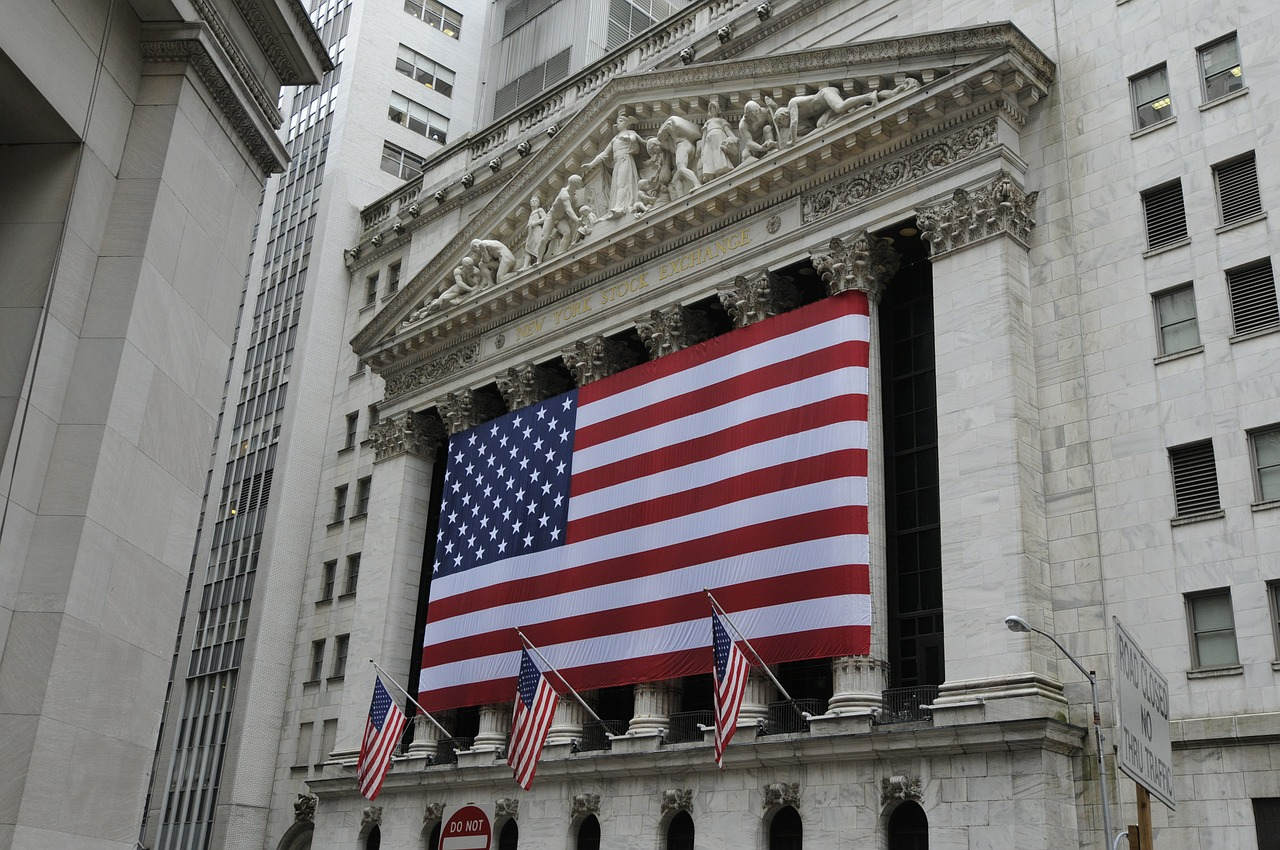
\includegraphics[width=\textwidth]{NYSE}\end{center}

In 2007, the U.S. mortgage bond market led to a financial crisis when thousands of subprime mortgages defaulted.  This led to a crash in the market that had a far-reaching impact on markets around the world, plunging the economy into a recession from 2007 to 2009.  Although the causes were complex and varied, at the root of the problem were these mortgages that were written in complicated terms that obscured the cost, and offered to borrowers who could not afford them.

The purpose of this chapter is to train you to be a savvy consumer.  No other area in this book will be as immediately and broadly applicable as this material on financial mathematics.  Here you'll begin to apply mathematical techniques to everyday financial management.  How much should you budget for a new car?  How is your federal income tax calculated?  When should you start saving for retirement?  The answers to these types of questions will be found in this chapter, as we investigate everything from sales tax to credit cards.  By understanding your personal finances, you can protect yourself and take control of your financial future.
\vfill
\pagebreak

\section{Percents and Their Applications}
Before we can dive into the mathematics of finance, we first need to review percentages, since we'll find that they are used to express concepts like interests rates.  Once we've gotten comfortable with percentages, we will use them for simple applications like sales tax calculations.

\subsection{Percents}
\marginnote{\textbf{Percent:} \\ number of hundredths}
A percentage is simply another way to represent a fraction or a decimal.  The word ``percent'' means ``per 100,'' or ``number of hundredths.''
\vspace{0.5in}

\begin{proc}{Percents, Fractions, and Decimals}
Since percent (\%) means ``number of hundredths,'' we can convert decimals to percents by multiplying by 100 (or moving the decimal point two places to the right).

We can convert fractions to percents the same way by first writing them as decimals.
\end{proc}
\vspace{0.5in}

\begin{example}[https://www.youtube.com/watch?v=UZHLvEmFrOk]{Converting to Percentages}
Convert each of the following to a percentage:\\

\begin{tabular}{l l l}
(a) $\dfrac{1}{4}$ & (b) $0.02$ & (c) $\dfrac{8}{3}$
\end{tabular}

\begin{center}
\marginnote{\bfseries Solution}
\begin{tabular}{l l l}
(a) $\dfrac{1}{4} = 0.25 = 25\%$ & (b) $0.02 = 2\%$ & (c) $\dfrac{8}{3} = 2.67 = 267\%$
\end{tabular}
\end{center}
\end{example}

\begin{try}[http://izzomath.com/103text/finance/example1.1/story.html]
Convert each of the following to a percentage:\\

\begin{tabular}{l l l}
(a) $\dfrac{3}{5}$ & (b) $0.7$ & (c) 2
\end{tabular}
\end{try}
\vspace{0.25in}

This process can be reversed to convert a percentage to a decimal.

To do so, simply remove the percent symbol and divide the percentage by 100 (i.e. move the decimal point two places to the left).
%\vfill
%\pagebreak

\begin{example}[https://www.youtube.com/watch?v=d770dB9RHIc]{Converting Percents to Decimals}
Convert the following percentages to decimals:\\

\begin{tabular}{l l l}
(a) 17\% & (b) 122\% & (c) 0.15\%
\end{tabular}

\begin{center}
\marginnote{\bfseries Solution}
\begin{tabular}{l l l}
(a) $17\% = 0.17$ & (b) $122\% = 1.22$ & (c) $0.15\% = 0.0015$
\end{tabular}
\end{center}
\end{example}
\vfill
\pagebreak

\subsection{Applied Percent Problems}
Of course, the real goal is to apply what we know about using percentages to applied problems.  These all boil down the statement ``A is P percent of B,'' written \[A = PB.\]  Remember, when translating a sentence into a mathematical expression, ``of'' gets replaced with multiplication.  Each of these applied percentage problems will give two of these pieces and leave the third unknown; our job will be to solve for the third piece.

\begin{example}[https://www.youtube.com/watch?v=8VSRt2PMqJI]{Coffee Survey}
The Frederick News Post did a poll of 1500 people, asking them the following question: ``Do you go to Starbucks at least 3 times a week?'' Of those 1500 polled, 58\% said ``yes.''  How many people replied yes to the survey?\\

\marginnote{\bfseries Solution}
Remember that the keyword ``of'' in a word problem usually refers to multiplication, so ``58\% \textbf{of} 1500'' translates to ``58\% $\cdot$ 1500,'' but to do the multiplication, we need to write the percentage as a decimal:
\[58\% \cdot 1500 = 0.58 \cdot 1500 = 870\]

Thus, 870 people responded ``yes'' to the survey.
\end{example}

\begin{try}[http://izzomath.com/103text/finance/example1.4/story.html]
If there are 6,233 students enrolled this semester, and 59\% of those are women, how many women are attending the college this semester?
\end{try}

From the equation $A=PB$ we can solve for the percentage $P$ by dividing both sides by $B$.  This gives us the form $P=\dfrac{A}{B}$, which is useful when we want to find the percentage.

\begin{example}[https://www.youtube.com/watch?v=C8SnqyhsVeo]{Dog People}
\marginnote{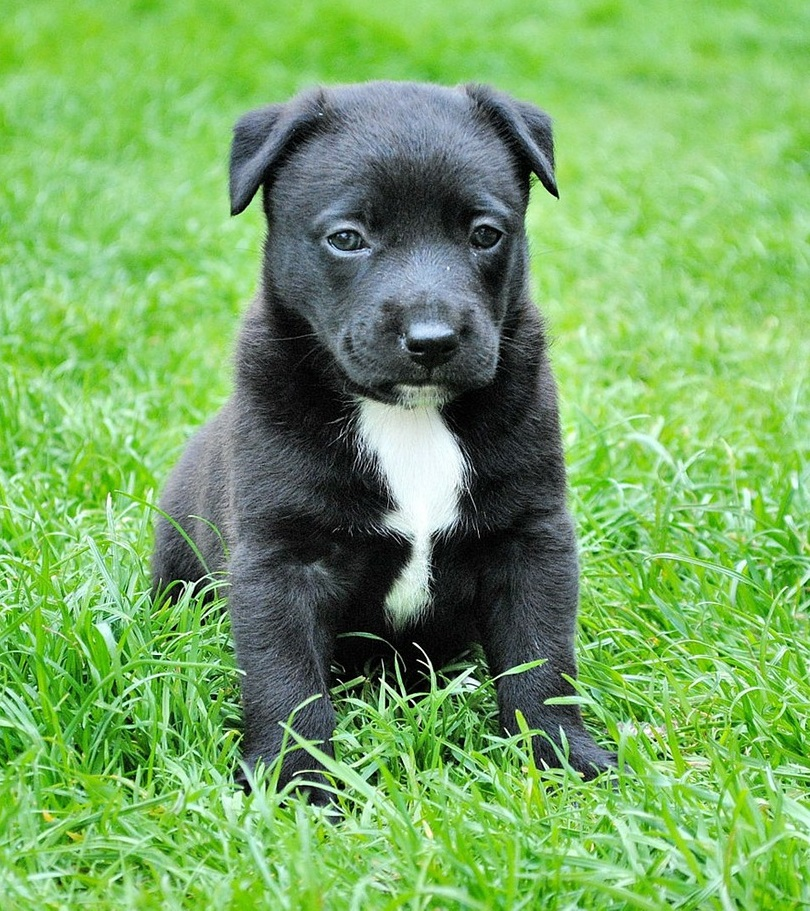
\includegraphics[scale=0.15]{Puppy1}}
In a survey of 400 people, 243 responded that they like dogs.  What percentage of these people like dogs?\\

243 out of 400 $= \dfrac{243}{400} = 0.6075 = 60.75\%$.\\

Roughly 61\% of people responded that they like dogs (this is clearly a very strange sample--there's no way that only 61\% of people like dogs in reality, but hey, this is a math book, not a sociology book).
\end{example}

\begin{try}[http://izzomath.com/103text/finance/example1.3/story.html]
Three of the nine sitting members of the U.S. Supreme Court are female.  What percentage of the court is comprised of women?
\end{try}

\begin{example}[https://www.youtube.com/watch?v=yCQCFHGGHms]{Sales Tax}
Suppose that you load a grocery cart with \$159 worth of groceries, and the local sales tax rate is 7\%. How much tax do you pay, and what is the total cost of the groceries?\\

\marginnote{\bfseries Solution}
The sales tax rate tells you what percentage of the price will be added on top, so we'll calculate 7\% of \$159 and add that to \$159:
\begin{align*}
(\$159)(7\%) = (\$159)(0.07) &= \$11.13\\
&+ \$159 = \$170.13
\end{align*}

\marginnote{\bfseries Alternate Solution}
We could simplify the solution by noticing that we start with 100\% of the cost and add 7\% to it, so we end up with 107\% of the cost: \[(\$159)(107\%) = (\$159)(1.07) = \$170.13\]
\end{example}
\vfill
\pagebreak

Taxes are not much fun to think about, so let's switch briefly to the happier side: discounts.  When you go to a store that advertises a sale of 30\% off, that means that whatever price is on the sticker will get 30\% slashed.  Just like before, we can calculate the new price by finding 30\% of the sticker price and subtracting that.  Alternately, we could notice that if we're removing 30\% of the price, we'll be left with 70\% of the price.  The next example illustrates a similar situation.
%\vfill
%\pagebreak

\begin{example}[https://www.youtube.com/watch?v=eKcXhopfVrU]{Discount}
\marginnote{\includegraphics[scale=0.08]{TV1}}
For months you have been wanting a 47'' LCD flat screen television, but the price has been too high. The store is having a one-day sale on all televisions in the store. For one day only you can take 25\% off any television. The regular price on the television
you want is \$1099.  How much is the sale price?\\

Since the sale takes 25\% off the top of the price, the sale price will be 75\% of the original price:
\[\textrm{Sale price } = (75\%)(\$1099) = (0.75)(\$1099) = \$824.25\]

Notice that we could also find this answer using two steps.  We could find the amount of the discount (by finding 25\% of the price) and then subtract this discount from the original price:
\begin{align*}
\textrm{Discount } &= (25\%)(\$1099) = (0.25)(\$1099) = \$274.75\\
\textrm{Sale Price } &= \textrm{ Original Price } - \textrm{ Discount}\\
&= \$1099.00 - \$274.75 = \$824.25
\end{align*}
Of course, note that we get the same answer either way.  These problems can be done either way, but the first method only required one step rather than two.
\end{example}

\begin{try}[http://izzomath.com/103text/finance/example1.6/story.html]
You have a 20\% off coupon at Bed, Bath, and Beyond, and you're ready to get some new towels.  If you select some that are listed at \$30, and sales tax is 6\%, how much will your final cost be at the register?  Note that the discount is applied \textbf{before} the sales tax.
\end{try}

\vspace*{0.5in}

Another common type of application has to do with \textbf{percentage change}.  For instance, you might hear a presidential candidate promise to cut taxes by 12\%, or you may hear that there are 25\% more hurricanes one year than the year before.  We need to be able to make sense of these claims and ones like them.

\begin{formula}{Relative Change}
The relative change of a quantity is defined as the ratio of the change to the original quantity:
\marginnote{Note carefully that the denominator is the \textbf{original} value, not the final value}
\[\textrm{Relative Change } = \dfrac{\textrm{Absolute Change}}{\textrm{Original Value}} = \dfrac{\textrm{Ending Value} - \textrm{Starting Value}}{\textrm{Starting Value}}\]
This relative change can be written as a fraction or decimal, but it is most commonly used in the form of a percent.
\end{formula}

If the relative change is positive, that means the quantity increased; if the relative change is negative, the quantity decreased.  To find the relative change, we \textit{always} divide by the \textit{original amount}, the amount before the change occurred.
\vfill
\text{}
\pagebreak

\begin{example}[https://www.youtube.com/watch?v=QNzrFqGFBRA]{Car Value}
\marginnote{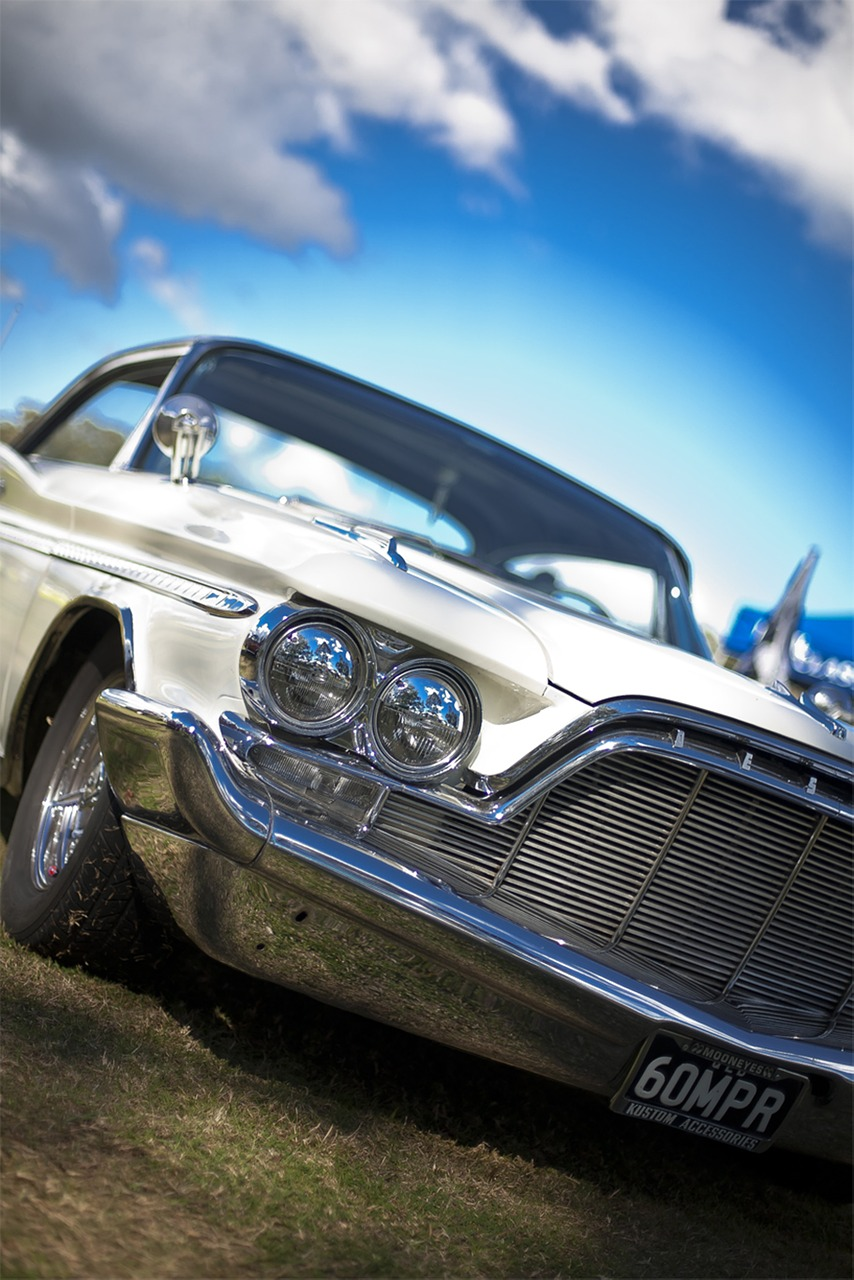
\includegraphics[scale=0.1]{Car1}}
The value of a car dropped from \$7400 to \$6800 over the last year. What percent decrease is this?\\

First, find the absolute change:
\[\$7400 - \$6800 = \$600\]
Then divide this by the \textbf{original amount}:
\[\dfrac{\$600}{\$7400} = 0.081 = 8.1\%\]

Thus, the value of the car dropped by 8.1\%.
\end{example}

\begin{try}[http://izzomath.com/103text/finance/example1.7/story.html]
You go car shopping and find your dream car for \$11,000 sitting on the lot, but unfortunately you only have \$9,000 to pay for it.  You offer the dealership the money you have and they accept your offer.  What percentage did the dealership take off the car?
\end{try}

The base of a percent is very important.  For example, while Nixon was president, it was argued that marijuana is a ``gateway'' drug, using the claim that 80\% of marijuana smokers went on to use harder drugs like cocaine.  The problem is that this isn't true.  The true statistic is that 80\% of harder drug users first smoked marijuana.  The difference is one of base: 80\% of marijuana users versus 80\% of hard drug users.  In reality, out of every 1000 marijuana smokers, about 42 of them go on to use harder drugs, but there are few people who go on to use harder drugs without using marijuana first.

\begin{example}[https://www.youtube.com/watch?v=gB3RqkMzDDE]{Amount Before an Increase}
\marginnote{
\includegraphics[scale=0.08]{Books1}}
If the tuition and fees paid by the average student in the U.S. is \$9,139, and this is 17\% more than the average five years ago, what was the average cost then?\\

The new amount---\$9,139---is 117\% of the original cost:
\[\$9,139 = (117\%)(\textrm{Original Cost})\]
\[\textrm{Original Cost} = \dfrac{\$9,139}{117\%} = \dfrac{\$9,139}{1.17} = \$7,811\]
The original cost, then, was \$7,811 for the average student five years ago.
\end{example}

Relative change or percent differences are also useful when comparing quantities of different sizes, because we can put everything on equal footing to make a meaningful comparison.

\begin{example}[https://www.youtube.com/watch?v=yQmIyPZefK0]{Enrollment Changes}
Generally, more students go to college every semester than the semester before.  In the fall semester of 2008 there were 5,748 students enrolled at Frederick Community College; by the fall of 2009, the number had grown to 6,233.  Compare these two numbers.\\

\marginnote{\bfseries Solution}
We could compare them by simply finding the difference, and saying that there were 485 more students in 2009 than in 2008, but out of context this number is mostly meaningless.  At a small school like FCC, this may represent a dramatic change, but at a larger school like the author's alma mater of North Carolina State, 485 students wouldn't move the needle at all.\\

Instead, we can calculate this as a percentage change:
\[\dfrac{485}{5748} = 0.084 = 8.4\%\]
Enrollment rose by 8.4\%, which is a modest but respectable gain.
\end{example}

\begin{try}[http://izzomath.com/103text/finance/example1.8/story.html]
If you took the SAT twice, scoring 500 on the verbal portion the first time and 620 the second time, by what percentage did your score increase?
\end{try}

This idea of putting different quantities on equal footing in order to compare them is extremely powerful, and crucial in many contexts.  We'll do something similar later when we consider financial applications.  There, we'll be interested in, for instance, comparing two loans with different interest rates and durations and deciding which is more advantageous.  The details will differ, but the concept of finding common ground on which to compare different quantities comes up in many areas.\\

\begin{example}[https://www.youtube.com/watch?v=gSA_go511q4]{Comparisons}
There are 435 Longhorn Steakhouse locations in the U.S. and 136 Ruth's Chris Steakhouse locations.  Compare these two numbers.\\

\marginnote{\bfseries Solution}
Rather than simply saying that there are 299 more Longhorn locations that Ruth's Chris, let's use a meaningful measure like the percentage difference.\\

We could say that Longhorn is \[\frac{299}{136} = 219.9\%\] larger, or that Ruth's Chris is \[\frac{299}{435} = 68.7\%\] smaller.  We could also say that Ruth's Chris is \[\frac{136}{435} = 31.3\%\] of the size of Longhorn.
\end{example}
\text{}\\

The next exercise wraps up the discussion on percentage change by reinforcing the need to be careful with the base of the percent when discussing a change.\\

\begin{example}[https://www.youtube.com/watch?v=SOSt8uYaObc]{A Tricky Percentage Problem}
\marginnote{\includegraphics[scale=0.15]{Taxes1}}
Suppose you originally paid \$1200 in taxes.  A year later taxes decreased by 20\%, but the following year taxes increased by 20\%.  What do you pay in taxes at the end?\\

You may be tempted to jump to the conclusion that you'll pay \$1200 in taxes at the end, since the 20\% decrease was reversed by the 20\% increase.  Be careful, though: the decrease was 20\% of \emph{the original amount} and the increase was 20\% of \emph{the reduced amount}.  Thus, the increase was \emph{smaller} than the increase, so we expect to pay less than \$1200 at the end.\\

Specifically, after one year, the taxes would be $(\$1200)(0.80) = \$960$.  After two years, the taxes would be $(\$960)(1.20) = \$1152$.
\end{example}

\begin{exercises}
\textit{For problems 1--8, convert each number to a percent.}\\
\pfour{$\dfrac{1}{2}$}
\pfour{$0.04$}
\pfour{$\dfrac{3}{5}$}
\pfour{$0.79$}

\pfour{1.35}
\pfour{$\dfrac{10}{4}$}
\pfour{12.5}
\pfour{0.0378}

\textit{For problems 9--16, convert each percent to a decimal.}\\
\pfour{33\%}
\pfour{2.6\%}
\pfour{124\%}
\pfour{1240.5\%}

\pfour{42\%}
\pfour{4.5\%}
\pfour{0.003\%}
\pfour{$\dfrac{1}{4}\%$}

\ptwo{In the fall of 2009 FCC enrolled 6,233 students.  Of those enrolled, 2,810 are in the 18-21 age group.  What percent of FCC students does this represent?}
\ptwo{Patrick left an \$8 tip on a \$50 restaurant bill.  What percent tip is that?}

\ptwo{Ireland has a 23\% VAT (value-added tax, similar to a sales tax).  How much will the VAT be on a purchase of a \euro 250 item?}
\ptwo{Employees in 2012 paid 4.2\% of their gross wages towards social security (FICA tax).  How much would someone earning \$45,000 a year pay toward social security?}

\ptwo{A project on Kickstarter was aiming to raise \$15,000 for a precision coffee press.  They ended up with 714 supporters, raising 557\% of their goal.  How much did they raise?}
\ptwo{Another Kickstarter project for an iPad stylus raised 1,253\% of their goal, finishing with a total of \$313,250 from 7,511 supporters.  What was their original goal?}

\ptwo{One year ago the median price for a home was \$275,000.  Now the current median price for a home is \$235,000.  What was the percent decrease in the median price of a home over the last year?}
\ptwo{There were 943 tornadoes reported in the U.S. in 2013, and 897 tornadoes were reported in 2014.  What percent decrease was there from 2013 to 2014?}

\ptwo{The population of a town increased from 3,250 in 2008 to 4,300 in 2010.  Find the absolute increase and the percent increase.}
\ptwo{The number of CDs sold in 2010 was 114 million, down from 147 million the previous year.  Find the absolute decrease and the percent decrease.}

\ptwo{A company wants to decrease their energy use by 15\%.
\begin{enumerate}[(a)]
\item If their electric bill is currently \$2,200 a month, what will their bill be if they're successful?
\item If their next bill is \$1,700 a month, were they successful?  What percent decrease was there from the current bill?
\end{enumerate}
}
\ptwo{A store is hoping an advertising campaign will increase their number of customers by 30\%.  They currently have about 80 customers per day.
\begin{enumerate}[(a)]
\item How many customers will they have if their campaign is successful?
\item If they increase to 120 customers a day, were they successful?  What percent increase is this from the current level?
\end{enumerate}
}

\ptwo{An article reports that ``attendance dropped 6\% this year, to 300.''  What was the attendance before the drop?}
\ptwo{An article reports that ``sales have grown by 30\% this year, to \$200 million.''  What were sales before the growth?}

\ptwo{The U.S. federal debt at the end of 2001 was \$5.77 trillion, and grew to \$6.20 trillion by the end of 2002. At the end of 2005 it was \$7.91 trillion, and grew to \$8.45 trillion by the end of 2006. Calculate the absolute and relative increase for 2001-2002 and 2005-2006. Which year saw a larger increase in federal debt?}
\ptwo{A TV originally priced at \$799 is on sale for 30\% off. There is then a 9.2\% sales tax. Find the price after including the discount and sales tax.}

\ptwo{The Walden University had 47,456 students in 2010, while Kaplan University had 77,966 students.  Complete the following statements.
\begin{enumerate}[(a)]
\item Kaplan's enrollment was \line(1,0){20} \% larger than Walden's.
\item Walden's enrollment was \line(1,0){20} \% smaller than Kaplan's.
\item Walden's enrollment was \line(1,0){20} \% of Kaplan's.
\end{enumerate}}
\ptwo{In the 2012 Olympics, Usain Bolt ran the 100 m dash in 9.63 seconds.  Jim Hines won the 1968 gold with a time of 9.95 seconds.
\begin{enumerate}[(a)]
\item Bolt's time was \line(1,0){20} \% faster than Hines'.
\item Hines' time was \line(1,0){20} \% slower than Bolt's.
\item Hines' time was \line(1,0){20} \% of Bolt's.
\end{enumerate}}

\ptwo{A store has clearance items that have been marked down by 60\%.  They are having a sale, advertising an additional 30\% off clearance items.  What percent of the original price do you end up paying?}
\ptwo{A publisher marks up a textbook by 65\%, and a bookstore further marks up the textbook by 35\%.  What percentage of the original cost do you pay?}
\end{exercises}


\section{Income Tax}
\setcounter{ExampleCounter}{1}
While taxes are not typically greeted with great enthusiasm, they are a necessary part of life.  Governments---whether city, county, state, or federal---depend on tax revenue to fund their projects.  For instance, gasoline taxes fund road maintenance, property taxes fund schools, and federal income taxes fund thousands of initiatives from the Food and Drug Administration to the military.  Our focus in this section will be on the federal income tax, but first we'll look at a few different kinds of tax.

Typically, taxes are calculated as a percentage of a sale (we've already dealt with sales tax in the previous section), the percentage of one's assets (as with an estate tax or a property tax), or the percentage of one's income (as with the federal or state income tax).

\begin{proc}{Effective Tax Rate}
When taxes are given as an amount rather than a percentage, we can calculate the \textbf{effective tax rate} in order to compare it to other taxes on the same basis.
\end{proc}

\begin{example}[https://www.youtube.com/watch?v=QjjpqBp5d6w]{Property Taxes}
Joan paid \$3,200 in property taxes on her house, which was valued at \$215,000 last year.  What is the effective property tax rate?\\

\marginnote{\bfseries Solution}
The equivalent percentage is \[\dfrac{3,200}{215,000} = 0.01488 = 1.49\%\]
\end{example}

\begin{example}[https://www.youtube.com/watch?v=tyNOEV7Q7xg]{Gasoline Tax}
\marginnote{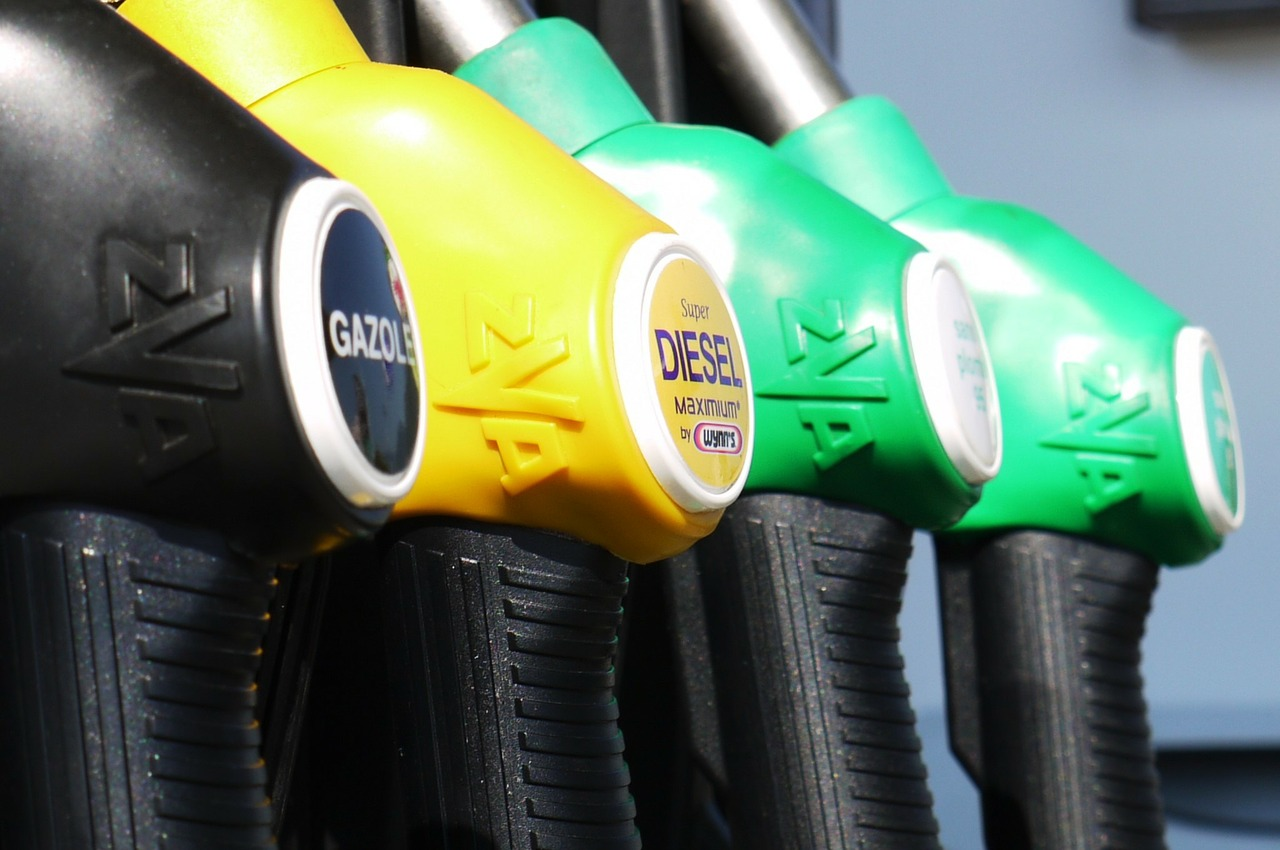
\includegraphics[scale=0.07]{GasPump1}}
If the state gas tax is 30.3 cents per gallon, and the pre-tax cost of gasoline is \$2.42 per gallon, what is the gas tax rate?\\

The equivalent percentage is \[\dfrac{\$0.303}{\$2.42} = 12.52\%\]
\end{example}

\begin{try}[http://izzomath.com/103text/finance/example2.1/story.html]
If you pay \$35.75 in sales tax on a \$550 purchase, what is the effective sales tax?
\end{try}

Some taxes---like these examples of sales tax, property tax, and gas tax---are a \textbf{flat tax}, since the tax percentage is constant no matter what the amount of the sale or the value of the property.  Many taxes---most notably, federal and state income taxes---are not flat, but instead are \textbf{progressive taxes}, meaning that the tax percentage increases as the taxpayer's income increases, so taxpayers who earn more pay a higher tax rate than those who earn less.  The reverse situation is a \textbf{regressive tax}, where the tax rate decreases as the taxed amount increases.

\begin{formula}{Tax Categories}
\begin{itemize}
\item \marginnote{ex: sales tax}A \textbf{flat tax} charges a consistent percentage, no matter what the taxed amount is.
\item \marginnote{ex: income tax}A \textbf{progressive tax} charges a higher percentage for higher taxed amounts.
\item A \textbf{regressive tax} charges a lower percentage for higher taxed amounts.
\end{itemize}
\end{formula}
\vfill
\pagebreak

Now let's talk about the U.S. federal income tax, the most prominent example of a progressive tax that you're likely to encounter.  Each taxpayer's earnings are split into \textbf{tax brackets}, and each tax bracket is taxed at a certain rate.  So for instance, in 2014, a single taxpayer's first \$9075 were taxed at 10\%, and every dollar from number 9076 up to dollar number 36,900 was taxed at 15\%.  To figure out how much someone owes, we need to split their taxable income into these brackets (assume this taxpayer earns \$89,350 per year):

\begin{center}
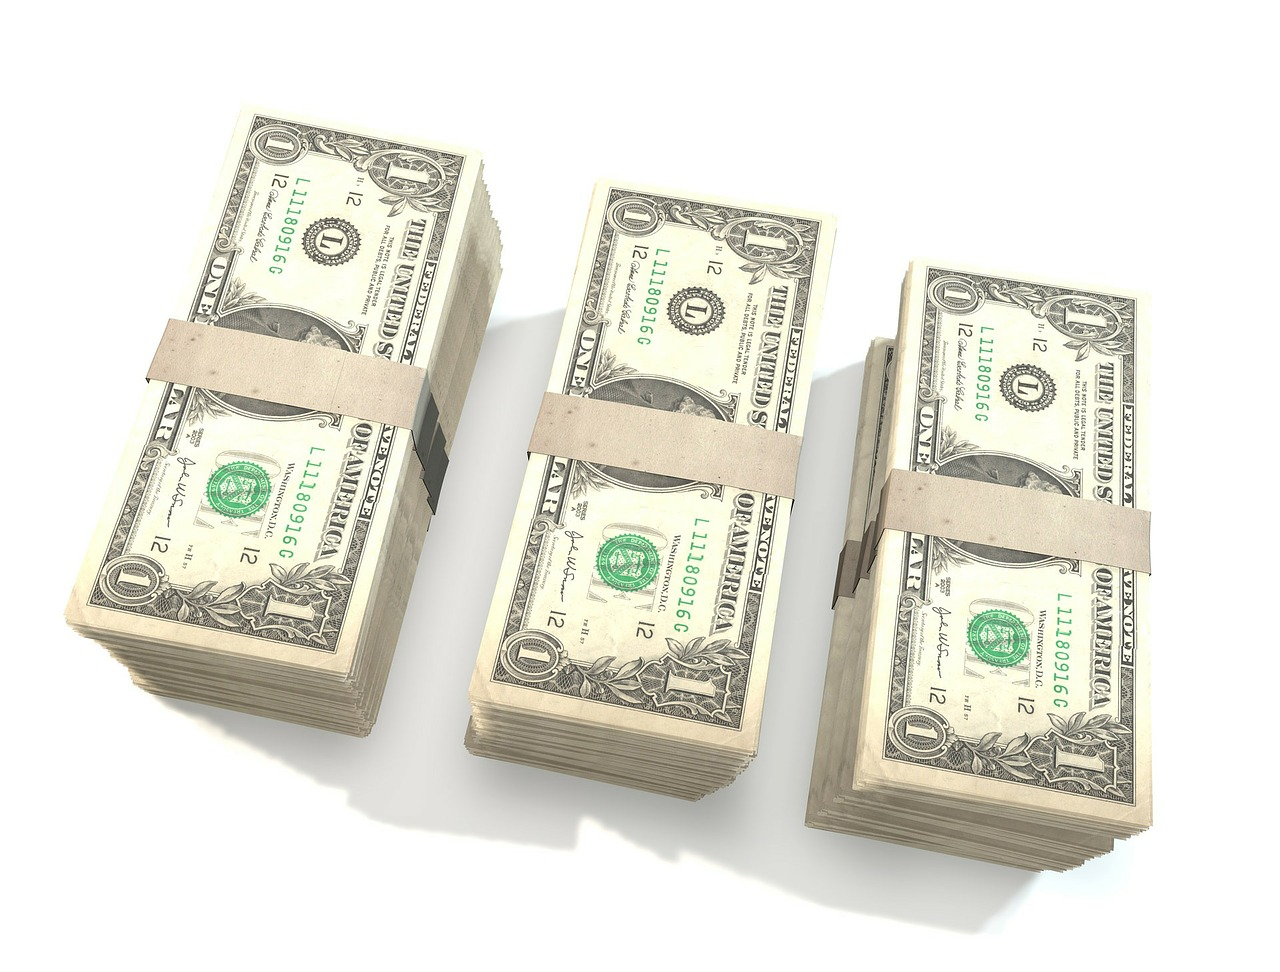
\includegraphics[scale=0.07]{Dollars1}

\begin{tcolorbox}[colframe=green!5,colback=green!5,sharp corners=all]
\begin{center}
\$89,350

$\overbrace{
\begin{tabular}{r | c c c}
& & & \\
\marginnote{Split money into brackets}Dollars & 1 -- 9075 & 9076 -- 36,900 & 36,901 -- 89,350\\
& & & \\
Tax Rate & 10\% & 15\% & 25\%\\
& & & \\
\marginnote{Multiply the amount in each }Calculation & \$9075(0.1) & (\$36,900 -- \$9075)(0.15) & (\$89,350 -- \$36,900)(0.25)\\
& & & \\
\marginnote{bracket by the tax rate}& = \$907.50 & = \$4173.75 & = \$13,112.50
\end{tabular}
}$
\vspace{0.25in}

This taxpayer pays $\$907.50 + \$4,173.75 + \$13,112.50 = \$18,193.75$ in taxes.

\end{center}
\end{tcolorbox}
\end{center}

No matter whether you make \$30,000 a year or \$300,000 per year, your first \$9075 are taxed at the same rate; it's the later dollars that get taxed at a higher rate, making this a progressive tax.

The tax rates for each bracket may change from year to year, but the process remains the same:
\begin{enumerate}
\item Divide the taxable income into these brackets, putting each dollar into the appropriate bracket until you get to the end of the income (so if the taxpayer's income in the example above was \$32,000, we would have stopped in the second bracket and not spilled over into the third).
\item Multiply the amount in each bracket by the tax rate for that bracket.
\item Add up the tax amounts from each bracket to find the total income tax owed.
\end{enumerate}

The following table is the marginal tax table for 2014, showing the tax brackets and associated tax rate for each.
\vspace{0.25in}

\label{Tax Table}
\checkoddpage
\ifoddpage{
\begin{adjustwidth}{-0.25in}{-1.5in}
\begin{center}
\begin{tabular}{| p{0.85in} | p{1.35in} | p{1.35in} | p{1.5in} | p{1.35in} |}
\hline
\cellcolor{brown!25}Tax Rate & \cellcolor{brown!25}Single & \cellcolor{brown!25}Married Filing Separately & \cellcolor{brown!25}Married Filing Jointly & \cellcolor{brown!25}Head of Household\\
\hline
\cellcolor{brown!25}10\% & up to \$9,075 & up to \$9,075 & up to \$18,150 & up to \$12,950\\
\hline
\cellcolor{brown!25}15\% & \$9,075 to \$36,900 & \$9,075 to \$36,900 & \$18,150 to \$73,800 & \$12,950 to \$49,400\\
\hline
\cellcolor{brown!25}25\% & \$36,900 to \$89,350 & \$36,900 to \$74,425 & \$73,800 to \$148,850 & \$49,400 to \$127,550\\
\hline
\cellcolor{brown!25}28\% & \$89,350 to \$186,350 & \$74,425 to \$113,425 & \$148,850 to \$226,850 & \$127,550 to \$206,600\\
\hline
\cellcolor{brown!25}33\% & \$186,350 to \$405,100 & \$113,425 to \$202,550 & \$226,850 to \$405,100 & \$206,600 to \$405,100\\
\hline
\cellcolor{brown!25}35\% & \$405,100 to \$406,750 & \$202,550 to \$228,800 & \$405,100 to \$457,600 & \$405,100 to \$432,200\\
\hline
\cellcolor{brown!25}39.6\% & more than \$406,750 & more than \$228,800 & more than \$457,600 & more than \$432,200\\
\hline
\cellcolor{brown!25}Standard Deduction & \$6,200 & \$6,200 & \$12,400 & \$9,100\\
\hline
\cellcolor{brown!25}Exemptions (per person) & \$3950 & \$3950 & \$3950 & \$3950\\
\hline
\end{tabular}
\end{center}
\end{adjustwidth}
\vspace{0.25in}}
\else{\begin{adjustwidth}{-1.75in}{-0.25in}
\begin{center}
\begin{tabular}{| p{0.85in} | p{1.35in} | p{1.35in} | p{1.5in} | p{1.35in} |}
\hline
\cellcolor{brown!25}Tax Rate & \cellcolor{brown!25}Single & \cellcolor{brown!25}Married Filing Separately & \cellcolor{brown!25}Married Filing Jointly & \cellcolor{brown!25}Head of Household\\
\hline
\cellcolor{brown!25}10\% & up to \$9,075 & up to \$9,075 & up to \$18,150 & up to \$12,950\\
\hline
\cellcolor{brown!25}15\% & \$9,075 to \$36,900 & \$9,075 to \$36,900 & \$18,150 to \$73,800 & \$12,950 to \$49,400\\
\hline
\cellcolor{brown!25}25\% & \$36,900 to \$89,350 & \$36,900 to \$74,425 & \$73,800 to \$148,850 & \$49,400 to \$127,550\\
\hline
\cellcolor{brown!25}28\% & \$89,350 to \$186,350 & \$74,425 to \$113,425 & \$148,850 to \$226,850 & \$127,550 to \$206,600\\
\hline
\cellcolor{brown!25}33\% & \$186,350 to \$405,100 & \$113,425 to \$202,550 & \$226,850 to \$405,100 & \$206,600 to \$405,100\\
\hline
\cellcolor{brown!25}35\% & \$405,100 to \$406,750 & \$202,550 to \$228,800 & \$405,100 to \$457,600 & \$405,100 to \$432,200\\
\hline
\cellcolor{brown!25}39.6\% & more than \$406,750 & more than \$228,800 & more than \$457,600 & more than \$432,200\\
\hline
\cellcolor{brown!25}Standard Deduction & \$6,200 & \$6,200 & \$12,400 & \$9,100\\
\hline
\cellcolor{brown!25}Exemptions (per person) & \$3950 & \$3950 & \$3950 & \$3950\\
\hline
\end{tabular}
\end{center}
\end{adjustwidth}
\vspace{0.25in}}
\fi

Note that there are two rows at the end of the table that contain terms we haven't defined yet; fear not, we'll get to these momentarily.  Also, the term `Head of Household' simply means a single individual who is paying more than half the cost of supporting a child or parent.
\vfill
\pagebreak

\begin{example}[https://www.youtube.com/watch?v=p7ofzArnTxo]{Income Tax}
Using the tax table above, how much would a married taxpayer who files separately from their spouse owe on a taxable income of \$98,400?\\

\marginnote{\bfseries Solution}
First, note that we'll be using the second column, since this taxpayer is married, filing separately.  Next, divide the \$98,400 into the appropriate brackets:

\begin{center}
\$98,400

$\overbrace{
\begin{tabular}{r | c c c c}
& & & \\
Dollars & 1 -- 9075 & 9076 -- 36,900 & 36,901 -- 74,425 & 74,426 -- 98,400\\
& & & \\
Tax Rate & 10\% & 15\% & 25\% & 28\%\\
\end{tabular}
}$
\end{center}

Then simply multiply the amount in each bracket by that tax rate and add up these totals:
\begin{align*}
\textrm{Tax Owed } &= (9,075)(0.1) + (36,900-9,075)(0.15)\\ &\hspace{0.5in} + (74,425-36,900)(0.25) + (98,400-74,425)(0.28)\\ &= \$21,175.50
\end{align*}
\end{example}

\begin{try}[http://izzomath.com/103text/finance/example2.3/story.html]
Using the 2014 marginal tax table, how much would a head of household owe on a taxable income of \$77,000?
\end{try}

We've used the term ``taxable income'' several times without defining it, since it is fairly self-explanatory.  However, a big part of the complexity of income taxes has to do with the terminology, so let's define a few terms here:

\begin{formula}{Income Tax Terms}
\begin{itemize}
\item \textbf{Gross Income:} Total yearly income.  This is the number the taxpayer starts with, the total amount earned, including wages, tips, capital gains, and unemployment.\marginnote{\centering\bfseries Gross income}
\item The following three are deducted from the gross income:
\begin{itemize}
\item \marginnote{\centering $-$}\textbf{Adjustments:} This category includes things like student loan interest, moving expenses, health insurance expenses, and alimony.\marginnote{\centering Adjustments}
\item \marginnote{\centering $-$}\textbf{Exemptions:} A fixed amount determined for each year and listed on the marginal tax table.  \marginnote{\centering Exemptions}Each taxpayer gets one exemption for themselves, and one exemption for each dependent.\marginnote{\centering $-$}
\item \marginnote{\centering Deductions}\textbf{Deductions:} The taxpayer can choose between two options:
\begin{enumerate}
\item Take the standard deduction.  This is another fixed amount listed on the marginal tax table.\marginnote{\centering $=$}
\item Calculate an itemized deduction.  This includes things like interest on a home mortgage, charitable donations, and property taxes.
\end{enumerate}
\marginnote{\centering\bfseries Taxable income}Each taxpayer picks whichever one is higher, thus taking more off of their gross income.\marginnote{\centering $\downarrow$}
\end{itemize}
\item \marginnote{\centering Initial Tax Owed}\textbf{Taxable Income:} This is the income that is used, like in the previous examples, with the marginal tax table to calculate the tax that is owed.\marginnote{\centering $-$}
\item \marginnote{\centering\bfseries Tax credits}\textbf{Tax Credits:} These are deducted, not from the income, but from the tax owed.  \marginnote{\centering $=$}They include things, like child care, education credits, or energy savings.  Typically tax credits are used to reward behavior that the administration at the time wants to incentivize.\marginnote{\centering\bfseries Final Tax Owed}
\end{itemize}
\end{formula}
\vfill
\pagebreak

Essentially, it all begins with the gross income, from which the adjustments, exemptions, and deductions are whittled away, leaving a smaller amount as the taxable income (this works in the taxpayer's favor, obviously).  After taxes are calculated on this taxable income using the marginal tax table like the one on page \pageref{Tax Table}, tax credits are deducted from that answer, leaving the final taxes owed.

Thus, in the actual calculation, the adjustments, exemptions, and deductions are treated the same way; the only difference is in what each term means and what kinds of spending fall under each category.  In the examples that we'll see, the adjustments and deductions are listed clearly, but exemptions are not listed; you'll need to remember to account for exemptions, depending on how many dependents a particular taxpayer has.

\begin{example}[https://www.youtube.com/watch?v=_kXpgV9IAng]{Tax Calculation}
Use the 2014 marginal tax table on page \pageref{Tax Table} to calculate the tax owed by a single woman with no dependents whose details are given below.
\begin{center}
\begin{tabular}{r l}
Gross income: & \$65,000\\
Adjustments: & \$2000\\
Deductions: & \$3000: charitable donations\\
& \$1500: theft loss\\
& \$300: cost of tax preparation\\
Tax credit: & \$500: energy-efficient appliances
\end{tabular}
\end{center}

\marginnote{\bfseries Solution}Start by subtracting the adjustments, exemption, and deductions from the gross income:
\begin{alignat*}{7}\marginnote{Find the taxable income}
&\textrm{Gross income } &&- \textrm{ Adjustments } &&- \textrm{ Exemptions } &&- \textrm{ Deductions }\\
&= \$65,000 &&- \$2000 &&- \$3950 &&- \$6200\\
&= \$52,850
\end{alignat*}

Notice that rather than using the itemized deductions, she chose the standard deduction, since it was larger than the sum of the itemized deductions.

Next, take the taxable income and split it into the marginal categories, then calculate the tax owed from each bracket:
\begin{center}
\$52,850\marginnote{Divide the taxable income into brackets}

$\overbrace{
\begin{tabular}{r | c c c}
& & & \\
Dollars & 1 -- 9075 & 9076 -- 36,900 & 36,901 -- 52,850\\
%& & & \\
Tax Rate & 10\% & 15\% & 25\%\\
\end{tabular}
}$
\end{center}
\begin{align*}\marginnote{Multiply the amount in each bracket by that tax rate}
\textrm{Tax Owed } &= (9,075)(0.1) + (36,900-9,075)(0.15)\\ &\hspace{0.5in} + (52,850-36,900)(0.25)\\ &= \$9068.75
\end{align*}

Finally, subtract the tax credit from this initial tax calculation to find the final amount that she owes:

\marginnote{Subtract the tax credit}\[\textrm{Final Tax Owed } = \$9068.75 - \$500 = \$8568.75\]
\end{example}

\begin{try}[http://izzomath.com/103text/finance/example2.4/story.html]
Use the 2014 marginal tax table to calculate the tax owed by a married couple with no dependents filing jointly whose details are given below.
\begin{center}
\begin{tabular}{r l}
Gross income: & \$74,000\\
Adjustments: & \$1500\\
Deductions: & \$5500: charitable donations\\
& \$150: cost of tax preparation\\
Tax credit: & \$700: earned income tax credit
\end{tabular}
\end{center}
\end{try}
\vfill
\pagebreak

\checkoddpage
\ifoddpage{
\begin{adjustwidth}{0in}{-1.25in}
\begin{proc}{Tax Withholding}
During World War II, when the U.S. government was in dire need of tax revenue in order to avoid the rampant inflation that occurred during World War I, the IRS began to investigate tax withholding.  Rather than collecting taxes at the end of the year, they began to withhold taxes from workers' paychecks throughout the year, and then make up the difference at the end, either by a refund or an extra tax payment.  Milton Friedman, who won the 1976 Nobel Prize in economics, helped to formulate this plan.\\

New employees fill out a W-4 form, which is intended to calculate as accurately as possible how much they'll owe in taxes, so that the correct amount can be collected.  Many people like the idea of overestimating, because if more is withheld throughout the year, they receive a huge refund check.  However, this is not actually a good policy, since in effect they are giving the government an interest-free loan for the entire year with no strings attached.
\end{proc}
\end{adjustwidth}
} \else{
\begin{adjustwidth}{-1.25in}{0in}
\begin{proc}{Tax Withholding}
During World War II, when the U.S. government was in dire need of tax revenue in order to avoid the rampant inflation that occurred during World War I, the IRS began to investigate tax withholding.  Rather than collecting taxes at the end of the year, they began to withhold taxes from workers' paychecks throughout the year, and then make up the difference at the end, either by a refund or an extra tax payment.  It was Milton Friedman, who won the 1976 Nobel Prize in economics, who helped to formulate this plan.\\

New employees fill out a W-4 form, which is intended to calculate as accurately as possible how much they'll owe in taxes, so that the correct amount can be collected.  Many people like the idea of overestimating, because if more is withheld throughout the year, they receive a huge refund check.  However, this is not actually a good policy, since in effect they are giving the government an interest-free loan for the entire year with no strings attached.
\end{proc}
\end{adjustwidth}
} \fi

\begin{example}[https://www.youtube.com/watch?v=VeMJEVdRfMk]{Tax Calculation}
Use the 2014 marginal tax table on page \pageref{Tax Table} to calculate the tax owed by a head of household with three dependents whose details are given below.
\begin{center}
\begin{tabular}{r l}
Gross income: & \$58,000\\
Adjustments: & \$2300\\
Deductions: & none\\
Tax credit: & none
\end{tabular}
\end{center}

\marginnote{\bfseries Solution}Start by subtracting the adjustments, exemption, and deductions from the gross income:
\begin{alignat*}{7}\marginnote{Find the taxable income}
&\textrm{Gross income } &&- \textrm{ Adjustments } &&- \textrm{ Exemptions } &&- \textrm{ Deductions }\\
&= \$58,000 &&- \$2300 &&- (4)\$3950 &&- \$6200\\
&= \$33,700
\end{alignat*}

Again, we use the standard deduction.  Notice that this time, there are four exemptions, one for the taxpayer and one for each of the dependents.

Next, take the taxable income and split it into the marginal categories, then calculate the tax owed from each bracket:
\begin{center}
\$33,700\marginnote{Divide the taxable income into brackets}

$\overbrace{
\begin{tabular}{r | c c}
& & \\
Dollars & 1 -- 9075 & 9076 -- 33,700\\
%& &  \\
Tax Rate & 10\% & 15\%\\
\end{tabular}
}$
\end{center}
\begin{align*}\marginnote{Multiply the amount in each bracket by that tax rate}
\textrm{Tax Owed } &= (9,075)(0.1) + (33,700-9,075)(0.15)\\ &= \$4601.25
\end{align*}

There are no tax credits, so this is the final tax owed.
\end{example}

\begin{exercises}

\pthree{A \line(1,0){75} \ is a tax at a consistent rate.}
\pthree{A \line(1,0){75} \ is a tax for which the rate increases for higher taxed amounts}
\pthree{A \line(1,0){75} \ is a tax for which the rate decreases for higher taxed amounts}

\pthree{If the property taxes are \$1800 on a home valued at \$140,000, what is the effective tax rate?}
\pthree{In state A, the gas tax is 28 cents per gallon, where the average pre-tax cost of gas is \$2.58 per gallon.  In state B, the gas tax is 25 cents per gallon, where the average pre-tax cost of gas is \$2.50.  Which state has a lower gas tax rate?}
\pthree{If the sales tax is \$16.05 on a purchase of \$214, what is the sales tax rate?}

\noindent \textit{For problems 7--14, use the marginal tax table on page \pageref{Tax Table} to calculate the tax owed by each taxpayer.}

\ptwo{\\
\begin{tabular}{r l}
Taxpayer: & Single\\
Gross income: & \$75,000\\
Dependents: & 2\\
Adjustments: & \$2000\\
Deductions: & \$28,000: mortgage interest\\
& \$4500: property taxes\\
& \$2000: charitable donations\\
& \$300: cost of tax preparation\\
Tax credit: & \$800
\end{tabular}}
\ptwo{\\
\begin{tabular}{r l}
Taxpayer: & Single\\
Gross income: & \$60,000\\
Dependents: & none\\
Adjustments: & \$1400\\
Deductions: & \$15,000: mortgage interest\\
& \$2000: property taxes\\
& \$3000: charitable donations\\
Tax credit: & \$1300
\end{tabular}}

\ptwo{\\
\begin{tabular}{r l}
Taxpayer: & Married, filing separately\\
Gross income: & \$85,500\\
Dependents: & 1\\
Adjustments: & \$4000\\
Deductions: & \$5000: charitable donations\\
& \$3750: state taxes\\
Tax credit: & \$750
\end{tabular}}
\ptwo{\\
\begin{tabular}{r l}
Taxpayer: & Married, filing separately\\
Gross income: & \$52,000\\
Dependents: & none\\
Adjustments: & \$3300\\
Deductions: & \$4500: charitable donations\\
& \$1500: theft loss\\
& \$1800: state taxes\\
Tax credit: & \$1400
\end{tabular}}

\ptwo{\\
\begin{tabular}{r l}
Taxpayer: & Married, filing jointly\\
Gross income: & \$104,000\\
Dependents: & 4\\
Adjustments: & \$6000\\
Deductions: & \$18,000: mortgage interest\\
& \$5300: property taxes\\
& \$4800: state taxes\\
Tax credit: & none
\end{tabular}}
\ptwo{\\
\begin{tabular}{r l}
Taxpayer: & Married, filing jointly\\
Gross income: & \$93,000\\
Dependents: & none\\
Adjustments: & \$5500\\
Deductions: & \$24,000: mortgage interest\\
& \$3700: property taxes\\
& \$3650: state taxes\\
Tax credit: & none
\end{tabular}}

\ptwo{\\
\begin{tabular}{r l}
Taxpayer: & Head of Household\\
Gross income: & \$25,000\\
Dependents: & 3\\
Adjustments: & none\\
Deductions: & none\\
Tax credit: & \$200
\end{tabular}}
\ptwo{\\
\begin{tabular}{r l}
Taxpayer: & Head of Household\\
Gross income: & \$61,000\\
Dependents: & 4\\
Adjustments: & \$1800\\
Deductions: & \$15,000: mortgage interest\\
& \$2200: property taxes\\
& \$2150: state taxes\\
Tax credit: & none
\end{tabular}}
\vfill
\pagebreak

\pone{\textbf{Project: Flat Tax, Modified Flat Tax, and Progressive Tax}

Many people have proposed various revisions to the income tax collection in the U.S.  Some, for example (including Milton Friedman), have claimed that a flat tax would be fairer.  Others call for revisions to how different types of income are taxed.  This project is for you to investigate this idea.\\

Imagine the country is made up of 100 households.  The federal government needs to collect \$800,000 in income taxes to be able to function (this is roughly proportional to the actual U.S. population and tax needs, but using smaller, more manageable numbers).  The population consists of 6 groups:
\begin{center}
\begin{tabular}{r l}
Group A: & 20 households that earn \$12,000 each\\
Group B: & 20 households that earn \$29,000 each\\
Group C: & 20 households that earn \$50,000 each\\
Group D: & 20 households that earn \$79,000 each\\
Group E: & 15 households that earn \$129,000 each\\
Group F: & 5 households that earn \$295,000 each
\end{tabular}
\end{center}
We are going to determine new income tax rates.

\paragraph{Proposal A} The first proposal we'll consider is a flat tax --- one where every income group is taxed at the same percentage rate.
\begin{enumerate}[1)]
\item Determine the total income for the population.
\vspace{1in}

\item Determine what flat tax rate would be necessary to collect enough money.
\vspace{1in}
\end{enumerate}

\paragraph{Proposal B} The second proposal we'll consider is a modified flat-tax plan, where everyone only pays taxes on any income over \$20,000.  So everyone is Group A will pay no taxes, for instance, and everyone in Group B will pay taxes only on \$9,000.
\begin{enumerate}[1)]
\setcounter{enumi}{2}
\item Determine the total \textit{taxable} income for the population.
\vspace{1in}

\item Determine what flat tax rate would be necessary to collect enough money in this modified system.
\end{enumerate}
}
\vfill
\pagebreak

\begin{minipage}[t]{\textwidth}
\begin{enumerate}[1)]
\setcounter{enumi}{4}
\item Complete the table below for both plans.
\end{enumerate}

\begin{center}
\begin{tabular}{|c | p{0.75in} | p{1.1in} | p{0.85in} | p{1.1in} | p{0.85in} |}
\hline
\multicolumn{2}{|c|}{} & \multicolumn{2}{c|}{Flat Tax Plan} & \multicolumn{2}{c|}{Modified Flat Tax Plan}\\
\hline
Group & Income per Household & Income Tax per Household & Income After Taxes & Income Tax per Household & Income After Taxes\\
\hline
& & & & & \\
A & \$12,000 & & & & \\
& & & & & \\
\hline
& & & & & \\
B & \$29,000 & & & & \\
& & & & & \\
\hline
& & & & & \\
C & \$50,000 & & & & \\
& & & & & \\
\hline
& & & & & \\
D & \$79,000 & & & & \\
& & & & & \\
\hline
& & & & & \\
E & \$129,000 & & & & \\
& & & & & \\
\hline
& & & & & \\
F & \$295,000 & & & & \\
& & & & & \\
\hline
\end{tabular}
\end{center}

\paragraph{Proposal C} The third proposal we'll consider is a progressive tax, where lower income groups are taxed at a lower percentage rate and higher income groups are taxed at a higher percentage rate.  For simplicity, we're going to assume that a household is taxed at the same rate on \textit{all} their income.
\begin{enumerate}[1)]
\setcounter{enumi}{5}
\item Set progressive tax rates for each income group to bring in enough money.  There is no single right answer here --- just make sure you bring in enough money (the total tax must add up to at least \$800,000)!\\
\begin{tabular}{|c | p{0.75in} | p{0.9in} | p{1.1in} | p{1.3in} | p{1.3in} |}
\hline
Group & Income per Household & Tax Rate (\%) & Income Tax per Household & Total Tax Collected for All Households & Income After Taxes per Household\\
\hline
& & & & & \\
A & \$12,000 & & & & \\
& & & & & \\
\hline
& & & & & \\
B & \$29,000 & & & & \\
& & & & & \\
\hline
& & & & & \\
C & \$50,000 & & & & \\
& & & & & \\
\hline
& & & & & \\
D & \$79,000 & & & & \\
& & & & & \\
\hline
& & & & & \\
E & \$129,000 & & & & \\
& & & & & \\
\hline
& & & & & \\
F & \$295,000 & & & & \\
& & & & & \\
\hline
\end{tabular}
\end{enumerate}
\end{minipage}

\begin{minipage}[t]{\textwidth}
\begin{enumerate}[1)]
\setcounter{enumi}{6}
\item Discretionary income is the income people have left over after paying for necessities like rent, food, transportation, etc.  The cost of basic expenses does increase with income, since housing and car costs are higher.  However, these increases are usually not proportional to the increase in income.  For each income group, estimate their essential expenses and calculate their discretionary income.  Then compute the effective tax rate for each plan relative to discretionary income rather than income.
\begin{center}
\begin{tabular}{|c | p{0.75in} | p{1.3in} | p{0.75in} | p{1in} | p{1in} |}
\hline
Group & Income per Household & Discretionary Income (estimated) & Effective Rate, Flat & Effective Rate, Modified & Effective Rate, Progressive\\
\hline
& & & & & \\
A & \$12,000 & & & & \\
& & & & & \\
\hline
& & & & & \\
B & \$29,000 & & & & \\
& & & & & \\
\hline
& & & & & \\
C & \$50,000 & & & & \\
& & & & & \\
\hline
& & & & & \\
D & \$79,000 & & & & \\
& & & & & \\
\hline
& & & & & \\
E & \$129,000 & & & & \\
& & & & & \\
\hline
& & & & & \\
F & \$295,000 & & & & \\
& & & & & \\
\hline
\end{tabular}
\end{center}

\item Which plan seems the most fair to you?  Which plan seems the least fair to you?  Why?
\end{enumerate}
\end{minipage}
\end{exercises}

\section{Simple and Compound Interest}
\setcounter{ExampleCounter}{1}
\marginnote{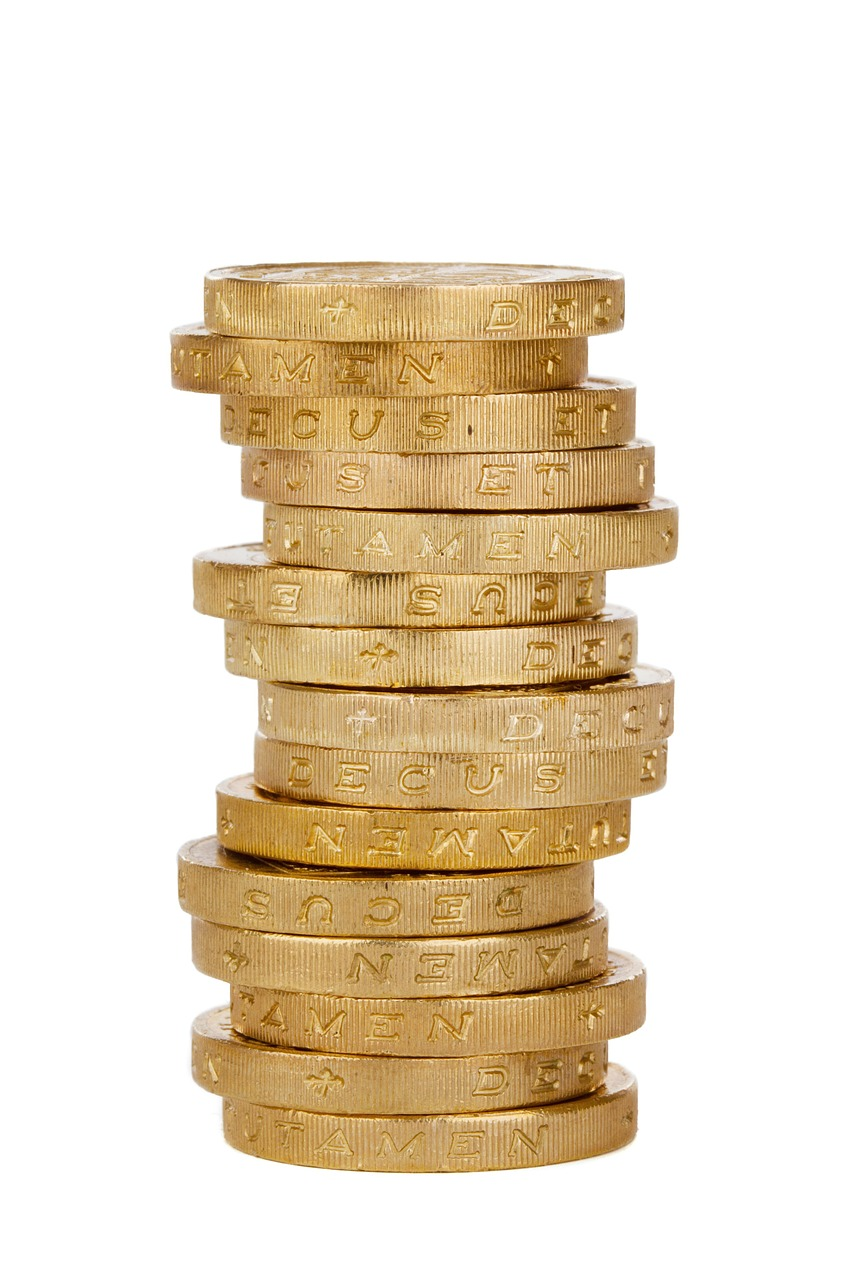
\includegraphics[scale=0.05]{Coins1}}
The basic goal of business (as simplistic as it sounds) is to take a small pile of money and turn it into a big pile of money.  This is capitalism explained in a single sentence.  Because of that, there is value to holding money, because you can use it to make more money.\\  

For instance, say you want to start a landscaping business.  It's unlikely that you would have enough money lying around to do so, so you would take out a small business loan and use that money to buy a truck, a trailer, lawn mowers, blowers, rakes, etc.  Maybe you'd even hire a few employees with that starting capital.  However, you wouldn't sit on that pile of cash; instead, you'd use it to acquire that equipment that you'd use to generate revenue by mowing lawns, raking leaves, removing stumps, and so on.  \marginnote{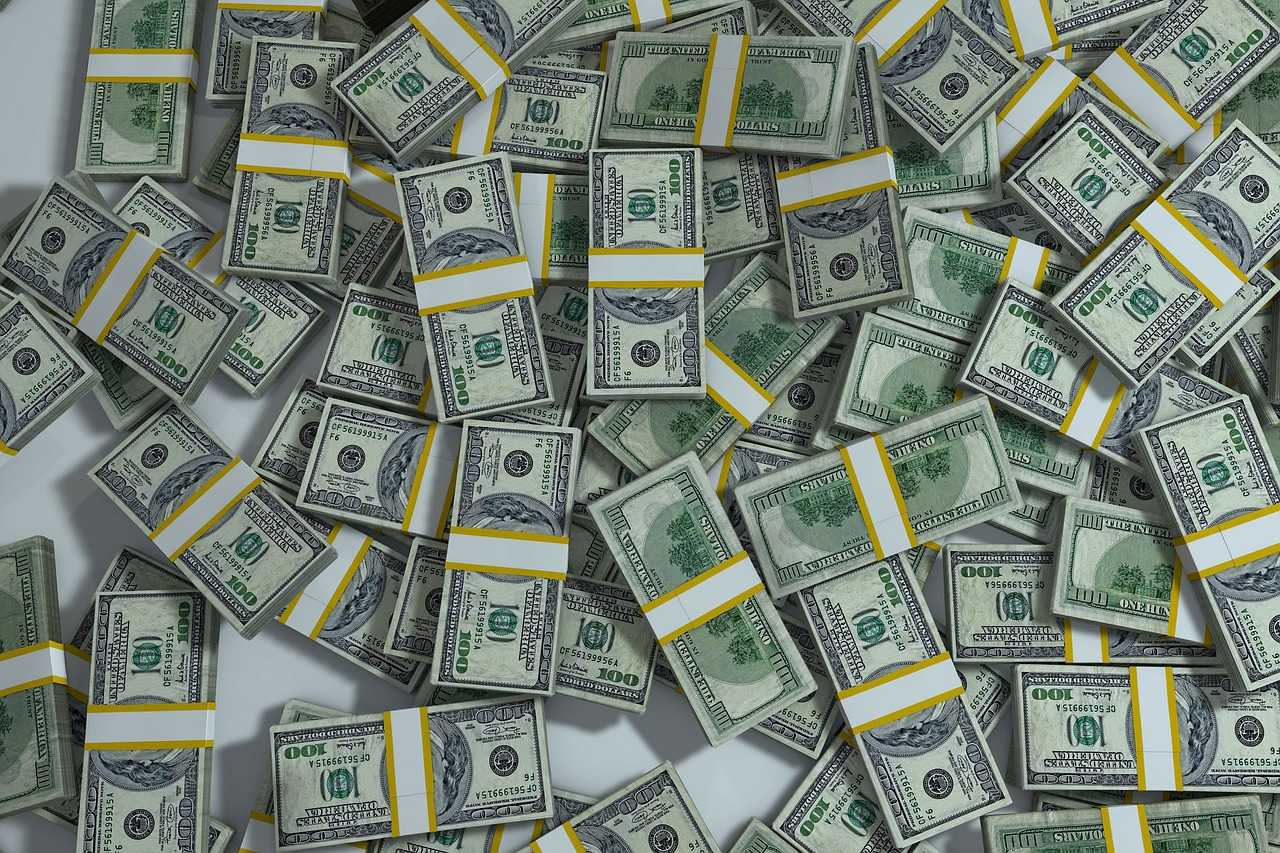
\includegraphics[scale=0.07]{MoneyPile1}}Your goal would be to make more money than you took out as a loan; that way, when you pay back the loan, you'll have a little left over to pay your employees and yourself.

\paragraph{Time Value} We say then that money has \textit{time value}, meaning that if I have a certain pile of money, I expect it to grow over time if I use it properly.  Since everyone treats money this way, if I want to borrow someone else's money and use it for some time, I need to pay them back for the money that they could have made off of it.  This is where \textit{interest} comes into play.  Interest is essentially the price we pay to use someone else's money---think of it as renting their money.  This works both ways---if I want to buy a house, I need money right now, so I borrow from a bank, but I have to, over time, pay them not only the money I borrowed, but also the money they expected to make off of it through their own investments.  Likewise, when I place my money in a bank account, the bank pays me interest in return for being able to use that money to invest and make their pile of money a bit bigger.  Thus, we talk about the \textit{present value} of money, and its \textit{future value}.  The future value is hopefully greater than the present value, since money gains value over time (assuming that inflation doesn't wipe out that gain).

Since interest is given as a rate, the amount of interest you would owe on a particular loan depends on the size of the loan (the interest is a percentage of the amount you take out).

\begin{proc}{Vocabulary}
\begin{itemize}
\item \textbf{Principal:} The amount of money that is borrowed.  This can be paid back in one lump sum, or gradually over time.
\item \textbf{Simple Interest:} Interest that is calculated based on the principal alone.
\item \textbf{Compound Interest:} Interest that is calculated based on the principal and the accumulated interest.
\end{itemize}
\end{proc}

\subsection{Simple Interest}
Suppose you take out a loan for \$500 at 10\% annual interest rate for 4 years.  Each year, (\$500)(0.1) = \$50 in interest accrues, so the total interest is 4 times this:
\[(\$500)(0.1)(4) = \$200\]
At the end of the 4 years, you'll have to pay back the principal, \$500, plus the interest, \$200, for a total of \$700, so a present value of \$500 grew to a future value of \$700.  Clearly, this growth depends on the interest rate and the amount of time involved.

\begin{formula}{Simple Interest}
The interest, $I$, earned on a loan with principal $P$ at annual interest rate $r$ (expressed as a decimal) over a period of $t$ years is
\[I=Prt\]
This formula works with other time periods (months, for instance) as long as the interest rate is given in the same terms (so a monthly interest rate, for instance).

\paragraph{Future Value}
The future value ($F$) of this principal (or present value) $P$ is the sum of the principal and the interest:
\begin{align*}
F &= P + Prt\\
F \marginnote{Future value for simple interest}&= P(1+rt)
\end{align*}
Other kinds of loans (like compound interest) will have different formulas for future value, but the principal is the same: this formula tells how this money will grow.
\end{formula}

\paragraph{APR: Annual Percentage Rate} Note carefully that $t$ is measured in \textit{years}; this is consistent for almost all the financial formulas in this chapter.  This means that interest rates are given as \textit{annual} interest rates.  It's also possible to express loans in monthly terms.  To do so, the APR is divided into a monthly interest rate; for example, a 12\% APR would be 1\% monthly, a 6\% APR would be 0.5\% monthly, etc.

\begin{example}[https://www.youtube.com/watch?v=TJqhAMb2T6Q]{Simple Interest}
\marginnote{\includegraphics[scale=0.15]{TNote1}}
Treasury notes and savings bonds are issued by the federal government to cover its expenses and debt.
Suppose you obtain a \$1,000 Series EE savings bond with a 4\% annual rate and sell it 8 years later. How much interest will you earn?\\
\vspace{0.2in}

\marginnote{\bfseries Solution}
Use the simple interest formula above:
\begin{align*}
I &= Prt\\
&= (\$1000)(0.04)(8)\\
&= \$320
\end{align*}

You'll earn \$320 in interest, so at the end you'll have a total of \$1320.
\end{example}

\begin{try}[http://izzomath.com/103text/finance/example3.1/story.html]
You deposit \$3000 in a savings account at BB\&T Bank, earning 5\% interest.  Find the amount of interest earned and the total amount in the account after three years.
\end{try}

\begin{example}[https://www.youtube.com/watch?v=T4BcmTGwJCI]{Future Value with Simple Interest}
If you deposit \$6200 at 6\%, what is the future value of the deposit at the end of 2.5 years?\\

\marginnote{\bfseries Solution}
Rather than calculating the interest first and adding that onto the principal, we can use the future value formula to do both steps at once:
\begin{align*}
F &= P(1+rt)\\
&= \$6200(1+(0.06)(2.5))\\
&= \$7130
\end{align*}
\end{example}

\begin{try}[http://izzomath.com/103text/finance/example3.2/story.html]
What is the future value of \$2400 at 7\% simple interest at the end of three years?
\end{try}

\begin{example}[https://www.youtube.com/watch?v=0GFzH0JPYeY]{Present Value with Simple Interest}
You'd like to buy a \$12,000 car in 18 months, and your bank is offering 6\% simple interest.  How much should you deposit now in order to have a final balance of \$12,000?\\

\marginnote{\bfseries Solution}
\marginnote{\includegraphics[scale=0.15]{VWVan1}}
We can use the same future value formula as in the previous example, but now the future value is given, and the present value is the unknown part:
\begin{align*}
F &= P(1+rt)\\
\$12,000 &= P(1+(0.06)(1.5))\\
\end{align*}
Now solve this for $P$ to find the amount that you need to deposit today:
\begin{align*}
\$12,000 &= P(1.09)\\
\dfrac{\$12,000}{1.09} &= P = \$11,009.17
\end{align*}
You'll need to deposit \$11,009.17 today in order to have \$12,000 in the account in 18 months.
\end{example}

\begin{try}[http://izzomath.com/103text/finance/example3.3/story.html]
How much do you need to deposit today in an account earning 3\% simple interest to have \$800 in 36 months?
\end{try}

\subsection{Compound Interest}
With simple interest, we assumed that we pocketed the interest when we received it.  If, on the other hand, we added that interest to the account, we could earn interest on that interest in the future, making the balance grow a little bit faster.  This reinvestment of interest is called \textbf{compounding}.\\

Suppose we deposit \$5000 for 5 years in an account offering an 8\% APR, with interest compounded yearly.  How much will be in the account at the end?

At the end of each year, 8\% of the balance at that point will be added to the account, and the balance will grow.  The following table shows on a year-to-year basis the total dollar amount in the account at the end of each year and the interest that accrues that year.
\begin{center}
\begin{tabular}{| c | p{1in} | p{1.52in} | p{1.5in} |}
\hline
{\small Year} & {\small Starting Balance} & {\small Interest Earned} & {\small Final Balance}\\
\hline
1 & \$5000 & $\$5000 \times 0.08 = \$400$ & $\$5000 + \$400 = \$5400$\\
\hline
2 & \$5400 & $\$5400 \times 0.08 = \$432$ & $\$5400 + \$432 = \$5832$\\
\hline
3 & \$5832 & $\$5832 \times 0.08 = \$467$ & $\$5832 + \$467 = \$6299$\\
\hline
4 & \$6299 & $\$6299 \times 0.08 = \$504$ & $\$6299 + \$504 = \$6803$\\
\hline
5 & \$6803 & $\$6803 \times 0.08 = \$544$ & $\$6803 + \$544 = \$7347$\\
\hline
\end{tabular}
\end{center}
The total amount in the account at the end of the fifth year is \$7347, which is \$347 more than we would have earned using simple interest.  Notice that each year, the amount of interest that we earned grew, making the account grow faster and faster.  This is the advantage of compounding, and over long periods of time it can lead to very dramatic results.\\

Following this example, we can derive a formula to take care of the calculation for us so that we don't have to build a table like this every time.  At the end of the first year, the balance had grown to \[\$5000+(\$5000)(0.08) = \$5000(1+0.08).\]  Following the pattern, each year the balance is multiplied by $(1+0.08)$, so at the end of the second year, the balance grew to 
\[\$5000(1+0.08)(1+0.08) = \$5000(1+0.08)^2.\]  At the end of the third year, then, the account would hold $\$5000(1+0.08)^3$, and so on.

After $t$ years, the amount in an account with an interest rate of $r$, compounded once per year, will be\marginnote{Future value for interest compounded yearly} \[F=P(1+r)^t\]

\paragraph{What if interest isn't compounded yearly?} The formula we just derived assumes that interest is compounded---or added to the account---at the end of each year.  However, this doesn't have to be the case; interest could be compounded twice a year (semiannually), four times a year (quarterly), monthly, weekly, or even daily.  \marginnote{\begin{tabular}{r | l}
{\small Compounded} & $n$\\
\hline
{\small Annually} & 1\\
{\small Semiannually} & 2\\
{\small Quarterly} & 4\\
{\small Monthly} & 12\\
{\small Weekly} & 52\\
{\small Daily} & 365\footnotemark
\end{tabular}}\footnotetext{Before calculators were commonplace, some calculations used $n=360$ for daily compounding to make the arithmetic simpler} keep track of how often interest is compounded, we define $n$ as the \textbf{number of times per year that interest is compounded}, regardless of how many years the account grows.

Now if we split the year into $n$ segments, the interest rate will be divided up as well, so each segment will earn an interest rate of $\frac{r}{n}$, so that will replace $r$ in the compound interest formula.  Also, rather than having the interest accrue $t$ times, it will accrue $n$ times each year for $t$ years, or a total of $nt$ times, so that will replace $t$ in the compound interest formula.
\vspace{0.5in}

All of this brings us to the complete formula for the future value of an investment with compound interest.
\begin{formula}{Compound Interest}
The future value $F$ of a principal amount $P$ with an annual interest rate $r$ (expressed as a decimal) compounded $n$ times per year for $t$ years is
\[F=P\left(1+\dfrac{r}{n}\right)^{nt}\]
Notice that if interest is compounded yearly, $n=1$, and the formula becomes the one we derived after the example above.
\end{formula}
\vfill

\begin{example}[https://www.youtube.com/watch?v=UCQJgC0nRxA]{Certificate of Deposit}
A certificate of deposit (CD) is an account that many banks offer that often comes with a higher interest rate, but the investment cannot be touched for a specified length of time.  Suppose you deposit \$3000 in a CD earning 6\% interest compounded monthly.  How much will you be able to withdraw at the end of 20 years?\\

\marginnote{\bfseries Solution}
List the pieces of the formula that are given:
\begin{center}
\begin{tabular}{l l}
$P$ & \$3000\\
$r$ & 0.06\\
$n$ & 12\\
$t$ & 20
\end{tabular}
\end{center}
So at the end of the 20 years, the account will hold 
\[F = 3000\left(1+\dfrac{0.06}{12}\right)^{(12)(20)} = \$9930.61\]

Now compare this to the amount you would earn from simple interest.
\begin{center}
\begin{tabular}{l | r | r}
Years & Simple Interest & Compound Interest\\
\hline
5 & \$3900 & \$4046.55\\
10 & \$4800 & \$5458.19\\
15 & \$5700 & \$7362.28\\
20 & \$6600 & \$9930.61\\
25 & \$7500 & \$13,394.91\\
30 & \$8400 & \$18,067.73\\
35 & \$9300 & \$24,370.65
\end{tabular}
\end{center}
\pagebreak

\begin{center}
\begin{tikzpicture}
\begin{axis}[
    xmin=0, xmax=40,
    ymin=0, ymax=30,
    axis lines=center,
    axis on top=false,
    domain=0:1,
    x=0.26cm,
    y=0.26cm,
    xtick={5,10,...,35},
    xticklabels={5,10,...,35},
    ytick={0,5,...,25},
    yticklabels={0,{5,000},{10,000},{15,000},{20,000},{25,000},{30,000}},
    axis lines=middle,
    axis line style={->},
    x label style={at={(axis description cs:0.5,-0.1)},anchor=north},
    y label style={at={(axis description cs:-0.15,.5)},rotate=90,anchor=south},
    xlabel={Years},
    ylabel={Account Balance (\$)},
    grid=major
    ]
	\addplot [blue,only marks] table {
	5 3.9
	10 4.8
	15 5.7
	20 6.6
	25 7.5
	30 8.4
	35 9.3
	};
	\addplot [blue,ultra thick] table {
	5 3.9
	10 4.8
	15 5.7
	20 6.6
	25 7.5
	30 8.4
	35 9.3
	};
	\addplot [green!50!black,only marks] table {
	5 4.047
	10 5.548
	15 7.362
	20 9.931
	25 13.395
	30 18.068
	35 24.371
	};
	\addplot [green!50!black,ultra thick] table {
	5 4.047
	10 5.548
	15 7.362
	20 9.931
	25 13.395
	30 18.068
	35 24.371
	};
\end{axis}
\end{tikzpicture}
\end{center}
%\includegraphics[scale=0.65]{SimpleCompoundGraph}
%\end{center}
This illustrates the difference between the linear growth offered by simple interest and the exponential growth offered by compound interest.  Over a long period of time, compounding makes a huge difference.
\end{example}

\begin{proc}{Using Your Calculator: Exponents}
\begin{tabular}{c l}
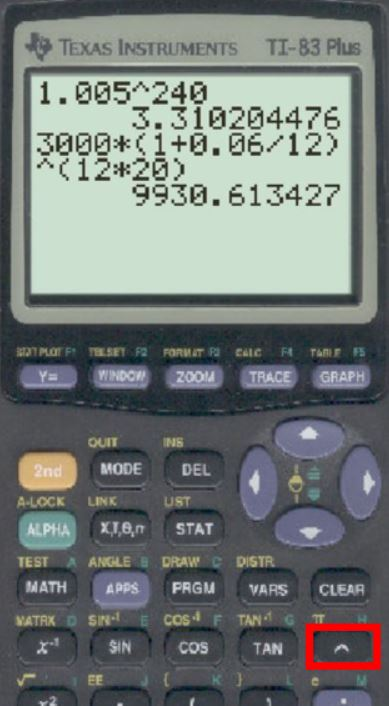
\includegraphics[scale=0.35]{Calculator1} & \parbox[b]{3in}{To evaluate an exponent like $1.005^{240}$ we use the exponent key like the one shown, or possibly $\boxed{y^x}$ or $\boxed{x^y}$ on some calculators.\\  Be careful when evaluating these often-complicated financial formulas; it's usually safer to evaluate them in pieces, like in the first line, where we began by calculating $1+0.06/12 = 1.005$ and $(12)(20)=240$, and then using the exponent key.  If you want to evaluate the entire formula in one step, be careful to use parentheses to do each operation in the proper order, as shown in the second line.\\  Also, be very careful with rounding; keep at least three significant digits (digits after leading zeros) from one calculation to the next, or use the calculator storage function.}
\end{tabular}
\end{proc}

\begin{try}[http://izzomath.com/103text/finance/example3.4/story.html]
If you deposit \$700 at 5\% interest compounded monthly, how much will the account hold in 13 years?
\end{try}
\vfill
\pagebreak

Just like with simple interest, we can use the compound interest formula to answer questions about the present value needed to obtain a given future value.

\begin{example}[https://www.youtube.com/watch?v=pT9iEqWwQ-g]{Saving for College}
You know that you will need \$40,000 for your child's education in 18 years.  If your account earns 4\% compounded quarterly, how much would you need to deposit now to reach your goal?\\

\marginnote{\bfseries Solution}
List the pieces of the formula that are given:
\begin{center}
\begin{tabular}{l l}
$F$ & \$40,000\\
$r$ & 0.04\\
$n$ & 4\\
$t$ & 18
\end{tabular}
\end{center}
In this example, $F$ is given and $P$ is unknown:
\[40,000 = P\left(1+\dfrac{0.04}{4}\right)^{(12)(18)}\]
Solve for $P$:
\[P=\dfrac{40,000}{\left(1+\dfrac{0.04}{4}\right)^{(12)(18)}}=\$19,539.84\]
\end{example}

\begin{try}[http://izzomath.com/103text/finance/example3.5/story.html]
If you want to have \$26,000 in a college fund in 12 years, and you find an account earning 5\% compounded daily, how much should you deposit now?
\end{try}

\begin{proc}{Using Your Calculator: Avoid Rounding If You Can}
In many cases, you can avoid rounding to make your answers more precise based on how you use your calculator.  For example, to calculate something like
\[F = 1000\left(1+\dfrac{0.05}{12}\right)^{(12)(30)}\] start from the inside and work outward.  We can quickly calculate (maybe even mentally) that $(12)(30) = 360$, and now we can use the calculator:
\begin{center}
\begin{tabular}{c | c}
\textbf{Type This} & \textbf{Calculator Shows}\\
\hline
& \\
0.05 $\boxed{\div}$ 12 $\boxed{=}$ & 0.00416666666667\\
& \\
$\boxed{+}$ 1 $\boxed{=}$ & 1.00416666666667\\
& \\
$\boxed{y^x}$ 360 $\boxed{=}$ & 4.46774431400613\\
& \\
$\boxed{\times}$ 1000 $\boxed{=}$ & 4467.74431400613
\end{tabular}
\end{center}
\end{proc}
\pagebreak

\begin{example}[https://www.youtube.com/watch?v=o_iz3lt-GiU]{Don't Round Too Much}
To see why not over-rounding is so important, suppose you were investing \$1000 at 5\% compounded monthly for 30 years.
\begin{center}
\begin{tabular}{l l}
$P$ & \$3000\\
$r$ & 0.06\\
$n$ & 12\\
$t$ & 20
\end{tabular}
\end{center}
To use the formula, we'll need $\frac{r}{n}$, which is 0.0041666666666$\ldots$\\

Notice the effect of rounding this to different values:
\begin{center}
\begin{tabular}{l l l}
$r/n$ rounded: & Gives $F$ to be: & Error\\
\hline
No rounding & \$4467.74 & \\
0.0041667 & \$4467.80 & \$0.06\\
0.004167 & \$4468.28 & \$0.54\\
0.00417 & \$4473.09 & \$5.35\\
0.0042 & \$4521.45 & \$53.71\\
0.004 & \$4208.59 & \$259.15
\end{tabular}
\end{center}
Notice that the error grew by \textit{about} a factor of 10 each time, which is not unusual, considering that we rounded off a digit each time.  

For our purposes, the answer we got by rounding to 0.004167 (four significant digits) is good enough - as long as we're not working in a bank, a rounding error of \$0.54 is fine for us.
\end{example}

\subsection{Comparing Interest Rates}
\begin{example}[https://www.youtube.com/watch?v=8xqmxdrDOcQ]{Comparing Banks}
\marginnote{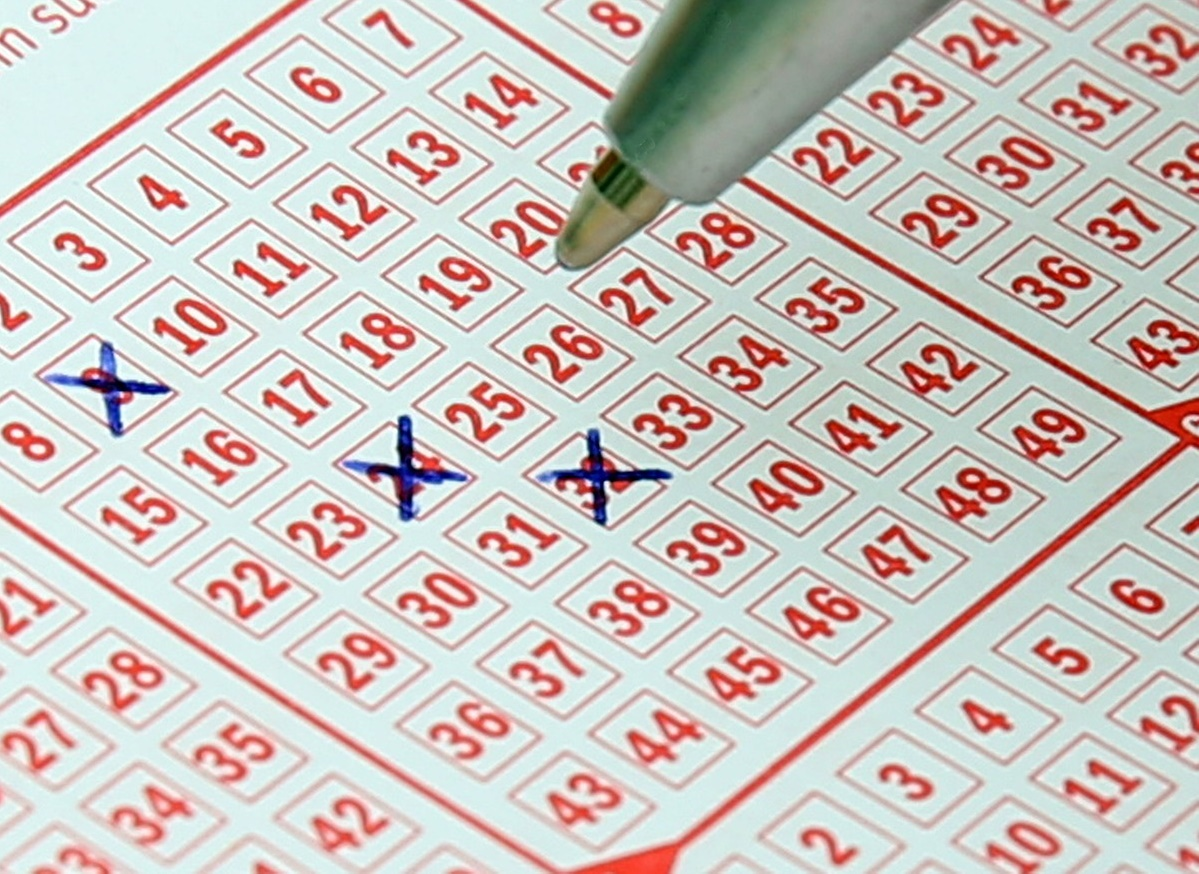
\includegraphics[scale=0.1]{Lottery1}}
You have just won \$500 in the Daily Pick 3 lottery and you decide to deposit your winnings in the bank.  You check with two different banks, which offer different options.  M\&T Bank offers a 4.25\% interest rate compounded daily, while SunTrust offers 4.3\% compounded annually.  Which bank should you choose?\\

\marginnote{\bfseries Solution}
To compare the two banks, simply choose an arbitrary amount of time and calculate how much each account would hold at the end of that time; whichever is higher is the one you'll choose.  Let's pick a year as our length of time, just for simplicity.  The table below shows the results of calculating the future value of your \$500 at the end of a year with each bank.
\begin{center}
\begin{tabular}{c c}
M\&T & SunTrust\\
\hline
& \\
\$521.71 & \$521.50
\end{tabular}
\end{center}
Even though the difference is relatively small, you'll choose the first account, since over time the difference may grow to something more significant.
\end{example}

That example illustrates an important point: you'll often find different loans or accounts expressed in different terms, perhaps with different interest rates and compounding periods.  In that case, you'll want to find some way to put them all on equal footing to compare them; like we did in this example, you can often do a quick calculation to see which will earn more in some arbitrary amount of time.

Banks will often take advantage of the financial illiteracy of their clients to present a loan in terms that will subtly benefit them.  The major goal of this chapter is to turn you into a financially literate and savvy consumer.
\vfill
\pagebreak

\paragraph{Nominal Interest Rate} The \textit{nominal interest rate} is the interest rate that is stated, such as a 3\% annual rate on a bond or a 1.7\% monthly rate on a credit card.

\paragraph{Annual Percentage Rate (APR)} This is the annual nominal rate.  So for instance, the 1.7\% nominal monthly rate would correspond to a $1.7\% \times 12 = 20.4\%$ APR.

\paragraph{Effective Interest Rate} This is the real interest rate.  The \textit{effective rate}, also called the \textit{annual percentage yield (APY)} or the \textit{effective annual yield}, takes the compounding period into account.  This is done by calculating the simple interest rate that would lead to the same growth as that of the compound interest that is offered.\\

In case that's not confusing enough, this doesn't even take into account inflation, or what the rest of the market is doing in general, which are important considerations when investing.

\begin{example}[https://www.youtube.com/watch?v=mkUrRp9le-8]{Calculating the Effective Interest Rate}
You find an account offering 6\% compounded monthly.  What is the effective annual rate?\\

\marginnote{\bfseries Solution}
To find the APY, pick an arbitrary amount of money, and track what the account does for one year.  Let's use \$1000, since it's a nice round sum.  At the end of one year, the account will hold
\[F=\$1000\left(1+\dfrac{0.06}{12}\right)^{(12)(1)} = \$1061.68\]
\paragraph{APY} Now, we need to figure out what interest rate, using simple interest, would make \$1000 grow to \$1061.68 in one year:
\begin{align*}
F &= P(1+rt)\\
1061.68 &= 1000(1+(r)(1))\\
1.06168 &= 1+r\\
0.06168 &= r
\end{align*}
The APY on this account is 6.168\%.
\end{example}

\begin{try}[http://izzomath.com/103text/finance/example3.8/story.html]
If an account offers an APR of 5\% compounded weekly, what is the effective annual interest rate?
\end{try}

\paragraph{APR vs APY} Since APY takes the effect of compounding into account and APR does not, the APY will be slightly higher than the APR for a typical account.  Because of this, banks typically report the APR for debt-related accounts like credit cards and mortgages, and they report the APY for interest-bearing accounts like CDs and money market accounts.\\

Rather than using the procedure in the example above to calculate effective interest rates, we can use a formula to accomplish the same calculation in one step.  It's important to understand, though, that this formula is nothing new; it does exactly what we did in that example, but it does it more quickly.  Thus, if you don't have the formula handy, you can still calculate the effective interest rate as long as you remember that it means the simple interest rate that will lead to the same growth as the compound one after a single year.

\begin{formula}{Effective Annual Yield}
If\marginnote{Using the formula with the numbers from the previous example: \begin{align*}
APY &= \left(1+\dfrac{0.06}{12}\right)^{12}-1\\
&= (1.005)^{12}-1 \\
&= 0.06168
\end{align*}} an account has a nominal annual interest rate of $r$, in decimal form, compounded $n$ times per year, then the effective annual yield, or APY, is given by the following formula.
\[APY = \left(1+\dfrac{r}{n}\right)^n - 1\]
\end{formula}
\vfill
\pagebreak

\begin{example}[https://www.youtube.com/watch?v=P9XX9m4UTdI]{Calculating APY}
A CD offers a nominal interest rate of 4.5\% compounded monthly.  What is the APY for this CD?\\

\marginnote{\bfseries Solution}
Here $r = 0.045$ and $n=12$:
\[APY = \left(1+\dfrac{0.045}{12}\right)^{12} - 1 = 0.04594\]
so the APY is 4.594\%.
\end{example}

\begin{try}[http://izzomath.com/103text/finance/example3.9/story.html]
The APR on a mortgage is 2.83\% compounded monthly.  What is the APY for this mortgage?
\end{try}

\subsection{Continuously Compounded Interest}
We've seen that compound interest makes money grow faster than simple interest does, but we can go even further: if someone offered you an investment compounded monthly and one compounded daily (with everything else equal), which would you choose?  You would be wise to choose the one that is compounded daily, because the more frequently that interest is compounded, the longer that interest that is added has to grow.  In other words, the interest that is added after one day has more time to grow than if it had to wait until the end of the month to be added.

The question is this: is there a limit to this growth?  Could we compound more and more often and see our money grow infinitely?  To answer this, suppose we deposit \$1 for one year into an account with a fixed interest rate---we'll use 100\% to illustrate, even though you'll almost certainly never encounter such an interest rate in real life---and we'll see what happens as we increase $n$, the frequency with which the interest is compounded:
\begin{center}
\begin{tabular}{r r}
$n$ & \hspace{0.5in} $1\left(1+\dfrac{1}{n}\right)^n$\\
\hline
1 & 2.0000000$\ldots$\\
5 & 2.4883200$\ldots$\\
10 & 2.5937424$\ldots$\\
50 & 2.6915880$\ldots$\\
100 & 2.7048138$\ldots$\\
1000 & 2.7169239$\ldots$\\
10,000 & 2.7181459$\ldots$\\
100,000 & 2.7182682$\ldots$\\
1,000,000 & 2.7182804$\ldots$\\
10,000,000 & 2.7182816$\ldots$\\
\end{tabular}
\end{center}

Notice that as we compound more and more frequently, we start to approach a limit.  This limit happens to be a very important number, so important that the letter $e$ is reserved for it.  It forms the basis of exponential growth, which has applications in every field of applied mathematics.\\

For a general interest rate $r$, $\left(1+\dfrac{r}{n}\right)^{nt}$ approaches $e^{rt}$ as the compounding increases.  This is what we call \textit{continously compounded interest}.

\begin{formula}{Continuous Compound Interest}
A present value $P$ will grow to a future value of $F$ under continuous compounding at an interest rate of $r$ according to:
\[F = Pe^{rt}\]
\end{formula}

\begin{proc}{Using Your Calculator: $e$}
\begin{tabular}{c l}
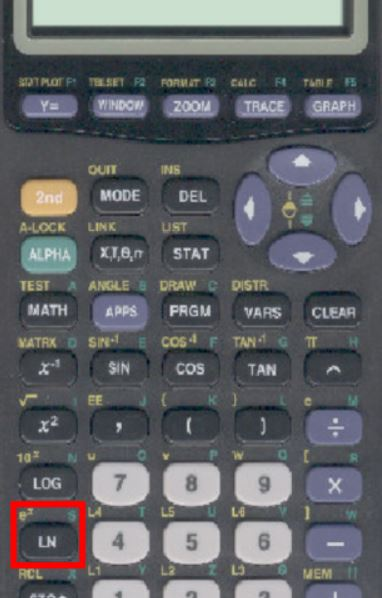
\includegraphics[scale=0.35]{CalculatorE} & \parbox[b]{3in}{Your calculator will most likely have a button for $e$, but depending on what kind of calculator you have, it may look different.\\

Here, the model shown has $e^x$ as the 2nd function of the button marked $\boxed{\textrm{LN}}$\ , so to calculate $e^{0.5}$, for instance, you would press $\boxed{\textrm{2nd}}$\ , then $\boxed{\textrm{LN}}$\ , then enter 0.5, and you should get 1.648721271.\\

On some scientific calculators, you may need to enter 0.5 and then press the $\boxed{e^x}$ key to get the same result.}
\end{tabular}
\end{proc}

\begin{example}[https://www.youtube.com/watch?v=kfZ-xUCgLl8]{Continuous Compound Interest: Future Value}
If you deposit \$4500 in an account paying 3.2\% interest compounded continuously, how much will the account hold after 36 months?\\

\marginnote{\bfseries Solution}
Use the continuous compound formula:
\[F=Pe^{rt} = \$4500e^{(0.032)(3)} = \$4953.42\]
\end{example}

\begin{try}[http://izzomath.com/103text/finance/example3.10/story.html]
If you deposit \$13,000 in an account paying 2.8\% interest compounded continuously, how much will the account hold after 3 years?
\end{try}

Just like we did with other loans, we can also calculate the present value for a given future value.

\begin{example}[https://www.youtube.com/watch?v=vzk6AvZS3h8]{Continuous Compound Interest: Present Value}
How much will you need to deposit today at 5.3\% compounded continuously in order to have \$6300 in 4 years?\\

\marginnote{\bfseries Solution}
Just like before, we'll use the same formula, but now $F$ is known and $P$ is the unknown part.
\begin{align*}
F &= Pe^{rt}\\
\$6300 &= Pe^{(0.053)(4)}\\
\$6300 &= P(1.2361)\\
\dfrac{\$6300}{1.2361} &= P\\
\$5096.48 &= P
\end{align*}
\end{example}

\begin{try}[http://izzomath.com/103text/finance/example3.11/story.html]
How much will you need to deposit today at 3.6\% compounded continuously in order to have \$1200 in 5 years?
\end{try}
\vfill
\pagebreak

\begin{example}[https://www.youtube.com/watch?v=OuC95ArdH5g]{Comparing Different Compounding Periods}
You have \$7000 to invest for 5 years.  Find how much you'll have at the end of the 5 years if you earn 4\% compounded
\begin{enumerate}[(a)]
\item annually
\item monthly
\item daily
\item continuously
\end{enumerate}
\vspace{0.2in}

\marginnote{\bfseries Solution}
The first three all use the same formula, and all that changes is $n$:
\begin{enumerate}[(a)]
\item Compounded annually:
\begin{align*}
F &= P\left(1+\dfrac{r}{n}\right)^{nt}\\
&= 7000\left(1+\dfrac{0.04}{1}\right)^{(1)(5)}\\
&= \$8516.57
\end{align*}

\item Compounded monthly:
\begin{align*}
F &= P\left(1+\dfrac{r}{n}\right)^{nt}\\
&= 7000\left(1+\dfrac{0.04}{12}\right)^{(12)(5)}\\
&= \$8546.98
\end{align*}

\item Compounded daily:
\begin{align*}
F &= P\left(1+\dfrac{r}{n}\right)^{nt}\\
&= 7000\left(1+\dfrac{0.04}{365}\right)^{(365)(5)}\\
&= \$8549.73
\end{align*}

\item Compounded continuously:
\begin{align*}
F &= Pe^{rt}\\
&= 7000e^{(0.04)(5)}\\
&= \$8549.82
\end{align*}
\end{enumerate}
\end{example}

\begin{try}[http://izzomath.com/103text/finance/example3.12/story.html]
If you deposit \$300, how much will you have in 7 years if you receive 3.5\% interest compounded
\begin{enumerate}[(a)]
\item quarterly?
\item monthly?
\item weekly?
\item continuously?
\end{enumerate}
\end{try}
\vfill
\pagebreak

\paragraph{Doubling Time} One common measure used to quickly compare investments is to determine how long it will take to double an investment.  The shorter the doubling time, the better the investment.

\begin{proc}{Solving Exponential Equations}
To solve an exponential equation, we use logarithms.  For exponential equations, we'll use the \textit{natural logarithm}, $\ln$.
\[\textrm{If } e^x = y, \textrm{ then } x = \ln y\]
\end{proc}

We can use this to solve equations where we know the present value, and we want to find the amount of time to reach a given future value.  Once we get to \[\dfrac{F}{P}=e^{rt}\] we'll use the natural logarithm to extract the exponent $rt$:
\[\ln \dfrac{F}{P} = rt\]

Since we can evaluate the expression on the left with a calculator, we can get an answer for $t$, the amount of time it will take for $P$ dollars to grow to $F$ dollars.

\begin{example}[https://www.youtube.com/watch?v=WKByWayHv00]{Doubling Time}
Find the time required to double an investment at 6\% interest compounded continuously.\\

\marginnote{\bfseries Solution}
We could again pick an arbitrary amount for $P$, and let $F$ be double that.  Instead, though, we'll simply replace $F$ with $2P$, and solve the formula for $t$:
\begin{align*}
F &= Pe^{rt}\\
2P &= Pe^{0.06t}\\
2 &= e^{0.06t}\\
\ln 2 &= 0.06t\\
\dfrac{\ln 2}{0.06} &= t\\
11.55 &= t
\end{align*}
Thus the investment will take approximately 11.5 years to double.
\end{example}

\begin{try}[http://izzomath.com/103text/finance/example3.13/story.html]
How long will it take an investment to double at 5\% compounded continuously?
\end{try}

\begin{proc}{Doubling Time}
A quick back-of-the-envelope way to approximate doubling time is to divide 72 by the percent interest rate (i.e. not the decimal form, but 100 times that).  So for example, with an interest rate of 6\%:
\[\textrm{Doubling Time } \approx \dfrac{72}{6} = 12\]
\end{proc}
\pagebreak

\subsection{Inflation}
During inflation, prices increase.  While this growth is usually not constant, if we approximate short periods of inflation as increasing at a constant rate, we can use the compound interest formula to model it.

\begin{example}[https://www.youtube.com/watch?v=gNp9Dlq-ksk]{Inflation}
Suppose that there is constant 4\% inflation from mid-2015 through mid-2020.  What will the projected price be in mid-2020 for an item that costs \$150 in mid-2015?\\

\marginnote{\bfseries Solution}
Use the compound interest formula with $P=\$150$, $r=0.04$, $n=1$, and $t=5$:
\[F=\$150\left(1+\dfrac{0.04}{1}\right)^{(1)(5)} = \$182.50\]
\end{example}

\begin{try}[http://izzomath.com/103text/finance/example3.14/story.html]
If there is constant 3\% inflation from 2015 to 2018, what will a \$85 item in 2015 cost in 2018?
\end{try}

Inflation can also be thought of as a depreciating dollar; in other words, a dollar will buy less next year than it buys now.  It turns out we can still use the compound interest formula, but now the ``interest rate''---actually the rate of depreciation---is negative.

Suppose, for illustration, that inflation is 25\%.  What costs \$100 today will cost \$125 in a year, so a dollar will only buy 80\% of what a dollar can buy today (\$100/\$125).  Thus, the depreciation rate is 20\%.  In general, if $i$ is the rate of inflation, the rate of depreciation (taken as negative) is
\[d=\dfrac{i}{1+i}.\]

Therefore, to calculate the future value of a dollar under inflation, we can use the compound interest formula with $n=1$ and $r=-\dfrac{i}{1+i}$:
\[F=P\left(1-\dfrac{i}{1+i}\right)^t\]

\begin{example}[https://www.youtube.com/watch?v=bNXuphP1Yc4]{Depreciating Dollars}
If there is constant 4\% inflation from mid-2015 through mid-2020, what will the value of a 2020 dollar be in terms of 2015 dollars?\\

\marginnote{\bfseries Solution}
Since inflation is occurring at 4\%, \[d=\dfrac{0.04}{1.04} = 0.03846,\] so using the compound interest formula: 
\[F=\$1(1-0.03846)^5 = \$0.82\]  Thus, a dollar in 2015 will only be worth \$0.82 five years later.
\end{example}

\begin{try}[http://izzomath.com/103text/finance/example3.15/story.html]
If there is constant 3\% inflation from 2015 to 2018, what will the value be of a 2018 dollar in terms of 2015 dollars?
\end{try}

In reality, inflation does not actually occur at a constant rate.  Thus, rather than using the compound interest formula to evaluate inflation, the US Bureau of Labor Statistics measures the cost of common goods periodically and compares the results to costs at other points in time to determine how inflation has changed the value of a dollar.  It is not a perfect system by any means, but it can give a good approximation for the value of a dollar in comparison to other years.

This process creates the Consumer Price Index (CPI), and each month the CPI is recorded; we'll use the average annual CPI for our examples.  Recently, the base years are taken as 1982-1984, so the average index for 1982-1984 is set to 100.  The table below records the CPI for each year from 1980 to 2003.
\begin{center}
\label{CPI Table}
\begin{tabular}{c r | c r | c r}
\textbf{Year} & CPI & \textbf{Year} & CPI & \textbf{Year} & CPI\\
\hline
& & & & & \\
\textbf{1950} & 24.1 & \textbf{1968} & 34.8 & \textbf{1986} & 109.6\\
\textbf{1951} & 26.0 & \textbf{1969} & 36.7 & \textbf{1987} & 113.6\\
\textbf{1952} & 26.6 & \textbf{1970} & 38.8 & \textbf{1988} & 118.3\\
\textbf{1953} & 26.7 & \textbf{1971} & 40.5 & \textbf{1989} & 124.0\\
\textbf{1954} & 26.9 & \textbf{1972} & 41.8 & \textbf{1990} & 130.7\\
\textbf{1955} & 26.8 & \textbf{1973} & 44.4 & \textbf{1991} & 136.2\\
\textbf{1956} & 27.2 & \textbf{1974} & 49.3 & \textbf{1992} & 140.2\\
\textbf{1957} & 28.1 & \textbf{1975} & 53.8 & \textbf{1993} & 144.5\\
\textbf{1958} & 28.9 & \textbf{1976} & 56.9 & \textbf{1994} & 148.2\\
\textbf{1959} & 29.1 & \textbf{1977} & 60.6 & \textbf{1995} & 152.4\\
\textbf{1960} & 29.6 & \textbf{1978} & 65.2 & \textbf{1996} & 156.9\\
\textbf{1961} & 29.9 & \textbf{1979} & 72.6 & \textbf{1997} & 160.5\\
\textbf{1962} & 30.9 & \textbf{1980} & 82.4 & \textbf{1998} & 163.0\\
\textbf{1963} & 30.6 & \textbf{1981} & 90.9 & \textbf{1999} & 166.6\\
\textbf{1964} & 31.0 & \textbf{1982} & 96.5 & \textbf{2000} & 172.2\\
\textbf{1965} & 31.5 & \textbf{1983} & 99.6 & \textbf{2001} & 177.1\\
\textbf{1966} & 32.4 & \textbf{1984} & 103.9 & \textbf{2002} & 179.9\\
\textbf{1967} & 33.4 & \textbf{1985} & 107.6 & \textbf{2003} & 184.0\\
\end{tabular}
\end{center}

To compare costs from two different years, use the ratio of the CPI in those two years:
\[\dfrac{\textrm{Cost in Year A}}{\textrm{Cost in Year B}} = \dfrac{\textrm{CPI for Year A}}{\textrm{CPI for Year B}}\]

\begin{example}[https://www.youtube.com/watch?v=tJS3kwwr8XA]{Using the CPI}
If a home cost \$190,000 in 1986, approximately what would the same home cost in 2002?\\

\marginnote{\bfseries Solution}
\marginnote{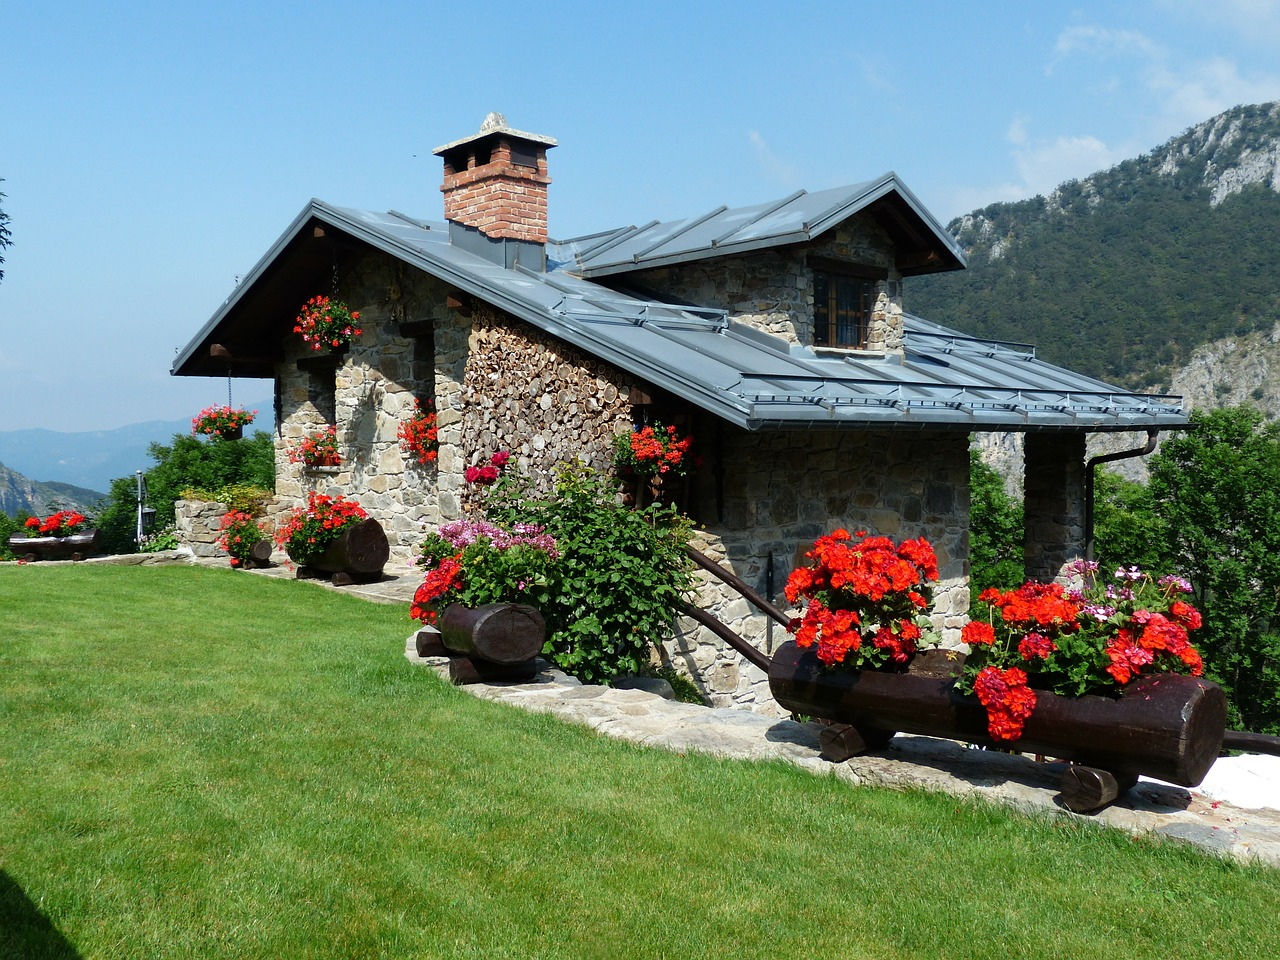
\includegraphics[scale=0.08]{House1}}
Use the proportion given above, along with the CPI table:
\begin{align*}
\dfrac{\textrm{Cost in 2002}}{\textrm{Cost in 1986}} &= \dfrac{\textrm{CPI for 2002}}{\textrm{CPI for 1986}}\\
&\\
\dfrac{\textrm{Cost in 2002}}{\$190,000} &= \dfrac{179.9}{109.6}
\end{align*}
Then, \[\textrm{Cost in 2002} = \$190,000 \times \dfrac{179.9}{109.6} \approx \$311,870\marginnote{Note: $\approx$: ``approximately''}\]
\end{example}

\begin{try}[http://izzomath.com/103text/finance/example3.16/story.html]
If a home cost \$235,000 in 1998, use the CPI table to determine how much the same home would have cost in 1978.
\end{try}

\begin{exercises}
\textit{In Exercises 1---4, a principal amount is borrowed at the given interest rate for the given period of time.  Find the loan's future value $F$, or the amount due at the end of the time, if the loan uses simple interest.}

\pfour{\begin{tabular}{r l}
Principal: & \$3000\\
Interest rate: & 7\%\\
Time: & 2 years
\end{tabular}}
\pfour{\begin{tabular}{r l}
Principal: & \$2700\\
Interest rate: & 4\%\\
Time: & 3 years
\end{tabular}}
\pfour{\begin{tabular}{r l}
Principal: & \$7500\\
Interest rate: & 3.5\%\\
Time: & 18 months
\end{tabular}}
\pfour{\begin{tabular}{r l}
Principal: & \$1600\\
Interest rate: & 4.85\%\\
Time: & 36 months
\end{tabular}}

\textit{In Exercises 5---8, a principal amount is borrowed at the given interest rate for the given period of time.  If the future value is given, find the principal if the loan uses simple interest.}

\pfour{\begin{tabular}{r l}
Future value: & \$9000\\
Interest rate: & 5.5\%\\
Time: & 1 year
\end{tabular}}
\pfour{\begin{tabular}{r l}
Future value: & \$7700\\
Interest rate: & 6\%\\
Time: & 4 years
\end{tabular}}
\pfour{\begin{tabular}{r l}
Future value: & \$800\\
Interest rate: & 2.75\%\\
Time: & 9 months
\end{tabular}}
\pfour{\begin{tabular}{r l}
Future value: & \$1450\\
Interest rate: & 5.3\%\\
Time: & 24 months
\end{tabular}}

\textit{In Exercises 9---11, a principal amount is borrowed at the given interest rate for the given period of time, and interest is compounded as stated.  Find the loan's future value $F$, or the amount due at the end of the time.}

\pthree{\begin{center}\begin{tabular}{r l}
Principal: & \$1200\\
Interest rate: & 5\%\\
Compounding: & Annually\\
Time: & 3 years
\end{tabular}\end{center}}
\pthree{\begin{tabular}{r l}
Principal: & \$5700\\
Interest rate: & 3.5\%\\
Compounding: & Monthly\\
Time: & 24 months
\end{tabular}}
\pthree{\begin{tabular}{r l}
Principal: & \$3000\\
Interest rate: & 5.32\%\\
Compounding: & Continuously\\
Time: & 48 months
\end{tabular}}

\textit{In Exercises 12---14, a principal amount is borrowed at the given interest rate for the given period of time, and interest is compounded as stated.  If the future value is given, find the principal.}

\pthree{\begin{tabular}{r l}
Future value: & \$17,500\\
Interest rate: & 3\%\\
Compounding: & Annually\\
Time: & 8 years
\end{tabular}}
\pthree{\begin{tabular}{r l}
Future value: & \$18,000\\
Interest rate: & 5.6\%\\
Compounding: & Daily\\
Time: & 18 months
\end{tabular}}
\pthree{\begin{tabular}{r l}
Future value: & \$9000\\
Interest rate: & 7.48\%\\
Compounding: & Continuously\\
Time: & 60 months
\end{tabular}}

\ptwo{A friend lends you \$200 for a week, which you agree to repay with 5\% one-time interest. How much will you have to repay?}
\ptwo{Suppose you obtain a \$3,000 T-note with a 3\% annual rate, paid quarterly, with maturity in 5 years.  How much interest will you earn?}

\ptwo{A student took out a simple interest loan for \$2,400 for two years at an annual rate of 7\%.  
\begin{enumerate}[(a)]
\item What is the interest on the loan?
\item How much will the student have to repay at the end of two years?
\end{enumerate}
}
\ptwo{A loan of \$2,040 has been made at a 5.7\% annual simple interest rate for four months.  
\begin{enumerate}[(a)]
\item What is the interest on the loan?
\item Find the future value of the loan.
\end{enumerate}}

\ptwo{You deposit \$2000 in an account earning 3\% interest compounded monthly.
\begin{enumerate}[(a)]
\item How much will you have in the account in 20 years?
\item How much interest will you earn?
\end{enumerate}}
\ptwo{You deposit \$10,000 in an account earning 4\% interest compounded weekly.
\begin{enumerate}[(a)]
\item How much will you have in the account in 25 years?
\item How much interest will you earn?
\end{enumerate}}

\ptwo{How much would you need to deposit in an account earning 6\% compounded monthly in order to have \$6,000 in the account in 8 years?}
\ptwo{How much would you need to deposit in an account earning 5\% compounded quarterly in order to have \$20,000 in the account in 4 years?}

\ptwo{If you deposit \$5400 in an account earning 4.35\% interest compounded continuously, how much will the account hold in 18 months?}
\ptwo{If you take out a loan for \$7700 at 6.7\% interest compounded continously, how much will you have to pay back in 5 years?}

\ptwo{How much do you need to deposit today at 4\% interest compounded continuously in order to have \$4000 in 2 years?}
\ptwo{If you find a CD offering 5.8\% interest compounded continuously, how much should you deposit if you are saving up to refinish your kitchen in 3 years and you estimate that will take \$15,000?}

\ptwo{If a mortgage is advertised with a 3.12\% APR, compounded monthly, what is the APY on this mortgage?  Which is the bank more likely to present to their clients?}
\ptwo{If the APR on a retirement account is 4.4\%, compounded quarterly, what is the APY?  Which is the bank more likely to advertise?}

\ptwo{You have \$12,000 to invest for 3 years.  Find how much you'll have at the end of the 3 years if you earn 4\% interest compounded
\begin{enumerate}[(a)]
\item annually
\item monthly
\item daily
\item continuously
\end{enumerate}}
\ptwo{You would like to have \$8000 saved in 3 years.  Find how much you'll have to invest now to reach that goal if you earn 6\% interest compounded
\begin{enumerate}[(a)]
\item annually
\item monthly
\item daily
\item continuously
\end{enumerate}}

\ptwo{How long will it take to double an investment at 7\% compounded annually?}
\ptwo{How long will it take to double an investment at 4.6\% compounded continuously?}

\ptwo{Suppose that there is constant 3.5\% inflation from 2015 to 2025.  What is the projected 2025 price for an item that costs \$357 in 2015?}
\ptwo{If there is constant 3.5\% inflation from 2015 to 2025, what will the value of a 2025 dollar be in terms of 2015 dollars?}

\ptwo{Use the CPI table on page \pageref{CPI Table} to estimate the cost of a gallon of milk in 1998 if it cost \$2.22 in 1986.  What percentage increase is this?}
\ptwo{Use the CPI table on page \pageref{CPI Table} to estimate the average cost of a dozen eggs in 1986 if it cost \$1.09 in 1998.  What percentage increase is this?}

\end{exercises}


\section{Annuities}
\setcounter{ExampleCounter}{1}
Suppose you're trying to save for retirement.  If you had \$500,000 today, you could invest that and perhaps in twenty years, you might have a nice retirement nest egg.  However, this isn't the situation that most of us find ourselves in---having \$500,000 in disposable cash is not in the typical American's experience.

How, then, do we save for retirement?  The answer is a \textbf{savings annuity}, which is an interest-bearing account into which we deposit regular payments.  By taking a small portion of each paycheck and depositing it into a 401(k) plan or individual retirement account (IRA), we can take advantage of the power of compounding to grow our retirement savings.  The future value of a savings annuity is the sum of all the deposits plus whatever interest accrued.

\begin{example}[https://www.youtube.com/watch?v=KOIRAWGh9vM]{Savings Annuity}
Suppose you deposit \$100 into a savings account at the end of each year.  If you earn 5\% interest compounded annually, how much will the account hold at the end of 3 years?  How much interest did the account earn?\\

\marginnote{\bfseries Solution}
At the end of the first year, the account holds the \$100 that you deposit then:
\[F_1 = \$100\]
The second year, this \$100 earns interest, plus you deposit another \$100 at the end of the year:
\[F_2 = \$100(1+0.05) + \$100 = \$205\]
The third year, this \$205 earns interest, plus you deposit another \$100 at the end of the year:
\[F_3 = \$205(1+0.05) + \$100 = \$315.25\]
We could continue this pattern indefinitely, but each year, we only need to use the simple interest formula to see how much the previous year's balance has grown, and then add in that year's deposit.\\

At the end of the three years, the account holds \$315.25, and since we deposited a total of \$300 (\$100 each year for 3 years), the account earned a total of \$15.25 in interest.
\end{example}

\subsection{Savings Annuity Formula}
In theory, we could use the procedure of the last example to calculate the value of an annuity after any length of time.  However, that process quickly gets tedious, so we'd like to have a formula instead.\\

\textit{Fair warning, though: the derivation of this formula might seem confusing, so if you'd like, you can skip down to the formula at the end.}

Suppose you deposit $P$ dollars into a savings annuity each year, and this account earns an interest rate of $r$ compounded annually (we'll handle the case of other compounding periods after we get to the formula).  At the end of the first year, the account contains $P$ dollars:
\[F_1 = P\]
This principal earns interest the second year [growing to $P(1+r)$] so at the end of the second year, the account holds that plus the newly deposited $P$:
\[F_2 = P+P(1+r)\]
Now, in the third year, this balance earns interest again: $(P+P(1+r))(1+r) = P(1+r) + P(1+r)(1+r)$, so the balance at the end of the third year is this plus another $P$:
\[F_3 = P + P(1+r) + P(1+r)^2\]
We can now see the pattern, so we can jump to the arbitrary case; at the end of $t$ years, the account will hold
\begin{equation}
F_t = P + P(1+r) + P(1+r)^2 + P(1+r)^3 + \ldots + P(1+r)^{t-1}
\end{equation}

Now comes the tricky part: we want a simpler formula for $F_t$, so we solve for it in an unexpected way.  First, multiply both sides of the last line by $(1+r)$:
\begin{equation}
F_t + F_tr = P(1+r) + P(1+r)^2 + P(1+r)^3 + \ldots + P(1+r)^{t-1} + P(1+r)^t
\end{equation}
Next, subtract equation (1.1) from equation (1.2), subtracting on both sides of the equation.  Notice that as we do so, almost all of the terms cancel:
\[F_tr = P(1+r)^t-P = P\left[(1+r)^t-1\right]\]
Finally, divide both sides of the equation by $r$ to isolate $F_t$:
\[F_t = \dfrac{P\left[(1+r)^t-1\right]}{r}\]

What if we make deposits monthly rather than yearly?  We'll assume, first of all, that the rate at which we make deposits and the rate at which interest is compounded is the same; in other words, we won't make monthly deposits to an account that compounds weekly, for instance.  If the compounding and the rate of deposit are both represented by $n$, we change this formula in the same way that we changed the compound interest formula to handle different compounding periods:
\begin{itemize}
\item Replace $r$, the annual interest rate, with $\dfrac{r}{n}$, splitting it into compounding periods.
\item Replace $t$ with $nt$ to account for the interest compounding $n$ times per year for $t$ years.
\end{itemize}
This leads to the general formula:
\[F=\dfrac{P\left[\left(1+\dfrac{r}{n}\right)^{nt}-1\right]}{\left(\dfrac{r}{n}\right)}\]

\begin{formula}{Summary: The Future Value of a Savings Annuity}
If regular deposits of $P$ are made once a year into an annuity paying an interest rate of $r$ compounded annually, the future value of the annuity at the end of $t$ years is given by
\[F = \dfrac{P\left[(1+r)^t-1\right]}{r}\]

If regular deposits of $P$ are made $n$ times per year into an annuity paying an interest rate of $r$ compounded $n$ times per year, the future value of the annuity at the end of $t$ years is given by
\[F=\dfrac{P\left[\left(1+\dfrac{r}{n}\right)^{nt}-1\right]}{\left(\dfrac{r}{n}\right)}\]

Notice that here we use $P$ to mean the amount that is regularly deposited, rather than the present value, a lump sum deposited now.
\end{formula}

Note: annuities assume that you put money in an account on a regular schedule (every month, every quarter, every year, etc.) and let it sit in the account earning interest.  This is different from basic compound interest, because that assumes that you deposit money in the account once and let it sit there earning interest.
\vfill
\pagebreak

\begin{example}[https://www.youtube.com/watch?v=X1oXL3ZjcCU]{Traditional IRA}
A traditional individual retirement account (IRA) is a retirement account in which the money you invest is tax-exempt (you can deduct your contributions on your income tax return) until you withdraw it.  Thus, taxes are deferred until you retire.  If you deposit \$100 each month into an IRA earning 6\% interest, how much will you have in the account after 20 years?\\

Organize the given information:
\begin{center}
\begin{tabular}{r l l}
$P$ & \$100 & The regular deposit\\
$r$ & 0.06 & 6\% annual rate\\
$n$ & 12 & Deposits are made monthly\\
$t$ & 20 & Deposits are made for 20 years
\end{tabular}
\end{center}

Putting it all together in the formula:
\begin{align*}
F &= \dfrac{\$100\left[\left(1+\dfrac{0.06}{12}\right)^{(12)(20)}-1\right]}{\left(\dfrac{0.06}{12}\right)}\\
&= \$46,204.09 \approx \$46,200
\end{align*}

Notice\marginnote{$(\$100)(12)(24) = \$24,000$} that you deposited \$100 every month, 12 months a year for 20 years, for a total of \$24,000.  That means that the account earned approximately $\$46,200-\$24,000 = \$22,200$ in interest.
\end{example}

\begin{try}[http://izzomath.com/103text/finance/example4.2/story.html]
If you deposit \$800 every year into a traditional IRA earning 4\% interest, how much will the account hold after 25 years?
\end{try}

%Because retirement accounts typically grow for long periods, they can experience rather dramatic growth, as seen in the last example.

There is another common type of retirement account: the Roth IRA.  The idea behind a Roth IRA was originally proposed in 1989 by Senator William Roth of Delaware and established by the Taxpayer Relief Act of 1997.

\begin{example}[https://www.youtube.com/watch?v=gqvXGP8vLxA]{Roth IRA}
In a Roth IRA, unlike a traditional IRA, you pay taxes on contributions, but when you withdraw in retirement, withdrawals are tax-free.  If you deposit \$500 every quarter into a Roth IRA earning 3.75\% interest, how much will the account hold in 30 years?\\

\marginnote{\bfseries Solution}
Organize the given information:
\begin{center}
\begin{tabular}{r l l}
$P$ & \$500 & The regular deposit\\
$r$ & 0.0375 & 3.75\% annual rate\\
$n$ & 4 & Deposits are made quarterly\\
$t$ & 30 & Deposits are made for 30 years
\end{tabular}
\end{center}

Putting it all together in the formula:
\begin{align*}
F &= \dfrac{\$500\left[\left(1+\dfrac{0.0375}{4}\right)^{(4)(30)}-1\right]}{\left(\dfrac{0.0375}{4}\right)} \approx \$110,086
\end{align*}

Notice that you deposited a total of \$60,000, which means that the account earned \$50,086 in interest, nearly as much as you deposited.
\end{example}

\begin{try}[http://izzomath.com/103text/finance/example4.3/story.html]
If you deposit \$200 every month into a Roth IRA earning 5.5\% interest, how much will the account hold after 30 years?
\end{try}
\pagebreak

The differences between traditional and Roth IRAs did not affect the calculations in the preceding examples, but we'll point them out here for the sake of the curious student.

\checkoddpage
\ifoddpage{
\begin{adjustwidth}{-0.25in}{-1.75in}
\begin{proc}{Traditional vs. Roth IRA}
The most prominent difference between traditional and Roth IRAs concerns when the contributions are taxed: traditional IRAs defer taxation until contributions are withdrawn, while Roth IRAs are taxed as contributions are made.\\

So when comparing the two, the question is this: do you expect tax rates to be higher now or when you retire?  The smart money is on tax rates increasing.  In addition to that, during retirement taxable income may be higher after the taxpayer loses the opportunity to deduct housing and education expenses and dependents are grown and gone.  Thus, Roth IRAs are popular since you can pay lower taxes now rather than deferring them until you'd have to pay more.\\

Another major difference is that traditional IRAs require you to begin withdrawing at age 70.5, while Roth IRAs have no such restriction.  Because of this, Roth IRAs can be used to transfer wealth to inheritors, since they will not have to pay income taxes on withdrawals (but perhaps estate taxes) and can stretch the withdrawals out for years.\\

The table below summarizes the comparison between traditional and Roth IRAs:
\begin{center}
\begin{tabular}{p{0.18\textwidth} | p{0.38\textwidth} p{0.38\textwidth}}
& \textbf{Traditional IRA} & \textbf{Roth IRA}\\
\hline
\textbf{2014 Contribution Limits} & \$5,500 (if under age 50) & \$5,500 (if under age 50)\\
& & \\
\textbf{2014 Income Limits} & No limits & Single tax filers with adjusted gross income of less than \$129,000; married couples filing jointly with adjusted gross income of less than \$191,000\\
& & \\
\textbf{Taxing} & Tax deduction on contribution year; ordinary income taxes owed on withdrawals & No tax break for contributions; tax-free earnings and withdrawals in retirement\\
& & \\
\textbf{Withdrawing} & Withdrawals are tax-free and penalty-free beginning at age 59.5.  Distributions must begin at age 70.5; beneficiaries pay taxes on inherited IRAs & Contributions can be withdrawn at any time, tax-free and penalty-free.  After five years and age 59.5, all withdrawals are tax-free.  No withdrawals required during account holder's lifetime.\\
\end{tabular}
\end{center}

One final note: both kinds of IRA allow first-time homebuyers to withdraw up to \$10,000 to pay for qualified housing costs.
\end{proc}
\end{adjustwidth}
} \else{
\begin{adjustwidth}{-1.75in}{-0.25in}
\begin{proc}{Traditional vs. Roth IRA}
The most prominent difference between traditional and Roth IRAs concerns when the contributions are taxed: traditional IRAs defer taxation until contributions are withdrawn, while Roth IRAs are taxed as contributions are made.\\

So when comparing the two, the question is this: do you expect tax rates to be higher now or when you retire?  The smart money is on tax rates increasing.  In addition to that, during retirement taxable income may be higher after the taxpayer loses the opportunity to deduct housing and education expenses and dependents are grown and gone.  Thus, Roth IRAs are popular since you can pay lower taxes now rather than deferring them until you'd have to pay more.\\

Another major difference is that traditional IRAs require you to begin withdrawing at age 70.5, while Roth IRAs have no such restriction.  Because of this, Roth IRAs can be used to transfer wealth to inheritors, since they will not have to pay income taxes on withdrawals (but perhaps estate taxes) and can stretch the withdrawals out for years.\\

The table below summarizes the comparison between traditional and Roth IRAs:
\begin{center}
\begin{tabular}{p{0.18\textwidth} | p{0.38\textwidth} p{0.38\textwidth}}
& \textbf{Traditional IRA} & \textbf{Roth IRA}\\
\hline
\textbf{2014 Contribution Limits} & \$5,500 (if under age 50) & \$5,500 (if under age 50)\\
& & \\
\textbf{2014 Income Limits} & No limits & Single tax filers with adjusted gross income of less than \$129,000; married couples filing jointly with adjusted gross income of less than \$191,000\\
& & \\
\textbf{Taxing} & Tax deduction on contribution year; ordinary income taxes owed on withdrawals & No tax break for contributions; tax-free earnings and withdrawals in retirement\\
& & \\
\textbf{Withdrawing} & Withdrawals are tax-free and penalty-free beginning at age 59.5.  Distributions must begin at age 70.5; beneficiaries pay taxes on inherited IRAs & Contributions can be withdrawn at any time, tax-free and penalty-free.  After five years and age 59.5, all withdrawals are tax-free.  No withdrawals required during account holder's lifetime.\\
\end{tabular}
\end{center}

One final note: both kinds of IRA allow first-time homebuyers to withdraw up to \$10,000 to pay for qualified housing costs.
\end{proc}
\end{adjustwidth}
} \fi

\begin{example}[https://www.youtube.com/watch?v=TWZhZoh9TG4]{How Much Should You Save?}
You want to have \$500,000 in your account when you retire in 35 years.  If your retirement account earns 5\% interest, how much should you deposit each month to reach your retirement goal?\\

\marginnote{\bfseries Solution}
Now everything except for $P$ is given, and that is what we are trying to determine.
\begin{center}
\begin{tabular}{r l l}
$F$ & \$500,000 & The future value\\
$r$ & 0.05 & 5\% annual rate\\
$n$ & 12 & Deposits are made monthly\\
$t$ & 35 & Deposits are made for 35 years
\end{tabular}
\end{center}

Putting it all together in the formula:
\begin{align*}
\$500,000 &= \dfrac{P\left[\left(1+\dfrac{0.05}{12}\right)^{(12)(35)}-1\right]}{\left(\dfrac{0.05}{12}\right)}\\
\$500,000 &= P(1136.092)\\
\$440.11 &= P
\end{align*}

Having\marginnote{$(\$440)(12)(35) = \$184,846.20$} half a million dollars may sound like an unattainable goal, but by making regular deposits, it becomes possible.  Notice that in this case, you'll deposit a total of \$184,846, which means that the account earns\marginnote{$\$500,000 - \$184,846 = \$315,154$} \$315,154, or close to twice the amount that you deposit.
\end{example}
\vfill
\pagebreak

\begin{try}[http://izzomath.com/103text/finance/example4.4/story.html]
You want to have \$800,000 in your account when you retire in 40 years.  If your retirement account earns 6.7\% interest, how much should you deposit each month to reach your retirement goal?
\end{try}

If there is one lesson to take away from this section, it is this: \textbf{START SAVING NOW!}  Save early and save often, and you'll be far ahead of the curve.  The next example drives this home; we'll consider two recent college graduates.  Emma learned her lesson and begins saving immediately, while Jason is overwhelmed by his expenses immediately as he begins to work and he neglects to save.  After 20 years, Jason decides to try to catch up.  Let's see how that works out (spoiler alert: Emma winds up better off).

Suppose Jason and Emma graduate the same year and begin working in adjacent cubicles; they're each 23 years old, and they'll both work for 45 years.  Let's assume that both get a 4\% interest rate in their retirement accounts. 

\begin{example}[https://www.youtube.com/watch?v=9hcZL9uCEoY]{Start Saving Early}
\begin{enumerate}[(1)]
\item If Emma begins saving \$400 every month right away and does so for 45 years, how much will her account hold when she retires?\\

Use the savings annuity formula:
\begin{align*}
F &= \dfrac{\$400\left[\left(1+\dfrac{0.04}{12}\right)^{(12)(45)}-1\right]}{\left(\dfrac{0.04}{12}\right)}\\
&\approx \$603,788
\end{align*}

\item If Jason begins saving 30 years later, and he saves \$1500 every month for 15 years, how much will his account hold when he retires?\\

Use the savings annuity formula:
\begin{align*}
F &= \dfrac{\$1500\left[\left(1+\dfrac{0.04}{12}\right)^{(12)(15)}-1\right]}{\left(\dfrac{0.04}{12}\right)}\\
&\approx \$369,136
\end{align*}
He puts away more than 3 times what Emma does each month, and yet he ends up far short of her total.

\item How much would Jason have to save each month for 15 years to match Emma's final total?\\

\begin{align*}
\$603,788 &= \dfrac{P\left[\left(1+\dfrac{0.04}{12}\right)^{(12)(15)}-1\right]}{\left(\dfrac{0.04}{12}\right)}\\
\$2454 &\approx P
\end{align*}
He'd have to save much, much more each month to catch up to Emma.

\item Compare their contributions to their final balances.
\begin{enumerate}[(a)]
\item Emma contributes a total of $\$400 \times 12 \times 45 = \$216,000$, which means that her account earned \$387,788 in interest.
\item Under Jason's first plan, he contributes \$270,000 (more than Emma, even though his final balance is much smaller), so he only earns \$99,136 in interest.
\item With Jason's modified plan where he contributes \$2454 each month, he pays in a total of \$441,720, earning \$162,068 in interest.
\end{enumerate}
\end{enumerate} 
Hopefully, the lesson is clear: start saving early!
\end{example}
\pagebreak

\subsection{Payout Annuities}
So far in this section, we've dealt with \textbf{savings annuities}, where you begin with nothing and make regular deposits that grow over time to a final balance.

The other kind is a \textbf{payout annuity}, where you begin with a lump sum and make regular withdrawals (the money remaining in the account earns interest) and the account will be empty after a fixed amount of time.  We'll be determining the amount that you should withdraw each time in order to empty the account at the right time.

Payout annuities are typically used after retirement.  Perhaps you have saved \$500,000 for retirement, and you want to take money out of the account each month for living expenses, and you want the money to last 20 years.  This is an example of a payout annuity.  Payout annuities are also often used when a large lump sum is paid out, such as with lottery winnings or lawsuit settlements.

We'll leave out the details of deriving this formula, but essentially it involves setting the amount that a lump sum will grow to according to the compound interest formula equal to the amount that is paid out using the annuity formula.  If we solve that for the lump sum (we're omitting the derivation mostly because of this step), we find the payout annuity formula below.

\begin{formula}{Payout Annuity}
If a starting balance of $P$ is paid out in regular payments of $PMT$ from an annuity earning $r$ interest compounded $n$ times per year, and the payments are made $n$ times per year, the following relationship holds:
\[P = \dfrac{PMT\left[1-\left(1+\dfrac{r}{n}\right)^{-nt}\right]}{\left(\dfrac{r}{n}\right)}\]
Notice the negative exponent; be careful when entering that into your calculator.
\end{formula}

\begin{example}[https://www.youtube.com/watch?v=A2pKYPSXUbw]{Payout Annuity}
After retiring, you want to be able to take \$1000 every month from your retirement account for 20 years.  If the account earns 6\% interest, how much will you need in your account when you retire?\\

\marginnote{\bfseries Solution}
Organize the given information:
\begin{center}
\begin{tabular}{r l l}
$PMT$ & \$500 & The regular withdrawal\\
$r$ & 0.06 & 6\% annual rate\\
$n$ & 12 & Withdrawals are made monthly\\
$t$ & 20 & Withdrawals are made for 20 years
\end{tabular}
\end{center}

Putting it all together in the formula:
\begin{align*}
P &= \dfrac{\$1000\left[1-\left(1+\dfrac{0.06}{12}\right)^{-(12)(20)}\right]}{\left(\dfrac{0.06}{12}\right)} \approx \$139,581
\end{align*}

You'll need to have approximately \$139,600 in your account when you retire.  Notice that you'll withdraw \$240,000 (\$1000 for 240 months).  You're able to pull out more than you have at retirement because you don't withdraw it all at once, but take it out little by little as you need it, allowing the remainder to earn interest before you take it out.  This difference represents \$100,400 in interest earned during those 20 years of retirement.
\end{example}

\begin{try}[http://izzomath.com/103text/finance/example4.6/story.html]
After retiring, you want to be able to take \$1500 every month from your retirement account for 15 years.  If the account earns 4.5\% interest, how much will you need in your account when you retire?
\end{try}

\begin{proc}{Calculator Note: Evaluating Negative Exponents}
With these problems, you need to raise numbers to negative powers.  Most calculators have a separate button for negating a number that is different than the subtraction button.  Some calculators label this $\boxed{(-)}$\ , and some label it $\boxed{+/-}$\ .

If your calculator has a multiline display, to calculate $1.005^{-240}$, you'd type something like $1.005 \boxed{\wedge}\ \boxed{(-)}\ 240$.

If you have a scientific calculator that only displays a single number at a time, you will most likely need to hit the $\boxed{(-)}$ key after a number to negate it.  Thus, you'd type $1.005\ \boxed{y^x}\ 240\ \boxed{(-)}\ \boxed{=}\ $.

Try it on your calculator and make sure that you get 0.302096 as your answer.
\end{proc}

Finally, let's turn this around and ask the other question: given a fixed amount in our account, how much can we withdraw in regular payments?

\begin{example}[https://www.youtube.com/watch?v=BsqVTSoWOm8]{Withdrawing from a Payout Annuity}
You expect to have \$500,000 in your IRA when you retire, and you want to be able to take monthly withdrawals for a total of 30 years.  If your account earns 8\% interest, how much will you be able to withdraw each month?\\

\marginnote{\bfseries Solution}
Organize the given information:
\begin{center}
\begin{tabular}{r l l}
$P$ & \$500,000 & The starting balance\\
$r$ & 0.08 & 8\% annual rate\\
$n$ & 12 & Withdrawals are made monthly\\
$t$ & 30 & Withdrawals are made for 30 years
\end{tabular}
\end{center}

This time we want to find $PMT$:
\begin{align*}
\$500,000 &= \dfrac{PMT\left[1-\left(1+\dfrac{0.08}{12}\right)^{-(12)(30)}\right]}{\left(\dfrac{0.08}{12}\right)}\\
\$500,000\marginnote{Note: if you don't round at this step, your answer should be \$3668.82} &= PMT(136.232)\\
\$3670.21 &= PMT
\end{align*}

You can plan to withdraw \$3670.21 each month for 30 years.
\end{example}

\begin{try}[http://izzomath.com/103text/finance/example4.7/story.html]
A donor gives \$100,000 to a university, and specifies that it is to be used to give annual scholarships for the next 20 years.  If the university can earn 4\% interest, how much can they give in scholarships each year?
\end{try}

\begin{exercises}
\textit{In Exercises 1---6, a periodic deposit is made into an annuity with the given terms.  Find how much the annuity will hold at the end of the specified amount of time.}

\pthree{\begin{center}\begin{tabular}{r l}
Regular deposit & \$250\\
Interest rate & 4\%\\
Frequency & Monthly\\
Time & 15 years\\
Future value & ?
\end{tabular}\end{center}}
\pthree{\begin{center}\begin{tabular}{r l}
Regular deposit & \$10\\
Interest rate & 5\%\\
Frequency & Daily\\
Time & 12 years\\
Future value & ?
\end{tabular}\end{center}}
\pthree{\begin{center}\begin{tabular}{r l}
Regular deposit & \$2000\\
Interest rate & 3\%\\
Frequency & Yearly\\
Time & 22 years\\
Future value & ?
\end{tabular}\end{center}}

\pthree{\begin{center}\begin{tabular}{r l}
Regular deposit & \$100\\
Interest rate & 3.75\%\\
Frequency & Weekly\\
Time & 30 years\\
Future value & ?
\end{tabular}\end{center}}
\pthree{\begin{center}\begin{tabular}{r l}
Regular deposit & \$300\\
Interest rate & 4.25\%\\
Frequency & Monthly\\
Time & 18 years\\
Future value & ?
\end{tabular}\end{center}}
\pthree{\begin{center}\begin{tabular}{r l}
Regular deposit & \$3500\\
Interest rate & 2.85\%\\
Frequency & Yearly\\
Time & 28 years\\
Future value & ?
\end{tabular}\end{center}}


\textit{In Exercises 7---12, find how much should be regularly deposited into an annuity with the given terms in order to have the specified final amount in the account.}

\pthree{\begin{center}\begin{tabular}{r l}
Regular deposit & ?\\
Interest rate & 5\%\\
Frequency & Monthly\\
Time & 18 years\\
Future value & \$50,000
\end{tabular}\end{center}}
\pthree{\begin{center}\begin{tabular}{r l}
Regular deposit & ?\\
Interest rate & 6\%\\
Frequency & Weekly\\
Time & 10 years\\
Future value & \$27,000
\end{tabular}\end{center}}
\pthree{\begin{center}\begin{tabular}{r l}
Regular deposit & ?\\
Interest rate & 3.5\%\\
Frequency & Yearly\\
Time & 35 years\\
Future value & \$200,000
\end{tabular}\end{center}}

\pthree{\begin{center}\begin{tabular}{r l}
Regular deposit & ?\\
Interest rate & 5.75\%\\
Frequency & Monthly\\
Time & 45 years\\
Future value & \$500,000
\end{tabular}\end{center}}
\pthree{\begin{center}\begin{tabular}{r l}
Regular deposit & ?\\
Interest rate & 3.25\%\\
Frequency & Weekly\\
Time & 15 years\\
Future value & \$75,000
\end{tabular}\end{center}}
\pthree{\begin{center}\begin{tabular}{r l}
Regular deposit & ?\\
Interest rate & 7.2\%\\
Frequency & Yearly\\
Time & 32 years\\
Future value & \$60,000
\end{tabular}\end{center}}

\textit{In Exercises 13---15, you want to be able to withdraw the specified amount periodically from a payout annuity with the given terms.  Find how much the account needs to hold to make this possible.}

\pthree{\begin{tabular}{r l}
Regular withdrawal & \$1000\\
Interest rate & 5\%\\
Frequency & Monthly\\
Time & 20 years\\
Account balance & ?
\end{tabular}}
\pthree{\begin{tabular}{r l}
Regular withdrawal & \$200\\
Interest rate & 3\%\\
Frequency & Weekly\\
Time & 15 years\\
Account balance & ?
\end{tabular}}
\pthree{\begin{tabular}{r l}
Regular withdrawal & \$20,000\\
Interest rate & 5.5\%\\
Frequency & Yearly\\
Time & 25 years\\
Account balance & ?
\end{tabular}}
\pagebreak

\textit{In Exercises 16---18, you expect to have the given amount in an account with the given terms.  Find how much you can withdraw periodically in order to make the account last the specified amount of time.}

\pthree{\begin{center}\begin{tabular}{r l}
Regular withdrawal & ?\\
Interest rate & 4\%\\
Frequency & Monthly\\
Time & 18 years\\
Account balance & \$300,000
\end{tabular}\end{center}}
\pthree{\begin{center}\begin{tabular}{r l}
Regular withdrawal & ?\\
Interest rate & 5\%\\
Frequency & Weekly\\
Time & 20 years\\
Account balance & \$250,000
\end{tabular}\end{center}}
\pthree{\begin{center}\begin{tabular}{r l}
Regular withdrawal & ?\\
Interest rate & 2.85\%\\
Frequency & Monthly\\
Time & 30 years\\
Account balance & \$1,000,000
\end{tabular}\end{center}}

\ptwo{You deposit \$200 each month into an account earning 3\% interest compounded monthly.
\begin{enumerate}[(a)]
\item How much will you have in the account in 30 years?
\item How much total money will you put into the account?
\item How much total interest will you earn?
\end{enumerate}}
\ptwo{You deposit \$1000 each year into an account earning 8\% interest compounded annually.
\begin{enumerate}[(a)]
\item How much will you have in the account in 10 years?
\item How much total money will you put into the account?
\item How much total interest will you earn?
\end{enumerate}}

\ptwo{Evelyn has \$500,000 saved for retirement in an account earning 6\% interest, compounded monthly.  How much will she be able to withdraw each month if she wants to take withdrawals for 20 years?}
\ptwo{Luke already knows that he will have \$750,000 when he retires.  If he sets up a payout annuity for 30 years in an account paying 7\% interest, how much could the annuity provide each month?}

\ptwo{Michael is planning for retirement, and he estimates that he'll want to be able to withdraw \$2500 each month for 30 years once he retires.  He opens a Roth IRA and finds investments that he expects to return 5\% interest compounded monthly.
\begin{enumerate}[(a)]
\item How much will he need to have in the account when he retires in order to meet his goal?
\item How much will he have to deposit each month for the next 40 years in order to get this balance at retirement?
\item How much interest will his deposits earn?
\end{enumerate}}
\ptwo{Rachel is planning for retirement, and she estimates that she'll want to be able to withdraw \$1800 each month for 25 years once she retires.  She opens a Roth IRA and finds investments that she expects to return 3.75\% interest compounded monthly.
\begin{enumerate}[(a)]
\item How much will she need to have in the account when she retires in order to meet her goal?
\item How much will she have to deposit each month for the next 40 years in order to get this balance at retirement?
\item How much interest will her deposits earn?
\end{enumerate}}
\end{exercises}

\section{Installment Loans and Credit Cards}
\setcounter{ExampleCounter}{1}
Earlier in this chapter, we considered simple loans, but in each case, we assumed that we took out a loan at one point, let interest accrue, and paid back a lump sum later.  However, many loans are \textbf{installment loans} (or \textbf{amortized loans}), where the loan principal is paid back in smaller regular payments over time, ultimately bringing the balance to zero.  Most common loans, like mortgages, car loans, and student loans, are installment loans.

To see how installment loans work, consider this example: suppose you borrow \$5000 and need to pay it off in 5 years, with 8\% annual interest.  There are many ways to pay off a loan, but let's investigate three in particular:
\begin{itemize}
\item Plan 1 is to pay the principal and interest all together in a single payment at the end of five years.
\item Plan 2 is to pay each year's interest at the end of that year, then pay the principal at the end of the last year.
\item Plan 3 is to pay in five equal end-of-year payments.
\end{itemize}
The following table compares the three plans (note especially the total payment for each plan).
\begin{center}
\begin{tabular}{c *5{>{\raggedright\arraybackslash}p{0.7in}} p{1in} p{1in} p{1in} p{1in}}
{\small Year} & {\small\raggedright Owed at Beginning} & {\small Interest Owed} & {\small Total Owed at End} & {\small Principal Payment} & {\small Total Payment}\\
\hline
\multicolumn{6}{l}{\small Plan 1: Pay principal and interest in one payment at end of 5 years}\\
1 & 5000 & 400 & 5400 & 0 & 0\\
2 & 5400 & 432 & 5832 & 0 & 0\\
3 & 5832 & 467 & 6299 & 0 & 0\\
4 & 6299 & 504 & 6803 & 0 & 0\\
5 & 6803 & 544 & 7347 & 5000 & 7347\\
\textbf{Total} & & \textbf{2347} & & \textbf{5000} & \textbf{7347}\\
\hline
\multicolumn{6}{l}{\small Plan 2: Pay interest due at the end of each year and principal at end of 5 years}\\
1 & 5000 & 400 & 5400 & 0 & 400\\
2 & 5000 & 400 & 5400 & 0 & 400\\
3 & 5000 & 400 & 5400 & 0 & 400\\
4 & 5000 & 400 & 5400 & 0 & 400\\
5 & 5000 & 400 & 5400 & 5000 & 5400\\
\textbf{Total} & & \textbf{2000} & & \textbf{5000} & \textbf{7000}\\
\hline
\multicolumn{6}{l}{\small Plan 3: Pay in five equal end-of-year payments}\\
1 & 5000 & 400 & 5400 & 852 & 1252\\
2 & 4148 & 331 & 4479 & 921 & 1252\\
3 & 3227 & 258 & 3485 & 994 & 1252\\
4 & 2233 & 178 & 2411 & 1074 & 1252\\
5 & 1159 & 93 & 1252 & 1159 & 1252\\
\textbf{Total} & & \textbf{1260} & & \textbf{5000} & \textbf{6260}\\
\hline
\end{tabular}
\end{center}

There's a lot going on in this table, but for now, we just want to notice a few things.  First of all, it is clearly to the borrowers advantage to use the third plan, which uses installment payments to pay back the principal and interest, since the borrower ends up paying only \$6260 total.  Next, notice that this was accomplished with equal payments of \$1252, although we don't know just yet how this payment amount was calculated (we'll get to that shortly).  Finally, the third section of the table, which lays out the details of the installment plan, is similar to an \textbf{amortization schedule}, which we'll see later on; it is simply a schedule of each payment, how much interest is due at that point, and how the payments is split between interest and principal.

Notice that as the years go by, the interest owed decreases as the balance is paid off, but the same amount is paid each year.  This means that the amount of the payment that can go toward the principal increases each year as less of it is taken by the interest.  This means that when you purchase a home or a car or start paying off student loans, your early payments will go almost completely toward interest (which can be depressing) and your last payments will go almost completely toward the principal (which is much better).
\pagebreak

\paragraph{Calculating the payment on an installment loan:} Calculating a periodic payment like the one that appeared in the table above is based on what we've already seen regarding annuities; in fact, an installment loan is exactly a payout annuity.\\

To see this, imagine that you had \$5000 invested at a bank and you started taking out payments while earning interest (a payout annuity), and after 5 years your balance was zero.  Now flip that around and put yourself in the position of a bank: now the lender is investing \$5000 in you (you take a loan of \$5000) and you start to pay them back in equal payments as the remaining balance earns interest, and after 5 years the balance is zero.\\

Knowing this, we can simply copy the formula for payout annuities, but this time we'll rearrange the terms to solve for $PMT$, since we'll mostly be interested in calculating the payment amount for an installment loan.\\

\begin{formula}{Installment Loan Payment}
If an installment loan of $P$ is taken out at an interest rate of $r$ compounded $n$ times a year, and paid back in equal payments $n$ times a year over $t$ years, the payment amount $PMT$ is given by
\[PMT = \dfrac{P\left(\dfrac{r}{n}\right)}{1-\left(1+\dfrac{r}{n}\right)^{-nt}}\]
\end{formula}
\vspace{0.5in}

\begin{example}[https://www.youtube.com/watch?v=RVUWTbil3fQ]{Car Loan}
If you take out an auto loan of \$11,000 at 4\% interest for 60 months, what will your monthly payment be?\\

\marginnote{\bfseries Solution}
Organize what's given:
\begin{center}
\begin{tabular}{r l l}
$P$ & \$11,000 & The loan amount\\
$r$ & 0.04 & 4\% interest rate\\
$n$ & 12 & Payments made monthly\\
$t$ & 5 & 60 months = 5 years
\end{tabular}
\end{center}

Simply use the formula:
\begin{align*}
PMT &= \dfrac{\$11,000\left(\dfrac{0.04}{12}\right)}{1-\left(1+\dfrac{0.04}{12}\right)^{-(12)(5)}}\\
&= \$202.58
\end{align*}
Thus you'll end up paying \$202.58 every month for five years.
\end{example}

\begin{try}[http://izzomath.com/103text/finance/example5.1/story.html]
If you take out an auto loan of \$15,000 at 5.6\% interest for 72 months, what will your monthly payment be?
\end{try}

Now let's flip the question around: if you can budget for a car payment, how much of a loan can you afford?
\vfill
\pagebreak

\begin{example}[https://www.youtube.com/watch?v=ydmN5lt5g20]{How Much Can You Afford?}
You can afford a monthly car payment of \$250.  If you find a bank offering 4.85\% interest on a 60 month loan, what is the largest car loan you can afford?\\

\marginnote{\bfseries Solution}
In this case $PMT$ is known and $P$ is the unknown that we want to find:
\begin{center}
\begin{tabular}{r l l}
$PMT$ & \$250 & The loan amount\\
$r$ & 0.0485 & 4.85\% interest rate\\
$n$ & 12 & Payments made monthly\\
$t$ & 5 & 60 months = 5 years
\end{tabular}
\end{center}

Now use the formula and solve for $P$:
\begin{align*}
\$250 &= \dfrac{P\left(\dfrac{0.0485}{12}\right)}{1-\left(1+\dfrac{0.0485}{12}\right)^{-(12)(5)}}\\
\$250 &= P(0.0188)
\$13,296 &= P
\end{align*}
You can afford a car loan of \$13,296 under these terms; of course, this is the maximum you can afford, so it wouldn't hurt to take out a smaller loan that this if you can.
\end{example}

\begin{try}[http://izzomath.com/103text/finance/example5.2/story.html]
You can afford a monthly car payment of \$300.  If you find a bank offering 6.7\% interest on a 48 month loan, what is the largest car loan you can afford?
\end{try}

\begin{example}[https://www.youtube.com/watch?v=rhTeMJm8-Lc]{Actual Cost}
You see a TV ad that says ``We can put you in the car of your dreams!!! Drive this brand-new \$25,000 car off the lot with only \$500 down and a monthly payment of \$550 for 60 months.''  How much do you end up actually paying for the car?\\

\marginnote{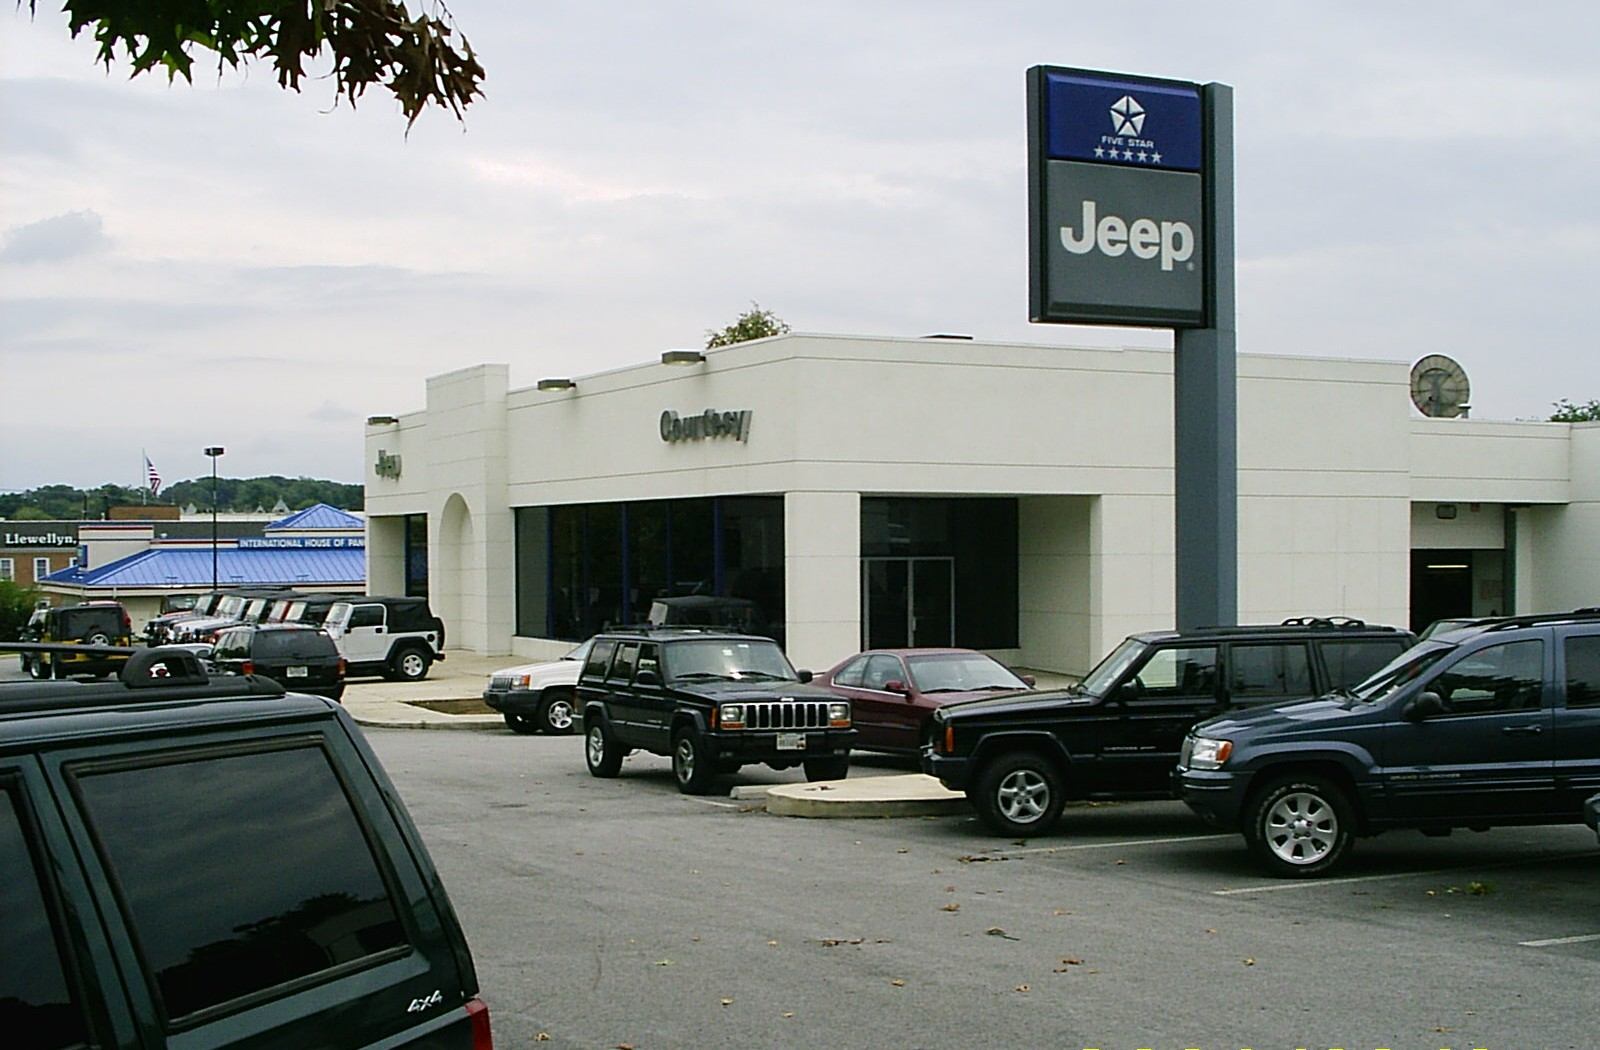
\includegraphics[scale=0.06]{CarDealer1}}
First, let's find out how much the car actually costs you.

The down payment is the amount that is due at the beginning, so if we add that to 60 payments of \$550, we'll have the total amount that comes out of your pocket:
\[\$500 + (60)(\$550) = \$33,500\]

This means that you pay \$33,500 for a \$25,000 car, and the difference is the interest on the loan:\marginnote{\footnotesize\textcolor{black!60}{Photo by Christopher Ziemnowicz}}
\[\$33,500 - \$25,000 = \$8500\]

Are you really willing to pay \$8500 in interest to have the car now, or can you save up first and pay for it in cash---at least in part---to reduce this interest cost?
\end{example}

\begin{try}[http://izzomath.com/103text/finance/example5.3/story.html]
A boat costs \$12,000, and you're offered a loan that requires \$1000 down and \$250 a month for 60 months.  Find the total amount you would pay for the boat and the amount of interest you would pay with this loan.
\end{try}

This example emphasizes an important point: when you're offered a loan, don't focus on the monthly payment; instead, calculate the total cost of the loan and decide if it is worth it to you.
\vfill
\pagebreak

\subsection{Mortgages}
At some point, you'll most likely encounter a \textbf{mortgage}, which is a long-term fixed installment loan, most commonly used to purchase a house.  However, a mortgage is simply a large loan used to purchase property, where the property serves as collateral for the loan.  In case you happen to care, the word ``mortgage'' comes from the Old French \textit{mort} ``dead'' -- \textit{gage} ``pledge.''  The idea of a ``dead pledge'' is that the responsibility dies when the debt is paid off.\\

\marginnote{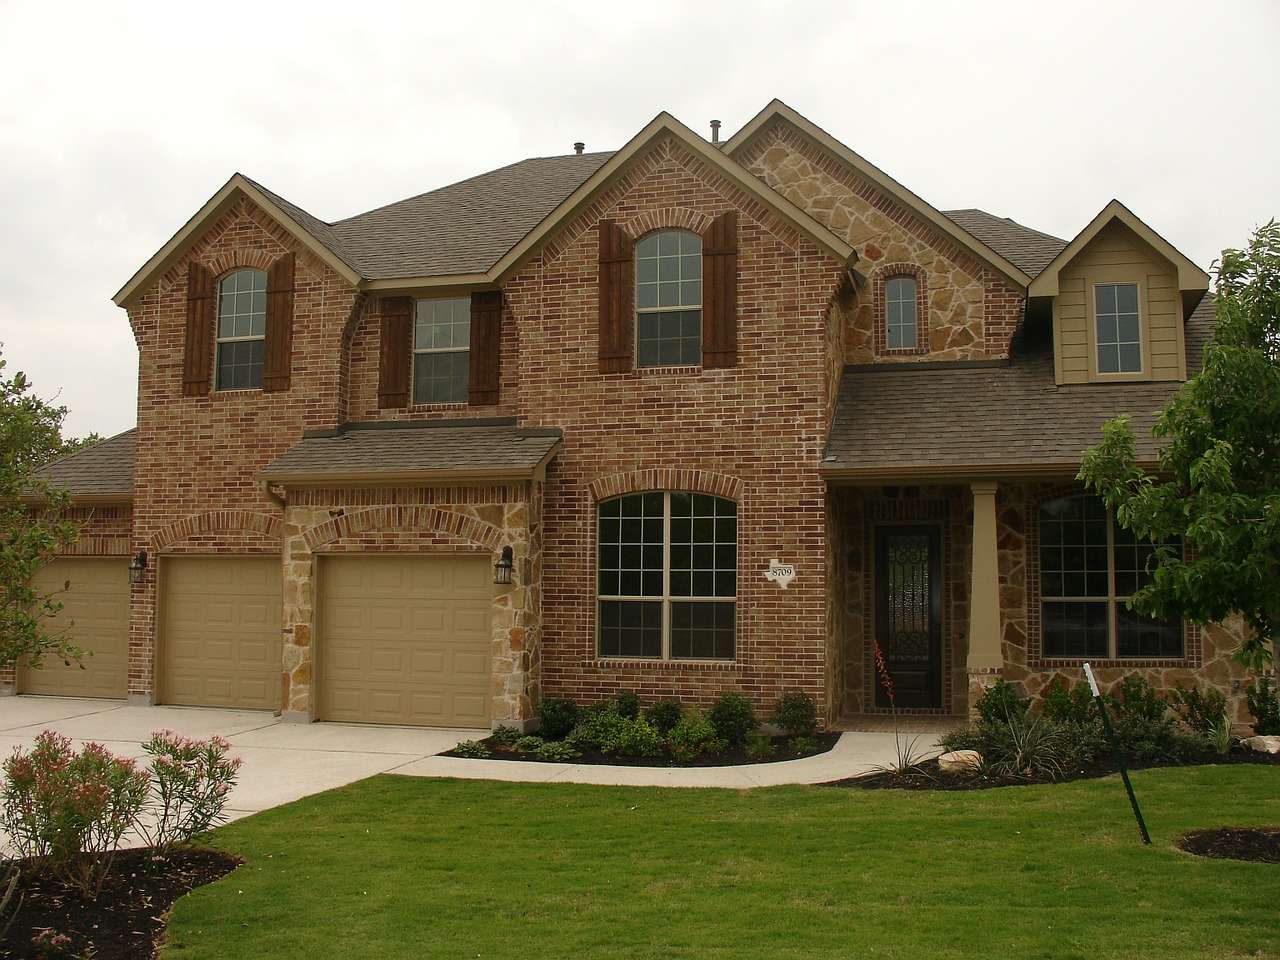
\includegraphics[scale=0.08]{House2}}
We'll focus on mortgages that are used to buy homes in this section, since that is the most practical application.  Most of us don't have the cash to buy a home upfront, so instead we find a bank that is willing to loan us enough to do so.  However, the bank usually isn't willing to loan the entire amount; from their perspective, if a debtor doesn't have anything invested in the loan, they're more likely to \textit{default} on the loan, meaning that they stop making payments and lose the home.  To avoid this, the bank requires a \textbf{down payment}, which means that the buyer is required to come up with a portion of the cost of the home.  The more that the buyer can put down on the home, the less they have to borrow, so they end up paying much less in interest.  Ideally, a buyer is able to put down 20\% of the price of the home; if not, most banks require \textit{mortgage insurance}---which is an extra monthly charge---because clients with less stake in the home are more likely to default, so the bank protects itself with this insurance.

\begin{proc}{Mortgage Terminology}
\begin{itemize}
\item \textbf{Down Payment:} A portion of the cost of the home that the buyer is required to pay before the bank is willing to offer them a loan.
\item \textbf{Loan Amount:} The amount that the bank pays for the home (the cost of the home minus the down payment), which the buyer begins to pay back with monthly payments.
\item \textbf{Closing Costs:} Administrative costs that the bank charges when a mortgage is acquired.  These are usually expressed as \textit{points}, which refers to a percentage of the \textit{loan amount}---not the cost of the home.  Often in negotiations, the seller of the home will agree to cover closing costs in order to make the sale, since the buyer is using all of their available cash to cover the down payment and the seller is the one who will receive a lump sum payment from the bank, so they'll have more cash available.
\end{itemize}
\end{proc}

\begin{example}[https://www.youtube.com/watch?v=lcCuSQxX--Y]{Buying a Condo}
The price of a condominium is \$180,000.  The bank requires a 5\% down payment and one point at closing.  You plan to finance the condominium with a 30-year mortgage at 4\% interest.\\

\begin{center}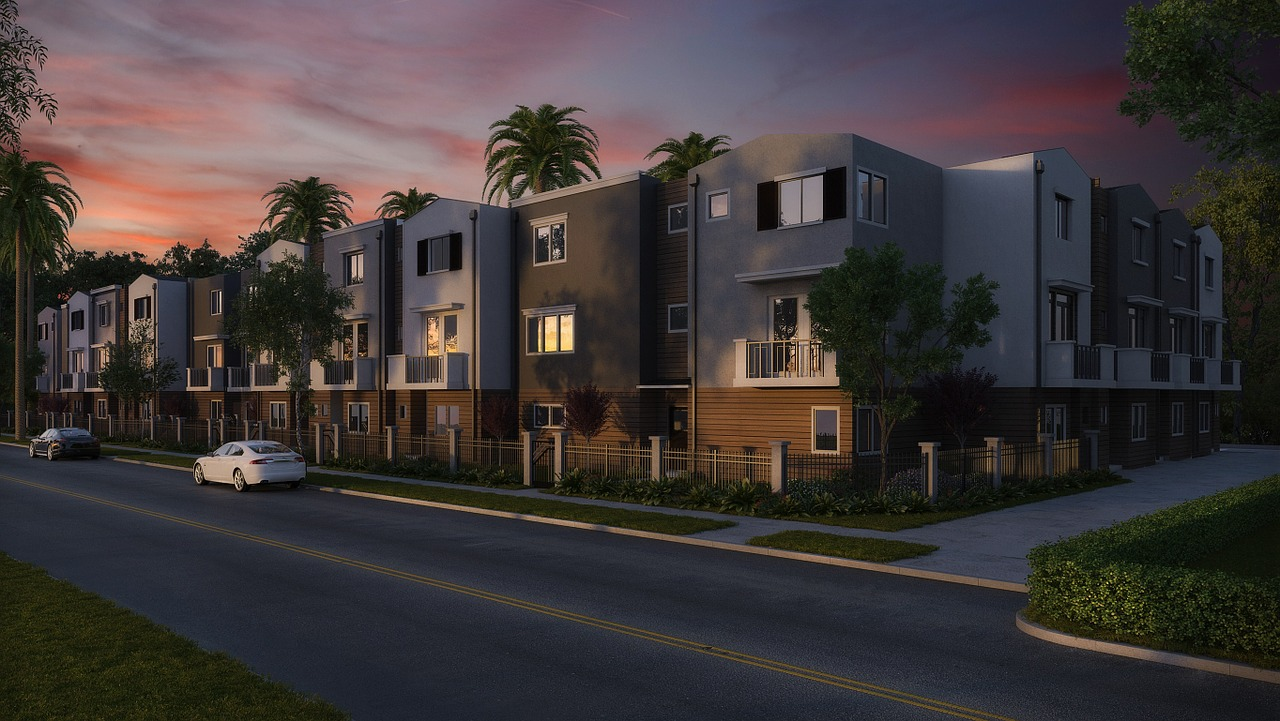
\includegraphics[scale=0.25]{Condo1}\end{center}
\vfill
\pagebreak
\begin{enumerate}[(a)]
\item Find the required down payment.

This is simply 5\% of the sale price, \$180,000:
\[(0.05)(\$180,000) = \$9000\]
Notice that this is the \textit{minimum} down payment; if you were able to put down more than this, that would be a good idea, since it would reduce the interest that you would have to pay in the long run.
\pagebreak

\item Find the loan amount.

This is simply the sale price minus the down payment:
\[\$180,000 - \$9000 = \$171,000\]

\item Find the closing costs.

This will be 1\% of the loan amount, and won't reduce the amount of the loan; it is simply a fee added for the privilege of taking out the loan:
\[(0.01)(\$171,000) = \$1710\]

\item Find the monthly payment.

Here we use the formula for the payment on a fixed installment loan---notice that $n=12$ since this is a monthly payment:
\begin{align*}
PMT &= \dfrac{P\left(\dfrac{r}{n}\right)}{1-\left(1+\dfrac{r}{n}\right)^{-nt}}\\
&= \dfrac{\$171,000\left(\dfrac{0.04}{12}\right)}{1-\left(1+\dfrac{0.04}{12}\right)^{-(12)(30)}}\\
&= \$816.38
\end{align*}

\item Find the total interest paid over 30 years.

Simply find the total amount paid---the down payment plus the 360 monthly payments of \$816.38---and subtract the cost of the condo:
\[\$9000+(360)(\$816.38)-\$180,000 = \$122,896.86\]
Notice that you'll end up paying close to the cost of the condo just in interest.
\end{enumerate}
\end{example}

\begin{try}[http://izzomath.com/103text/finance/example5.4/story.html]
The price of a home is \$340,000.  The bank requires a 10\% down payment and two points at closing.  You plan to finance the condominium with a 30-year mortgage at 3.5\% interest.
\begin{enumerate}[(a)]
\item Find the required down payment.
\item Find the loan amount.
\item Find the closing costs.
\item Find the monthly payment.
\item Find the total interest paid over 30 years.
\end{enumerate}
\end{try}
\pagebreak

\begin{example}[https://www.youtube.com/watch?v=J5Buue07f44]{Comparing Two Mortgages}
The price of a home is \$160,000.  The bank requires a 15\% down payment, and you're offered two mortgage options: 15-year fixed at 5\% or 30-year fixed at 5\% (the term \textit{fixed} here refers to a fixed interest rate, which will be constant throughout the life of the loan, as opposed to an \textit{adjustable-rate mortgage}, or ARM).  Calculate the amount of interest paid for each option and compare the results.\\

\marginnote{\bfseries Solution}
The 15\% down payment will be $(0.15)(\$160,000) = \$24,000$, so the loan amount will be $\$160,000-\$24,000 = \$136,000$.
\begin{enumerate}[(a)]
\item The 15-year mortgage:
\begin{align*}
PMT &= \dfrac{P\left(\dfrac{r}{n}\right)}{1-\left(1+\dfrac{r}{n}\right)^{-nt}}\\
&= \dfrac{\$136,000\left(\dfrac{0.05}{12}\right)}{1-\left(1+\dfrac{0.05}{12}\right)^{-(12)(15)}}\\
&= \$1075.48
\end{align*}

Thus, the amount of interest paid is the monthly payment times 180 (12 payments a year for 15 years) minus the loan amount:
\[(180)(\$1075.48)-\$136,000 = \$57,586.40\]

\item The 30-year mortgage:
\begin{align*}
PMT &= \dfrac{\$136,000\left(\dfrac{0.05}{12}\right)}{1-\left(1+\dfrac{0.05}{12}\right)^{-(12)(30)}}\\
&= \$730.08
\end{align*}

Here there are 360 payments (12 payments a year for 30 years):
\[(360)(\$730.08)-\$136,000 = \$126,828.80\]
\end{enumerate}

If all you see is the monthly payments, the 30-year mortgage is attractive, since the payment is so much lower.  However, over time, you'll pay nearly \$70,000 more in interest simply by stretching the payments over more time.  Now, of course, you may not be able to afford the payments of the 15-year mortgage, so you may be forced to take a longer loan.\\

Because shorter mortgages save so much on interest, banks usually offer lower interest rates on longer mortgages than they do on short ones.
\end{example}
\vfill
\pagebreak

\paragraph{Amortization Schedules}
We've already seen a sort of amortization schedule at the introduction to installment loans with the table that broke down payments one by one.  Here we'll show a more typical layout for an amortization table.

\begin{formula}{Amortization Table}
An \textbf{amortization table} simply lists the payments of an installment loan in order, showing the amount of each payment that goes toward interest that goes to toward principal.  It is simple but tedious to produce (in practice, spreadsheet programs handle the repetitive calculations).

The key feature of amortization tables, though, is this partitioning of the payment into the amount that goes toward interest and the amount that pays down the loan principal (the two amounts will, of course, add up to the total monthly payment).  As noted earlier, early payments will go largely toward interest and final payments will go mostly toward principal.\\

An amortization table will typically have four columns: the payment number, the interest for that payment, the amount of that payment that goes toward principal, and the remaining balance after the payment.

\begin{center}
\begin{tabular}{|c | c | c | c|}
\hline
Payment Number & Interest Payment & Principal Payment & Loan Balance\\
\hline
& & &
\end{tabular}
\end{center}
\end{formula}

Let's illustrate this with an example.

\begin{example}[https://www.youtube.com/watch?v=bgFXXvgNB0g]{Loan Amortization Schedule}
Suppose you take out a 20-year mortgage for \$200,000 at 7\% interest, with monthly payments of \$1550.60 (we know how to calculate this now, but it is given to us to simplify this example).  Prepare an amortization schedule for this loan.\\

\marginnote{\bfseries Solution}
Only one calculation is really needed at each stage---calculating the interest due for that month (everything else follows from that).  To calculate the interest due for a particular month, use the simple interest formula ($I=Prt$); since we're only looking at one payment period, there's no compounding happening.  The principal $P$ will be the loan balance at that point, $r$ is the same for every payment, and $t$ will be 1/12, since we're dealing with a month, a twelfth of a year.
\begin{enumerate}
\item The first payment:
\begin{align*}
\textrm{Interest } &= Prt = (\$200,000)(0.07)\left(\dfrac{1}{12}\right) = \$1166.67\\
\textrm{Principal Payment } &= \textrm{ Monthly Payment } - \textrm{ Interest}\\
&= \$1550.60 - \$1166.67 = \$383.93\\
\textrm{Balance } &= \textrm{ Previous Balance } - \textrm{ Principal Payment}\\
&= \$200,000 = \$383.93 = \$199,616.07
\end{align*}

\item The second payment: the starting balance for the second month is the final balance at the end of the first month, \$199,616.07.
\begin{align*}
\textrm{Interest } &= Prt = (\$199,616.07)(0.07)\left(\dfrac{1}{12}\right) = \$1164.43\\
\textrm{Principal Payment } &=  \$1550.60 - \$1164.43 = \$386.17\\
\textrm{Balance } &= \$200,000 = \$386.17 = \$199,229.90
\end{align*}
\end{enumerate}
To fill out the rest of the table, we could continue these calculations until we've covered all 240 payments, but of course this is far too tedious to do by hand, so we have a computer do it for us.  The table below shows a few of the payments, skipping through to show payments at various stages of the loan.
\begin{center}
\begin{tabular}{|>{\centering\arraybackslash\hspace{0pt}}p{1.1in} | >{\centering\arraybackslash\hspace{0pt}}p{1.1in} | >{\centering\arraybackslash\hspace{0pt}}p{1.2in} | >{\centering\arraybackslash\hspace{0pt}}p{1in}|}
\hline
{\small Payment Number} & {\small Interest Payment} & {\small Principal Payment} & {\small Balance of Loan}\\
\hline
1 & 1166.67 & 383.93 & 199616.07\\
\hline
2 & 1164.43 & 386.17 & 199229.90\\
\hline
3 & 1162.17 & 388.42 & 198841.47\\
\hline
4 & 1159.91 & 390.69 & 198450.79\\
\hline
\vdots & \vdots & \vdots & \vdots\\
\hline
30 & 1096.12 & 454.47 & 187452.64\\
\hline
31 & 1093.47 & 457.12 & 186995.52\\
\hline
\vdots & \vdots & \vdots & \vdots\\
\hline
145 & 663.44 & 887.16 & 112845.43\\
\hline
146 & 658.26 & 892.33 & 111953.09\\
\hline
\vdots & \vdots & \vdots & \vdots\\
\hline
239 & 17.93 & 1532.66 & 1541.61\\
\hline
240 & 8.99 & 1541.61 & 0.00\\
\hline
\end{tabular}
\end{center}

This illustrates the key features of an amortization table:
\begin{itemize}
\item The interest payment and principal payment in each row add up to the same monthly payment.
\item The balance of the loan slowly shrinks and goes exactly to zero with the last payment.
\item The amount of the payment that goes to interest shrinks each month and the amount that goes to paying down the principal grows by an equal amount.
\end{itemize}
\end{example}

\begin{try}[http://izzomath.com/103text/finance/example5.6/story.html]
If you take out a loan for \$175,000 at 4.5\% interest for 30 years, with a monthly payment of \$886.70, find values for A-F that will correctly fill out the first two rows of the amortization table below.
\begin{center}
\begin{tabular}{|>{\centering\arraybackslash\hspace{0pt}}p{1in} | >{\centering\arraybackslash\hspace{0pt}}p{1in} | >{\centering\arraybackslash\hspace{0pt}}p{1in} | >{\centering\arraybackslash\hspace{0pt}}p{1in}|}
\hline
{\small Payment Number} & {\small Interest Payment} & {\small Principal Payment} & {\small Balance of Loan}\\
\hline
1 & A & B & C\\
\hline
2 & D & E & F\\
\hline
& & &
\end{tabular}
\end{center}
\end{try}

\subsection{Credit Cards}
So far, we've dealt with \textit{fixed installment loans}, meaning that a specified amount is loaned and paid back with fixed payments in such a way that the balance goes to zero with the final scheduled payment.

On the other hand, there are \textbf{open-ended installment loans}, which require a variable payment each month, and the loan has no guaranteed end date; payments are made for as long as necessary to pay off the loan.  The most common example is a credit card, where the total balance does not have to be paid off each month, and any unpaid balance rolls over to the following month.  Of course, credit card companies take advantage of the ease of payment to rack up huge interest charges---credit card interest rates are among the highest you'll likely see.  If, on the other hand, you pay off the entire balance each month, treating the card more like a debit card, you'll never pay any interest charges to your credit card company.
\begin{center}
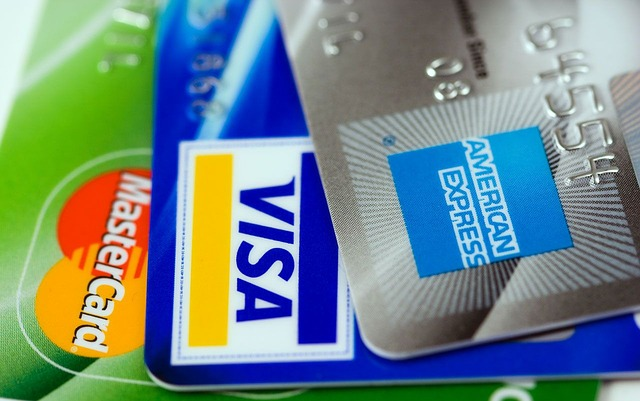
\includegraphics[scale=0.25]{CreditCards1}
\end{center}
\vfill
\pagebreak

\paragraph{Average Daily Balance Method} Different credit card companies calculate interest in different ways, all using the simple interest formula ($I=Prt$).  The difference lies in how $P$ is calculated; since the balance is constantly changing all month, they need a way to combine this all into a single principal.  The method we'll illustrate is called the \textit{average daily balance method}, which as the name suggests, takes the average of the balance on each day of the month.  Thus, if the balance was \$100 on the first 15 days of the month and \$200 on the last 15 days, the average daily balance will be \$150.

To find the average daily balance, add up the balance for each day and divide by the number of days.  In practice, we'll use a table to simplify the calculations by multiplying each different balance by the number of days that the card carried that balance.

\begin{example}[https://www.youtube.com/watch?v=ZUEQu_e2TqY]{Credit Card Charges}
Suppose your VISA card calculates interest using the average daily balance method, and the monthly interest rate is 1.5\% (notice that this means that the nominal annual rate is $1.5\% \times 12 = 18\%$, which is not at all unusually high for a credit card).  The itemized billing for the month of December is shown below.
\begin{center}
\begin{tabular}{l l l}
Detail & Date & Amount\\
\hline
Unpaid balance & December 1 & \$1500\\
Payment received & December 4 & \$300\\
Groceries & December 8 & \$125\\
Gas & December 15 & \$45\\
Wendy's & December 22 & \$8.50\\
Last day of billing period & December 31 &\\
Payment Due Date & January 7 &\\
\end{tabular}
\end{center}

\begin{enumerate}[(a)]
\item Find the average daily balance.

To do this, we'll build a table to keep track of the unpaid balance after each transaction, and how long that unpaid balance lasts.

\begin{center}
\begin{tabular}{l l}
Date & Unpaid Balance\\
\hline
December 1 & \$1500\\
December 4 & \$1200\\
December 8 & \$1325\\
December 15 & \$1370\\
December 22 & \$1378.50\\
\end{tabular}
\end{center}

Now calculate how many days each balance lasted and multiply the balance by the number of days it lasted; this lets us quickly add up the balance for each day so that we can find the average by dividing this by the number of days.
\begin{center}
\begin{tabular}{l l p{0.7in} p{1.5in}}
Date & Unpaid Balance & Number of Days & (Unpaid balance) $\times$ (Number of Days)\\
\hline
December 1 & \$1500 & 3 & \$4500\\
December 4 & \$1200 & 4 & \$4800\\
December 8 & \$1325 & 7 & \$9275\\
December 15 & \$1370 & 7 & \$9590\\
December 22 & \$1378.50 & 10 & \$12,406.50\\
\hline
\textbf{Total:} & & 31 & \$40,571.50
\end{tabular}
\end{center}

The average daily balance is then the sum of the daily balances divided by 31, the number of days in the billing period:
\[\dfrac{\$40,571.50}{31} = \$1308.76\]

\item Find the interest due for December.

Use the simple interest formula, noting that since the interest rate is given as a \textit{monthly} rate, $t=1$ since we're dealing with a single month:
\[I=Prt = (\$1308.76)(0.015)(1) = \$19.63\]

\item Find the total balance owed on the last day of the billing period.

This is the final balance plus the interest charges:
\[\$1378.50 + \$19.63 = \$1398.13\]

\item This credit card requires a \$15 minimum monthly payment or 1/36 of the amount due, whichever is higher.  What is the minimum monthly payment due by January 7?

Since 1.36 of the amount due is $\$1398.13/36 = \$38.84$, which is more than \$15, the minimum payment due will be \$38.84.
\end{enumerate}
\end{example}

\begin{try}[http://izzomath.com/103text/finance/example5.7/story.html]
Suppose your VISA card calculates interest using the average daily balance method, and the monthly interest rate is 1.8\%.  The itemized billing for the month of May is shown below.
\begin{center}
\begin{tabular}{l l l}
Detail & Date & Amount\\
\hline
Unpaid balance & May 1 & \$850\\
Payment received & May 5 & \$200\\
Groceries & May 7 & \$240\\
Gas & May 13 & \$33\\
Jewelry Store & May 25 & \$575\\
Last day of billing period & May 31 &\\
Payment Due Date & June 7 &\\
\end{tabular}
\end{center}

\begin{enumerate}[(a)]
\item Find the average daily balance.
\item Find the interest due for this month.
\item Find the total balance owed on the last day of the billing period.
\item This credit card requires a \$20 minimum payment or 1/24 of the amount due, whichever is higher.  What is the minimum monthly payment due for this month?
\end{enumerate}
\end{try}

We'll finish this discussion by taking another look at the trap of the minimum payment; we'll use the numbers from the preceding example.  A minimum payment of \$38.84 on a balance of \$1398.13 sounds pretty reasonable, but think about how long it would take to pay off this balance by only making the minimum payment each month (even without adding further charges), since the majority of the minimum payment will go toward interest.

Skipping over the details (this can be figured out using a simple spreadsheet), if you started with a balance of \$1398.13 and never added another charge, just making the minimum payment each month, it would take 123 months to pay it off, or over 10 years.  In doing so, you would end up paying a total of \$2571.46, or nearly twice what you owed.  The lesson is simple: pay off your credit card in full as much as possible, and don't live beyond your means in a way that requires the use of credit to get by.

\begin{exercises}
\ptwo{If you take out an auto loan of \$8500 at 5\% interest for 48 months, what will your monthly payment be?}
\ptwo{If you borrow \$13,000 to buy a boat, and the bank charges 7\% interest for 72 months, how much will you have to pay each month?}

\ptwo{Janine bought \$3000 of new furniture on credit.  Because her credit score isn't very good, the store is charging her a fairly high interest rate on the loan: 16\%.  If she agreed to pay off the furniture over two years, how much will she have to pay each month?}
\ptwo{Carly financed a new \$1200 television at 12\% for 48 months.  How much will she have to pay every month to pay this off?}

\ptwo{If you want to buy a car, and you can afford a monthly payment of \$175, how large of a loan can you get at 4.8\% interest over 60 months?}
\ptwo{Mary is going to finance new office equipment at a 2\% rate over a 4 year term.  If she can afford monthly payments of \$100, how much can she pay for the new office equipment?}

\ptwo{If you buy a \$33,000 car for \$1000 down and monthly payments of \$685 for 60 months, how much will you pay in total for the car?}
\ptwo{A car costs \$27,000, and you're offered a loan that requires \$800 down and a monthly payment of \$575 for 60 months, how much will you pay in interest?}

\ptwo{You want to buy a \$200,000 home.  You plan to pay 10\% as a down payment, and take out a 30-year loan at 4.75\% for the rest.  The bank requires 2 points at closing.
\begin{enumerate}[(a)]
\item How much is the loan amount going to be?
\item How much are the closing costs?
\item What will your monthly payments be?
\item How much will you pay in interest over the life of the loan?
\end{enumerate}}
\ptwo{You want to buy a \$375,000 home.  You plan to pay 20\% as a down payment, and take out a 30-year loan at 3.9\% for the rest.  The bank requires 1 point at closing.
\begin{enumerate}[(a)]
\item How much is the loan amount going to be?
\item How much are the closing costs?
\item What will your monthly payments be?
\item How much will you pay in interest over the life of the loan?
\end{enumerate}}

\ptwo{You can afford a \$900 per month mortgage payment.  You've found a 30-year loan at 5\% interest.
\begin{enumerate}[(a)]
\item How big of a loan can you afford?
\item How much total money will you pay the bank?
\item How much of that money is interest?
\end{enumerate}}
\ptwo{You can afford a \$17,900 per month mortgage payment.  You've found a 15-year loan at 3.85\% interest.
\begin{enumerate}[(a)]
\item How big of a loan can you afford?
\item How much total money will you pay the bank?
\item How much of that money is interest?
\end{enumerate}}

\pone{Suppose you take out a \$315,000 mortgage for 30 years at 4.5\% interest.
\begin{enumerate}[(a)]
\item Find the monthly payment on this mortgage.
\item Fill out the first two rows of the amortization schedule below.
\begin{center}
\begin{tabular}{|>{\centering\arraybackslash\hspace{0pt}}p{1.1in} | >{\centering\arraybackslash\hspace{0pt}}p{1.1in} | >{\centering\arraybackslash\hspace{0pt}}p{1.2in} | >{\centering\arraybackslash\hspace{0pt}}p{1in}|}
\hline
{\small Payment Number} & {\small Interest Payment} & {\small Principal Payment} & {\small Balance of Loan}\\
\hline
1 & & & \\
\hline
2 & & & \\
\hline
& & &
\end{tabular}
\end{center}
\end{enumerate}}

\pone{Suppose you take out a \$180,000 mortgage for 15 years at 3.7\% interest.
\begin{enumerate}[(a)]
\item Find the monthly payment on this mortgage.
\item Fill out the first two rows of the amortization schedule below.
\begin{center}
\begin{tabular}{|>{\centering\arraybackslash\hspace{0pt}}p{1.1in} | >{\centering\arraybackslash\hspace{0pt}}p{1.1in} | >{\centering\arraybackslash\hspace{0pt}}p{1.2in} | >{\centering\arraybackslash\hspace{0pt}}p{1in}|}
\hline
{\small Payment Number} & {\small Interest Payment} & {\small Principal Payment} & {\small Balance of Loan}\\
\hline
1 & & & \\
\hline
2 & & & \\
\hline
& & &
\end{tabular}
\end{center}
\end{enumerate}}

\ptwo{Suppose your VISA card calculates interest using the average daily balance method, and the monthly interest rate is 1.4\%.  The itemized billing for the month of April is shown below.\\

\begin{tabular}{l l l}
Detail & Date & Amount\\
\hline
Unpaid balance & April 1 & \$1100\\
Payment received & April 3 & \$500\\
New computer & April 11 & \$750\\
Books & April 15 & \$65\\
Mattress & April 28 & \$600\\
Last day of billing period & April 30 &\\
Payment Due Date & May 7 &\\
\end{tabular}

\begin{enumerate}[(a)]
\item Find the average daily balance.
\item Find the interest due for this month.
\item Find the total balance owed on the last day of the billing period.
\item This credit card requires a \$20 minimum payment or 1/36 of the amount due, whichever is higher.  What is the minimum monthly payment due for this month?
\end{enumerate}}
\ptwo{Suppose your MasterCard calculates interest using the average daily balance method, and the monthly interest rate is 2.1\%.  The itemized billing for the month of August is shown below.\\

\begin{tabular}{l l l}
Detail & Date & Amount\\
\hline
Unpaid balance & August 1 & \$300\\
Payment received & August 9 & \$100\\
Tuition & August 10 & \$4500\\
Textbooks & August 18 & \$350\\
Groceries & August 25 & \$180\\
Last day of billing period & August 31 &\\
Payment Due Date & September 7 &\\
\end{tabular}

\begin{enumerate}[(a)]
\item Find the average daily balance.
\item Find the interest due for this month.
\item Find the total balance owed on the last day of the billing period.
\item This credit card requires a \$15 minimum payment or 1/24 of the amount due, whichever is higher.  What is the minimum monthly payment due for this month?
\end{enumerate}}
\vfill
\pagebreak

\pone{\textbf{Project: Finding a Mortgage}

You and your family are looking to move and are shopping for a house.  Your job is to find a mortgage that you can afford.

You may choose your family size---you can be married with kids, married without kids, or single.  You may also pick anywhere in the country that you'd like to live, but you can only make the median income listed for the state you choose.  If you are married, you can assume that both you and your spouse are working and each are paid the median income for that state.

\begin{enumerate}
\item Decide where you want to live.  Do some research and find the median income for that state, and decide whether you are single or married, and whether or not you have children.
\item Search \href{http://www.realtor.com}{realtor.com} or a similar website to find a house that fits your family's needs.  Take note of the
\begin{itemize}
\item List price of the home.
\item Property taxes listed under the ``Property History'' tab.  If property taxes are not listed, estimate the annual property taxes as 2\% of the purchase price.
\end{itemize}
\item Estimate the down payment you can afford, and take note of the principal of the loan that you will need.
\item There are several options for financing your new home.  These include obtaining a fixed 15-year mortgage, a fixed 30-year mortgage or an adjustable rate mortgage.  Go to \href{http://www.ratesandpoints.com}{www.ratesandpoints.com} $\longrightarrow$ ``Mortgage Analyst.''  First click on ``Go'' for a 30 FRM (30-year fixed rate mortgage).  Pick two options---one with points and one without.  Repeat this process for 15 FRM.  Record these results in the table below.
\begin{center}
\begin{tabular}{|p{0.75in} | p{1.5in} | p{2in} | p{1.5in}|}
\hline
\textbf{Length of Mortgage} & \textbf{Interest Rate} & \textbf{Monthly Payment (PMT)} & \textbf{Total Cost of Mortgage = Total PMTs + Down Payment + Closing Cost}\\
\hline
& With 0 points & & \\
& Rate $= \line(1,0){30}$ & & \\
15 years & & & \\
& With $\line(1,0){30}$ points & & \\
& Rate $= \line(1,0){30}$ & & \\
\hline
& With 0 points & & \\
& Rate $= \line(1,0){30}$ & & \\
30 years & & & \\
& With $\line(1,0){30}$ points & & \\
& Rate $= \line(1,0){30}$ & & \\
\hline
\end{tabular}
\end{center}
Which option seems like the best?
\end{enumerate}}

\begin{minipage}{0.9\textwidth}
\begin{enumerate}
\setcounter{enumi}{4}
\item Complete the following steps to find if you can afford this home.
\begin{center}
\begin{tabular}{p{3.75in} p{3in}}
\textbf{Monthly Gross Income} &\\
\hspace{0.5in} Borrower's annual income & $\$ \line(1,0){150}$\\
& \\
\hspace{0.5in} Co-borrower's annual income & $+ \line(1,0){150}$\\
& \\
\hspace{0.5in} Total gross annual income & $\$ \line(1,0){150}$\\
\hspace{0.75in} Divide total gross income by 12 & \hspace{0.25in} $\div$ 12\\
& \\
\hspace{0.5in} Total monthly gross income & $\$ \line (1,0){150}$\\
\hspace{0.75in} Find 28\% of this & \hspace{0.25in} $\times 0.28$\\
& \\
\hspace{0.5in} \textbf{Allowable monthly housing cost} & $\$\line(1,0){150}$ (A)\\
& \\
\textbf{Monthly Taxes} &\\
\hspace{0.5in} Home purchase price & $\$ \line(1,0){150}$\\
& \\
\hspace{0.5in} Estimated taxes & $\$ \line(1,0){150}$\\
\hspace{0.75in} Divide taxes by 12 & \hspace{0.25in} $\div 12$\\
& \\
\hspace{0.5in} Monthly taxes & $\$ \line(1,0){150}$ (B)\\
& \\
\textbf{Monthly Housing Cost} & \\
\hspace{0.5in} Monthly mortgage payment & $\$ \line(1,0){150} \ +$\\
& \\
\hspace{0.5in} Estimated monthly taxes (B) & $\$ \line(1,0){150} \ +$\\
& \\
\hspace{0.5in} Condo or homeowner's fee (if applicable) & $\$ \line(1,0){150}$\\
& \\
\textbf{Total Monthly Housing Cost} & $= \$ \line(1,0){140}$ (C)
\end{tabular}
\end{center}
Compare (A) and (C).  Can you afford the house you want to buy?  If not, choose a less expensive house and redo this project.
\end{enumerate}
\end{minipage}

\end{exercises}

\begin{comment}
\chapter{Growth Models}
\begin{center}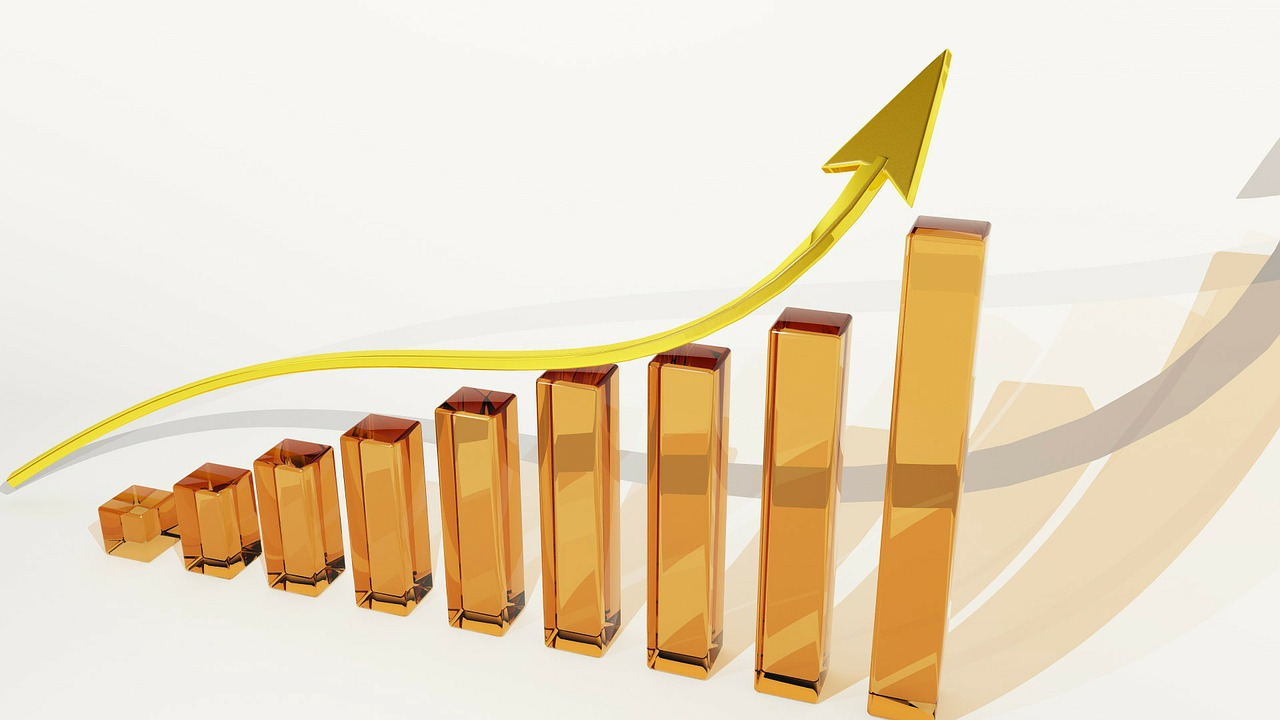
\includegraphics[width=\textwidth, height=4in]{Growth1}\end{center}
From population growth to economic growth, from the study of vibrations to heat transfer, mathematical models of growth and decay provide an important application, giving insight and predicting what the future will hold.

Of course, it is crucial to understand that no mathematical model is perfect.  There will always be a trade-off between the accuracy of a model and its simplicity.  The simpler a model, the more easily we can make predictions with it, but there will be more error in the approximation.  On the other hand, more precise models may be more difficult---or even impossible---to solve.  You should always remember, though, that every model is at best an imperfect representation of the real world, and there will always be some inherent error between what the model predicts and what actually occurs.

The world is too complex to describe in every detail, so every model has simplifying assumptions, and these assumptions need to be spelled out.  A good model uses reasonable assumptions to provide the right balance of simplicity and accuracy.
\vfill
\pagebreak

\section{Linear Models}
\setcounter{ExampleCounter}{1}
\marginnote{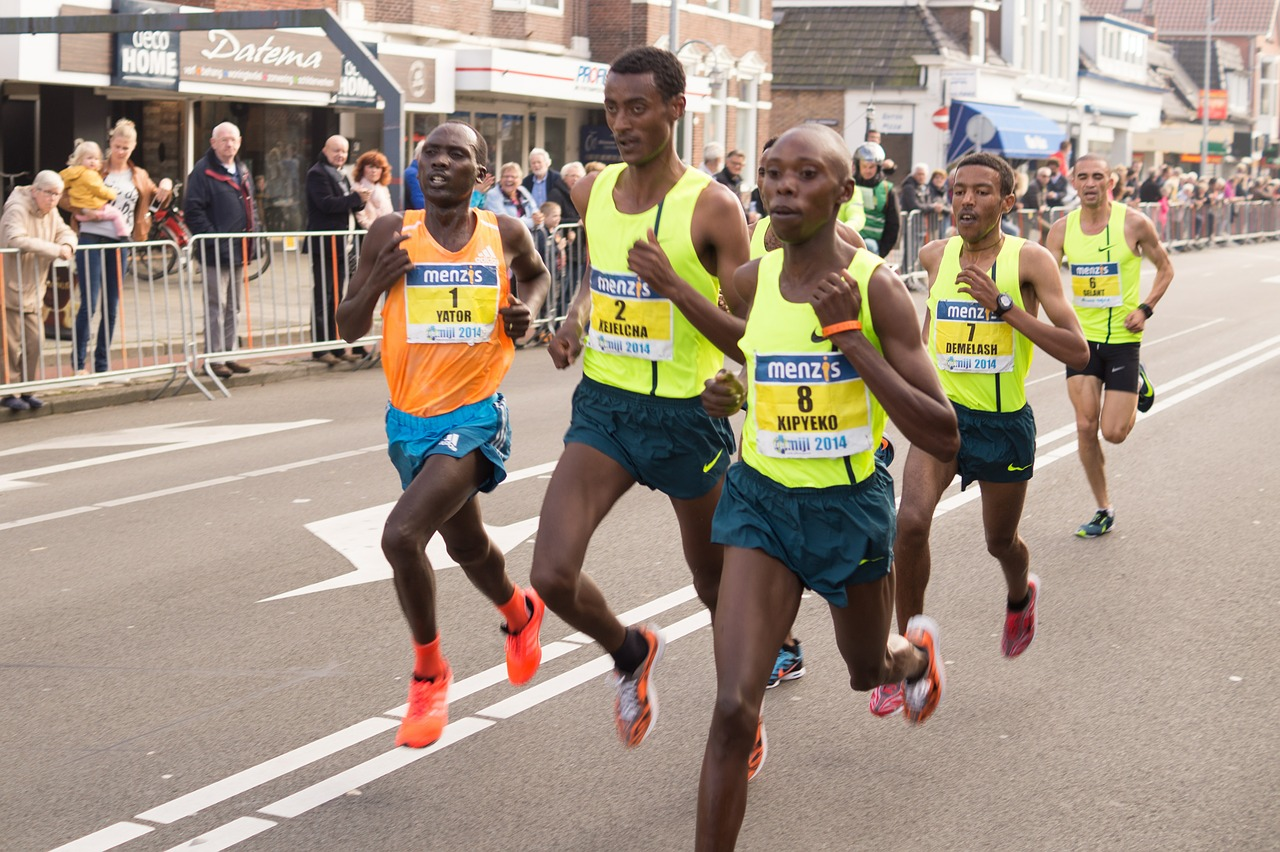
\includegraphics[scale=0.07]{Marathon1}}
If you were training for a marathon and you currently run 3 miles a day, you may choose to increase your distance by half a mile every week.  Can we predict how far you'll be running in six weeks, or how long it will take to reach your goal?  With small numbers like these, you could answer those questions without using an equation, but we'll use this as an example to show how to build a simple model from a scenario like this.

Let $P_t$ represent the number of miles that you run after $t$ weeks, so $P_0$ would be the number of miles you currently run, $P_1$ would represent the number of miles you run after 1 week, and so on.  We can define a \textbf{recursive relationship} like the following one to represent the scenario that was laid out.
\begin{align*}
P_0 &= 3\\
P_t &= P_{t-1} + 0.5
\end{align*}
A recursive relationship is one that relates the next value in a sequence to previous values.  We could use this relationship to go from $P_0$ to $P_1$ to $P_2$ and so on, all the way to $P_6$ to answer the first question, and we could keep going from one value to the next until we reached 26 to answer the second question.  However, this would be tedious and mindless, so instead we prefer an \textbf{explicit equation}, or closed-form equation.  Especially for predictions far into the future, the recursive form is impractical, even though it arises easily from the problem description.

In this case, the explicit form is pretty straightforward, but deriving it from the recursive form will be instructive:
\begin{align*}
P_0 &= 3\\
P_1 &= 3+0.5\\
P_2 &= 3+0.5+0.5 = 3+(0.5)2\\
P_3 &= 3+0.5+0.5+0.5 = 3 + (0.5)3\\
&\vdots\\
P_t &= 3 + 0.5t
\end{align*}

This explicit equation gives an easy way to quickly answer both questions.  We can substitute 6 for $t$ to find that $P_6 = 3+0.5(6) = 6$ miles, and we can substitute 26 for $P_t$ and solve for $t$ to find how long it'll take to reach your goal:
\begin{align*}
26 &= 3+0.5t\\
23 &= 0.5t\\
46 &= t
\end{align*}
It'll take 46 weeks to reach your goal.
\begin{center}
\begin{tikzpicture}
\begin{axis}[
    xmin=0, xmax=47,
    ymin=0, ymax=30,
    axis lines=center,
    axis on top=false,
    domain=0:1,
    x=0.15cm,
    y=0.15cm,
    xtick={5,10,...,45},
    xticklabels={5,10,...,45},
    ytick={0,5,...,25},
    yticklabels={0,5,10,15,20,25,30},
    axis lines=middle,
    axis line style={->},
    x label style={at={(axis description cs:0.5,-0.1)},anchor=north},
    y label style={at={(axis description cs:-0.1,.5)},rotate=90,anchor=south},
    xlabel={Week},
    ylabel={Number of Miles},
    grid=major
    ]
	\addplot [blue,only marks,mark size=1] table {
	0 3
	1 3.5
	2 4
	3 4.5
	4 5
	5 5.5
	6 6
	7 6.5
	8 7
	9 7.5
	10 8
	11 8.5 
	12 9
	13 9.5
	14 10
	15 10.5
	16 11
	17 11.5
	18 12
	19 12.5
	20 13
	21 13.5
	22 14
	23 14.5
	24 15
	25 15.5
	26 16
	27 16.5
	28 17
	29 17.5
	30 18
	31 18.5
	32 19
	33 19.5
	34 20
	35 20.5
	36 21
	37 21.5
	38 22
	39 22.5
	40 23
	41 23.5
	42 24
	43 24.5
	44 25
	45 25.5
	46 26
	};
	%\addplot [blue, thick] table {
	
	%};
\end{axis}
\end{tikzpicture}
\end{center}
%\begin{center}
%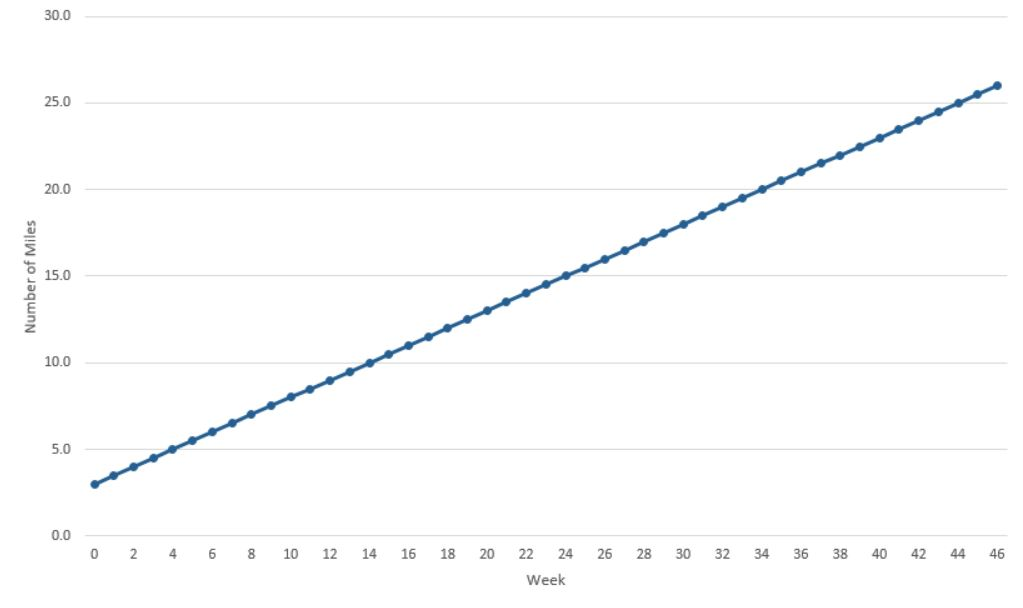
\includegraphics[width=0.8\textwidth]{LinearGraph1}
%\end{center}
This graph shows why we call this \textit{linear} growth.  If we graph the number of miles versus the week, the points lie along a straight line.

This is consistent for every problem where a number grows by a constant amount every time period.

\begin{formula}{Linear Growth}
If some quantity starts at size $P_0$ and grows by $d$ every time period, then the quantity after $t$ time periods can be determined using either of the following relations.\\

Recursive form:
\[P_t = P_{t-1}+d\]

Explicit form:
{\Large \[P_t = P_0 + dt\marginnote{This is the one we'll use in the rest of the examples in this section.}\]}

Here $d$ represents the common difference---the amount that the quantity changes each time $t$ increases by 1.

Notice that this could refer to linear growth or linear decay; if $d$ is negative, the quantity will decrease linearly.
\end{formula}

Knowing that the key to linear growth is this common difference between terms, we can recognize linear growth from data if each term is the previous term plus a constant.
\begin{center}
\begin{tabular}{p{0.5in} p{0.75in} p{1.25in}}
\textbf{Term} & \textbf{Quantity} & \textbf{Difference from Previous Term}\\
\hline
& & \\
0 & 15 & \\
1 & 27 & 12\\
2 & 39 & 12\\
3 & 51 & 12\\
4 & 63 & 12\\
5 & 75 & 12\\
\end{tabular}
\end{center}
As we can observe in this table, if we note that the quantity adds a constant amount each time, we know that the growth is linear, and we can write the closed-form equation given above.\\

Notice that this is exactly the standard linear equation that you've seen in your algebra classes:
\begin{align*}
y &= mx+b\\
P_t &= dt + P_0
\end{align*}
Here, $P_0$ is the $y$-intercept, since it is the starting point, and thus the value when $t=0$.  Also, $d$ is the slope here, or the amount by which the quantity changes when $t$ increases by 1.

These two equations are the same, but as you'll see when modeling, we often rename the pieces to more closely match the names of the real-world quantities we're measuring.

\begin{example}[https://www.youtube.com/watch?v=cpaNK4jbMkA]{Elk Population}
The population of elk in a national forest was measured to be 12,000 in 2011 and 15,000 in 2015.  If the population continues to grow linearly at this rate, what do we expect the elk population to be in 2022?\\

\marginnote{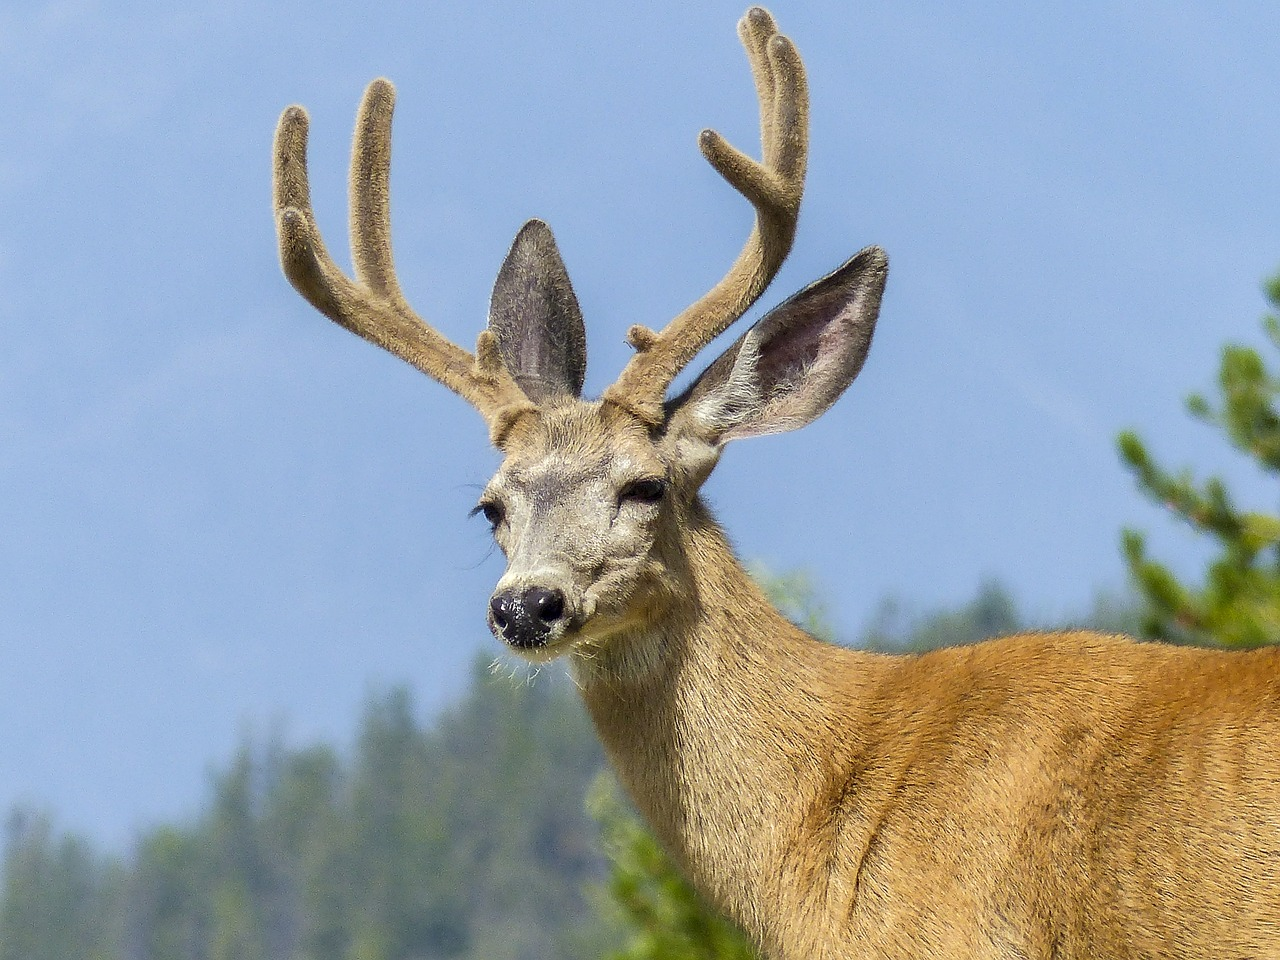
\includegraphics[scale=0.07]{Elk1}}
We first need to define the parts of our linear growth equation.  The initial amount $P_0$ is the amount when $t=0$, but we won't use the actual year 0 as our starting point.  Instead, the initial amount in this problem is given in 2011, so we'll define $t=0$ to be the year 2011, so $P_0=12,000$.\\

Next we need to find $d$, the growth per time period.  Since the time period in this example is one year, we'll need to find how much the population grew each year.
\begin{center}
\begin{tabular}{c c}
\textbf{Year} & \textbf{Population}\\
\hline
0 & 12,000\\
4 & 15,000
\end{tabular}
\end{center}
Since the population grew by 3,000 in 4 years, this represents a growth of 3,000/4 = 750 per year.  Thus $d=750$.\\

Note that this is equivalent to using the slope formula: $\dfrac{\textrm{rise}}{\textrm{run}}$
\[d = \textrm{ slope } = \dfrac{\textrm{change in population}}{\textrm{change in time}} = \dfrac{15,000 - 12,000}{2015 - 2011} = \dfrac{3000}{4} = 750\]

Now we can write the explicit equation that models this population growth:
\[P_t = 12,000 + 750t\]

To answer the question, we note that 2022 corresponds to $t=11$, since 2022 is 11 years after 2011.
\[P_{11} = 12,000 + 750(11) = 20,250 \textrm{ elk}\]
\end{example}

\begin{try}[http://www.izzomath.com/103text/growthmodels/example1.1/story.html]
If we estimated the population of trout in a pond to be 2200 in 2008 and 3500 in 2012, construct a linear model to predict the population in 2017.
\end{try}
\vspace{0.5in}

Now let's try an example with data that is nearly linear, but not exactly.
\begin{example}[https://www.youtube.com/watch?v=QoOdfeLBN0o]{Gasoline Consumption}
Gasoline consumption in the US has been increasing steadily.  Data from 1995 to 2004 is shown below.  Find a linear model for this data, and use it to predict consumption in 2018.  If the trend continues, when will consumption reach 200 billion gallons?\\

\marginnote{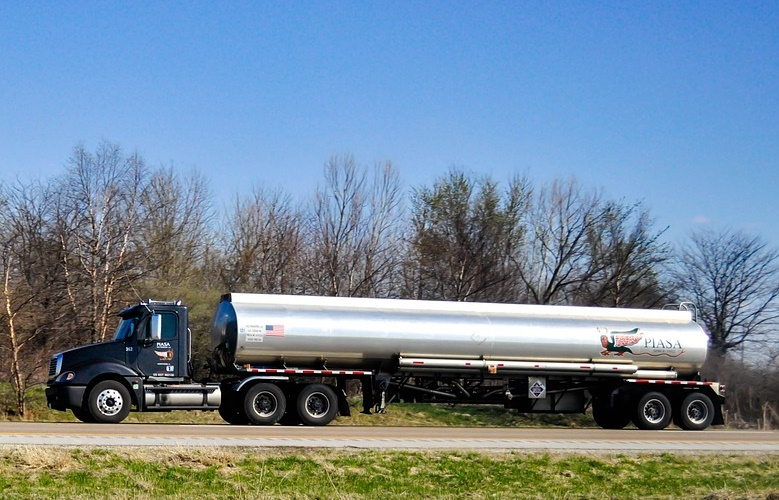
\includegraphics[scale=0.16]{GasTanker1}}
\begin{center}
\begin{tabular}{|p{1in} | c | c | c | c | c | c | c | c | c | c|}
\hline
\textbf{Year} & '95 & '96 & '97 & '98 & '99 & '00 & '01 & '02 & '03 & '04\\
\hline
\textbf{Consumption (billions of gallons)} & 116 & 118 & 119 & 123 & 125 & 126 & 128 & 131 & 133 & 136\\
\hline
\end{tabular}
\end{center}

If we plot this data, it appears to have an approximately linear relationship.
\begin{center}
\begin{tikzpicture}
\begin{axis}[
    xmin=0, xmax=12,
    ymin=0, ymax=25,
    axis lines=center,
    axis on top=false,
    domain=0:1,
    x=0.75cm,
    y=0.15cm,
    xtick={0,1,...,12},
    xticklabels={1994,1995,1996,1997,1998,1999,2000,2001,2002,2003,2004,2005},
    ytick={0,5,...,25},
    yticklabels={115,120,125,130,135,140},
    axis lines=middle,
    axis line style={->},
    x label style={at={(axis description cs:0.5,-0.1)},anchor=north},
    y label style={at={(axis description cs:-0.1,.5)},rotate=90,anchor=south},
    xlabel={Year},
    ylabel={Gas Consumption},
    grid=major
    ]
	\addplot [blue,only marks] table {
	1 1
	2 3
	3 4
	4 8
	5 10
	6 11
	7 13
	8 16
	9 18
	10 21
	};
	%\addplot [blue, thick] table {
	
	%};
\end{axis}
\end{tikzpicture}
\end{center}
%\begin{center}
%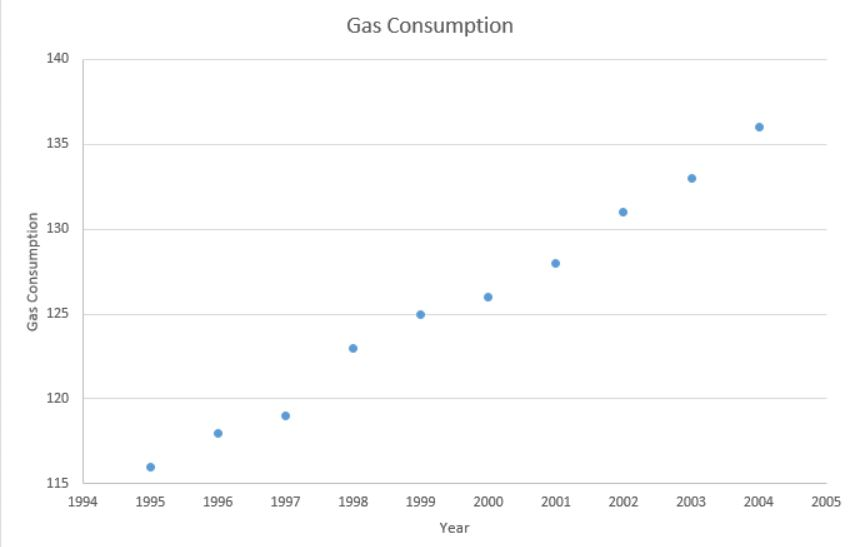
\includegraphics[width=0.8\textwidth]{LinearGraph2}
%\end{center}

While we could use a statistical technique known as \textit{linear regression} to find an equation to model the data, we can find a simple model by using just two pieces of data to calculate an average change.  We'll use the data from 1995 and 2004 for this.\marginnote{We could use the data from any two years to calculate the slope (and we would get slightly different answers), but a common convention is to use the first and last years.  You should follow this convention when answering the homework questions.}
\begin{center}
\begin{tabular}{c | c}
\textbf{Year} & \textbf{Consumption}\\
\hline
1995 & 116\\
2004 & 136
\end{tabular}
\end{center}

\begin{align*}
d &= \textrm{ slope } = \dfrac{\textrm{change in consumption}}{\textrm{change in time}} = \dfrac{136 - 116}{2004 - 1995} = \dfrac{20}{9}\\
&= 2.22 \textrm{ billion gallons per year}
\end{align*}
\vfill
\pagebreak

Now we can write our model:
\[P_t = 116 + 2.2t\]
\begin{center}
\begin{tikzpicture}
\begin{axis}[
    xmin=0, xmax=12,
    ymin=0, ymax=25,
    axis lines=center,
    axis on top=false,
    domain=0:1,
    x=0.75cm,
    y=0.15cm,
    xtick={0,1,...,12},
    xticklabels={1994,1995,1996,1997,1998,1999,2000,2001,2002,2003,2004,2005},
    ytick={0,5,...,25},
    yticklabels={115,120,125,130,135,140},
    axis lines=middle,
    axis line style={->},
    x label style={at={(axis description cs:0.5,-0.1)},anchor=north},
    y label style={at={(axis description cs:-0.1,.5)},rotate=90,anchor=south},
    xlabel={Year},
    ylabel={Gas Consumption},
    grid=major
    ]
	\addplot [blue,only marks] table {
	1 1
	2 3
	3 4
	4 8
	5 10
	6 11
	7 13
	8 16
	9 18
	10 21
	};
	\addplot [blue, thick,dashed,domain=1:10] {2.2*x-1};
\end{axis}
\end{tikzpicture}
\end{center}
%\begin{center}
%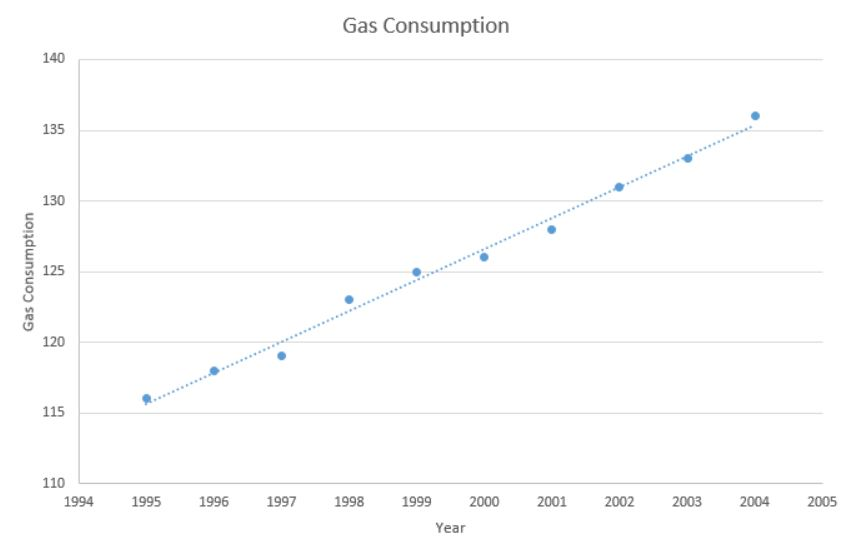
\includegraphics[width=0.8\textwidth]{LinearGraph3}
%\end{center}

Now we can use our model to make predictions about the future, using the simplifying assumption that the previous trend continues unchanged.
\begin{itemize}
\item Predicting gas consumption in 2018, when $t=23$:\marginnote{This example illustrates the two main types of questions that we often want to answer:\\ \text{}\\
1. Predicting the value of what we are measuring at a given point in time.\\ \text{}\\
2. Predicting the point in time when the thing we are measuring will reach a certain value.}
\[P_{23} = 116 + 2.2(23) = 166.6\]
Our model predicts that the US will consume 166.6 billion gallons of gasoline in 2018 if the current trend continues.

\item Predicting when consumption reaches 200 billion gallons:
\begin{align*}
200 &= 116 + 2.2t\\
84 &= 2.2t\\
38.18 &= t
\end{align*}
This model predicts that gas consumption will reach 200 billion gallons about 38 years after 1995, or the year 2033.
\end{itemize}
\end{example}

\begin{try}[http://www.izzomath.com/103text/growthmodels/example1.1/story.html]
The number of stay-at-home fathers in Canada has been growing steadily at an approximately linear rate.  Use the data from the table below to find an explicit formula for the number of stay-at-home fathers and use it to predict the number in 2020.  Use 1976 and 2010 to find the average rate of change.
\begin{center}
\begin{tabular}{|p{1.25in} | c | c | c | c | c|}
\hline
\textbf{Year} & 1976 & 1984 & 1991 & 2000 & 2010\\
\hline
\textbf{Number of stay-at-home fathers} & 20,610 & 28,725 & 43,530 & 47,665 & 53,555\\
\hline
\end{tabular}
\end{center}
\end{try}

Again, we understand that this model is not perfect; the US will most likely not consume exactly 166.6 billion gallons of gas in 2018, but we expect consumption to be \textit{about} that.  In practice, we'll often make predictions and then compare them to actual measured results to assess the accuracy of our model.  A very simple linear model like this will likely have fairly large error; more sophisticated models tend to have smaller errors.

\begin{example}[https://www.youtube.com/watch?v=3GG3aOIc9Pk]{Gym Membership Cost}
The cost, in dollars, of a gym membership for $t$ months can be described by the explicit equation
\[P_t = 70 + 30t.\]
What does this equation tell us?\\

\marginnote{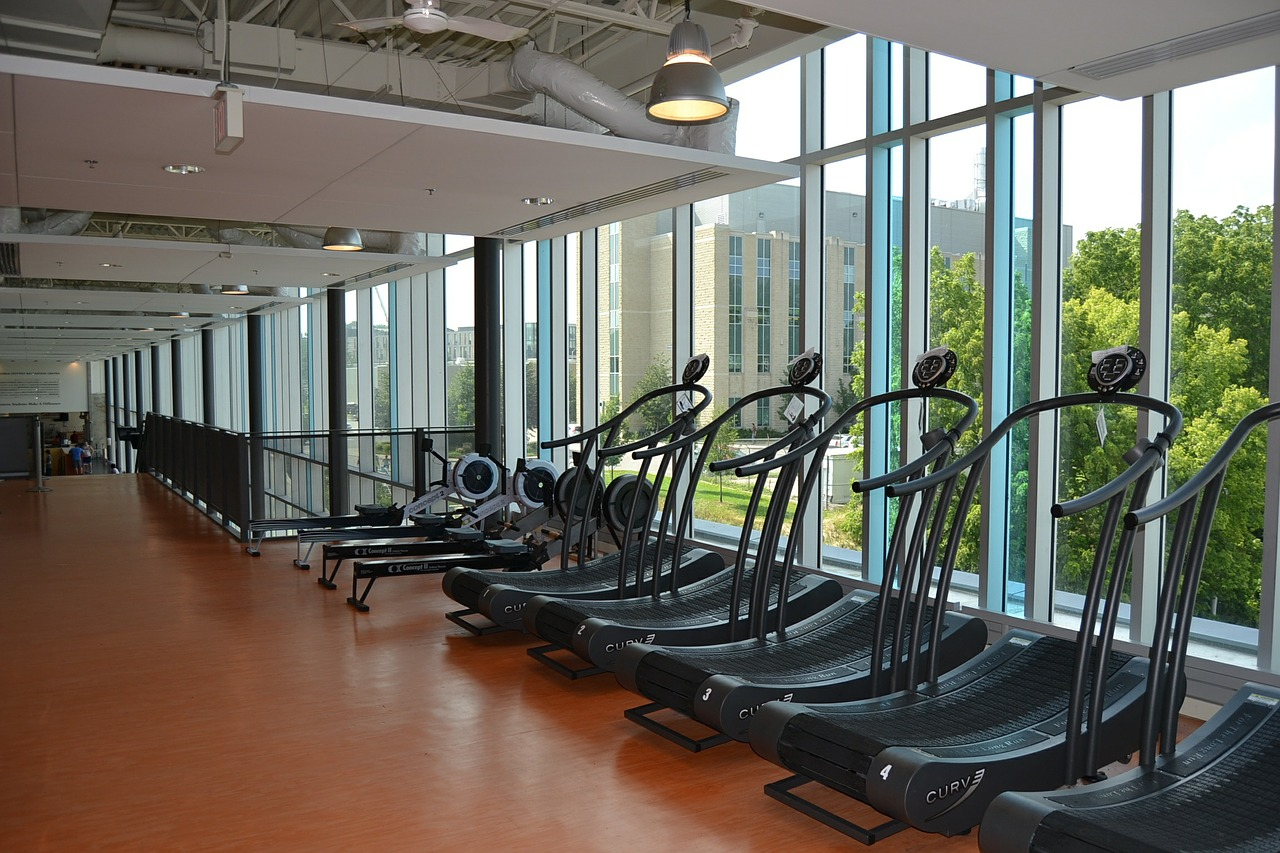
\includegraphics[scale=0.07]{Gym1}}
The value for $P_0$ in this equation is 70, so the initial cost is \$70, which means that there must be a sign-up fee of \$70 to join the gym.\\

The value for $d$ in the equation is 30, so the cost increases by \$30 each month, which means that the monthly membership fee for the gym is \$30 a month.
\end{example}

\subsection{When Good Models Go Bad}
When predicting the future with mathematical models, it is crucial to keep in mind that few trends continue indefinitely.

\begin{example}[https://www.youtube.com/watch?v=7_wAlvsCyDc]{A Boy's Height}
Suppose a four year old boy is currently 39 inches tall, and you are told to expect him to grow 2.5 inches a year.\\

We can set up a growth model, with $t=0$ corresponding to 4 years old.
\[P_t = 39 + 2.5t\]

At six years old (when $t=2$), we would expect him to be
\[P_2 = 44 \textrm{ inches tall},\]
but this model eventually breaks down.  Certainly, we shouldn't expect him to grow at the same rate all his life.  If he did, at age 50 he would be
\[P_{46} = 154 \textrm{ inches } = 12.8 \textrm{ feet tall}.\]
\end{example}

Of course, this boy will not grow at a constant rate, but rather experience growth spurts and ultimately stop growing in his early 20s.  But this example also illustrates that we should check our model against common sense.
\vspace{0.5in}

Let's look at another example that illustrates the need for a common sense check.

\begin{example}[https://www.youtube.com/watch?v=3FeV7lvkATI]{Marathon Times}
The table below shows the record times for the marathon for men and women from 1965 to 1980.
\begin{center}\marginnote{\includegraphics[scale=0.07]{WomanRunner1}}
\begin{tabular}{l | c | c}
\textbf{Year} & \textbf{\color{blue}Men's Times (min)} & \textbf{\color{orange!70!black}Women's Times (min)}\\
\hline
& & \\
1965 & 132 & \\
1966 & & \\
1967 & 129.5 & 195\\
1968 & & \\
1969 & 128.5 & \\
1970 & 129.5 & 183\\
1971 & & 175\\
1972 & & \\
1973 & & 166\\
1974 & 129 & 163\\
1975 & & 158\\
1976 & & \\
1977 & & 155\\
1978 & 129 & 152\\
1979 & & 147\\
1980 & 129 & 145\\
\end{tabular}
\vspace{0.5in}

We can plot these data points, and the graph below shows the men's times in blue and the women's times in orange.
\vfill
\pagebreak

\begin{tikzpicture}
\begin{axis}[
    xmin=0, xmax=18,
    ymin=0, ymax=80,
    axis lines=center,
    axis on top=false,
    domain=0:1,
    x=0.45cm,
    y=0.09cm,
    xtick={0,2,...,18},
    xticklabels={1964,1966,1968,1970,1972,1974,1976,1978,1980,1982},
    ytick={0,10,...,80},
    yticklabels={120,130,140,150,160,170,180,190,200},
    axis lines=middle,
    axis line style={->},
    x label style={at={(axis description cs:0.5,-0.1)},anchor=north},
    y label style={at={(axis description cs:-0.1,.5)},rotate=90,anchor=south},
    xlabel={Year},
    ylabel={Marathon Time in Minutes},
    grid=major
    ]
	\addplot [blue,only marks] table {
	1 12
	3 9.5
	5 8.5
	6 9.5
	10 9
	14 9
	16 9
	};
	\addplot [orange!70!black,only marks] table {
	3 75
	6 63
	7 55
	9 46
	10 43
	11 38
	13 35
	14 32
	15 27
	16 25
	};
	%\addplot [blue, thick] table {
	
	%};
\end{axis}
\end{tikzpicture}
%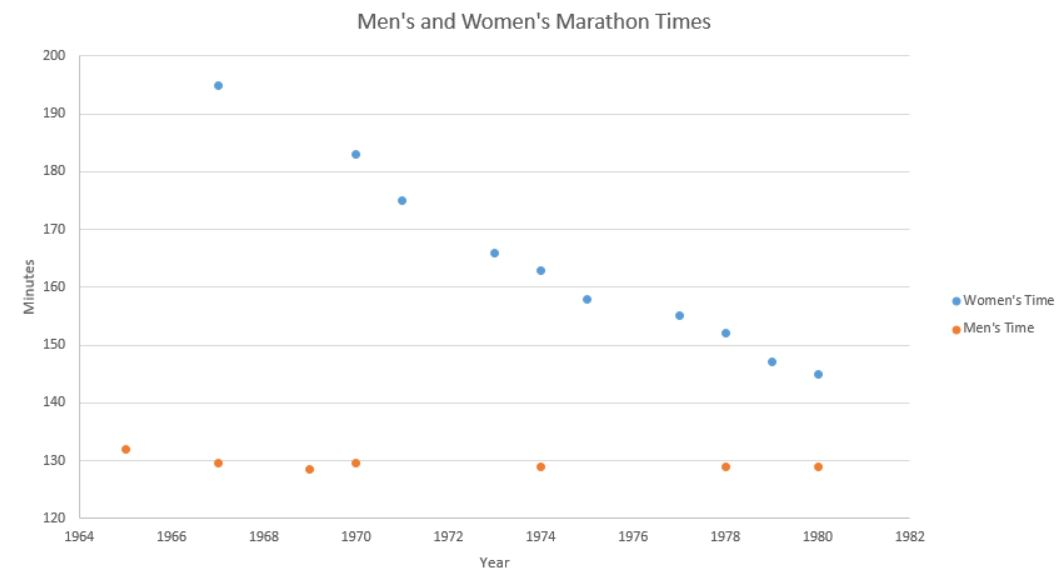
\includegraphics[width=\textwidth]{MarathonTimes1}
\end{center}
\pagebreak

From this data, it looks like both sets of data are following a linear trend.  If we use the first and last data points to find the average rate of change for each, we get the following linear models, using 1967 as $t=0$:
\begin{align*}
M_t &= 129.5-0.2t\\
W_t &= 195-3.85t
\end{align*}

According to these two linear models, we would predict that the women's record would beat the men's record by 1985; however, in 1985, the men's record was still 14 minutes faster than the women's.  What happened here?\\

Since women began setting marathon records about 50 years later than men, in the early years their progress was drastic, but eventually slowed down, and the trend was not linear over the long run (wow, what a terrible pun).\\

It should be clear that this linear trend was misleading, since if we extrapolated this model too far forward, we'd get ridiculous results.  The model predicts, for instance, that women would run the marathon in 1:20:00 in 1997 (a pace of about 20 mph, the speed of a roadrunner or close to the top speed of Usain Bolt at full sprint), or that by 2017 they'd be running it in 2.5 minutes (around 630 mph).
\end{example}

The lesson is simple, and hopefully obvious: linear trends are usually only useful in the short term; few phenomena follow linear trends over the long run.  That is why we'll examine other types of models in the coming sections.  However, keep this in mind, because we'll find that even those more sophisticated models have their limitations, and often they too break down in the long run.

\begin{exercises}
\ptwo{Marko currently has 20 tulips in his yard.  Each year he plants 5 more.
\begin{enumerate}[(a)]
\item Write a recursive formula for the number of tulips Marko has.
\item Write an explicit formula for the number of tulips Marko has.
\end{enumerate}
}
\ptwo{Pam is a DJ.  Every week she buys 3 new albums to add to her collection.  She currently owns 450 albums.
\begin{enumerate}[(a)]
\item Write a recursive formula for the number of albums Pam has.
\item Write an explicit formula for the number of albums Pam has.
\end{enumerate}
}

\ptwo{A store's sales (in thousands of dollars) grow according to the recursive rule $P_t = P_{t-1} + 15$, with initial sales $P_0 = 40$.
\begin{enumerate}[(a)]
\item Calculate $P_1$ and $P_2$.
\item Find an explicit formula for $P_t$.
\item Use the explicit formula to predict the store's sales in 10 years.
\item When will the store's sales exceed \$100,000?
\end{enumerate}
}
\ptwo{The number of houses in a town has been growing according to the recursive rule $P_t = P_{t-1} + 30$, with an initial number of $P_0 = 200$.
\begin{enumerate}[(a)]
\item Calculate $P_1$ and $P_2$.
\item Find an explicit formula for $P_t$.
\item Use the explicit formula to predict the number of houses in 10 years.
\item When will the number of houses reach 400?
\end{enumerate}
}

\ptwo{A population of beetles is growing according to a linear growth model.  The initial population (week 0) was $P_0=3$, and the population after 8 weeks is $P_8=67$.
\begin{enumerate}[(a)]
\item Find an explicit formula for the beetle population in week $t$.
\item After how many weeks will the beetle population reach 187?
\end{enumerate}
}
\ptwo{The number of streetlights in a town is growing linearly.  Four months ago ($t=0$) there were 130 lights.  Now ($t=4$) there are 146 lights.  If this trend continues,
\begin{enumerate}[(a)]
\item Find an explicit formula for the number of lights in month $t$.
\item How many months will it take to reach 200 lights?
\end{enumerate}
}
\end{exercises}


\section{Exponential Models}
\setcounter{ExampleCounter}{1}
As we saw with the last few examples in the previous section, linear models often break down over the long term; in fact, few natural phenomena actually follow linear trends, so at best linear models are usually just a rough short-term approximation.  On the other hand, many applications follow \textbf{exponential growth.}  One of the most common is population growth, so we'll use an example of that for illustration.

Suppose you're tracking the population of fish in a lake, and every year 10\% of the fish have surviving offspring.  Notice that this is still a simplified model, since more sophisticated models account for predators, limited resources, and so on.  In our simple model, though, an initial population of 1000 fish would grow to 1100 fish after the first year, and each subsequent year, 10\% of the population at that time will be added, so the population grows faster as it gets larger.

The recursive model is shown below.
\begin{align*}
P_0 &= 1000\\
P_t &= P_{t-1} + 0.10P_{t-1}
\end{align*}

We can use this to derive a closed-form model:
\begin{align*}
P_0 &= 1000\\
P_1 &= P_0 + 0.10P_0 = P_0(1+0.10) = P_0 \cdot 1.10\\
P_2 &= P_1 \cdot 1.10 = P_0 \cdot 1.10 \cdot 1.10 = P_0 \cdot 1.10^2\\
P_3 &= P_2 \cdot 1.10 = P_0 \cdot 1.10^3\\
&\vdots\\
P_t &= P_0 \cdot 1.10^t
\end{align*}

The \textbf{growth rate} is 10\%, and 1.10 is the \textbf{growth multiplier}.  Each year's population is 1.10 times the previous year's population.

\begin{center}
\begin{tabular}{c | c | c}
\textbf{Year} & \textbf{Population} & \textbf{Growth from Previous Year}\\
\hline
0 & 1000 &\\
1 & 1100 & 100\\
2 & 1210 & 110\\
3 & 1331 & 121\\
4 & 1464 & 133\\
5 & 1611 & 147\\
6 & 1772 & 161
\end{tabular}
\end{center}
Notice that there is a constant \textit{percentage} growth, so as the population increases, the number by which it grows gets larger each year.\\

If we plot these first few values, the graph is not quite linear, but it's not that far from a linear plot.  Because of this, in the short term, linear models can approximate exponential models, even if it isn't a perfect fit.
\begin{center}
\begin{tikzpicture}
\begin{axis}[
    xmin=0, xmax=6,
    ymin=800, ymax=2000,
    axis lines=center,
    axis on top=false,
    domain=0:1,
    x=1.6cm,
    y=0.004cm,
    xtick={0,1,...,6},
    xticklabels={0,1,...,6},
    ytick={0,200,...,2000},
    yticklabels={0,200,...,2000},
    axis lines=middle,
    axis line style={->},
    x label style={at={(axis description cs:0.5,-0.1)},anchor=north},
    y label style={at={(axis description cs:-0.1,.5)},rotate=90,anchor=south},
    xlabel={Years From Now},
    ylabel={Fish Population},
    grid=major
    ]
	\addplot [blue,only marks] table {
	0 1000
	1 1100
	2 1210
	3 1331
	4 1464
	5 1611
	6 1772
	};
\end{axis}
\end{tikzpicture}
\end{center}
%\begin{center}
%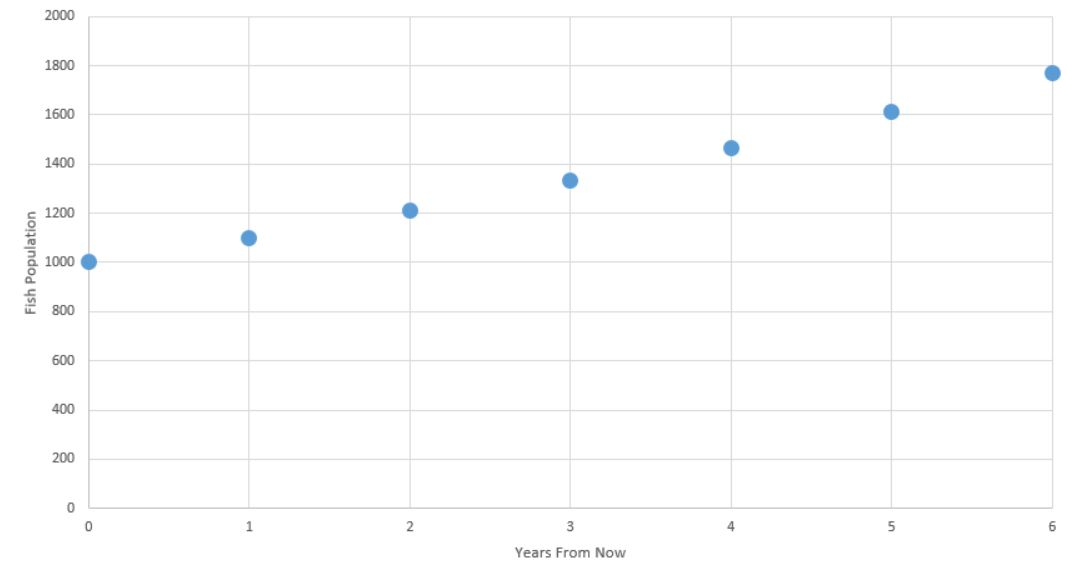
\includegraphics[width=0.7\textwidth]{ExpGrowthLinear}
%\end{center}
\vfill
\pagebreak

As we begin to project further into the future, though, the model clearly deviates from a linear trend:
\begin{center}
\begin{tikzpicture}
\begin{axis}[
    xmin=0, xmax=30,
    ymin=0, ymax=20,
    axis lines=center,
    axis on top=false,
    domain=0:1,
    x=0.32cm,
    y=0.4cm,
    xtick={0,5,...,30},
    xticklabels={0,5,...,30},
    ytick={0,2,...,20},
    yticklabels={0,{2,000},{4,000},{6,000},{8,000},{10,000},{12,000},{14,000},{16,000},{18,000},{20,000}},
    axis lines=middle,
    axis line style={->},
    x label style={at={(axis description cs:0.5,-0.1)},anchor=north},
    y label style={at={(axis description cs:-0.1,.5)},rotate=90,anchor=south},
    xlabel={Years From Now},
    ylabel={Fish Population},
    grid=major
    ]
	\addplot [blue,only marks] table {
	0 1
	1 1.1
	2 1.21
	3 1.331
	4 1.464
	5 1.611
	6 1.772
	7 1.949
	8 2.144
	9 2.358
	10 2.594
	11 2.853
	12 3.138
	13 3.452
	14 3.798
	15 4.177
	16 4.595
	17 5.055
	18 5.56
	19 6.116
	20 6.728
	21 7.4
	22 8.14
	23 8.954
	24 9.85
	25 10.835
	26 11.918
	27 13.11
	28 14.421
	29 15.863
	30 17.45
	};
\end{axis}
\end{tikzpicture}
\end{center}
%\begin{center}
%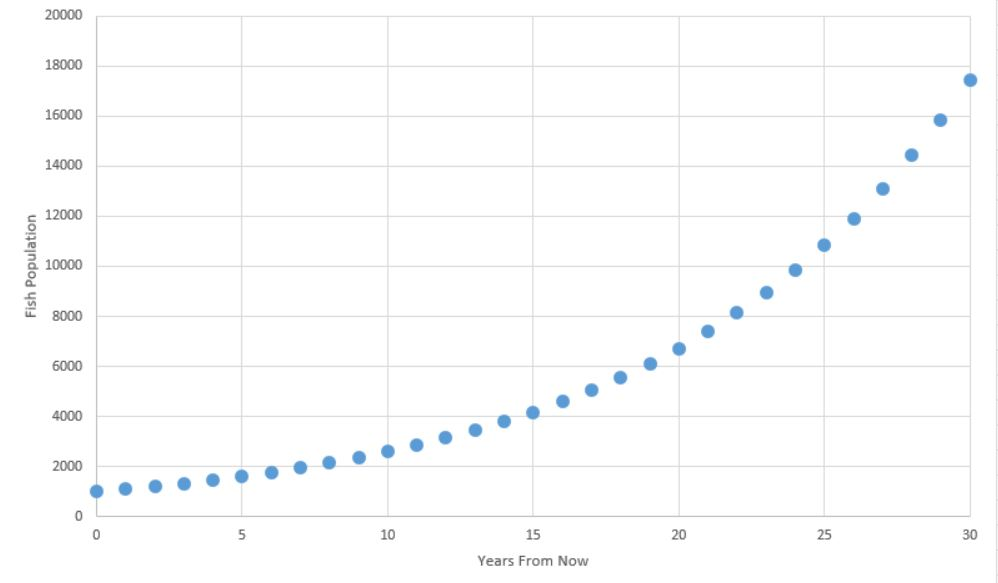
\includegraphics[width=0.7\textwidth]{ExpGrowthExponential}
%\end{center}

If the population had been growing linearly by 100 fish each year, the population at the end of 30 years would have only been 4000 instead of nearly 18,000 under the exponential model.  Most of this growth occurred in the second half; this is typical of exponential growth.  Since the growth from one year to another depends on the size of the population, it grows much faster near the end, and the growth begins to snowball.

\begin{formula}{Exponential Growth}
If a quantity starts at size $P_0$ and grows by $R\%$ (written as a decimal, $r$) every time period, then the quantity after $t$ time periods is given by
\[P_t = P_0 (1+r)^t\]
The \textbf{growth rate} is $r$, and the \textbf{growth multiplier} is $1+r$.

If $r$ is negative, then instead of exponential growth there is \textbf{exponential decay}.
\end{formula}

The growth multiplier is the common ratio between terms, and it can be used to recognize exponential growth from data, just like a common difference between terms can be used to recognize linear growth.
\begin{center}
\begin{tabular}{c | c | c}
\textbf{Year} & \textbf{Population} & \textbf{Ratio to Previous Year}\\
\hline
0 & 1000 &\\
1 & 1100 & 1.1\\
2 & 1210 & 1.1\\
3 & 1331 & 1.1\\
4 & 1464 & 1.1\\
5 & 1611 & 1.1\\
6 & 1772 & 1.1
\end{tabular}
\end{center}
\pagebreak

\begin{example}[https://www.youtube.com/watch?v=NHLi7ekPSPM]{Frederick Population}
The population of Frederick County grew from 239,520 in 2012 to 241,409 in 2013, a growth of about 0.8\%.  If this growth rate continues, what is the population of Frederick County expected to be in 2025?\\

\marginnote{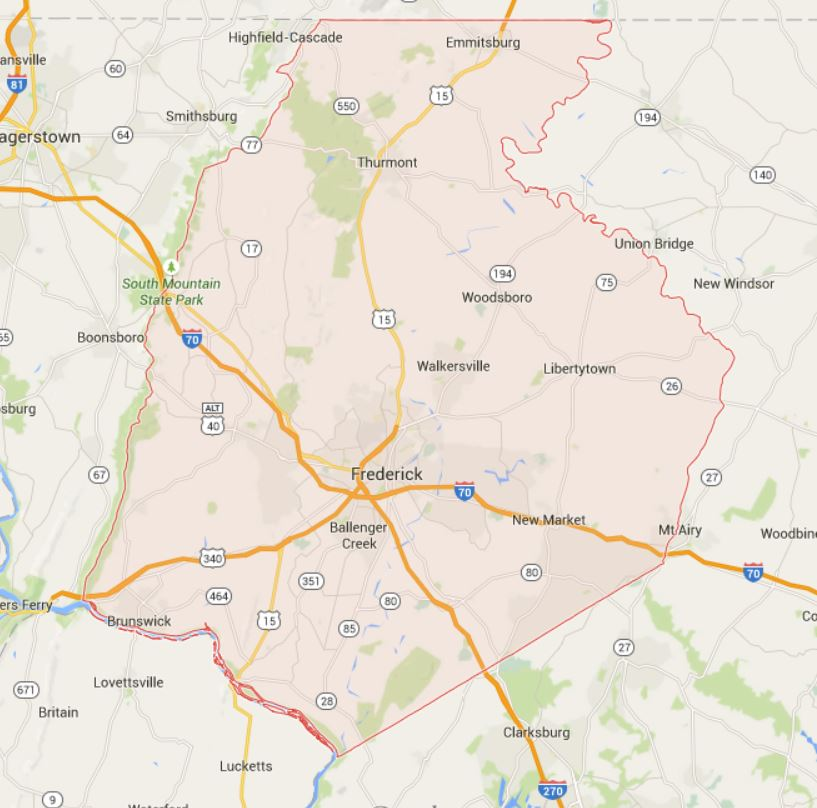
\includegraphics[scale=0.15]{FrederickCountyMap1}}
If $r=0.008$, we can use the exponential growth formula to predict the population in 2025.  To do so, however, we need to pick a year to be year 0.  Since we're given the population in 2012 and 2013, we can use either one, but we'll choose 2013, so 2025 will be year 12.
\begin{align*}
P_{12} &= P_0 (1+r)^t\\
&= 241,409(1+0.008)^{12}\\
&= 265,632
\end{align*}
We expect the population of Frederick County to reach 265,632 by 2025.
\end{example}

\begin{try}[http://www.izzomath.com/103text/growthmodels/example2.1/story.html]
\begin{tabular}{b{2in} c}
India is the second most populous country in the world, with a population of about 1.252 billion in 2013.  The population is growing by about 1.21\% each year.

If this trend continues, what is India's population expected to grow to by 2030? & 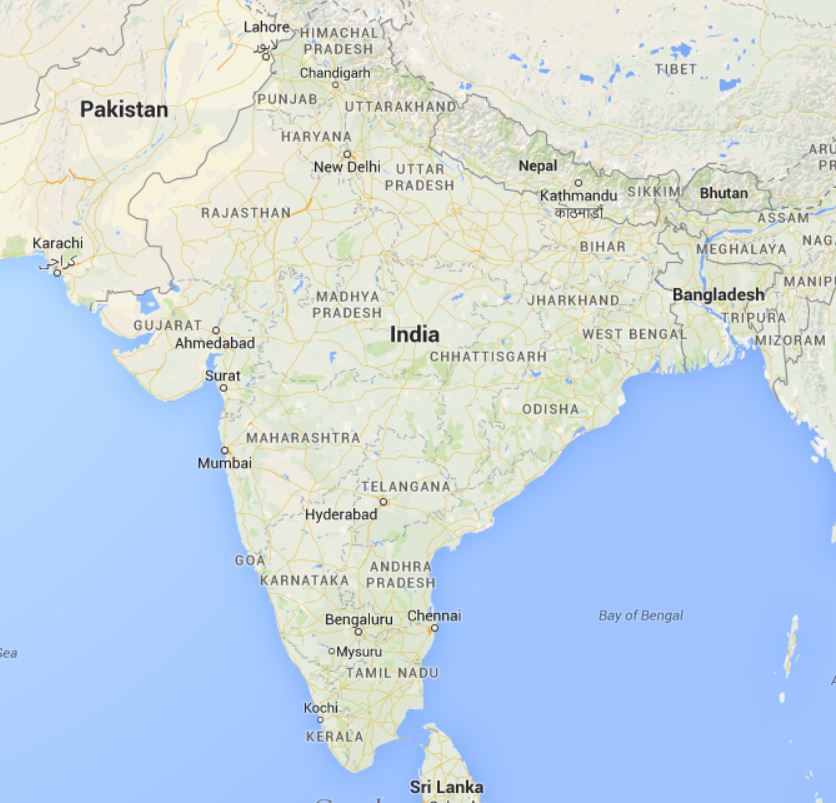
\includegraphics[width=0.5\textwidth]{IndiaMap1}
\end{tabular}
\end{try}

\begin{proc}{Using Your Calculator: Exponents}
\begin{tabular}{c l}
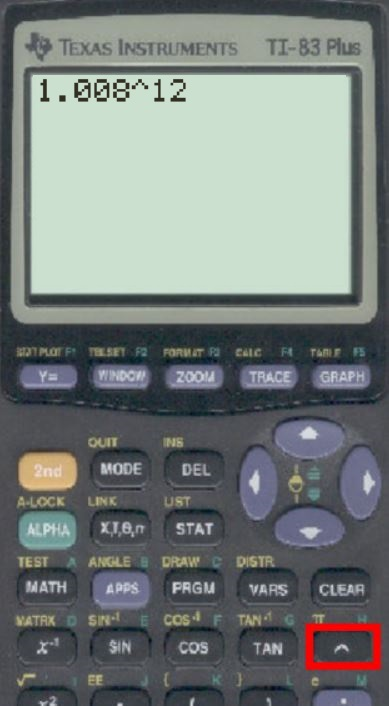
\includegraphics[scale=0.35]{Calculator2} & \parbox[b]{3in}{To evaluate expressions like $1.008^{12}$, we'll use the exponent function on a calculator rather than multiplying 1.008 by itself 12 times.  The exponent function is usually labeled like one of the following:
\begin{center}
\begin{tabular}{c c c}
$\boxed{\wedge}$ & $\boxed{y^x}$ & $\boxed{x^y}$
\end{tabular}
\end{center}

To evaluate $1.008^{12}$, we'd type $1.008 \ \boxed{\wedge}\ 12$ or $1.008\ \boxed{y^x}\ 12$.  Try it and make sure that you get an answer around 1.100338694.}
\end{tabular}
\end{proc}
\pagebreak

\begin{example}[https://www.youtube.com/watch?v=_u9RlZX_BkI]{Tuition Prediction}
A friend is using the equation \[P_t = 4600(1.072)^t\] to predict the annual tuition at a local college.  She says that the formula is based on years after 2010.  What does this equation tell us?\\

\marginnote{\bfseries Solution}
In this equation, $P_0 = 4600$, which is the initial tuition, so we infer that the tuition in 2010 is \$4600.

The growth multiplier is 1.072, so the growth rate is 0.072 or 7.2\%.  We expect tuition to grow by 7.2\% each year.
\end{example}

\begin{example}[https://www.youtube.com/watch?v=2wtJ_T3_e7o]{Carbon Dioxide Emissions}
In 1990, the residential energy use in the US was responsible for 962 million metric tons of carbon dioxide emissions.  By the year 2000, that number had risen to 1182 million metric tons.  If the emissions grow exponentially and continue at the same rate, what will the emissions grow to by 2050?\\

\marginnote{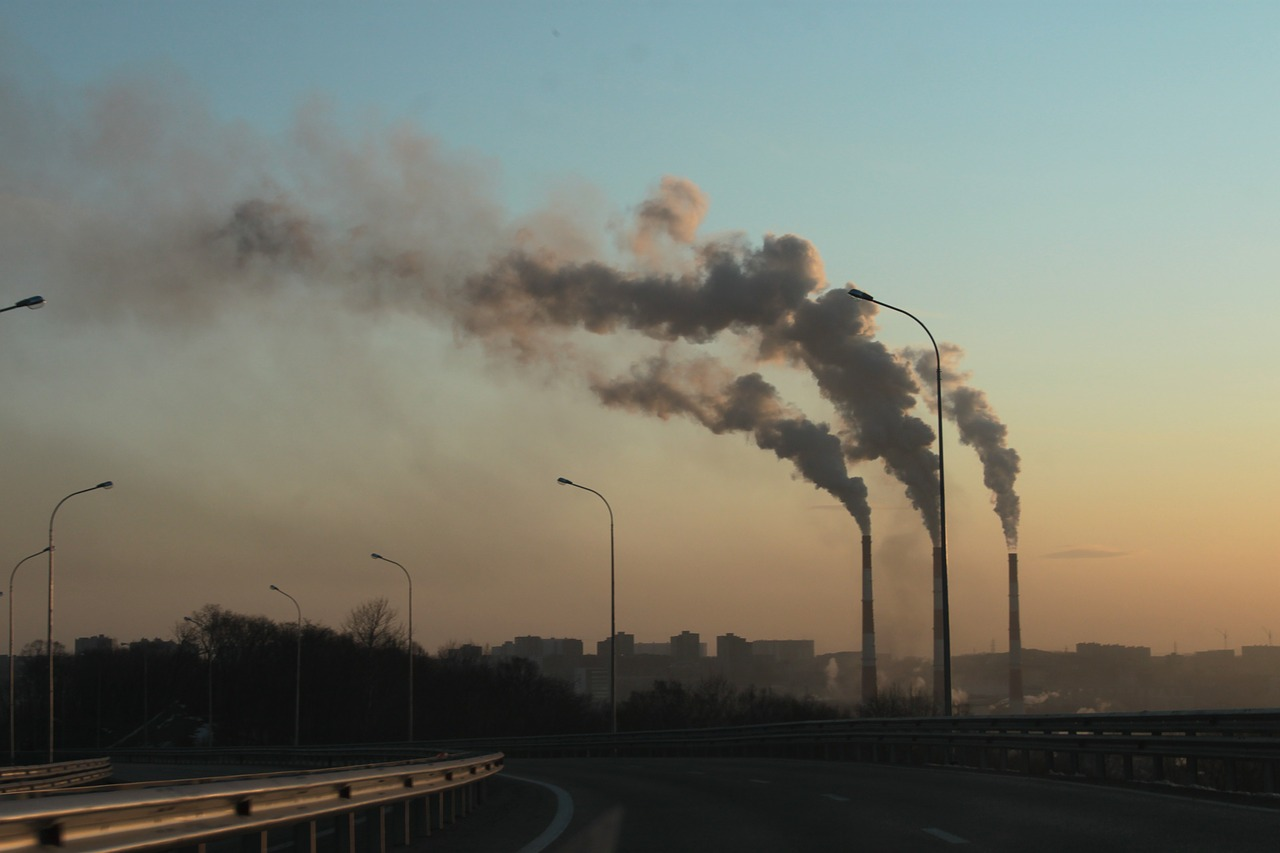
\includegraphics[scale=0.08]{Factory1}}
The twist in this problem is that the growth rate is not explicitly given, so we'll have to find it before we can make our prediction.

We will let 1990 correspond to year 0, so 2000 is year 10.
\begin{center}
\begin{tabular}{c c}
\textbf{Year} & \textbf{Emissions (million tons)}\\
\hline
0 & 962\\
10 & 1182
\end{tabular}
\end{center}
We can put this information into the exponential growth model:
\begin{align*}
P_{10} &= P_0(1+r)^{10}\\
1182 &= 962(1+r)^{10}
\end{align*}

Now we need to solve for $r$:
\begin{center}
\begin{tabular}{c l}
$1182 = 962(1+r)^{10}$ & Divide both sides by 962\\
& \\
$\dfrac{1182}{962} = (1+r)^{10}$ & Take the 10th root of both sides\\
& \\
$\sqrt[10]{\dfrac{1182}{962}} = 1+r$ & Subtract 1 from both sides\\
& \\
$\sqrt[10]{\dfrac{1182}{962}}-1 = r$ &
\end{tabular}
\end{center}
\[r=\sqrt[10]{\dfrac{1182}{962}}-1 = 0.0208 = 2.08\%\]

So if the emissions are growing exponentially, they are growing by about 2.08\% per year.  We can use this to predict the emissions in 2050, using 1990 as year 0:
\[P_{60} = 962(1+0.0208)^{60} = 2208.4 \textrm{ million metric tons of CO}_2 \textrm{ in 2050}\]
\end{example}

\begin{try}[http://www.izzomath.com/103text/growthmodels/example2.3/story.html]
The number of users on a social networking site was 45,000 in February when they officially went public, and grew to 60,000 by October.  If the site is growing exponentially and growth continues at the same rate, how many users should they expect two years after they went public?
\end{try}

\begin{proc}{Using Your Calculator: Roots}
In the previous example, we had to calculate the 10th root of a number.  Many scientific calculators have a button for general roots that looks like:
\begin{center}
\begin{tabular}{c c c}
$\boxed{\sqrt[n]{\hspace{0.1in}}}$ & $\boxed{\sqrt[x]{\hspace{0.1in}}}$ & $\boxed{\sqrt[y]{x}}$
\end{tabular}
\end{center}

To evaluate the 3rd root of 8, for example, we'd type either 3 $\boxed{\sqrt[n]{\hspace{0.1in}}}$ 8 or 8 $\boxed{\sqrt[n]{\hspace{0.1in}}}$ 3, depending on the calculator.  Try it on yours to see---you should get 2.\\

If you can't find a general root button, you can use the property of exponents that \[\sqrt[n]{a} = a^{1/n}.\]
To compute $\sqrt[3]{8}$, then, you could use the exponent key on your calculator to evaluate $8^{1/3}$.  Make sure that you use parentheses to preserve order of operations:
\[8\ \boxed{y^x}\ (\ 1\ \boxed{\div}\ 3\ )\]
\end{proc}

\paragraph{Rounding} If we had rounded the growth rate to 2.1\%, our calculation for the emissions in 2050 would have been 3347.  Rounding to 2\% would have given a result of 3156.  A very small difference in the growth rate gets magnified greatly in exponential growth.  Thus, round the growth rate as little as possible, keeping at least three significant digits (numbers after any leading zeros).  For instance, 0.41624 could be reasonably rounded to 0.416, and a growth rate of 0.001027 could be rounded to 0.00103.

\paragraph{Is the data linear or exponential?} So far in these examples, we've been told whether to use a linear model or an exponential one to make predictions, but the real world is not so accommodating; we often need to determine which kind of model we want to use.  To determine what kind of model will produce the best results, we can do a couple of things:
\begin{enumerate}
\item Plot data values from the past, as many as you can.  Look for a trend; does the data appear to be following a line, or does the curve look more like an exponential graph?  Keep in mind that in the short term, the difference is not that dramatic.
\item Think about the actual factors at play in the scenario; are they things you would expect to change linearly or exponentially?  For example, in the case of carbon emissions, we could expect that they might be tied closely to population values, which tend to change exponentially, since population growth is a percentage of the current population.
\end{enumerate}

\subsection{Exponential Growth with $e$}
What makes exponential growth exponential?  For instance, $1.005^t$ is exponential but $t^{1.005}$ is not, although there is an exponent in both.  The difference lies in where the variable $t$ is located---this is the quantity that varies in the model, and the one for which we want to predict results.  If the variable is in the \textit{base} of the exponent, it is not an exponential model, but only if the variable is in the \textit{exponent}.

We've seen several exponential models with different bases, but there is one base that is used more than any other: the natural base.\footnote{See the section on continuously compounded interest in the Financial Math chapter for more information.}  This is an irrational number (meaning it cannot be written as a fraction and its decimal form has digits after the decimal point that go on without end), and the letter $e$ is reserved for it: \[e = 2.71828 \ldots\]
It turns out that any exponential model, no matter the base, can be rewritten using the natural base, so if you encounter exponential models elsewhere, they may all be written with $e$ as the base.
\pagebreak

\begin{example}[https://www.youtube.com/watch?v=w8k-ob4i2U0]{US Population}
The population in the United States has been growing approximately according to the following exponential model since 1930:
\[P_t = 123.1e^{0.01217t}\]
where population is measured in millions.

Interpret this model and use it to predict the population in 2000.\\

\marginnote{\includegraphics[scale=0.1]{USPop1}}
If we let $t=0$ (1930), notice that $e^{(0.01217)(0)} = 1$ (remember, anything raised to 0 equals 1), so $P_0 = 123.1$.  Thus, we conclude that the population was 123.1 million in 1930, and the growth rate is 1.217\% (although growth rate means something slightly different than it did before we introduced $e$).\\

To predict the population in 2000, simply let $t=70$:
\[P_{70} = 123.1e^{(0.01217)(70)} = 288.5\]
This model predicts that the 2000 US population would be 288.5 million people, while the actual population in 2000 was 282.2 million.  Again, the model isn't perfect, but considering that we used it to predict a value 70 years in the future, it ended up performing pretty well.  Remember, the further we extrapolate, the worse our results will be.
\end{example}

\begin{try}[http://www.izzomath.com/103text/growthmodels/example2.4/story.html]
A colony of bacteria is growing exponentially according to the following model:
\[P_t = 1200e^{0.035t}\]
where $t$ is measured in weeks.
\begin{enumerate}
\item What was the initial population?
\item Use this model to predict the population after 7 weeks.
\end{enumerate}
\end{try}

\subsection{Radioactive Decay}
So far, all of the examples have featured exponential \textit{growth}, meaning that the values increased over time.  However, there are times where we may study quantities that \textit{decrease} over time according to an exponential model.  We'll use the natural base for the exponential models here.

In an exponential model like
\[P_t = P_0 e^{kt}\]
$k$ is called the growth rate.  As $t$ gets larger, $e^{kt}$ gets larger as well, and the quantity grows.  However, if we want to talk about exponential \textit{decay}, where the quantity is decreasing, what should we change?

Since $k$ is called the growth rate, we might think to start there.  In all of the examples we've seen so far, $k$ has been positive.  What if we make it negative?  To ask that another way, what happens when we raise $e$ to a negative number?  Do we get a negative result?

It may help to remember an exponent rule: $x^{-a} = \dfrac{1}{x^a}$

Thus,
\begin{align*}
e^{-1} &= \dfrac{1}{e^1} \approx 0.368\\
e^{-2} &= \dfrac{1}{e^2} \approx 0.135\\
e^{-3} &= \dfrac{1}{e^3} \approx 0.050\\
e^{-4} &= \dfrac{1}{e^4} \approx 0.018\\
\end{align*}
and you begin to see the trend.  If $k$ is negative, the exponent will be negative, making $e^{kt}$ smaller as $t$ increases, meaning that the total quantity $P_t$ will decrease as $t$ increases.  This is exponential decay.

\begin{formula}{Exponential Growth and Decay}
\marginnote{\footnotesize Note that although $k$ is also called a growth rate, it belongs to a different model than the earlier growth rate $r$}
Consider a general exponential model
\[P_t = P_0 \ e^{kt}\]

If $k$ is positive, it is called the \textbf{growth rate}, and $P_t$ increases as $t$ increases.

If $k$ is negative, it is called the \textbf{decay rate}, and $P_t$ decreases as $t$ increases.
\end{formula}

\begin{example}[https://www.youtube.com/watch?v=6SIiItzYfQo]{Radioactive Decay}
Radioactive gold 198, used in imaging the structure of the liver, decays exponentially according to the following model:
\[A_t = A_0 \ e^{-0.2596t}\] where $t$ is measured in days.  If we start with 50 milligrams of the isotope, how many milligrams will be left after a week?\\

\marginnote{\bfseries Solution}
Simply let $t=7$:
\[A_7 = 50e^{-0.2596(7)} = 8.12 \textrm{ milligrams}\]
As expected, there is less after a week than we started with.
\end{example}

\begin{try}[http://www.izzomath.com/103text/growthmodels/example2.5/story.html]
The atmospheric pressure $p$ on a plane decreases with increasing height.  This pressure, measured in mmHg, is related to the height $h$ in km above sea level by the model $p=760e^{-0.145h}$  Find the atmospheric pressure at a height of 2 km above sea level.
\end{try}

\subsection{Using Logarithms to Solve for Time}
At the beginning of this section, we modeled the population growth of Frederick County from 2013 onward using the following equation:
\vspace{0.1in}
\[P_t = 241,409(1+0.008)^t\]
\vspace{0.1in}

We can use this equation to predict the population at any point in the future (albeit imperfectly) if we have a year that we're interested in.  What if we flip the problem around, though?  What if, instead of being given a year and asked to find the population, we were interested in knowing what year the population hit a certain mark? \\ 

For instance, what if we wanted to know when the population of Frederick County would reach 400,000?  Here $P_t$ is given and $t$ is what we're looking for:
\vspace{0.1in}

\begin{center}
\begin{tabular}{r @{ $=$ } l l}
400,000 & $241,409(1.008)^t$ & Divide both sides by 241,409\\
1.657 & $1.008^t$ & We need to solve this for $t$
\end{tabular}
\end{center}
\vfill
\pagebreak

One way to make this prediction would be to create a table of values, or draw a graph using a computer or graphing calculator.
\begin{center}
\begin{tikzpicture}
\begin{axis}[
    xmin=-1, xmax=70,
    ymin=0, ymax=450,
    axis lines=center,
    axis on top=true,
    domain=0:1,
    x=0.15cm,
    y=0.015cm,
    xtick={0,5,...,100},
    xticklabels={0,5,...,100},
    ytick={0,50,...,450},
    yticklabels={0,50,...,450},
    axis lines=middle,
    axis line style={->},
    x label style={at={(axis description cs:0.5,-0.1)},anchor=north},
    y label style={at={(axis description cs:-0.1,.5)},rotate=90,anchor=south},
    xlabel={$t$ (Years after 2013)},
    ylabel={Population (Thousands)},
    grid=major
    ]
	\addplot[samples=100,domain=0:70] {241*(1.008^x)};
\end{axis}
\end{tikzpicture}
\end{center}

From the graph, we can estimate that the population will reach 400,000 somewhere between 60 and 65 years after 2013 (2073 to 2078), but we can do better than this.  To get a more precise answer, we turn to an algebraic tool known as the \textbf{logarithm}.

Today\footnote{Before computers were ubiquitous, logarithms were used to make hand calculations easier, especially useful when creating huge tables of navigational data}, one of the two main uses of logarithms is to solve equations like this one where the unknown lies in the exponent.  Just like a square root undoes a square, freeing the variable:
\[x^2 \longrightarrow \sqrt{x^2} = x\]
a logarithm undoes an exponential, freeing the variable from the exponent:
\[10^x \longrightarrow \log_{10} (10^x) = x\]

Each base has a logarithm to go with it, so to isolate the variable in $3^x$, we'd use $\log_3$, for $7^x$ we'd use $\log_7$, and so on.  We'll focus on two in particular, though: $\log_{10}$, which is abbreviated $\log$, and $\log_e$, which is abbreviated $\ln$ (meaning natural log)\footnote{From the Latin \textit{logarithmus naturalis}}.  These are the two that are easily accessible on most calculators, and all other logarithms can be calculated using either of these two.

\begin{formula}{The Common and Natural Logarithm}
The \textbf{common logarithm}, written $\log (x)$, undoes the exponential $10^x$:
\[\log(10^x) = x \textrm{ and } 10^{\log(x)} = x\]

The \textbf{natural logarithm}, written $\ln (x)$, undoes the exponential $e^x$:
\[\ln(e^x) = x \textrm{ and } e^{\ln(x)} = x\]

Any other logarithm can be written in terms of either of these by using the \textbf{change of base formula}:
\[\log_b(x) = \dfrac{\log(x)}{\log(b)} \textrm{ or } \log_b(x) = \dfrac{\ln(x)}{\ln(b)}\]
\end{formula}
\pagebreak

Before we begin using logarithms to solve equations like the one in the population example, let's get some practice with them.

\begin{example}[https://www.youtube.com/watch?v=_OTEHIGS3qM]{Common Logarithm}
Evaluate each of the following:
\begin{center}
\begin{tabular}{l l l l l}
(a) $\log(100)$ & (b) $\log(1000)$ & (c) $\log(10,000)$ & (d) $\log\left(\dfrac{1}{100}\right)$ & (e) $\log(1)$
\end{tabular}
\end{center}

\marginnote{\bfseries Solution}
\begin{enumerate}[(a)]
\item $\log(100)$ can be written as $\log\left(10^2\right) = 2$
\item $\log(1000) = \log\left(10^3\right) = 3$
\item $\log(10,000) = \log\left(10^4\right) = 4$
\item Recall that $x^{-n} = \dfrac{1}{x^n}$, so $\log\left(\dfrac{1}{100}\right) = \log\left(10^{-2}\right) = -2$
\item Recall that $x^0=1$, so $\log(1) = \log\left(10^0\right) = 0$
\end{enumerate}
\end{example}

\begin{try}[http://www.izzomath.com/103text/growthmodels/example2.6/story.html]
Evaluate each of the following:
\begin{center}
\begin{tabular}{l l l l l}
(a) $\ln(e)$ & (b) $\ln(e^2)$ & (d) $\ln\left(\dfrac{1}{e^3}\right)$ & (e) $\ln(1)$
\end{tabular}
\end{center}
\end{try}

What if the number we're trying to evaluate with a logarithm can't be written as a power of 10 or $e$?  For this, our calculator comes to the rescue.

\begin{proc}{Using Your Calculator: Logarithms}
\begin{center}
\begin{tabular}{l b{3in}}
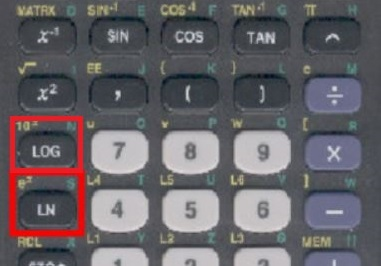
\includegraphics[scale=0.3]{CalculatorLog} & Look for buttons labeled LOG and LN on your calculator.  Try the answers in the example above to check yourself.
\end{tabular}
\end{center}
\end{proc}

\begin{example}[https://www.youtube.com/watch?v=AE02zNX0nVg]{Evaluating Logarithms with a Calculator}
Evaluate each of the following with a calculator:
\begin{center}
\begin{tabular}{l l l l}
(a) $\log(300)$ & (b) $\log(4.5)$ & (c) $\ln(31)$ & (d) $\ln(0.1)$\\
\marginnote{\bfseries Solution}
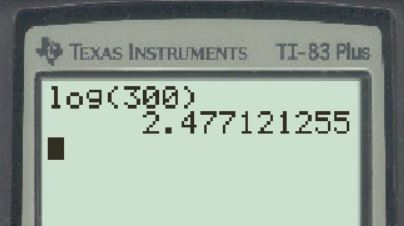
\includegraphics[height=0.6in]{CalculatorLog300} & 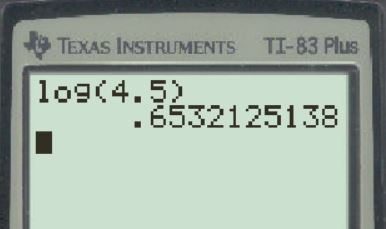
\includegraphics[height=0.6in]{CalculatorLog45} & 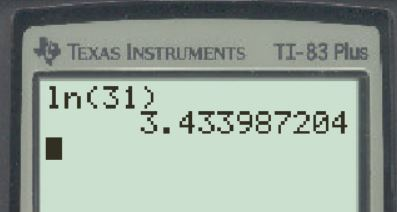
\includegraphics[height=0.6in]{CalculatorLn31} & 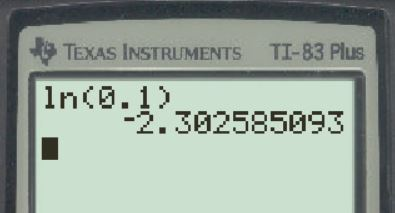
\includegraphics[height=0.6in]{CalculatorLn01}\\
2.477 & 0.653 & 3.434 & $-2.303$
\end{tabular}
\end{center}
\end{example}

\begin{try}[http://www.izzomath.com/103text/growthmodels/example2.7/story.html]
Evaluate each of the following with a calculator:
\begin{center}
\begin{tabular}{l l l l}
(a) $\log(0.5)$ & (b) $\log(27)$ & (c) $\ln(2)$ & (d) $\ln(0.85)$
\end{tabular}
\end{center}
\end{try}
\pagebreak

What about something like $\log_5(30)$?  Can we use our calculator to evaluate this?  Some calculators have a function for logarithms with any base, but if they do, it's buried in a menu somewhere.  Instead, we'll use the change-of-base formula, since that only requires using either the LOG key or the LN key, which most calculators have.
\[\log_5(30) = \dfrac{\log(30}{\log(5)} = \dfrac{1.477}{0.699} = 2.113\]

Notice that if we used the change-of-base formula with LN instead, we'd get the same answer:
\[\log_5(30) = \dfrac{\ln(30}{\ln(5)} = \dfrac{3.401}{1.609} = 2.113\]

Thus, you can use the change-of-base formula with either LOG or LN to evaluate logarithms with any base.

\begin{try}
Evaluate each of the following with a calculator:
\begin{center}
\begin{tabular}{l l l l}
(a) $\log_3(12)$ & (b) $\log_{1.5}(99)$ & (c) $\log_{0.7}(3)$ & (d) $\log_{23}(1.77)$
\end{tabular}
\end{center}
\end{try}

Now we finally get to the point of this: solving exponential equations using logarithms.  Remember that the key to solving equations in general is that whatever we do to one side, we must do to the other.  Just like we can add anything to both sides or square both sides, we can also take the logarithm of both sides of an equation and end up with an equivalent equation.  Since logarithms undo exponentials, this will simplify an equation that has a variable in the exponent.

\begin{example}[https://www.youtube.com/watch?v=JnA4ypiJB6g]{Solving Equations with Logarithms}
Solve each of the following equations:
\begin{center}
\begin{tabular}{l l l l}
(a) $10^x=1000$ & (b) $10^x=3$ & (c) $2(10^x)=8$ & (d) $e^x=5$\\
(e) $3e^x=12$ & (f) $2.5^x=17$ & (g) $0.2^x=2$ & (h) $50(1.04^x)=125$
\end{tabular}
\end{center}

\marginnote{\bfseries Solution}
\begin{enumerate}[(a)]
\item Take the log of both sides: \[\log(10^x) = \log(10^3) \longrightarrow x=3\]
\item Take the log of both sides: \[\log(10^x) = \log(3) \longrightarrow x=\log(3) \approx 0.477\]
\item Isolate the exponential before taking the log of both sides:
\[2(10^x)=8 \longrightarrow 10^x = 4 \longrightarrow x=\log(4) \approx 0.602\]
\item Use the natural log this time:
\[e^x=5 \longrightarrow \ln(e^x) = \ln(5) \longrightarrow x=\ln(5) \approx 1.609\]
\item Again, isolate the exponential, and use the natural log:
\[3e^x = 12 \longrightarrow e^x=4 \longrightarrow x=\ln(4) \approx 1.386\]
\item Here we have to use the change-of-base formula:
\[2.5^x=17 \longrightarrow \log_{2.5}(2.5^x)=\log_{2.5}(17) \longrightarrow x = \dfrac{\log(17)}{\log(2.5)} \approx 3.092\]
\item Again, using the change-of-base formula:
\[0.2^x = 2 \longrightarrow x=\log_{0.2}(2) = \dfrac{\log(2)}{\log(0.2)} \approx -0.4307\]
\item Isolate the exponential before using the change-of-base formula:
\[50(1.04^x) = 125 \longrightarrow 1.04^x = 2.5 \longrightarrow x = \log_{1.04}(2.5) = \dfrac{\log(2.5)}{\log(1.04)} \approx 23.36\]
\end{enumerate}
\end{example}
\pagebreak

\begin{try}[http://www.izzomath.com/103text/growthmodels/example2.8/story.html]
Solve each of the following equations:
\begin{center}
\begin{tabular}{l l l l}
(a) $10^x=4$ & (b) $5e^x=8$ & (c) $2^x=75$ & (d) $20(1.95^x)=140$
\end{tabular}
\end{center}
\end{try}

Now that we can use logarithms to solve exponential equations with any base, we can return to our discussion of the population model for Frederick County.  Recall that we have the model
\[P_t = 241,409(1.008^t)\]
and we asked when the population would reach 400,000, which led to the equation \[1.657=1.008^t\] where we want to solve for $t$.  Now we know how to do this:
\[1.008^t=1.657 \longrightarrow t = \log_{1.008} (1.657) = \dfrac{\log(1.657)}{\log(1.008)} \approx 63.4\]
We conclude that according to this model, the population of Frederick County will reach 400,000 about 63 years after 2013, or the year 2076.

\begin{example}[https://www.youtube.com/watch?v=ei5RaBwgRNc]{Filtering Water}
Polluted water is passed through a series of filters.  Each filter removes 90\% of the remaining impurities from the water.  If you have 10 million particles of pollutant per gallon originally, how many filters would the water need to be passed through to reduce the pollutant to 500 particles per gallon?\\

\marginnote{\includegraphics[scale=0.15]{ROFilter}\\\footnotesize\textcolor{black!60}{From Wikipedia}\\\footnotesize\textcolor{black!60}{Photo by Twhair}}
In this problem, our ``population'' is the number of particles of pollutant per gallon.  The initial pollutant is 10 million particles per gallon, so \[P_0 = 10,000,000.\]  Instead of changing with time, the population changes with the number of filters, so $t$ will represent the number of filters used.

Since the amount of pollutant is decreasing with each filter, this is an example of exponential decay, with a decay rate of $r=-0.90$.

The decay model is
\[P_t = 10,000,000(1-0.90)^t = 10,000,000(0.1^t).\]

To answer the question of how many filters are needed to lower the pollutant to 500 particles per gallon, we set $P_t$ to 500 and solve for $t$:
\begin{center}
\begin{tabular}{r @{ $=$} l l}
500 & $10,000,000(0.1^t)$ & Divide both sides by 10,000,000\\
0.00005 & $0.1^t$ & Take the $\log_{0.1}$ of both sides\\
$\log_{0.1}(0.00005)$ & $t$ & Use the change-of-base formula\\
$\dfrac{\log(0.00005)}{\log(0.1)}$ & $t$ & Approximate with a calculator\\
4.301 & $t$
\end{tabular}
\end{center}
It would take about 4.301 filters to reduce the pollutant to the desired level, but since we can't install 0.3 filters, we would need to use 5 filters to reach the goal.
\end{example}

\begin{try}[http://www.izzomath.com/103text/growthmodels/example2.9/story.html]
India had a population in 2008 of about 1.14 billion people, growing by about 1.34\% each year.  If this trend continued, when was India's population expected to reach 1.2 billion?
\end{try}
\vfill
\pagebreak

\subsection{Application: Newton's Law of Cooling}
If you leave a hot cup of coffee out on the counter, you expect it to cool over time as it loses heat to the environment, or the \textit{medium}.  The rate at which this heat transfer occurs depends on many things, like the composition of the fluid, the humidity of the air, the materials of the coffee cup and the counter, and so on.  However, the most significant factor that controls this rate is the difference in temperature between the coffee cup and the environment; when the coffee is much hotter than the air around it, it will cool much more rapidly than when its temperature is closer to that of the air.  Over time, the coffee will approach room temperature and the transfer of heat will slow down.  Specifically, the temperature will decrease according to the equation \[T=T_m+(T_0-T_m)e^{kt}\] where $T$ is the temperature of the object (changing over time), $T_m$ is the temperature of the medium (the surroundings), $T_0$ is the initial temperature of the object (e.g. the coffee cup), and $k$ is the decay rate--a negative constant that depends on all of those other factors related to the environment and the materials.  This model also works if the object is cooler than the environment and warming over time, like if you placed a cup of ice water on the counter instead.\\

For example, suppose a coffee cup at 180$^{\circ}$ F is allowed to cool in a room whose air temperature is 65$^{\circ}$ F.
\begin{enumerate}
\item If the temperature of the cup is 120$^{\circ}$ F after 10 minutes, what is $k$?\\

Plug the given information into the equation and use logarithms to solve for $k$:
\begin{align*}
T &= T_m+(T_0-T_m)e^{kt}\\
120 &= 65 + (180-65)e^{k(10)}\\
55 &= 115e^{10k}\\
0.478 &= e^{10k}\\
\ln(0.478) &= 10k\\
-0.7376 &= 10k\\
-0.0738 &= k
\end{align*}

\item What will its temperature be after 20 minutes?\\

Let $t=20$ in the model, since now we know $k$:
\[T=65+(180-65)e^{-0.0738(20)} = 91.3\]
Thus we expect it to reach about 91$^{\circ}$ F after 20 minutes.

\item When will it reach 80$^{\circ}$ F?\\

Let $T=80$ and solve for $t$ using a logarithm:
\begin{align*}
80 &= 65+115e^{-0.0738t}\\
15 &= 115e^{-0.0738t}\\
0.1304 &= e^{-0.0738t}\\ 
-0.0738t &= \ln(0.1304)\\ 
t &\approx 27.6
\end{align*}
We expect the coffee cup to reach 80$^{\circ}$ F after about 28 minutes.
\pagebreak

\item Graph the temperature over time.
\begin{center}
\begin{tikzpicture}
\begin{axis}[
    xmin=-1, xmax=70,
    ymin=0, ymax=200,
    axis lines=center,
    axis on top=true,
    domain=0:1,
    x=0.15cm,
    y=0.03cm,
    xtick={0,5,...,100},
    xticklabels={0,5,...,100},
    ytick={0,25,...,200},
    yticklabels={0,25,...,200},
    axis lines=middle,
    axis line style={->},
    x label style={at={(axis description cs:0.5,-0.1)},anchor=north},
    y label style={at={(axis description cs:-0.1,.5)},rotate=90,anchor=south},
    xlabel={$t$ (Minutes)},
    ylabel={Temperature ($^{\circ}$ F)},
    grid=major
    ]
	\addplot[samples=100,domain=0:70] {65+115*e^(-0.0738*x)};
	\addplot[samples=100,domain=0:70,dashed] {65};
\end{axis}
\end{tikzpicture}
\end{center}

Notice the exponential shape of the curve, and notice that it predicts what we expected, that the temperature approaches 65$^{\circ}$ F over time; we call that behavior \textit{asymptotic}, since as $t$ gets larger, the temperature approaches 65 but never crosses below that.  As we noted, the rate of decrease is much larger at first, when the temperature difference is large, but it slows as the coffee's temperature gets closer to the room temperature.
\end{enumerate}

\begin{exercises}
\textit{In Exercises 1---8, evaluate each logarithm.}

\pfour{$\log(10)$}
\pfour{$\ln(e)$}
\pfour{$\log(23)$}
\pfour{$\ln(50)$}

\pfour{$\log\left(\dfrac{1}{1000}\right)$}
\pfour{$\ln\left(\dfrac{1}{e^5}\right)$}
\pfour{$\log_{1.5}(42)$}
\pfour{$\log_{0.57}(18)$}

\textit{In Exercises 9---16, solve each exponential equation.}

\pfour{$10^x=100$}
\pfour{$10^x=5$}
\pfour{$e^x=8$}
\pfour{$e^{2x}=19$}

\pfour{$4(10^x)=9$}
\pfour{$7^x=100$}
\pfour{$9(3^{2x})=56$}
\pfour{$22e^{0.05x}=37$}

\ptwo{Tacoma's population in 2000 was about 200 thousand, and had been growing by about 9\% per year.
\begin{enumerate}[(a)]
\item Write an explicit formula for the population of Tacoma.
\item If this trend continues, what will Tacoma's population be in 2016?
\item When does this model predict Tacoma's population to exceed 400 thousand?
\end{enumerate}}
\ptwo{Portland's population in 2007 was about 568 thousand, and had been growing by about 1.1\% per year.
\begin{enumerate}[(a)]
\item Write an explicit formula for the population of Portland.
\item If this trend continues, what will Portland's population be in 2016?
\item When does this model predict Portland's population to reach 700 thousand?
\end{enumerate}}

\ptwo{Diseases tend to spread exponentially.  In the early days of AIDS, the growth rate was around 190\%.  In 1983, about 1700 people in the US died of AIDS.  If the trend had continued unchecked, how many people would have died from AIDS in 2005?}
\ptwo{The population of the world in 1987 was 5 billion and the annual growth rate was estimated at 2 percent.  If the world population followed an exponential growth model, find the projected world population in 2015.}

\ptwo{A bacteria culture is started with 300 bacteria.  After 4 hours, the population has grown to 500 bacteria.  If the population grows exponentially according to the formula $P_t = P_0(1+r)^t$,
\begin{enumerate}[(a)]
\item Find the growth rate $r$ and write the full formula.
\item If this trend continues, how many bacteria will there be in one day?
\item How long will it take for this culture to triple in size?
\end{enumerate}}
\ptwo{A native wolf species has been reintroduced into a national forest.  Originally 200 wolves were transplanted, and after 3 years, the population had grown to 270 wolves.  If the population grows exponentially according to the formula $P_t = P_0(1+r)^t$,
\begin{enumerate}[(a)]
\item Find the growth rate $r$ and write the full formula.
\item If this trend continues, how many wolves will there be in ten years?
\item If this trend continues, how long will it take the population to grow to 1000 wolves?
\end{enumerate}}

\ptwo{The population in millions of the state of New Jersey has grown since 1973 according to the model $P_t=7.333e^{0.004t}$.
\begin{enumerate}[(a)]
\item What was the population of New Jersey in 1973?
\item What does this model predict the population of New Jersey would be in 1993?
\item According to this model, when will the population of New Jersey reach 9 million?
\end{enumerate}}
\ptwo{The population in millions of Colombia has grown since 1990 according to the model $P_t=33.31e^{0.018t}$.
\begin{enumerate}[(a)]
\item What was the population of Colombia in 1990?
\item What does this model predict the population of Colombia would be in 2000?
\item According to this model, when will the population of Colombia reach 52 million?
\end{enumerate}}

\ptwo{Strontium 90 is a radioactive isotope that decays according to the equation $A_t = A_0e^{-0.0244t}$, where $A_0$ is the initial amount present and $A_t$ is the amount present after $t$ years.  If you begin with 500 grams of strontium 90,
\begin{enumerate}[(a)]
\item How much strontium 90 will be left after 10 years?
\item When will 400 grams of strontium 90 be left?
\end{enumerate}}
\ptwo{Thorium 234 is a radioactive isotope that decays according to the equation $A_t = A_0e^{-10.498t}$, where $A_0$ is the initial amount present and $A_t$ is the amount present after $t$ years.  If you begin with 1000 grams of thorium 234,
\begin{enumerate}[(a)]
\item How much thorium 234 will be left after 0.5 years?
\item When will 250 grams of thorium 234 be left?
\end{enumerate}}

\ptwo{A hot bar of iron at 1,100$^{\circ}$ F is quenched in oil at 350$^{\circ}$ F.  After 2 minutes, the temperature of the iron is 750$^{\circ}$ F.
\begin{enumerate}[(a)]
\item Find the value for $k$ in Newton's Law of Cooling.
\item What will the temperature of the iron be after 10 minutes?
\item How long will it take for the iron to reach 400$^{\circ}$ F?
\end{enumerate}}
\ptwo{A frozen hot dog at $-32^{\circ}$ F is placed in a room at 70$^{\circ}$ F.  After 15 minutes, the temperature of the hot dog is 30$^{\circ}$ F.
\begin{enumerate}[(a)]
\item Find the value for $k$ in Newton's Law of Cooling.
\item What will the temperature of the hot dog be after 45 minutes?
\item How long will it take for the hot dog to reach 60$^{\circ}$ F?
\end{enumerate}}

\end{exercises}


\section{Logistic Models}
\setcounter{ExampleCounter}{1}
We can do better than exponential population growth models.  Why do we need to?  Aren't they good enough?  We'll illustrate with the world's population.  In 1950, the world population was 2.53 billion, and it grew to 5.32 billion by 1990, 40 years later.  We can use these two data points to build an exponential model:
\begin{align*}
P_t &= P_0 (1+r)^t\\
5.32 &= 2.53(1+r)^{40}\\
2.103 &= (1+r)^{40}\\
1.0188 &= 1+r\\
0.0188 &= r
\end{align*}
This gives us the model that predicts that $t$ years from 1950, the world population in billions will be \[P_t = 2.53(1.0188^t)\]

Let's test the model; let $t=55$, for example, corresponding to the year 2005.  The actual population in 2005 was 6.51 billion, and the model predicts that the population would be 7.03 billion.  Not perfect, but not terrible either.

However, what about 2015?  The model predicts 8.47 billion, and the actual population is only 7.32 billion.  In other words, the model is getting worse, and it's consistently overestimating; in 2005 the estimate was only off by half a billion, but by 2015 the error has more than doubled.  What's happening?

It turns out that the population growth rate is not constant, as the exponential model assumed.  Instead, the growth rate is slowing.  The world population grew from 1.60 billion in 1900 to 6.13 billion in 2000, so even if it grew by the same \textit{amount} (not even the same \textit{rate}, which would lead to even bigger numbers) we might naively assume that by 2100 the world population would top 11 billion.  However, the United Nations estimates that the population will top 8 billion around 2050, and then \textit{fall} back to around present-day levels by 2100.

What's going on here?  Well, there are many factors, including the development of poorer countries around the world (economists point out that the single most powerful factor in reducing birth rates is prosperity in a nation), but it also has to do with \textbf{limited resources}.  Clearly, the population can't keep growing forever without bound; the earth cannot sustain a trillion people, for instance, given current technology, infrastructure, and access to food and water.  This leads to our conclusion:
\begin{center}
Exponential models are not good enough in the long term\\ because they don't account for limited resources.
\end{center}

In the short term, exponential models can give decent estimates, but in the long run, they'll eventually give unsustainable results.  To account for this, we turn to \textbf{logistic models}, which do account for limited resources.
\vfill

\begin{proc}{Carrying Capacity}
The \textbf{carrying capacity}, or \textbf{maximum sustainable population}, is the largest population that an environment can support.
\end{proc}

\begin{formula}{Logistic Growth}
If a population is growing in a constrained environment with carrying capacity $M$ and growth rate $r$, then the population can be described by the logistic growth model:
\[P_t = \dfrac{M}{1+\left(\dfrac{M}{P_0}-1\right)e^{-rt}}\]
\end{formula}
\pagebreak

This model of population growth is sometimes called the \textit{Verhulst model}, after Pierre-Fran\c cois Verhulst, a Belgian mathematician who published the model in 1838\footnote{It was rediscovered and re-derived several times over the following centuries by other mathematicians studying population growth.} and used it in 1840 to predict the population of the U.S. up to 1940.  His estimate of the 1940 population of the U.S. was off by less than 1\%, a remarkable achievement.

He worked with the following data from 1790 to 1840:
\begin{center}
\begin{tabular}{c | c}
\textbf{Date} & \textbf{Population}\\
(Years AD) & (millions)\\
\hline
1790 & 3.929\\
1800 & 5.308\\
1810 & 7.240\\
1820 & 9.638\\
1830 & 12.866\\
1840 & 17.069
\end{tabular}
\end{center}

The graph below shows these data points, as well as the curve generated by a logistic model.  Note the trademark S-shape of the curve; this is typical for logistic curves---they initially look like exponential curves, but then level off as the population approaches the carrying capacity.
\begin{center}
\begin{tikzpicture}
\begin{axis}[
    xmin=1780, xmax=1950,
    ymin=0, ymax=150,
    axis lines=center,
    axis on top=true,
    domain=0:1,
    x=0.07cm,
    y=0.03cm,
    xtick={1780,1790,...,1950},
    xticklabels={1780,1790,...,1950},
    ytick={0,25,...,200},
    yticklabels={0,25,...,200},
    axis lines=middle,
    axis line style={->},
    x label style={at={(axis description cs:0.5,-0.1)},anchor=north},
    y label style={at={(axis description cs:-0.1,.5)},rotate=90,anchor=south},
    xlabel={Year},
    ylabel={U.S. Population},
    grid=major
    ]
	\addplot[samples=100,domain=1790:1950] {175/(1+37.02*e^(-0.03121*(x-1790)))};
	\addplot [only marks] table {
	1790 3.929
	1800 5.308
	1810 7.24   
	1820 9.638
	1830 12.866
	1840 17.069
	};
\end{axis}
\end{tikzpicture}
\end{center}

The next graph shows the same model, but this time with data from the U.S. census filled in for the remaining years.
\begin{center}
\begin{tikzpicture}
\begin{axis}[
    xmin=1780, xmax=1950,
    ymin=0, ymax=150,
    axis lines=center,
    axis on top=true,
    domain=0:1,
    x=0.07cm,
    y=0.03cm,
    xtick={1780,1790,...,1950},
    xticklabels={1780,1790,...,1950},
    ytick={0,25,...,200},
    yticklabels={0,25,...,200},
    axis lines=middle,
    axis line style={->},
    x label style={at={(axis description cs:0.5,-0.1)},anchor=north},
    y label style={at={(axis description cs:-0.1,.5)},rotate=90,anchor=south},
    xlabel={Year},
    ylabel={U.S. Population},
    grid=major
    ]
	\addplot[samples=100,domain=1790:1950] {175/(1+37.02*e^(-0.03121*(x-1790)))};
	\addplot [only marks] table {
	1790 3.929
	1800 5.308
	1810 7.24   
	1820 9.638
	1830 12.866
	1840 17.069
	1850 23.192
	1860 31.443
	1870 38.558
	1880 50.156
	1890 62.948
	1900 75.996
	1910 91.972
	1920 105.711
	1930 122.775
	1940 131.669
	};
\end{axis}
\end{tikzpicture}
\end{center}

Notice how closely the actual data tracks with the model's predictions; this is evidence of a good model, especially when we consider that the prediction was made ahead of time.  More often than you might expect, would-be experts will reach for data from the past and magically find a model that fits the data nearly perfectly, but such models tend to fail at making predictions, and they don't actually offer any insight.  A truly predictive model like this one with such accurate results is quite rare.
\pagebreak

\begin{example}[https://www.youtube.com/watch?v=mmL2H7_ynUA]{Rabbit Population}
A forest is currently home to a population of 200 rabbits.  The forest is estimated to be able to sustain a population of 2000 rabbits, and the rabbits can grow at a rate of 50\% per year.  Find a model to predict the future rabbit population, and draw a graph of this model.\\

\marginnote{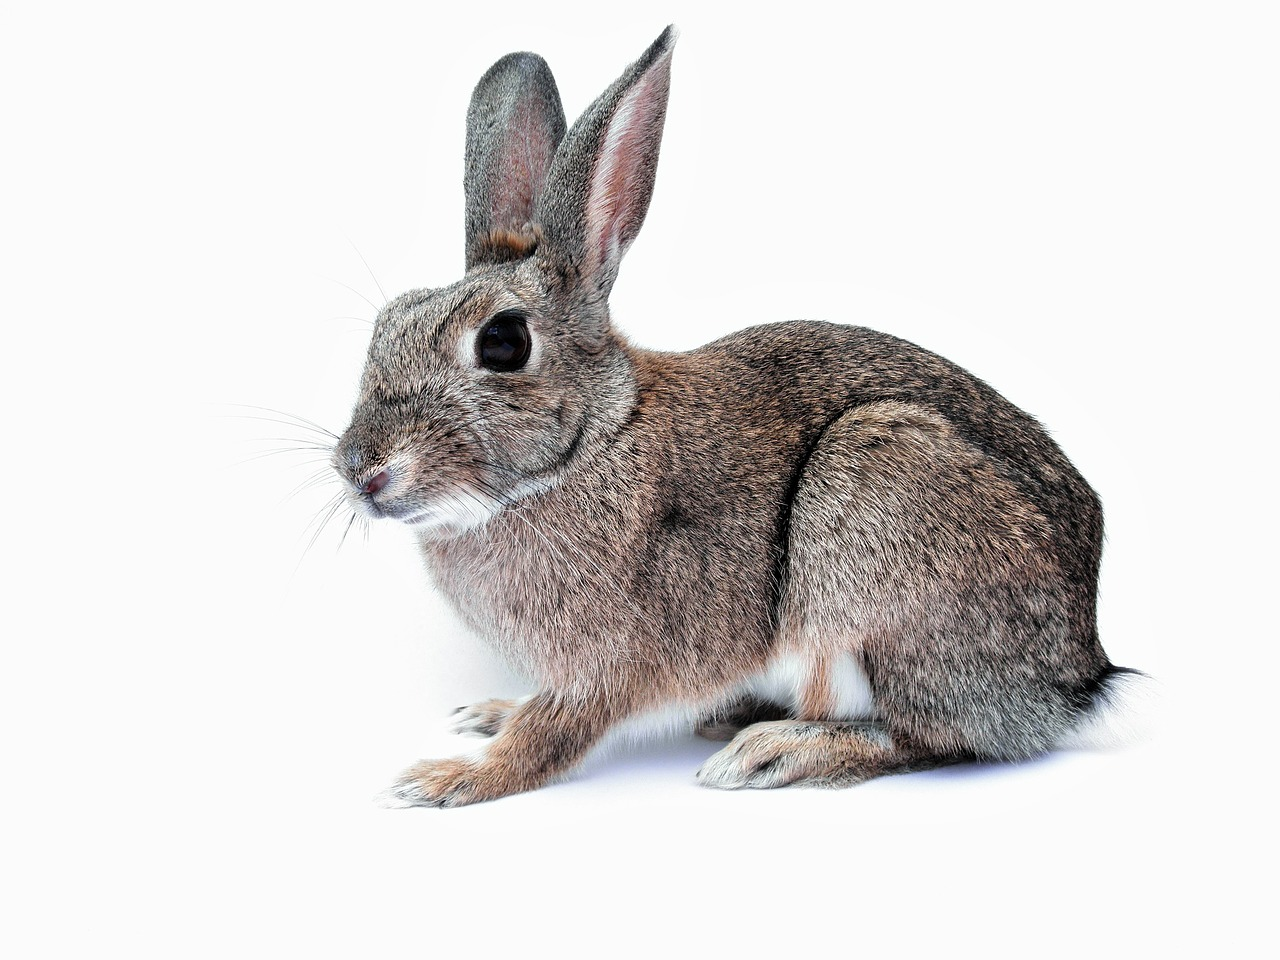
\includegraphics[scale=0.07]{Rabbit1}}
We're told that $r=0.5$, $M=2000$, and $P_0=200$.  Putting it all into the logistic model:
\begin{align*}
P_t &= \dfrac{M}{1+\left(\dfrac{M}{P_0}-1\right)e^{-rt}}\\
P_t &= \dfrac{2000}{1+9e^{-0.5t}}
\end{align*}

Graphing this equation:
\begin{center}
\begin{tikzpicture}
\begin{axis}[
    xmin=0, xmax=12,
    ymin=0, ymax=2000,
    axis lines=center,
    axis on top=true,
    domain=0:1,
    x=0.5cm,
    y=0.002cm,
    xtick={0,1,...,20},
    xticklabels={0,1,...,20},
    ytick={0,200,...,2000},
    yticklabels={0,200,...,2000},
    axis lines=middle,
    axis line style={->},
    x label style={at={(axis description cs:0.5,-0.1)},anchor=north},
    y label style={at={(axis description cs:-0.1,.5)},rotate=90,anchor=south},
    xlabel={Years from Present},
    ylabel={Rabbit Population},
    grid=major
    ]
	\addplot[samples=100,domain=0:12] {2000/(1+9*e^(-0.5*x))};
\end{axis}
\end{tikzpicture}
\end{center}

We can use this model to predict the rabbit population at any point in the future, and we note that according to the model, the rabbit population will level out near the carrying capacity in about 12 years.
\end{example}
\pagebreak

\begin{example}[https://www.youtube.com/watch?v=cd5xQCfLUZM]{Lizard Population}
On an island that can support a population of 1000 lizards, there is currently a population of 600.  These lizards have a lot of offspring and not many natural predators, so they have a very high growth rate of 150\%.  Use a logistic model to predict the lizard population 2 years from now.\\

\marginnote{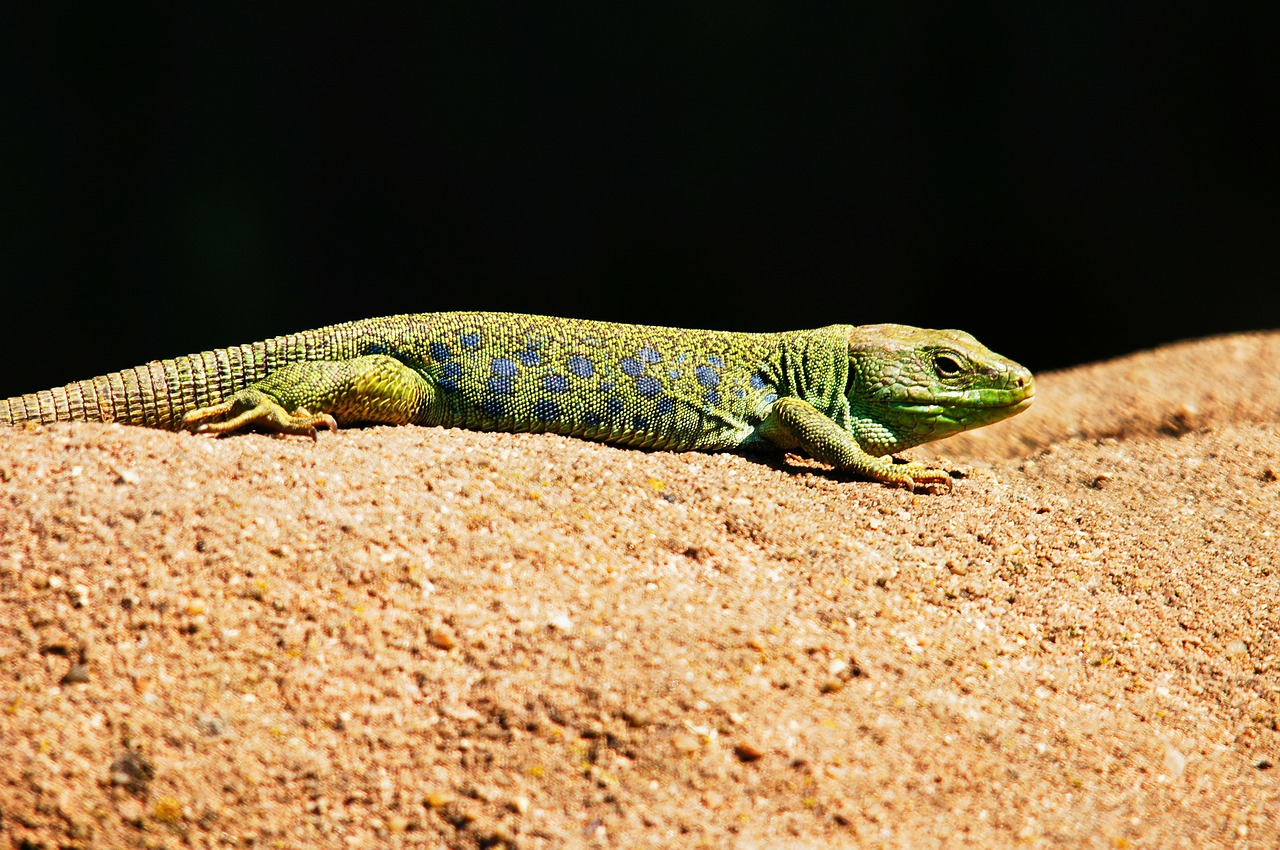
\includegraphics[scale=0.07]{Lizard1}}
Fill in the logistic model:
\begin{align*}
P_t &= \dfrac{M}{1+\left(\dfrac{M}{P_0}-1\right)e^{-rt}}\\
P_t &= \dfrac{1000}{1+\dfrac{2}{3}e^{-1.5t}}
\end{align*}

\begin{center}
\begin{tikzpicture}
\begin{axis}[
    xmin=0, xmax=4,
    ymin=0, ymax=1100,
    axis lines=center,
    axis on top=true,
    domain=0:1,
    x=0.8cm,
    y=0.005cm,
    xtick={0,1,...,20},
    xticklabels={0,1,...,20},
    ytick={0,100,...,1000},
    yticklabels={0,100,...,1000},
    axis lines=middle,
    axis line style={->},
    x label style={at={(axis description cs:0.5,-0.1)},anchor=north},
    y label style={at={(axis description cs:-0.2,.5)},rotate=90,anchor=south},
    xlabel={Years from Present},
    ylabel={Lizard Population},
    grid=major
    ]
	\addplot[samples=100,domain=0:12] {1000/(1+(2/3)*e^(-1.5*x))};
\end{axis}
\end{tikzpicture}
\end{center}

Let $t=2$ to predict the population in 2 years:
\begin{align*}
P_2 &= \dfrac{1000}{1+\dfrac{2}{3}e^{-1.5(2)}}\\
 &= \dfrac{1000}{1+\dfrac{2}{3}\cdot 0.0498}\\
 &= \dfrac{1000}{1.0332}\\
 &\approx 968
\end{align*}
The model predicts that there will be approximately 968 lizards in 2 years.
\end{example}

\begin{try}[http://www.izzomath.com/103text/growthmodels/example3.1/story.html]
A field contains 20 mint plants, and the number of plants increases at a rate of 70\%, but the field can only support a maximum population of 300 plants.  Use the logistic model to predict what the population will be in three years.
\end{try}

\begin{exercises}

\ptwo{One hundred trout are seeded into a lake.  Absent constraint, their population will grow by 70\% a year.  If the lake can sustain a maximum of 2000 trout, use a logistic growth model to estimate the number of trout after 2 years.}
\ptwo{Ten blackberry plants started growing in a yard.  Absent constraint, blackberries will spread by 200\% a month.  If the yard can only sustain 50 plants, use a logistic growth model to estimate the number of plants after 3 months.}

\ptwo{A certain community consists of 1000 people, and one individual has a particularly contagious strain of influenza.  Assuming the community has not had vaccination shots and are all susceptible, the spread of the disease in the community is modeled by \[A = \dfrac{1000}{1+999e^{-0.3t}}\] where $A$ is the number of people who have contracted the flu after $t$ days.
\begin{enumerate}[(a)]
\item How many people have contracted the flu after 10 days?  Round your answer to the nearest whole number.
\item What is the carrying capacity for this model?  Does this make sense?
\item How many days will it take for 750 people to contract the flu?  Round your answer to the nearest whole number.
\end{enumerate}}
\ptwo{A herd of 20 white-tailed deer is introduced to a coastal island where there had been no deer before.  Their population is predicted to increase according to \[A = \dfrac{100}{1+4e^{-0.14t}}\] where $A$ is the number of deer expected in the herd after $t$ years.
\begin{enumerate}[(a)]
\item How many deer will be present after 2 years?  Round your answer to the nearest whole number.
\item What is the carrying capacity for this model?
\item How many years will it take for the herd to grow to 50 deer?  Round your answer to the nearest whole number.
\end{enumerate}}

\end{exercises}


\chapter{Statistics}
\begin{center}\includegraphics[width=\textwidth]{StatChapter}\end{center}

There's a popular joke among statisticians that 64.8\% of all statistics are made up on the spot. How can you tell the difference between good and bad statistics? 
Where do the numbers come from? How is data collected? No other branch of mathematics has a more tremendous impact on our lives than the field of statistics. 
Statistics are everywhere, from crime rates in your city to weight percentiles for children on growth charts. When a research team is testing a new treatment for a disease, they can use statistics to make conclusions based on a relatively small trial and show that there is good evidence that their drug is effective. Statistics allowed prosecutors in the 1950's 
and 60's to demonstrate that racial bias existed in jury panels. In this chapter, you will get a glimpse into this important subject, understanding the essentials and learning to become a wise consumer of statistics. 
\vfill
\pagebreak

\section{Sampling and Graphs}
\setcounter{ExampleCounter}{1}
Let us start with the basics. What is statistics? The field of \textbf{statistics} encompasses collecting, organizing, analyzing and presenting data. \textbf{Data} is simply
collected information. That information can be collected via surveys, polls, records, experiments, studies, or censuses, just to name a few. A \textbf{census} is when we collect data on the entire population, polling each and every individual. As you can imagine, that would take a lot of time and resources. \marginnote{The 2010 census cost about \$13 billion to administer}That is why in the United States, a census occurs only every 10 years. In all other situations, we do what is known as sampling, where we assume that if we study a small portion of the total group, the results will be similar to what we would find if we polled the entire group.

Our goal in statistics, then, is to select a good sample, gather data from the sample, organize and summarize the data, and draw conclusions from the sample about the total population.

\subsection{Population and Sample}

A \textbf{population} is a collection of persons or objects under study. To study the population, we select a \textbf{sample}. The idea of \textbf{sampling} is to select a portion (or subset) of the larger population and study that portion (the sample) to gain information about the population. Sampling is a very practical technique. If you wished to find the average height of students at your school, you probably wouldn't collect data from every single student; this wouldn't be very feasible. It would make more sense to select a sample of students. The data collected would be the students' heights.  In presidential elections, opinion polls sample 1000 to 2000 people. The opinion poll is supposed to represent the views of the people in the entire country. Manufacturers of ice cream take samples to determine if a pint of ice cream actually contains a pint of ice cream.

\begin{example}[https://www.youtube.com/watch?v=-AK3lL3YKOA]{Pet Ownership}
A sample of 2,000 households in the U.S. was selected and asked if they currently own at least one pet. The results show that 69\% of households do own at least one pet.
Identify the sample and population in this situation.\\


\marginnote{\bfseries Solution}
The sample is the 2,000 households and the population is all households in the U.S. Notice that even though the population is not explicitly stated, we can infer it from carefully reading the sentence. 
\end{example}

\begin{try}[http://www.izzomath.com/103text/stats/example1.1/story.html]
A researcher wants to know how citizens of Frederick City felt about a voter initiative. To study this, she goes to the Francis Scott Key Mall in the city, randomly selects 500 shoppers and asks them their opinion. Sixty percent indicate they are supportive of the initiative. What is the sample and population?:
\end{try}

Let's go back and think about finding the average height of students at your school. How would you go about obtaining your sample? Would you sample all your friends, or all your classmates? How about asking people in the library on a Wednesday afternoon? Would any of these sampling techniques give you a good estimate of the average height of all students? 


We have to make sure our sample is not \textbf{biased}, or leaning in a certain direction. Maybe you like to hang out with tall people and all your friends are tall. Maybe only 10 people are in the library on Wednesdays. Your sample must be random and representative in order to get a good estimate of the population data.  A sample is \textbf{random} if everybody in the population has the same chance of being selected into the sample. A sample is \textbf{representative} if it contains the characteristics of the population.

\begin{proc}{Random Samples}
The key to a random sample is that each member of the population is equally likely to be selected.

\paragraph{Examples of Random Samples}
\begin{itemize}
\item If the population is students in a particular classroom, number the students in the classroom from 1 to $n$ and use a random number generator to select numbers between 1 and $n$.
\item If the population is FCC students, list their FCC email accounts and number them, then pick random numbers between 1 and $n$, where $n$ is the number of students.
\end{itemize}

\paragraph{Examples of Biased Samples}
\begin{itemize}
\item \marginnote{Not every resident of the county has a phone, let alone a phone listed in the phone book}If the population is residents of Frederick County, number the entries in the phone book and use a random number generator to select a sample.
\item If the population is American citizens, go to the entrance of Yankee Stadium and poll everyone entering.
\item If the population is FCC students, poll the students in one class.
\end{itemize}

If you're ever unclear on whether or not a sampling method is random, simply ask whether or not every member of the population has an equal chance of being selected.  A random sample gives better results than a biased sample because characteristics that could muddy the results of the study get averaged out by the randomness.
\end{proc}
\vspace{0.5in}

\subsubsection*{Picking Random Numbers with a TI-83}
Your graphing calculator can select random numbers.  To access this menu, press the MATH button and use the left and right arrows to navigate to the PRB tab (PRB for probability).
\begin{center}
\begin{tabular}{l b{0.6\textwidth}}
\includegraphics[width=0.3\textwidth]{RandMenu} & Selecting \texttt{rand} will select a ``random'' (technically pseudo-random, but close enough for us) number between 0 and 1.  Selecting \texttt{randInt(} will allow you to choose a random integer between a given lower and upper bound, or several of those.
\end{tabular}
\end{center}

\begin{center}
\begin{tabular}{l b{0.6\textwidth}}
\includegraphics[width=0.3\textwidth]{RandInt} & To select a single random integer, enter \texttt{randInt(}lower bound\texttt{,}upper bound\texttt{)}, with whatever numbers you want for the lower and upper bounds.  To select $n$ random integers, enter \texttt{randInt(}lower bound\texttt{,}upper bound\texttt{,}$n$\texttt{)}
\end{tabular}
\end{center}
\vfill
\pagebreak

\begin{example}[https://www.youtube.com/watch?v=mm1iQfMgNHE]{Cartwheels}
A coach is interested in how many cartwheels the average college freshman can do at his university. Eight volunteers from the freshman class step forward. After observing their
performance, the coach concludes that college freshmen can do an average of 16 cartwheels in a row without stopping. Is this sample random and representative?\\

\marginnote{\bfseries Solution}
The population is the class of all freshmen at the coach's university. The sample is composed of all freshmen so that is good. However, the sample is poorly chosen because volunteers are more likely to be able to do cartwheels than the average freshman: people who cannot do cartwheels probably did not volunteer! Hence, this sample is not random. We are also not told of the gender of the volunteers. Were they all women, for example? That might affect the outcome (if the school is co-ed). We cannot be sure this sample is representative.

\end{example}

\begin{try}[http://www.izzomath.com/103text/stats/example1.2/story.html]
A substitute teacher wants to know how students in the class did on their last test. The teacher asks the 10 students sitting in the front row to state their latest test score. He concludes from their responses that the class did extremely well. What is the sample and population? Is the sample random and representative? Why or why not?
\end{try}

In general, self-selected samples (or volunteer samples) are not representative of the population.  For this reason, surveys with voluntary responses are not reliable.  People who volunteer their opinion for online reviews, for instance, tend to be strongly positive or negative; the voluntary sample misses everyone in the middle who doesn't have a strong opinion.

The most famous example of this comes from the 1936 presidential election, where the incumbent Democrat, Franklin D. Roosevelt, was challenged by the Republican governor of Kansas, Alf Landon.  The \textit{Literary Digest}, a weekly magazine, boasted that it had correctly predicted the results of the last 4 elections by sending out questionnaires to its huge sample of readers.  In 1936, the \textit{Digest} sent out 10 million questionnaires and received over 2 million responses, predicting that Landon would unseat Roosevelt with a handy victory.  When Election Day came, though, Roosevelt received over 60\% of the popular vote, carrying every state except for Maine and Vermont (including Landon's home state).  It was one of the most lopsided victories in U.S. history.  The reason for the failure of this poll was largely based on the voluntary response nature--those who responded were more likely to be those who were unhappy with the current administration; people who were happy with Roosevelt's programs had no incentive to fill out the questionnaire and send it in.

Largely due to this failure and embarrassment, the \textit{Literary Digest} folded within a few years.  In contrast, a young pollster named George Gallup (whose name is borne by the Gallup polls today) made his name in the 1936 election by correctly predicting the winner with a much smaller, carefully chosen sample.

\subsection{Frequency Distributions}

One of the most fundamental parts of statistics is presenting data clearly. After the data has been collected, it must be presented in a way so that it conveys all the necessary information and is easy for the viewer to understand. It is usually impractical and unhelpful to list all of the data that we gather for our audience; imagine gathering data on standardized test scores in a state and listing thousands of unsorted scores--there would be no way to make sense of the data.  When we present data, we want to show a clear picture of what's going on, without overwhelming our audience with so much data that the reality gets lost in the noise.


The first way that we'll present data is with a \textbf{frequency distribution}, which simply counts how often each data value occurs.  For instance, suppose twenty students were asked how many hours they worked per day. Their responses, in hours, are as follows: \[5, 6, 3, 3, 2, 4, 7, 5, 2, 3, 5, 6, 5, 4, 4, 3, 5, 2, 5, 3.\]
\pagebreak

The table below lists the different data values in ascending order and their frequencies.

\begin{center}
\begin{tabular}{c | c}
\textbf{Data Value} & \textbf{Frequency}\\
\hline
2 & 3\\
3 & 5\\
4 & 3\\
5 & 6\\
6 & 2\\
7 & 1
\end{tabular}
\end{center}

If one data value between 2 and 7 didn't appear in the data set--for example, if none of the students responded that they worked 4 hours per day--we would usually still include the row for 4 and just note that the frequency was 0 for that value.

The \textbf{frequency} is the number of times a data value occurs. According to the table above, there are three students who work two hours, five 
students who work three hours, and so on. The sum of the values in the frequency column, 20, represents the total number of students included in
the sample. 

We can also calculate the \textbf{relative frequency} of each value, which is the ratio of the number of times a value occurs to the total number of outcomes. We can include these in a third column on our frequency table.  To find the relative frequencies, divide each frequency by the total number of students in the sample--in this case, 20. Relative frequencies can be written as fractions, decimals, or as in the table below, as percents.
\begin{center}
\begin{tabular}{c | c | c}
\textbf{Data Value} & \textbf{Frequency} & \textbf{Relative Frequency}\\
\hline
2 & 3 & 3/20 or 15\% \\
3 & 5 & 5/20 or 25\% \\
4 & 3 & 3/20 or 15\% \\
5 & 6 & 6/20 or 30\% \\
6 & 2 & 2/20 or 10\% \\
7 & 1 & 1/20 or 5\%
\end{tabular}
\end{center}
The sum of all the values of the relative frequency column of the table above is 20/20, or 1.  Note, because of rounding, the relative frequency column may not 
always sum to one. However, it should be close to one.


\begin{example}[https://www.youtube.com/watch?v=VQhKtct3nog]{Daily Commute}
Nineteen people were asked how many miles, to the nearest mile, they commute to work each day. They responded as follows: \[2, 5, 7, 3, 2, 10, 18, 15, 20, 7, 10, 18, 5, 12, 13, 12, 4, 5, 10.\] This is summarized in the frequency table below:

\begin{center}
\begin{tabular}{c | c | c}
\textbf{Data Value} & \textbf{Frequency} & \textbf{Relative Frequency}\\
\hline
3 & 3 & 3/19 \\
4 & 1 & 1/19 \\
5 & 3 & 3/19 \\
7 & 2 & 2/19 \\
10 & 3 & 4/19 \\
12 & 2 & 2/19 \\
13 & 1 & 1/19 \\
15 & 1 & 1/19 \\
18 & 1 & 1/19 \\
20 & 1 & 1/19  
\end{tabular}
\end{center}

\begin{itemize}
\item Is the table correct? If it is not correct, what is wrong?\\

It is incorrect, because the frequency column sums to 18, not 19 as it should.  One of the data values was left out.  Besides, two people responded that they commute 2 miles, and that doesn't appear on the table at all.\\

\item True or false: Three of the people surveyed commute three miles. If the statement is not correct, what should it be? If the table is incorrect, make the corrections.\\

False.  The frequency for 3 miles should be 1.  When building the table, the two that responded 2 miles got lumped into the 3 category.\\

\item What fraction of the people surveyed commute five or seven miles?\\

5/19\\

\item What fraction of the people surveyed commute 12 miles or more? Less than 12 miles? Between 5 and 13 miles (not including those who commute exactly 5 or exactly 13 miles)?\\

7/19, 12/19, 7/19
\end{itemize}
\end{example}

Sometimes, it's more practical to make a \textbf{grouped frequency distribution}, where the frequencies are not single numbers, but groups of numbers.

For instance, suppose you gathered data on how long it took you to get ready in the morning.  For 40 days, you measured the amount of time between when your alarm went off and you left the house, and you got the following results in minutes:
\begin{center}
\begin{tabular}{c c c c c c c c c c}
35.6 & 28.7 & 25.5 & 23.2 & 23.7 & 32.1 & 29.6 & 19.5 & 21.4 & 13.6\\
24.9 & 26.7 & 25.8 & 31.8 & 30.4 & 20.1 & 25.3 & 29.9 & 37.5 & 26.6\\
32.3 & 36.5 & 18.5 & 17.7 & 15.2 & 24.7 & 21.4 & 16.6 & 19.5 & 30.3\\
38.7 & 27.4 & 22.9 & 24.6 & 28.5 & 17.5 & 31.4 & 32.2 & 21.6 & 28.4\\
\end{tabular}
\end{center}

If we built a frequency distribution with one row for each distinct value, the table would not give any useful information; it wouldn't serve the purpose of a frequency distribution, which is to give a preliminary idea of where the data is clustered and where it is spread out.

Instead, we can make a grouped frequency distribution by grouping together data values in the same range.  If we do this for the data set above by grouping in sets of 5, we get the grouped frequency distribution below.
\begin{center}
\begin{tabular}{c | c}
\textbf{Data Values} & \textbf{Frequency}\\
\hline
10--less than 15 & 1\\
15--less than 20 & 7\\
20--less than 25 & 10\\
25--less than 30 & 11\\
30--less than 35 & 7\\
35--less than 40 & 4\\
\end{tabular}
\end{center}

This distribution has six categories, called \textbf{classes}.  The starting values of the classes (10, 15, 20, etc.) are called the \textbf{lower class limits}, and the ending values are called the \textbf{upper class limits}.  The \textbf{class width} is the difference between the lower class limits.  Notice that if we subtract $20-15$, we get 5.  Therefore, the class width in this example is 5.

\begin{proc}{Choosing Classes}
When building a grouped frequency distribution, you'll usually have the freedom to choose how you want to separate the classes.  Here are some guidelines you should follow:
\begin{itemize}
\item Each class should be the same width.  Notice in the example above that each class was five units wide.  If not, the grouped frequency distribution would not give a clear picture of how the data is arranged.
\item Classes cannot overlap.  In the example above, we avoided overlap by letting the first class go up to ``less than 15'' and having the second class start at 15, and similarly for the other classes.  If the classes overlapped at 15, it wouldn't be clear into which category we should place a data value of 15.0.
\item Avoid empty classes if possible.  This can occur if you choose to have too many classes.
\item Don't make open-ended classes.  For instance, in the example above we didn't make the last class ``35 and above,'' which would have been an open-ended class.  The reason not to do this is that it violates the first guideline about having all classes have the same width.
\end{itemize}
\end{proc}

To find the appropriate class width to use, you can start by deciding on the number of classes you want to use. In our example above, we chose 6. Then the class width is found by dividing the distance from the minimum to the maximum by the number of classes. 

\begin{formula}{Class Width}

\[\textrm{Class Width } = \dfrac{\textrm{Maximum - Minimum}}{\textrm{Number of Classes}}\]
Round UP to the next whole number.
\end{formula}

\subsection{Histograms}

Let's revisit the example we looked at earlier of the twenty students and the number of hours worked each day.
\begin{center}
\begin{tabular}{c | c}
\textbf{Data Value} & \textbf{Frequency}\\
\hline
2 & 3\\
3 & 5\\
4 & 3\\
5 & 6\\
6 & 2\\
7 & 1
\end{tabular}
\end{center}

We can represent a frequency distribution with a picture instead of a list of numbers, which is helpful to our visual-oriented brains.  The graph we build from a frequency distribution is called a \textbf{histogram}.  A histogram is a bar graph\marginnote{Note carefully: a \textbf{bar graph} has gaps between the bars.  A \textbf{histogram} (what we do in this chapter) has no gaps.} with a bar for each class in the frequency distribution, and the height of the bar represents the frequency listed for that class.

The vertical axis is labeled either frequency or relative frequency, the horizontal axis is labeled with what the data represents (for instance, hours worked per day). The histogram from the working hours frequency distribution is below: 

\begin{center}
\includegraphics[scale=0.6]{HoursWorkedHistogram}
\end{center}

\begin{proc}{Using Your Calculator}
The TI calculator will construct a histogram for you.  You have two options: entering the frequency distribution into the calculator, or entering the raw data and letting the calculator find the frequency of each value.

\paragraph{Option 1:} Enter the frequency distribution
\begin{enumerate}
\item Press the \textbf{STAT} button to enter the statistics menu
\item Choose the \textbf{Edit} option to edit the data list
\item Enter the classes (or values if it isn't a grouped table) into L1 and enter the frequency into L2
\item Choose the \textbf{STATPLOT} option by clicking the \textbf{2nd} and \textbf{Y=} buttons
\item Turn Plot1 On and choose the histogram option, with the data (Xlist) in L1 and the frequency in L2
\item Press \textbf{ZOOM} and choose the "ZoomStat" option
\end{enumerate}
By pressing the \textbf{TRACE} button, you can see the frequency of the bars.\\

\includegraphics[height=1.25in]{Calc1}
\includegraphics[height=1.25in]{Calc2}
\includegraphics[height=1.25in]{Calc3}
\includegraphics[height=1.25in]{Calc4}

\paragraph{Option 2:} Enter the raw data\\

Instead of using L1 and L2, simply enter the data into L1 and enter ``1'' for the Freq option when creating the histogram.  You can change the width of the classes by changing Xscl under the \textbf{WINDOW} menu.
\begin{center}
\includegraphics[height=1in]{Calc2b}
\includegraphics[height=1in]{Calc3b}
\includegraphics[height=1in]{Calc4b}
\end{center}
\end{proc}
\vspace{0.5in}

The graph below was created by the TI-83 using the data about getting ready in the morning, by entering the raw data in L1:
\begin{center}
\includegraphics[scale=1]{Calc5}
\end{center}
\vfill
\pagebreak

\subsection{Stem-and-Leaf Plots}
There is one major downside to grouped frequency distributions: some of the data gets lost in the summary.  In other words, maybe in an example all we know is that there are 10 observations between 20 and 25, but we don't know exactly what all those observations are.  This is an example of the trade-off between clarity and precision: often, the more precise we are, the less clear our summary will be.

To split the difference and display the data in a way that exhibits where it is clustered without losing any information about the data is to use a \textbf{stem-and-leaf} plot.  Here, the data is grouped by tens; each tens value is a stem, and all the data points that have that tens value are listed as the leaves.  We'll illustrate with an example, using the same data set we used to construct the grouped frequency distribution above, but this time without the decimal places:
\begin{center}
\begin{tabular}{c c c c c c c c c c}
35 & 28 & 25 & 23 & 23 & 32 & 29 & 19 & 21 & 13\\
24 & 26 & 25 & 31 & 30 & 20 & 25 & 29 & 37 & 26\\
32 & 36 & 18 & 17 & 15 & 24 & 21 & 16 & 19 & 30\\
38 & 27 & 22 & 24 & 28 & 17 & 31 & 32 & 21 & 28\\
\end{tabular}
\end{center}

The tens places are 1, 2, and 3, and each of them gets a category:
\begin{center}
\begin{tabular}{r | l}
Stems & Leaves\\
\hline
1 & {\color{white}3 5 6 7 7 8 9 9}\\
2 & {\color{white}0 1 1 1 2 3 3 4 4 4 5 5 5 6 6 7 8 8 8 9 9}\\
3 & {\color{white}0 0 1 1 2 2 2 5 6 7 8}
\end{tabular}
\end{center}

Finally we go through (carefully) and find each value that begins with a 1 and list the ones place of each of them under the first category, and similarly with the other two categories.
\begin{center}
\begin{tabular}{r | l}
Stems & Leaves\\
\hline
1 & 3 5 6 7 7 8 9 9\\
2 & 0 1 1 1 2 3 3 4 4 4 5 5 5 6 6 7 8 8 8 9 9\\
3 & 0 0 1 1 2 2 2 5 6 7 8
\end{tabular}
\end{center}

Notice that we arranged the leaves in order; this isn't strictly necessary, but it makes the data a bit more orderly.

Once again, this stem-and-leaf plot illustrates where the data is clustered, as the length of each row of leaves is equivalent to the height of a bar on a histogram, but it does this without losing any information.  In other words, if we were simply given the stem-and-leaf plot, we could completely recreate the data set.\\

For three-digit data values (or longer), the leaves are usually still the last digits (the unit digits), and the stems are everything before that.  For instance, observe the data set below and the corresponding stem-and-leaf plot.

\begin{center}
\begin{tabular}{c c c c c c c c c c}
135 & 128 & 125 & 123 & 123 & 132 & 129 & 119 & 121 & 113\\
124 & 126 & 125 & 131 & 130 & 120 & 125 & 129 & 137 & 126\\
\end{tabular}
\end{center}

\begin{center}
\begin{tabular}{r | l}
Stems & Leaves\\
\hline
11 & 3 9\\
12 & 0 1 3 3 4 5 5 5 6 6 8 9 9\\
13 & 0 1 2 5 7
\end{tabular}
\end{center}






\begin{exercises}

\textit{For problems 1--2, identify the population and sample.}\\
\ptwo{A political scientist surveys 28 of the current 106 representatives in a state's congress. Of them, 14 said they were supporting a new education bill, 12 said they were not supporting the bill, and 2 were undecided.}
\ptwo{The city of Frederick has 9500 registered voters. There are two candidates for the city council in an upcoming election: Marfani and Rahman. The day before the election, a telephone poll of 350 randomly selected registered voters was conducted. Of them, 112 said they would vote for Marfani, 207 said they would vote for Rahman, and 31 were undecided.}\\ 

\textit{For exercises 3--6, identify the most relevant source of bias in the situation.}\\
\ptwo{To determine opinions on voter support for a downtown renovation project, a surveyor randomly questions people working in downtown businesses.}
\ptwo{To select a sample, a pollster calls every 100th name in the phone book.}

\ptwo{Suppose pollsters call people at random, but once they have met their quota of 390 Democrats, they only gather people who do not identify themselves as a Democrat.}
\ptwo{A survey seeks to investigate whether a new pain medication is safe to market to the public. They test by randomly selecting 300 men from a set of volunteers.}

\pone{Fifty part-time students were asked how many courses they were taking this semester. The (incomplete) results are shown below. Fill in the blank cells to complete the table.
\begin{center}
\begin{tabular}{c | c | c }
\textbf{\# of courses} & \textbf{Frequency} & \textbf{Relative Frequency}\\
\hline
1 & 30 & 0.6\\
2 & 15 &    \\
3 &    &    
\end{tabular}
\end{center}
}

\ptwo{The following is the average daily temperature for Frederick, Maryland for the month of June: \begin{align*}74, 60, 58, 58, 64, 67, 64, 74, 72, 70,\\ 78, 80, 80, 79, 80, 80, 70, 83, 76, 78,\\ 81, 78, 81, 70, 70, 71, 66, 66, 68, 74.\end{align*}
\begin{enumerate}[(a)]
\item Construct a grouped frequency and relative frequency distribution using a class width of 5.
\item Construct a histogram from the frequency distribution. 
\end{enumerate}
}
\ptwo{A researcher gathered data on hours of video games played by school-aged children and young adults. She collected the following data: \begin{align*}0, 0, 1, 1, 1, 2, 2, 3, 3, 3,\\ 4, 4, 4, 4, 5, 5, 5, 6, 6, 7,\\ 7, 7, 8, 8, 8, 8, 8, 9, 9, 9,\\ 10, 10, 11, 12, 12, 12, 12, 13. \end{align*}
\begin{enumerate}[(a)]
\item Construct a grouped frequency and relative frequency distribution using 6 classes.
\item Construct a histogram from the frequency distribution. 
\end{enumerate}
}

\pone{
The following stem-and-leaf plots compare the ages of 30 actors and 30 actresses at the time they won the Oscar award for Best Actor or Actress.
\begin{center}
\begin{tabular}{|r | c | l|}
\hline
Actors & Stems & Actresses\\
\hline
& 2 & 146667\\
\hline
98753221 & 3 & 00113344455778\\
\hline
88776543322100 & 4 & 11129\\
\hline
6651 & 5 & \\
\hline
210 & 6 & 011\\
\hline
6 & 7 & 4\\
\hline
& 8 & 0\\
\hline
\end{tabular}
\end{center}
\begin{enumerate}[(a)]
\item What is the age of the youngest actor to win an Oscar?
\item What is the age difference between the oldest and the youngest actress to win an Oscar?
\item What is the oldest age shared by two actors to win an Oscar?
\end{enumerate}
}

\textit{For exercises 11--14, use the frequency table below, which contains the total number of deaths worldwide as a result of earthquakes for the period from 2000 to 2012.}\\
\begin{center}
\begin{tabular}{c | r}
\textbf{Year} & \textbf{Total Number of Deaths}\\
\hline
2000 & 231\\
2001 & 21,357\\
2002 & 11,685\\
2003 & 33,819\\
2004 & 228,802\\
2005 & 88,003\\
2006 & 6,605\\
2007 & 712\\
2008 & 88,011\\
2009 & 1,790\\
2010 & 320,120\\
2011 & 21,953\\
2012 & 768\\
\textbf{Total} & \textbf{823,356}
\end{tabular}
\end{center}

\ptwo{What is the frequency of deaths measured from 2006 through 2009?}
\ptwo{What percentage of deaths occurred after 2009 (from 2010 onwards)?}

\ptwo{What is the relative frequency of deaths that occurred in 2003 or earlier?}
\ptwo{What is the percentage of deaths that occurred in 2004?}


%\textit{For problems 14--17, use the frequency table below which shows the percentage of smokers in different education categories. Data is from the CDC.}\\
%\begin{center}
%\begin{tabular}{l | c}
%\textbf{Education} & \textbf{Percentage Who Smoke}\\
%\hline
%0--12 (no diploma) & 26\% \\
%GED Diploma & 43\% \\
%High school Graduate & 25\%\\
%Some college & 23\%\\
%Associate degree & 21\%\\
%Bachelor degree & 12\%\\
%Graduate degree & 7\%
%\end{tabular}
%\end{center}

%\ptwo{What percentage of smokers have at least a diploma?}
%\ptwo{What percentage of smokers have college experience, but no college diploma?}

%\ptwo{What is the relative frequency for those with college degrees (including associate, bachelor, and graduate degrees)?}
%\ptwo{What is the percentage who smoke with Associate degrees?}

\pone{What is wrong with the following grouped frequency distribution?
\begin{center}
\begin{tabular}{c | c}
\textbf{Grades} & \textbf{Frequency}\\
\hline
50--55 & 2\\
55--60 & 4\\
60--70 & 9\\
70--80 & 15\\
80--90 & 7\\
90 and above & 4
\end{tabular}
\end{center}
\begin{enumerate}[(a)]
\item The classes do not all have the same width.
\item The classes overlap.
\item There are open-ended classes.
\item All of the above.
\end{enumerate}

}



\end{exercises}

\section{Measures of Center}
\setcounter{ExampleCounter}{1}
What comes to mind when you think of the word ``average?'' You may think of situations where the average is used: average income, average height, average number of Facebook friends, average test score, etc. The average is a type of center. It tells us the middle of the data. We call the average a \textbf{measure of center}, because it gives a quick snapshot of what a \textit{typical} data point is. But the average is not the only measure of center. In this section, we'll examine several measures of center, how to calculate them and when best to use them.

\subsection{The Mean}
The \textbf{mean} is what most people call the average. To find the mean, you add all the values and divide by the number of values. We can write this in mathematical notation. The Greek letter sigma $\Sigma$ is the symbol for sum. When you see $\Sigma x$, that stands for ``the sum of x.'' The symbol for the mean is $\overline{x}$, read ``x bar.'' Using this information, we can devise a formula for the mean.

\begin{formula}{Mean}
The mean of a sample of size $n$ is
\[\overline{x} = \dfrac{\sum x}{n}.\]

The mean of a population of size $N$ is
\[\mu = \dfrac{\sum x}{N}.\]
\end{formula}

We must note that the symbol for the sample mean is $\overline{x}$, whereas the symbol for population mean is $\mu$ (the lowercase Greek letter, read ``mu'' and pronounced ``mew''). You can assume that the data sets given throughout this section are all samples; hence the mean will be $\overline{x}$.

\begin{example}[https://www.youtube.com/watch?v=CDkM8Hojqg0]{AIDS Patients}
AIDS data indicating the number of months a patient with AIDS lives after taking a new antibody drug are as follows (smallest to largest):
\begin{center}
\begin{tabular}{c c c c c c c c c c}
3 & 4 & 8 & 8 & 10 & 11 & 12 & 13 & 14 & 15\\
15 & 16 & 16 & 17 & 17 & 18 & 21 & 22 & 22 & 24\\
24 & 25 & 26 & 26 & 27 & 27 & 29 & 29 & 31 & 32\\
33 & 33 & 34 & 34 & 35 & 37 & 40 & 44 & 44 & 47\\
\end{tabular}
\end{center}
Calculate the mean.\\

\marginnote{\bfseries Solution}
The calculation for the mean is \[\overline{x} = \frac{3 + 4 + 8 + 8 + 10 + 11 + 12 +...+ 40 + 44 + 44 + 47}{40} = 23.575 \textrm{ months.}\]
To take into account repeated values, we can rewrite the formula. Since the value 8 is repeated twice, instead of using 8+8, we can write (2)(8), and similarly for other repeated values. Hence, we would get\marginnote{Notice that the answer in this alternate solution is rounded to one decimal place.}:\
\[\overline{x} = \frac{3 + 4 + (2)(8) + 10 + ... + 40 + (2)(44) + 47}{40} \approx 23.6 \textrm{ months.}\]
\end{example}
\vfill
\pagebreak

\begin{proc}{Using Your Calculator}
The TI calculator can find the mean for you.
\begin{enumerate}
\item To enter data into the list editor, press \textbf{STAT} then choose option 1:Edit, then enter the data values into list L1.
\item Press \textbf{STAT} and use the arrow button to navigate to the right to the CALC menu. 
\item Choose option 1:1-VarStats. Press the \textbf{2ND} button, then \textbf{1} for list L1. Press \textbf{ENTER}.
\end{enumerate}

\includegraphics[height=1.5in]{Calc1Sec1_2}
\includegraphics[height=1.5in]{Calc2Sec1_2}
\includegraphics[height=1.5in]{Calc3Sec1_2}
\includegraphics[height=1.5in]{Calc4Sec1_2}
\end{proc}

\begin{try}[http://www.izzomath.com/103text/stats/example2.1/story.html]
The following data show the number of months patients typically wait on a transplant list before getting surgery. Calculate the mean using your calculator.
\begin{center}
\begin{tabular}{c c c c c c c c c c}
3 & 4 & 5 & 7 & 7 & 7 & 7 & 8 & 8 & 9\\
9 & 10 & 10 & 10 & 10 & 11 & 12 & 12 & 12 & 13\\
14 & 14 & 15 & 15 & 17 & 17 & 18 & 19 & 19 & 19\\
21 & 21 & 22 & 22 & 23 & 24 & 24 & 24 & 24
\end{tabular}
\end{center}
\end{try}

The mean can also be calculated from a frequency distribution (as long as it is not grouped).  To illustrate this, consider the following frequency distribution of the data in the example from the previous section about how many hours students worked:
\begin{center}
\begin{tabular}{c | c}
\textbf{Data Value} & \textbf{Frequency}\\
\hline
2 & 3\\
3 & 5\\
4 & 3\\
5 & 6\\
6 & 2\\
7 & 1
\end{tabular}
\end{center}

Recall that this means that there are three 2's, five 3's, and so on.  To calculate the mean, we need to add them all up, but we can do this by multiplying each value by how often it occurs and adding up those results (note that this is exactly what we did at the end of the example about AIDS patients).

\[\overline{x} = \dfrac{2(3)+3(5)+4(3)+5(6)+6(2)+7(1)}{20} = 4.1\]
\vfill
\pagebreak

\subsection{The Median}
We noted at the beginning of this section that we have several measures of center, or ways to describe what a typical data point is.  Why is this necessary?  Since the mean is easy to calculate, why don't we always just use that?

To illustrate why, let's look at the following data set, which shows the income for a sample of 5 people: 
\begin{center}
\begin{tabular}{c c c c c}
\$30,000 & \$45,000 & \$50,000 & \$52,000 & \$1,000,000
\end{tabular}
\end{center}

Calculating the mean for this data set yields \$235,400. Does the mean give a true picture for the center of the data? Can I rightfully say the average person in my data set earns roughly \$235,000? Obviously, the answer is no, since 80\%--or 4/5--of the people in this group earn less than \$53,000. When we have an \textbf{outlier}--a number far removed from the majority of data values--in our data, we should use the median instead of the mean to give a measure of center.

The \textbf{median} is the middle value of a data set when the data is ordered. It is denoted with a capital letter $M$. To find the median, sort the data in order from smallest to largest. If there are an odd number of values in the data set, then the median is the middle value. If there are an even number of values in the data set, then the median is the average or mean of the two middle values.

\begin{example}[https://www.youtube.com/watch?v=KNEKKx8GYHg]{AIDS Patients}
Let's return to our AIDS data set. The data has already been arranged in order from smallest to largest:\begin{center}
\begin{tabular}{c c c c c c c c c c}
3 & 4 & 8 & 8 & 10 & 11 & 12 & 13 & 14 & 15\\
15 & 16 & 16 & 17 & 17 & 18 & 21 & 22 & 22 & 24\\
24 & 25 & 26 & 26 & 27 & 27 & 29 & 29 & 31 & 32\\
33 & 33 & 34 & 34 & 35 & 37 & 40 & 44 & 44 & 47\\
\end{tabular}
\end{center}
Let's find the median.\\

\marginnote{\bfseries Solution}
Since there are an even number of values, we have to take the average of the two middle values. Because there are 40 values, the two middle values are the 20th and 21st values.\begin{center}
\begin{tabular}{c c c c c c c c c c}
3 & 4 & 8 & 8 & 10 & 11 & 12 & 13 & 14 & 15\\
15 & 16 & 16 & 17 & 17 & 18 & 21 & 22 & 22 & {\Large\bfseries 24}\\
{\Large\bfseries 24} & 25 & 26 & 26 & 27 & 27 & 29 & 29 & 31 & 32\\
33 & 33 & 34 & 34 & 35 & 37 & 40 & 44 & 44 & 47\\
\end{tabular}
\end{center}
Here, the 20th and 21st values are both 24. The average of 24 and 24 is 24. So the median is \[M = \textrm{ 24 months.}\]
\end{example}

Note that, like the mean, the units of the median are the same as the original data values.

You can also use the TI Calculator to find the median. The steps are the same as to find the mean; just use the arrow keys to scroll down to the median.
\vfill
\pagebreak

\begin{proc}{Where's the Median?}
To find the median, we want to be able to quickly figure out what position to count to in the ordered data set.  To do this, calculate \[\dfrac{n+1}{2},\] where $n$ is the size of the data set.  Notice that this is the average of 1 and $n$, so it makes sense that this would be halfway between them.
\begin{itemize}
\item If $n$ is odd, $\dfrac{n+1}{2}$ is a whole number.  Count to that position and there you'll find the median.
\item If $n$ is even, $\dfrac{n+1}{2}$ is halfway between two whole numbers.  Find the average of the values at those two positions.
\end{itemize}

For instance, in the example above, $n$ was 40, so we calculated $\dfrac{n+1}{2} = 20.5$, so we knew that the median would be between positions 20 and 21 (the average of the numbers in those positions).
\end{proc}

\begin{try}[http://www.izzomath.com/103text/stats/example2.2/story.html]
The following data shows the number of months patients typically wait on a transplant list before getting surgery. Calculate the median either by hand or using your calculator.
\begin{center}
\begin{tabular}{c c c c c c c c c c}
3 & 4 & 5 & 7 & 7 & 7 & 7 & 8 & 8 & 9\\
9 & 10 & 10 & 10 & 10 & 11 & 12 & 12 & 12 & 13\\
14 & 14 & 15 & 15 & 17 & 17 & 18 & 19 & 19 & 19\\
21 & 21 & 22 & 22 & 23 & 24 & 24 & 24 & 24
\end{tabular}
\end{center}
\end{try}

Just like we did with the mean, we can calculate the median from a frequency distribution.  Let's use the same frequency distribution we did before.
\begin{center}
\begin{tabular}{c | c}
\textbf{Data Value} & \textbf{Frequency}\\
\hline
2 & 3\\
3 & 5\\
4 & 3\\
5 & 6\\
6 & 2\\
7 & 1
\end{tabular}
\end{center}

To find the median, we calculate what position it will occupy in the data set.  Since there are 20 data points, $\dfrac{n+1}{2}=10.5$, so the median will be between the 10th and 11th positions.

If we count through the ordered data set, we go through three 2's, five 3's, and then three 4's, which brings us to the 11th position.  The 10th and 11th positions are both occupied by 4's, so $M=4$.

\paragraph{Outliers:} Let's revisit our income data set:
\begin{center}
\begin{tabular}{c c c c c}
\$30,000 & \$45,000 & \$50,000 & \$52,000 & \$1,000,000
\end{tabular}
\end{center}

The median is \$50,000, which is a more accurate measure of center than the mean. This shows the mean is \textit{sensitive} to outliers, whereas the median is \textit{resistant} to outliers. 

\begin{proc}{Mean and Median}
When outliers are present, the median is a better measure of center. When outliers are absent, the mean can be used.
\end{proc}
\pagebreak

\begin{example}[https://www.youtube.com/watch?v=9H2H_DixDQs]{Siblings} 
A dozen people were asked how many siblings they have. The data is as follows: 
\begin{center}
\begin{tabular}{c c c c c c c c c c c c}
0 & 0 & 1 & 1 & 2 & 2 & 4 & 4 & 5 & 5 & 6 & 6
\end{tabular}
\end{center}
Find the mean and median. Then write a sentence or two explaining why the data values result in those particular mean and median.\\

\marginnote{\bfseries Solution}
The mean is $\overline{x} = 3$ siblings and the median is also $M$ = 3 siblings. This is because there are an equal number of high and low values and they are evenly spaced out.
\end{example}

The sibling data above is called \textbf{symmetric}. Symmetric data is balanced around the mean. A data set is symmetric if the mean and median are roughly equal.

\begin{example}[https://www.youtube.com/watch?v=INc8CRq3JfA]{Salaries}
Suppose that in a small town of 50 people, one person earns \$5,000,000 per year and the other 49 each earn \$30,000. Which is the better measure of the ``center'': the mean or the median?\\

\marginnote{\bfseries Solution}
Since an outlier (\$5,000,000) is present, the median would be a better measure of center.  This is why you'll often find the median salary in a region reported rather than the mean.
\end{example}

When trying to decide whether to use the mean or the median as the measure of the center of a data set, compare them to decide if they are drastically different.  Of course, the best policy is to report both of them and compare them to determine whether the data set is symmetric or \textit{skewed}.

\subsection{The Mode}

There is another, less used, measure of center: the mode. The \textbf{mode} is the most frequently occurring value. There can be more than one mode in a data set as long as those values have the same frequency and the frequency is the highest. A data set with two modes is called \textbf{bimodal}.

\begin{example}[https://www.youtube.com/watch?v=shIDfeUatMU]{Exam Scores}
Statistics exam scores for 20 students are as follows:
\begin{center}
\begin{tabular}{c c c c c c c c c c}
50 & 53 & 59 & 59 & 63 & 63 & 72 & 72 & 72 & 72\\
72 & 76 & 78 & 81 & 83 & 84 & 84 & 84 & 90 & 93
\end{tabular}
\end{center}
Find the mode.\\

\marginnote{\bfseries Solution}
The most frequent score is 72, which occurs five times. \begin{center}Mode = 72.\end{center}
\end{example}

\begin{try}[http://www.izzomath.com/103text/stats/example2.5/story.html]
The number of books checked out from the library from 25 students are as follows: 
\begin{center}
\begin{tabular}{c c c c c c c c c c}
0 & 0 & 0 & 1 & 2 & 3 & 3 & 4 & 4 & 5\\
5 & 7 & 7 & 7 & 7 & 8 & 8 & 8 & 8 & 9\\
10 & 10 & 11 & 11 & 12 & & & & &
\end{tabular}
\end{center}
Find the mode.
\end{try}

The mode can also be observed by looking at a frequency distribution (look for the category with the highest frequency) or a histogram (look for the tallest bar).

\begin{exercises}

\ptwo{Which is the greatest of the following data set: the mean, median or mode?
\[11, 11, 12, 12, 12, 12, 13, 15, 17, 22, 22, 22\]}
\ptwo{Which is the greatest of the following data set: the mean, median or mode?
\[80, 83, 83, 87, 87, 87, 91, 97, 98\]}

\ptwo{One hundred teachers attended a seminar on mathematical problem solving. The attitudes of a representative sample of 12 of the teachers were measured before and after the seminar. The 12 change scores are as follows:
\[3, 8, -1, 2, 0, 5, -3, 1, -1, 6, 5, -2\]
\begin{enumerate}[(a)]
\item What is the mean change score?
\item What is the median change score?
\item What is the best measure of center for this data set: the mean or the median? Why?
\end{enumerate}
}
\ptwo{The following are the amounts of total fat (in grams) in different kinds of sweet treats available at your local donut shop:
\begin{align*}16, 17, 16, 13, 15, 17, 16, 14, 15, 17,\\ 18, 18, 16, 16, 15, 20, 22, 19, 25, 15, 15.\end{align*}
\begin{enumerate}[(a)]
\item What is the mean amount of fat?
\item What is the median amount of fat?
\item What is the best measure of center for this data set: the mean or the median? Why?
\end{enumerate}
}

\ptwo{In a neighborhood donut shop, one type of donut has 530 calories, three types of donuts have 330 calories, four types of donuts have 320 calories, seven types of donuts have 410 calories, and five types of donuts have 380 calories. Find the mean and median calories of the donuts.} 
\ptwo{In a recent issue of \textit{IEEE Spectrum}, 84 engineering conferences were announced. Four conferences lasted 2 days, 36 lasted 3 days, 18 lasted 4 days, 19 lasted 5 days, 4 lasted 6 days, 1 lasted 7 days, 1 lasted 8 days, and 1 lasted 9 days. Find the mean and median length (in days) of an engineering conference.}

\ptwo{A researcher gathered data on hours of video games played by school-aged children and young adults. She collected the following data: \begin{align*}0, 0, 1, 1, 1, 2, 2, 3, 3, 3,\\ 4, 4, 4, 4, 5, 5, 5, 6, 6, 7,\\ 7, 7, 8, 8, 8, 8, 8, 9, 9, 9,\\ 10, 10, 11, 12, 12, 12, 12, 13.\end{align*}
Find the mean and median number of hours.}
\ptwo{The following are the sizes in square feet of the seventeen new faculty offices in the mathematics department at Frederick Community College: \begin{align*}202, 120, 120, 120, 137, 167, 122, 111, 109,\\ 108, 102, 108, 103, 103, 103, 106, 127.\end{align*}
Find the mean and median square footage.}\\

\textit{In exercises 9--10, find the mean, median, and mode for each data set. If there is no mode, state so.}

\ptwo{83, 83, 87, 80, 91, 87, 97, 98}
\ptwo{1, 1, 2, 2, 2, 2, 3, 3, 3, 4, 5, 5, 5, 5}\\

\textit{In exercises 11--14, find the mean and median. Then write a sentence or two explaining why the data values result in those particular means and medians.}

\ptwo{0, 0, 1, 1, 2, 2, 6, 6, 7, 7, 8, 8}
\ptwo{0, 0, 1, 1, 2, 2, 6, 7, 8}

\ptwo{0, 0, 1, 1, 8}
\ptwo{1, 1, 1, 1, 1, 1, 8}

\ptwo{Fifteen students took a statistics pre-test and post-test. The results are below. Find the mean and median pre-test and post-test scores. Then write a sentence or two about what the mean and median tell you in this case. A score of 28 is considered a perfect score.
\begin{center}
\begin{tabular}{c | c | c}
\textbf{Student} & \textbf{Pre-test} & \textbf{Post-test}\\
\hline
& & \\
1 & 9 & 22 \\
2 & 11 & 28 \\
3 & 9 & 18 \\
4 & 4 & 24 \\
5 & 10 & 25 \\
6 & 11 & 16 \\
7 & 9 & 19 \\
8 & 9 & 20 \\
9 & 7 & 18 \\
10 & 8 & 14 \\
11 & 5 & 16 \\
12 & 15 & 26 \\
13 & 12 & 21 \\
14 & 0 & 14 \\
15 & 9 & 13
\end{tabular}
\end{center}
}
\ptwo{Below are the ages and salaries (in thousands of dollars) for CEOs of small companies. Find the mean and median age and salary. Then write a sentence or two about what the mean and median tell you. Data from: http://lib.stat.cmu.edu/DASL/Datafiles/ceodat.html.
\begin{center}
\begin{tabular}{c | c | c}
\textbf{CEO} & \textbf{Age} & \textbf{Salary}\\
\hline
& & \\
1 & 53 & 145 \\
2 & 43 & 621 \\
3 & 33 & 262 \\
4 & 45 & 208 \\
5 & 46 & 362 \\
6 & 55 & 424 \\
7 & 37 & 300 \\
8 & 41 & 339 \\
9 & 55 & 736 \\
10 & 36 & 291 \\
11 & 45 & 58 \\
12 & 55 & 498 \\
13 & 50 & 643 \\
14 & 49 & 390 \\
15 & 47 & 332 \\
16 & 69 & 750
\end{tabular}
\end{center}
}

\pone{In a fifth-grade class, the teacher was interested in the average age of her students. The following data are the ages of a sample of 20 fifth-graders. The ages are rounded to the nearest half-year. Find the average age for this sample: \[9, 9.5, 9.5, 10, 10, 10, 10, 10.5, 10.5, 10.5, 10.5, 11, 11, 11, 11, 11, 11, 11.5, 11.5, 11.5.\]}
\pone{An experiment compared the ability of three groups of participants to remember briefly-presented chess positions. The data are shown below. The numbers represent the number of pieces correctly remembered from three chess positions. Find the mean and median for each group. Then explain what the mean and median tell you about each group's ability to correctly remember chess positions.
\begin{center}
\begin{tabular}{l c c c c c c c c c c}
Non-players: & 22.1 & 22.3 & 26.2 & 29.6 & 31.7 & 33.5 & 38.9 & 39.7 & 43.2 & 43.2\\
Beginners: & 32.5 & 37.1 & 39.1 & 40.5 & 45.5& 51.3 & 52.6 & 55.7 & 55.9 & 57.7\\
Tournament players: & 40.1 & 45.6 & 51.2 & 56.4 & 58.1 & 71.1 & 74.9 & 75.9 & 80.3 & 85.3
\end{tabular}
\end{center}}
\end{exercises}
\pagebreak


\section{Measures of Spread}
\setcounter{ExampleCounter}{1}
What if I told you the average age for a group of 5 people was 
25? Without giving you any more information, you would not be able to guess the five individual ages. One possible set of ages could be 10, 10, 25, 40, 40. Another possible set of ages could be 25, 25, 25, 25, 25. Yet another possible set of ages could be 5, 5, 5, 10, 100.  The mean for each of these data sets is 25, yet the individual values are very different. This is where the spread of the data becomes very important. If we know how much spread there is in the data, we can have a much better idea of what the data set really looks like. In this section, you will learn the different measures of spread. 

\subsection{The Range}
The \textbf{range} is the simplest measure of spread. It is simply the highest data value minus the lowest data value, or the maximum minus the minimum. 

\begin{formula}{Range}
The range is $Maximum - Minimum$
\end{formula}

\begin{example}[https://www.youtube.com/watch?v=mIqrQ6aBJ6I]{Ages}
Let's examine our group of five people again. Below are their possible ages. Calculate the range for each of the data sets below.
\begin{enumerate}[a.]
\item{10, 10, 25, 40, 40}
\item{25, 25, 25, 25, 25}
\item{5, 5, 5, 10, 100}
\end{enumerate}

\marginnote{\bfseries Solution}
\begin{enumerate}[a.]
\item{$Range = Max - Min = 40 - 10 = 30$}
\item{$Range = Max - Min = 25 - 25 =  0$}
\item{$Range = Max - Min = 100 - 5 = 95$}
\end{enumerate}
\end{example}

As you can see from the example above, even though each data set has a mean of 25, the ranges are wildly different. The higher the range, the more spread out the data. The first data set has some spread, the second data set has no spread (hence a range of 0), and the third data set has a lot of spread.

\begin{try}[http://www.izzomath.com/103text/stats/example3.1/story.html]
The number of books checked out from the library from 25 students are as follows:\begin{center}
\begin{tabular}{c c c c c c c c c c}
0 & 0 & 0 & 1 & 2 & 3 & 3 & 4 & 4 & 5\\
5 & 7 & 7 & 7 & 7 & 8 & 8 & 8 & 8 & 9\\
10 & 10 & 11 & 11 & 12 & & & & &
\end{tabular}
\end{center}
Find the range.
\end{try}

Unfortunately, the TI Calculator will not calculate the range for you. However, the 1-VAR-STATS option will give you the maximum and minimum data values, from which you can easily get the range.
\pagebreak

\subsection{The Five Number Summary}
Another way to observe how a data set is spread out is to calculate the \textbf{quartiles}.  The quartiles are similar to the median: the 1st quartile is the data value that is a quarter of the way through the set; the 2nd quartile is the median, halfway through the set; and the 3rd quartile is three quarters of the way through the set.  If you look at the 1-VAR-STATS on the TI calculator, you'll notice $Q_1$ (the 1st quartile) and $Q_3$ (the 3rd quartile) listed.

If you put the three quartiles together with the minimum and maximum of the data set, these form what is known as the \textbf{five number summary}.  They split the data into quarters (Min $\to$ $Q_1$, $Q_1 \to Q_2$, etc.) where each quarter contains a fourth of the data points.  This can provide a good picture of whether the data is clustered on the lower end or on the higher end, or whether it is symmetric or clustered in the middle.

\begin{proc}{Boxplots}
We can display the five number summary visually with a \textbf{boxplot}.  A boxplot consists of a box drawn from the first to the third quartile, with a line at the median, or second quartile.  Lines, or whiskers, extend from this box down to the minimum and up to the maximum (we can also use the quartiles to find outliers and mark them on a boxplot, but we'll omit that here).

The TI calculator can do this for you, if you choose the boxplot option when setting up the STAT PLOT.
\begin{center}
\includegraphics{Calc6}
\end{center}
By using the TRACE function, you can see the minimum, maximum, and quartiles.
\end{proc}

\subsection{The Standard Deviation}

The \textbf{standard deviation} is a number that measures how far a typical data value is from the mean. The standard deviation is always positive or zero. A small standard deviation means less spread in the data; a large standard deviation means more spread in the data.\\

First of all, the \textbf{deviation} of each data point $x$ is its difference from the mean $\overline{x}$:
\[x-\overline{x}.\]
Each value in the data set has a deviation associated with it.  If we want to find how far, on average, each data point is from the mean, it would make sense to take the average of the deviations.  However, there's a problem with doing that: if we add up the deviations, we'll always get 0, because of the way that $\overline{x}$ is calculated.  Some of the deviations are positive, some are negative, and the positives cancel out the negatives.

To get around this, we square the deviations so that everything becomes positive.  NOW, when we take an average\footnote{\textit{almost}} of these \textit{squared} deviations, we get a meaningful number, instead of getting 0 every time.  We call this ``average'' the variance:\marginnote{It is not quite an average, since we divide by $n-1$ instead of $n$.  The reasons for this are complicated, but they have to do with making the sample variance be what is called an unbiased estimator for the population variance.  You can ignore this note except to remember to divide by $n-1$.}
\[s^2 = \dfrac{\sum (x-\overline{x})^2}{n-1}\]

The only problem now is that we've got an average of these squared things, so the units of our answer are not the same units we started with.  In other words, if the data is given in units of inches, we've got a variance in square inches.  To get an answer, we take the square root of the variance, and that's what we call the standard deviation.
\[\textrm{s} = \sqrt{\frac{\Sigma (x - \overline{x})^2}{n-1}}\]

To calculate the standard deviation,
\begin{enumerate}
\item Calculate the mean of the data values, $\overline{x}$.
\item Subtract the mean from each data value to find the deviations: 
\[\textrm{deviation } = x - \overline{x}\]
\item Square each deviation: $(x - \overline{x})^2$
\item Take the sum of the squared deviations: $\Sigma (x - \overline{x})^2$
\item Divide that sum by $n$ minus 1, where $n$ is the number of data values: $\frac{\Sigma (x - \overline{x})^2}{n-1}$
\item Take the square root of this quotient: $\sqrt{\frac{\Sigma (x - \overline{x})^2}{n-1}}$
\end{enumerate}

\begin{formula}{Standard Deviation}
The standard deviation of a sample is given by
\[\textrm{s} = \sqrt{\frac{\Sigma (x - \overline{x})^2}{n-1}}\]
where $n$ stands for the number of data values and $x$ stands for each data value.
\end{formula}

\begin{example}[https://www.youtube.com/watch?v=jdDlgDV96JE]{At the Mall}
Kari went shopping and bought five things. The prices are as follows:
\begin{center}
\begin{tabular}{c c c c c}
\$20 & \$4 & \$15 & \$9 & \$3
\end{tabular}
\end{center}
Let's calculate the standard deviation for this data.
\[\overline{x} = (20 + 4 + 15 + 9 + 3) / 5 = 10.20\]
The mean is \$10.20. We can use the table below to get the standard deviation.\\

\begin{center}
\begin{tabular}{c | c | c} 
\textbf{Data Value} & \textbf{Deviations} & \textbf{Deviations$^2$}\\
$x$ & $(x - \overline{x})$ & $(x - \overline{x})^2$\\
\hline
20 & $20-10.20=9.8$ & $(9.8)^2=96.04$\\
4 & $4-10.20=-6.2$ & $(-6.2)^2=38.44$\\
15 & $15-10.20=4.8$ & $(4.8)^2=23.04$\\
9 & $9-10.20=-1.2$ & $(-1.2)^2=1.44$\\
3 & $3-10.20=-7.2$ & $(-7.2)^2=51.84$
\end{tabular}
\end{center}
Adding up all the values in the third column yields 210.8. The variance, $s^2$, is equal to this sum divided by the total number of data values minus one.

\[s^2 = \dfrac{210.8}{5-1} = \$52.7. \]
The standard deviaion $s$ is equal to the square root of the variance.
\[s = \sqrt{52.7} = \$7.26\]
\end{example}

As you can see, the calculation for standard deviation is very tedious. For larger data sets, the calculations get even more tedious. Fortunately, your calculator can easily compute the standard deviation. Use the 1-VAR-STATS option on the TI calculator (the same we used to find the mean and median) and scroll down. The standard deviation is denoted by $s_x$.
\pagebreak

Let's revisit our income data set that we saw in the previous section. We'll call it
\begin{center}
\begin{tabular}{c c c c c c}
``Income Data A:'' & \$30,000 & \$45,000 & \$50,000 & \$52,000 & \$1,000,000
\end{tabular}
\end{center}
Using your calculator, you should get a standard deviation of approximately \[s_x = \$427,511.\] That is a very large standard deviation. This tells us the data is VERY spread out, which makes sense given we have an extreme outlier of \$1,000,000. \\

Let's change that outlier to be closer to the other data values. Find the standard deviation for the following data set, which we'll call
\begin{center}
\begin{tabular}{c c c c c c}
``Income Data B:'' & \$30,000 & \$45,000 & \$50,000 & \$52,000 & \$55,000
\end{tabular}
\end{center}
You should have gotten an approximate standard deviation of \[s_x = \$9,864.\] Compared to the the previous standard deviation, this new data set is a LOT less spread out, so it has a smaller standard deviation. Another word for the ``spread'' is \textbf{variability}. So we can say that Income Data A has more variability than Income Data B.

The units for both the range and standard deviation are the same as the original data values. 

\begin{example}[https://www.youtube.com/watch?v=IcvKZ30IJ4A]{Quiz Scores}
Find the standard deviation of the following quiz scores:
\begin{center}
\begin{tabular}{c c c c c}
5 & 7 & 6 & 4 & 8\\
10 & 7 & 7 & 6 & 5
\end{tabular}
\end{center}

We could calculate $s_x$ by hand by calculating the deviations, squaring them, ``averaging'' them, and taking the square root, but we can also do it more quickly and easily with our calculator.

We enter the data, have it calculate the 1-VAR-STATS, and scroll down to $s_x$.
\begin{center}
\begin{tabular}{c c}
\includegraphics[scale=0.8]{Calc7} & \includegraphics[scale=0.8]{Calc8}
\end{tabular}
\end{center}

The standard deviation is approximately 1.72.
\end{example}

\begin{try}[http://www.izzomath.com/103text/stats/example3.3/story.html]
The prices of a jar of peanut butter at five stores are shown below.
\begin{center}
\begin{tabular}{c c c c c}
\$3.29 & \$3.59 & \$3.79 & \$3.75 & \$3.99
\end{tabular}
\end{center}
Calculate the standard deviation of this data set.
\end{try}

\begin{exercises}

\ptwo{Which is the greatest of the following data set: the range or the standard deviation?
\[11, 11, 12, 12, 12, 12, 13, 15, 17, 22, 22, 22\]}
\ptwo{Which is the greatest of the following data set: the range or the standard deviation?
\[80, 83, 83, 87, 87, 87, 91, 97, 98\]}

\ptwo{One hundred teachers attended a seminar on mathematical problem solving. The attitudes of a representative sample of 12 of the teachers were measured before and after the seminar. A positive number for change in attitude indicates that a teacher's attitude toward math became more positive. The 12 change scores are as follows:
\[3, 8, -1, 2, 0, 5, -3, 1, -1, 6, 5, -2\]
\begin{enumerate}[(a)]
\item What is the range of the scores?
\item What is the standard deviation of the scores?
\end{enumerate}
}
\ptwo{The following are the amounts of total fat (in grams) in different kinds of sweet treats available at your local donut shop:
\begin{align*}16, 17, 16, 13, 15, 17, 16, 14, 15, 17,\\ 18, 18, 16, 16, 15, 20, 22, 19, 25, 15, 15.\end{align*}
\begin{enumerate}[(a)]
\item What is the range for this data set?
\item What is the standard deviation?
\end{enumerate}
}

\ptwo{In a neighborhood donut shop, one type of donut has 530 calories, three types of donuts have 330 calories, four types of donuts have 320 calories, seven types of donuts have 410 calories, and five types of donuts have 380 calories. Find the range and standard deviation of the calories of the donuts.} 
\ptwo{In a recent issue of \textit{IEEE Spectrum}, 84 engineering conferences were announced. Four conferences lasted 2 days, 36 lasted 3 days, 18 lasted 4 days, 19 lasted 5 days, 4 lasted 6 days, 1 lasted 7 days, 1 lasted 8 days, and 1 lasted 9 days. Find the range and standard deviation of length (in days) of an engineering conference.}

\ptwo{A researcher gathered data on hours of video games played by school-aged children and young adults. She collected the following data: \begin{align*}0, 0, 1, 1, 1, 2, 2, 3, 3, 3,\\ 4, 4, 4, 4, 5, 5, 5, 6, 6, 7,\\ 7, 7, 8, 8, 8, 8, 8, 9, 9, 9,\\ 10, 10, 11, 12, 12, 12, 12, 13.\end{align*}
\begin{enumerate}[(a)]
\item Find the range.
\item Find the standard deviation.
\item Find the five-number summary.
\end{enumerate}
}
\ptwo{The following are the sizes in square feet of the seventeen new faculty offices in the mathematics department at Frederick Community College: \begin{align*}202, 120, 120, 120, 137, 167, 122, 111, 109,\\ 108, 102, 108, 103, 103, 103, 106, 127.\end{align*}
\begin{enumerate}[(a)]
\item Find the range.
\item Find the standard deviation.
\item Find the five-number summary.
\end{enumerate}}\\

\textit{In exercises 9--10, find the five-number summary for each data set.}

\ptwo{83, 83, 87, 80, 91, 87, 97, 98}
\ptwo{1, 1, 2, 2, 2, 2, 3, 3, 3, 4, 5, 5, 5, 5}\\

\textit{In exercises 11--14, find the range and standard deviation. Then write a sentence or two explaining what those values tell you about the spread of the data.}

\ptwo{0, 0, 1, 1, 2, 2, 6, 6, 7, 7, 8, 8}
\ptwo{0, 0, 1, 1, 2, 2, 6, 7, 8}

\ptwo{0, 0, 1, 1, 8}
\ptwo{1, 1, 1, 1, 1, 1, 8}

\ptwo{Fifteen students took a statistics pre-test and post-test. The results are below. Find the range and standard deviation of the pre-test and post-test scores. Then write a sentence or two about what that tells you about the spread of the data. A score of 28 is considered a perfect score.
\begin{center}
\begin{tabular}{c | c | c}
\textbf{Student} & \textbf{Pre-test} & \textbf{Post-test}\\
\hline
& & \\
1 & 9 & 22 \\
2 & 11 & 28 \\
3 & 9 & 18 \\
4 & 4 & 24 \\
5 & 10 & 25 \\
6 & 11 & 16 \\
7 & 9 & 19 \\
8 & 9 & 20 \\
9 & 7 & 18 \\
10 & 8 & 14 \\
11 & 5 & 16 \\
12 & 15 & 26 \\
13 & 12 & 21 \\
14 & 0 & 14 \\
15 & 9 & 13
\end{tabular}
\end{center}
}
\ptwo{Below are the ages and salaries (in thousands of dollars) for CEOs of small companies. Find the range and standard deviation of age and salary. Then write a sentence or two about what this tells you about the spread of the data. Data from: http://lib.stat.cmu.edu/DASL/Datafiles/ceodat.html.
\begin{center}
\begin{tabular}{c | c | c}
\textbf{CEO} & \textbf{Age} & \textbf{Salary}\\
\hline
& & \\
1 & 53 & 145 \\
2 & 43 & 621 \\
3 & 33 & 262 \\
4 & 45 & 208 \\
5 & 46 & 362 \\
6 & 55 & 424 \\
7 & 37 & 300 \\
8 & 41 & 339 \\
9 & 55 & 736 \\
10 & 36 & 291 \\
11 & 45 & 58 \\
12 & 55 & 498 \\
13 & 50 & 643 \\
14 & 49 & 390 \\
15 & 47 & 332 \\
16 & 69 & 750
\end{tabular}
\end{center}
}

\pone{In a fifth-grade class, the teacher was interested in the range of ages of her students. The following data are the ages of a sample of 20 fifth-graders. The ages are rounded to the nearest half-year. \[9, 9.5, 9.5, 10, 10, 10, 10, 10.5, 10.5, 10.5, 10.5, 11, 11, 11, 11, 11, 11, 11.5, 11.5, 11.5.\]
Find the range, the standard deviation, and the five-number summary.} 

\pone{An experiment compared the ability of three groups of participants to remember briefly-presented chess positions. The data are shown below. The numbers represent the number of pieces correctly remembered from three chess positions. Find the range and standard deviation for each group. Then explain what this tells you about each group's ability to correctly remember chess positions.
\begin{center}
\begin{tabular}{l c c c c c c c c c c}
Non-players: & 22.1 & 22.3 & 26.2 & 29.6 & 31.7 & 33.5 & 38.9 & 39.7 & 43.2 & 43.2\\
Beginners: & 32.5 & 37.1 & 39.1 & 40.5 & 45.5& 51.3 & 52.6 & 55.7 & 55.9 & 57.7\\
Tournament players: & 40.1 & 45.6 & 51.2 & 56.4 & 58.1 & 71.1 & 74.9 & 75.9 & 80.3 & 85.3
\end{tabular}
\end{center}}
\end{exercises}



\section{The Normal Distribution}
\setcounter{ExampleCounter}{1}
Suppose you had the following histogram of a frequency distribution:
\begin{center}
\includegraphics[height=2.0in]{NormHistgrm_Kierano}
\end{center}
If we connected the bars via a smooth line, we would get something like this:
\begin{center}
\begin{tikzpicture}
\begin{axis}[
  no markers, domain=-4:4, samples=100,
  axis lines*=none,
  hide y axis,
  every axis y label/.style={at=(current axis.above origin),anchor=south},
  every axis x label/.style={at=(current axis.right of origin),anchor=west},
  height=5cm, width=12cm,
  xtick=\empty, ytick=\empty,
  enlargelimits=false, clip=false, %axis on top,
  %grid = major
  ]
  \addplot [very thick,cyan!50!black] {gauss(0,1)};
\end{axis}

\end{tikzpicture}
\end{center}
This is known as a \textbf{bell-shaped curve}. It is the most widely used and abused graph in many disciplines, from psychology, business and economics to science and medicine. This curve is also known as a ``Gaussian Curve,'' named after Carl Friedrich Gauss, the famous mathematician. The bell-shaped curve is the graph of the \textbf{normal distribution}, the most important of all distributions in statistics. 

\marginnote{\includegraphics[height=1.0in]{Gauss}}
\marginnote{C.F.Gauss}[3 cm]

Notice how the bell-shaped curve is symmetric about a central line. The center of the curve is the mean. But it's also the median and the mode. Hence, for all bell-shaped curves, the mean is equal to the median which is equal to the mode. 

What kind of data does the bell-shaped curve describe? Data that has many middle or average values and fewer high or low values. Think of men's heights. There are many men of average height, yet few very tall and few very short men. The same applies to women's heights. Hence, height is a variable that is \textbf{normally distributed}. 

IQ is also normally distributed. Most people have average IQs. There are very few people with extremely high IQs and very few with extremely low IQs. 

There are many variables that are normally distributed. Any variable that has a bell-shaped distribution is said to be normally distributed. Different variables have different bell-shaped curves. 
\begin{center}
\includegraphics[height=2.5in]{MultNorm}
\end{center}
How the curve looks depends on the mean and standard deviation. Changing the mean shifts the curve right and left. Changing the standard deviation changes the shape of the curve: a large standard deviation results in a wide curve and a small standard deviation results in a narrow curve. 

The blue curve in the above diagram has a mean of 0, whereas the green curve has a mean of $-2$. Since the green curve's mean is lower, it is to the left of the blue curve (think about where the numbers are on the number line).

The standard deviation of the blue curve is 0.45. The standard deviation of the green curve is 0.71. Since the standard deviation of the green curve is larger, it is wider compared to the blue curve.

On the same diagram, notice the red curve. It has a mean of 0 and a standard deviation of 1. This is a special curve known as the \textbf{standard normal curve}.

\subsection{Z-Scores}
The normal distribution is precisely defined enough that if we have some information about a particular normally distributed quantity--specifically its mean and standard deviation--we can tell precisely where a specific data point falls in that distribution.  In other words, we can answer questions like: is it unusual for a man to be over 6'4''?  Just \textit{how} unusual?

We can describe the position of a data point in a normal distribution using its \textbf{z-score}, which measures by how many standard deviations a data point differs from the mean.

For instance, suppose a particular data set is normally distributed with a mean of 100 and a standard deviation of 10.  Then a data point of 110 has a $z$-score of 1, a data point of 150 has a $z$-score of 5, and a data point of 70 has a $z$-score of $-3$ (negative because it is \textit{below} the mean).

To find the $z$-score for a data point in a data set with a known mean and standard deviation, we just need to find its distance from the mean, and then divide that by the standard deviation to find out how many steps it will take from the mean to reach it.

\begin{formula}{Z-Scores}
If $x$ is a data value in a data set with mean $\overline{x}$ and standard deviation $s$, the $z$-score that corresponds to that data value is
\begin{align*}
z\textrm{-score } &= \dfrac{\textrm{data value } - \textrm{ mean}}{\textrm{standard deviation}}\\
z &= \dfrac{x-\overline{x}}{s}
\end{align*}
\end{formula}

\begin{example}[https://www.youtube.com/watch?v=DKmhYrgywMc]{Female Heights}
Female adult height is normally distributed with a mean of 65 in. and a standard deviation of 3.5 in.\\

Find the $z$-scores of the following heights:
\begin{enumerate}[(a)]
\item 58 in.
\item 71 in.
\end{enumerate}

\marginnote{\bfseries Solution}
\begin{enumerate}[(a)]
\item The $z$-score corresponding to 58 in. is
\[z=\dfrac{58-65}{3.5} = -2\]
\item The $z$-score corresponding to 71 in. is
\[z = \dfrac{71-65}{3.5} = 1.71\]
\end{enumerate}
Thus, a woman at 71 in. tall is 1.71 standard deviations above the mean, while a woman at 58 in. is 2 standard deviations below the mean.
\end{example}

\begin{try}[http://www.izzomath.com/103text/stats/example4.1/story.html]
Scores on the SAT and ACT are normally distributed:
\begin{center}
\begin{tabular}{l l l}
Test & Mean & Std. Deviation\\
\hline
SAT & 500 & 100\\
ACT & 18 & 6
\end{tabular}
\end{center}
You score 550 on the SAT and 24 on the ACT.  On which test did you have a better score, relative to everyone else who took the test?
\end{try}

\begin{example}[https://www.youtube.com/watch?v=qfg_DWgY3Hg]{Working Backward from Z-Scores}
Scores on an IQ test are normally distributed with a mean of 100 and a standard deviation of 15.  Find the IQ score that corresponds to each of the following $z$-scores.
\begin{enumerate}[(a)]
\item $-1.5$
\item $2.05$
\end{enumerate}

\marginnote{\bfseries Solution}
Recall that $z=\dfrac{\textrm{data value } - \textrm{ mean}}{\textrm{standard deviation}}$
\begin{enumerate}[(a)]
\item If the $z$-score is $-1.5$:
\[-1.5=\dfrac{\textrm{IQ } - 100}{15} \longrightarrow -22.5 = \textrm{IQ } - 100 \longrightarrow \textrm{IQ } = 77.5\]
\item If the $z$-score is $2.05$:
\[2.05=\dfrac{\textrm{IQ } - 100}{15} \longrightarrow 30.75 = \textrm{IQ } - 100 \longrightarrow \textrm{IQ } = 130.75\]
\end{enumerate}
\end{example}

\subsection{The Empirical Rule}

Not only do the mean and standard deviation define the normal distribution, they play a vital part in the Empirical Rule. This important rule allows us to determine whether a particular data point is unusual or not by comparing it to where most of the data falls.  The Empirical Rule gives a precise prediction about where the data is distributed.

\begin{proc}{The Empirical Rule}

Approximately 68\% of the data is within \textbf{one} standard deviation of the mean.
Approximately 95\% of the data is within \textbf{two} standard deviations of the mean. 
Approximately 99.7\% of the data is within \textbf{three} standard deviations of the mean.


\begin{center}
\begin{tikzpicture}
\begin{axis}[
  no markers, domain=-4:4, samples=100,
  axis lines*=none, xlabel=$x$,
  hide y axis,
  every axis y label/.style={at=(current axis.above origin),anchor=south},
  every axis x label/.style={at=(current axis.right of origin),anchor=west},
  height=5cm, width=12cm,
  xtick={-3,-2,-1,0,1,2,3}, ytick=\empty,
  xticklabels={$\mu-3\sigma$,$\mu-2\sigma$,$\mu-\sigma$,$\mu$,$\mu+\sigma$,$\mu+2\sigma$,$\mu+3\sigma$},
  enlargelimits=false, clip=false, %axis on top,
  grid = major
  ]
  \addplot [fill=cyan!20, draw=none, domain=-1:1] {gauss(0,1)} \closedcycle;
  \addplot [fill=yellow!20, draw=none, domain=-2:-1] {gauss(0,1)} \closedcycle;
  \addplot [fill=yellow!20, draw=none, domain=1:2] {gauss(0,1)} \closedcycle;
  \addplot [fill=green!20, draw=none, domain=-3:-2] {gauss(0,1)} \closedcycle;
  \addplot [fill=green!20, draw=none, domain=2:3] {gauss(0,1)} \closedcycle;
  \addplot [very thick,cyan!50!black] {gauss(0,1)};


\draw [yshift=2.5cm, latex-latex](axis cs:-1,0) -- node [fill=white] {68\%} (axis cs:1,0);
\draw [yshift=1.5cm, latex-latex](axis cs:-2,0) -- node [fill=white] {95\%} (axis cs:2,0);
\draw [yshift=0.5cm, latex-latex](axis cs:-3,0) -- node [fill=white] {99.7\%} (axis cs:3,0);
\end{axis}

\end{tikzpicture}
\end{center}

Note that this diagram uses $\mu$ for the population mean (as opposed to $\overline{x}$ for the sample mean) and $\sigma$ for the population standard deviation (as opposed to $s$ for the sample standard deviation).
\end{proc}

As you can see, another name for the Empirical Rule is the "68-95-99.7 Rule."  Let's use this rule to look at IQ in the population.
\vfill
\pagebreak

\begin{example}[https://www.youtube.com/watch?v=cTRr0B5Cp8k]{The Intelligence Quotient}
IQ is normally distributed with a mean of 100 and a standard deviation of 15. Use the Empirical Rule to the find the data that is within one, two, and three standard deviations of the mean.

\marginnote{\bfseries Solution}
\begin{enumerate}
\item{68\% of the data is within one standard deviation of the mean.
\\ 
 IQ = mean $\pm (1 \cdot$ standard deviation $) = 100 \pm (1 \cdot 15) = 100 \pm 15 = (85, 115)$
 Thus, 68\% of people have an IQ between 85 and 115.
}
\item{95\% of the data is within two standard deviations of the mean.
\\ 
 IQ = mean $\pm (2 \cdot$ standard deviation $) = 100 \pm (2 \cdot 15) = 100 \pm 30 = (70, 130)$
 Thus, 95\% of people have an IQ between 70 and 130.
}
\item{99.7\% of the data is within three standard deviations of the mean.
\\ 
 IQ = mean $\pm (3 \cdot$ standard deviation $) = 100 \pm (3 \cdot 15) = 100 \pm 45 = (55, 145)$
Thus, 99.7\% of people have an IQ between 55 and 145.
}
\end{enumerate}
\begin{center}
\begin{tikzpicture}
\begin{axis}[
  no markers, domain=-4:4, samples=100,
  axis lines*=none, xlabel=$x$,
  hide y axis,
  every axis y label/.style={at=(current axis.above origin),anchor=south},
  every axis x label/.style={at=(current axis.right of origin),anchor=west},
  height=5cm, width=12cm,
  xtick={-3,-2,-1,0,1,2,3}, ytick=\empty,
  xticklabels={55,70,85,100,115,130,145},
  enlargelimits=false, clip=false, %axis on top,
  grid = major
  ]
  \addplot [fill=cyan!20, draw=none, domain=-1:1] {gauss(0,1)} \closedcycle;
  \addplot [fill=yellow!20, draw=none, domain=-2:-1] {gauss(0,1)} \closedcycle;
  \addplot [fill=yellow!20, draw=none, domain=1:2] {gauss(0,1)} \closedcycle;
  \addplot [fill=green!20, draw=none, domain=-3:-2] {gauss(0,1)} \closedcycle;
  \addplot [fill=green!20, draw=none, domain=2:3] {gauss(0,1)} \closedcycle;
  \addplot [very thick,cyan!50!black] {gauss(0,1)};


\draw [yshift=2.5cm, latex-latex](axis cs:-1,0) -- node [fill=white] {68\%} (axis cs:1,0);
\draw [yshift=1.5cm, latex-latex](axis cs:-2,0) -- node [fill=white] {95\%} (axis cs:2,0);
\draw [yshift=0.5cm, latex-latex](axis cs:-3,0) -- node [fill=white] {99.7\%} (axis cs:3,0);
\end{axis}

\end{tikzpicture}
\end{center}

Again, this rule gives a way to decide whether a data point is unusual or not.  An IQ of over 130 is very unusual, and an IQ of over 145 is even more so.\\

Since 99.7\% have IQs in the range from 55 to 145, only 0.3\% of people have IQs outside that range.  Since the bell curve is symmetric, half of those, or 0.15\% of people (15 people out of 1000) have IQs over 145.
\end{example}

\begin{try}[http://www.izzomath.com/103text/stats/example4.3/story.html]
The mean height of boys 15 to 18-years old from Chile is 170 cm with a standard deviation of 6 cm. Male heights are known to be normally distributed. Using the Empirical Rule, find the range of heights that contain approximately 68\%, 95\%, and 99.7\% of the data.
\end{try}

\begin{example}[https://www.youtube.com/watch?v=XcZCDQln9L0]{College Entrance Exams}
The scores on a college entrance exam are normally distributed with a mean of 52 points and a standard deviation of 11 points. About 95\% of the values lie between what two scores?\\

\marginnote{\bfseries Solution}
We know 95\% of the data is within two standard deviations of the mean. 

Scores = Mean $\pm$ 2$\cdot$ Standard Deviation $= 52 \pm 2\cdot11 = 52 \pm 22 = (30, 74)$.

Hence, 95\% of the values fall between a score of 30 and a score of 74.
\end{example}
\pagebreak

Let's go back to the figure from the first example:
\begin{center}
\begin{tikzpicture}
\begin{axis}[
  no markers, domain=-4:4, samples=100,
  axis lines*=none, xlabel=$x$,
  hide y axis,
  every axis y label/.style={at=(current axis.above origin),anchor=south},
  every axis x label/.style={at=(current axis.right of origin),anchor=west},
  height=5cm, width=12cm,
  xtick={-3,-2,-1,0,1,2,3}, ytick=\empty,
  xticklabels={55,70,85,100,115,130,145},
  enlargelimits=false, clip=false, %axis on top,
  grid = major
  ]
  \addplot [fill=cyan!20, draw=none, domain=-1:1] {gauss(0,1)} \closedcycle;
  \addplot [fill=yellow!20, draw=none, domain=-2:-1] {gauss(0,1)} \closedcycle;
  \addplot [fill=yellow!20, draw=none, domain=1:2] {gauss(0,1)} \closedcycle;
  \addplot [fill=green!20, draw=none, domain=-3:-2] {gauss(0,1)} \closedcycle;
  \addplot [fill=green!20, draw=none, domain=2:3] {gauss(0,1)} \closedcycle;
  \addplot [very thick,cyan!50!black] {gauss(0,1)};


\draw [yshift=2.5cm, latex-latex](axis cs:-1,0) -- node [fill=white] {68\%} (axis cs:1,0);
\draw [yshift=1.5cm, latex-latex](axis cs:-2,0) -- node [fill=white] {95\%} (axis cs:2,0);
\draw [yshift=0.5cm, latex-latex](axis cs:-3,0) -- node [fill=white] {99.7\%} (axis cs:3,0);
\end{axis}

\end{tikzpicture}
\end{center}

What if we want to find what percentage of the data falls in some other range?  Like what about the percentage of IQs that fall between 100 and 115?  Or above 85?  Between 70 and 115?

All of this can be done with a little clever analysis of the figure above.  We just need to divide it up into segments that are each one standard deviation (15 IQ points) wide and figure out what percentage of the data is in each slice.

First of all, notice that the center region (between 85 and 115) contains 68\% of the data.  Because the graph is symmetric, we can conclude that each half of that contains 34\%.

Next, the two yellow regions together contain $95\%-68\% = 27\%$, so each region contains half of that, or 13.5\%.  Similarly, the two green regions account for $99.7\%-95\% = 4.7\%$, so each of them contains 2.35\% of the data.  Finally, the tails outside the green account for the remaining 0.3\% of the data, so each side contains 0.15\%.

\begin{center}
\begin{tikzpicture}
\begin{axis}[
  no markers, domain=-4:4, samples=100,
  axis lines*=none, xlabel=$x$,
  hide y axis,
  every axis y label/.style={at=(current axis.above origin),anchor=south},
  every axis x label/.style={at=(current axis.right of origin),anchor=west},
  height=5cm, width=12cm,
  xtick={-3,-2,-1,0,1,2,3}, ytick=\empty,
  xticklabels={55,70,85,100,115,130,145},
  enlargelimits=false, clip=false, axis on top,
  grid = major
  ]
  \addplot [fill=cyan!20, draw=none, domain=-1:1] {gauss(0,1)} \closedcycle;
  \addplot [fill=yellow!20, draw=none, domain=-2:-1] {gauss(0,1)} \closedcycle;
  \addplot [fill=yellow!20, draw=none, domain=1:2] {gauss(0,1)} \closedcycle;
  \addplot [fill=green!20, draw=none, domain=-3:-2] {gauss(0,1)} \closedcycle;
  \addplot [fill=green!20, draw=none, domain=2:3] {gauss(0,1)} \closedcycle;
  \addplot [very thick,cyan!50!black] {gauss(0,1)};

\draw [yshift=2cm,xshift=5.9cm] node {34\%};
\draw [yshift=2cm,xshift=4.6cm] node {34\%};
\draw [yshift=0.5cm,xshift=7.2cm] node {13.5\%};
\draw [yshift=0.5cm,xshift=3.3cm] node {13.5\%};
\draw [yshift=1cm,xshift=8.5cm] node {2.35\%};
\draw [yshift=1cm,xshift=2cm] node {2.35\%};
\draw [yshift=1cm,xshift=9.8cm] node {0.15\%};
\draw [yshift=1cm,xshift=0.7cm] node {0.15\%};
\draw [yshift=4cm, latex-latex](axis cs:-1,0) -- node [fill=white] {68\%} (axis cs:1,0);
\draw [yshift=5cm, latex-latex](axis cs:-2,0) -- node [fill=white] {95\%} (axis cs:2,0);
\draw [yshift=6cm, latex-latex](axis cs:-3,0) -- node [fill=white] {99.7\%} (axis cs:3,0);
\end{axis}

\end{tikzpicture}
\end{center}

The important point is not to memorize these percentages, but rather to understand how we figured them out.  If you can follow and recreate that process, all you'll have to memorize is the 68--95--99.7 part, and you can reproduce a picture like that one in a minute or two of quick thought.  Once you can do that, you can answer questions like the following one.
\vfill
\pagebreak

\begin{example}[https://www.youtube.com/watch?v=E8rczzYhOL4]{Car Sales}
Suppose you know that the prices paid for cars are normally distributed with a mean of \$17,000 and a standard deviation of \$500.  Use the 68--95--99.7 Rule to find the percentage of buyers who paid
\begin{center}
\begin{tabular}{l l}
(a) between \$16,500 and \$17,500 & (b) between \$17,500 and \$18,000\\
(c) between \$16,000 and \$17,000 & (d) between \$16,500 and \$18,000\\
(e) below \$16,000 & (f) above \$18,500
\end{tabular}
\end{center}

\marginnote{\bfseries Solution}
We can use the same process that was just described to build the following diagram, using the given mean and standard deviation.
\begin{center}
\begin{tikzpicture}
\begin{axis}[
  no markers, domain=-4:4, samples=100,
  axis lines*=none, xlabel=$x$,
  hide y axis,
  every axis y label/.style={at=(current axis.above origin),anchor=south},
  every axis x label/.style={at=(current axis.right of origin),anchor=west},
  height=5cm, width=12cm,
  xtick={-3,-2,-1,0,1,2,3}, ytick=\empty,
  xticklabels={{\$15,500},{\$16,000},{\$16,500},{\$17,000},{\$17,500},{\$18,000},{\$18,500}},
  enlargelimits=false, clip=false, axis on top,
  grid = major
  ]
  \addplot [fill=cyan!20, draw=none, domain=-1:1] {gauss(0,1)} \closedcycle;
  \addplot [fill=yellow!20, draw=none, domain=-2:-1] {gauss(0,1)} \closedcycle;
  \addplot [fill=yellow!20, draw=none, domain=1:2] {gauss(0,1)} \closedcycle;
  \addplot [fill=green!20, draw=none, domain=-3:-2] {gauss(0,1)} \closedcycle;
  \addplot [fill=green!20, draw=none, domain=2:3] {gauss(0,1)} \closedcycle;
  \addplot [very thick,cyan!50!black] {gauss(0,1)};

\draw [yshift=2cm,xshift=5.9cm] node {34\%};
\draw [yshift=2cm,xshift=4.6cm] node {34\%};
\draw [yshift=0.5cm,xshift=7.2cm] node {13.5\%};
\draw [yshift=0.5cm,xshift=3.3cm] node {13.5\%};
\draw [yshift=1cm,xshift=8.5cm] node {2.35\%};
\draw [yshift=1cm,xshift=2cm] node {2.35\%};
\draw [yshift=1cm,xshift=9.8cm] node {0.15\%};
\draw [yshift=1cm,xshift=0.7cm] node {0.15\%};
\draw [yshift=4cm, latex-latex](axis cs:-1,0) -- node [fill=white] {68\%} (axis cs:1,0);
\draw [yshift=5cm, latex-latex](axis cs:-2,0) -- node [fill=white] {95\%} (axis cs:2,0);
\draw [yshift=6cm, latex-latex](axis cs:-3,0) -- node [fill=white] {99.7\%} (axis cs:3,0);
\end{axis}

\end{tikzpicture}
\end{center}

You should be able to use the figure above to reason out that
\begin{enumerate}[(a)]
\item the percentage of buyers who spent between \$16,500 and \$17,500 was 68\%.
\item the percentage of buyers who spent between \$17,500 and \$18,000 was 13.5\%.
\item the percentage of buyers who spent between \$16,000 and \$17,000 was 47.5\%.
\item the percentage of buyers who spent between \$16,500 and \$18,000 was 81.5\%.
\item the percentage of buyers who spent below \$16,000 was 2.5\%.
\item the percentage of buyers who spent above \$18,500 was 0.15\%.
\end{enumerate}
\end{example}

\begin{try}[http://www.izzomath.com/103text/stats/example4.5/story.html]
The mean height of boys 15 to 18-years old from Chile is 170 cm with a standard deviation of 6 cm. Male heights are known to be normally distributed. Using the Empirical Rule, find
\begin{enumerate}[(a)]
\item the percentage of boys with heights between 158 and 176. 
\item the percentage of boys with heights above 188.
\item the percentage of boys with heights below 164.
\end{enumerate}
\end{try}

\subsection{The Normal Distribution and Polls}
Suppose you're tasked with conducting a straw poll to predict the victor in a close Senate race between Jonas Hawkins and Violeta Gass.  You poll (randomly, because you're a good statistics student) 500 people and ask them who they plan to vote for, and 52\% of them respond Hawkins and 48\% Gass.  Good so far, but you begin to wonder: is this really an accurate representation of the population?  You picked a good sample, but is there any way to put a number on how certain you are that your results are a valid predictor of what the population will do?

The answer is based on the Normal Distribution.  The idea is this: if we took another sample and polled them, and then another sample, and another and another, and repeated this process many times over, the results of our poll would begin to look like a normal distribution.
\begin{center}
\begin{tikzpicture}
\begin{axis}[
  no markers, domain=-4:4, samples=100,
  axis lines*=none,
  hide y axis,
  every axis y label/.style={at=(current axis.above origin),anchor=south},
  every axis x label/.style={at=(current axis.right of origin),anchor=west},
  height=3.5cm, width=8cm,
  xtick=\empty, ytick=\empty,
  enlargelimits=false, clip=false, %axis on top,
  %grid = major
  ]
  \addplot [very thick,cyan!50!black] {gauss(0,1)};
\end{axis}

\end{tikzpicture}
\end{center}

In other words, most of those polls we conducted would look similar to each other, and they would be grouped together.  There would be a few polls that would have drastically lower percentages for Hawkins, and a few would have drastically higher percentages--simply due to the inherent variability of a sample that we can never fully eliminate--but most of them would be clustered around the true percentage of the population that plan to vote for Hawkins.  In other words, the wrong polls would be rare, and the polls that are more right would be more common.

In fact, it turns out that we can specifically define this distribution as a normal distribution, which tells us that we're--for instance--95\% confident that the results we got when we took the first poll were within two standard deviations of the mean.  Now then, if we make our sample larger, it turns out that the standard deviation on this normal distribution gets smaller, so the results are more precise.

\begin{center}
\begin{tikzpicture}
\begin{axis}[
  no markers, domain=-4:4, samples=100,
  axis lines*=none,
  hide y axis,
  every axis y label/.style={at=(current axis.above origin),anchor=south},
  every axis x label/.style={at=(current axis.right of origin),anchor=west},
  height=5cm, width=12cm,
  xtick=\empty, ytick=\empty,
  enlargelimits=false, clip=false, %axis on top,
  %grid = major
  ]
  \draw [yshift=0.5cm,xshift=1.5cm] node {smaller sample};
  \draw [yshift=2.5cm,xshift=7cm] node {larger sample};
  \addplot [very thick,cyan!50!black] {gauss(0,1)};
  \addplot [very thick,cyan!50!black] {gauss(0,0.5)};
\end{axis}

\end{tikzpicture}
\end{center}

\paragraph{Margin of Error} This allows us to define something called the margin of error.  You may have seen or heard this term in the context of polls, especially political polls.  The margin of error is an inevitable part of using a sample to predict what a larger population will do, and it only depends on $n$, the size of the sample (strangely enough, it doesn't depend on the size of the population).  The larger the sample size, the smaller the margin of error will be, and thus the more precise the results of the poll will be.

\begin{formula}{Margin of Error}
If the sample size of a poll is $n$, there is at least a 95\% chance that the sample percentage lies within \[\dfrac{1}{\sqrt{n}} \times 100\%\] of the population percent.  The margin of error with a 95\% \textit{confidence level} is $\pm \dfrac{1}{\sqrt{n}} \times 100\%$.
\end{formula}

Beware, though, that you don't take for granted that the margin of error is the only thing to worry about; we've already seen that there are other sources of error, like poor sampling.  Also, we didn't even talk about other sources of bias, like self-interest or word choice.

\begin{example}[https://www.youtube.com/watch?v=V3EBPVeTaFo]{Margin of Error}
What is the margin of error on a poll with a sample size of 1000 people?\\

\marginnote{\bfseries Solution}
The margin of error is 
\[\pm \dfrac{1}{\sqrt{1000}} \times 100\% = \pm 3.16\%\]
A margin of error of about 3\% (which is common for many political polls) corresponds to a sample size of 1000.
\end{example}


\begin{exercises}
\ptwo{The widths of platinum samples manufactured at a factory are normally distributed, with a mean of 1.1 cm and a standard deviation of 0.2 cm.  Find the $z$-scores that correspond to each of the following widths.
\begin{enumerate}[(a)]
\item 1.5 cm
\item 0.94 cm
\end{enumerate}}
\ptwo{The average resting heart rate of a population is 88 beats per minute, with a standard deviation of 12 bpm.  Find the $z$-scores that correspond to each of the following heart rates.
\begin{enumerate}[(a)]
\item 120 bpm
\item 71 bpm
\end{enumerate}}

\ptwo{The average height of American adult males is 177 cm, with a standard deviation of 7.4 cm.  Meanwhile, the average height of Indian males is 165 cm, with a standard deviation of 6.7 cm.  Which is taller relative to his nationality, a 175-cm American man or a 162-cm Indian man?}
\ptwo{Kyle and Ryan take entrance exams at two different universities.  Kyle scores a 430 on an exam with a mean of 385 and a standard deviation of 70, while Ryan scores a 31 on an exam with a mean of 28 and a standard deviation of 4.5.  Which do you think is more likely to be accepted at their university of choice?}

\ptwo{A doctor measured serum HDL levels in her patients, and found that they were normally distributed with a mean of 63.4 and a standard deviation of 3.8.  Find the serum HDL levels that correspond to the following $z$-scores.
\begin{enumerate}[(a)]
\item $z=-0.85$
\item $z=1.33$
\end{enumerate}}
\ptwo{If the distribution of weight of newborn babies in Maryland is approximately normal, with a mean of 3.23 kilograms and a standard deviation of 0.87 kilograms, find the weights that correspond to the following $z$-scores.
\begin{enumerate}[(a)]
\item $z=2.20$
\item $z=-1.73$
\end{enumerate}}

\ptwo{Once again, the heights of American adult males are normally distributed with a mean of 177 cm and a standard deviation of 7.4 cm.  Find the range of heights that contain approximately
\begin{enumerate}[(a)]
\item 68\% of the data
\item 95\% of the data
\item 99.7\% of the data
\end{enumerate}}
\ptwo{Suppose again that babies' weights are normally distributed with a mean of 3.23 kg and a standard deviation of 0.87 kg.  Find the range of weights that contain approximately
\begin{enumerate}[(a)]
\item 68\% of the data
\item 95\% of the data
\item 99.7\% of the data
\end{enumerate}}

\ptwo{Suppose that the scores on a statewide standardized test are normally distributed with a mean of 72 and a standard deviation of 4.  Estimate the percentage of scores that were
\begin{enumerate}[(a)]
\item between 68 and 76.
\item above 76.
\item below 64.
\item between 68 and 84.
\end{enumerate}}
\ptwo{Water usages in American showers are normally distributed, with the average shower using 17.2 gallons, and a standard deviation of 2.5 gallons.  Estimate the percentage of showers that used
\begin{enumerate}[(a)]
\item more than 22.2 gallons.
\item less than 14.7 gallons.
\item between 12.2 and 22.2 gallons.
\item between 9.7 and 19.7 gallons.
\end{enumerate}}

\ptwo{GMAT scores are approximately normally distributed with a mean of 547 and a standard deviation of 95.  Estimate the percentage of scores that were
\begin{enumerate}[(a)]
\item between 262 and 832.
\item above 642.
\item below 262.
\item between 262 and 452.
\end{enumerate}}
\ptwo{Suppose that wedding costs in the Caribbean are normally distributed with a mean of \$7,500 and a standard deviation of \$975.  Estimate the percentage of Caribbean weddings that cost
\begin{enumerate}[(a)]
\item between \$6525 and \$9450.
\item above \$9450.
\item below \$6525.
\item between \$4575 and \$10,425.
\end{enumerate}}

\ptwo{What is the margin of error for a poll with a sample size of 2000 people?}
\ptwo{What is the margin of error for a poll with a sample size of 150 people?}

\ptwo{If you want a poll to have a margin of error of 2.5\%, how large will your sample have to be?}
\ptwo{If you want a poll to have a margin of error of 1\%, how large will your sample have to be?}


%margin of error
\end{exercises}


\chapter{Probability}
\begin{center}
\includegraphics[width=\textwidth]{casino}
\end{center}

It is often necessary to ``guess'' about the outcome of an event in order to make a decision. Politicians study polls to guess
their likelihood of winning an election. Teachers choose a particular course of study based on what they think students can
comprehend. Doctors choose the treatments needed for various diseases based on their assessment of likely results. You
may have visited a casino where people play games chosen because of the belief that the likelihood of winning is good. You
may have chosen your course of study based on the probable availability of jobs.

You have, more than likely, used probability. In fact, you probably have an intuitive sense of probability. Probability deals with the chance of an event occurring. Whenever you weigh the odds of whether or not to do your homework or to study for an exam, you are using probability. In this chapter, you will learn how to solve probability problems using a systematic approach.
\vfill
\pagebreak

\section{Basic Concepts of Probability}
\setcounter{ExampleCounter}{1}
Before learning basic concepts of probability, there is some terminology that we need to get familiar with. 
An \textbf{experiment} is a planned operation carried out under controlled conditions. If the result is not predetermined, then the
experiment is said to be a chance experiment. Rolling one fair, six-sided die twice is an example of an experiment.
A result of an experiment is called an \textbf{outcome}. The \textbf{sample space} of an experiment is the set of all possible outcomes.
We can represent a sample space in three possible ways: 
\begin{enumerate}
\item List all possible outcomes.  For example, if you roll a six-sided die (the standard die that we'll use for our examples), the sample space $S$ could be written \[S = \left\{1, 2, 3, 4, 5, 6 \right\}\]
\item Create a tree diagram, showing different ways that events in order could happen.
\item Draw a Venn diagram (we'll see this later in the chapter).
\end{enumerate}

An \textbf{event} is any combination of outcomes. Upper case letters like $A$ and $B$ represent events. For example, if the experiment
is to flip one fair coin three time, event $A$ might be getting at most one head. The probability of an event $A$ is written $P(A)$. 

\begin{example}[https://www.youtube.com/watch?v=dZda3xN2W_g]{Two siblings}
Consider randomly selecting a family with 2 children where the order in which different gender siblings are born is significant. That is, a family with a younger girl and an older boy is different from a family with an older girl and a younger boy. What would the sample space look like? \\

\marginnote{\bfseries Solution} If we let G denote a girl, B denote a boy, then we have the following:
\[  S = \left\{ GG, BB, GB, BG \right\} \]
This notation represents families with 2 girls, 2 boys, an older girl and a younger boy, an older boy and a younger girl. 
\end{example}

\begin{try}
What would the sample space $S$ look like if we considered a family with 3 children? Remember, the order of children born is significant. 
\end{try}

The following example describes a familiar experiment that can actually be easily performed.

\begin{example}[https://www.youtube.com/watch?v=hD3-sONaoHk]{Tossing a coin and rolling a die}
Suppose we toss a fair coin and then roll a six-sided die once. Describe the sample space $S$. \\

\marginnote{\bfseries Solution \\ \parbox[b]{0.2in}{\Large T\\ H} \includegraphics[height = .3in]{dice}} Let $T$ denote Tails, and $H$ denote Heads. Then:
\[  S = \left\{T 1, T 2, T 3, T 4, T 5, T 6, H 1, H 2, H 3, H 4, H 5, H 6 \right\} \]
\end{example}

\begin{try}
A large bag contains red, yellow, blue, and green marbles. Describe the sample space $S$ of an experiment when 2 marbles are selected at random, one at a time, and the order of selection is significant.
\end{try}
\vfill
\pagebreak

Now that we have covered basic terminology, it is time to define probability and its basic rules:
\begin{proc}{Probability}
\textbf{Probability} is a measure that is associated with how certain we are of outcomes of a particular experiment or activity. \\ 

It is defined as the proportion of times we would expect a particular outcome to occur if we repeated the experiment many times.\\

The basic rules of probability are:
\begin{enumerate}
	\item $0 \leq P(A) \leq 1$ for any event $A$; that is, all probabilities are between 0 and 1
	\item $P(A) = 0$ means that event A will not occur
	\item $P(A) = 1$ means that event A is certain to occur
	\item $P(E_1) + P(E_2) + \dots + P(E_n) = 1 $; that is, the sum of probabilities of all possible $n$ outcomes of an experiment $E$ is 1
\end{enumerate}
\end{proc}

Often we use percentages to represent probabilities. For example, a weather forecast might say that there is 85\% chance of rain in Frederick tomorrow. Or there is 67\% chance that the Baltimore Orioles will win their next series. Or a particular poker player has a 35\% chance of winning the game with his current hand. As you might have already guessed, 100\% chance corresponds to 1, and 0\% corresponds to 0.

\subsection{Theoretical Probability}
There are two types of probability: \textbf{theoretical} and \textbf{empirical}. Theoretical probability is used when the set of all equally-likely outcomes is known. To compute the theoretical probability of an event $E$, denoted $P(E)$, we use the formula below:

\begin{formula}{Theoretical probability}
 \[  P(E) = \dfrac{\mbox{number of ways $E$ can occur}}{\mbox{total number of possible outcomes}} \]
\end{formula} 

This makes sense with the definition of probability, namely that it is the proportion of times we would expect $E$ to occur if we repeated the experiment many times.  This proportion comes from dividing the number of possibilities that correspond to $E$ by the total number of possibilities there are.

In the example below, one could probably find the probability by intuition, but it's good to know how to apply the formula, even in what seems to be a simple experiment. 
%%%%%%%%%%%%%%%%%%%%%%%%%%%%%%
\begin{example}[https://www.youtube.com/watch?v=pc08sqznKlA]{Rolling a die}
Assume you are rolling a fair six-sided die. What is the probability of rolling an odd number?\\

\marginnote{\bfseries Solution} \emph{Since half of the sides of a die have an even number of pips, and the other half are odd, intuitively you know that there is 50\% chance of rolling an odd number. But how would you compute this probability formally?} \\

There are 6 possible outcomes when rolling a die: 1, 2, 3, 4, 5, and 6. Three of these outcomes are odd numbers: 1, 3, and 5. Let $O$ denote an event when an odd number is rolled.  Then
\[  P(O) = \frac{3}{6}  = \frac{1}{2} \]
\end{example}

\begin{try}
When rolling a fair six-sided die, what is the probability of rolling a number less than 2? Greater than 6? 
\end{try}

Often, it is not necessary to actually list all the possible outcomes, as long as you can determine how many outcomes there are.

The example below uses cards to calculate probabilities, so in case you are not familiar with a standard deck of 52 cards, the diagram below may be helpful. 

\begin{center}
\includegraphics[width=0.8\textwidth]{playingcards}
\end{center}
\begin{example}[https://www.youtube.com/watch?v=h_RyIlkgV2M]{Drawing a card}
Suppose you draw one card from a standard 52-card deck. What is the probability of drawing an Ace?   \\

\marginnote{\bfseries Solution} There are 4 aces in a deck of cards. Let $A$ denote an event that the drawn card is an Ace. Then
\[  P(A) = \frac{4}{52}  = \frac{1}{13} \]
\end{example}

\begin{try}
When drawing a card from a standard 52-card deck, what is the probability of drawing a face card? \emph{Face cards include Jacks, Queens, and Kings}. What about the probability of drawing the King of Hearts?
\end{try}

\noindent Let's consider a more ``sweet'' example of calculating theoretical probabilities:
%%%%%%%%%%%%%%%%%%%%%%%%%%%%%%
\begin{example}[https://www.youtube.com/watch?v=7DSjUMJHnTk]{Cookies}
Lisa's cookie jar contains the following: 5 peanut butter, 10 oatmeal raisin, 12 chocolate chip, and 8 sugar cookies. If Lisa selects one cookie, what is the probability she gets a peanut butter cookie? \\

\marginnote{\bfseries  Solution \\ \includegraphics[height = .8in]{cookies}  } The total number of cookies in the jar is 35. Let $PB$ denote the event when a peanut butter cookie is selected, then
\[  P(PB) = \frac{5}{35} = \frac{1}{7} \]
\end{example}

\begin{try}
What is the probability that Lisa gets an oatmeal raisin cookie? What flavor of cookie is Lisa \emph{most likely} to get and why? 
\end{try} 
\vfill
\pagebreak

\subsection{Empirical Probability}
As long as we can list--or at least count--the sample space and the number of outcomes that correspond to our event, we can calculate basic probabilities by dividing, as we have done so far.  But there are many situations where this isn't feasible.  

For instance, take the example of a batter coming to the plate in a baseball game.  There's no way to even begin to list all the possible outcomes that could occur, much less count how many of them correspond to the batter getting a hit.  We'd still like to be able to estimate the likelihood of the batter getting a hit during this at-bat, though.  Just as sports fan do, then, we turn to this batter's previous performance; if he's gotten a hit in 200 of his last 1000 at-bats, we assume that the probability of a hit this time is $\frac{200}{1000}=0.200$.

Empirical probability is used when we observe the number of occurrences of an event. It is used to calculate probabilities based on the \emph{real data} that we observed and collected. To compute the empirical probability of an event $E$, denoted $P(E)$, we use the formula below:
\begin{formula}{Empirical probability}
\[  P(E) = \dfrac{\mbox{observed number of times $E$ occurs}}{\mbox{total number of observed occurrences}} \]
\end{formula} 

This can also be used to answer questions about sampling randomly from a population if we know the breakdown of the group.

\begin{example}[https://www.youtube.com/watch?v=_a7B5MAOXDg]{FCC students}
Consider the following information about FCC students' enrollment:

\begin{center}
\begin{tabular}{|c|c|}
\hline
Gender & Enrollment \\ \hline 
Female & 3653 \\ \hline
Male & 2580 \\ \hline 
\end{tabular}
\end{center}

If one person is randomly selected from all students at FCC, what is the probability of selecting a male?\\

\marginnote{\bfseries Solution} The total enrollment is 6233 students, thus we get:
\[  P(M) = \frac{2580}{6233} \approx 0.414 \]
\end{example} 

\begin{try}
Consider the following information about FCC students' enrollment:

\begin{center}
\begin{tabular}{|c|c|}
\hline
Status & Enrollment \\ \hline 
Full-time & 2359 \\ \hline
Part-time & 3874 \\ \hline 
\end{tabular}
\end{center}

If one person is randomly selected from the group, what is the probability of choosing a full-time student? Round your answer to 3 decimal places. 
\end{try} 

The next example contains a two-way table, often referred to as a \emph{contingency} table, which breaks down information about a group based on two criteria.  For example, the table below breaks down a group of 130 FCC students based on gender and which hand is their dominant hand:

\begin{center}
\begin{tabular}{|c|c|c|}
\hline
Gender & Right-handed & Left-handed \\ \hline 
Female & 58 & 13\\ \hline
Male & 47 & 12  \\ \hline
\end{tabular}
\end{center}

In order to use this to calculate probabilities if we randomly select someone from the group, we need to calculate totals for each category: the number of males, the number of females, the number of left-handed people, and the number of right-handed people.  This is done by simply summing each row and column; if we do that, we obtain the completed table below.

\begin{center}
\begin{tabular}{|c|c|c|c|}
\hline
Gender & Right-handed & Left-handed & \textbf{Total} \\ \hline 
Female & 58 & 13 & 71\\ \hline
Male & 47 & 12 & 59  \\ \hline
\textbf{Total} & 105 & 25 & 130 \\ \hline 
\end{tabular}
\end{center}

\begin{example}[https://www.youtube.com/watch?v=1aebOnTckVY]{FCC students}
Consider the following information about a group of 130 FCC students:

\begin{center}
\begin{tabular}{|c|c|c|c|}
\hline
Gender & Right-handed & Left-handed & \textbf{Total} \\ \hline 
Female & 58 & 13 & 71\\ \hline
Male & 47 & 12 & 59  \\ \hline
\textbf{Total} & 105 & 25 & 130 \\ \hline 
\end{tabular}
\end{center}

If one person is randomly selected from the group, what is the probability this student is left-handed? \\

\marginnote{\bfseries Solution} The total number of left-handed students in the group is 25, thus
\[  P(L) = \frac{25}{130} \approx 0.192 \]
\end{example}

\begin{try}
Using the table above, find the probability of selecting a female student. Round your final answer to three decimal places.
\end{try}

%%%%%%%%%%%%%%%%%%%%%%%%%%%%%%
\begin{example}[https://www.youtube.com/watch?v=odsxeO7wjqk]{Residency}
Consider the following information about students at Frederick Community College:

\begin{center}
\begin{tabular}{|c|c|}
\hline
Residence & Enrollment \\ \hline 
Frederick County & 5847\\ \hline
From another county in Maryland  & 245  \\ \hline 
Out of state & 141 \\ \hline
\end{tabular}
\end{center}

Each student can be assigned to one category only. If one person is randomly selected from the total group, what is the probability this student is from another county in Maryland?  \\

\marginnote{\bfseries Solution} Adding all the enrollments, we find that the total number of students is 6233, thus
\[  P(A) = \frac{245}{6233} \approx 0.039 \]
\end{example}

\begin{try}
Using the table above, find the probability of selecting an out-of-state student.  
\end{try}  
\vfill
\pagebreak

Now, let's go back to example 3: rolling a six-sided die and considering the event of rolling an odd number. If you were to roll the die only a few times, you might be
surprised if your observed results did not match the probability. If you were to roll the die a very large number of times, you
would expect that, overall, 1/2 of the rolls would result in an outcome of ``odd number.''  However, you would not expect exactly 1/2.  The long-term relative frequency of obtaining this result would approach the theoretical probability of 1/2 as the number of repetitions grows larger and larger. 

This important characteristic of probability experiments is known as the \textbf{Law of Large Numbers} which states that as the number of repetitions of an experiment is increased, the empirical probability obtained in the experiment tends to become closer and closer to the theoretical probability.

\begin{example}[https://www.youtube.com/watch?v=UbKc9wadf64]{Demonstrating the Law of Large Numbers}
Consider the following experiment: rolling a six-sided die 10 times, recording the outcomes and then taking the average. One can do this experiment by using a random number generator rather than physically rolling a die over and over again. Suppose the results are recorded in a table below: \\


\begin{center}
\begin{tabular}{|l|l|l|l|l|l|l|l|l|l|l|} \hline 
\textbf{Roll} & 1 & 2 & 3 & 4 & 5 & 6 & 7 & 8 & 9 & 10 \\ \hline
\textbf{Outcome} & 4 & 2 & 1 & 6 & 2 & 4 & 3 & 2 & 5 & 4 \\ \hline
\end{tabular}
\end{center}
We compute the average of the outcomes: 
\[  \dfrac{ 4 + 2 + 1 + 6 + 2 + 4 + 3 + 2 + 5 + 4}{10} = \frac{33}{10} = 3.3 \]

What will happen if we roll the die 100 times? 1000 times? 

\begin{center}
\includegraphics[scale=.5]{largenumbers}
\end{center}
You can see that as the number of rolls in this experiment increases, the average of the values of all the results approaches 3.5. If different people tried doing this experiment, their graphs would show a different shape over a small number of throws (at the left), but over a large number of rolls (to the right) they would be extremely similar.
\end{example}

\begin{exercises}

\pthree{A fair die is rolled. Find the probability of getting 4.}
\pthree{A fair die is rolled. Find the probability of getting less than 3.}
\pthree{A fair die is rolled. Find the probability of getting at least 5.}

\ptwo{You have a bag with 20 cherries, 14 sweet and 6 sour. If you pick a cherry at random, what is the probability that it will be sweet?}
\ptwo{A ball is drawn randomly from a jar that contains 6 red balls, 2 white balls, and 5 yellow balls. Find the probability of drawing a white ball.} 

\ptwo{Suppose you write each letter of the alphabet on a different slip of paper and put the slips into a hat. What is the probability of drawing one slip of paper from the hat at random and getting a consonant?}
\ptwo{In a survey, 205 people indicated they prefer cats, 160 indicated they prefer dogs, and 40 indicated they don't enjoy either pet. Find the probability that if a person is chosen at random, they prefer cats.}

\ptwo{A group of people were asked if they had run a red light in the last year. 150 responded ``yes'' and 185 responded ``no.'' Find the probability that if a person is chosen at random, they have run a red light in the last year.}
\ptwo{A U.S. roulette wheel has 38 pockets : 1 through 36, 0, and 00. 18 are black, 18 are red, and 2 are green. A play has a
dealer spin the wheel and a small ball in opposite directions. As the ball slows to stop, it can land with equal probability on 
the 38 slots. Find the probability of the ball landing on green.}

\pone{A glass jar contains 6 red, 5 green, 8 blue and 3 yellow marbles. If a single marble is
chosen at random from the jar, what is the probability of choosing
\begin{enumerate}[(a)]
\item a red marble?
\item a green marble?
\item a blue marble?
\end{enumerate}}

\pone { Lisa has a large bag of coins. After counting the coins, she recorded  the counts in the table below. She then decided to draw some coins at random, replacing each coin before the next draw.
	\begin{center}
	\begin{tabular}{ |c|c|c|c|}
	\hline
	Quarters & Nickels & Dimes & Pennies \\
	\hline 
	27 & 18 & 34 & 21   \\
	\hline	
	\end{tabular}
	\end{center}
	\begin{enumerate}[(a)]
		\item What is the probability that Lisa obtains a quarter on the first draw?
		\item What is the probability that Lisa obtains a penny or a dime on the second draw?
		\item What is the probability that Lisa obtains at most 10 cents worth of money on the third draw?
    \item What is the probability that Lisa does not get a nickel on the fourth draw?
  	\item What is the probability that Lisa obtains at least 10 cents worth of money on the fifth draw?
		\end{enumerate}}
		
\pone{Suppose you roll a pair of six-sided dice. 
\begin{enumerate}[(a)]
	\item List all possible outcomes of this experiment.
	\item What is the probability that the sum of the numbers on your dice is exactly 6?
	\item What is the probability that the sum of the numbers on your dice is at most 4?
	\item What is the probability that the sum of the numbers on your dice is at least 9?
\end{enumerate}}

\ptwo{I asked my Facebook friends to complete a two-question survey. They answered the following questions:
 Which beverage do you prefer in the morning: coffee or tea?  What is your gender? I summarized the results in following table:
\begin{center}
\begin{tabular}{|c|c|c|c|}
\hline
 & Coffee & Tea & \textbf{Total} \\
\hline
Female  & 37  & 24 & \textbf{61} \\
\hline
Male  & 22 & 31 & \textbf{53} \\
\hline
\textbf{Total }     & \textbf{59 }& \textbf{55} & \textbf{114} \\
\hline
\end{tabular}
\end{center}
\begin{enumerate}[(a)]
	\item What is the probability that I select a friend who prefers coffee?
	\item What is the probability that I select a friend who is female?
	\item What is the probability that I select a friend who is male and prefers tea?
	\vspace{.8in}
\end{enumerate}	}
\ptwo{A poll was taken of 14,056 working adults aged 40-70 to determine their level of
education. The participants were classified by sex and by level of education. The results
were as follows.
\begin{center}
\begin{tabular}{c|cc|c} \hline
Education Level     &  Male &  Female &  Total \\ \hline
High School or Less & 3141  &2434     &  5575  \\ 
Bachelor's Degree   & 3619  &3761     &  7380  \\
Master's Degree     & 534   &472      &  1006  \\
Ph.D.               & 52    &43       &  95    \\ \hline
Total 							& 7346  &6710     & 14,056 \\ 
\end{tabular}
\end{center}
A person is selected at random. Compute the following probabilities:
\begin{enumerate}[(a)]
	\item The probability that the selected person is a male
	\item The probability that the selected person does not have a Ph.D.
	\item The probability that the selected person has a Master's degree
	\item The probability that the selected person is female and has a  Master's degree
	\end{enumerate}	}
\end{exercises}


%%%%%%%%%%%%%%%%%%%%%%%%%%%%%%





\section{The Addition Rule and the Rule of Complements}
\input{Additionrule2}

\section{The Multiplication Rule and Conditional Probability}
\setcounter{ExampleCounter}{1}
We began by calculating the probabilities of single events occurring, and then we learned how to combine events using \emph{OR}.  Now we ask a different question: suppose we know how to calculate the probability of $A$ and the probability of $B$ on their own; how can we calculate the probability that $A$ \emph{AND} $B$ both occur?  To set this up, we'll look at two situations: flipping a coin twice and drawing two cards \emph{without replacement} (this will be important).

\paragraph{Flipping a coin twice} If\marginnote{Independent events:\\ don't affect each other\\ (whether the first flip is heads or tails, the probabilities for the second flip are not impacted)} we flip a coin twice in succession, the sample space is \[S=\{HH, HT, TH, TT\}.\]  Now suppose we ask the following questions:
\begin{enumerate}
\item What is the probability that the first flip results in a head?
\begin{center}
Either by noticing that there are two possibilities for the first flip or by looking at the sample space and seeing that there are two outcomes (out of four total) that correspond to a head on the first flip, we can reason that this probability is 1/2.
\end{center} 
\item What is the probability that the second flip results in a tail?
\begin{center}
Using the same reasoning, we conclude that this probability is also 1/2.
\end{center} 
\item What is the probability that the first flip results in a head \emph{AND} the second flip results in a tail?
\begin{center}
Looking at the sample space, we notice that there is exactly one outcome that corresponds to this (out of four), so this probability is 1/4.
\end{center}
\end{enumerate}

Notice that the probability of both happening together is the probability of one times the probability of the other:
\[\dfrac{1}{2} \cdot \dfrac{1}{2} = \dfrac{1}{4}\]

Seeing this, and noting the title of the section, we may be tempted to jump to the conclusion that the probability of $A$ \emph{AND} $B$ is simply the probability of $A$ times the probability of $B$.  However, the next scenario illustrates that we need to be a bit more careful.

Just as we found with the addition rule, there is a simple version that works if a certain condition is met, and if not, there is a more general version of the multiplication rule.

\paragraph{Drawing two cards without replacement}
Suppose\marginnote{Dependent events:\\ affect each other\\ (after pulling out the first card, the deck has changed, so the probabilities have shifted)} we draw one card, and then \emph{without} placing it back and re-shuffling the deck, we draw a second card.  What is the probability that we draw two Aces?\\

This situation is different from the previous one, because now what happens on the first draw affects the probabilities for the second draw.  In other words, the probability of drawing an Ace the first time is 4/52.  If we draw an Ace the first time, there are only 3 Aces left and 51 total cards left, so the probability of drawing an Ace the second time is 3/51.  However, if we do not draw an Ace the first time, there are still 4 Aces in the deck, so the probability of drawing an Ace the second time is 4/51.  We can illustrate this with a branching tree diagram.

\begin{center}
\begin{tikzpicture}
\draw [ultra thick,color=blue!40] (-3,0) -- (0,2) node[midway, above, yshift=0.5cm, color=black] {4/52};
\draw [ultra thick,color=blue!40] (0,2) -- (3,3) node[midway, above, yshift=0.5cm, color=black] {3/51};
\draw [ultra thick,color=blue!40] (0,2) -- (3,1) node[midway, below, yshift=-0.5cm, color=black] {48/51};

\draw [ultra thick,color=blue!40] (-3,0) -- (0,-2) node[midway, below, yshift=-0.5cm, color=black] {48/52};
\draw [ultra thick,color=blue!40] (0,-2) -- (3,-1) node[midway, above, yshift=0.5cm, color=black] {4/51};
\draw [ultra thick,color=blue!40] (0,-2) -- (3,-3) node[midway, below, yshift=-0.5cm, color=black] {47/51};

\draw [yshift=-4cm,xshift=-2.5cm] node {First draw};
\draw [yshift=-4cm,xshift=2.5cm] node {Second draw};
\draw [yshift=2.5cm,xshift=0cm] node {Ace};
\draw [yshift=-2.5cm,xshift=0cm] node {Not Ace};
\draw [yshift=3cm,xshift=3.5cm] node {Ace};
\draw [yshift=1cm,xshift=4cm] node {Not Ace};
\draw [yshift=-1cm,xshift=3.5cm] node {Ace};
\draw [yshift=-3cm,xshift=4cm] node {Not Ace};

\end{tikzpicture}
\end{center}

Now the probability of drawing an Ace both times is the probability of drawing an Ace the first time multiplied by the probability of drawing an Ace the second time \textbf{given that we drew an Ace the first time}.  Notice on the tree diagram that this corresponds to following the upward branch both times.

This is because \emph{only} if we draw an Ace the first time do we have any chance of fulfilling the scenario; if we fail to draw an Ace the first time, it doesn't matter what we do the second time--we've already failed.

Thus, the probability of drawing an Ace both times is 
\begin{center}
$P($Ace the first time$) \cdot P($Ace the second time IF we drew one the first time$)$\\
\text{}\\
$= \dfrac{4}{52} \cdot \dfrac{3}{51} = \dfrac{12}{2652} \approx 0.0045$
\end{center}

This is what we call \emph{conditional probability}, and it's what we have to consider for the general multiplication rule.

\subsection{Independence}
What was the difference between those two scenarios?  Why, in the first one, could we simply multiply the individual probabilities and in the second we had to think about conditional probability?  The answer lies in what we call \textbf{independence}: when flipping the coin, each time we flipped it had no impact on the other times; when we drew the cards without replacement, though, one draw affected the next.  Notice that we made the careful distinction that we drew without replacement; if we had replaced the first card and re-shuffled the deck before drawing again, the two draws would have been independent.

\begin{proc}{Independence}
Two events are independent if the outcome of one has no effect on the probability of the other occurring.
\end{proc}

Note that saying that two events are \emph{independent} is different than saying that two events are \emph{mutually exclusive}.
\begin{itemize}
\item If two events are independent, they have no effect on each other's likelihood of occurring.
\item If two events are mutually exclusive, they cannot occur together, so they do have an effect on each other's likelihood of occurring (namely, making it impossible).
\end{itemize}
\pagebreak

\begin{example}[https://www.youtube.com/watch?v=ul4iYkGHbAE]{Independent events}
Determine whether these events are independent:

\begin{enumerate}
\item A fair coin is tossed two times. The two events are $A$ =  first toss is Heads and $B$ =  second toss is Heads.
\begin{center}
The\marginnote{\bfseries Solution} probability that Heads comes up on the second toss is 1/2 regardless of whether or not Heads came up on the first toss, so these events are independent.
\end{center}

\item The two events $A$ =  \emph{It will rain tomorrow in Frederick MD} and $B$ =  \emph{It will rain tomorrow in Thurmont MD} 
\begin{center}
These\marginnote{\bfseries Solution} events are not independent because it is more likely that it will rain in Thurmont on days it rains in Frederick.
\end{center} 

\item You draw a red card from a deck, then draw a second card without replacing the first.
\begin{center}
These\marginnote{\bfseries Solution} events are dependent, specifically because the first card is \textit{not replaced}.  After drawing the first card, the deck looks different than it did before.  There are 25 red cards left and 26 black cards left, so the probabilities have shifted.
\end{center}

\item You draw a face card from the deck, then replace it and re-shuffle the deck before drawing a second card.
\begin{center}
Since\marginnote{\bfseries Solution} you reset the deck between draws, the events are independent.
\end{center}
\end{enumerate}
\end{example}

Now we are ready to formally state the rule that we used in the first scenario at the beginning of the section.
\vspace*{-0.1in}

\subsection{The Multiplication Rule for Independent Events}
\begin{formula}{Probabilities of independent events}
If $A$ and $B$ are independent, then the probability of both $A$ and $B$ occurring is
\[  P( A \mbox{ and } B) = P(A) \cdot P(B) \]

We can generalize this to finitely many independent events $A_1, A_2, \dots, A_k$
\[ P( A_1 \mbox{ and } A_2 \mbox{ and } \dots \mbox{ and } A_k ) = P(A_1) \cdot P(A_2) \cdot ... \cdot P(A_k)  \]

\end{formula}

\begin{example}[https://www.youtube.com/watch?v=twQYgbDkgro]{Coins and dice}
Suppose you flip a coin and roll a six-sided die once. What is the probability you get Tails and an even number?  \\

\marginnote{\bfseries Solution} Flipping a coin and rolling a die are independent events, since the outcome of one does not effect the outcome of the other. Thus, we compute it as follows:
\[ P(T \mbox{ and } \mbox{\emph{even number}} )= P(T) \cdot P(\mbox{\emph{even number}}) = \frac{1}{2} \cdot \frac{3}{6} = \frac{1}{4} = 0.25  \]
\end{example}

\begin{try}
Assume you have a 52 card deck, and you select two cards at random. Also
assume that you replace and reshuffle after each selection. Find the probability of drawing a king first and then a black card.
\end{try}

\begin{example}[https://www.youtube.com/watch?v=GL_EhwQq-98]{Left-handed population}
About 9\% of people are left-handed. Suppose 2 people are selected at random from the U.S. population. Because the sample size of 2 is
very small relative to the population, it is reasonable to assume these two people are independent. What is the probability that both are left-handed? \\

\marginnote{\bfseries Solution} The probability the first person is left-handed is 0.09, which is the same for the second person: \[P(\textrm{both left}) = 0.09 \cdot 0.09  = 0.0081 \]
\end{example}

\begin{try}
According to the US Census, in 2009 86.1\% of working adults commuted in a car, truck, or van. If three people are selected from the population of working adults, what is the probability that all three commuted in a car, truck, or van?
\end{try}

\begin{example}[https://www.youtube.com/watch?v=670VxNZAcP8]{Boys and girls}
Assuming that probability of having a boy is 0.5, find the probability of a family that has 3 children having 3 boys. \\

\marginnote{\bfseries Solution} Since the gender of each child is independent, we use the multiplication formula for independent events:
\[  P( \mbox{ 3 } boys ) = P(boy) \cdot P(boy) \cdot P(boy) = 0.5 \cdot 0.5 \cdot 0.5 = 0.125\]
\end{example}

\begin{try}
In your drawer you have 10 pairs of socks, 6 of which are white, and 7 tee shirts, 3 of which
are white. If you randomly reach in and pull out a pair of socks and a tee shirt, what is the
probability both are white?
\end{try}

\subsection{The Multiplication Rule for Dependent Events}
In the second scenario at the beginning of the section, where the events were not independent, we found that we could calculate the probability of both happening by multiplying the probability of the first by the probability that the second occurred IF the first had happened.  We call this \textbf{conditional probability}: the probability that $B$ happens on the \emph{condition} that $A$ already happened.

The notation we use is \[P(B | A).\]
For example, in the scenario where we wanted to draw two Aces in a row, we could write the conditional probability for the second draw as 
\begin{center}
$P($ace on second draw $|$ ace on first draw$)$
\end{center}

The vertical bar | is read as ``given,'' so the above expression is short for ``The probability that an ace is drawn on the second draw given that an ace was drawn on the first draw.'' As we noted earlier, after an ace is drawn on the first draw, there are 3 aces out of 51 total cards left. This means that the conditional probability of drawing an ace after one ace has already been drawn is $\frac{3}{51} = \frac{1}{17}$. Thus, the probability of both cards being aces is
\[ \frac{4}{52} \cdot \frac{3}{51} = \frac{12}{2652} = \frac{1}{221} \]

\begin{formula}{Multiplication formula for dependent events}
If events $A$ and $B$ are not independent, then
\[  P(A \mbox{ and } B) = P(A) \cdot  P(B |A ) \]
\end{formula} 

Note that this, like with the addition rule, is the general multiplication rule; if $A$ and $B$ are independent, $P(B|A)=P(B)$ (because the probability of $B$ is the same regardless of whether $A$ has occurred or not) and the general multiplication formula becomes the simpler form for independent events that we have already seen.

\begin{example}[https://www.youtube.com/watch?v=6CvJ2GJ6HHU]{Drawing cards without replacement}
If you pull 2 cards out of a deck, what is the probability that both are spades? \\

\marginnote{\bfseries Solution} The probability that the first card is a spade is $\frac{13}{52}$, while the probability that the second card is a spade, given the first was a spade, is $\frac{12}{51}$. Thus, the probability that both cards are spades is
\[  P( \mbox{2 } spades ) = \frac{13}{52} \cdot \frac{12}{51} = \frac{156}{2652} \approx 0.0588 \]
\end{example}

\begin{try}
In your drawer you have 10 pairs of socks, 6 of which are white. If you reach in and
randomly grab two pairs of socks, what is the probability that both are white?
\end{try}

\begin{example}[https://www.youtube.com/watch?v=7Xe9xjXlC3A]{M\&M's}

A bag of M\&M's contains the following breakdown of colors:

\begin{center}
\begin{tabular}{|c|c|c|c|c|c|} \hline
Red & Yellow &  Brown & Blue  & Orange & Green \\ \hline
12 & 18 & 24 &  22 &  13 & 17 \\ \hline
\end{tabular}
\end{center}
Suppose you pull two M\&M's out of the bag (without replacing candy after each pull). Find the following probabilities:

\begin{enumerate}
\item The probability of drawing two red candies
\begin{center}
There\marginnote{\bfseries Solution} are a total of 106 candies.  The probability of drawing a red candy on the first try is 12/106 and the probability of drawing a red candy on the second try if the first try was successful is 11/105:
\[\frac{12}{106} \cdot \frac{11}{105} \approx 0.0119\]
\end{center}

\item The probability of drawing a blue candy and then a brown candy
\begin{center}
This\marginnote{\bfseries Solution} probability is
\[P(blue) \cdot P(brown \ | \ blue) = \frac{22}{106} \cdot \frac{24}{105} \approx 0.0474\]
\end{center}

\item The probability of not drawing two green candies
\begin{center}
This\marginnote{\bfseries Solution} probability is
\[1-P(2 \ green) = 1-\left[P(green) \cdot P(green \ | \ green)\right]\]
\[=1-\frac{17}{106} \cdot \frac{16}{105} \approx 0.9756\]
\end{center}
This is important: it is much easier to calculate the probability of drawing two green candies first, and then subtracting this from one.  If we didn't do this, we would have to calculate three separate probabilities and add them together:
\begin{itemize}
\item Drawing\marginnote{$(17/106) \cdot (89/105)$} a green, then a non-green candy
\item Drawing\marginnote{$(89/106) \cdot (17/105)$} a non-green, then a green candy
\item Drawing\marginnote{$(89/106) \cdot (88/105)$} a non-green, then a non-green candy
\end{itemize}
This is one reason that we need the complement rule, because it makes probabilities like these easier to calculate.
\end{enumerate}
\end{example}
\vfill
\pagebreak

We'll conclude this section with an example of calculating conditional probability from a contingency table.

\begin{example}[https://www.youtube.com/watch?v=0oCoc5B1lVU]{Conditional Probability and Contingency Tables}
Again using the data regarding 130 FCC students, broken down by gender and dominant hand:
\begin{center}
\begin{tabular}{|c|c|c|c|}
\hline
Gender & Right-handed & Left-handed & \textbf{Total} \\ \hline 
Female & 58 & 13 & 71\\ \hline
Male & 47 & 12 & 59  \\ \hline
\textbf{Total} & 105 & 25 & 130 \\ \hline 
\end{tabular}
\end{center}

\begin{enumerate}
\item What is the probability that a randomly chosen student is female, given that the student is left-handed?
\begin{center}
To\marginnote{\bfseries Solution} calculate conditional probabilities from a contingency table, all we have to do is restrict ourselves to the ``given'' category.  For this one, we are given that the student is left-handed, so we'll only look at the left-handed column and see what proportion of those are female:
\[P(female \ | \ left) = \frac{13}{25} = 0.52\]
\end{center}

\item What is the probability that a randomly chosen student is right-handed, given that the student is male?
\begin{center}
Here\marginnote{\bfseries Solution} we'll only look at the male row, since we're given that the randomly chosen student is male.  All we need to calculate is what proportion of males in this group are right-handed:
\[P(right \ | \ male) = \frac{47}{59} \approx 0.7966\]
\end{center}
\end{enumerate}
\end{example}

\begin{exercises}
\pone{You have a box of chocolates that contains 50 pieces, of which 30 are solid chocolate,
15 are filled with cashews and 5 are filled with cherries. All the candies look exactly alike.
You select a piece, eat it, select a second piece, eat it, and finally eat one last piece. Find the
probability of selecting a solid chocolate followed by two cherry-filled chocolates.}

\pone{You roll a fair six-sided die twice. Find the probability of rolling a 6 the first time
and a number greater than 2 the second time.}

\ptwo{A math class consists of 25 students, 14 female and 11 male. Three students are selected at random, one at a time, to participate in a probability experiment. Compute the probability that:
\begin{enumerate}
	\item A male is selected, then two females.
  \item A female is selected, then two males.
  \item Two females are selected, then one male.
  \item Three males are selected.
  \item Three females are selected.
\end{enumerate}
}
\ptwo{ A large cooler contains the following drinks: 6 lemonade, 8 Sprite, 15 Coke, and 7 root beer. You randomly pick two cans, one at a time (without replacement). Compute the following probabilities: 
\begin{enumerate}
	\item What is the probability that you get 2 cans of Sprite?
	\item What is the probability that you do not get 2 cans of Coke?
  \item What is the probability that you get either 2 root beer or 2 lemonade?
	\item What is the probability that you get one can of Coke and one can of Sprite?
	\item What is the probability that you get two drinks of the same type?
\end{enumerate}}

\pone{ My top drawer contains different colored socks: 14 are white, 10 are black, 6 are pink, and 4 are blue.
All socks in the drawer are loose. Every morning I randomly select 2 socks, one at a time. Calculate the
following probabilities, giving both fraction and decimal answers, rounding to 4 decimal places:
\begin{enumerate}
	\item What is the probability that I get a blue pair of socks?
  \item What is the probability that I do not get a blue pair of socks?
  \item What is the probability that I either get a white pair or a blue pair of socks?
  \item What is the probability that I get one black sock and one white sock?
\end{enumerate}
}

\ptwo{Suppose a math class contains 25 students, 14 females (three of whom speak French) and 11 males (two of whom speak French). Compute the probability that a randomly selected student speaks French, given that the student is female.}
\ptwo{ Suppose a math class contains 30 students, 18 females (four of whom speak French) and 12 males (three of whom speak French). Compute the probability that a randomly selected student is male, given that the student speaks French.}

\pone{A certain virus infects one in every 400 people. A test used to detect the virus in a person is positive 90\% of the time if the person has the virus and 10\% of the time if the person does not have the virus. Let A be the event ``the person is infected'' and B be the event ``the person tests positive.''
\begin{enumerate}
	\item Find the probability that a person has the virus given that they have tested positive.
	\item Find the probability that a person does not have the virus given that they test negative. 
\end{enumerate}
}

\pone{ A poll was taken of 14,056 working adults aged 40-70 to determine their level of
education. The participants were classified by sex and by level of education. The results
were as follows.

\begin{center}
\begin{tabular}{c|cc|c} \hline
Education Level     &  Male &  Female &  Total \\ \hline
High School or Less & 3141  &2434     &  5575  \\ 
Bachelor's Degree   & 3619  &3761     &  7380  \\
Master's Degree     & 534   &472      &  1006  \\
Ph.D.               & 52    &43       &  95    \\ \hline
Total 							& 7346  &6710     & 14,056 \\ 
\end{tabular}
\end{center}
A person is selected at random. Compute the following probabilities:

\begin{enumerate}
	\item The probability that the selected person is male, given he has a Master's degree
	\item The probability that the selected person does not have  a Master's degree, given it is a male
	\item The probability that the selected person is female, given that she has a Bachelor's degree
	\item The probability that the selected person has a Ph.D, given it is a female 
\end{enumerate}}

\end{exercises}



\section{Counting Methods}
\setcounter{ExampleCounter}{1}

%%% Fundamental Counting Principle  %%%
Counting? You already know how to count or you wouldn't be taking a college-level math
class, right? Well yes, but what we'll really be investigating here are ways of counting
efficiently. When we get to the probability situations a bit later in this chapter we will need
to count some very large numbers, like the number of possible winning lottery tickets. One
way to do this would be to write down every possible set of numbers that might show up on a
lottery ticket, but believe me: you don't want to do this.

In this section we will see how to count the number of ways that something could happen without listing them all out.  This is because when we calculate probabilities we really just need to count the number of possible outcomes in a sample space and the number of outcomes that correspond to an event that we're interested in.

\subsection{Fundamental Counting Principle}
Suppose you went to buy a new TV, and you narrowed your choices down to two brands: LG and Samsung.  You already have the size picked out, but within each of those brands, you need to choose among plasma, LED, and LCD.  How many total choices do you have?

\begin{center}
\begin{tikzpicture}
\draw [ultra thick,color=blue!40] (0,2.5) -- (-2.5,0) node[midway, above, xshift=-0.5cm, color=black] {LG};
\draw [ultra thick,color=blue!40] (-2.5,0) -- (-5,-2);
\draw [ultra thick,color=blue!40] (-2.5,0) -- (-3,-2);
\draw [ultra thick,color=blue!40] (-2.5,0) -- (-1,-2);

\draw [ultra thick,color=blue!40] (0,2.5) -- (2.5,0) node[midway, above, xshift=0.75cm, color=black] {Samsung};
\draw [ultra thick,color=blue!40] (2.5,0) -- (5,-2);
\draw [ultra thick,color=blue!40] (2.5,0) -- (3,-2);
\draw [ultra thick,color=blue!40] (2.5,0) -- (1,-2);

\draw [yshift=-2.5cm,xshift=-5cm] node {Plasma};
\draw [yshift=-2.5cm,xshift=-3cm] node {LED};
\draw [yshift=-2.5cm,xshift=-1cm] node {LCD};
\draw [yshift=-2.5cm,xshift=1cm] node {Plasma};
\draw [yshift=-2.5cm,xshift=3cm] node {LED};
\draw [yshift=-2.5cm,xshift=5cm] node {LCD};

\end{tikzpicture}
\end{center}

By counting the number of branches that our decision could follow, it's clear that there are six total possibilities: for each choice of brand, there are three possibilities, so there are \[2 \times 3 = 6 \textrm{ choices}.\]  

Notice that if we switch the order of the decisions, we get the same number of final options:

\begin{center}
\begin{tikzpicture}
\draw [ultra thick,color=blue!40] (0,1.5) -- (-3.5,0) node[midway, above, xshift=-0.75cm, color=black] {Plasma};
\draw [ultra thick,color=blue!40] (-3.5,0) -- (-4.5,-1.5);
\draw [ultra thick,color=blue!40] (-3.5,0) -- (-2.5,-1.5);

\draw [ultra thick,color=blue!40] (0,1.5) -- (3.5,0) node[midway, above, xshift=0.75cm, color=black] {LED};
\draw [ultra thick,color=blue!40] (3.5,0) -- (4.5,-1.5);
\draw [ultra thick,color=blue!40] (3.5,0) -- (2.5,-1.5);

\draw [ultra thick,color=blue!40] (0,1.5) -- (0,0) node[midway, below, xshift=-0.5cm, color=black] {LCD};
\draw [ultra thick,color=blue!40] (0,0) -- (-1,-1.5);
\draw [ultra thick,color=blue!40] (0,0) -- (1,-1.5);

\draw [yshift=-2cm,xshift=-4.5cm] node {Samsung};
\draw [yshift=-2cm,xshift=-2.5cm] node {LG};
\draw [yshift=-2cm,xshift=-1cm] node {Samsung};
\draw [yshift=-2cm,xshift=1cm] node {LG};
\draw [yshift=-2cm,xshift=2.5cm] node {Samsung};
\draw [yshift=-2cm,xshift=4.5cm] node {LG};

\end{tikzpicture}
\end{center}

We can generalize this to get the \textbf{fundamental counting principle.}

\begin{proc}{Fundamental Counting Principle}
If we are asked to choose one item from each of two separate categories where there are $m$ items in the first category and $n$ items in the second category, then the total number of available choices is \[ m \times n \]
We can generalize this principle to finitely many categories. 
\end{proc}

For instance, if we want to count the number of possible lottery tickets that could be made with numbers that have 4 digits, all we have to do is multiply together the possible values for each digit (note that there are 10 possibilities: 0--9).
\[\underline{10} \cdot \underline{10} \cdot \underline{10} \cdot \underline{10} = 10,000 \textrm{ possible lottery tickets}\]

We are beginning to see the value of such a simple principle for counting; we didn't have to list out all 10,000 possibilities, but we were able to make a quick calculation and know that that's how many there are.

\begin{example}[https://www.youtube.com/watch?v=MhWsP81KJ84]{So much reading!}
There are 21 novels and 18 volumes of poetry on a reading list for a college English course. How many different ways can a student select one novel and one volume of poetry to read during the quarter?\\

\sol
Since there are 21 choices for which novel to pick and 18 choices for which poetry volume to pick, there are a total of \[\underline{21} \cdot \underline{18} = 378 \textrm{ choices}.\]
Note that the order in which we make the decision doesn't matter,\\ since $21 \cdot 18 = 18 \cdot 21$.
\end{example}

\begin{try}
Suppose at a particular restaurant you have three choices for an appetizer (soup, salad or bread-sticks), five choices for a main course (hamburger, sandwich, quiche, fajita or pasta) and two choices for dessert (pie or ice cream). If you are allowed to choose exactly one item from each category for your meal, how many different meal options do you have?
\end{try}
\vspace{-0.25in}

\begin{example}[https://www.youtube.com/watch?v=R-yVVNKC0QQ]{Pizza toppings}
Assume you work at a pizza parlor, and you are offering a special on large, two topping pizzas. Your toppings are broken up into two categories:
\begin{center}
\begin{tabular}{|c|c|}\hline
\textbf{Choice of meat} & \textbf{Choice of veggies} \\ \hline
Pepperoni & Green peppers \\ \hline
Sausage & Tomatoes \\ \hline
Ham & Onions \\ \hline
Grilled chicken & \\ \hline 
\end{tabular} 
\end{center}
The toppings must be chosen with one from each category. How many different two-topping
pizzas can you make?\\

\sol
Here, there are 4 meat choices and 3 veggie choices, for a total of 
\[\underline{4} \cdot \underline{3} = 12 \textrm{ choices}.\]
\end{example}

\begin{try}
Assume that you have expanded the special so that you also receive a 2-liter
bottle of soda with your large pizza. Assume your possible drink choices are Pepsi, Diet
Pepsi, Mountain Dew and Root Beer. Now how many different dinner specials can you have,
including pizza and drinks?
\end{try}

We'll do one last example with the fundamental counting principle, but once again, everything boils down to counting the number of possibilities in each category or each stage of the decision-making process.  As long as we can do that, counting the total number of possibilities just involves multiplying those together.
\vfill
\pagebreak

\begin{example}[https://www.youtube.com/watch?v=oSolXixtUy0]{Apartment shopping}
An apartment complex offers apartments with four different choices: the number of bedrooms, number of bathrooms, floor, and view.
\begin{center}
\begin{tabular}{|c|c|c|c|}\hline
\textbf{Bedrooms} & \textbf{Bathrooms} & \textbf{Floor} & 	\textbf{View} \\ \hline
1 & 1 & first & Lake view \\ \hline
2 & 2 & second & Golf view \\ \hline
3 & & & No view\\ \hline 
\end{tabular} 
\end{center}
How many apartment options are available?\\

\sol
Since we are making 4 choices, we'll be multiplying 4 numbers together: the number of options for each choice.
\begin{align*}\underline{3 \textrm{ numbers of bedrooms}} &\times \underline{2 \textrm{ numbers of bathrooms}} \times \underline{2 \textrm{ numbers of floors}}\\ &\times \underline{4 \textrm{ numbers of views}} = 36 \textrm{ options}\end{align*}
\end{example}

\begin{try}
You know that you have a multiple choice exam coming up, and you figure
you don't need to study too hard since it is multiple choice. But then you remember the
Fundamental Counting Principle and you decide you better check how many possible ways
there are for you to answer the questions. The exam consists of 10 questions, with each
question having 4 possible choices and only one correct answer per question. If you select
one of these 4 choices for each question and leave nothing blank, how many ways can you
answer the questions? How many ways are there to get a perfect exam?
\end{try}

The fundamental counting principle can even handle questions that sound difficult when they're posed.  For instance, suppose you find yourself in a group of five friends going to a movie.  Two of the five are arguing, and they demand to sit on opposite sides of the row of five seats.  How many ways are there to arrange this group?  Rather than trying to list all the possibilities, all we have to think through is how many options there are for who can sit in each seat.
\begin{enumerate}
\item Only one of the two arguing friends can sit in the first seat, so this seat has two options.
\item One person has sat down, leaving four standing.  The other arguing member, though, cannot sit in the second seat, leaving three options for it.
\item Of the three still standing after the first two seats are filled, only two can sit in the third seat.
\item There's therefore only one option for the fourth seat.
\item Finally, the fifth seat only has one option as well: the other warring member.
\end{enumerate}
Thus there are a total of \[\underline{2} \cdot \underline{3} \cdot \underline{2} \cdot \underline{1} \cdot \underline{1} = 12 \textrm{ possibilities}\]

\subsection{Factorials!}
In many of the examples that we'll see next, it will be convenient to have notation for what we call \textbf{factorials}.  To see this, consider the following example: you want to know how many ways there are to arrange your seven textbooks on the shelf in seven positions.  Following the pattern of the example with the friends sitting at the movie theater, we can see that there are 7 options for the first position, 6 options for the second position (since one has already been placed), 5 options for the third position, and so on.  There are a total of 
\[\underline{7} \cdot \underline{6} \cdot \underline{5} \cdot \underline{4} \cdot \underline{3} \cdot \underline{2} \cdot \underline{1} = 5040 \textrm{ arrangements}\]

Any time we start arranging things in order, we'll see a descending product like this one, so for simplicity's sake, we define that as a factorial (so that we can more easily tell our calculators to calculate it, for instance, and so that our formulas are more concise).

The notation we use is the exclamation mark, so ``7 factorial'' would be written 7!:
\[7! = 7 \cdot 6 \cdot 5 \cdot 4 \cdot 3 \cdot 2 \cdot 1\]

\begin{formula}{Factorials}
The \textbf{factorial} of any positive integer $n$ is defined as the product of every integer from $n$ down to 1:
\[n! = n \cdot (n-1) \cdot (n-2) \cdots (3) \cdot (2) \cdot (1)\]

By definition, $0! = 1$.
\end{formula}

\begin{example}[https://www.youtube.com/watch?v=TIen8pZiUZg]{Movie marathon}
You have been given the job of scheduling the movies for the FCC Movie
Marathon. You have 4 choices for movies: one action movie, one comedy, one drama, and one horror. Luckily
for you, you know the Fundamental Counting Principle. How many different ways are there
to order these 4 movies?\\

\sol
There are 4 ways to pick the first movie, then 3 ways to pick the second, 2 ways to pick the third, and only 1 way to pick the fourth.  Now we have factorial notation for this:
\[4! = 4 \cdot 3 \cdot 2 \cdot 1 = 24 \textrm{ possibilities}\]
\end{example}

\begin{try}
Going back to the movie marathon, since you know that most people don't
like Horror movies you decide that it should go last. With this in mind, how many different
ways is there to arrange the movie marathon?
\end{try}

\subsection{Permutations}
Permutations arise whenever we want to arrange items in order, like in the example of arranging seven textbooks on a shelf.  Not only that, but we can also calculate the number of ways to select, for instance, seven textbooks out of a pool of ten and \emph{then} arrange them in order.

Essentially, the number of ways to arrange all 10 textbooks is the number of ways to choose 7 textbooks and arrange them times the number of ways to arrange the 3 that we don't choose (based on the fundamental counting principle).  Thus, to find the number of ways to choose 7 and arrange them, we divide the number of ways to arrange the 10 (10!) by the number of ways to arrange the 3 leftovers (3!).  This is how we calculate permutations, so the number of ways to select 7 textbooks out of 10 and arrange them is
\[\dfrac{10!}{3!}\]

\begin{formula}{Permutations}
We say that there are $nPr$ permutations of size $r$ that may be selected from among $n$ choices without replacement when \textbf{order matters}. To compute the number of permutations of $r$ items from a collection of $n$ items, we use the formula below:
\[  nPr = \frac{n!}{(n-r)!}\]
\end{formula}
\vfill
\pagebreak

In practicality, we usually use technology rather than factorials or repeated multiplication to compute permutations.

\begin{proc}{Using Your Calculator}
There are two ways to use your calculator to solve problems involving permutations (and later, combinations): enter the formula with the factorials, or use the built-in permutation function.  Both are found by pressing the MATH button and scrolling over to the PRB (probability) menu.

\begin{center}
\begin{tabular}{c c}
\includegraphics[height=1.75in]{CalcFactorial} & \hspace{0.75in} \includegraphics[height=1.75in]{CalcPerm}
\end{tabular}
\end{center}
\end{proc}

\begin{example}[https://www.youtube.com/watch?v=vnvlFNwFUQc]{Arranging CD's}
You have 18 CDs, and you need to arrange 8 of your favorites on the shelf near your stereo.
How many ways can you arrange the CDs, assuming that the order of the CDs makes a
difference to you?\\

\sol
Using the formula for permutations, $n$ here is 18 (the number that we can choose from) and $r$ is 8 (the number that we are selecting to organize):
\[nPr = \dfrac{18!}{(18-8)!} = \dfrac{18!}{10!} = 1,764,322,560 \textrm{ possibilities}\]
\end{example}

\begin{try}
How many arrangements can be made using four of the letters of the statement
MATH RULES if no letter is to be used more than once and the space is not considered? (For this we don't care if it
actually makes a word, so ``AUET'' would be one of those 4 letter permutations.)
\end{try}

In case you weren't convinced before, hopefully you agree now that these counting principles are useful, because if you had to list all 1,764,322,560 options in order to count them, you could list one every second and still spend almost 56 years doing so.  Instead, we were able to apply a counting principle and get that result by having our calculator do the arithmetic for us.

\begin{example}[https://www.youtube.com/watch?v=XGwosYiNY2I]{FCC Math Club}
The math club has 18 members. According to the bylaws they need to have a president,
vice-president and secretary. How many different ways can those positions be filled?\\

\sol Here, $n$ is 18 and $r$ is 3.  Using the formula: \[nPr = \dfrac{18!}{15!} = 4896 \textrm{ possibilities}\]
\end{example}

\begin{try}
Your iPod contains 954 songs and you want the iPod to pick 5 songs at random.
Assuming songs cannot be repeated, how many 5 song play lists can your iPod generate?
\end{try}

Notice that if $n$ and $r$ are the same, like when we arranged 7 textbooks in 7 positions, the formula becomes \[\dfrac{7!}{0!}\] and that should be equal to $7!$, so $0!$ is defined to be equal to 1.\marginnote{Note: $0!=1$}


\subsection{Combinations}
So far we've considered the situation where we chose $r$ items out of $n$ possibilities without replacement and where the order of selection was important. We now focus on a similar situation in which the order of selection is not important.

\begin{example}{Combinations}
A charity benefit is attended by 25 people at which three \$50 gift certificates are given away as door prizes. Assuming no person receives more than one prize, how many different ways can the gift certificates be awarded?

Using the Basic Counting Rule, there are 25 choices for the first person, 24 remaining choices for the second person and 23 for the third, so there are $25 \cdot 24 \cdot 23 = 13,800$ ways to choose three people. Suppose for a moment that Abe is chosen first, Bea second and Cindy third; this is one of the 13,800 possible outcomes. Another way to award the prizes would be to choose Abe first, Cindy second and Bea third; this is another of the 13,800 possible outcomes. 

But either way Abe, Bea and Cindy each get \$50, so it doesn't really matter the order in which we select them. In how many different orders can Abe, Bea and Cindy be selected? It turns out there are 6:
\[  ABC \hspace{.3in} ACB \hspace{.3in} BAC \hspace{.3in}  BCA \hspace{.3in} CAB \hspace{.3in}CBA \]
How can we be sure that we have counted them all? We are really just choosing 3 people out of 3, so there are $3 \cdot 2 \cdot 1 = 6$ ways to do this; we didn't really need to list them all; we can just use permutations!
So, out of the 13,800 ways to select 3 people out of 25, six of them involve Abe, Bea and Cindy. The same argument works for any other group of three people (say Abe, Bea and David or Frank, Gloria and Hildy) so each three-person group is counted six times. Thus the 13,800 figure is six times too big. The number of distinct three-person groups will be 13,800/6 = 2300.
\end{example}

It turns out that we can generalize this rule, and if order doesn't matter, we can count the number of ways to choose $r$ items out of $n$ by counting the number of permutations (where order matters) and dividing by $r!$ (the number of ways to arrange the items we've chosen).

\begin{formula}{Combinations}
We say that there are $nCr$ combinations of size $r$ that may be selected from among $n$ choices without replacement when \textbf{order does not matter}. To compute the number of combinations of $r$ items from a collection of $n$ items, we use the formula below:
\[  nCr = \frac{n!}{(n-r)!r!}\]
\end{formula}

Thus, the only distinction between \emph{permutations} and \emph{combinations} is whether or not order matters.  In questions that don't explicitly state whether to use the permutation or combination formula, all we have to consider is whether or not order is important in that scenario.  For instance, when picking a president, vice president, and secretary for a club, order matters, but when picking a committee without ranks, order doesn't matter; all that matters is who got chosen.
\vfill
\pagebreak

\begin{example}[https://www.youtube.com/watch?v=ybwqsaiFgA8]{Student council}
A group of four students is to be chosen from a 35-member class to represent the class on the student council. How many ways can this be done?\\

\sol
Simply use the combination formula with $n=35$ and $r=4$:
\[nCr = \dfrac{35!}{31! \ 4!} = 52,360 \textrm{ ways}\]
\end{example}

\begin{try}
The United States Senate Appropriations Committee consists of 29 members; the Defense Subcommittee of the Appropriations Committee consists of 19 members. Disregarding party affiliation or any special seats on the Subcommittee, how many different 19-member subcommittees may be chosen from among the 29 Senators on the Appropriations Committee?
\end{try}

\begin{proc}{Using Your Calculator}
Combinations can also be calculated using a graphing calculator.  To do so, select the \verb|nCr| operation from the \verb|PRB| (probability) menu.

\begin{center}
\begin{tabular}{c c}
\includegraphics[height=1.25in]{nCr} & \hspace{0.5in} \includegraphics[height=1.25in]{nCr2}
\end{tabular}
\end{center}
\end{proc}

We'll show two more examples, but each of these is simply a matter of applying the correct formula in the right way.

\begin{example}[https://www.youtube.com/watch?v=KQVo1KwtF1c]{Quidditch players}
How many different ways can Harry Potter choose 3 players to be ``Chasers''
from a choice of 10 players?\\

\sol
\[10\ nCr\ 3 = \dfrac{10!}{7! \ 3!} = 120 \textrm{ ways}\]
\end{example}

\begin{try}
How many different four-card hands can be dealt from a deck that has 16
different cards?
\end{try}

\begin{example}[https://www.youtube.com/watch?v=LnFSPX3VKXM]{Attending a workshop}
How many different ways can a director select 4 actors from a group of 20
actors to attend a workshop on performing in rock musicals?\\

\sol
\[20\ nCr\ 4 = \dfrac{20!}{16! \ 4!} = 4845 \textrm{ ways}\]
\end{example}

\begin{try}
You volunteer to pet-sit for your friend who has seven different animals. You
offer to take three of the seven. How many different sets of pets can you care for?
\end{try}

\subsection{Probability and the Counting Methods}
We can use permutations and combinations to help us answer more complex probability questions than we could before, specifically by allowing us to more efficiently count the number of possible outcomes in our sample space and those that correspond to our event.

\begin{example}[https://www.youtube.com/watch?v=d0PaAz2Ro4k]{Bic Pens}
Bic Pens make pens in 4 colors--blue, black, red and green--with 3 tip styles: extra fine, fine and medium. What is the probability of picking one pen at random and having
it be a black pen? \\

\marginnote{\bfseries Solution}  For this example, we just need the fundamental counting principle; since there are 4 colors and 3 tips, there are a total of 12 pen styles.\\

If we consider black pens, we have 1 color and 3 tips, so there are 3 choices for black pens.\\

Therefore the probability of picking one pen at random and having
it be black is:
\[   P(\mbox{black pen} ) = \frac{3}{12} = \frac{1}{4} \]
\end{example}

\begin{example}[https://www.youtube.com/watch?v=qJExejyTNzY]{Lottery}

In a certain state's lottery, 48 balls numbered 1 through 48 are placed in a machine and six of them are drawn at random, without replacement. If the six numbers drawn match the numbers that a player had chosen, the player wins \$1,000,000. In this lottery, the order in which the numbers are drawn doesn't matter. Compute the probability that you win the million-dollar prize if you purchase a single lottery ticket.\\

\marginnote{\bfseries Solution}  Here, we'll use what we know about combinations, since we're picking 6 numbers out of 48 without worrying about the order in which they're arranged.

There are \[nCr = \dfrac{48!}{42! \ 6!} = 12,271,512\] ways to choose six numbers, and only one winning combination, so the probability of winning is \[\dfrac{1}{12,271,512} \approx 0.00000008\]
\end{example}

\begin{try}
Suppose you play the Daily Pick 3 everyday, in which three numbers are chosen without replacement, and choose the numbers 214.
You play \$1 straight and \$1 boxed. (Straight means you pick three numbers and in order to
win, you must have those three numbers in the exact same order. Boxed means you win with
any permutation of those three numbers.) What is the probability of you winning the Daily
Pick 3 straight? What is the probability of you winning the Daily Pick 3 boxed?
\end{try}
\vfill
\pagebreak

\begin{example}[https://www.youtube.com/watch?v=D_HPDTJlKNY]{PIN}
A 4-digit PIN is selected. What is the probability that there are no repeated digits?\\

\marginnote{\bfseries Solution} There are a total of \[\underline{10} \cdot 
\underline{10} \cdot \underline{10} \cdot \underline{10} = 10,000\] possible PINs, so all we need to find is how many of them have no repeating digits.  This is equivalent to choosing 4 digits out of the 10 possible digits, regardless of order, meaning that there are \[nCr = \dfrac{10!}{6! \ 4!} = 210\] arrangements.  The probability of this occurring, then, is \[\dfrac{210}{10,000} = 0.021\]
\end{example}

The principle is simple: count the number of total possibilities and count how many ways your event can occur, then divide these two.  In practice, though, it can be tricky to accomplish this counting.  Let's go back to a deck of cards for another example.

\begin{example}[https://www.youtube.com/watch?v=QXyNszl3_h0]{Drawing cards}
Compute the probability of randomly drawing five cards from a deck without replacement and getting exactly one Ace.\\

\marginnote{\bfseries Solution} 
Getting \textit{exactly} one Ace means getting one Ace and four cards that are not Aces (this seems obvious, but stating it is helpful in order to see the next step): we need to find the number of ways to pick one Ace and the number of ways to pick 4 non-Aces, and then multiply them (remember the fundamental counting principle).  Note that order doesn't matter, so we'll use the \textit{combination} formula.
\begin{center}
No. of ways to pick one Ace $\times$ no. of ways to pick 4 non-Aces\\
$= _4C_1 \times \ _{48}C_4 = 4 \times 194,580 = 778,320$
\end{center}

Now, to compute the probability of this occurring, we need to divide the number of ways it could happen by the total number of possible hands: $_{52}C_5 = 2,598,960$
\[\dfrac{778,320}{2,598,960} \approx 0.2995\]
\end{example}


\begin{try}
Compute the probability of randomly drawing five cards from a deck of cards and getting three Aces and two Kings.
\end{try}
\vfill
\pagebreak

\begin{example}[https://www.youtube.com/watch?v=vG46K6Fr8Yw]{Movie Order}
Assume that you are still in charge of the FCC movie marathon. Recall the
four types of movies you were planning on showing are Action, Comedy, Drama and Horror.
Assume someone also brought a Thriller to be included in the marathon. In order to find
out the order of the movies, you decide to throw all the names in a hat and plan to draw one
name out of the hat at a time. The order will be determined by how they are pulled out of
the hat. What is the probability of the Thriller being played 4th and the Horror movie being
played 5th?\\

\sol
\begin{enumerate}
\item How many ways can this scenario happen?

We can do this two ways: using permutations or thinking through the fundamental counting principle; since the order of the fourth and fifth movies is given, all that remains to be ordered is the first three.
\begin{enumerate}
\item Using permutations: $_3P_3 = 6$
\item Using the fundamental counting principle:
\[\underline{3} \cdot \underline{2} \cdot \underline{1} \cdot \underline{1} \cdot \underline{1} = 6\]
\end{enumerate}

\item How many options are there for the order of the movies?

There are 5 movies being organized in 5 slots: \[_5P_5 = 120\]

\item What is the probability of this scenario?

The probability is simply the number of ways the scenario could occur divided by the number of total possibilities:
\[\dfrac{6}{120} = 0.05\]
\end{enumerate}
\end{example}

\begin{exercises}
\textit{In exercises 1--4, use your calculator to evaluate the given expression.}

\pfour{12!}
\pfour{$\dfrac{5!}{3!}$}
\pfour{$_8P_3$}
\pfour{$_{22}C_4$}

\ptwo{A license plate is to have the following form: three letters followed by three
numbers. An example of a license plate would be MTH 314. How many different license plates can be made, assuming that letters and numbers
can be reused?}
\ptwo{A bride is choosing a dress for her bridesmaids. If there are 4 styles, 3 colors, and 6 fabrics, in how many ways can she select the bridesmaids' dress?}

\ptwo{A quiz consists of 5 true-or-false questions. In how many ways can a student answer the quiz?}
\ptwo{A boy owns 2 pairs of pants, 3 shirts, 8 ties, and 2 jackets. How many different outfits can he wear to school if he must wear one of each item?}

\ptwo{Lisa is shopping for a new car. She has the following decisions to make: type (sedan, SUV, pick-up truck), make (domestic or import), color (black, white, silver). In how many ways can she select her new vehicle?}
\ptwo{A social security number contains nine digits, such as 999-04-6756. How
many different social security numbers can be formed? Do you think we will ever run out?}

%%% Permutations %%%
\ptwo{How many different ways can the letters of the word MATH be rearranged to form a four-letter code word?}
\ptwo{How many ways can we select five door prizes from seven different ones and distribute them among five people?}

\ptwo{Eight sprinters have made it to the Olympic finals in the 100-meter race. In how many different ways can the gold, silver, and bronze medals be awarded?}
\ptwo{At a charity benefit with 25 people in attendance, three \$50 gift certificates are given away as door prizes. Assuming no person receives more than one prize, how many different ways can the gift certificates be awarded?}

\ptwo{Ten bands are to perform at a weekend festival. How many different ways
are there to schedule their appearances?}
\ptwo{There are seven books in the Harry Potter series. In how many ways can you arrange the books on your shelf?}

%%% Combinations %%%
\ptwo{How many different four-card hands can be dealt from a 52 card deck?}
\ptwo{There are 40 runners in a race, and no ties. In how many ways can the first three finishers be chosen from the 40 runners, regardless of how they are arranged?}

\ptwo{There are 24 students in an MA 206 class at FCC. How many ways are there to select 5 students for a group project?}
\ptwo{A local children's center has 55 kids, and 6 are selected to take a picture for the center's advertisement. How many ways are there to select 6 children for the picture?}

%%% Probability problems %%%
\ptwo{In a lottery game, a player picks six numbers from 1 to 48. If 4 of the 6 numbers match those drawn, the player wins third prize. What is the probability of winning this prize?}
\ptwo{Compute the probability of randomly drawing five cards from a deck and getting 3 Aces and 2 Kings.}

\ptwo{You own 16 CDs. You want to randomly arrange 5 of them in a CD rack. What is the probability that the rack ends up in alphabetical order?}
\ptwo{A jury pool consists of 27 people, 14 men and 13 women. Compute the probability that a randomly selected jury of 12 people is all male.}

\ptwo{Compute the probability that a 5-card poker hand is dealt to you that contains all hearts.}
\ptwo{Compute the probability that a 5-card poker hand is dealt to you that contains four Aces.}

\ptwo{A jury pool has 18 men and 21 women, from which 12 jurors will be selected. Assuming that
each person is equally likely to be selected and that the jury is selected at random, find the
probability the jury consists of
\begin{enumerate}
	\item all men
	\item all women
	\item 8 men and 4 women
	\item 6 men and 6 women
	\end{enumerate}}
\ptwo{A race consisted of 8 women and 10 men. What is the probability that the top 3
finishers were:
\begin{enumerate}
\item all men
\item all women
\item 2 men and 1 woman
\item 1 man and 2 women
\end{enumerate}}
\end{exercises}

\chapter{Linear Programming}
\begin{center}\includegraphics[width=\textwidth]{BerlinAirlift}\end{center}

After World War II, the victorious Allies divided Germany into four sectors, with one Allied nation administering each region.  Berlin, located deep within East Germany, controlled by the Soviet Union, was also split into four regions, with the United States, the United Kingdom, and France controlling the western half of the city and the Soviet Union controlling the eastern half.

However, Stalin wouldn't rest until all of Germany was under Soviet control, and in 1948, in an effort to drive the other Allied forces out without declaring open war, the USSR blockaded West Berlin, cutting off road, rail, and canal lines into the city from West Germany.

The Allies responded with an immense effort known as the Berlin Airlift, eventually moving 8,000 tons of food and fuel \textit{per day} into West Berlin in massive cargo planes.  To handle the incredibly complex logistics of this process, the Allies turned to a new area of applied mathematics known as linear programming, the topic we'll investigate in this chapter.  Linear programming, part of a wider field known as \textit{mathematical optimization}, is used today in fields ranging from business and economics to engineering and manufacturing, solving problems involving the allocation of limited resources.
\vfill
\pagebreak

\section{Linear Functions and Their Graphs}
\setcounter{ExampleCounter}{1}
Before we can solve linear programming problems, we need to review linear equations and inequalities, because that is the language used to state optimization problems.  We'll be given a goal and the limitations on our resources in terms of linear equations and inequalities, and we'll need to graph and solve them in order to find the optimal use of our resources.

\subsection{Plotting Points}
Everything\marginnote{\includegraphics[width=0.8\marginparwidth]{Descartes}} starts with the rectangular, or Cartesian, coordinate plane, named for Ren\'e Descartes.  As the legend goes, Descartes was lying on his bed one day, watching a fly scurry across the ceiling.  Out of idle curiosity, he wondered if there were a simple way to describe the position of the fly, and he realized that if he specified how far it was from two of the walls, that would clearly define its position.  Whether or not the legend has any basis in reality, it illustrates the idea behind the rectangular coordinate system.

\begin{center}
\begin{tikzpicture}
\begin{axis}[
    xmin=-10, xmax=10,
    ymin=-10, ymax=10,
    axis lines=center,
    axis on top=true,
    domain=0:1,
    x=0.5cm,
    y=0.5cm,
    xtick={-10,-9,...,10},
    xticklabels={-10,-9,...,10},
    ytick={-10,-9,...,10},
    yticklabels={-10,-9,...,10},
    axis lines=middle,
    axis line style={->},
    xlabel={$x$},
    ylabel={$y$},
    grid=major
    ]
\end{axis}
\end{tikzpicture}
\end{center}

This\marginnote{This is familiar to residents of NYC; for instance, the Metropolitan Museum of Art is located at the intersection of 5th Ave and E 82nd St} coordinate system consists of two number lines--the $x$ axis and the $y$ axis--placed at a right angle to each other, crossing at the \textbf{origin}.  You can think of the grid that these axes form as the map of a well-planned city, with north-south streets crossing east-west streets at consistent intervals.  If you want to specify a location in the city, all you have to specify is an intersection.  

This is how we plot points, by specifying their east-west location using an $x$-coordinate and specifying their north-south location using a $y$-coordinate.  These are written as an ordered pair $(x,y)$.
\pagebreak

\begin{example}[https://www.youtube.com/watch?v=5x4YS8zJ4SE]{Plotting Points}
Plot the points (0,0), (3,5), $(-2,3)$, $(-4,-4)$, and $(7,-8)$.\\

\marginnote{\bfseries Solution}
For each point, start at the origin and step to the right or left according to the first number in the ordered pair, then step up or down according to the second number (make sure to keep track of direction, based on whether each number is positive or negative).

\begin{center}
\begin{tikzpicture}
\begin{axis}[
    xmin=-10, xmax=10,
    ymin=-10, ymax=10,
    axis lines=center,
    axis on top=false,
    domain=0:1,
    x=0.4cm,
    y=0.4cm,
    xtick={-10,-9,...,10},
    xticklabels={-10,-9,...,10},
    ytick={-10,-9,...,10},
    yticklabels={-10,-9,...,10},
    axis lines=middle,
    axis line style={->},
    xlabel={$x$},
    ylabel={$y$},
    grid=major
    ]
    \addplot [only marks,color=blue] table {
	0 0
	3 5
	-2 3
	-4 -4
	7 -8
	};
	\draw [yshift=4.3cm,xshift=4.5cm] node [fill=white] {\color{blue}(0,0)};
	\draw [yshift=6.3cm,xshift=5.7cm] node [fill=white] {\color{blue}(3,5)};
	\draw [yshift=5.5cm,xshift=2.8cm] node [fill=white] {\color{blue}$(-2,3)$};
	\draw [yshift=2.7cm,xshift=2.9cm] node [fill=white] {\color{blue}$(-4,-4)$};
	\draw [yshift=1.1cm,xshift=7.3cm] node [fill=white] {\color{blue}$(7,-8)$};
	\draw [red,thick,style=->] (4 cm,4 cm) -- (6.8 cm,4 cm) node [midway,above] {\color{red} $+7$};
	\draw [red,thick,style=->] (6.8 cm,4 cm) -- (6.8 cm,0.8 cm) node [midway,left] {\color{red} $-8$};
\end{axis}
\end{tikzpicture}
\end{center}
\end{example}

\begin{try}
What points are plotted on the coordinate system shown here?
\begin{center}
\begin{tikzpicture}
\begin{axis}[
    xmin=-5, xmax=5,
    ymin=-5, ymax=5,
    axis lines=center,
    axis on top=false,
    domain=0:1,
    x=0.5cm,
    y=0.5cm,
    xtick={-10,-9,...,10},
    xticklabels={-10,-9,...,10},
    ytick={-10,-9,...,10},
    yticklabels={-10,-9,...,10},
    axis lines=middle,
    axis line style={->},
    xlabel={$x$},
    ylabel={$y$},
    grid=major
    ]
    \addplot [only marks,color=blue] table {
	1 2
	3 1
	0 -4
	-4 -2
	5 -1
	-2 0
	};
\end{axis}
\end{tikzpicture}
\end{center}
\end{try}

Once we can plot points, we can work up from that to graphing lines (and if we wanted to, graphing all sorts of things).  Linear graphs consist of infinitely many points that all lie along a straight line that extends forever in either direction.
\vfill
\pagebreak

\subsection{Graphing Lines}
Take a look at an equation like \[y=3x+1.\]  This equation gives a relationship between $x$ and $y$; it simply says that whatever $x$ is, there is a corresponding $y$ that you get by multiplying $x$ by 3 and adding 1.  

For instance, 
\begin{center}
\begin{tabular}{l l}
if $x$ is 0, & $y$ is 1\\
if $x$ is 1, & $y$ is 4\\
if $x$ is 2, & $y$ is 7\\
if $x$ is 3, & $y$ is 10
\end{tabular}
\end{center}

We can write each of these as an ordered pair $(x,y)$, and each of those corresponds to a point on the coordinate plane:
\begin{center}
\begin{tikzpicture}
\begin{axis}[
    xmin=-10, xmax=10,
    ymin=-10, ymax=10,
    axis lines=center,
    axis on top=false,
    domain=0:1,
    x=0.4cm,
    y=0.4cm,
    xtick={-10,-9,...,10},
    xticklabels={-10,-9,...,10},
    ytick={-10,-9,...,10},
    yticklabels={-10,-9,...,10},
    axis lines=middle,
    axis line style={->},
    xlabel={$x$},
    ylabel={$y$},
    grid=major
    ]
    \addplot [only marks,color=blue] table {
	0 1
	1 4
	2 7
	3 10
	};
	\draw [yshift=4.3cm,xshift=4.5cm] node [fill=white] {\color{blue}(0,1)};
	\draw [yshift=5.5cm,xshift=4.9cm] node [fill=white] {\color{blue}(1,4)};
	\draw [yshift=6.7cm,xshift=5.3cm] node [fill=white] {\color{blue}$(2,7)$};
	\draw [yshift=7.9cm,xshift=5.8cm] node [fill=white] {\color{blue}$(3,10)$};
\end{axis}
\end{tikzpicture}
\end{center}

It's clear that all these points lie along a straight line, and if we picked $x$ values between the ones we picked, we would just be filling in the points between these.  Thus, we conclude that this is an example of a linear equation and we can draw the line that connects these dots.

\begin{center}
\begin{tikzpicture}
\begin{axis}[
    xmin=-10, xmax=10,
    ymin=-10, ymax=10,
    axis lines=center,
    axis on top=false,
    domain=0:1,
    x=0.4cm,
    y=0.4cm,
    xtick={-10,-9,...,10},
    xticklabels={},
    ytick={-10,-9,...,10},
    yticklabels={},
    axis lines=middle,
    axis line style={->},
    xlabel={$x$},
    ylabel={$y$},
    grid=major
    ]
    \addplot [only marks,color=blue] table {
	0 1
	1 4
	2 7
	3 10
	};
	\addplot[samples=100,domain=-10:10,very thick, blue]{3*x+1};
\end{axis}
\end{tikzpicture}
\end{center}
\vfill
\pagebreak

Notice, however, that we worked harder than we had to; once we had two points, the line was decided, and the other points just fell into place along that line.  This leads us to an important conclusion.

No matter how you graph a line, the entire process comes down to one simple fact:
\vspace{0.25in}
\begin{center}
\begin{minipage}{0.4\textwidth}
\begin{tcolorbox}[colframe=brown!40,colback=brown!10,sharp corners=all]
\begin{center}
Two points determine a line
\end{center}
\end{tcolorbox}
\end{minipage}
\end{center}
\vspace{0.25in}

Any time you graph a line, if all else fails, just try to find two points on it (by picking two sample values for $x$ like we did above and finding the corresponding $y$ values) and draw the line that passes through those two points.

\paragraph{Note} We'll only be dealing with linear equations in this chapter, but in general, you can recognize linear equations by the fact that they only have $x$'s and $y$'s and constants in them, and nothing like $x^2$ or $2^y$ or $\sqrt{x}$.  For example, each of the following are linear equations:
\begin{center}
\begin{tabular}{c}
$3x+4y=7$\\
$9x-16y=-3$\\
$y=8x-14$\\
$x=2y+5$
\end{tabular}
\end{center}
\vspace{0.5in}

\subsection{Graphing Lines Using Slope and Intercept}
Look back at that example.  The equation we started with was $y=3x+1$, and by picking a few $x$'s and plugging them into the equation to find the matching $y$'s, we got 
\begin{center}
\begin{tabular}{c c}
$x$ & $y$\\
\hline
0 & 1\\
1 & 4\\
2 & 7\\
3 & 10
\end{tabular}
\end{center}
and we could easily have kept going, or turned and starting using negative $x$ values.

However, from this table we can notice two interesting things:
\begin{enumerate}
\item Each time we increase $x$ by 1, $y$ increases by 3.  Notice that 3 is the coefficient of $x$ in the equation.  We call this the \textbf{slope}\marginnote{\small \textbf{Note:} Slope is\\ ``rise over run'': $\dfrac{\textrm{rise}}{\textrm{run}}$} of the equation, because it describes how the line is angled.  Look back at the graph and notice how, traveling from left to right, the line travels upward 3 units for every unit forward.
\item When $x$ is 0, $y$ is 1, which is the constant in the equation (this is not accidental).  This is called the \textbf{$y$-intercept}, because it is the point where the line crosses the $y$-axis.  Look back at the graph and notice how the line crosses the $y$-axis at 1.
\end{enumerate}

This gives us a quick way to graph a line that is written in \textit{slope-intercept form}: $y=mx+b$, where $m$ is the slope and $b$ is the $y$-intercept.  It's still based on graphing by plotting two points: we can graph the intercept first, then go right one unit and up or down however many units the slope tells us to and plot a second point, then connect these two dots.
\vfill
\pagebreak

\begin{example}[https://www.youtube.com/watch?v=Xh3O0YEgwnM]{Graphing Using Slope and Intercept}
Graph the line $y=-2x+4$.\\

\marginnote{\bfseries Solution}
In this equation, the slope is $-2$ and the intercept is 4.  We know then that the line crosses the $y$-axis at 4 and travels down two units for every one it travels to the right:
\begin{center}
\begin{tikzpicture}
\begin{axis}[
    xmin=-5, xmax=5,
    ymin=-5, ymax=5,
    axis lines=center,
    axis on top=false,
    domain=0:1,
    x=0.8cm,
    y=0.8cm,
    xtick={-10,-9,...,10},
    xticklabels={-10,-9,...,10},
    ytick={-10,-9,...,10},
    yticklabels={-10,-9,...,10},
    axis lines=middle,
    axis line style={->},
    xlabel={$x$},
    ylabel={$y$},
    grid=major
    ]
    \addplot [only marks,color=blue] table {
	0 4
	1 2
	};
	\draw [yshift=8.3cm,xshift=4.5cm] node [fill=white] {\color{blue}(0,4)};
	\draw [yshift=6.6cm,xshift=5.3cm] node [fill=white] {\color{blue}(1,2)};
	\draw [red,thick,style=->] (4 cm,8 cm) -- (4.8 cm,8 cm) node [midway,below] {\color{red} $+1$};
	\draw [red,thick,style=->] (4.8 cm,8 cm) -- (4.8 cm,6.4 cm) node [midway,right] {\color{red} $-2$};
	\addplot[samples=100,domain=-5:5,thick,blue]{-2*x+4};
\end{axis}
\end{tikzpicture}
\end{center}
\end{example}

\begin{try}
Find the equation of the line graphed below in slope-intercept form.
\begin{center}
\begin{tikzpicture}
\begin{axis}[
    xmin=-5, xmax=5,
    ymin=-5, ymax=5,
    axis lines=center,
    axis on top=false,
    domain=0:1,
    x=0.5cm,
    y=0.5cm,
    xtick={-10,-9,...,10},
    xticklabels={-10,-9,...,10},
    ytick={-10,-9,...,10},
    yticklabels={-10,-9,...,10},
    axis lines=middle,
    axis line style={->},
    xlabel={$x$},
    ylabel={$y$},
    grid=major
    ]
    
	\addplot[samples=100,domain=-5:5,thick,blue]{x-3};
\end{axis}
\end{tikzpicture}
\end{center}
\end{try}

Of course, if a linear equation is not written in slope intercept form, a little algebra can manipulate it until it is:
\begin{align*}
4x+2y &= 8\\
2y &= -4x +8\\
y &= -2x+4
\end{align*}

\begin{proc}{Using Your Calculator}
You can also use a graphing calculator to graph a linear equation for you if it is written in slope-intercept form.  To do so, press the Y= button in the upper lefthand corner and enter the equation, using the $X,T,\theta,n$ button to enter $x$.  Then press GRAPH to see the line.
\begin{center}
\begin{tabular}{c c}
\includegraphics[height=2in]{CalcLine1} & \hspace{0.5in} \includegraphics[height=2in]{CalcLine2}
\end{tabular}
\end{center}
\end{proc}

\subsection{Graphing Lines Using Intercepts}
Remember, whenever we graph a line, we're relying on the principle that
\begin{center}
\begin{minipage}{0.5\textwidth}
\begin{tcolorbox}[colframe=brown!40,colback=brown!10,sharp corners=all]
\begin{center}
Two points determine a line.
\end{center}
\end{tcolorbox}
\end{minipage}
\end{center}

Any two points that lie on the line will do; however, in the examples we'll be doing in this chapter, it will often simplify things if we use a specific set of two points, namely the \textbf{intercepts}.

We've already seen the $y$-intercept, the point where the line crosses the $y$-axis.  The $x$-intercept, naturally, is the point where the line crosses the $x$-axis.
\begin{center}
\begin{tikzpicture}
\begin{axis}[
    xmin=-7, xmax=7,
    ymin=-5, ymax=5,
    axis lines=center,
    axis on top=false,
    domain=0:1,
    x=0.8cm,
    y=0.8cm,
    xtick={},
    xticklabels={},
    ytick={},
    yticklabels={},
    axis lines=middle,
    axis line style={->},
    xlabel={$x$},
    ylabel={$y$},
    %grid=major
    ]
    \addplot [only marks,color=blue] table {
	0 3
	3 0
	};
	\draw [yshift=4.5cm,xshift=9.5cm] node [fill=white] {\large\color{blue} $x$-intercept: ($a$,0)};
	\draw [yshift=6.8cm,xshift=7.5cm] node [fill=white] {\large\color{blue} $y$-intercept: (0,$b$)};
	\addplot[samples=100,domain=-5:7,thick,blue]{3-x};
\end{axis}
\end{tikzpicture}
\end{center}
\pagebreak

Notice the key point about intercepts (this is how we'll find them): 
\begin{itemize}
\item At the $x$-intercept, the $y$-coordinate is always 0
\item At the $y$-intercept, the $x$-coordinate is always 0
\end{itemize}

Thus, finding the intercepts will come down to filling in the missing pieces in the following table:
\begin{center}
{\Large
\begin{tabular}{c | c}
$x$ & $y$\\
\hline
0 & \\
 & 0\\
\end{tabular}}
\end{center}

\begin{example}[https://www.youtube.com/watch?v=n5OfmqNGLmI]{Graphing Lines Using Intercepts}
Graph the line $x-0.5y=5$ using the intercepts.\\

\sol
\begin{itemize}
\item Find the $x$-intercept: let $y=0$ and find its corresponding $x$ value:
\[x-0.5(0)=5 \longrightarrow x=5\]
\item Find the $y$-intercept: let $x=0$ and find its corresponding $y$ value:
\[0-0.5y=5 \longrightarrow -0.5y=5 \longrightarrow y=\dfrac{5}{-0.5}=-10\]
\end{itemize}

The intercepts are thus $(5,0)$ and $(0,-10)$, and we can graph the line by plotting these two points and connecting them.
\begin{center}
\begin{tikzpicture}
\begin{axis}[
    xmin=-10, xmax=10,
    ymin=-10, ymax=10,
    axis lines=center,
    axis on top=false,
    domain=0:1,
    x=0.5cm,
    y=0.5cm,
    xtick={-10,-9,...,10},
    xticklabels={-10,-9,...,10},
    ytick={-10,-9,...,10},
    yticklabels={-10,-9,...,10},
    axis lines=middle,
    axis line style={->},
    xlabel={$x$},
    ylabel={$y$},
    grid=major
    ]
    \addplot [only marks,color=blue] table {
	0 -10
	5 0
	};
	\draw [yshift=10.5cm,xshift=6cm] node [fill=white] {\color{blue} (0,$-10$)};
	\draw [yshift=15.5cm,xshift=8.3cm] node [fill=white] {\color{blue} (5,0)};
	\addplot[samples=100,domain=-10:10,very thick,blue]{2*x-10};
\end{axis}
\end{tikzpicture}
\end{center}
\end{example}
\pagebreak

\begin{example}[https://www.youtube.com/watch?v=SkjLSvZBe0g]{Graphing Lines Using Intercepts}
Graph the line $2x+y=8$ using the intercepts.\\

\sol
\begin{itemize}
\item Find the $x$-intercept: let $y=0$ and find its corresponding $x$ value:
\[2x+(0)=8 \longrightarrow x=\dfrac{8}{2}=4\]
\item Find the $y$-intercept: let $x=0$ and find its corresponding $y$ value:
\[2(0)+y=8 \longrightarrow y=8\]
\end{itemize}

The intercepts are thus $(4,0)$ and $(0,8)$, and we can graph the line by plotting these two points and connecting them.
\begin{center}
\begin{tikzpicture}
\begin{axis}[
    xmin=-10, xmax=10,
    ymin=-10, ymax=10,
    axis lines=center,
    axis on top=false,
    domain=0:1,
    x=0.5cm,
    y=0.5cm,
    xtick={-10,-9,...,10},
    xticklabels={-10,-9,...,10},
    ytick={-10,-9,...,10},
    yticklabels={-10,-9,...,10},
    axis lines=middle,
    axis line style={->},
    xlabel={$x$},
    ylabel={$y$},
    grid=major
    ]
    \addplot [only marks,color=blue] table {
	0 8
	4 0
	};
	\draw [yshift=10.3cm,xshift=5.8cm] node [fill=white] {\color{blue} (0,8)};
	\draw [yshift=6.5cm,xshift=7.5cm] node [fill=white] {\color{blue} (4,0)};
	\addplot[samples=100,domain=-10:10,very thick,blue]{-2*x+8};
\end{axis}
\end{tikzpicture}
\end{center}
\end{example}
\vfill
\pagebreak

\subsection{Horizontal and Vertical Lines}
Lastly, we will need to be able to easily recognize and graph horizontal and vertical lines.  Think for a moment for what it means for a line to be horizontal: for every $x$ value, the $y$ value of a point on the line is the same constant.  Thus, whenever we see an equation that looks like \[y=b\] for any constant $b$, we'll know that it is a horizontal line at $b$.  Similarly, on a vertical line, the $x$-coordinate is consistent for any $y$ value, so vertical lines have the form \[x=a\] for some constant $a$.

\begin{example}[https://www.youtube.com/watch?v=zL75FqUbJAk]{Graphing Horizontal and Vertical Lines}
Graph the lines $y=3$ and $x=-2$.\\

\sol
The line $y=3$ is a horizontal one at 3, and $x=-2$ is a vertical line at $-2$:
\begin{center}
\begin{tikzpicture}
\begin{axis}[
    xmin=-5, xmax=5,
    ymin=-5, ymax=5,
    axis lines=center,
    axis on top=false,
    domain=0:1,
    x=0.8cm,
    y=0.8cm,
    xtick={-10,-9,...,10},
    xticklabels={-10,-9,...,10},
    ytick={-10,-9,...,10},
    yticklabels={-10,-9,...,10},
    axis lines=middle,
    axis line style={->},
    xlabel={$x$},
    ylabel={$y$},
    %grid=major
    ]
    \addplot [red,ultra thick] coordinates{(-2,-5)(-2,5)};
    \addplot [blue,ultra thick] coordinates{(-5,3)(5,3)};
    \node (A) at (axis cs:-3,1.5) {\large\color{red} $x=-2$};
    \node (B) at (axis cs:2.5,3.5) {\large\color{blue} $y=3$};
\end{axis}
\end{tikzpicture}
\end{center}
\end{example}

\begin{proc}{Summary: Horizontal and Vertical Lines}
\begin{itemize}
\item Horizontal lines have the form \[y=b.\]
\item Vertical lines have the form \[x=a.\]
\end{itemize}
\end{proc}
\vfill
\pagebreak

\begin{exercises}
\ptwo{Plot the following points. \[(0,3), (-4,2), (3,-2), (-1,-2)\]
\begin{center}
\begin{tikzpicture}
\begin{axis}[
    xmin=-5, xmax=5,
    ymin=-5, ymax=5,
    axis lines=center,
    axis on top=false,
    domain=0:1,
    x=0.45cm,
    y=0.45cm,
    xtick={-10,-9,...,10},
    xticklabels={-10,-9,...,10},
    ytick={-10,-9,...,10},
    yticklabels={-10,-9,...,10},
    axis lines=middle,
    axis line style={->},
    xlabel={$x$},
    ylabel={$y$},
    grid=major
    ]
    
\end{axis}
\end{tikzpicture}
\end{center}
}
\ptwo{Plot the following points. \[(-3,1),(4,3),(2,-2),(1,-4)\]
\begin{center}
\begin{tikzpicture}
\begin{axis}[
    xmin=-5, xmax=5,
    ymin=-5, ymax=5,
    axis lines=center,
    axis on top=false,
    domain=0:1,
    x=0.45cm,
    y=0.45cm,
    xtick={-10,-9,...,10},
    xticklabels={-10,-9,...,10},
    ytick={-10,-9,...,10},
    yticklabels={-10,-9,...,10},
    axis lines=middle,
    axis line style={->},
    xlabel={$x$},
    ylabel={$y$},
    grid=major
    ]
    
\end{axis}
\end{tikzpicture}
\end{center}
}

\ptwo{Graph the following line using the intercepts. \[2x+5y=10\]
\begin{center}
\begin{tikzpicture}
\begin{axis}[
    xmin=-5, xmax=5,
    ymin=-5, ymax=5,
    axis lines=center,
    axis on top=false,
    domain=0:1,
    x=0.45cm,
    y=0.45cm,
    xtick={-10,-9,...,10},
    xticklabels={-10,-9,...,10},
    ytick={-10,-9,...,10},
    yticklabels={-10,-9,...,10},
    axis lines=middle,
    axis line style={->},
    xlabel={$x$},
    ylabel={$y$},
    grid=major
    ]
    
\end{axis}
\end{tikzpicture}
\end{center}}
\ptwo{Graph the following line using the intercepts. \[4x+3y=12\]
\begin{center}
\begin{tikzpicture}
\begin{axis}[
    xmin=-5, xmax=5,
    ymin=-5, ymax=5,
    axis lines=center,
    axis on top=false,
    domain=0:1,
    x=0.45cm,
    y=0.45cm,
    xtick={-10,-9,...,10},
    xticklabels={-10,-9,...,10},
    ytick={-10,-9,...,10},
    yticklabels={-10,-9,...,10},
    axis lines=middle,
    axis line style={->},
    xlabel={$x$},
    ylabel={$y$},
    grid=major
    ]
    
\end{axis}
\end{tikzpicture}
\end{center}}

\ptwo{Graph the following line using the intercepts. \[4x+4y=8\]
\begin{center}
\begin{tikzpicture}
\begin{axis}[
    xmin=-5, xmax=5,
    ymin=-5, ymax=5,
    axis lines=center,
    axis on top=false,
    domain=0:1,
    x=0.45cm,
    y=0.45cm,
    xtick={-10,-9,...,10},
    xticklabels={-10,-9,...,10},
    ytick={-10,-9,...,10},
    yticklabels={-10,-9,...,10},
    axis lines=middle,
    axis line style={->},
    xlabel={$x$},
    ylabel={$y$},
    grid=major
    ]
    
\end{axis}
\end{tikzpicture}
\end{center}}
\ptwo{Graph the following line using the intercepts. \[x+3y=3\]
\begin{center}
\begin{tikzpicture}
\begin{axis}[
    xmin=-5, xmax=5,
    ymin=-5, ymax=5,
    axis lines=center,
    axis on top=false,
    domain=0:1,
    x=0.45cm,
    y=0.45cm,
    xtick={-10,-9,...,10},
    xticklabels={-10,-9,...,10},
    ytick={-10,-9,...,10},
    yticklabels={-10,-9,...,10},
    axis lines=middle,
    axis line style={->},
    xlabel={$x$},
    ylabel={$y$},
    grid=major
    ]
    
\end{axis}
\end{tikzpicture}
\end{center}}

\ptwo{Graph the following line using the slope and $y$-intercept. \[y=2x-3\]
\begin{center}
\begin{tikzpicture}
\begin{axis}[
    xmin=-5, xmax=5,
    ymin=-5, ymax=5,
    axis lines=center,
    axis on top=false,
    domain=0:1,
    x=0.49cm,
    y=0.49cm,
    xtick={-10,-9,...,10},
    xticklabels={-10,-9,...,10},
    ytick={-10,-9,...,10},
    yticklabels={-10,-9,...,10},
    axis lines=middle,
    axis line style={->},
    xlabel={$x$},
    ylabel={$y$},
    grid=major
    ]
    
\end{axis}
\end{tikzpicture}
\end{center}}
\ptwo{Graph the following line using the slope and $y$-intercept. \[y=-x+1\]
\begin{center}
\begin{tikzpicture}
\begin{axis}[
    xmin=-5, xmax=5,
    ymin=-5, ymax=5,
    axis lines=center,
    axis on top=false,
    domain=0:1,
    x=0.49cm,
    y=0.49cm,
    xtick={-10,-9,...,10},
    xticklabels={-10,-9,...,10},
    ytick={-10,-9,...,10},
    yticklabels={-10,-9,...,10},
    axis lines=middle,
    axis line style={->},
    xlabel={$x$},
    ylabel={$y$},
    grid=major
    ]
    
\end{axis}
\end{tikzpicture}
\end{center}}

\ptwo{Graph the following line using the slope and $y$-intercept. \[y=\dfrac{1}{2}x+4\]
\begin{center}
\begin{tikzpicture}
\begin{axis}[
    xmin=-5, xmax=5,
    ymin=-5, ymax=5,
    axis lines=center,
    axis on top=false,
    domain=0:1,
    x=0.49cm,
    y=0.49cm,
    xtick={-10,-9,...,10},
    xticklabels={-10,-9,...,10},
    ytick={-10,-9,...,10},
    yticklabels={-10,-9,...,10},
    axis lines=middle,
    axis line style={->},
    xlabel={$x$},
    ylabel={$y$},
    grid=major
    ]
    
\end{axis}
\end{tikzpicture}
\end{center}}
\ptwo{Graph the following line using the slope and $y$-intercept. \[x-3y=9\]
\begin{center}
\begin{tikzpicture}
\begin{axis}[
    xmin=-5, xmax=5,
    ymin=-5, ymax=5,
    axis lines=center,
    axis on top=false,
    domain=0:1,
    x=0.49cm,
    y=0.49cm,
    xtick={-10,-9,...,10},
    xticklabels={-10,-9,...,10},
    ytick={-10,-9,...,10},
    yticklabels={-10,-9,...,10},
    axis lines=middle,
    axis line style={->},
    xlabel={$x$},
    ylabel={$y$},
    grid=major
    ]
    
\end{axis}
\end{tikzpicture}
\end{center}}

\ptwo{Graph the following line using any method. \[x+y=4\]
\begin{center}
\begin{tikzpicture}
\begin{axis}[
    xmin=-5, xmax=5,
    ymin=-5, ymax=5,
    axis lines=center,
    axis on top=false,
    domain=0:1,
    x=0.49cm,
    y=0.49cm,
    xtick={-10,-9,...,10},
    xticklabels={-10,-9,...,10},
    ytick={-10,-9,...,10},
    yticklabels={-10,-9,...,10},
    axis lines=middle,
    axis line style={->},
    xlabel={$x$},
    ylabel={$y$},
    grid=major
    ]
    
\end{axis}
\end{tikzpicture}
\end{center}}
\ptwo{Graph the following line using any method. \[-2x+3y=6\]
\begin{center}
\begin{tikzpicture}
\begin{axis}[
    xmin=-5, xmax=5,
    ymin=-5, ymax=5,
    axis lines=center,
    axis on top=false,
    domain=0:1,
    x=0.49cm,
    y=0.49cm,
    xtick={-10,-9,...,10},
    xticklabels={-10,-9,...,10},
    ytick={-10,-9,...,10},
    yticklabels={-10,-9,...,10},
    axis lines=middle,
    axis line style={->},
    xlabel={$x$},
    ylabel={$y$},
    grid=major
    ]
    
\end{axis}
\end{tikzpicture}
\end{center}}

\ptwo{Graph the following line using any method. \[x=-3\]
\begin{center}
\begin{tikzpicture}
\begin{axis}[
    xmin=-5, xmax=5,
    ymin=-5, ymax=5,
    axis lines=center,
    axis on top=false,
    domain=0:1,
    x=0.49cm,
    y=0.49cm,
    xtick={-10,-9,...,10},
    xticklabels={-10,-9,...,10},
    ytick={-10,-9,...,10},
    yticklabels={-10,-9,...,10},
    axis lines=middle,
    axis line style={->},
    xlabel={$x$},
    ylabel={$y$},
    grid=major
    ]
    
\end{axis}
\end{tikzpicture}
\end{center}}
\ptwo{Graph the following line using any method. \[2y+x=4\]
\begin{center}
\begin{tikzpicture}
\begin{axis}[
    xmin=-5, xmax=5,
    ymin=-5, ymax=5,
    axis lines=center,
    axis on top=false,
    domain=0:1,
    x=0.49cm,
    y=0.49cm,
    xtick={-10,-9,...,10},
    xticklabels={-10,-9,...,10},
    ytick={-10,-9,...,10},
    yticklabels={-10,-9,...,10},
    axis lines=middle,
    axis line style={->},
    xlabel={$x$},
    ylabel={$y$},
    grid=major
    ]
    
\end{axis}
\end{tikzpicture}
\end{center}}

\ptwo{Graph the following line using any method. \[y=2\]
\begin{center}
\begin{tikzpicture}
\begin{axis}[
    xmin=-5, xmax=5,
    ymin=-5, ymax=5,
    axis lines=center,
    axis on top=false,
    domain=0:1,
    x=0.49cm,
    y=0.49cm,
    xtick={-10,-9,...,10},
    xticklabels={-10,-9,...,10},
    ytick={-10,-9,...,10},
    yticklabels={-10,-9,...,10},
    axis lines=middle,
    axis line style={->},
    xlabel={$x$},
    ylabel={$y$},
    grid=major
    ]
    
\end{axis}
\end{tikzpicture}
\end{center}}
\ptwo{Graph the following line using any method. \[3x+2y=4\]
\begin{center}
\begin{tikzpicture}
\begin{axis}[
    xmin=-5, xmax=5,
    ymin=-5, ymax=5,
    axis lines=center,
    axis on top=false,
    domain=0:1,
    x=0.49cm,
    y=0.49cm,
    xtick={-10,-9,...,10},
    xticklabels={-10,-9,...,10},
    ytick={-10,-9,...,10},
    yticklabels={-10,-9,...,10},
    axis lines=middle,
    axis line style={->},
    xlabel={$x$},
    ylabel={$y$},
    grid=major
    ]
    
\end{axis}
\end{tikzpicture}
\end{center}}

\ptwo{Graph the following line using any method. \[-5x-4y=12\]
\begin{center}
\begin{tikzpicture}
\begin{axis}[
    xmin=-5, xmax=5,
    ymin=-5, ymax=5,
    axis lines=center,
    axis on top=false,
    domain=0:1,
    x=0.49cm,
    y=0.49cm,
    xtick={-10,-9,...,10},
    xticklabels={-10,-9,...,10},
    ytick={-10,-9,...,10},
    yticklabels={-10,-9,...,10},
    axis lines=middle,
    axis line style={->},
    xlabel={$x$},
    ylabel={$y$},
    grid=major
    ]
    
\end{axis}
\end{tikzpicture}
\end{center}}
\ptwo{Graph the following line using any method. \[y=-3x+5\]
\begin{center}
\begin{tikzpicture}
\begin{axis}[
    xmin=-5, xmax=5,
    ymin=-5, ymax=5,
    axis lines=center,
    axis on top=false,
    domain=0:1,
    x=0.49cm,
    y=0.49cm,
    xtick={-10,-9,...,10},
    xticklabels={-10,-9,...,10},
    ytick={-10,-9,...,10},
    yticklabels={-10,-9,...,10},
    axis lines=middle,
    axis line style={->},
    xlabel={$x$},
    ylabel={$y$},
    grid=major
    ]
    
\end{axis}
\end{tikzpicture}
\end{center}}
\end{exercises}


\section{Systems of Linear Equations}
\setcounter{ExampleCounter}{1}
Later in this chapter, we'll want to find where two lines intersect.
\begin{center}
\begin{tikzpicture}
\begin{axis}[
    xmin=-10, xmax=10,
    ymin=-10, ymax=10,
    axis lines=center,
    axis on top=false,
    domain=0:1,
    x=0.5cm,
    y=0.5cm,
    xtick={-10,-9,...,10},
    xticklabels={},
    ytick={-10,-9,...,10},
    yticklabels={},
    axis lines=middle,
    axis line style={->},
    xlabel={$x$},
    ylabel={$y$},
    grid=major
    ]
    \addplot [only marks,color=red] table {
	-1.333 1.667
	};
	\draw [yshift=12.5cm,xshift=4.5cm] node [fill=white] {\large\color{red}$(x,y)$};
	\addplot [very thick,blue,domain=-10:10] {x+3};
	\addplot [very thick,green,domain=-10:10] {-2*x-1};
\end{axis}
\end{tikzpicture}
\end{center}

When we solve this, what we are finding is the point $(x,y)$ that lies on both lines.

\begin{formula}{Solving a System of Linear Equations}
Solving a system of linear equations means finding an $x,y$ pair that fits both equations at once.
\end{formula}

To see this, take the system of equations (pair of lines) shown below.
\begin{align*}
2x+y &= 5\\
x-3y &= -8
\end{align*}
We can show that the point $(1,3)$ is the point where they cross by substituting it into both equations and seeing that it fits into both of them:
\begin{center}
\begin{tabular}{r l}
$2(1)+(3)=5$ & TRUE\\
$(1)-3(3)=-8$ & TRUE
\end{tabular}
\end{center}
You can check other points by substituting them into these two equations, but you won't find any other combination of $x$ and $y$ that satisfies the system.  For instance, $(2,1)$ is a solution to the first equation, but not to the second.

That illustrates how we can check a proposed solution (intersection point of two lines), but it doesn't show how to \emph{find} the solution.  In this section, we'll see three methods for solving systems like this: one graphical and two algebraic.
\vfill
\pagebreak

\subsection{Solving by Graphing}
If we can graph the two lines and simply spot where they cross, we can check our answer by substituting it into the system.

\begin{example}[https://www.youtube.com/watch?v=ymuYIaGzWw8]{Solving a Linear System by Graphing}
Solve the following system of equations by graphing.
\begin{align*}
2x+y &= 5\\
x-3y &= -8
\end{align*}

\sol
Start by graphing the two lines, using one of the methods in the previous section.
\begin{center}
\begin{tikzpicture}
\begin{axis}[
    xmin=-10, xmax=10,
    ymin=-10, ymax=10,
    axis lines=center,
    axis on top=false,
    domain=0:1,
    x=0.4cm,
    y=0.4cm,
    xtick={-10,-9,...,10},
    xticklabels={},
    ytick={-10,-9,...,10},
    yticklabels={},
    axis lines=middle,
    axis line style={->},
    xlabel={$x$},
    ylabel={$y$},
    grid=major
    ]
    \addplot [only marks,color=red] table {
	1 3
	};
	\draw [yshift=8cm,xshift=4.8cm] node [fill=white] {\large\color{red}$(1,3)$};
	\addplot [very thick,blue,domain=-10:10] {x/3+8/3};
	\addplot [very thick,green,domain=-10:10] {-2*x+5};
\end{axis}
\end{tikzpicture}
\end{center}

It \emph{looks} like the lines cross at $(1,3)$, but maybe our lines aren't perfectly graphed, and maybe they cross at $(1.01,2.99)$.  To make sure that they cross at exactly $(1,3)$, we can substitute this point into both equations and make sure it is a solution to both.

\begin{center}
\begin{tabular}{r l}
$2(1)+(3)=5$ & TRUE\\
$(1)-3(3)=-8$ & TRUE
\end{tabular}
\end{center}
\end{example}

\begin{try}
Find the solution of the system of equations graphed below.
\begin{minipage}[b]{0.48\textwidth}
\begin{align*}
3x+2y &= 8\\
2x+2y &= 6
\end{align*}
\end{minipage}
\begin{minipage}{0.48\textwidth}
\begin{tikzpicture}
\begin{axis}[
    xmin=-4, xmax=4,
    ymin=-4, ymax=4,
    axis lines=center,
    axis on top=false,
    domain=0:1,
    x=0.4cm,
    y=0.4cm,
    xtick={-10,-9,...,10},
    xticklabels={},
    ytick={-10,-9,...,10},
    yticklabels={},
    axis lines=middle,
    axis line style={->},
    xlabel={$x$},
    ylabel={$y$},
    grid=major
    ]
    \addplot [only marks,color=red] table {
	2 1
	};
	\addplot [very thick,blue,domain=-10:10] {-3*x/2+4};
	\addplot [very thick,green,domain=-10:10] {-x+3};
\end{axis}
\end{tikzpicture}
\end{minipage}
\end{try}

As we noted, solving by graphing only works when we can easily spot the solution, and it happens to be nice round numbers.  In more general problems, we'll need to solve systems like this algebraically rather than graphically.

We have to algebraic ways to solve a system of linear equations, but both boil down to reducing the system of equations to a single equation with only one unknown--either $x$ or $y$.  Once we have that, we can solve the resulting equation and get half of the solution--one of the coordinates of the intersection--and use that half to get the other half.

\subsection{Solving by Substitution}
The first way that we'll reduce a system of two equations with two unknowns to a single equation with one unknown is by \textbf{substitution}.

Look at the system of equations below.
\begin{align*}
2x+3y &= 1\\
-2x+y &= 3
\end{align*}

Just focus on the first equation for a moment.  If we knew what $y$ was, we could substitute that into the first equation and get an equation that only involved $x$, which we could solve.  Unfortunately, we don't have a number for $y$ yet, but we \emph{do} know that $y$ is equal to $2x+3$.  How do we know this?  This piece of information comes from the previously ignored second equation:
\begin{align*}
&-2x+y=3 \\
&+2x \hspace{0.45in}+2x\\
\end{align*}
\[y=2x+3\]

Notice that if we substitute this \textit{expression} into the first equation, we'll have accomplished our goal of reducing the system to a single equation with one unknown (in this case, $x$).  Thus, simply replace $y$ in the first equation with $2x+3$:
\[2x+3(2x+3)=1\]
This is an equation we can solve, and if we do, we find that $x=-1.$

Here now is half the answer, the $x$-coordinate of the point where these two lines cross, but how do we find the $y$-coordinate?  Since this point lies on both lines, we can use either equation to find the $y$ that corresponds to this $x$, but we'll use the second equation, since we've done a little work to write it as $y=2x+3$, which makes it easy to find the $y$ that corresponds to $x=-1$:
\[y=2(-1)+3=1\]
The answer, then, is $x=-1$, $y=1$, which means that the two lines cross at the point $(-1,1)$.

Note that if we had plugged $x=-1$ into the first equation, we would have gotten the same result for $y$.  If we didn't, it would mean we had made a mistake in finding $x$.
\vspace{0.5in}

This example gives a blueprint for how to solve systems of linear equations by substitution.
\begin{proc}{Solving a Linear System by Substitution}
\begin{enumerate}
\item \marginnote{Pick the easier one}Solve one of the equations for one of the variables.
\item \marginnote{Substituting into the same equation won't do anything}Substitute that expression into the \emph{other} equation.
\item Solve the resulting equation for the variable that is left.
\item \marginnote{It's easier to substitute it into the one that you have solved for the other variable}Substitute that half of the answer into \emph{either} of the original equations to find the other half.
\end{enumerate}
\end{proc}
\vspace{0.4in}

Notice that this method gives you a lot of choice.  You can pick \emph{either} equation to solve for \emph{either} variable, and you can substitute the first half of the answer into \emph{either} equation to find the other half.  This lets you save some work if you look for one of the equations that is easier than the other to solve for one of the variables.
\pagebreak

\begin{example}[https://www.youtube.com/watch?v=ggZkBtnvLn0]{Solving by Substitution}
Solve the following system of equations by substitution.
\begin{align*}
2x+3y &= 11\\
x-4y &= 0
\end{align*}

\sol
It looks like the second equation is easier to solve for $x$, since $x$ only has a coefficient of 1 there.  Doing so gives \[x=4y.\]
We can now take this and plug $4y$ in for $x$ in the first equation:
\[2(4y)+3y=11 \longrightarrow 11y=11 \longrightarrow y=1\]
We've now got half of the answer, and we can substitute 1 for $y$ into either equation to find $x$, but we choose to use the rearranged form of the second equation:
\[x=4(1) = 4\]

The solution, or the point where the two lines cross, is therefore $(4,1)$.
\end{example}

\begin{try}
Use substitution to solve the following system of equations.
\begin{align*}
4x-y &= 5\\
3x+3y &= 15
\end{align*}
\end{try}

\begin{example}[https://www.youtube.com/watch?v=HqyePXNyhRU]{Solving by Substitution}
Use substitution to solve the following system of equations.
\begin{align*}
-4x+y &= -11\\
2x-3y &= 5
\end{align*}

\sol
We spot a lone $y$ in the first equation, so we solve the first equation for $y$ and get \[y=4x-11.\]
Substituting this into the second equation:
\[2x-3(4x-11)=5 \longrightarrow -10x=-28 \longrightarrow x=\frac{14}{5}\]

We can plug this half of the answer into the equation $y=4x-11$:
\[y=4\left(\frac{14}{5}\right)-11 = \frac{1}{5}\]

The point where the two lines cross is
\[\left(\frac{14}{5},\frac{1}{5}\right)\]
\end{example}

The answer in the last example is a clear instance where we could never have solved by graphing, at least by hand.
\pagebreak

\subsection{Solving by Elimination}
The other algebraic method we have to solve a linear system is called \textbf{elimination}.  The basic goal is still the same: to reduce the system to a single equation with one unknown.  What changes, though, is how we accomplish this.  We can use either substitution or elimination to solve any system of equations, but depending on the numbers used in a particular example, one may be easier than the other.

To illustrate solving by elimination, look at the following system of equations.
\begin{align*}
3x+2y &= 14\\
3x-2y &= 10
\end{align*}

The method of elimination uses the fact that we can add anything we want to one side of an equation as long as we add the same thing to the other side.

How does this help us?  Notice that the second equation says that $3x-2y$ and $10$ are the same, so we can add $3x-2y$ to the left side of the \emph{first} equation and 10 to its right side.  When we do so, the $2y$ and $-2y$ cancel each other:
\begin{alignat*}{1}
3x+2y &= 14\\
+3x-2y &= 10\\
\cline{0-1}
6x &= 24
\end{alignat*}
Thus, $x=4$, and substituting that into either one of the equations finds that $y=1$.

In that example, adding the equations made one of the variables cancel itself out, specifically because we had $2y$ in one equation and $-2y$ in the other.  What if the equations we're working with are not so compliant?

Take, for example, the system below.
\begin{align*}
2x-7y &= 2\\
3x+y &= -20
\end{align*}
Here, neither variable lines up so nicely, ready to be canceled, but if we multiply every term in the second equation by 7, the $y$'s will be ready to cancel.  Remember that we can multiply anything we want on one side of an equation as long as we multiply the same thing on the other side, so we're allowed to multiply the entire equation by 7, knowing that all we're changing is its form, not the actual equation.

If we do this, we get
\begin{align*}
2x-7y &= 2\\
21x+7y &= -140
\end{align*}

Now, when we add the two equations, $y$ is canceled, leaving \[23x=-138\] which we can solve to find that $x=-6$.  Finally, substituting that into either equation, we find that $y=-2$.

This leads to the following steps for solving a linear system by elimination.
\begin{proc}{Solving a Linear System by Elimination}
\begin{enumerate}
\item If necessary, arrange the equations so that the $x$'s and $y$'s line up vertically.
\item If necessary, multiply one or both of the equations by some constant that will make the coefficients of one of the variables opposites (same magnitude, but one positive and one negative).
\item Add the equations, canceling one of the variables.
\item Solve the resulting equation for the variable that is left.
\item Substitute that half of the answer into \emph{either} of the original equations to find the other half.
\end{enumerate}
\end{proc}

Notice that the last two steps are identical to the last two steps in the process of solving by substitution.
\pagebreak

\begin{example}[https://www.youtube.com/watch?v=fN5tA1onlu4]{Solving by Elimination}
Solve the following system of equations by elimination.
\begin{align*}
2x+3y &= -16\\
5x-10y &= 30
\end{align*}

\sol
Rather than multiplying one of the equations by a fraction in order to make the coefficients of $x$ or $y$ opposites, we'll multiply \emph{both} equations by some value.  

The simplest way to do this is to start by picking which variable we want to eliminate (notice that the coefficients of $y$ already have opposite signs, so we'll choose to eliminate $x$).  Next, multiply each equation by the magnitude of the \emph{other} equation's coefficient of that variable (so we will multiply the first equation by 10 and the second equation by 3):
\begin{align*}
10 \times (2x+3y &= -16)\\
3 \times (5x-10y &= 30)
\end{align*}

This rewrites the system in such a way that when we add the two equations, $y$ will be eliminated:
\begin{align*}
20x+30y &= -160\\
15x-30y &= 90
\end{align*}
When we add them, we get \[35x=-70,\] so $x=-2$.  Substituting that into either equation yields that $y=-4$.

Thus, the intersection point for these two lines is $(-2,-4)$.
\end{example}

\begin{try}
Use elimination to solve the following system of equations.
\begin{align*}
4x-3y &= -13\\
-3x-2y &= -3
\end{align*}
\end{try}
\vfill
\pagebreak

\begin{exercises}
\ptwo{Solve the following system of equations by graphing.
\begin{align*}
2x+y &= 4\\
y &= 2x
\end{align*}
\begin{center}
\begin{tikzpicture}
\begin{axis}[
    xmin=-5, xmax=5,
    ymin=-5, ymax=5,
    axis lines=center,
    axis on top=false,
    domain=0:1,
    x=0.7cm,
    y=0.7cm,
    xtick={-10,-9,...,10},
    xticklabels={-10,-9,...,10},
    ytick={-10,-9,...,10},
    yticklabels={-10,-9,...,10},
    axis lines=middle,
    axis line style={->},
    xlabel={$x$},
    ylabel={$y$},
    grid=major
    ]
    
\end{axis}
\end{tikzpicture}
\end{center}}
\ptwo{Solve the following system of equations by graphing.
\begin{align*}
3x-2y &= 2\\
4x+y &= 10
\end{align*}
\begin{center}
\begin{tikzpicture}
\begin{axis}[
    xmin=-5, xmax=5,
    ymin=-5, ymax=5,
    axis lines=center,
    axis on top=false,
    domain=0:1,
    x=0.7cm,
    y=0.7cm,
    xtick={-10,-9,...,10},
    xticklabels={-10,-9,...,10},
    ytick={-10,-9,...,10},
    yticklabels={-10,-9,...,10},
    axis lines=middle,
    axis line style={->},
    xlabel={$x$},
    ylabel={$y$},
    grid=major
    ]
    
\end{axis}
\end{tikzpicture}
\end{center}}

\ptwo{Solve the following system of equations by graphing.
\begin{align*}
-4 &= 2x-y\\
x &= 2y+1
\end{align*}
\begin{center}
\begin{tikzpicture}
\begin{axis}[
    xmin=-5, xmax=5,
    ymin=-5, ymax=5,
    axis lines=center,
    axis on top=false,
    domain=0:1,
    x=0.7cm,
    y=0.7cm,
    xtick={-10,-9,...,10},
    xticklabels={-10,-9,...,10},
    ytick={-10,-9,...,10},
    yticklabels={-10,-9,...,10},
    axis lines=middle,
    axis line style={->},
    xlabel={$x$},
    ylabel={$y$},
    grid=major
    ]
    
\end{axis}
\end{tikzpicture}
\end{center}}
\ptwo{Solve the following system of equations by graphing.
\begin{align*}
x-3y &= -6\\
x &= -3
\end{align*}
\begin{center}
\begin{tikzpicture}
\begin{axis}[
    xmin=-5, xmax=5,
    ymin=-5, ymax=5,
    axis lines=center,
    axis on top=false,
    domain=0:1,
    x=0.7cm,
    y=0.7cm,
    xtick={-10,-9,...,10},
    xticklabels={-10,-9,...,10},
    ytick={-10,-9,...,10},
    yticklabels={-10,-9,...,10},
    axis lines=middle,
    axis line style={->},
    xlabel={$x$},
    ylabel={$y$},
    grid=major
    ]
    
\end{axis}
\end{tikzpicture}
\end{center}}
\vfill
\pagebreak

\textit{In exercises 5--13, solve each system of equations by substitution or elimination.}\\
\pthree{
\begin{align*}
3x+5y &= -12\\
x+2y &= -6
\end{align*}
}
\pthree{
\begin{align*}
x-y &= 15\\
y &= -4x
\end{align*}
}
\pthree{
\begin{align*}
x+2y &= 13\\
y+7 &= 4x
\end{align*}
}

\pthree{
\begin{align*}
x-3y &= 0\\
2x-3y &= 6
\end{align*}
}
\pthree{
\begin{align*}
x+y &= 3\\
x-y &= 7
\end{align*}
}
\pthree{
\begin{align*}
3x+y &= -3\\
4x+y &= -4
\end{align*}
}

\pthree{
\begin{align*}
2x+y &= -2\\
5x+3y &= -6
\end{align*}
}
\pthree{
\begin{align*}
5x+2y &= -1\\
4x-5y &= -14
\end{align*}
}
\pthree{
\begin{align*}
y &= -3x+7\\
4x+2y &= 11
\end{align*}
}
\end{exercises}

\section{Systems of Linear Inequalities}
\setcounter{ExampleCounter}{1}
\begin{comment}
\begin{center}
\begin{tikzpicture}
\begin{axis}[
    xmin=-10, xmax=10,
    ymin=-10, ymax=10,
    axis lines=center,
    axis on top=false,
    domain=0:1,
    x=0.5cm,
    y=0.5cm,
    xtick={-10,-9,...,10},
    xticklabels={-10,-9,...,10},
    ytick={-10,-9,...,10},
    yticklabels={-10,-9,...,10},
    axis lines=middle,
    axis line style={->},
    xlabel={$x$},
    ylabel={$y$},
    grid=major
    ]
    \addplot [only marks,color=orange!30!black] table {
	-1.333 1.667
	};
	\addplot [thick,color=blue,fill=blue!50!cyan, 
                    fill opacity=0.15,draw opacity=0]coordinates {
            (7, 10)
            (10,10)
            (10,-10)
            (-10,-10)
            (-10, -7)  };
    \addplot [thick,color=blue,fill=red!70!white, 
                    fill opacity=0.1,draw opacity=0]coordinates {
            (-11/2, 10) 
            (9/2, -10)
            (-10,-10)
            (-10, 10)  };
	\draw [yshift=12.5cm,xshift=4.5cm] node [fill=white] {\large\color{orange!30!black}$(x,y)$};
	\addplot [very thick,blue,dashed,domain=-10:10] {x+3};
	\addplot [very thick,red!50!black,domain=-10:10] {-2*x-1};
\end{axis}
\end{tikzpicture}
\end{center}
\end{comment}

In the application problems that we'll do later in this chapter, we'll come across linear \emph{inequalities}, in addition to linear equations.  Linear inequalities look like the following:
\[2x+9y \leq 3.\]
Let's think about what this says.  This says that whatever $x$ and $y$ are, if we multiply $x$ by 2, multiply $y$ by 9, and add them together, our answer will be smaller than 3 (or equal to 3).  Clearly, this isn't true for \emph{any} choice of $x$ and $y$ (for example, what if $x=100$ and $y=100$?), but the combinations of $x$ and $y$ that fit this inequality are called its \textbf{solution set}, just like the solution set to the equations we saw in the last two sections is the combination of $x$ and $y$ that fit into it and make it true.

When we graphed a linear equation, we found that all the solutions were arranged neatly along a straight line.  We'd like to have a graphical interpretation for the solutions to a linear inequality, as well.  Think of the following simple example:
\[y \leq 2\]
This says that all the points whose $y$-coordinates are 6 or less will be solutions.  If we start plotting all those points, we find that they are all the points that lie below the line $y=2$.
\begin{center}
\begin{tikzpicture}
\begin{axis}[
    xmin=-5, xmax=5,
    ymin=-5, ymax=5,
    axis lines=center,
    axis on top=false,
    domain=0:1,
    x=0.5cm,
    y=0.5cm,
    xtick={-10,-9,...,10},
    xticklabels={-10,-9,...,10},
    ytick={-10,-9,...,10},
    yticklabels={-10,-9,...,10},
    axis lines=middle,
    axis line style={->},
    xlabel={$x$},
    ylabel={$y$},
    grid=major
    ]
	\addplot [thick,color=blue,fill=blue!50!cyan, 
                    fill opacity=0.15,draw opacity=0]coordinates {
            (-10,2)
            (10,2)
            (10,-10)
            (-10, -10)  };
	\draw [yshift=12.5cm,xshift=4.5cm] node [fill=white] {\large\color{orange!30!black}$(x,y)$};
	\addplot [very thick,blue,domain=-10:10] {2};
\end{axis}
\end{tikzpicture}
\end{center}

What about another example?
\[x > -1\]
Here, the solution set is all the points whose $x$-coordinate is greater than -1.  However, notice that we are \emph{not} including the points whose $x$-coordinate is equal to -1 (along the line $x=-1$), so we draw the line dashed this time:
\begin{center}
\begin{tikzpicture}
\begin{axis}[
    xmin=-5, xmax=5,
    ymin=-5, ymax=5,
    axis lines=center,
    axis on top=false,
    domain=0:1,
    x=0.5cm,
    y=0.5cm,
    xtick={-10,-9,...,10},
    xticklabels={-10,-9,...,10},
    ytick={-10,-9,...,10},
    yticklabels={-10,-9,...,10},
    axis lines=middle,
    axis line style={->},
    xlabel={$x$},
    ylabel={$y$},
    grid=major
    ]
	\addplot [thick,color=blue,fill=blue!50!cyan, 
                    fill opacity=0.15,draw opacity=0]coordinates {
            (-2,5)
            (-2,-5)
            (5,-5)
            (5, 5)  };
    \draw [very thick,blue,dashed] (1.5cm,5cm) -- (1.5cm,0cm);	
\end{axis}
\end{tikzpicture}
\end{center}

These two examples illustrate how we will draw the solution set of a linear inequality.  We can graph a linear inequality by first changing the inequality sign to an equals sign and graphing the resulting line.
\begin{proc}{The Solution Set of a Linear Inequality}
The graph of the solutions to a linear inequality consist of every point to one side of the corresponding line.\\

If the inequality is $\geq$ or $\leq$, we draw the boundary solid, and if the inequality is $>$ or $<$, we draw the boundary dashed.
\end{proc}

Once we've graphed the corresponding line, all we have to do is figure out which side of the line to shade.  The simplest way to do this is to pick a test point on one side of the line and see if it is a solution.  If it is, shade that side; if not, shade the other side.

\begin{example}[https://www.youtube.com/watch?v=Rtp32uyVjzs]{Graphing a Linear Inequality}
Graph the solution set for the following inequality.
\[x-y\leq 1\]

\sol
We begin by graphing the line $x-y=1$ using the intercepts:
\begin{center}
$(1,0)$ and $(0,-1)$
\end{center}
Since the inequality \emph{includes} 1 (it is less than \emph{or equal to}), we draw the line solid.
\begin{center}
\begin{tikzpicture}
\begin{axis}[
    xmin=-5, xmax=5,
    ymin=-5, ymax=5,
    axis lines=center,
    axis on top=false,
    domain=0:1,
    x=1cm,
    y=1cm,
    xtick={-10,-9,...,10},
    xticklabels={-10,-9,...,10},
    ytick={-10,-9,...,10},
    yticklabels={-10,-9,...,10},
    axis lines=middle,
    axis line style={->},
    xlabel={$x$},
    ylabel={$y$},
    grid=major
    ]
    \addplot [very thick,blue,domain=-10:10] {x-1};	
\end{axis}
\end{tikzpicture}
\end{center}

Now, to figure out which side to shade, we pick a test point.  The simplest is the origin: $(0,0)$.  This is clearly above the line--if it satisfies the inequality, we shade the upper side; if not, we shade the lower side.\\

Check $(0,0)$ in the inequality:
\begin{align*}
x-y &\leq 1\\
0-0 &\leq 1
\end{align*}
\pagebreak

This is clearly true, so the side containing $(0,0)$ (the upper side) is the solution set.
\begin{center}
\begin{tikzpicture}
\begin{axis}[
    xmin=-5, xmax=5,
    ymin=-5, ymax=5,
    axis lines=center,
    axis on top=false,
    domain=0:1,
    x=1cm,
    y=1cm,
    xtick={-10,-9,...,10},
    xticklabels={-10,-9,...,10},
    ytick={-10,-9,...,10},
    yticklabels={-10,-9,...,10},
    axis lines=middle,
    axis line style={->},
    xlabel={$x$},
    ylabel={$y$},
    grid=major
    ]
    \addplot [thick,color=blue,fill=blue!50!cyan, 
                    fill opacity=0.15,draw opacity=0]coordinates {
            (-4,-5)
            (-5,-5)
            (-5,5)
            (5, 5)
            (5,4)  };
    \addplot [very thick,blue,domain=-10:10] {x-1};	
\end{axis}
\end{tikzpicture}
\end{center}
\end{example}

\begin{try}
Which side of the line below should be shaded if we draw the solution set for the following inequality? \[2x+y \geq 3\]
\begin{center}
\begin{tikzpicture}
\begin{axis}[
    xmin=-5, xmax=5,
    ymin=-5, ymax=5,
    axis lines=center,
    axis on top=false,
    domain=0:1,
    x=0.5cm,
    y=0.5cm,
    xtick={-10,-9,...,10},
    xticklabels={-10,-9,...,10},
    ytick={-10,-9,...,10},
    yticklabels={-10,-9,...,10},
    axis lines=middle,
    axis line style={->},
    xlabel={$x$},
    ylabel={$y$},
    grid=major
    ]
    \addplot [very thick,blue,domain=-10:10] {-2*x+3};	
\end{axis}
\end{tikzpicture}
\end{center}
\end{try}

We picked $(0,0)$ as the test point, and we'll continue to do that whenever possible, because it makes it simple to evaluate the inequality.  The only way we wouldn't be able to use it as our test point would be if the line passed through the origin; in that case we'd simply pick another test point clearly to one side or the other of the line.

Notice that if we wrote the inequality similar to slope-intercept form, like $y \geq x-1$ in the example above, we would see that we need to shade the upper side of the line, since those are the points whose $y$-coordinates are \emph{greater} than those on the line.
\vfill
\pagebreak

\begin{example}[https://www.youtube.com/watch?v=Xw7XGKB-ado]{Graphing a Linear Inequality}
Graph the solution set for the following inequality.
\[2x-5y > 10\]

\sol
First, graph the line $2x-5y=10$.  Again, we will use the intercepts to do this:
\begin{center}
The intercepts are $(5,0)$ and $(0,-2)$
\end{center}
Since the inequality does not include 10, we draw the line dashed.
\begin{center}
\begin{tikzpicture}
\begin{axis}[
    xmin=-5, xmax=5,
    ymin=-5, ymax=5,
    axis lines=center,
    axis on top=false,
    domain=0:1,
    x=0.5cm,
    y=0.5cm,
    xtick={-10,-9,...,10},
    xticklabels={-10,-9,...,10},
    ytick={-10,-9,...,10},
    yticklabels={-10,-9,...,10},
    axis lines=middle,
    axis line style={->},
    xlabel={$x$},
    ylabel={$y$},
    grid=major
    ]
    \addplot [very thick,blue,dashed,domain=-10:10] {(2/5)*x-2};	
\end{axis}
\end{tikzpicture}
\end{center}

To figure out which side to shade, we again pick $(0,0)$ as our test point.\\

Check $(0,0)$ in the inequality:
\begin{align*}
2x-5y &> 10\\
2(0)-5(0) &> 10
\end{align*}

This is false, so the side \emph{not} containing $(0,0)$ (the lower side) is the solution set.
\begin{center}
\begin{tikzpicture}
\begin{axis}[
    xmin=-5, xmax=5,
    ymin=-5, ymax=5,
    axis lines=center,
    axis on top=false,
    domain=0:1,
    x=0.75cm,
    y=0.75cm,
    xtick={-10,-9,...,10},
    xticklabels={-10,-9,...,10},
    ytick={-10,-9,...,10},
    yticklabels={-10,-9,...,10},
    axis lines=middle,
    axis line style={->},
    xlabel={$x$},
    ylabel={$y$},
    grid=major
    ]
    \addplot [thick,color=blue,fill=blue!50!cyan, 
                    fill opacity=0.15,draw opacity=0]coordinates {
            (-5,-4)
            (-5,-5)
            (5,-5)
            (5, 0)  };
    \addplot [very thick,blue,dashed,domain=-10:10] {(2/5)*x-2};	
\end{axis}
\end{tikzpicture}
\end{center}
\end{example}
\vfill
\pagebreak

\subsection{Systems of Inequalities}
What about a \emph{system} of inequalities?  When it comes to the optimization problems, we'll have several inequalities, and we'll want to know what values satisfy \emph{all} of them at once.  Just like the solution to a system of equations is the point that lies on both lines--the place where the two lines overlap--the solution set for a system of inequalities is the \emph{overlap} of the individual solution sets.

\begin{proc}{Solutions to a System of Linear Inequalities}
The solutions to a system of inequalities are the points that lie in the region where the solution sets of the individual inequalities overlap.
\end{proc}

For instance, suppose we had two inequalities whose individual solution sets looked like the ones below.
\begin{center}
\begin{tabular}{c c}
\begin{tikzpicture}
\begin{axis}[
    xmin=-5, xmax=5,
    ymin=-5, ymax=5,
    axis lines=center,
    axis on top=false,
    domain=0:1,
    x=0.6cm,
    y=0.6cm,
    xtick={-10,-9,...,10},
    xticklabels={-10,-9,...,10},
    ytick={-10,-9,...,10},
    yticklabels={-10,-9,...,10},
    axis lines=middle,
    axis line style={->},
    xlabel={$x$},
    ylabel={$y$},
    grid=major
    ]
	\addplot [thick,color=blue,fill=blue!50!cyan, 
                    fill opacity=0.15,draw opacity=0]coordinates {
            (7, 10)
            (10,10)
            (10,-10)
            (-10,-10)
            (-10, -7)  };
	\addplot [very thick,blue,dashed,domain=-10:10] {x+3};
\end{axis}
\end{tikzpicture}
&
\begin{tikzpicture}
\begin{axis}[
    xmin=-5, xmax=5,
    ymin=-5, ymax=5,
    axis lines=center,
    axis on top=false,
    domain=0:1,
    x=0.6cm,
    y=0.6cm,
    xtick={-10,-9,...,10},
    xticklabels={-10,-9,...,10},
    ytick={-10,-9,...,10},
    yticklabels={-10,-9,...,10},
    axis lines=middle,
    axis line style={->},
    xlabel={$x$},
    ylabel={$y$},
    grid=major
    ]
    \addplot [thick,color=blue,fill=red!70!white, 
                    fill opacity=0.1,draw opacity=0]coordinates {
            (-11/2, 10) 
            (9/2, -10)
            (-10,-10)
            (-10, 10)  };
	\addplot [very thick,red!50!black,domain=-10:10] {-2*x-1};
\end{axis}
\end{tikzpicture}
\end{tabular}
\end{center}
We could draw them on the same graph, and the combined solution set would be the overlapping region.
\begin{center}
\begin{tikzpicture}
\begin{axis}[
    xmin=-5, xmax=5,
    ymin=-5, ymax=5,
    axis lines=center,
    axis on top=false,
    domain=0:1,
    x=0.8cm,
    y=0.8cm,
    xtick={-10,-9,...,10},
    xticklabels={-10,-9,...,10},
    ytick={-10,-9,...,10},
    yticklabels={-10,-9,...,10},
    axis lines=middle,
    axis line style={->},
    xlabel={$x$},
    ylabel={$y$},
    grid=major
    ]
	\addplot [thick,color=blue,fill=blue!50!cyan, 
                    fill opacity=0.15,draw opacity=0]coordinates {
            (7, 10)
            (10,10)
            (10,-10)
            (-10,-10)
            (-10, -7)  };
    \addplot [thick,color=blue,fill=red!70!white, 
                    fill opacity=0.1,draw opacity=0]coordinates {
            (-11/2, 10) 
            (9/2, -10)
            (-10,-10)
            (-10, 10)  };
	\addplot [very thick,blue,dashed,domain=-10:10] {x+3};
	\addplot [very thick,red!50!black,domain=-10:10] {-2*x-1};
\end{axis}
\end{tikzpicture}
\end{center}
\pagebreak

We can redraw the picture with only the overlapping region shaded, to make it clearer.
\begin{center}
\begin{tikzpicture}
\begin{axis}[
    xmin=-5, xmax=5,
    ymin=-5, ymax=5,
    axis lines=center,
    axis on top=false,
    domain=0:1,
    x=0.8cm,
    y=0.8cm,
    xtick={-10,-9,...,10},
    xticklabels={-10,-9,...,10},
    ytick={-10,-9,...,10},
    yticklabels={-10,-9,...,10},
    axis lines=middle,
    axis line style={->},
    xlabel={$x$},
    ylabel={$y$},
    grid=major
    ]
	\addplot [thick,color=blue,fill=blue!50!cyan!50!red, 
                    fill opacity=0.15,draw opacity=0]coordinates {
            (-5, -2)
            (-4/3,5/3)
            (2,-5)
            (-5,-5) };   
	\addplot [very thick,blue,dashed,domain=-10:10] {x+3};
	\addplot [very thick,red!50!black,domain=-10:10] {-2*x-1};
\end{axis}
\end{tikzpicture}
\end{center}

This illustrates how we graph the solution set for a system of linear inequalities: simply graph the solution set for each inequality and see where they overlap.

\begin{example}[https://www.youtube.com/watch?v=8VWlVARcFWU]{Graphing for a System of Inequalities}
Graph the solution set for the following system of inequalities.
\begin{align*}
2x+y &< 4\\
x-y &> 4
\end{align*}

\sol
We begin by graphing the two corresponding lines, using the intercepts to graph.  Note that both inequalities do \emph{not} include equality, so we draw both lines dashed.
\begin{center}
\begin{longtable}{c c c}
$2x+y = 4$ & and & $x-y=4$\\
& & \\
\begin{tabular}{c | c}
$x$ & $y$\\
\hline
0 & 4\\
2 & 0
\end{tabular}
& &
\begin{tabular}{c c}
$x$ & $y$\\
\hline
0 & $-4$\\
4 & 0
\end{tabular}\\
\begin{tikzpicture}
\begin{axis}[
    xmin=-5, xmax=5,
    ymin=-5, ymax=5,
    axis lines=center,
    axis on top=false,
    domain=0:1,
    x=0.5cm,
    y=0.5cm,
    xtick={-10,-9,...,10},
    xticklabels={-10,-9,...,10},
    ytick={-10,-9,...,10},
    yticklabels={-10,-9,...,10},
    axis lines=middle,
    axis line style={->},
    xlabel={$x$},
    ylabel={$y$},
    grid=major
    ]
	\addplot [very thick,blue,dashed,domain=-10:10] {-2*x+4};
\end{axis}
\end{tikzpicture}
& &
\begin{tikzpicture}
\begin{axis}[
    xmin=-5, xmax=5,
    ymin=-5, ymax=5,
    axis lines=center,
    axis on top=false,
    domain=0:1,
    x=0.5cm,
    y=0.5cm,
    xtick={-10,-9,...,10},
    xticklabels={-10,-9,...,10},
    ytick={-10,-9,...,10},
    yticklabels={-10,-9,...,10},
    axis lines=middle,
    axis line style={->},
    xlabel={$x$},
    ylabel={$y$},
    grid=major
    ]
	\addplot [very thick,red!50!black,dashed,domain=-10:10] {x-4};
\end{axis}
\end{tikzpicture}\\
\multicolumn{3}{l}{Next, test the origin on each inequality to see which side to shade:}\\
$2(0)+0<4$ & & $0-0>4$\\
TRUE & & FALSE\\
& & \\
\begin{tikzpicture}
\begin{axis}[
    xmin=-5, xmax=5,
    ymin=-5, ymax=5,
    axis lines=center,
    axis on top=false,
    domain=0:1,
    x=0.4cm,
    y=0.4cm,
    xtick={-10,-9,...,10},
    xticklabels={-10,-9,...,10},
    ytick={-10,-9,...,10},
    yticklabels={-10,-9,...,10},
    axis lines=middle,
    axis line style={->},
    xlabel={$x$},
    ylabel={$y$},
    grid=major
    ]
    \addplot [thick,color=blue,fill=blue!50!cyan, 
                    fill opacity=0.15,draw opacity=0]coordinates {
            (-1/2, 5)
            (-5,5)
            (-5,-5)
            (4.5,-5)  };
	\addplot [very thick,blue,dashed,domain=-10:10] {-2*x+4};
\end{axis}
\end{tikzpicture}
& &
\begin{tikzpicture}
\begin{axis}[
    xmin=-5, xmax=5,
    ymin=-5, ymax=5,
    axis lines=center,
    axis on top=false,
    domain=0:1,
    x=0.4cm,
    y=0.4cm,
    xtick={-10,-9,...,10},
    xticklabels={-10,-9,...,10},
    ytick={-10,-9,...,10},
    yticklabels={-10,-9,...,10},
    axis lines=middle,
    axis line style={->},
    xlabel={$x$},
    ylabel={$y$},
    grid=major
    ]
    \addplot [thick,color=blue,fill=red!70!white, 
                    fill opacity=0.1,draw opacity=0]coordinates {
            (-1, -5) 
            (5, -5)
            (5,1)  };
	\addplot [very thick,red!50!black,dashed,domain=-10:10] {x-4};
\end{axis}
\end{tikzpicture}\\
\end{longtable}
\end{center}

Finally, combine the pictures (we'll draw the final product with only the overlapping region shaded):
\begin{center}
\begin{tikzpicture}
\begin{axis}[
    xmin=-5, xmax=5,
    ymin=-5, ymax=5,
    axis lines=center,
    axis on top=false,
    domain=0:1,
    x=0.5cm,
    y=0.5cm,
    xtick={-10,-9,...,10},
    xticklabels={-10,-9,...,10},
    ytick={-10,-9,...,10},
    yticklabels={-10,-9,...,10},
    axis lines=middle,
    axis line style={->},
    xlabel={$x$},
    ylabel={$y$},
    grid=major
    ]
	\addplot [thick,color=blue,fill=blue!50!cyan!50!red, 
                    fill opacity=0.15,draw opacity=0]coordinates {
            (-1, -5)
            (4.5,-5)
            (8/3,-4/3) };   
	\addplot [very thick,blue,dashed,domain=-10:10] {-2*x+4};
	\addplot [very thick,red!50!black,dashed,domain=-10:10] {x-4};
\end{axis}
\end{tikzpicture}
\end{center}
\end{example}

\begin{try}
Is the graph below correct for the following system of inequalities?  If not, what is wrong with it?
\begin{align*}
x+y &\leq 4\\
y &> 2x-4
\end{align*}

\begin{center}
\begin{tikzpicture}
\begin{axis}[
    xmin=-5, xmax=5,
    ymin=-5, ymax=5,
    axis lines=center,
    axis on top=false,
    domain=0:1,
    x=0.35cm,
    y=0.35cm,
    xtick={-10,-9,...,10},
    xticklabels={-10,-9,...,10},
    ytick={-10,-9,...,10},
    yticklabels={-10,-9,...,10},
    axis lines=middle,
    axis line style={->},
    xlabel={$x$},
    ylabel={$y$},
    grid=major
    ]
	\addplot [thick,color=blue,fill=blue!50!cyan!50!red, 
                    fill opacity=0.15,draw opacity=0]coordinates {
            (-1, 5)
            (4.5,5)
            (8/3,4/3) };   
	\addplot [very thick,blue,dashed,domain=-10:10] {-x+4};
	\addplot [very thick,red!50!black,domain=-10:10] {2*x-4};
\end{axis}
\end{tikzpicture}
\end{center}
\end{try}
\vfill
\pagebreak

\begin{exercises}
\textit{In exercises 1--4, graph the solution set for each linear inequality.}

\ptwo{
\[3x+y < 4\]
\begin{center}
\begin{tikzpicture}
\begin{axis}[
    xmin=-5, xmax=5,
    ymin=-5, ymax=5,
    axis lines=center,
    axis on top=false,
    domain=0:1,
    x=0.7cm,
    y=0.7cm,
    xtick={-10,-9,...,10},
    xticklabels={-10,-9,...,10},
    ytick={-10,-9,...,10},
    yticklabels={-10,-9,...,10},
    axis lines=middle,
    axis line style={->},
    xlabel={$x$},
    ylabel={$y$},
    grid=major
    ]
    
\end{axis}
\end{tikzpicture}
\end{center}}
\ptwo{
\[x \geq y-2\]
\begin{center}
\begin{tikzpicture}
\begin{axis}[
    xmin=-5, xmax=5,
    ymin=-5, ymax=5,
    axis lines=center,
    axis on top=false,
    domain=0:1,
    x=0.7cm,
    y=0.7cm,
    xtick={-10,-9,...,10},
    xticklabels={-10,-9,...,10},
    ytick={-10,-9,...,10},
    yticklabels={-10,-9,...,10},
    axis lines=middle,
    axis line style={->},
    xlabel={$x$},
    ylabel={$y$},
    grid=major
    ]
    
\end{axis}
\end{tikzpicture}
\end{center}}

\ptwo{
\[2x-2y > 4\]
\begin{center}
\begin{tikzpicture}
\begin{axis}[
    xmin=-5, xmax=5,
    ymin=-5, ymax=5,
    axis lines=center,
    axis on top=false,
    domain=0:1,
    x=0.7cm,
    y=0.7cm,
    xtick={-10,-9,...,10},
    xticklabels={-10,-9,...,10},
    ytick={-10,-9,...,10},
    yticklabels={-10,-9,...,10},
    axis lines=middle,
    axis line style={->},
    xlabel={$x$},
    ylabel={$y$},
    grid=major
    ]
    
\end{axis}
\end{tikzpicture}
\end{center}}
\ptwo{
\[y \leq \dfrac{1}{2}x-1\]
\begin{center}
\begin{tikzpicture}
\begin{axis}[
    xmin=-5, xmax=5,
    ymin=-5, ymax=5,
    axis lines=center,
    axis on top=false,
    domain=0:1,
    x=0.7cm,
    y=0.7cm,
    xtick={-10,-9,...,10},
    xticklabels={-10,-9,...,10},
    ytick={-10,-9,...,10},
    yticklabels={-10,-9,...,10},
    axis lines=middle,
    axis line style={->},
    xlabel={$x$},
    ylabel={$y$},
    grid=major
    ]
    
\end{axis}
\end{tikzpicture}
\end{center}}
\vfill
\pagebreak

\textit{In exercises 5--12, graph the solution set for each system of inequalities.}

\ptwo{
\begin{align*}
x-3y &> -6\\
x &\leq -3
\end{align*}
\begin{center}
\begin{tikzpicture}
\begin{axis}[
    xmin=-5, xmax=5,
    ymin=-5, ymax=5,
    axis lines=center,
    axis on top=false,
    domain=0:1,
    x=0.7cm,
    y=0.7cm,
    xtick={-10,-9,...,10},
    xticklabels={-10,-9,...,10},
    ytick={-10,-9,...,10},
    yticklabels={-10,-9,...,10},
    axis lines=middle,
    axis line style={->},
    xlabel={$x$},
    ylabel={$y$},
    grid=major
    ]
    
\end{axis}
\end{tikzpicture}
\end{center}}
\ptwo{
\begin{align*}
3x+4y &< -12\\
y &\geq -2x+3
\end{align*}
\begin{center}
\begin{tikzpicture}
\begin{axis}[
    xmin=-5, xmax=5,
    ymin=-5, ymax=5,
    axis lines=center,
    axis on top=false,
    domain=0:1,
    x=0.7cm,
    y=0.7cm,
    xtick={-10,-9,...,10},
    xticklabels={-10,-9,...,10},
    ytick={-10,-9,...,10},
    yticklabels={-10,-9,...,10},
    axis lines=middle,
    axis line style={->},
    xlabel={$x$},
    ylabel={$y$},
    grid=major
    ]
    
\end{axis}
\end{tikzpicture}
\end{center}}

\ptwo{
\begin{align*}
x &\geq y-3\\
y &> 2x+1
\end{align*}
\begin{center}
\begin{tikzpicture}
\begin{axis}[
    xmin=-5, xmax=5,
    ymin=-5, ymax=5,
    axis lines=center,
    axis on top=false,
    domain=0:1,
    x=0.7cm,
    y=0.7cm,
    xtick={-10,-9,...,10},
    xticklabels={-10,-9,...,10},
    ytick={-10,-9,...,10},
    yticklabels={-10,-9,...,10},
    axis lines=middle,
    axis line style={->},
    xlabel={$x$},
    ylabel={$y$},
    grid=major
    ]
    
\end{axis}
\end{tikzpicture}
\end{center}}
\ptwo{
\begin{align*}
y &> -4\\
x &\leq 2
\end{align*}
\begin{center}
\begin{tikzpicture}
\begin{axis}[
    xmin=-5, xmax=5,
    ymin=-5, ymax=5,
    axis lines=center,
    axis on top=false,
    domain=0:1,
    x=0.7cm,
    y=0.7cm,
    xtick={-10,-9,...,10},
    xticklabels={-10,-9,...,10},
    ytick={-10,-9,...,10},
    yticklabels={-10,-9,...,10},
    axis lines=middle,
    axis line style={->},
    xlabel={$x$},
    ylabel={$y$},
    grid=major
    ]
    
\end{axis}
\end{tikzpicture}
\end{center}}
\vfill
\pagebreak

\ptwo{
\begin{align*}
x+y &> -4\\
x-y &\leq 0
\end{align*}
\begin{center}
\begin{tikzpicture}
\begin{axis}[
    xmin=-5, xmax=5,
    ymin=-5, ymax=5,
    axis lines=center,
    axis on top=false,
    domain=0:1,
    x=0.7cm,
    y=0.7cm,
    xtick={-10,-9,...,10},
    xticklabels={-10,-9,...,10},
    ytick={-10,-9,...,10},
    yticklabels={-10,-9,...,10},
    axis lines=middle,
    axis line style={->},
    xlabel={$x$},
    ylabel={$y$},
    grid=major
    ]
    
\end{axis}
\end{tikzpicture}
\end{center}}
\ptwo{
\begin{align*}
2x-5y &\geq 10\\
y &< 4
\end{align*}
\begin{center}
\begin{tikzpicture}
\begin{axis}[
    xmin=-5, xmax=5,
    ymin=-5, ymax=5,
    axis lines=center,
    axis on top=false,
    domain=0:1,
    x=0.7cm,
    y=0.7cm,
    xtick={-10,-9,...,10},
    xticklabels={-10,-9,...,10},
    ytick={-10,-9,...,10},
    yticklabels={-10,-9,...,10},
    axis lines=middle,
    axis line style={->},
    xlabel={$x$},
    ylabel={$y$},
    grid=major
    ]
    
\end{axis}
\end{tikzpicture}
\end{center}}

\ptwo{
\begin{align*}
4x+5y &< 20\\
y &> -\dfrac{1}{3}x+1
\end{align*}
\begin{center}
\begin{tikzpicture}
\begin{axis}[
    xmin=-5, xmax=5,
    ymin=-5, ymax=5,
    axis lines=center,
    axis on top=false,
    domain=0:1,
    x=0.7cm,
    y=0.7cm,
    xtick={-10,-9,...,10},
    xticklabels={-10,-9,...,10},
    ytick={-10,-9,...,10},
    yticklabels={-10,-9,...,10},
    axis lines=middle,
    axis line style={->},
    xlabel={$x$},
    ylabel={$y$},
    grid=major
    ]
    
\end{axis}
\end{tikzpicture}
\end{center}}
\ptwo{
\begin{align*}
y &> \dfrac{3}{5}x-4\\
y &\leq -\dfrac{4}{3}x+3
\end{align*}
\begin{center}
\begin{tikzpicture}
\begin{axis}[
    xmin=-5, xmax=5,
    ymin=-5, ymax=5,
    axis lines=center,
    axis on top=false,
    domain=0:1,
    x=0.7cm,
    y=0.7cm,
    xtick={-10,-9,...,10},
    xticklabels={-10,-9,...,10},
    ytick={-10,-9,...,10},
    yticklabels={-10,-9,...,10},
    axis lines=middle,
    axis line style={->},
    xlabel={$x$},
    ylabel={$y$},
    grid=major
    ]
    
\end{axis}
\end{tikzpicture}
\end{center}}
\end{exercises}

\section{Linear Programming}
\setcounter{ExampleCounter}{1}
Since it began to be used for applications in the 1940s, linear programming has become a tremendous boon to businesses and governments all over the world, saving billions of dollars in the process.  Nearly every industry--and nearly every major player within those industries--applies the ideas that we'll begin to examine in this section in order to find the best possible way to use their limited resources.

\begin{proc}{Linear Programming}
\textbf{Linear programming} is a method used to find the maximum or minimum of some quantity like profit or cost, taking limitations, or \emph{constraints}, into account.
\end{proc}

We will look at relatively simple examples; real-world applications can involve thousands of equations and millions of possibilities to check, which explains why this application gained heavily in popularity once computers were available to solve such problems.  The problems we will do will be solvable by hand, though--let's look at a simple example.\\

\begin{tcolorbox}[sharp corners=all]
%\marginnote{\bfseries Example} 
\marginnote{\href{https://www.youtube.com/watch?v=RwxfEDorTUE}{\fontfamily{fvs}\selectfont \Large\color{black!70!blue!80!cyan}\uppercase{\bfseries\centering EXAMPLE \theExampleCounter}
}} Suppose that Julie, one of Professor Yagodich's children, works as a dog walker and a babysitter for another family.  She earns \$8 an hour walking the dog and \$9.75 an hour babysitting.  She would like to earn as much as possible (this is what we want to maximize).  However, she can work no more than 20 hours per week, the dog must be walked at least 5 hours per week, and the longest the family needs Julie to babysit each week is 7 hours (these are the \emph{constraints}).  Clearly, if there were no constraints, she could maximize her revenue by babysitting every hour of every day, but the limitations are what make this problem interesting (and realistic).
\end{tcolorbox}
\stepcounter{ExampleCounter}

\paragraph{Identify the Variables} In order to \marginnote{\bfseries Step 1}express this situation mathematically, we will define variables that will allow us to write equations (and inequalities) to represent all of the information in the last paragraph.  The \emph{variables} are the quantities that can change, or more helpfully:
\begin{formula}{Variables}
The variables are the quantities in the problem that it is our job to pick values for in order to get the optimal solution.
\end{formula}
In other words, we want to maximize Julie's profit, and to do so, we have to decide how many hours she will spend walking the dogs and how many hours she will spend babysitting.  These will be our variables.
\begin{align*}
x &= \textrm{ \marginnote{The variables}hours spent each week dog walking}\\
y &= \textrm{ hours spent each week babysitting}
\end{align*}
In every problem we do, we will begin by defining the variables, and we will do so by asking what it is that we can control, what it is that we have to choose values for at the end.  Also, by clearly labeling our variables (and thus not mixing up $x$ and $y$), when we get to the end of the problem, we'll be less likely to make a mistake and answer the problem backwards.

\paragraph{Find the Objective Function} We've \marginnote{\bfseries Step 2}mentioned that the entire goal of linear programming is to maximize or minimize something, and we call this quantity that we want to optimize the \textbf{objective function}.  In this case, the objective is for Julie to earn as much as she can, so we'll call the objective function $r$ for revenue.  When we write the objective function, it will depend on $x$ and $y$, how many hours she spends at each job.

One simple way to make the process of defining the objective function easier is to split the function into the contribution from $x$ and the contribution from $y$.  In other words, part of Julie's profit will come from $x$, the hours she spends walking the dog, and part will come from $y$, the hours she spends babysitting.
\begin{center}
$r=$ revenue from dog walking $+$ revenue from babysitting
\end{center}
The revenue from each job will be the number of hours spent doing that job ($x$ or $y$) times the amount she is paid per hour for that job.
\[r=8x+\marginnote{The objective function}9.75y\]
Again, our goal will be to find the combination of $x$ and $y$--within the allowed limitations--that will give the largest value for this objective function.  However, we will set this function aside until the end of the problem; before we return to it, we must deal with the limitations that were stated in the problem.\\

\paragraph{Find the Constraints} The \marginnote{\bfseries Step 3}constraints are the limitations on $x$ and $y$ that are listed in the problem.  Looking back at the problem statement, we find the following three constraints:
\begin{itemize}
\item Julie can work no more than 20 hours per week.
\item The dog must be walked at least 5 hours per week.
\item Julie cannot babysit more than 7 hours per week.
\end{itemize}
What we have to do now is to write these in terms of our variables.  Just like with the objective function, it may be helpful to think of splitting these constraints into their contributions from $x$ and $y$.  We'll handle each constraint in order:
\begin{itemize}
\item The total number of hours she works is the sum of the number of hours she works at each job: $x+y$.  This cannot be more than 20, so it must be \emph{less than or equal to} 20:
\[x+y \leq 20\]
\item She must spend at least (\emph{greater than or equal to}) 5 hours walking the dog, so
\[x \geq 5\]
\item She must spend less than or equal to 7 hours babysitting, so
\[y \leq 7\]
\end{itemize}

Notice the importance of keeping straight which variable represents which activity, so that we don't mix up $x$ and $y$.

Summarizing the constraints:
\begin{align*}
x\marginnote{The constraints}+y &\leq 20\\
x &\geq 5\\
y &\leq 7
\end{align*}

\paragraph{Graph the Feasible Region} Notice \marginnote{\bfseries Step 4}that the constraints form a system of linear inequalities, which we can graph.
\begin{align*}
\color{blue} x+y &\color{blue}\leq 20\\
\color{green!50!black} x &\color{green!50!black}\geq 5\\
\color{red!50!black} y &\color{red!50!black}\leq 7
\end{align*}

\begin{center}
\text{\marginnote{The feasible region}}\\
\begin{tikzpicture}
\begin{axis}[
    xmin=-1, xmax=21,
    ymin=-1, ymax=21,
    axis lines=center,
    axis on top=false,
    domain=0:1,
    x=0.3cm,
    y=0.3cm,
    xtick={0,5,...,20},
    xticklabels={0,5,...,20},
    ytick={0,5,...,20},
    yticklabels={0,5,...,20},
    axis lines=middle,
    axis line style={->},
    xlabel={$x$},
    ylabel={$y$},
    %grid=major
    ]
	\addplot [thick,color=blue,fill=blue!50!cyan!50!red, 
                    fill opacity=0.15,draw opacity=0]coordinates {
            (5, 0)
            (5,7)
            (13,7)
            (20,0) };   
	\addplot [very thick,blue,domain=-10:30] {-x+20};
	\addplot [very thick,red!50!black,domain=-10:30] {7};
	\addplot [very thick,green!50!black] coordinates{(5,0)(5,21)};
\end{axis}
\end{tikzpicture}
\end{center}
The shaded region is called the \emph{feasible region} because it represents all the combinations $(x,y)$ that are allowed by the constraints.  Any point outside that region, if we substituted it into the system of inequalities, would violate one or more of the constraints.  \marginnote{Note the \emph{unstated} non-negative constraint}Notice that we used a constraint that we never stated: $y$ must be positive, since Julie can't babysit fewer than 0 hours per week.

\begin{formula}{Feasible Region}
The feasible region in a linear programming problem is the set of all points that satisfy all the constraints.  The answer will be a point in the feasible region.
\end{formula}

We now know that the optimal solution will be somewhere in that shaded region, but there are still too many possibilities to check each one individually.  This is where the power of linear programming comes into play, with the following theorem.

\begin{proc}{Fundamental Theorem of Linear Programming (simple form)}
The optimal point(s) will lie either at the corner of the feasible region or along one of its edges.
\end{proc}

We'll come back a little bit later to think about why this makes sense, but for now we'll use it to answer the example we're working on.  Now, instead of having to check \emph{all} the points in the feasible region, we can simply check the four corners.

This is what makes linear programming so useful: we've turned an impossible problem into a simple one.  All we have to do is find the coordinates of the corner points and evaluate the objective function for each of those combinations of $x$ and $y$ to find the best possible one.\\

\paragraph{Find the Corner Points} Finding \marginnote{\bfseries Step 5}the corner points is equivalent to solving four systems of equations; each time we solve a system of equations, we find the point where two lines cross.
\begin{enumerate}
\item Find where $x+y=20$ and $y=7$ intersect.
\begin{align*}
x+y&=20\\
y&=7
\end{align*}
The second equation immediately tells us that the $y$-coordinate of the intersection is 7, and we can substitute that into the first equation to find that the $x$-coordinate must be 13.

\item Find where $x=5$ and $y=7$ intersect.

For this one, we don't even have to try; we're immediately told the coordinates of the intersection.

\item Find where $x=5$ and $y=0$ intersect.

Again, it is clear that this point is $(5,0)$.

\item Find where $x+y=20$ and $y=0$ intersect.

Knowing that $y=0$, $x$ must be 20.
\end{enumerate}

Thus, the corner points--sometimes called \emph{vertices}--are
\begin{center}
\marginnote{The corner points\\ (vertices)}$(13,7)$, $(5,7)$, $(5,0)$, and $(20,0)$
\end{center}

These are the only four candidates for the optimal point; Julie will earn the most money by using one of these combinations of the number of hours spent doing each job.  One of these combinations will also yield the \emph{least} possible money she could earn while still doing these jobs, but that's not the point we really want to find.\\
\vfill
\pagebreak

\paragraph{Evaluate the Objective Function at the Corners} Since \marginnote{\bfseries Step 6}we know that one of these four points is the optimal point, all we have to do is find what Julie's revenue would be if she worked each combination of hours.

Remember that the objective function (from Step 2) is \[r=8x+9.75y.\]  We evaluate this function at the four corner points, and we summarize our results in the table below.
\begin{center}
\begin{tabular}{|c c | c|}
\hline
$x$ & $y$ & $r=8x+9.75y$\\
\hline
& & \\
\rowcolor{green!30!white}13 & 7 & \marginnote{The optimal solution}172.25\\
5 & 7 & 108.25\\
5 & 0 & 40\\
20 & 0 & 160\\
\hline
\end{tabular}
\end{center}

The \marginnote{\bfseries Conclusion}optimal point is the row highlighted above: by walking the dog for 13 hours per week and babysitting for 7 hours per week, Julie will maximize her earnings.

This example illustrates the general process for solving linear programming problems: it all boils down to finding the few candidates for the optimal point (namely, the corners of the feasible region) and checking the objective function at each of these candidate points.

\begin{proc}{Solving Linear Programming Problems}
\begin{enumerate}
\item Identify the variables.  Look for the quantities in the problem for which you are asked to decide the value.
\item Find the objective function.  Define the quantity you are asked to maximize or minimize in terms of the variables.
\item Find the constraints.  Look in the problem statement for limitations, and then describe these in terms of the variables.  Note that in most problems, it'll be implied that the variables are nonnegative, but rarely stated.  Make sure to account for this.
\item Graph the feasible region.  Write the constraints as a system of linear inequalities, then graph the solution set for the system (the overlap of the individual solutions).
\item Find the corner points.  Solve as many systems of equations that you need to in order to find where all the constraint lines intersect.
\item Evaluate the objective function at the corners.  Plug the $x$- and $y$-coordinates of each of the corner points into the objective function.  The largest result will be the overall maximum, and the smallest result will be the overall minimum.
\end{enumerate}
\end{proc}
\vfill
\pagebreak

We'll illustrate two more examples in this section.

\begin{tcolorbox}[sharp corners=all]
\marginnote{\href{https://www.youtube.com/watch?v=xNaNT6pEih0}{\fontfamily{fvs}\selectfont \Large\color{black!70!blue!80!cyan}\uppercase{\bfseries\centering EXAMPLE \theExampleCounter}
}} Express Bike Shop offers custom bike kits.  The standard kit requires 15 hours of shop time, 8 hours of painting time, and 1 hour of inspection time.  The deluxe kit requires 12 hours of shop time, 12 hours of painting time, and 2 hours of inspection time.  Including all the employees, the bike shop has 120 hours available for shop time, 72 hours of painting time, and 11 hours of inspection time available each week.  How many customizations of each type should Express Bike Shop perform each week if each standard kit results in a profit of \$175 and the deluxe kits each result in a profit of \$275?  What is the maximum profit?
\end{tcolorbox}
\stepcounter{ExampleCounter}

\paragraph{Identify the Variables} Here \marginnote{\bfseries Step 1}we are asked how many customizations of each type to do, so these will be our variables.
\begin{align*}
x &= \textrm{ number of standard kits}\\
y &= \textrm{ number of deluxe kits}
\end{align*}

\paragraph{Find the Objective Function} The \marginnote{\bfseries Step 2}goal here is to maximize profit, so we need to define the profit function in terms of how many of each kit is sold.  The total profit is the profit that comes from each kind of kit, which is the number of kits times the profit per kit:
\[p=175x+275y\]

\paragraph{Find the Constraints} The \marginnote{\bfseries Step 3}limitations are the following:
\begin{itemize}
\item There are 120 hours of shop time, so we can use up to and including 120 hours between the two types of customizations.
\item There are 72 hours of painting time.
\item There are 11 hours of inspection time.
\item The number of kits must be 0 or greater.  This was never said, but it is clear that it must be true.
\end{itemize}
Writing the constraints in terms of the variables:
\begin{itemize}
\item The number of hours of shop time required is the sum of the number of hours required for each job times the number of jobs of that type.  This must be less than or equal to 120.
\[15x+12y \leq 120\]
\item Similarly, for painting time:
\[8x+12y \leq 72\]
\item Finally, for inspection time:
\[1x+2y \leq 11\]
\item The implied nonnegative constraints:
\begin{align*}
x &\geq 0\\
y &\geq 0
\end{align*}
\end{itemize}

Summarizing the constraints:
\begin{align*}
\color{blue}15x+12y &\color{blue}\leq 120\\
\color{green!50!black}8x+12y &\color{green!50!black}\leq 72\\
\color{red!50!black}x+2y &\color{red!50!black}\leq 11\\
x &\geq 0\\
y &\geq 0
\end{align*}
\vfill
\pagebreak

\paragraph{Graph the Feasible Region} The \marginnote{\bfseries Step 4}graph is shown below.  Notice that the nonnegative constraints simply mean that we'll be limited to the upper-right quadrant of the coordinate plane.  We graphed the lines using the intercepts, because then we have some of the corner points already labeled, saving us some time later.

\begin{center}
\begin{tikzpicture}
\begin{axis}[
    xmin=-1, xmax=11,
    ymin=-1, ymax=11,
    axis lines=center,
    axis on top=false,
    domain=0:1,
    x=0.7cm,
    y=0.7cm,
    xtick={0,1,...,20},
    xticklabels={0,1,...,20},
    ytick={0,1,...,20},
    yticklabels={0,1,...,20},
    axis lines=middle,
    axis line style={->},
    xlabel={$x$},
    ylabel={$y$},
    %grid=major
    ]
    \addplot [only marks,color=black] table {
	0 10
	0 6
	9 0
	11 0
	6 2.5
	};  
	\addplot [only marks,color=orange!70!red, mark size=3pt] table {
	0 5.5
	3 4
	8 0
	6.857 1.429
	0 0
	}; 
	\addplot [thick,color=blue,fill=blue!50!cyan!50!red, 
                    fill opacity=0.15,draw opacity=0]coordinates {
            (0,5.5)
            (3,4)
            (6.857, 1.429)
            (8,0)
            (0,0) };   
	\addplot [very thick,blue,domain=-10:30] {-(5/4)*x+10};
	\addplot [very thick,green!50!black,domain=-10:30] {-(2/3)*x+6};
	\addplot [very thick,red!50!black,domain=-10:30] {-(1/2)*x+5.5};
    \node (A) at (axis cs:1,10) {$(0,10)$};
    \node (B) at (axis cs:1,6) {$(0,6)$};
    \node (C) at (axis cs:0.8,4.5) {\color{orange!70!black} $(0,5.5)$};
    \node (D) at (axis cs:0.6,0.6) {\color{orange!70!black} $(0,0)$};
    \node (E) at (axis cs:6.7,0.5) {\color{orange!70!black} $(8,0)$};
    \node (F) at (axis cs:2.9,3.5) {\color{orange!70!black} $(3,4)$};
    \node (G) at (axis cs:5.7,1.5) {\color{orange!70!black} $(6.9,1.4)$};
    \node (H) at (axis cs:6.5,3) {$(6,2.5)$};
    \node (I) at (axis cs:9.2,0.5) {$(9,0)$};
    \node (J) at (axis cs:10.4,1) {$(11,0)$};
\end{axis}
\end{tikzpicture}
\end{center}

\paragraph{Find the Corner Points} By \marginnote{\bfseries Step 5}graphing using the intercepts, we found three of the corners along the way:
\begin{center}
$(0,0)$, $(0,5.5)$, and $(8,0)$
\end{center}
To find the other two (already shown on the graph above, along with all the other intersections that we don't need), we need to solve the following systems of equations:
\begin{center}
\begin{tabular}{c c}
{$\begin{aligned}
\color{green!50!black}8x+12y &\color{green!50!black}= 72\\
\color{red!50!black}x+2y &\color{red!50!black}= 11
\end{aligned}$} \hspace*{0.75in}
& 
{$\begin{aligned}
\color{blue}15x+12y &\color{blue}= 120\\
\color{green!50!black}8x+12y &\color{green!50!black}= 72
\end{aligned}$}\\
& \\
Solution: $(3,4)$ \hspace*{0.75in} & Solution: $\left(\dfrac{48}{7},\dfrac{10}{7}\right)$
\end{tabular}
\end{center}

We don't show the process of solving these systems of equations, but they can be done using either substitution or elimination (or graphing with a calculator).

Thus, the five vertices are
\begin{center} 
$(0,0)$, $(0,5.5)$, $(3,4)$, $\left(\dfrac{48}{7},\dfrac{10}{7}\right)$, and $(8,0)$
\end{center}

\paragraph{Evaluate the Objective Function at the Corners} If \marginnote{\bfseries Step 6}we evaluate the objective function from Step 2 at each of these vertices, we get the results summarized in the table below.
\begin{center}
\begin{tabular}{|c c | c|}
\hline
$x$ & $y$ & $p=175x+275y$\\
\hline
& & \\
0 & 0 & 0\\
0 & 5.5 & 1512.5\\
\rowcolor{green!30!white}3 & 4 & 1625\\
48/7 & 10/7 & 1592.86\\
8 & 0 & 1400\\
\hline
\end{tabular}
\end{center}

The \marginnote{\bfseries Conclusion}optimal point is the row highlighted above: by selling 3 standard kits and 4 deluxe kits per week, the bike shop will maximize their profits.  This maximum profit is \$1625 per week.
\vfill
\pagebreak

\subsection{Why the Fundamental Theorem Works}
We've used the theorem for each of the last two examples, accepting that the optimal value occurs at one of the corners (or along an edge, but neither example had that occur).  But now we'd like to see why the theorem is true.  We won't give a detailed proof, but we can make a convincing graphical argument.

Suppose we have the feasible region from the first example.
\begin{center}
\begin{tikzpicture}
\begin{axis}[
    xmin=-1, xmax=21,
    ymin=-1, ymax=21,
    axis lines=center,
    axis on top=false,
    domain=0:1,
    x=0.3cm,
    y=0.3cm,
    xtick={0,5,...,20},
    xticklabels={0,5,...,20},
    ytick={0,5,...,20},
    yticklabels={0,5,...,20},
    axis lines=middle,
    axis line style={->},
    xlabel={$x$},
    ylabel={$y$},
    %grid=major
    ]
	\addplot [thick,color=blue,fill=blue!50!cyan!50!red, 
                    fill opacity=0.15,draw opacity=0]coordinates {
            (5, 0)
            (5,7)
            (13,7)
            (20,0) };   
	\addplot [very thick,blue,domain=13:20] {-x+20};
	\addplot [very thick,red!50!black,domain=5:13] {7};
	\addplot [very thick,green!50!black] coordinates{(5,0)(5,7)};
\end{axis}
\end{tikzpicture}
\end{center}

Recall that the objective function in that example was $r=8x+9.75y$.  Now we ask: could Julie make \$200?  In that case, $200=8x+9.75y$, which is a linear equation.  If we graph it, it will show all the combinations of $x$ and $y$ (the number of hours spent at each job) for which she makes \$200.

However, notice that these points all lie outside the feasible region, which means that Julie cannot make \$200 and still satisfy all the constraints.

Okay, but what about \$150?  Now the objective function becomes $150=8x+9.75$, and we can graph that as well.

\begin{center}
\begin{tikzpicture}
\begin{axis}[
    xmin=-1, xmax=31,
    ymin=-1, ymax=21,
    axis lines=center,
    axis on top=false,
    domain=0:1,
    x=0.3cm,
    y=0.3cm,
    xtick={0,5,...,30},
    xticklabels={0,5,...,30},
    ytick={0,5,...,20},
    yticklabels={0,5,...,20},
    axis lines=middle,
    axis line style={->},
    xlabel={$x$},
    ylabel={$y$},
    %grid=major
    ]
	\addplot [thick,color=blue,fill=blue!50!cyan!50!red, 
                    fill opacity=0.15,draw opacity=0]coordinates {
            (5, 0)
            (5,7)
            (13,7)
            (20,0) };   
	\addplot [very thick,blue,domain=13:20] {-x+20};
	\addplot [very thick,red!50!black,domain=5:13] {7};
	\addplot [very thick,domain=-1:27] {-(8/9.75)*x+200/9.75} node [above,sloped,pos=0.35,inner sep=0pt] {$8x+9.75y=200$};
	\addplot [very thick,domain=-1:20] {-(8/9.75)*x+150/9.75} node [above,sloped,pos=0.35,inner sep=0pt] {$8x+9.75y=150$};
	\addplot [very thick,green!50!black] coordinates{(5,0)(5,7)};
\end{axis}
\end{tikzpicture}
\end{center}

Immediately, we notice two things:
\begin{enumerate}
\item The second line cuts through the feasible region, meaning that there \emph{are} cases where Julie can make \$150 and satisfy all the constraints.
\item The two lines are parallel.  If we drew a third line with a third value for Julie's revenue, it would also be parallel to these two, because the coefficients of $x$ and $y$, which determine the slope, would not change.  These parallel lines are called \emph{level curves}, and changing the value of the revenue simply slides these level curves in and out.
\end{enumerate}

\begin{center}
\begin{tikzpicture}
\begin{axis}[
    xmin=-1, xmax=31,
    ymin=-1, ymax=21,
    axis lines=center,
    axis on top=false,
    domain=0:1,
    x=0.3cm,
    y=0.3cm,
    xtick={0,5,...,30},
    xticklabels={0,5,...,30},
    ytick={0,5,...,20},
    yticklabels={0,5,...,20},
    axis lines=middle,
    axis line style={->},
    xlabel={$x$},
    ylabel={$y$},
    %grid=major
    ]
	\addplot [thick,color=blue,fill=blue!50!cyan!50!red, 
                    fill opacity=0.15,draw opacity=0]coordinates {
            (5, 0)
            (5,7)
            (13,7)
            (20,0) };   
	\addplot [very thick,blue,domain=13:20] {-x+20};
	\addplot [very thick,red!50!black,domain=5:13] {7};
	\addplot [very thick,domain=-1:27] {-(8/9.75)*x+200/9.75};
	\addplot [thick,red,style=->,domain=12.5:14] {(9.75/8)*x-4.98};
	\addplot [thick,red,style=<-,domain=11:12.5] {(9.75/8)*x-4.98};
	\addplot [very thick,green!50!black] coordinates{(5,0)(5,7)};
\end{axis}
\end{tikzpicture}\\
{\footnotesize Changing the value of the objective function slides the level curve in and out}
\end{center}

So it's impossible to make \$200, given the constraints, but it's possible to make \$150.  However, notice that we could slide the \$150 line out a little bit before getting out of the feasible region, so \$150 is not the \emph{best} that we can do.

In general, if we start with a value for the objective function that is too high to be possible, as we start to lower it we find that it will first hit the feasible region either at a corner or along an edge.
\begin{center}
\begin{tabular}{c c}
\begin{tikzpicture}
\begin{axis}[
    xmin=-1, xmax=31,
    ymin=-1, ymax=21,
    axis lines=center,
    axis on top=false,
    domain=0:1,
    x=0.2cm,
    y=0.2cm,
    xtick={-10,50,...,110},
    xticklabels={},
    ytick={-10,50,...,110},
    yticklabels={},
    axis lines=middle,
    axis line style={->},
    xlabel={$x$},
    ylabel={$y$},
    %grid=major
    ]
    \addplot [only marks,color=orange!70!red, mark size=3pt] table {
	13 10
	}; 
	\addplot [thick,color=blue,fill=blue!50!cyan!50!red, 
                    fill opacity=0.15,draw opacity=0]coordinates {
            (0, 0)
            (0,17)
            (7,15)
            (13,10)
            (20,0) };   
	\addplot [very thick,domain=0:7] {-(2/7)*x+17};
	\addplot [very thick,domain=7:13] {-(5/6)*x+125/6};
	\addplot [very thick,domain=13:20] {-(10/7)*x+200/7};
	\addplot [very thick,blue!30!white,domain=-1:31] {-(11/9.75)*x+106/3};
	\addplot [very thick,blue!50!white,domain=-1:27] {-(11/9.75)*x+90/3};
	\addplot [very thick,blue,domain=-1:27] {-(11/9.75)*x+74/3};
\end{axis}
\end{tikzpicture}
&
\begin{tikzpicture}
\begin{axis}[
    xmin=-1, xmax=31,
    ymin=-1, ymax=21,
    axis lines=center,
    axis on top=false,
    domain=0:1,
    x=0.2cm,
    y=0.2cm,
    xtick={-10,50,...,110},
    xticklabels={},
    ytick={-10,50,...,110},
    yticklabels={},
    axis lines=middle,
    axis line style={->},
    xlabel={$x$},
    ylabel={$y$},
    %grid=major
    ]
	\addplot [thick,color=blue,fill=blue!50!cyan!50!red, 
                    fill opacity=0.15,draw opacity=0]coordinates {
            (0, 0)
            (0,17)
            (7,15)
            (13,10)
            (20,0) };   
	\addplot [very thick,domain=0:7] {-(2/7)*x+17};
	\addplot [very thick,domain=13:20] {-(10/7)*x+200/7};
	\addplot [very thick,blue!30!white,domain=-1:31] {-(5/6)*x+195/6};
	\addplot [very thick,blue!50!white,domain=-1:31] {-(5/6)*x+160/6};
	\addplot [very thick,blue,domain=-1:27] {-(5/6)*x+125/6};
	
	\addplot [very thick,orange!70!red,domain=7:13] {-(5/6)*x+125/6};
\end{axis}
\end{tikzpicture}\\
{\footnotesize Optimal point at a corner} & {\footnotesize Optimal points along an edge}
\end{tabular}
\end{center}

We haven't done any examples where the optimal points lie along an edge, but the principle remains the same.  If two of the corner points have the same value for the objective function, then the optimal points are all the points on the edge that connects those two corners.  In that case, the choice of any point along that edge will be an acceptable position to be in.
\vfill
\pagebreak

\begin{center}
\includegraphics[width=0.6\textwidth]{BerlinAirlift2}
\end{center}

\begin{tcolorbox}[sharp corners=all]
\marginnote{\href{https://www.youtube.com/watch?v=TuT37Ar9diw}{\fontfamily{fvs}\selectfont \Large\color{black!70!blue!80!cyan}\uppercase{\bfseries\centering EXAMPLE \theExampleCounter}
}} Here is a \emph{very} simplified version of the problem facing the planners of the Berlin Airlift (in reality there were over fifty variables to consider, rather than just two).\\

The goal is to maximize the weekly cargo capacity of American and British planes flying into Berlin.  The cargo capacity of an American plane is 30,000 cubic feet and the cargo capacity of a British plane is 20,000 cubic feet.  However, there are only enough runways to allow 56 flights per week, plus the total cost per week is limited to \$300,000 (an American flight costs \$9000 and a British flight costs \$5000).  Finally, only 512 crew members are available; each American flight requires 16 crew members and each British flight requires 8.  How many American and British planes should be used to maximize the cargo capacity?
\end{tcolorbox}

\paragraph{Identify the Variables} Our \marginnote{\bfseries Step 1}job is to decide how many of each type of plane to use.
\begin{align*}
x &= \textrm{ number of American planes}\\
y &= \textrm{ number of British planes}
\end{align*}

\paragraph{Find the Objective Function} The \marginnote{\bfseries Step 2}goal here is to maximize cargo, so we look at how much cargo each type of plane can carry.
\[c=30,000x+20,000y\]

\paragraph{Find the Constraints} The \marginnote{\bfseries Step 3}limitations are the following:
\begin{itemize}
\item Only 56 flights total are allowed.
\[x+y \leq 56\]
\item The total cost cannot exceed \$300,000.
\[9000x+5000y \leq 300,000\]
\item Only 512 crew members are available.
\[16x+8y \leq 512\]
\item As usual, it isn't stated, but it only makes sense if $x$ and $y$ are both nonnegative.
\begin{align*}
x &\geq 0\\
y &\geq 0
\end{align*}
\end{itemize}

Summarizing the constraints:
\begin{align*}
\color{blue}x+y &\color{blue}\leq 56\\
\color{green!50!black}9000x+5000y &\color{green!50!black}\leq 300,000\\
\color{red!50!black}16x+8y &\color{red!50!black}\leq 512\\
x &\geq 0\\
y &\geq 0
\end{align*}

\paragraph{Graph the Feasible Region} The \marginnote{\bfseries Step 4}graph is shown below.  

\begin{center}
\begin{tikzpicture}
\begin{axis}[
    xmin=-1, xmax=51,
    ymin=-1, ymax=71,
    axis lines=center,
    axis on top=false,
    domain=0:1,
    x=0.18cm,
    y=0.16cm,
    xtick={0,10,...,60},
    xticklabels={0,10,...,60},
    ytick={0,10,...,80},
    yticklabels={0,10,...,80},
    axis lines=middle,
    axis line style={->},
    xlabel={$x$},
    ylabel={$y$},
    %grid=major
    ]
	\addplot [only marks,color=orange!70!red, mark size=3pt] table {
	0 56
	5 51
	20 24
	32 0
	0 0
	}; 
	\addplot [thick,color=blue,fill=blue!50!cyan!50!red, 
                    fill opacity=0.15,draw opacity=0]coordinates {
            (0,0)
            (0,56)
            (5, 51)
            (20,24)
            (32,0) };   
	\addplot [very thick,blue,domain=-1:51] {-x+56};
	\addplot [very thick,green!50!black,domain=-1:51] {-(9/5)*x+60};
	\addplot [very thick,red!50!black,domain=-1:51] {-2*x+64};
\end{axis}
\end{tikzpicture}
\end{center}

\paragraph{Find the Corner Points} By \marginnote{\bfseries Step 5}graphing using the intercepts, we found three of the corners along the way:
\begin{center}
$(0,0)$, $(0,56)$, and $(32,0)$
\end{center}
To find the other two, we need to solve the following systems of equations:
\begin{center}
\begin{tabular}{c c}
{$\begin{aligned}
\color{green!50!black}9000x+5000y &\color{green!50!black}= 300,000\\
\color{red!50!black}16x+8y &\color{red!50!black}= 512
\end{aligned}$} \hspace*{0.75in}
& 
{$\begin{aligned}
\color{blue}x+y &\color{blue}= 56\\
\color{green!50!black}9000x+5000y &\color{green!50!black}= 300,000
\end{aligned}$}\\
& \\
Solution: $(20,24)$ \hspace*{0.75in} & Solution: $(5,51)$
\end{tabular}
\end{center}

Again, for sake of space, we don't show the process of solving these systems of equations, but they can be done using either substitution or elimination (or graphing with a calculator).

Thus, the five vertices are
\begin{center} 
$(0,0)$, $(0,56)$, $(5,51)$, $(20,24)$, and $(32,0)$
\end{center}

\paragraph{Evaluate the Objective Function at the Corners} If \marginnote{\bfseries Step 6}we evaluate the objective function from Step 2 at each of these vertices, we get the results summarized in the table below.
\begin{center}
\begin{tabular}{|c c | c|}
\hline
$x$ & $y$ & $c=30,000x+20,000y$\\
\hline
& & \\
0 & 0 & 0\\
0 & 56 & 1,120,000\\
\rowcolor{green!30!white}5 & 51 & 1,170,000\\
20 & 24 & 1,080,000\\
32 & 0 & 960,000\\
\hline
\end{tabular}
\end{center}

The \marginnote{\bfseries Conclusion}optimal point is the row highlighted above: by using 5 American planes and 51 British planes, the Allies will maximize the cargo flying into Berlin.  The maximum cargo that can be carried under these conditions is 1,170,000 cubic feet per week.

\begin{exercises}
\textit{In exercises 1--4, write an objective function for the given situation in terms of the variables defined.}

\ptwo{A fence company sells wooden and metal fences.  Let $x$ represent the number of wooden fences they sell and let $y$ represent the number of metal fences.  They make a profit of \$320 for each wooden fence and \$280 for each metal fence.
}
\ptwo{You are placing mulch in your yard, and you find that pine chips cost \$2 per bag, while oak chips cost \$4 per bag.  You want to minimize total cost.  Let $x$ be the number of bags of pine chips and $y$ be the number of bags of oak chips.
}

\ptwo{An auto repair shop offers tire rotations and oil changes.  They make a profit of \$25 on each oil change and a profit of \$18 on each tire rotation.  Let $x$ be the number of oil changes and $y$ be the number of tire rotations.
}
\ptwo{Taking a pill of Medicine A gives you 6 mg of an undesired substance, and Medicine B gives you 8 mg of the undesired substance (you want to minimize the amount of this substance).  Let $x$ be the number of A pills you take and $y$ be the number of B pills you take.
}

\textit{In exercises 5--8, write an inequality to represent each constraint given.}

\ptwo{Manufacturing one chair ($x$) requires 6 ft of aluminum tube, and manufacturing one table ($y$) requires 12 ft of aluminum tube.  There are 500 ft of aluminum tube available.
}
\ptwo{Each oil change ($x$) takes 20 minutes and each tire rotation ($y$) takes 15 minutes.  There are a total of 2400 minutes available.
}

\ptwo{You must take at least 3 pills of Medicine A ($x$) and at least 2 pills of Medicine B ($y$).
}
\ptwo{Mowing a large yard ($x$) uses 0.25 gallons of gasoline, and mowing a small yard ($y$) uses 0.1 gallons of gasoline.  There are 5 gallons of gasoline available.
}

\textit{In exercises 9--12, graph each feasible region and list the corner points.}

\ptwo{Feasible region:
\begin{align*}
2x+4y &\leq 20\\
4x+2y &\leq 16\\
x &\geq 0\\
y &\geq 0
\end{align*}
\begin{center}
\begin{tikzpicture}
\begin{axis}[
    xmin=-0.5, xmax=10,
    ymin=-0.5, ymax=10,
    axis lines=center,
    axis on top=false,
    domain=0:1,
    x=0.7cm,
    y=0.7cm,
    xtick={0,1,...,10},
    xticklabels={},
    ytick={0,1,...,10},
    yticklabels={},
    axis lines=middle,
    axis line style={->},
    xlabel={$x$},
    ylabel={$y$},
    grid=major
    ]
\end{axis}
\end{tikzpicture}
\end{center}
}
\ptwo{Feasible region:
\begin{align*}
20x+40y &\leq 160\\
18x+9y &\leq 90\\
x &\geq 0\\
y &\geq 0
\end{align*}
\begin{center}
\begin{tikzpicture}
\begin{axis}[
    xmin=-0.5, xmax=10,
    ymin=-0.5, ymax=10,
    axis lines=center,
    axis on top=false,
    domain=0:1,
    x=0.7cm,
    y=0.7cm,
    xtick={0,1,...,10},
    xticklabels={},
    ytick={0,1,...,10},
    yticklabels={},
    axis lines=middle,
    axis line style={->},
    xlabel={$x$},
    ylabel={$y$},
    grid=major
    ]
\end{axis}
\end{tikzpicture}
\end{center}
}

\ptwo{Feasible region:
\begin{align*}
2x+y &\leq 8\\
x+3y &\leq 6\\
x &\geq 0\\
y &\geq 0
\end{align*}
\begin{center}
\begin{tikzpicture}
\begin{axis}[
    xmin=-0.5, xmax=10,
    ymin=-0.5, ymax=10,
    axis lines=center,
    axis on top=false,
    domain=0:1,
    x=0.7cm,
    y=0.7cm,
    xtick={0,1,...,10},
    xticklabels={},
    ytick={0,1,...,10},
    yticklabels={},
    axis lines=middle,
    axis line style={->},
    xlabel={$x$},
    ylabel={$y$},
    grid=major
    ]
\end{axis}
\end{tikzpicture}
\end{center}
}
\ptwo{Feasible region:
\begin{align*}
15x+5y &\leq 75\\
9x+9y &\leq 81\\
x &\geq 0\\
y &\geq 0
\end{align*}
\begin{center}
\begin{tikzpicture}
\begin{axis}[
    xmin=-0.5, xmax=10,
    ymin=-0.5, ymax=10,
    axis lines=center,
    axis on top=false,
    domain=0:1,
    x=0.7cm,
    y=0.7cm,
    xtick={0,1,...,10},
    xticklabels={},
    ytick={0,1,...,10},
    yticklabels={},
    axis lines=middle,
    axis line style={->},
    xlabel={$x$},
    ylabel={$y$},
    grid=major
    ]
\end{axis}
\end{tikzpicture}
\end{center}
}

\textit{In exercises 13--16, pick which of the given corner points maximizes the given objective function.}

\ptwo{Objective function: \[p=5x+7y\]
\hspace{0.25in} Corners: \[(0,0),\ (8,4),\ (6,5),\ (0,8),\ \textrm{and } (12,0)\]
}
\ptwo{Objective function: \[p=20x+12y\]
\hspace{0.25in} Corners: \[(18,9),\ (20,0),\ (0,36),\ \textrm{and } (12,10)\]
}

\ptwo{Objective function: \[p=95x+72y\]
\hspace{0.25in} Corners: \[(0,0),\ (5,7),\ (3,9),\ (0,10),\ \textrm{and } (7,0)\]
}
\ptwo{Objective function: \[p=28x+32y\]
\hspace{0.25in} Corners: \[(0,0),\ (12,9),\ (9,15),\ (0,13),\ \textrm{and } (15,0)\]
}

\pone{A graphic designer can design a magazine cover or a logo.  Her company makes a profit of \$800 for each magazine cover and \$500 for each logo.  She estimates that it takes her 4 hours of brainstorming for a magazine cover and 2 hours of brainstorming for a logo.  She'd like to keep the total brainstorming time under 24 hours a week.  Further, she estimates that it takes her 2 hours to lay out a magazine cover and 0.5 hours to sketch up a logo, and she must fit this into 10 hours a week.  Her boss requires her to design no more than 4 logos for each magazine cover she designs.  How many of each should she design in order to maximize the company's profits?  What is the maximum profit?
}

\pone{A manufacturer of ski clothing makes ski pants and ski jackets.  The profit on a pair of ski pants is \$2.00 and the profit on a jacket is \$1.50.  Both pants and jackets require the work of sewing operators and cutters.  There are 60 minutes of sewing operator time and 48 minutes of cutter time available.  It takes 8 minutes to sew one pair of ski pants and 4 minutes to sew one jacket.  Cutters take 4 minutes on pants and 8 minutes on a jacket.  Find the maximum profit and the number of pants and jackets the manufacturer should make in order to maximize the profit.
}

\pone{An automotive plant makes the Quartz and the Pacer.  The plant has a maximum production capacity of 1200 cars per week, and they can make at most 600 Quartz cars and 800 Pacers each week.  If the profit on a Quartz is \$500 and the profit on a Pacer is \$800, find how many of each type of car the plant should produce.  What is the maximum profit?
}

\pone{A farmer has a field of 70 acres in which he plants potatoes and corn.  The seed for potatoes costs \$20/acre, the seed for corn costs \$60/acre, and the farmer has set aside \$3000 to spend on seed.  The profit per acre of potatoes is \$150 and the profit for corn is \$50 an acre.  How many acres of each should the farmer plant?  What is the maximum profit?
}

\pone{A manufacturer produces two models of mountain bikes.  The times (in hours) required for assembling and painting each model are given by the following table:
\begin{center}
\begin{tabular}{|l|c|c|}
\hline
& Model A & Model B\\
\hline
Assembling & 5 & 4\\
\hline
Painting & 2 & 3\\
\hline
\end{tabular}
\end{center}
The maximum total weekly hours available in the assembly department and the painting department are 200 hours and 108 hours, respectively.  The profits per unit are \$25 for Model A and \$15 for Model B.  How many of each type should be produced to maximize profit?  What is the maximum profit?
}

\pone{A student earns \$10 per hour for tutoring and \$7 per hour as a teacher's aide.  To have enough free time for studies, he can work no more than 20 hours per week.  The tutoring center requires that each tutor spends at least three hours per week tutoring, but no more than eight hours per week.  How many hours should he work to maximize his earnings?  What are the maximum earnings?
}
\end{exercises}

\chapter{Logic}
\begin{center}\includegraphics[width=\textwidth]{LogicChapter1}\end{center}

At\marginnote{\includegraphics[width=0.9in]{GeorgeBoole}\\George Boole} its heart, every computer circuit---like the memory chip shown above---runs on relatively simple rules of logic.  A 19th-century English mathematician named George Boole described a set of rules for abstract logic that seemed to have little practical significance at the time.  Nearly a hundred years later, though, a young American student named Claude Shannon, a master's candidate at MIT, noticed that Boole's algebra could be applied to analyzing circuits, leading to tremendous advances in this new field.  Today, we rely heavily on computers, and it is intriguing to peer behind the curtain a bit and see how they operate.

Computers recognize two states, often written 1 and 0 (or ON and OFF, or TRUE and FALSE).  These two states correspond to a high voltage and a low voltage, respectively; early computers used vacuum tubes to represent these states, but the transistor, invented in 1947 at Bell Labs, replaced the vacuum tube as a cheaper, smaller, more reliable alternative.

In this chapter, we will study the fundamentals of logic.  We will use values of T and F to represent\marginnote{\includegraphics[width=0.9in]{ClaudeShannon}\\Claude Shannon} true and false statements, but everything that we will consider can be applied to computer circuits by simply substituting 1 for T and 0 for F.  We will learn how to translate statements in words into symbolic form and how to manipulate that symbolic form.  Finally, we will consider complete arguments, which are series of statements that lead to conclusions.  We will test whether various arguments are valid or not, and in doing so, we will begin to see the importance of being careful when making an argument.
\vfill
\pagebreak

\section{Statements and Logical Operations}
\setcounter{ExampleCounter}{1}
To begin our study of logic, we must first define our most basic unit, the \textbf{statement}; we'll consider whether specific statements are true or not, and we'll combine statements to form compound statements and ultimately arguments.

The following sentences are statements:
\begin{center}
It rained yesterday.\\
The Packers will win the Super Bowl this year.\\
Elephants are afraid of mice.
\end{center}

\begin{proc}{Statements}
A \textbf{statement} is a claim that is either true or false, but not both.
\end{proc}

Notice that it doesn't matter for the definition whether we know if a statement is true or false; it simply has to be one or the other.\\

What, then, is not a statement?  The following are a few examples:
\begin{center}
Get some milk at the store.\\
Why is the sky blue?\\
This sentence is false.
\end{center}
The first is a command and the second is a question, neither of which have any claim to being true or false.  It doesn't make sense to talk about truth values with them.

The third is an interesting one.  At first, it looks like a statement, because it makes a claim; however, upon closer inspection, we see that it isn't either true or false.  This is known as the \textit{liar's paradox}: if it were true, it would be false, which would mean it is true, which would mean...\\

In this chapter, we will commonly represent statements with letters to shorten the amount we have to write.  For instance, we might define\footnote{We typically start with $p$ for \textit{proposition}, another name for a statement} $p$ and $q$ as
\begin{center}
$p$: Today is the longest day of the year.\\
$q$: Tomorrow is the shortest day of the year.
\end{center}
That way, if we want to combine these statements, we don't have to write them out over and over again; we can simply write $p$ and $q$ and save a lot of trouble.\\

In the coming sections, we'll spend a lot of time combining statements in various ways, and it can be easy to get lost in the notation and think of logic as some sort of abstract study of notation.  Resist this temptation.  Instead, always remember that the letters and symbols we use and manipulate are tied to simple statements like these examples.  With every new operation we investigate, our goal is to not just focus on memorizing a list of symbols, but rather to understand why this operation makes sense.

\subsection{Boolean Logic with Sets}
Every time you use Google to search the Internet, the search engine turns to Boolean logic to narrow down the search results to give you what you're looking for, using key terms like ``and,''\marginnote{Three basic Boolean operators:\\
\begin{enumerate}
\item And
\item Or
\item Not
\end{enumerate}} ``or,'' and ``not.''

For instance, if you searched for ``Frederick,'' the search engine would pull up results that contain that word (like the city tourism website, the Wikipedia article on the city, maybe the article for Frederick Douglass, etc.).  If you searched for ``Frederick Community College,'' the search engine would look for pages that contain those three words; it would search for ``Frederick'' AND ``Community'' AND ``College.''

If instead you search for ``Frederick Community $-$College,'' the search engine will search for pages that contain ``Frederick'' AND ``Community'' but NOT ``College,'' so the FCC website will not be listed.\\

We can think of objects as belonging to sets; in this case, performing a search means looking for objects that belong to a specific list of sets.  For instance, if you went to library and searched ``History'' AND ``Fiction,'' you would find all the books that belong both to the History set and to the Fiction set (i.e. historical fiction).
\vfill
\pagebreak

As it turns out, we can deal with logic using either statements or sets.  When working with statements, Boolean logic combines multiple statements that are either true or false into a compound statement that is either true or false.  When working with sets, Boolean logic combines sets, and a search is considered ``true'' when it returns an object in that combination of sets.
\begin{center}
\begin{tikzpicture}
  \draw [very thick,color=red, fill=red!20] (-0.8,0) circle (1.2cm);
  \draw [yshift=1.8cm,xshift=-0.8cm] node {\color{red}\Large History};
  
  \draw [very thick,color=blue, fill=blue!20] (0.8,0) circle (1.2cm);
  \draw [yshift=1.8cm,xshift=0.8cm] node {\color{blue}\Large Fiction};
  
  \draw [yshift=-2cm,xshift=0.5cm] node (a) {\color{blue!50!red}\Large Historical Fiction};
  \draw [yshift=0cm,xshift=0cm] node (b) {};
  
  \draw [ultra thick,color=blue!50!red, fill=blue!50!red] (0,-0.9) arc (-45:45:1.28cm);
  \draw [ultra thick,color=blue!50!red, fill=blue!50!red] (-0.03,0.89) arc (135:225:1.24cm);
  \draw [ultra thick,color=blue!50!red] (0,-0.9) -- (0,0.9);
  
  \draw [ultra thick] (a) -- (b);
\end{tikzpicture}
\end{center}

We can draw similar diagrams for the other two basic Boolean operations.  For instance, if we searched for ``History'' OR ``Fiction,'' the search would return any books that are either historical or fiction, or both.
\begin{center}
\begin{tikzpicture}
  \draw [very thick,color=red, fill=blue!50!red] (-0.8,0) circle (1.2cm);
  \draw [yshift=1.8cm,xshift=-0.8cm] node {\color{red}\Large History};
  
  \draw [very thick,color=blue, fill=blue!50!red] (0.8,0) circle (1.2cm);
  \draw [yshift=1.8cm,xshift=0.8cm] node {\color{blue}\Large Fiction};
  
  \draw [yshift=-2cm,xshift=0.5cm] node (a) {\color{blue!50!red}\Large Historical OR Fiction};
  \draw [yshift=0cm,xshift=0cm] node (b) {};
  
  \draw [ultra thick,color=blue!50!red, fill=blue!50!red] (-0.8,-1.1) arc (-90:90:1.1cm);
  
  \draw [ultra thick] (a) -- (b);
\end{tikzpicture}
\end{center}

This is what is called the \textit{inclusive} OR; it includes all values in the first set, plus all values in the second set, plus all values in the overlap.  There is also an \textit{exclusive} OR operation (that we won't consider) that includes all values in the first set and all values in the second set, but \textit{not} the values in the overlap.  It is equivalent to saying ``Either history or fiction, but not both.''

The inclusive OR is like the following question at a restaurant: ``Would you like fries or a drink with that?''  It is perfectly acceptable to respond ``Both, please.''\\

Finally, if we searched for NOT ``Fiction,'' the search\footnote{For obvious reasons, Google gives an error if you only search for NOT something} would return everything in the database except for those labeled ``Fiction.''\\

\begin{center}
\begin{tikzpicture}
  \draw [very thick,color=orange!30!black, fill=orange!20] (-3cm,-2cm) rectangle (3cm,2.6cm);

  \draw [very thick,color=blue, fill=blue!20] (0,0) circle (1.2cm);
  \draw [yshift=1.8cm,xshift=0cm] node {\color{blue}\Large Fiction};
  
  %\draw [very thick,color=blue, fill=blue!20] (0.8,0) circle (1.2cm);
  %\draw [yshift=1.8cm,xshift=0.8cm] node {\color{blue}\Large Fiction};
  
  \draw [yshift=-3cm,xshift=1.5cm] node (a) {\color{orange!40!black}\Large NOT Fiction};
  \draw [yshift=-1cm,xshift=2cm] node (b) {};
  \draw [yshift=-1.8cm,xshift=-1.5cm] node {\color{orange!30!black}\Large Whole Library};
  
  %\draw [ultra thick,color=blue!50!red, fill=blue!50!red] (0,-0.9) arc (-45:45:1.28cm);
  %\draw [ultra thick,color=blue!50!red, fill=blue!50!red] (-0.03,0.89) arc (135:225:1.24cm);
  %\draw [ultra thick,color=blue!50!red] (0,-0.9) -- (0,0.9);
  
  \draw [ultra thick] (a) -- (b);
\end{tikzpicture}
\end{center}

Diagrams like these will helpful to visualize combining statements using these three operations.
\pagebreak

\begin{example}[https://www.youtube.com/watch?v=E_BhHaTb1pw]{Search Logic}
Suppose we are searching for universities in Mexico.  Express a reasonable search using Boolean logic.\\

\sol
We could search for ``Mexico AND university,'' but we would be likely to get results for universities in New Mexico (in the U.S.).  To account for this, we could revise our search terms:
\begin{center}
Mexico AND university NOT ``New Mexico''
\end{center}
The quotes around New Mexico group those words together, so that the search engine will know that we want to exclude that \textit{string}.

Also, in most search engines, including the word AND is unnecessary, since the search engines that if you provide two keywords, you want results that include both keywords.  In Google, a negative sign in front of a terms is used to indicate NOT.

Thus, in Google, this search would be
\begin{center}
Mexico university $-$``New Mexico''
\end{center}
\end{example}

\begin{example}[https://www.youtube.com/watch?v=G-1JBcYqz_o]{Describing a Set}
Describe the set of numbers that meet the following conditions:
\begin{center}
Even numbers that are greater than 12 and less than 20.
\end{center}

\sol
We could describe this as ``numbers that are even'' AND ``numbers that are greater than 12'' AND ``numbers that are less than 20,'' so we're looking for the overlap for these three sets.

The numbers that fit this description are \[\{14,16,18\}\]
\end{example}

\subsection{Boolean Logic with Statements}
We can use these same three operators with statements; instead of thinking of objects belonging to sets, we'll think about whether statements are true or false.\\

For instance, consider the following two statements.
\begin{center}
$p$: Greece belongs to the European Union.\\
$q$: Tokyo is in Iran.
\end{center}

Clearly, $p$ is true and $q$ is false.  What about $p$ AND $q$?  In words, this would be the compound statement ``Greece belongs to the European Union, and Tokyo is in Iran.''  

\begin{proc}{Combining Statements with AND}
The compound statement $p$ AND $q$ is only true if $p$ and $q$ are both true; if either one is false, that makes the compound statement false.
\end{proc}

In this example, the fact that $q$ is false makes the compound statement break down; just because the first half is true isn't enough.\\

On the other hand, what if we wrote ``Either Greece belongs to the European Union or Tokyo is in Iran''?  In this case, the fact that the first half is true is enough to satisfy the compound statement.

\begin{proc}{Combining Statements with OR}
The compound statement $p$ OR $q$ is true if at least one of $p$ and $q$ are true.
\end{proc}

Therefore, $p$ OR $q$ is true, simply because $p$ is true.\\

Finally, what about NOT, the last of the three basic Boolean operators?  What if we wrote ``Greece does not belong to the European Union''?  This statement would be false, because it is the opposite of a true statement.  Conversely, ``Tokyo is not in Iran'' would be true, because it is the opposite of a false statement.

\begin{proc}{Negating Statements with NOT}
If $p$ is true, then NOT $p$ is false; if $p$ is false, then NOT $p$ is true.
\end{proc}

\subsection{Notation}
Fair warning: the notation can be frighteningly unfamiliar at first.  Just remember that the ideas are the same as the ones we've already seen; the notation is simply a shorthand that we can use to write compound statements more concisely.

\begin{formula}{Shorthand Notation for Basic Boolean Operators}
\begin{center}
{\Large\bfseries
AND: $\wedge$\\
\vspace{0.1in}

OR: $\vee$\\
\vspace{0.1in}

NOT: $\sim$ or $\neg$}
\end{center}
\end{formula}

To remember the difference between $\wedge$ (AND) and $\vee$ (OR), you can think of the $\wedge$ as looking like the ``A'' in AND.  A poor trick, admittedly, but as we do examples you should grow more comfortable with these symbols.

\begin{example}[https://www.youtube.com/watch?v=beJjgxCl7Gw]{Translating to Symbolic Form}
Let $p$ and $q$ represent the following simple statements:
\begin{align*}
p &: \textrm{ There is life on Mars.}\\
q &: \textrm{ There is life on Europa.}
\end{align*}
Write each of the following statements in symbolic form:

\begin{enumerate}[(a)]
\item ``There is life on both Mars and Europa.''\\

\sol
This is equivalent to saying ``there is life on Mars'' AND ``there is life on Europa.''
\[p\ \wedge q\]

\item ``There is life on neither Mars nor Europa.''\\

\sol
This is equivalent to saying ``there is NOT life on Mars'' AND ``there is NOT life on Europa.''
\[\sim p\ \wedge \sim q\]

\item ``There is life on Mars, but not on Europa.''\\

\sol
This is equivalent to saying ``there is life on Mars'' AND ``there is NOT life on Europa.''
\[p\ \wedge \sim q\]

\item ``There is either life on Mars or no life on Europa.''\\

\sol
This is equivalent to saying ``there is life on Mars'' OR ''there is NOT life on Europa.''
\[p\ \vee \sim q\]
\end{enumerate}
\end{example}

\begin{try}
Let $p$ and $q$ represent the following simple statements:
\begin{align*}
p &: \textrm{ We landed a man on the moon.}\\
q &: \textrm{ The manned lunar program is dead.}
\end{align*}
Write each of the following statements in symbolic form:

\begin{enumerate}[(a)]
\item ``We never landed a man on the moon, and in any case the manned lunar program is dead.''
\item ``Even though we never landed a man on the moon, the manned lunar program is still alive.''
\item ``We landed a man on the moon and the manned lunar program is alive.''
\item ``Even though we landed a man on the moon, the manned lunar program is dead.''
\end{enumerate}
\end{try}

\begin{example}[https://www.youtube.com/watch?v=GZDdj5PjVXY]{Translating from Symbolic Form}
Let $p$ and $q$ represent the following simple statements:
\begin{align*}
p &: \textrm{ Banana bread is delicious.}\\
q &: \textrm{ Bacon is delicious.}
\end{align*}
Write each of the following statements in words:

\begin{enumerate}[(a)]
\item $p \vee q$\\

``Banana\sol\ bread is delicious or bacon is delicious.''
\vspace{0.1in}

\item $\sim p \vee q$\\

``Either banana\sol\ bread is not delicious, or bacon is delicious.''
\vspace{0.1in}

\item $\sim (p \wedge q)$\\

``It's\sol\ not true that both banana bread and bacon are delicious.''
\vspace{0.1in}

\item $\sim p\ \vee \sim q$\\

``Either\sol\ banana bread is not delicious or bacon is not delicious.''
\end{enumerate}

Notice that the statements in (c) and (d) are logically equivalent; we'll prove this later (it's one of De Morgan's laws).
\end{example}

\begin{try}
Let $p$ and $q$ represent the following simple statements:
\begin{align*}
p &: 1+4<5\\
q &: 1+4=5
\end{align*}
Which of the following statements corresponds to $\sim p \wedge \sim q$?

\begin{enumerate}[(a)]
\item $1+4>5$
\item $1+4 \geq 5$
\item $1+4 \leq 5$
\item $1+4 \neq 5$
\end{enumerate}
\end{try}
\vfill
\pagebreak

\subsection{Truth Tables}
Let's summarize what we know about these three operators.  We'll begin with the AND operator, and after we've seen how to handle it, we'll use a similar approach with the OR and NOT operators.

\paragraph{AND} The combination of two statements using AND is true when both statements are true; otherwise it is false.
\begin{enumerate}
\item If $p$ is true and $q$ is true, then $p \wedge q$ is true:
\begin{center}
\begin{tabular}{c c c}
$p$ & $q$ & $p \wedge q$\\
\hline
& & \\
T & T & T
\end{tabular}
\end{center}
\item If $p$ is true and $q$ is false, then $p \wedge q$ is false:
\begin{center}
\begin{tabular}{c c c}
$p$ & $q$ & $p \wedge q$\\
\hline
& & \\
T & F & F
\end{tabular}
\end{center}
\item If $p$ is false and $q$ is true, then $p \wedge q$ is false:
\begin{center}
\begin{tabular}{c c c}
$p$ & $q$ & $p \wedge q$\\
\hline
& & \\
F & T & F
\end{tabular}
\end{center}
\item If $p$ is false and $q$ is false, then $p \wedge q$ is false:
\begin{center}
\begin{tabular}{c c c}
$p$ & $q$ & $p \wedge q$\\
\hline
& & \\
F & F & F
\end{tabular}
\end{center}
\end{enumerate}

These\marginnote{A computer scientist might write this table using 1 and 0 instead of T and F:\\
\begin{tabular}{|c c c|}
\hline
$p$ & $q$ & $p \wedge q$\\
\hline
& & \\
1 & 1 & 1\\
1 & 0 & 0\\
0 & 1 & 0\\
0 & 0 & 0\\
\hline
\end{tabular}} are the only four possible combinations of truth values for $p$ and $q$.  We can summarize these four possibilities in a single table; this is called a \textbf{truth table}, as shown below.
\begin{formula}{Truth Table for $p \wedge q$}
\begin{center}
\begin{tabular}{|c c c|}
\hline
$p$ & $q$ & $p \wedge q$\\
\hline
& & \\
T & T & T\\
T & F & F\\
F & T & F\\
F & F & F\\
\hline
\end{tabular}
\end{center}
\end{formula}

A truth table handles all the possibilities at once; it lists every combination of whether $p$ and $q$ are true or false, and for each of them, it lists whether the compound statement is true or false.  Notice that once we have this table, if we know the truth values of $p$ and $q$, we can look up the appropriate row in the table to find whether $p \wedge q$ is true or false.

For instance, if $p$ is ``All fish are purple'' and $q$ is ``North America is in the Western Hemisphere,'' we would look at the row where $p$ is false and $q$ is true--the third row--and note that the compound statement ``All fish are purple and North America is in the Western Hemisphere'' is therefore false.\\

Truth tables will be especially useful once we begin to look at more complicated compound statements.  If the compound statement is some combination of two statements $p$ and $q$, the first two columns will be the same as the first two columns shown here, and we'll slowly build up to the final compound statement by systematically adding columns.  That's all we'll say for now; it'll make more sense later when we see actual examples.

\begin{proc}{Truth Tables}
A truth table lists all the possible combinations of one or more simple statements ($p$, $q$, $r$, etc.) and calculates the results of applying one or more operation(s) to these simple statements.
\end{proc}
\pagebreak

When building a truth table with one statement, there will only be two rows:
\begin{center}
\begin{tabular}{|c c|}
\hline
$p$ & $\ldots$\\
\hline
& \\
T & $\ldots$\\
F & $\ldots$\\
\hline
\end{tabular}
\end{center}

If we work with two statements, there are four possible combinations of true and false:
\begin{center}
\begin{tabular}{|c c c|}
\hline
$p$ & $q$ & $\ldots$\\
\hline
& & \\
T & T & $\ldots$\\
T & F & $\ldots$\\
F & T & $\ldots$\\
F & F & $\ldots$\\
\hline
\end{tabular}
\end{center}

If\marginnote{In general, if we're working with $n$ statements, we'll need $2^n$ rows} we have three statements, we'll have to double the number of rows; we'll need to include the four rows above when $r$ is true, and include them again when $r$ is false:
\begin{center}
\begin{tabular}{|c c c c|}
\hline
$p$ & $q$ & $r$ & $\ldots$\\
\hline
& & &\\
T & T & T & $\ldots$\\
T & F & T & $\ldots$\\
F & T & T & $\ldots$\\
F & F & T & $\ldots$\\
T & T & F & $\ldots$\\
T & F & F & $\ldots$\\
F & T & F & $\ldots$\\
F & F & F & $\ldots$\\
\hline
\end{tabular}
\end{center}
No matter how we order the rows, we need to account for these eight possibilities.\\

Now let's look at the truth tables for the other two operations.

\paragraph{OR} The combination of two statements using OR is true if at least one of the statements is true; it is only false if both of them are false.  The truth table below summarizes this.
\begin{formula}{Truth Table for $p \vee q$}
\begin{center}
\begin{tabular}{|c c c|}
\hline
$p$ & $q$ & $p \vee q$\\
\hline
& & \\
T & T & T\\
T & F & T\\
F & T & T\\
F & F & F\\
\hline
\end{tabular}
\end{center}
\end{formula}

\paragraph{NOT} The negation of a statement is true if the original statement is false; it is false if the original statement is true.
\begin{formula}{Truth Table for $\sim p$}
\begin{center}
\begin{tabular}{|c c|}
\hline
$p$ & $\sim p$\\
\hline
& \\
T & F\\
F & T\\
\hline
\end{tabular}
\end{center}
\end{formula}
\vfill
\pagebreak

\begin{proc}{Sidenote: Logic Gates}
In circuit design, these three operations are drawn as ``gates,'' or boxes that accept one or two inputs and give the appropriate output in each case.  The diagram for each operation is shown below.

\begin{center}
\begin{tabular}{l c}
AND & \\
& \begin{circuitikz}\draw (0,0) node[and port] (a) {}
(-1.6,0.3) node (d) {$A$}
(-1.6,-0.3) node (e) {$B$}
(0.7,0) node (f) {$A \wedge B$};\end{circuitikz}\\
& \\
\hline
& \\
OR & \\
& \begin{circuitikz}\draw (0,0) node[or port] (b) {}
(-1.6,0.3) node (g) {$A$}
(-1.6,-0.3) node (h) {$B$}
(0.7,0) node (i) {$A \vee B$};\end{circuitikz}\\
& \\
\hline
& \\
NOT & \\
& \begin{circuitikz}\draw (0,0) node[not port] (c) {}
(-1,0) node (j) {$A$}
(1.3,0) node (k) {$\sim A$};\end{circuitikz}\\
\end{tabular}
\end{center}

There is a fourth common gate, called the \textit{exclusive OR}, which returns true if one input or the other is true, but not if both are true.  This is often called XOR (symbolized by $\oplus$), and represented with the following block.
\begin{center}
\begin{tabular}{l c}
XOR & \\
& \begin{circuitikz}\draw (0,0) node[xor port] (l) {}
(-1.6,0.3) node (m) {$A$}
(-1.6,-0.3) node (n) {$B$}
(0.7,0) node (o) {$A \oplus B$};\end{circuitikz}\\
\end{tabular}
\end{center}

Each of these gates can be negated, which simply inverts all of the truth values.  On the diagrams, this is represented with a small ``bubble'' at the end of the gate.\marginnote{It can be proven that every logical circuit can be written solely in terms of NOR gates, or solely in terms of NAND gates.\\
\text{}\\
For instance, the 7400 chip shown below contains three NAND gates; the remaining two pins supply power and connect the ground.\\
\text{}\\
\includegraphics[width=1.5in]{7400}}
\begin{center}
\begin{tabular}{c c c}
\begin{circuitikz}\draw (0,0) node[nand port] (l) {};\end{circuitikz} & \begin{circuitikz}\draw (0,0) node[nor port] (l) {};\end{circuitikz} & \begin{circuitikz}\draw (0,0) node[xnor port] (l) {};\end{circuitikz}\\
NAND & NOR & XNOR
\end{tabular}
\end{center}

Circuits are created by cascading these gates, using the output of one gate as the input for another.
\begin{center}
\begin{circuitikz} \draw
(0,2) node[and port] (myand1) {}
(0,0) node[or port] (myand2) {}
(2,1) node[xnor port] (myxnor) {}
(myand1.out) -- (myxnor.in 1)
(myand2.out) -- (myxnor.in 2);
\end{circuitikz}
\end{center}
These circuits form complex logical statements, and scale up to control the logic behind every computer function.
\end{proc}
\vfill
\pagebreak

\subsection{Combining Operations}
As you may imagine, we can describe longer compound statements by using multiple operations.  For instance, a university might advertise a scholarship by saying that ``a student is eligible if he/she has completed at least two years of college-level work and he/she has at least a 3.0 GPA or he/she has worked full-time for at least five years.''

Let's take a look at this statement; first, define $p$, $q$, and $r$ to represent the simple pieces that are connected by the operations:
\begin{align*}
p &: \textrm{``he/she has completed at least two years of college-level work''}\\
q &: \textrm{``he/she has at least a 3.0 GPA''}\\
r &: \textrm{``he/she has worked full-time for at least five years''}
\end{align*}

Next, try to write the compound statement using the notation we've introduced so far:
\[p \wedge q \vee r\]

There's a problem with this, though; there is some ambiguity in the way the statement is phrased.  Does it mean that a student is eligible after completing two years of college with a 3.0 GPA or after working for five years (with no GPA requirement)?  Or does it mean that the student is eligible after completing two years of college, as long as they EITHER have a 3.0 GPA OR have worked at least five years?

To handle this ambiguity, we can use parentheses to group statements together.  This works like the order of operations in algebra; the parentheses tell us in what order to combine the simple statements.

In this example, if we wanted to make it clear that the first option is the correct one (a student is eligible after completing two years of college with a 3.0 GPA or after working for five years (with no GPA requirement)) we would group the first two statements together:
\[(p \wedge q) \vee r\]

\paragraph{Evaluating Statements with Multiple Operations}
Suppose we want to take the compound statement above and consider a specific case, whether a specific student meets the minimum requirements for the scholarship.  All we have to know is whether $p$, $q$, and $r$ are true for this student.  Then, if we substitute these values into the compound statement and get a true result, the student meets the requirements; if not, the student does not meet the requirements.

For instance, suppose a student applies who has completed two years of college and has five years of work experience, but only had a 2.5 GPA.  For this student, $p$ is true, $q$ is false, and $r$ is true.  If we substitute these values into the compound statement, we have
\[(T \wedge F) \vee T\]
Now we can simplify this statement: the parentheses define the order in which we do so:
\begin{align*}
(T \wedge F) &\vee T\marginnote{F $\wedge$ T $=$ F}\\
F &\vee T\marginnote{F $\vee$ T $=$ T}\\
T
\end{align*}
For this student, the compound statement simplifies to T, so they meet the requirements.

\begin{example}[https://www.youtube.com/watch?v=TbDIeFHMS00]{Evaluating Statements}
Evaluate the statement $\sim p \wedge q$ when $p$ is true and $q$ is true.\\

\sol
Substitute these truth values for $p$ and $q$, and start by simplifying $\sim p$:
\begin{align*}
\sim T &\wedge T\marginnote{$\sim T = F$}\\
F &\wedge T\marginnote{$F \wedge T = F$}\\
F
\end{align*}
Thus, when $p$ and $q$ are both true, $\sim p \wedge q$ is false.
\end{example}

\begin{try}
Evaluate the statement $\sim (p \vee q)$ when $p$ and $q$ are both false.
\end{try}

\paragraph{Truth Tables for Statements with Multiple Operations}
We could repeat the substitution and simplification process shown above every time we encounter a new student applying for the scholarship, but it will be more efficient in the long run to simply account for all the possibilities for the students that could apply; this is precisely what a truth table does for us.

Let's practice with the same example, using the compound statement
\[(p \wedge q) \vee r\]
Since we have three simple statements ($p$, $q$, and $r$) we'll need eight rows to account for all possible combinations of truth values.
\begin{center}
\begin{tabular}{|c c c c|}
\hline
$p$ & $q$ & $r$ & $\ldots$\\
\hline
& & &\\
T & T & T & $\ldots$\\
T & F & T & $\ldots$\\
F & T & T & $\ldots$\\
F & F & T & $\ldots$\\
T & T & F & $\ldots$\\
T & F & F & $\ldots$\\
F & T & F & $\ldots$\\
F & F & F & $\ldots$\\
\hline
\end{tabular}
\end{center}

Now, to build up to $(p \wedge q) \vee r$, we'll start by including a column for $p \wedge q$, using the rule for AND to create this column.  Then we'll add another column that combines this new column with $r$ using the rule for OR.  That final column will be the one we're interested in.
\begin{center}
\begin{tabular}{|c c c c c|}
\hline
$p$ & $q$ & $r$ & $p \wedge q$ & $(p \wedge q) \vee r$\\
\hline
& & & &\\
T & T & T & T & T\\
T & F & T & F & T\\
F & T & T & F & T\\
F & F & T & F & T\\
T & T & F & T & T\\
T & F & F & F & F\\
F & T & F & F & F\\
F & F & F & F & F\\
\hline
\end{tabular}
\end{center}
This table lists every possible combination of $p$, $q$, and $r$, and the result for $(p \wedge q) \vee r$ in that case.  If we were sorting applications for this scholarship, we could look at every student and see which row of this truth table they fit into; if it is one of the first five, they are eligible, but if it is one of the last three, they are ineligible.  In reality, we'd probably write a computer program to do the sorting for us, but we'd need to be aware of this logic in order to write that program.

\begin{example}[https://www.youtube.com/watch?v=cIO6rLWEruw]{Constructing a Truth Table}
Construct the truth table for $\sim p\ \wedge \sim q$.\\

\sol
In this case, there are only two simple statements ($p$ and $q$), so our truth table will only need four rows to account for all the possibilities.
\begin{center}
\begin{tabular}{|c c c|}
\hline
$p$ & $q$ & $\ldots$\\
\hline
& &\\
T & T & $\ldots$\\
T & F & $\ldots$\\
F & T & $\ldots$\\
F & F & $\ldots$\\
\hline
\end{tabular}
\end{center}

Next, we'll need columns for $\sim p$ and $\sim q$, which will simply invert $p$ and $q$:
\begin{center}
\begin{tabular}{|c c c c c|}
\hline
$p$ & $q$ & $\sim p$ & $\sim q$ & $\ldots$\\
\hline
& & & &\\
T & T & F & F & $\ldots$\\
T & F & F & T & $\ldots$\\
F & T & T & F & $\ldots$\\
F & F & T & T & $\ldots$\\
\hline
\end{tabular}
\end{center}
\pagebreak

Finally, we'll combine the columns for $\sim p$ and $\sim q$ using the rule for $\wedge$:
\begin{center}
{\color{green!30!black}
\begin{tabular}{|c c c c c|}
\hline
$p$ & $q$ & $\sim p$ & $\sim q$ & $\sim p\ \wedge \sim q$\\
\hline
& & & &\\
T & T & F & F & F\\
T & F & F & T & F\\
F & T & T & F & F\\
F & F & T & T & T\\
\hline
\end{tabular}}
\end{center}
\end{example}

\begin{try}
Fill in the truth table below for the statement $p \vee \sim q$.
\begin{center}
\begin{tabular}{|c c c c|}
\hline
$p$ & $q$ & $\sim q$ & $p \vee \sim q$\\
\hline
& & &\\
T & T & & \\
T & F & & \\
F & T & & \\
F & F & & \\
\hline
\end{tabular}
\end{center}
\end{try}

Notice that we could have built the truth table in the last example without using the intermediate rows for $\sim p$ and $\sim q$; to do so, we could substitute each combination of $p$ and $q$ into the final statement $\sim p\ \wedge \sim q$ to jump straight from the first two columns to the final column:
\paragraph{If $p$ is true and $q$ is true:}
\begin{align*}
\sim T\ &\wedge \sim T\\
F\ &\wedge F\\
F
\end{align*}
Therefore, in the row where $p$ is T and $q$ is T, the compound statement $\sim p\ \wedge \sim q$ is F.  The other rows can be done similarly.

The reason we tend to build truth tables as shown in the example above--by slowly adding columns and only performing one operation per column--is that this systematic approach tends to be simpler and avoid errors.

\begin{example}[https://www.youtube.com/watch?v=nzBClGWo8Po]{Constructing a Truth Table}
Construct the truth table for the statement $\sim (p \vee q)$.\\

\sol
Again, we are only dealing with two statements $p$ and $q$, so we begin with the same two columns as before.
\begin{center}
\begin{tabular}{|c c c|}
\hline
$p$ & $q$ & $\ldots$\\
\hline
& &\\
T & T & $\ldots$\\
T & F & $\ldots$\\
F & T & $\ldots$\\
F & F & $\ldots$\\
\hline
\end{tabular}
\end{center}

Next we add a column for $p\ \vee q$.  Note that we're using the parentheses as a guide for the order; since the parentheses group the $p\ \vee q$, we'll fill in that column first, then negate it.
\begin{center}
\begin{tabular}{|c c c c|}
\hline
$p$ & $q$ & $p\ \vee q$ & $\ldots$\\
\hline
& & &\\
T & T & T & $\ldots$\\
T & F & T & $\ldots$\\
F & T & T & $\ldots$\\
F & F & F & $\ldots$\\
\hline
\end{tabular}
\end{center}
\pagebreak

Finally, we negate this last column to get a column for $\sim (p\ \vee q)$.
\begin{center}
{\color{green!30!black}
\begin{tabular}{|c c c c|}
\hline
$p$ & $q$ & $p\ \vee q$ & $\sim (p\ \vee q)$\\
\hline
& & &\\
T & T & T & F\\
T & F & T & F\\
F & T & T & F\\
F & F & F & T\\
\hline
\end{tabular}}
\end{center}
\end{example}

Notice that the column for $\sim (p\ \vee q)$ here is identical to the column for $\sim p\ \wedge \sim q$ in the previous example.  Again, this is no accident; this is another representation of one of De Morgan's laws.

\begin{try}
Fill in the truth table below for the statement $\sim p\ \wedge (p\ \vee \sim q)$.
\begin{center}
\begin{tabular}{|c c c c c c|}
\hline
$p$ & $q$ & $\sim p$ & $\sim q$ & $p\ \vee \sim q$ & $\sim p\ \wedge (p\ \vee \sim q)$\\
\hline
& & & & &\\
T & T & & & &\\
T & F & & & &\\
F & T & & & &\\
F & F & & & &\\
\hline
\end{tabular}
\end{center}
\end{try}

\begin{example}[https://www.youtube.com/watch?v=Sdh658OUmFk]{Constructing a Truth Table}
Construct the truth table for the statement $(p\ \wedge \sim q)\ \vee (r\ \wedge \sim p)$.\\

\sol
Now we have three pieces ($p$, $q$, and $r$), so we'll need three starting columns and eight rows to account for all the possibilities.
\begin{center}
\begin{tabular}{|c c c c|}
\hline
$p$ & $q$ & $r$ & $\ldots$\\
\hline
& & &\\
T & T & T & $\ldots$\\
T & F & T & $\ldots$\\
F & T & T & $\ldots$\\
F & F & T & $\ldots$\\
T & T & F & $\ldots$\\
T & F & F & $\ldots$\\
F & T & F & $\ldots$\\
F & F & F & $\ldots$\\
\hline
\end{tabular}
\end{center}

Next, we'll need $\sim p$ and $\sim q$ in the final statement, so we'll add a column for each of those.
\begin{center}
\begin{tabular}{|c c c c c c|}
\hline
$p$ & $q$ & $r$ & $\sim p$ & $\sim q$ & $\ldots$\\
\hline
& & & & &\\
T & T & T & F & F & $\ldots$\\
T & F & T & F & T & $\ldots$\\
F & T & T & T & F & $\ldots$\\
F & F & T & T & T & $\ldots$\\
T & T & F & F & F & $\ldots$\\
T & F & F & F & T & $\ldots$\\
F & T & F & T & F & $\ldots$\\
F & F & F & T & T & $\ldots$\\
\hline
\end{tabular}
\end{center}
\vfill
\pagebreak

Next, add two more columns: one for $p\ \wedge \sim q$ and one for $r\ \wedge \sim p$.  The last step will be to combine these two columns with $\vee$.
\begin{center}
\begin{tabular}{|c c c c c c c c|}
\hline
$p$ & $q$ & $r$ & $\sim p$ & $\sim q$ & $p\ \wedge \sim q$ & $r\ \wedge \sim p$ & $\ldots$\\
\hline
& & & & & & &\\
T & T & T & F & F & F & F & $\ldots$\\
T & F & T & F & T & T & F & $\ldots$\\
F & T & T & T & F & F & T & $\ldots$\\
F & F & T & T & T & F & T & $\ldots$\\
T & T & F & F & F & F & F & $\ldots$\\
T & F & F & F & T & T & F & $\ldots$\\
F & T & F & T & F & F & F & $\ldots$\\
F & F & F & T & T & F & F & $\ldots$\\
\hline
\end{tabular}
\end{center}

Finally, combine these last two columns with the OR rule.
\begin{center}
{\color{green!30!black}
\begin{tabular}{|c c c c c c c c|}
\hline
$p$ & $q$ & $r$ & $\sim p$ & $\sim q$ & $p\ \wedge \sim q$ & $r\ \wedge \sim p$ & $(p\ \wedge \sim q)\ \vee (r\ \wedge \sim p)$\\
\hline
& & & & & & &\\
T & T & T & F & F & F & F & F\\
T & F & T & F & T & T & F & T\\
F & T & T & T & F & F & T & T\\
F & F & T & T & T & F & T & T\\
T & T & F & F & F & F & F & F\\
T & F & F & F & T & T & F & T\\
F & T & F & T & F & F & F & F\\
F & F & F & T & T & F & F & F\\
\hline
\end{tabular}}
\end{center}
\end{example}

\subsection{Quantified Statements}
Some statements only make a claim about a specific category.  For instance, one might say that ``all politicians are dishonest.''  In this case, only those who fall into the category of politician are considered.  This is an example of a \textbf{quantified statement}. 

The words ``all'' or ``some'' (similarly ``none'' or ``not all'') are called \textbf{quantifiers}, since they refer to quantities, limiting the scope of a statement to a given category.

\begin{formula}{Quantifiers}
\paragraph{The Universal Quantifier} \text{}

The universal quantifier refers to \textbf{all} of a given category.  The symbol $\forall$\marginnote{($\forall$ is an upside-down A)} is used to mean ``for all.''\\

\paragraph{Ex:} To\marginnote{Note: ``none'' is a variation of ``for all.''  For instance, ``no pig is beautiful'' could be written ``$\forall p$ such that $p$ is a pig, $p$ is not beautiful.''} say that all human beings are mortal, we could write
\begin{center}
``$\forall$ human beings $x$, $x$ is mortal'' or\\
``$\forall x$ such that $x$ is a human being, $x$ is mortal''
\end{center}
\vspace{0.1in}

\paragraph{The Existential Quantifier} \text{}

The existential quantifier refers to \textbf{some} of a given category.  The symbol $\exists$\marginnote{($\exists$ is a backwards E)} is used to mean ``there exists.''  This is equivalent to saying that ``there is at least one.''\\

\paragraph{Ex:} To say that some dogs are retrievers, we could write
\begin{center}
``$\exists x$ such that $x$ is a dog and $x$ is a retriever''
\end{center}
\end{formula}

We can draw diagrams to represent quantified statements, like the following examples.  We'll use circles to represent categories, but the size of the circles is not relevant; we're only interested in the location and interaction of the circles.
\pagebreak

\begin{example}[https://www.youtube.com/watch?v=y1Rm8lB3fzw]{Diagram for the Universal Quantifier}
Draw a diagram to represent the statement that ``all battleships are ships.''\\

\sol
The diagram below looks like a Venn diagram.  The outer circle represents all ships, and the inner circle represents battleships.

\begin{center}
\begin{tikzpicture}
  %\draw [very thick,color=orange!30!black, fill=orange!20] (-3cm,-2cm) rectangle (3cm,2.6cm);

  \draw [very thick,color=blue, fill=white] (0,0) circle (1.5cm);
  \draw [yshift=2cm,xshift=0cm] node {\color{blue}\Large Ships};
  
  \draw [very thick,color=red, fill=white] (0,-0.5) circle (0.75cm);
  \draw [yshift=0.7cm,xshift=0cm] node {\color{red!40!black}\Large Battleships};
  
  
\end{tikzpicture}
\end{center}

Notice that anything in the battleship category is also automatically in the ship category; hence, this represents the quantified statement that ``all battleships are ships.''
\end{example}

\begin{example}[https://www.youtube.com/watch?v=m21zOUD-c4w]{Diagram for the Existential Quantifier}
Draw a diagram to represent the statement that ``some clouds are white.''\\

\sol
Now, the left circle represents all white things, and the right circle represents all clouds.

\begin{center}
\begin{tikzpicture}
  %\draw [very thick,color=orange!30!black, fill=orange!20] (-3cm,-2cm) rectangle (3cm,2.6cm);

  \draw [very thick,color=blue] (-1,0) circle (1.5cm);
  \draw [yshift=2cm,xshift=-1cm] node {\color{blue}\Large White};
  
  \draw [very thick,color=red] (1,0) circle (1.5cm);
  \draw [yshift=2cm,xshift=1cm] node {\color{red!40!black}\Large Clouds};
  
  
\end{tikzpicture}
\end{center}

Notice that there is some overlap, which is the clouds that are white.  However, there are things that are white that are not clouds (Paper! Snow! A ghost!) and some clouds that are not white.  This diagram therefore accurately represents the statement that ``some clouds are white.''
\end{example}

\subsection{Negating Quantified Statements}
Negating a quantified statement is not initially an intuitive process.  For instance, suppose we have a false statement like ``all clouds are white.''  If we negate it, we should get a true statement.

You may be tempted to write the negation as ``all clouds are not white.''  However, this too is a false statement, so it cannot be the negation of the first false statement.

The correct negation would be ``NOT all clouds are white,'' which can also be written ``some clouds are not white'' or ``there is at least one cloud that is not white.''

\begin{formula}{Negating a Quantified Statement}
The negation of the statement ``all $A$ are $B$'' is ``some $A$ are not $B$.''

The negation of the statement ``some $A$ are $B$'' is ``all $A$ are not $B$.''
\end{formula}

\begin{example}[https://www.youtube.com/watch?v=ro0-8GznkW0]{Negating Quantified Statements}
Write the negation of each of the following quantified statements:
\begin{enumerate}[(a)]
\item All vegetarians eat carrots.
\begin{center}
Some\sol\ vegetarians do not eat carrots.
\end{center}

\item Some birds are flightless.
\begin{center}
All\sol\ birds are not flightless.\\ OR\\ No birds are flightless.\\ OR\\ All birds can fly.
\end{center}

\item Every car salesman is dishonest.
\begin{center}
At\sol\ least one car salesman is not dishonest.
\end{center}

\item There are some foods that cause cancer.
\begin{center}
No\sol\ foods cause cancer.
\end{center}
\end{enumerate}

Notice that there can be several equivalent ways to phrase something in English that all correspond to the same logical statement.
\end{example}

\begin{try}
Which of the following is the negation of the statement ``All dogs go to heaven''?
\begin{enumerate}[(a)]
\item All dogs don't go to heaven.
\item Some dogs go to heaven.
\item There are some dogs that don't go to heaven.
\item There is no dog that doesn't go to heaven.
\end{enumerate}
\end{try}

\begin{exercises}
\textit{In exercises 1--10, determine whether or not each sentence is a statement.}

\ptwo{1024 is the smallest 4-digit number that is a perfect square.}
\ptwo{Doc Brown's time machine requires 1.21 jigowatts of power to operate.}

\ptwo{All elephants are purple.}
\ptwo{Don't do drugs.}

\ptwo{$64=2^5$}
\ptwo{Lizard people run the government.}

\ptwo{What are you holding?}
\ptwo{Don't believe everything you read.}

\ptwo{More soldiers died from sickness than combat in the Revolutionary War.}
\ptwo{This statement is a lie.}\\ \\

\textit{In exercises 11--13, let $p$ and $q$ represent the following statements:}
\begin{align*}
&p: \textrm{ It will rain this weekend.}\\
&q: \textrm{ We can go to the mall on Saturday.}
\end{align*}
\textit{Write each of the following statements in symbolic form.}

\pthree{``It won't rain this weekend.''}
\pthree{``Either it will rain this weekend, or we can go to the mall on Saturday.''}
\pthree{``We can't go to the mall on Saturday, but at least it won't rain this weekend.''}\\ \\

\textit{In exercises 14--16, let $p$ and $q$ represent the following statements:}
\begin{align*}
&p: \textrm{ Interest rates are low.}\\
&q: \textrm{ It is not time to buy a house.}
\end{align*}
\textit{Write each of the following statements in symbolic form.}

\pthree{``It is time to buy a house; interest rates are low.''}
\pthree{``Interest rates are not low, and it is not time to buy a house.''}
\pthree{``Either it is time to buy a house, or interest rates are not low.''}\\ \\

\textit{In exercises 17--22, let $p$ and $q$ represent the following statements:}
\begin{align*}
&p: \textrm{ You study hard.}\\
&q: \textrm{ You graduate with honors.}
\end{align*}
\textit{Write each of the following statements in symbolic form.}

\pthree{``You study hard and you graduate with honors.''}
\pthree{``You don't study hard, but you graduate with honors anyway.''}
\pthree{``You study hard, but you still don't graduate with honors.''}

\pthree{``You study hard or you don't graduate with honors.''}
\pthree{``You don't study hard or you graduate with honors anyway.''}
\pthree{``You don't study hard, or you don't graduate with honors.''}\\ \\

\textit{In exercises 23--26, let $p$ and $q$ represent the following statements:}
\begin{align*}
&p: \textrm{ Kevin Durant will win the MVP award.}\\
&q: \textrm{ The Lakers will win the NBA championship.}
\end{align*}
\textit{Write each of the following statements in words.}

\pfour{$p \vee q$}
\pfour{$p \wedge q$}
\pfour{$\sim p \vee q$}
\pfour{$p\ \wedge \sim q$}\\ \\

\textit{In exercises 27--30, let $p$ and $q$ represent the following statements:}
\begin{align*}
&p: \textrm{ This is a dog.}\\
&q: \textrm{ This is a mammal.}
\end{align*}
\textit{Write each of the following statements in words.}

\pfour{$\sim p \wedge q$}
\pfour{$p\ \wedge \sim q$}
\pfour{$\sim p\ \vee \sim q$}
\pfour{$\sim q$}\\ \\

\textit{In exercises 31--34, let $p$ and $q$ represent the following statements:}
\begin{align*}
&p: \textrm{ Eggs make a good breakfast.}\\
&q: \textrm{ Bacon is not healthy.}
\end{align*}
\textit{Write each of the following statements in words.}

\pfour{$\sim p$}
\pfour{$p\ \vee \sim q$}
\pfour{$\sim p\ \wedge \sim q$}
\pfour{$\sim p \vee q$}\\ \\

\textit{In exercises 35--40, evaluate the truth value of the given statement for the given truth values of $p$, $q$, and $r$.}

\ptwo{$p\ \vee \sim q$, where $p$ is T and $q$ is F.}
\ptwo{$\sim p\ \wedge q$, where $p$ is F and $q$ is F.}

\ptwo{$p\ \wedge (q\ \vee \sim r)$, where $p$ is T, $q$ is F, and $r$ is F.}
\ptwo{$\sim (p\ \wedge \sim p)$, where $p$ is F.}

\ptwo{$(p\ \wedge q)\ \vee r$, where $p$ is F, $q$ is T, and $r$ is T.}
\ptwo{$(p\ \vee (\sim p\ \vee q))\ \wedge \sim(q \wedge r)$, where $p$ is F, $q$ is F, and $r$ is T.}\\ \\

\textit{In exercises 41--46, fill in the blanks in each truth table.}

\ptwo{
\begin{center}
\begin{tabular}{|c | c | c | c|}
\hline
$p$ & $q$ & $\sim p$ & $\sim p \wedge q$\\
\hline
& & &\\
T & T & & \\
T & F & & \\
F & T & & \\
F & F & & \\
\hline
\end{tabular}
\end{center}}
\ptwo{
\begin{center}
\begin{tabular}{|c | c | c | c | c|}
\hline
$p$ & $q$ & $\sim p$ & $p \wedge q$ & $(p \wedge q) \vee \sim p$\\
\hline
& & & &\\
T & T & & & \\
T & F & & & \\
F & T & & & \\
F & F & & & \\
\hline
\end{tabular}
\end{center}}

\ptwo{
\begin{center}
\begin{tabular}{|c | c | c | c | c | c|}
\hline
$p$ & $q$ & $\sim p$ & $\sim q$ & $p \vee \sim 	q$ & $\sim p \wedge (p \vee \sim q)$\\
\hline
& & & & & \\
T & T & & & & \\
T & F & & & & \\
F & T & & & & \\
F & F & & & & \\
\hline
\end{tabular}
\end{center}}
\ptwo{
\begin{center}
\begin{tabular}{|c | c | c | c | c | c | c|}
\hline
$p$ & $q$ & $\sim p$ & $\sim q$ & $\sim p \vee q$ & $p \wedge \sim q$ & $(p \wedge \sim q) \vee (\sim p \vee q)$\\
\hline
& & & & & & \\
T & T & & & & & \\
T & F & & & & & \\
F & T & & & & & \\
F & F & & & & & \\
\hline
\end{tabular}
\end{center}}

\pone{
\begin{center}
\begin{tabular}{|c | c | c | c | c | c | c|}
\hline
$p$ & $q$ & $r$ & $\sim p$ & $\sim r$ & $q\ \vee \sim r$ & $\sim p\ \wedge (q\ \vee \sim r)$\\
\hline
& & & & & & \\
T & T & T & & & & \\
T & F & T & & & & \\
F & T & T & & & & \\
F & F & T & & & & \\
T & T & F & & & & \\
T & F & F & & & & \\
F & T & F & & & & \\
F & F & F & & & & \\
\hline
\end{tabular}
\end{center}}

\pone{{\small
\begin{center}
\begin{tabular}{|c | c | c | c | c | c | c | c | c | c | c|}
\hline
& & & & & & & & & &\\
$p$ & $q$ & $r$ & $\sim p$ & $\sim q$ & $\sim r$ & $\sim p\ \vee q$ & $p\ \vee \sim r$ & $\sim p\ \vee \sim q$ & $(\sim p\ \vee q) \wedge (p\ \vee \sim r)$ & $[(\sim p\ \vee q) \wedge (p\ \vee \sim r)] \wedge (\sim p\ \vee \sim q)$\\
& & & & & & & & & &\\
\hline
& & & & & & & & & &\\
T & T & T & & & & & & & &\\
T & F & T & & & & & & & &\\
F & T & T & & & & & & & &\\
F & F & T & & & & & & & &\\
T & T & F & & & & & & & &\\
T & F & F & & & & & & & &\\
F & T & F & & & & & & & &\\
F & F & F & & & & & & & &\\
\hline
\end{tabular}
\end{center}}}\\ \\

\textit{In exercises 47--50, write the negation of each quantified statement.}

\ptwo{All mammals are land-based.}
\ptwo{Some horses are not domesticated.}

\ptwo{Some trains are late.}
\ptwo{All basketball players are not tall.}



\end{exercises}

\section{Conditionals and Equivalence}
\setcounter{ExampleCounter}{1}
In this section, we'll introduce two more ways to combine statements.

\paragraph{Conditional} A\marginnote{If-Then} presidential candidate might say something like ``If I am elected, I will reduce taxes by 20\%.''  This is an example of a \textit{conditional statement}, or an \textit{if-then statement.}  A conditional statement consists of a condition and an implication.
\begin{center}
\begin{tabular}{l l}
Condition & Implication\\
\hline
& \\
I am elected & I will reduce taxes by 20\%
\end{tabular}
\end{center}

\paragraph{Biconditional} In\marginnote{If-and-Only-If} the example of a conditional statement above, the candidate made a claim about what would happen if they WERE elected, and didn't make any mention of what would happen if they WEREN'T elected.\\

For another example, suppose a mother tells her son, ``If you clean your room, you can have a popsicle before dinner.''  She made no claim about what would happen if he didn't clean his room; based on that statement, it's possible that she'd let him have one even if he failed to clean his room.

On the other hand, if she said, ``You can have a popsicle before dinner IF AND ONLY IF you clean your room,'' she would account for all possibilities: if he cleans his room, he will get a popsicle; if he doesn't clean, he won't get a popsicle.\\

This is an example of a \textit{biconditional statement}, or an \textit{if-and-only-if statement.}  This is stronger than a conditional statement, because it accounts for all possibilities.

\subsection{Conditional: If-Then}
The following are all examples of conditional statements:
\begin{center}
If you get an average of 90\% or higher in this course, you'll receive an A.\\
If you don't pay your taxes, then the IRS will fine you.\\
It will rain tomorrow if this tropical storm stays in the area.
\end{center}

Notice that in the last example, the statement is written in reverse order; the implication is the first half of the sentence, and the condition is the second half.  Pay attention to where the word IF appears.\\

A conditional statement can also provide an alternate result for what will occur if the condition is not met.  For instance, one could say, ``If the weather is clear tomorrow, we'll go hiking.  Otherwise, we'll go to the mall.''

What occurs depends on the truth value of the condition.
\begin{center}
\begin{tabular}{c l}
If the weather is clear tomorrow... & Result\\
\hline
& \\
T & We'll go hiking.\\
F & We'll go to the mall.
\end{tabular}
\end{center}

\begin{proc}{Conditional}
When the truth of one statement depends on the truth of another statement, this forms a conditional.  A conditional statement has the form 
\begin{center}
If $p$, then $q$. \hspace{0.25in} or \hspace{0.25in} If $p$, then $q$.  Otherwise, $r$.\\
\end{center}

The conditional ``If $p$ then $q$'' is written
\[p \to\marginnote{Also written as $p \implies q$} q\]
\end{proc}

\vfill
\pagebreak

Let's practice with the notation by translating from word statements to their symbolic form.

\begin{example}[https://www.youtube.com/watch?v=_rnB6rre2zM]{Using Conditional Notation}
Let $p$ represent the statement ``You give me \$10,000'' and let $q$ represent the statement ``I will give you my car.''  Write the following statements symbolically.

\begin{enumerate}[(a)]
\item If you give me \$10,000, I will give you my car.
\[p \to q\]

\item I won't give you my car if you give me \$10,000.
\[p \to \sim q\]

\item If you don't give me \$10,000, I won't give you my car.
\[\sim p \to \sim q\]

\item If I don't give you my car, you don't give me \$10,000.
\[\sim q \to \sim p\]
\end{enumerate}
\end{example}

\begin{try}
Let $p$ represent the statement ``You give me \$10,000'' and let $q$ represent the statement ``I will give you my car.''  Which of the following  represents the statement ``If I give you my car, you will give me \$10,000''?
\begin{enumerate}[(a)]
\item $\sim p \to q$
\item $q \to \sim p$
\item $q \to p$
\item $\sim q \to p$
\end{enumerate}
\end{try}

We can also reverse this by taking a statement written in symbols, and finding a way to express this in words.  As with other statements, there are several different ways of expressing statements like these in words.  Let's look at a few examples.

\begin{example}[https://www.youtube.com/watch?v=loZvvBM3BZk]{Using Conditional Notation}
Let $p$ represent the statement ``You are hurt'' and let $q$ represent the statement ``You use a bandage.''  Write the following statements in words.
\begin{enumerate}[(a)]
\item $p \to q$: ``If you are hurt, you use a bandage.''
\item $p \to \sim q$: ``When you are hurt, you don't use a bandage.''
\item $\sim p \to q$: ``You use a bandage if you aren't hurt.''
\item $q \to p$: ``If you use a bandage, you are hurt.''
\item $\sim q \to \sim p$: ``If you don't use a bandage, you aren't hurt.''
\end{enumerate}
\end{example}

\begin{try}
Let $p$ represent the statement ``You are hurt'' and let $q$ represent the statement ``You use a bandage.''  Which of the following statements corresponds to $\sim q \to p$?
\begin{enumerate}[(a)]
\item ``Don't use a bandage if you are hurt.''
\item ``Use a bandage if you aren't hurt.''
\item ``Use a bandage if you are hurt.''
\item ``If you don't use a bandage, you are hurt.''
\end{enumerate}
\end{try}

\begin{formula}{Sidenote: Programming With If Statements}
Conditional statements are a basic and important piece of computer programming; they tell the program what to do, depending on the value of some variable.\\

For instance, suppose we want to write a simple program that takes a student's grade and determines whether or not the student is passing.  In C++, the snippet of code that makes this decision would look like the following:

\begin{verbatim}
if (grade > 70) {
    cout << "You are passing this course.";	//This prints to the screen
}
else {
    cout << "You are failing this course.";
}
\end{verbatim}
\end{formula}

\subsubsection{Conditional Statements with Excel}
Spreadsheet programs also use conditional statements extensively.  For example, suppose a student's grade is stored in cell \verb|A1| of a spreadsheet, and we wanted to calculate whether the student is passing or failing.  In Excel, we would write in another cell (where we want \verb|P| or \verb|F| to appear):
\begin{center}
\verb|=IF(A1>70,"P","F")|
\end{center}
This expression will check whether the condition (\verb|A1>70|) is true.  If it is, the cell will be filled in with \verb|P|; if not, it will be filled in with \verb|F|.

The format is \verb|=IF(condition, value-if-true, value-if-false)|.

\begin{example}[https://www.youtube.com/watch?v=uGgvFGv2kuw]{Conditional Statement in Excel}
An accountant needs 15\% of her client's income for taxes if the client's income is below \$30,000.  If the income is above \$30,000, she needs to withhold 20\%.  Write a statement in Excel that would calculate the amount to withhold, if the income is stored in cell \verb|A1|.\\

In\sol\ words, we would write: ``If income $<$ \$30,000, multiply by 0.15; otherwise, multiply by 0.2.''  In Excel, that would look like 
\begin{center}
\verb|=IF(A1<30000, 0.15*A1, 0.2*A1)|
\end{center}
\end{example}

We can also combine multiple statements in the condition, as shown in the following example.

\begin{example}[https://www.youtube.com/watch?v=36rk4NKhQZc]{Conditional Statement with Multiple Conditions}
Suppose that in a spreadsheet, cell \verb|A1| contains annual income, and cell \verb|A2| contains the number of dependents.  A certain tax credit applies to someone with no dependents who earns less than \$10,000, or to someone with dependents who earns less than \$20,000.  Write a rule that describes this.\\

There\sol\ are two ways to get this tax credit:\\
Income $<$ \$10,000 AND dependents $=$ 0 OR\\
Income $<$ \$20,000 AND dependents $>$ 0\\

In Excel, an \verb|AND| operation is written \verb|AND(first-statement, second-statement)|, and an \verb|OR| operation is written similarly.\\

Thus, to write this conditional statement, we would enter
\begin{center}
\verb|=IF(OR(AND(A1<10000, A2=0),AND(A2<20000, A2>0)),"Credit","No credit")|
\end{center}
\end{example}
\vfill
\pagebreak

\subsection{Truth Table for a Conditional Statement}
Consider a conditional statement like ``If the Cardinals win the next game, they'll win the World Series.''  To fill out a truth table for $p \to q$, where $p$ is ``the Cardinals win the next game'' and $q$ is ``they win the World Series,'' we'll evaluate the truth of $p \to q$ for each possible combination of $p$ and $q$.

\paragraph{If $p$ is true and $q$ is true:} then the Cardinals win the next game and win the World Series, so the statement $p \to q$ wasn't disproven.  Thus, in this case $p \to q$ is true.
\begin{center}
\begin{tabular}{c c c}
$p$ & $q$ & $p \to q$\\
\hline
& & \\
T & T & T
\end{tabular}
\end{center}

\paragraph{If $p$ is true and $q$ is false:} then the Cardinals win the next game but they \textit{don't} win the World Series, so the statement $p \to q$ \textit{was} disproven.  Thus, in this case $p \to q$ is false.
\begin{center}
\begin{tabular}{c c c}
$p$ & $q$ & $p \to q$\\
\hline
& & \\
T & F & F
\end{tabular}
\end{center}

\paragraph{If $p$ is false and $q$ is true:} then the Cardinals \textit{don't} win the next game but they \textit{do} win the World Series.  In this case, the statement $p \to q$ \textit{wasn't} disproven, because the statement only made a claim of what would happen if $p$ occurred.  Since $p$ didn't occur, $p \to q$ never broke down.  Under traditional logic, in this case $p \to q$ is true, since it was never disproven.
\begin{center}
\begin{tabular}{c c c}
$p$ & $q$ & $p \to q$\\
\hline
& & \\
F & T & T
\end{tabular}
\end{center}

\paragraph{If $p$ is false and $q$ is false:} then the Cardinals don't win the next game and they don't win the World Series.  Using the same logic as the last case, in this case $p \to q$ is defined as true, since it makes no claim on what should happen if $p$ is false.
\begin{center}
\begin{tabular}{c c c}
$p$ & $q$ & $p \to q$\\
\hline
& & \\
F & F & T
\end{tabular}
\end{center}

If the Cardinals don't win the next game, it doesn't matter whether they win the World Series or not; the given statement is presumed to be true.\\

\begin{formula}{Truth Table for a Conditional Statement}
The conditional statement $p \to q$ is only false when the condition ($p$) is true and the implication ($q$) is false.

\begin{center}
\begin{tabular}{|c c c|}
\hline
$p$ & $q$ & $p \to q$\\
\hline
& & \\
T & T & T\\
T & F & F\\
F & T & T\\
F & F & T\\
\hline
\end{tabular}
\end{center}
\end{formula}

With regard to the mother who promised the popsicle to her son if he cleaned his room, if he doesn't clean his room, she is free to give him the popsicle or not; no matter what she does, she's keeping her word, because her promise only applied to what would happen if he did clean his room.  If he does clean his room, though, she is forced to give him the popsicle, or else her promise was a lie.\\

Remember this key to a conditional statement: it is only false when the condition is met, but the promised result doesn't occur.
\vfill
\pagebreak

\begin{example}[https://www.youtube.com/watch?v=Tx2r1SRMsKc]{Truth Tables with Conditionals}
Construct a truth table for $\sim (q \to p)$.\\

First,\sol\ after placing the columns for $p$ and $q$, we'll need a column for $q \to p$, and then finally we'll negate this column.  Notice that the implication direction is reversed from what we've seen before; this just means that $q$ is now the condition and $p$ is the implication.  The only false value in this column will occur when $q$ is true and $p$ is false.
\begin{center}
\begin{tabular}{|c c c|}
\hline
$p$ & $q$ & $q \to p$\\
\hline
& & \\
T & T & T\\
T & F & T\\
F & T & F\\
F & F & T\\
\hline
\end{tabular}
\end{center}

Finally, negating this column:
\begin{center}
{\color{green!30!black}
\begin{tabular}{|c c c c|}
\hline
$p$ & $q$ & $q \to p$ & $\sim (q \to p)$\\
\hline
& & &\\
T & T & T & F\\
T & F & T & F\\
F & T & F & T\\
F & F & T & F\\
\hline
\end{tabular}}
\end{center}
\end{example}

\begin{try}
Fill in the truth table below for $\sim p \to q$.
\begin{center}
\begin{tabular}{|c c c c|}
\hline
$p$ & $q$ & $\sim p$ & $\sim p \to q$\\
\hline
& && \\
T & T & &\\
T & F & &\\
F & T & &\\
F & F & &\\
\hline
\end{tabular}
\end{center}
\end{try}

Just for practice, let's try another example.

\begin{example}[https://www.youtube.com/watch?v=UDSeXDm9rfo]{Truth Tables with Conditionals}
Construct a truth table for $\sim r\ \wedge (q \to \sim p)$.\\

The table is shown below; it is left to the reader to verify.
\begin{center}
\begin{tabular}{|c c c c c c c|}
\hline
$p$ & $q$ & $r$ & $\sim p$ & $q \to \sim p$ & $\sim r$ & $\sim r\ \wedge (q \to \sim p)$\\
\hline
& & & & & &\\
T & T & T & F & F & F & F\\
T & F & T & F & T & F & F\\
F & T & T & T & T & F & F\\
F & F & T & T & T & F & F\\
T & T & F & F & F & T & F\\
T & F & F & F & T & T & T\\
F & T & F & T & T & T & T\\
F & F & F & T & T & T & T\\
\hline
\end{tabular}
\end{center}
\end{example}
\vfill
\pagebreak

The next example leads to a new definition.
\begin{example}[https://www.youtube.com/watch?v=adZZ2W6apWA]{Tautology}
Construct a truth table for $[(p \to q) \wedge p] \to q$.\\

At first, this looks daunting, but if we break it down, we notice that we'll need a column for $p \to q$ (which we've done before), we'll need to combine that with the $p$ column using $\wedge$ (which we practiced in the last section), and finally we'll need to use that column as the condition side of a conditional statement with $q$ as the implication.\\

The filled-in table looks like the one below.\marginnote{This is actually an example of an \textit{argument}, which we'll cover in more detail later in this chapter.  This is what we call a \textit{valid} argument, which we prove by noting that the last column is all T's.}
\begin{center}
\begin{tabular}{|c c c c c|}
\hline
$p$ & $q$ & $p \to q$ & $(p \to q) \wedge p$ & $[(p \to q) \wedge p] \to q$\\
\hline
& & & &\\
T & T & T & T & T\\
T & F & F & F & T\\
F & T & T & F & T\\
F & F & T & F & T\\
\hline
\end{tabular}
\end{center}

Having the last column full of T's is something that we haven't seen before; this is an example of what is called a \textit{tautology}.
\end{example}

\begin{formula}{Tautologies and Self-Contradictions}
A \textbf{tautology} is a statement that is always true.  For our purposes, it is a statement involving $p$ and $q$, for instance, that is true no matter what combination of $p$ and $q$ are true or false.  This is the same as saying that it is a statement whose column in a truth table is all T's.\\

The opposite of a tautology is a \textbf{self-contradiction}, which is a statement that is always false (a column in a truth table that is full of F's).
\end{formula}

A simple example of a tautology is the statement $p \vee \sim p$:
\begin{center}
\begin{tabular}{|c c c|}
\hline
$p$ & $\sim p$ & $p\ \vee \sim p$\\
\hline
& & \\
T & F & T\\
F & T & T\\
\hline
\end{tabular}
\end{center}
For any statement $p$, either it will be true, or its negation will be true, so $p\ \vee \sim p$ is always true; it is a tautology.

\begin{try}
Construct a truth table to determine whether $(p\ \vee q) \wedge (\sim p\ \wedge \sim q)$ is a tautology, a self-contradiction, or neither.
\end{try}

\subsection{Biconditional: If-and-Only-If}
At the beginning of this section, we introduced the idea of the \textit{biconditional}, which is a stronger statement than the conditional; the biconditional states not only the result of some condition being met, but also that that result will not occur if that condition is not met.\\

For instance, consider a statement like ``You will pass this course if and only if your average score is over 70\%.''  This is equivalent to saying ``If your average score is over 70\%, you will pass this course, and if not, you will not pass this course.''  

\begin{proc}{Biconditional}
The biconditional ``$p$ if and only if $q$'' is written \[p \leftrightarrow q\]
\end{proc}

Let's build the truth table for the statement above.

\paragraph{If $p$ is true and $q$ is true:} then your score is over 70\% and you pass this course.  In this case, the biconditional is true, because this situation fits the claim.
\begin{center}
\begin{tabular}{c c c}
$p$ & $q$ & $p \leftrightarrow q$\\
\hline
& & \\
T & T & T
\end{tabular}
\end{center}

\paragraph{If $p$ is true and $q$ is false:} then your score is over 70\% and you don't pass this course.  In this case, the biconditional is false, because the claim didn't match what happened.
\begin{center}
\begin{tabular}{c c c}
$p$ & $q$ & $p \leftrightarrow q$\\
\hline
& & \\
T & F & F
\end{tabular}
\end{center}

\paragraph{If $p$ is false and $q$ is true:} then your score is not over 70\% and you pass this course.  This is a case where the one-way conditional was true, because it didn't make any claim about what would occur when the condition wasn't met.  However, now the claim is that if your score is not over 70\%, you do not pass the course, so this situation makes a lie of the claim.
\begin{center}
\begin{tabular}{c c c}
$p$ & $q$ & $p \leftrightarrow q$\\
\hline
& & \\
F & T & F
\end{tabular}
\end{center}

\paragraph{If $p$ is false and $q$ is false:} then your score is not over 70\% and you do not pass this course.  In this case, the biconditional is true, because that's exactly what the second part of the claim said.
\begin{center}
\begin{tabular}{c c c}
$p$ & $q$ & $p \leftrightarrow q$\\
\hline
& & \\
F & F & T
\end{tabular}
\end{center}

\begin{formula}{Truth Table for a Biconditional Statement}
The biconditional statement $p \leftrightarrow q$ is true whenever $p$ and $q$ have identical truth values; it is false when their truth values are different.

\begin{center}
\begin{tabular}{|c c c|}
\hline
$p$ & $q$ & $p \leftrightarrow q$\\
\hline
& & \\
T & T & T\\
T & F & F\\
F & T & F\\
F & F & T\\
\hline
\end{tabular}
\end{center}

This is another way of saying that $p \leftrightarrow q$ claims that $p$ and $q$ are equivalent; $p \leftrightarrow q$ is true precisely when they \textit{are} equivalent.
\end{formula}

\begin{example}[https://www.youtube.com/watch?v=nM41cWtuc34]{Truth Tables with Biconditionals}
Construct the truth table for $\sim q \leftrightarrow\ \sim p$.\\

For\sol\ this example, we'll need columns for $\sim q$ and $\sim p$.  Then, to construct the final column, just look for where $\sim q$ and $\sim p$ are identical; these are where $\sim q \leftrightarrow\ \sim p$ is true, and it is false everywhere else.
\begin{center}
\begin{tabular}{|c c c c c|}
\hline
$p$ & $q$ & $\sim q$ & $\sim p$ & $\sim q \leftrightarrow\ \sim p$\\
\hline
& & & & \\
T & T & F & F & T\\
T & F & T & F & F\\
F & T & F & T & F\\
F & F & T & T & T\\
\hline
\end{tabular}
\end{center}
\end{example}
\vfill
\pagebreak

\subsection{Equivalence}
We used the word \textit{equivalent} in discussing the biconditional statement above, saying that the biconditional is true when the truth values of two statements are identical.

We can go further than this; if two compound statements have identical truth values no matter what combination of $p$ and $q$ are true, these two statements are said to be equivalent.\marginnote{Note: another way to say this is to say that $a$ and $b$ are equivalent if $a \leftrightarrow b$ is a tautology.}

\begin{proc}{Equivalent Statements}
Two statements are \textbf{equivalent}, symbolized $\equiv$, if their columns in a truth table are identical.
\end{proc}

\begin{example}[https://www.youtube.com/watch?v=B5GmnkcuKHc]{Equivalent Statements}
Show that $\sim (\sim p) \equiv\ p$.\\

To\sol\ show this, we'll construct a truth table that contains columns for both $\sim(\sim p)$ and $p$, and we'll show that these columns are identical.
\begin{center}
\begin{tabular}{|c c c|}
\hline
$p$ & $\sim p$ & $\sim (\sim p)$\\
\hline
& &\\
T & F & T\\
F & T & F\\
\hline
\end{tabular}
\end{center}

Since the columns for $p$ and $\sim (\sim p)$ are identical, we conclude that saying ``NOT NOT $p$'' is the same as saying ``$p$.''
\end{example}

\begin{example}[https://www.youtube.com/watch?v=RVZ8X7gFzio]{Equivalent Statements}
Show that $(p \vee q) \vee r \equiv p \vee (q \vee r)$.\\

To\sol\ show this, we'll build a truth table that contains a column for $(p \vee q) \vee r$ and a column for $p \vee (q \vee r)$, and show that these columns are identical.\\

The truth table is 
\begin{center}
\begin{tabular}{|c c c c c c c|}
\hline
$p$ & $q$ & $r$ & $p \vee q$ & $q \vee r$ & $(p \vee q) \vee r$ & $p \vee (q \vee r)$\\
\hline
& & & & & & \\
T & T & T & T & T & T & T\\
T & F & T & T & T & T & T\\
F & T & T & T & T & T & T\\
F & F & T & F & T & T & T\\
T & T & F & T & T & T & T\\
T & F & F & T & F & T & T\\
F & T & F & T & T & T & T\\
F & F & F & F & F & F & F\\
\hline
\end{tabular}
\end{center}

Since the columns for $(p \vee q) \vee r$ and $p \vee (q \vee r)$ are identical, we have proven that \[(p \vee q)\marginnote{This is called an associative law.} \vee r \equiv p \vee (q \vee r).\]
\end{example}

In the next example, we'll look at alternate ways of stating a conditional statement, and show their equivalence.  We will also see one example of a statement that sometimes looks equivalent but isn't.
\vfill
\pagebreak

\begin{example}[https://www.youtube.com/watch?v=2pMpgmywnp8]{Equivalent Statements to a Conditional}
Select the statement that is not equivalent to the following statement:
\begin{center}
If it is raining, I need a jacket.
\end{center}
\begin{enumerate}[(a)]
\item It's not raining or I need a jacket.
\item I need a jacket or it's not raining.
\item If I need a jacket, it's raining.
\item If I don't need a jacket, it's not raining.
\end{enumerate}

To\sol\ find which of these are equivalent to the original, we'll need to define simple statements and construct a truth table to compare all the alternatives.  Whichever statements have identical truth columns will be the ones that are equivalent.\\

If $p$ is ``It is raining'' and $q$ is ``I need a jacket,'' then the original statement is $p \to q$.  The other statements are 
\begin{enumerate}[(a)]
\item $\sim p \vee q$
\item $q\ \vee \sim p$
\item $q \to p$
\item $\sim q \to\ \sim p$
\end{enumerate}

Now all that remains is to build the truth table.
\begin{center}
\begin{tabular}{|c c c c c c c c c|}
\hline
$p$ & $q$ & $\sim p$ & $\sim q$ & $p \to q$ & $\sim p \vee q$ & $q\ \vee \sim p$ & $q \to p$ & $\sim q \to\ \sim p$\\
\hline
& & & & & & & & \\
T & T & F & F & T & T & T & T & T\\
T & F & F & T & F & F & F & T & F\\
F & T & T & F & T & T & T & F & T\\
F & F & T & T & T & T & T & T & T\\
\hline
\end{tabular}
\end{center}

Note that the only alternative that isn't equivalent to $p \to q$ is $q \to p$.\\

The only statement that isn't equivalent is 
\begin{center}
(c) If I need a jacket, it's raining.\marginnote{This is called the \textit{converse} of $p \to q$.}
\end{center}
\end{example}

\begin{try}
Pick the converse of the statement ``If it is raining, then there are clouds in the sky.''
\begin{enumerate}[(a)]
\item There aren't clouds in the sky or it is raining.
\item If there are clouds in the sky, it is raining.
\item If there aren't clouds in the sky, it isn't raining.
\item It is raining and there are clouds in the sky.
\end{enumerate}
\end{try}

Notice that in that example, we found that $\sim p \vee q$ is equivalent to $p \to q$.  This is why we consider the three operations from the previous section to be the \textit{basic} operations, because others like the conditional and biconditional can be re-phrased in terms of AND, OR, and NOT.\\

Therefore, we can say something like ``If you eat a pound of cotton candy, you'll feel sick'' or ``Either you didn't eat a pound of cotton candy, or you feel sick''; these are equivalent.  To see why, think about how we evaluate the truth of a conditional statement---a conditional statement $p \to q$ is only false when $p$ is true ($\sim p$ is false) and $q$ is false.  Similarly, $\sim p \vee q$ is only false when $\sim p$ is false and $q$ is false.
\vfill
\pagebreak

\begin{formula}{Sidenote: Conditional and Biconditional in Terms of Basic Operations}
We can write both the conditional and the biconditional in terms of the basic operations AND, OR, and NOT.\\

Specifically,
\[p \to q\ \equiv\ \sim p \vee q \hspace*{0.2in} \textrm{and} \hspace*{0.2in} p \leftrightarrow q\ \equiv\ (p \wedge q) \vee (\sim p\ \wedge \sim q)\]

Think about why the equivalence shown for the biconditional makes sense.  This states that claiming that two statements are equivalent is the same as claiming that they're either both true ($p \wedge q$) or both false ($\sim p\ \wedge \sim q$).  Of course, this is precisely what equivalence means.
\end{formula}

\subsection{Statements Related to the Conditional}
For every conditional statement $p \to q$, we can rearrange the terms in three common ways by reversing the arrow and negating one or the other or both of $p$ and $q$.

\begin{proc}{Converse, Inverse, and Contrapositive}
\begin{tabular}{l l c}
Name & In words & In symbols\\
\hline
& & \\
 & If $p$, then $q$. & $p \to q$\\
Converse & If $q$, then $p$. & $q \to p$\\
Inverse & If not $p$, then not $q$. & $\sim p \to\ \sim q$\\
Contrapositive & If not $q$, then not $p$. & $\sim q \to\ \sim p$
\end{tabular}
\end{proc}

\begin{example}[https://www.youtube.com/watch?v=GDE6Yg22DUk]{Converse, Inverse, and Contrapositive}
Consider the valid statement, ``If you live in Frederick, you live in Maryland.''  Write the converse, inverse, and contrapositive of this statement.\\

\sol
\begin{enumerate}[(a)]
\item Converse: ``If you live in Maryland, you live in Frederick.''
\item Inverse: ``If you don't live in Frederick, you don't live in Maryland.''
\item Contrapositive: ``If you don't live in Maryland, you don't live in Frederick.''
\end{enumerate}
\end{example}

\begin{try}
Write the converse, inverse, and contrapositive of the statement ``If it is summer, the sun is shining.''
\end{try}

This example already gives us an idea of which of these is equivalent to the original conditional, because only one of the three is also true---the contrapositive (assuming that when we refer to Frederick, we mean Frederick, MD).

The contrapositive is logically equivalent to the original statement.  To show this, we can build a truth table with the four related statements.\marginnote{If we have a conditional statement (like $p \to q$ or $q \to p$), we can obtain an equivalent conditional statement by switching the direction and negating both $p$ and $q$.}
\begin{center}
\begin{tabular}{|c c c c c c|}
\hline
& & & & & \\
& & Conditional & Converse & Inverse & Contrapositive\\
$p$ & $q$ & $p \to q$ & $q \to p$ & $\sim p \to\ \sim q$ & $\sim q \to\ \sim p$\\
\hline
& & \cellcolor{blue!15} & \cellcolor{orange!20} & \cellcolor{orange!20} & \cellcolor{blue!15}\\
T & T & \cellcolor{blue!15}T & \cellcolor{orange!20}T & \cellcolor{orange!20}T & \cellcolor{blue!15}T\\
T & F & \cellcolor{blue!15}F & \cellcolor{orange!20}T & \cellcolor{orange!20}T & \cellcolor{blue!15}F\\
F & T & \cellcolor{blue!15}T & \cellcolor{orange!20}F & \cellcolor{orange!20}F & \cellcolor{blue!15}T\\
F & F & \cellcolor{blue!15}\tikzmark{cond}{T} & \cellcolor{orange!20}\tikzmark{conv}{T} & \cellcolor{orange!20}\tikzmark{inv}{T} & \cellcolor{blue!15}\tikzmark{contra}{T}\\
\hline
\end{tabular}
\tikz[overlay,remember picture] {
  \node (condb) [below=1.2cm of cond] {};
  \draw[latex-,very thick] (cond) -- (condb.center);
  
  \node (convb) [below=0.5cm of conv] {};
  \draw[latex-,very thick] (conv) -- (convb.center);
  
  \node (invb) [below=0.5cm of inv] {};
  \draw[latex-,very thick] (inv) -- (invb.center);
  
  \node (contrab) [below=1.2cm of contra] {};
  \draw[latex-,very thick] (contra) -- (contrab.center);
  
  \draw[very thick] (convb.center) -- (invb.center) node[midway,below=0.1cm] {Equivalent};
  \draw[very thick] (condb.center) -- (contrab.center);
}
\end{center}

\begin{exercises}
\textit{In exercises 1--8, let $p$ and $q$ represent the following statements:}
\begin{align*}
&p: \textrm{ You studied.}\\
&q: \textrm{ You passed this course.}
\end{align*}
\textit{Write each of the following statements in symbolic form.}

\ptwo{If you passed this course, you studied.}
\ptwo{You passed this course if and only if you studied.}

\ptwo{You didn't study if and only if you passed this course.}
\ptwo{You didn't study if you didn't pass this course.}\\ \\

\textit{Write each of the following statements in words.}

\pfour{$p \to q$}
\pfour{$\sim p \leftrightarrow\ \sim q$}
\pfour{$\sim q \to p$}
\pfour{$\sim p \to q$}\\ \\

\textit{In exercises 9--16, let $p$, $q$, and $r$ represent the following statements:}
\begin{align*}
&p: \textrm{ The ice cream truck is here.}\\
&q: \textrm{ The pool is open.}\\
&r: \textrm{ It is summertime.}
\end{align*}
\textit{Write each of the following statements in symbolic form.}

\ptwo{If the ice cream truck is here, and the pool is open, then it is summertime.}
\ptwo{It isn't summertime if the ice cream truck isn't here and the pool isn't open.}

\ptwo{It's summertime if and only if the pool is open.}
\ptwo{If it isn't summertime, the pool isn't open or the ice cream truck isn't here.}\\ \\

\textit{Write each of the following statements in words.}

\pfour{$(p \vee q) \to r$}
\pfour{$r \to (p \wedge q)$}
\pfour{$p \leftrightarrow q$}
\pfour{$p \leftrightarrow (q \wedge r)$}\\ \\

\textit{In exercises 17--24, fill in the blanks in each truth table.}

\ptwo{
\begin{center}
\begin{tabular}{|c | c | c | c|}
\hline
$p$ & $q$ & $q \to p$ & $\sim (q \to p)$\\
\hline
& & &\\
T & T & & \\
T & F & & \\
F & T & & \\
F & F & & \\
\hline
\end{tabular}
\end{center}}
\ptwo{
\begin{center}
\begin{tabular}{|c | c | c | c | c|}
\hline
$p$ & $q$ & $\sim p$ & $\sim q$ & $\sim p \leftrightarrow \sim q$\\
\hline
& & & &\\
T & T & & & \\
T & F & & & \\
F & T & & & \\
F & F & & & \\
\hline
\end{tabular}
\end{center}}

\ptwo{
\begin{center}
\begin{tabular}{|c | c | c | c|}
\hline
$p$ & $q$ & $p \vee q$ & $q \to (p \vee q)$\\
\hline
& & &\\
T & T & & \\
T & F & & \\
F & T & & \\
F & F & & \\
\hline
\end{tabular}
\end{center}}
\ptwo{
\begin{center}
\begin{tabular}{|c | c | c | c | c | c | c|}
\hline
$p$ & $q$ & $p \wedge q$ & $\sim p$ & $\sim q$ & $\sim p \wedge \sim q$ & $(p \wedge q) \to (\sim p \wedge \sim q)$\\
\hline
& & & & & &\\
T & T & & & & & \\
T & F & & & & & \\
F & T & & & & & \\
F & F & & & & & \\
\hline
\end{tabular}
\end{center}}

\ptwo{
\begin{center}
\begin{tabular}{|c | c | c | c | c|}
\hline
$p$ & $q$ & $q \to p$ & $p \to q$ & $(q \to p) \wedge (p \to q)$\\
\hline
& & & &\\
T & T & & & \\
T & F & & & \\
F & T & & & \\
F & F & & & \\
\hline
\end{tabular}
\end{center}}
\ptwo{
\begin{center}
\begin{tabular}{|c | c | c | c | c|}
\hline
$p$ & $q$ & $p \to q$ & $\sim q$ & $(p \to q) \wedge \sim q$\\
\hline
& & & &\\
T & T & & & \\
T & F & & & \\
F & T & & & \\
F & F & & & \\
\hline
\end{tabular}
\end{center}}

\ptwo{
\begin{center}
\begin{tabular}{|c | c | c | c | c | c|}
\hline
$p$ & $q$ & $r$ & $\sim p$ & $\sim p \vee r$ & $(\sim p \vee r) \to q$\\
\hline
& & & & &\\
T & T & T & & & \\
T & F & T & & & \\
F & T & T & & & \\
F & F & T & & & \\
T & T & F & & & \\
T & F & F & & & \\
F & T & F & & & \\
F & F & F & & & \\
\hline
\end{tabular}
\end{center}}
\ptwo{
\begin{center}
\begin{tabular}{|c | c | c | c | c | c | c|}
\hline
$p$ & $q$ & $r$ & $\sim p$ & $\sim r$ & $q \to \sim p$ & $\sim r \wedge (q \to \sim p)$\\
\hline
& & & & & &\\
T & T & T & & & & \\
T & F & T & & & & \\
F & T & T & & & & \\
F & F & T & & & & \\
T & T & F & & & & \\
T & F & F & & & & \\
F & T & F & & & & \\
F & F & F & & & & \\
\hline
\end{tabular}
\end{center}}\\ \\

\textit{In exercises 25--28, determine if each statement is a tautology or not.}

\ptwo{$p \wedge \sim p$}
\ptwo{$p \vee \sim p$}

\ptwo{$(p \wedge q) \vee (\sim p \wedge q) \leftrightarrow q$}
\ptwo{$(q \to p) \vee (\sim q \to \sim p)$}\\ \\

\textit{In exercises 29--30, select the statement that is equivalent to the one given.}

\ptwo{``Either the Cardinals or the Yankees will win the World Series.''
\begin{enumerate}[(a)]
\item If the Cardinals don't win the World Series, the Yankees will win it.
\item The Cardinals and the Yankees will win the World Series.
\item If the Cardinals win the World Series, the Yankees will not win it.
\item If the Yankees win the World Series, the Cardinals will not.
\end{enumerate}}
\ptwo{``If the light is on, someone is home.''
\begin{enumerate}[(a)]
\item The light is on and someone is home.
\item If someone is home, the light is on.
\item Either someone is not home, or the light is on.
\item If someone is not home, the light is not on.
\end{enumerate}}\\ \\

\textit{In exercises 31--32, write the converse, inverse, and contrapositive of the given statement.}

\ptwo{If you drive through the field, you see fireflies.}
\ptwo{If you go to office hours, you pass the test.}

\end{exercises}

\section{Logic Rules}
\setcounter{ExampleCounter}{1}
In this section, we'll review some of the logical equivalencies that we've already seen, and we'll encounter some new ones.  We'll show how each equivalency can be proven with a truth table by finding columns that are identical, but we'll also want to have an intuitive grasp of them as well.  After all, since we're studying logic, the results we find should be sensible.

Each of the equivalencies in this section essentially give an alternate way of phrasing a logical statement.  Since we use many alternate constructions when we build an argument, it can be a very rewarding and enlightening study to break different forms down and find which are logically equivalent.

\subsection{Reviewing Equivalent Conditional Statements}
We'll start with some review, pointing out again the four common conditional structures.
\begin{center}
\begin{tabular}{l l l}
Name & In words & In symbols\\
\hline
& & \\
Conditional & If $p$, then $q$. & $p \to q$\\
Converse & If $q$, then $p$. & $q \to p$\\
Inverse & If not $p$, then not $q$. & $\sim p \to\ \sim q$\\
Contrapositive & If not $q$, then not $p$. & $\sim q \to\ \sim p$
\end{tabular}
\end{center}

\begin{formula}{Equivalent Conditional Statements}
A conditional statement and its contrapositive are equivalent:
\begin{align*}
p \to q\ &\equiv\ \sim q \to\ \sim p\\
q \to p\ &\equiv\ \sim p \to\ \sim q
\end{align*}
\end{formula}

\begin{example}[https://www.youtube.com/watch?v=qH5e6xtc9_0]{Equivalent Conditional Statements}
Write a statement that is equivalent to the following:
\begin{center}
If you don't have the new security update,\\ you are vulnerable to viruses and other attacks.
\end{center}

The\sol\ contrapositive of this statement is equivalent to it.  Remember that to construct the contrapositive of a conditional statement, we reverse the direction and negate both pieces.  Thus, the contrapositive of this statement is
\begin{center}
If you are not vulnerable to viruses and other attacks,\\ you have the new security update.
\end{center}
\end{example}

\begin{try}
Write a statement that is equivalent to the following:
\begin{center}
If you take violin lessons, you can't take guitar lessons.
\end{center}
\end{try}

Again, note that we have many different ways of saying the same thing in words.  In that example, the original statement could also have been written
\begin{center}
If you don't have the new security update,\\
you are not safe from viruses and other attacks.
\end{center}
In that case, the contrapositive would be
\begin{center}
If you are safe from viruses and other attacks,\\
you have the new security update.
\end{center}

Notice that this result is the same as the result in the example, but these are just two of the many ways that someone could phrase this conditional statement.  Being able to break a statement like this down to its logical structure is therefore a powerful analytic tool.

\subsection{Negating a Conditional Statement}
Consider the following conditional statement:
\begin{center}
If Aaron Rodgers has a good game, the Packers will win.
\end{center}
What if we wanted to negate this statement, that is, to write its opposite?  Think back to how we defined when a conditional statement is true: this is true if whenever the condition occurs, the result occurs as well.  Thus, the only case in which it is false is when the condition occurs but the result does NOT occur:
\begin{center}
Aaron Rodgers has a good game, but the Packers do NOT win.
\end{center}
This gives us an idea what the negation of a conditional statement should be; we can verify this with a truth table.

\begin{example}[https://www.youtube.com/watch?v=b-JLKalp9Pg]{Negating a Conditional Statement}
Show that \[\sim (p \to q)\ \equiv\ p\ \wedge \sim q.\]

We\sol\ can set up a truth table to prove this; we'll include a column for $p \to q$ and one for $p\ \wedge \sim q$ and note that they are opposites to show that the negation of each is the other.
\begin{center}
\begin{tabular}{|c c c c c|}
\hline
$p$ & $q$ & $\sim q$ & $p\ \wedge \sim q$ & $p \to q$\\
\hline
& & & & \\
T & T & F & F & T\\
T & F & T & T & F\\
F & T & F & F & T\\
F & F & T & F & T\\
\hline
\end{tabular}
\end{center}
Since the columns for $p \to q$ and $p\ \wedge \sim q$ are exactly opposite,
\[\sim (p \to q)\ \equiv\ p\ \wedge \sim q.\]
\end{example}

\begin{formula}{Negating a Conditional Statement}
The\marginnote{Note that this is not the same as the \textit{inverse} of the conditional statement:\\
$\sim (p \to q)\ \ \cancel{\equiv}\ \ \sim p \to\ \sim q$} negation of $p \to q$ is when $p$ occurs and $q$ does not occur:
\[\sim (p \to q)\ \equiv\ p\ \wedge \sim q\]
\end{formula}

\begin{example}[https://www.youtube.com/watch?v=2ONWTRbmBME]{Negating a Conditional Statement}
Write the negation of each of the following conditional statements.
\begin{enumerate}[(a)]
\item If the door is unlocked, the alarm sounds.
\begin{center}
The door is unlocked and the alarm doesn't sound.
\end{center}
\item If you don't drive carefully, you won't get better gas mileage.
\begin{center}
You don't drive carefully and you get better gas mileage.
\end{center}
\item If you buy the Juicer 5000, you won't regret it!
\begin{center}
You bought the Juicer 5000 and regretted it.
\end{center}
\end{enumerate}
\end{example}

\begin{try}
Write the negation of the following statement.
\begin{center}
If you fail this test, you'll fail the course.
\end{center}
\end{try}
\vfill
\pagebreak

\subsection{Distributive Rules}
Recall from algebra that \textit{distributing} means taking something like 
\[2(x+4)\] and writing it as \[2 \cdot x + 2 \cdot 4 = 2x+8,\] applying the multiplication to each of the terms in parentheses.  There are similar distribution laws when it comes to logical operations; we'll state them first, then prove them.

\begin{formula}{Distributive Rules}
\begin{align*}
p \wedge (q \vee r)\ &\equiv\ (p \wedge q) \vee (p \wedge r)\\
p \vee (q \wedge r)\ &\equiv\ (p \vee q) \wedge (p \vee r)
\end{align*}
\end{formula}

\begin{example}[https://www.youtube.com/watch?v=JkLEijOCfjg]{Distributive Rules}
Prove that \[p \wedge (q \vee r)\ \equiv\ (p \wedge q) \vee (p \wedge r).\]

To\sol\ prove this, we'll set up a truth table with a column for each side and note that these columns are identical.
\begin{center}
\begin{tabular}{|c c c c c c c c|}
\hline
$p$ & $q$ & $r$ & $q \vee r$ & $p \wedge q$ & $p \wedge r$ & $p \wedge (q \vee r)$ & $(p \wedge q) \vee (p \wedge r)$\\
\hline
& & & & & & & \\
T & T & T & T & T & T & T & T \\
T & F & T & T & F & T & T & T \\
F & T & T & T & F & F & F & F \\
F & F & T & T & F & F & F & F \\
T & T & F & T & T & F & T & T \\
T & F & F & F & F & F & F & F \\
F & T & F & T & F & F & F & F \\
F & F & F & F & F & F & F & F \\
\hline
\end{tabular}
\end{center}
Based on the fact that the last two columns are identical, we have proven that \[p \wedge (q \vee r)\ \equiv\ (p \wedge q) \vee (p \wedge r).\]
\end{example}

\begin{try}
Fill in the missing values of the truth table below to prove that 
\[p \vee (q \wedge r)\ \equiv\ (p \vee q) \wedge (p \vee r).\]
\begin{center}
\begin{tabular}{|c c c c c c c c|}
\hline
$p$ & $q$ & $r$ & $q \wedge r$ & $p \vee q$ & $p \vee r$ & $p \vee (q \wedge r)$ & $(p \vee q) \wedge (p \vee r)$\\
\hline
& & & & & & & \\
T & T & T & & & & & \\
T & F & T & & & & & \\
F & T & T & & & & & \\
F & F & T & & & & & \\
T & T & F & & & & & \\
T & F & F & & & & & \\
F & T & F & & & & & \\
F & F & F & & & & & \\
\hline
\end{tabular}
\end{center}
\end{try}
\vfill
\pagebreak

\begin{example}[https://www.youtube.com/watch?v=-OWBz6l9ZzQ]{Using Distributive Rules}
Write statements that are logically equivalent to the ones below.
\begin{enumerate}[(a)]
\item The suspect has blue eyes, and either he has a visible scar on his cheek or he has a beard.
\item Either we invest in basic research and train engineers, or our space program will fail.
\end{enumerate}

We\sol\ will begin each example by defining the components of the statement, then looking for the appropriate distributive law above.
\begin{enumerate}[(a)]
\item Let $p$ represent ``the suspect has blue eyes,'' $q$ represent ``the suspect has a visible scar on his cheek,'' and $r$ represent ``the suspect has a beard.''

Then the full statement can be written symbolically as
\[p \wedge (q \vee r)\]
This is equivalent to \[(p \wedge q) \vee (p \wedge r).\]
In words, this equivalent statement is 
\begin{center}
Either the suspect has blue eyes and a scar on his cheek,\\ or the suspect has blue eyes and a beard.
\end{center}
\item Let $p$ represent ``we invest in basic research,'' $q$ represent ``we train engineers,'' and $r$ represent ``our space program will fail.''

Then the full statement can be written symbolically as
\[(p \wedge q) \vee r\]
Now we know that this is equivalent to \[(p \vee r) \wedge (q \vee r).\]
In words, this equivalent statement is 
\begin{center}
We will either invest in basic research or our space program will fail,\\ and we will either train engineers or our space program will fail.
\end{center}
\end{enumerate}
\end{example}

\begin{try}
Write a statement that is logically equivalent to the following:
\begin{center}
You will either pass or fail this course, and your grade is based on your work.
\end{center}
\end{try}

Depending on the situation, these distributive rules may or may not be intuitive.  Again, the power of studying logic like this is that we can find absolute rules that hold even when they refer to statements that are hard to understand in words.
\vfill
\pagebreak

\subsection{De Morgan's Laws}
Augustus\marginnote{De Morgan's Laws are used in computer science to rewrite Boolean expressions so that a circuit can be built using only one kind of logic gate (a NAND gate or a NOR gate).  This makes the circuit cheaper to build, since there are fewer types of hardware needed.} De Morgan, a 19th-century British mathematician and logician, formalized a pair of laws that describe how to negate an AND or an OR.  Although these principles were known before De Morgan, his name is attached to them because he introduced them to logic in their current form.\\

Let's think about how to negate $p \wedge q$ first.  For example, consider the statement
\begin{center}
Julie watched \textit{Braveheart} and \textit{A Beautiful Mind}.
\end{center}
This statement claims that she watched both movies; if she didn't watch either of them, the statement is false.  If she EITHER didn't watch \textit{Braveheart} OR didn't watch \textit{A Beautiful Mind}, then this claim is disproven.

This gives us an idea of how to negate $p \wedge q$.  Since $p$ AND $q$ is true when $p$ and $q$ are both true, and false otherwise, to negate $p \wedge q$, we just need one of them to be negated.
\[\sim (p \wedge q)\ \equiv\ \sim p\ \vee \sim q\]
This is one of De Morgan's laws, which states that the negation of $p$ AND $q$ is the negation of $p$ OR the negation of $q$.\\

The other law is very similar.  If we want to negate $p \vee q$, we need to negate both of them, so we negate $p$ AND negate $q$:
\[\sim (p \vee q)\ \equiv\ \sim p\ \wedge \sim q\] 

\begin{formula}{De Morgan's Laws}
\begin{align*}
\sim (p \wedge q)\ &\equiv\ \sim p\ \vee \sim q\\
\sim (p \vee q)\ &\equiv\ \sim p\ \wedge \sim q
\end{align*}
\end{formula}

\begin{example}[https://www.youtube.com/watch?v=FvBhN-V3nRg]{Proving De Morgan's Laws}
Prove that $\sim (p \wedge q)\ \equiv\ \sim p\ \vee \sim q$.\\

Recall:\sol\ to prove that two statements are equivalent, we build a truth table that includes a column for each, then show that those two columns are identical.
\begin{center}
\begin{tabular}{|c c c c c c c|}
\hline
$p$ & $q$ & $\sim p$ & $\sim q$ & $p \wedge q$ & $\sim (p \wedge q)$ & $\sim p\ \vee \sim q$\\
\hline
& & & & & & \\
T & T & F & F & T & F & F\\
T & F & F & T & F & T & T\\
F & T & T & F & F & T & T\\
F & F & T & T & F & T & T\\
\hline
\end{tabular}
\end{center}

Since the last two columns are identical, this truth table provides proof that \[\sim (p \wedge q)\ \equiv\ \sim p\ \vee \sim q.\]
\end{example}

\begin{try}
Fill in the truth table below to prove that $\sim (p \vee q)\ \equiv\ \sim p\ \wedge \sim q$.
\begin{center}
\begin{tabular}{|c c c c c c c|}
\hline
$p$ & $q$ & $\sim p$ & $\sim q$ & $p \vee q$ & $\sim (p \vee q)$ & $\sim p\ \wedge \sim q$\\
\hline
& & & & & & \\
T & T & & & & & \\
T & F & & & & & \\
F & T & & & & & \\
F & F & & & & & \\
\hline
\end{tabular}
\end{center}
\end{try}
\vfill
\pagebreak

\begin{example}[https://www.youtube.com/watch?v=98MouQeY1BQ]{Using De Morgan's Laws}
Use De Morgan's Laws to write a statement that is equivalent to
\begin{center}
It is not true that jeans and tuxedo jackets fit the dress code for a wedding.
\end{center}

We'll\sol\ begin by defining simple statements $p$ and $q$ as\\
$p$: Jeans fit the dress code for a wedding.\\
$q$: Tuxedo jackets fit the dress code for a wedding.\\

Then the original statement is \[\sim (p \wedge q).\]
Using De Morgan's Laws, we know that \[\sim (p \wedge q)\ \equiv\ \sim p\ \vee \sim q.\]
Finally, we can rewrite $\sim p\ \vee \sim q$ in words as
\begin{center}
Either jeans do not fit the dress code for a wedding,\\ or tuxedo jackets do not fit the dress code for a wedding.
\end{center}
\end{example}

\begin{try}
Use De Morgan's Laws to write a statement that is equivalent to 
\begin{center}
It is not true that the Bears or the Falcons won on Sunday.
\end{center}
\end{try}

\begin{example}[https://www.youtube.com/watch?v=3ldKuAfCEfw]{Using De Morgan's Laws}
Write the negation of the following statement.
\begin{center}
I will buy either this sweater or these pants.
\end{center}

Define\sol\ $p$ and $q$:\\
$p$: I will buy this sweater.\\
$q$: I will buy these pants.\\

The original statement is \[p \vee q\] so its negation is 
\[\sim (p \vee q)\ \equiv\ \sim p\ \wedge \sim q.\]
In words, the negation is
\begin{center}
I won't buy this sweater and I won't buy these pants.
\end{center}
\end{example}

\begin{try}
Write the negation of the following statement.
\begin{center}
It is Tuesday and it's raining.
\end{center}
\end{try}
\vfill
\pagebreak

\begin{example}[https://www.youtube.com/watch?v=182w7AGeUao]{Using De Morgan's Laws}
Write the negation of the following statement.
\begin{center}
Volvo makes trucks, and doesn't make train engines.
\end{center}

Define\sol\ $p$ and $q$:\\
$p$: Volvo makes trucks.\\
$q$: Volvo makes train engines.\\

The original statement is \[p\ \wedge \sim q\] so its negation is 
\[\sim (p\ \wedge \sim q)\ \equiv\ \sim p \vee q.\]
In words, the negation is
\begin{center}
Either Volvo doesn't make trucks, or they make train engines.
\end{center}

Notice that we could have also defined $q$ to be ``Volvo doesn't make train engines,'' but either way, when we negated that part, the second half becomes ``they make train engines.''
\end{example}

\begin{try}
Write the negation of the following statement.
\begin{center}
Either you don't do your homework or you fail this course.
\end{center}
\end{try}

\begin{example}[https://www.youtube.com/watch?v=VAPnT_9vxds]{Using De Morgan's Laws}
Write the contrapositive of the following statement.
\begin{center}
If it is not windy, we can swim and we cannot sail.
\end{center}

Again,\sol\ we begin by defining simple statements.  This time there are three pieces, so we define $p$, $q$, and $r$.\\
$p$: It is windy.\\
$q$: We can swim.\\
$r$: We can sail.

Notice that we defined each simple statement as a positive statement (without the word NOT in it).\\

The original statement can then be written as \[\sim p \to (q\ \wedge \sim r).\]
Recall that we form the contrapositive by reversing the arrow and negating both sides.  The contrapositive is thus
\[\sim (q\ \wedge \sim r) \to\ \sim (\sim p).\]
Now we can use De Morgan's Laws to rewrite the left-hand side.
\[\sim q \vee r \to p\]
In words, this is equivalent to the statement
\begin{center}
If we cannot swim or we can sail, then it is windy.
\end{center}
\end{example}

\begin{try}
Write the contrapositive of the following statement.
\begin{center}
If you call this number or go to the website, you will get a discount on your next visit.
\end{center}
\end{try}

\begin{exercises}
\textit{In exercises 1--8, write the negation of each conditional statement.}

\ptwo{If a fruit is blue, then it is not a banana.}
\ptwo{If the storm comes through, that awning will blow away.}

\ptwo{You'll catch a cold if you don't take Vitamin C.}
\ptwo{You'll get a three percent return on your investment if you invest with us.}

\ptwo{If you get an engineering degree, you'll be offered a job as soon as you graduate.}
\ptwo{If you pass this course, you will graduate this semester.}

\ptwo{If your score is between 12 and 17, you will place into the first course.}
\ptwo{If your GPA is over 3.7 and you live on campus, you are eligible for this scholarship.}\\

\textit{In exercises 9--12, use the distributive laws to write a statement that is logically equivalent to each given statement.}

\ptwo{Either the bridge will hold, or those cables will snap and the roadway will crack.}
\ptwo{You either meet the job requirements or you don't, but you will not get the job.}

\ptwo{Either get your grades up and get a job, or you won't get a car.}
\ptwo{This band is from Texas, and they have either three or four members.}\\ \\

\textit{In exercises 13--16, use De Morgan's Laws to write a statement that is logically equivalent to each given statement.}

\ptwo{It is not true that North Dakota and East Dakota are both states.}
\ptwo{It is not true that this chapter covers logic and finance.}

\ptwo{It is not true that this book is entertaining or educational.}
\ptwo{It is not true that today is Wednesday or Thursday.}\\ \\

\textit{In exercises 17--20, use De Morgan's Laws to write the negation of each given statement.}

\ptwo{I pay taxes and I vote.}
\ptwo{Either the Packers or the Broncos will win the Super Bowl.}

\ptwo{Either that smoothie contains green vegetables, or it isn't as healthy as it looks.}
\ptwo{Class isn't over, and that clock is fast.}\\ \\

\textit{In exercises 21--24, write the contrapositive of each conditional statement.}

\ptwo{If he is guilty, he won't testify at his trial.}
\ptwo{If the cat is running, he either spotted a mouse or he spotted a squirrel.}

\ptwo{If you do not report for jury duty, or you falsify your information, you will be prosecuted.}
\ptwo{If you give your plants water and sunlight, they will survive.}
\end{exercises}


\section{Arguments}
\setcounter{ExampleCounter}{1}
A logical argument builds a conclusion from a set of \textit{premises}.\marginnote{Premise: the basis of an argument or proof}  Our job in this section will be to sift through various arguments and find which are valid and which are invalid.\\

There are two basic types of arguments: inductive and deductive.  We'll focus in this section on deductive arguments, but here we'll give a few examples of inductive arguments for the sake of interest.  The difference between an inductive argument and a deductive argument is that an inductive argument builds from specific examples to draw a general principle, and a deductive argument is the reverse, using a general principle to imply specific examples.\\

\begin{proc}{Argument Types}
An \textbf{inductive argument} uses a collection of specific examples as its premises and proposes a general principle as its conclusion.
\begin{center}
{\Large
\begin{tabular}{r c l}
Specific & $\longrightarrow$ & General\\
& & 
\end{tabular}}
\end{center}

A \textbf{deductive argument} uses one or more general principles as its premises and proposes a specific situation as its conclusion.
\begin{center}
{\Large
\begin{tabular}{r c l}
General & $\longrightarrow$ & Specific
\end{tabular}}
\end{center}
\end{proc}

\begin{example}[https://www.youtube.com/watch?v=F7w7wOvpntA]{Inductive Argument}
The following is an example of an inductive argument:\\
``When I went to the store last week I forgot my wallet, and when I went today I forgot my wallet.  I always forget my wallet when I go to the store.''\\

\textbf{Premises:}\marginnote{Specific examples}\\
I forgot my wallet last week.\\
I forgot my wallet today.\\

\textbf{Conclusion:}\marginnote{General principle}\\
I always forget my wallet.\\

This is a fairly weak argument, since it is based on only two instances.
\end{example}

An example of a stronger inductive argument is one like the following:
\begin{center}
Every day for the past year, a plane has flown over my house at 2 pm.\\
A plane will fly over my house every day at 2 pm.
\end{center}
This is a stronger argument because it has a larger set of specific examples to support the conclusion.\\

Inductive arguments can never prove the conclusion true, but it can provide evidence to suggest that it may be true.  This evidence tends to be stronger if there are more examples.

Every medical study is an example of an inductive argument.  For instance, to test a new blood pressure medication, a pharmaceutical company might design a trial with 100 patients with high blood pressure.  If they give half of them the new medication, and that half experiences a dramatic improvement in blood pressure, they can conclude that the medication accomplishes their goal.  While that doesn't technically \textit{prove} that claim by a logical standard, it provides strong enough evidence that the company can confidently market the new drug.

Unlike inductive arguments, deductive arguments can be definitively analyzed for validity.
\vfill
\pagebreak

\begin{example}[https://www.youtube.com/watch?v=TIVWCVyZrVw]{Deductive Argument}
\newcounter{dedarg}
\setcounter{dedarg}{\theExampleCounter}
The following is an example of a deductive argument:\\
``All cats are mammals.  Since a tiger is a cat, a tiger is a mammal.''\\

\textbf{Premises:}\marginnote{General principles}\\
All cats are mammals.\\
A tiger is a cat.\\

\textbf{Conclusion:}\marginnote{Specific example}\\
A tiger is a mammal.
\end{example}

A valid argument\marginnote{For the rest of this section, the word \textit{argument} will refer to \textit{deductive argument}.} is one that has a solid chain of implication leading from the premises to the conclusion.\\

\begin{proc}{Valid Deductive Argument}
A deductive argument is considered \textbf{valid} if the conclusion follows logically from the premises.  In other words, an argument is valid if the conclusion is true whenever the premises are true.\\

We will evaluate the validity of deductive arguments in two ways:
\begin{enumerate}
\item Using diagrams
\item Building truth tables
\end{enumerate}
\end{proc}

Notice that when we say that an argument is \textbf{valid}, we don't focus on whether or not the premises are true; we just want to prove that IF they are true, the conclusion must logically follow.  We can also talk about \textbf{true} arguments, which are valid arguments with premises that are provably true.

We need to start with a valid argument, though, and then we can start to investigate whether the premises are true or not.

\subsection{Evaluating Arguments With Diagrams}
\begin{example}[https://www.youtube.com/watch?v=j49KYvFiPUQ]{Evaluating an Argument with a Diagram}
Consider the argument from example \thededarg:\\
``All cats are mammals.  Since a tiger is a cat, a tiger is a mammal.''\\

The first premise, that all cats are mammals, is a quantified statement using the universal quantifier.  We\marginnote{This is called an \textit{Euler diagram}, named for Leonhard Euler.} drew a diagram like the one below to illustrate statements like this.  Saying that all cats are mammals is the same as saying that the set of cats is a subset of the set of mammals.
\begin{center}
\begin{tikzpicture}
  %\draw [very thick,color=orange!30!black, fill=orange!20] (-3cm,-2cm) rectangle (3cm,2.6cm);

  \draw [very thick,color=blue, fill=white] (0,0) circle (1.5cm);
  \draw [yshift=2cm,xshift=0cm] node {\color{blue}\Large Mammals};
  
  \draw [very thick,color=red, fill=white] (0,-0.5) circle (0.75cm);
  \draw [yshift=0.7cm,xshift=0cm] node {\color{red!40!black}\Large Cats};
  
  \draw [yshift=-0.5cm,xshift=0cm] node {\color{black}\Large Tiger};
\end{tikzpicture}
\end{center}
The second premise, that a tiger is a cat, places the tiger within the circle that represents cats.  Clearly, the tiger must also lie in the circle that represents mammals, so this argument is valid.
\end{example}

Typically, arguments with premises that involve the universal quantifier like this one are handled naturally with diagrams.

\begin{example}[https://www.youtube.com/watch?v=HkTBaUzay4g]{Evaluating an Argument with a Diagram}
Argument:\\
``All firefighters know CPR.  Jill knows CPR.  Therefore, Jill is a firefighter.''\\

\textbf{Premises:}\\
All firefighters know CPR.\\
Jill knows CPR.\\

\textbf{Conclusion:}\\
Jill is a firefighter.\\

Based on the first premise, the set of firefighters must lie within the set of those who know CPR.  Based on the second premise, Jill is somewhere in the circle of those who know CPR, but it isn't clear whether she is inside the firefighter set.

\begin{center}
\begin{tikzpicture}
  %\draw [very thick,color=orange!30!black, fill=orange!20] (-3cm,-2cm) rectangle (3cm,2.6cm);

  \draw [very thick,color=blue, fill=white] (0,0) circle (1.5cm);
  \draw [yshift=2cm,xshift=0cm] node {\color{blue}\Large Know CPR};
  
  \draw [very thick,color=red, fill=white] (0,-0.5) circle (0.75cm);
  \draw [yshift=0.7cm,xshift=0cm] node {\color{red!40!black}\Large Firefighters};
  
  \draw [yshift=-0.5cm,xshift=0cm] node {\color{black}\Large Jill?};
  \draw [yshift=0cm,xshift=-1cm] node {\color{black}\Large Jill?};
\end{tikzpicture}
\end{center}

Therefore, this argument is not valid, because just being in the set of those who know CPR is not enough to guarantee being in the set of firefighters.
\end{example}

\begin{try}
Is the following argument valid or not?
\begin{center}
``No cows are purple.  Fido is not a cow, so Fido is purple.''
\end{center}
\end{try}

\subsection{Evaluating Arguments With Truth Tables}
As we've seen, arguments that involve claims about quantified statements are often easy to visualize with diagrams, as in the examples above.

If, on the other hand, an argument involves conditional statements, it is more natural to analyze the argument with a truth table.  Remember, an argument is valid if the conclusion is true every time the premises are true.  We'll build a truth table to see if the premises lead to the conclusion every time they're true.

\begin{proc}{Evaluating Arguments With Truth Tables}
An argument is valid if the premises imply the conclusion.  Thus, to analyze an argument, we can construct a truth table for the statement 
\[[(\textrm{premise 1}) \wedge (\textrm{premise 2}) \wedge \ldots (\textrm{premise } n)] \to \textrm{ conclusion}.\]

If this column is all true, that means that the premises DO imply the conclusion for every possibility, so the argument is valid.  If there is at least one false value in this column, the argument is invalid.
\end{proc}

\begin{formula}{Fallacies}
An invalid argument is called a \textbf{fallacy}.
\end{formula}

\begin{example}[https://www.youtube.com/watch?v=IWk35nPpq3g]{Evaluating an Argument with a Truth Table}
Consider the following argument:\\
``If you take a lot of math classes, you will lose sleep.  You are taking a lot of math classes.  Therefore, you will lose sleep.''\\

This\sol\ is a simple example, and it should be obvious that this is a valid argument, but we'll use this to illustrate the process of testing an argument by building a truth table.

First, define the premises and conclusion:\\

\textbf{Premises:}\marginnote{In words}\\
If you take a lot of math classes, you will lose sleep.\\
You are taking a lot of math classes.\\

\textbf{Conclusion:}\\
You will lose sleep.\\

Let's define the simple statements that appear in the premises and conclusion:\\
$p$: ``You take a lot of math classes.''\\
$q$: ``You lose sleep.''\\

We can now write the argument more concisely using these letters to represent the statements:\\

\textbf{Premises:}\marginnote{Symbolically}\\
$p \to q$\\
$p$\\

\textbf{Conclusion:}\\
$q$\\

The full argument is $[(p \to q) \wedge p] \to q$.  We will now build a truth table for this argument.
\begin{center}
\begin{tabular}{|c c c c c|}
\hline
$p$ & $q$ & $p \to q$ & $(p \to q) \wedge p$ & $[(p \to q) \wedge p] \to q$\\
\hline
& & & & \\
T & T & T & T & T\\
T & F & F & F & T\\
F & T & T & F & T\\
F & F & T & F & T\\
\hline
\end{tabular}
\end{center}
Since the last column is all true values, we've proven that this argument is valid.
\end{example}

\begin{try}
Determine if the following argument is valid.\\

\textbf{Premises:}\\
If I have a shovel I can dig a hole.\\
I dug a hole.\\

\textbf{Conclusion:}\\
Therefore, I had a shovel.
\end{try}
\vfill
\pagebreak

\begin{example}[https://www.youtube.com/watch?v=pCnvn2-nENk]{Evaluating an Argument with a Truth Table}
Is the following argument valid, or is it a fallacy?\\

``If the defendant's DNA is found at the crime scene, then we can have him stand trial.  He is standing trial.  Consequently, we have found evidence of his DNA at the crime scene.''\\

\textbf{Premises:}\\
\begin{tabular}{l l}
$p \to q$: & If his DNA is found at the crime scene, we can have him stand trial.\\
$q$: & He is standing trial.\\
& \\
\end{tabular}

\textbf{Conclusion:}\\
\begin{tabular}{l l}
$q$: & We found evidence of his DNA at the crime scene.
\end{tabular}

The structure of the argument is \[[(p \to q) \wedge q] \to p\]
which can be analyzed with the following truth table.
\begin{center}
\begin{tabular}{|c c c c c|}
\hline
$p$ & $q$ & $p \to q$ & $(p \to q) \wedge q$ & $[(p \to q) \wedge q] \to p$\\
\hline
& & & & \\
T & T & T & T & T\\
T & F & F & F & T\\
F & T & T & T & F\\
F & F & T & F & T\\
\hline
\end{tabular}
\end{center}

Since a false value appears in the last column, this argument is a fallacy.
\end{example}

Notice the fallacy in the last example.  When we make a statement like ``If the defendant's DNA is found at the crime scene, we can have him stand trial,'' we are not excluding the possibility that something else could lead to him standing trial.  Thus, just knowing that he's standing trial is not enough to conclude that his DNA was found.  In fact, looking at the truth table, we can see that the one case where the argument breaks down is the case where $p$ is false, and $q$ is true, meaning the case where his DNA was not found at the crime scene and yet he is standing trial.

\subsection{Common Valid and Invalid Arguments}
There are several common valid arguments and common fallacies, and we'd like to be able to recognize them.  If we can strip an argument down to its basic form and match it to one of these common forms, we won't have to build a truth table every time.  This way, we'll be able to analyze and build arguments much more efficiently.

Notice that we've already seen an example of a valid argument and a fallacy.  These two are common forms called, respectively, direct reasoning and the fallacy of the converse.

\begin{formula}{Direct Reasoning and the Fallacy of the Converse}
A valid argument using \textbf{direct reasoning}\marginnote{This argument form is sometimes called \textit{modus ponens}, which is Latin for ``method of affirming.''} follows the pattern
\begin{center}
\begin{tabular}{l l}
$p \to q$ & Premise\\
$p$ & Premise\\
\hline
& \\
$\therefore\marginnote{The symbol $\therefore$ means ``therefore''} q$ & Conclusion
\end{tabular}
\end{center}

The \textbf{fallacy of the converse} follows the pattern
\begin{center}
\begin{tabular}{l}
$p \to q$\\
$q$\\
\hline
$\therefore p$
\end{tabular}
\end{center}
\end{formula}

The fallacy of the converse tries to turn a conditional statement around and make the implication imply the condition.

We'll look at other pairs like this, valid arguments and the fallacies that look similar to them.
\vfill
\pagebreak

\begin{example}[https://www.youtube.com/watch?v=UTm75PK8uSs]{Valid and Invalid Arguments}
Is the following argument valid, or is it a fallacy?\\

``If my computer crashes, I'll lose all my photos.  I haven't lost all my photos.  Therefore, my computer hasn't crashed.''\\

\textbf{Premises:}\\
\begin{tabular}{l l}
$p \to q$: & If my computer crashes, I'll lose all my photos.\\
$\sim q$: & I haven't lost all my photos.\\
& \\
\end{tabular}

\textbf{Conclusion:}\\
\begin{tabular}{l l}
$\sim p$: & My computer hasn't crashed.
\end{tabular}

The structure of the argument is \[[(p \to q) \wedge \sim q] \to \sim p\]
which can be analyzed with the following truth table.
\begin{center}
\begin{tabular}{|c c c c c c c|}
\hline
$p$ & $q$ & $\sim p$ & $\sim q$ & $p \to q$ & $(p \to q) \wedge \sim q$ & $[(p \to q) \wedge \sim q] \to \sim p$\\
\hline
& & & & & & \\
T & T & F & F & T & F & T\\
T & F & F & T & F & F & T\\
F & T & T & F & T & F & T\\
F & F & T & T & T & T & T\\
\hline
\end{tabular}
\end{center}

Since the last column is all T's, the argument is valid.  This is an example of \textbf{contrapositive reasoning}.
\end{example}

\begin{example}[https://www.youtube.com/watch?v=QS_cuap6hy0]{Valid and Invalid Arguments}
Is the following argument valid, or is it a fallacy?\\

``If I am at the beach, then I get sunburned.  I'm not at the beach, so I won't get sunburned.''\\

\textbf{Premises:}\\
\begin{tabular}{l l}
$p \to q$: & If I'm at the beach, I get sunburned\\
$\sim p$: & I'm not at the beach.\\
& \\
\end{tabular}

\textbf{Conclusion:}\\
\begin{tabular}{l l}
$\sim q$: & I won't get sunburned.
\end{tabular}

The structure of the argument is \[[(p \to q) \wedge \sim p] \to \sim q\]
which can be analyzed with the following truth table.
\begin{center}
\begin{tabular}{|c c c c c c c|}
\hline
$p$ & $q$ & $\sim p$ & $\sim q$ & $p \to q$ & $(p \to q) \wedge \sim p$ & $[(p \to q) \wedge \sim p] \to \sim q$\\
\hline
& & & & & & \\
T & T & F & F & T & F & T\\
T & F & F & T & F & F & T\\
F & T & T & F & T & T & F\\
F & F & T & T & T & T & T\\
\hline
\end{tabular}
\end{center}

Since the last column contains an F, this argument is a fallacy.  This is an example of the \textbf{fallacy of the inverse}.
\end{example}

\begin{try}
What form does the following argument match?

``If you jump off that cliff, you'll break your leg.''\\  ``I won't jump off the cliff, so I won't break my leg.''
\end{try}

\begin{formula}{Contrapositive Reasoning and the Fallacy of the Inverse}
A valid argument using \textbf{contrapositive reasoning}\footnote{This argument form is much less intuitive than direct reasoning, but very powerful.}\marginnote{This argument form is sometimes called \textit{modus tollens}, which is Latin for ``method of denying.''} follows the pattern
\begin{center}
\begin{tabular}{l}
$p \to q$\\
$\sim q$\\
\hline
$\therefore\ \sim p$
\end{tabular}
\end{center}

The \textbf{fallacy of the inverse} follows the pattern
\begin{center}
\begin{tabular}{l}
$p \to q$\\
$\sim p$\\
\hline
$\therefore\ \sim q$
\end{tabular}
\end{center}
\end{formula}

The next pair of arguments don't involve conditional statements; instead, they involve an OR statement, sometimes called a \textit{disjunction}.

\begin{example}[https://www.youtube.com/watch?v=6DtnGoYXgjY]{Valid and Invalid Arguments}
Is the following argument valid, or is it a fallacy?\\

``I'm either cold or hot.  I'm not cold, so I am hot.''\\

\textbf{Premises:}\\
\begin{tabular}{l l}
$p \vee q$: & I'm either cold or hot.\\
$\sim p$: & I'm not cold.\\
& \\
\end{tabular}

\textbf{Conclusion:}\\
\begin{tabular}{l l}
$q$: & I am hot.
\end{tabular}

The structure of the argument is \[[(p \vee q) \wedge \sim p] \to q\]
which can be analyzed with the following truth table.
\begin{center}
\begin{tabular}{|c c c c c c|}
\hline
$p$ & $q$ & $\sim p$ & $p \vee q$ & $(p \vee q) \wedge \sim p$ & $[(p \vee q) \wedge \sim p] \to q$\\
\hline
& & & & & \\
T & T & F & T & F & T\\
T & F & F & T & F & T\\
F & T & T & T & T & T\\
F & F & T & F & F & T\\
\hline
\end{tabular}
\end{center}

This is a valid argument, called \textbf{disjunctive reasoning}.  Essentially, this argument says that there are only two alternatives, $p$ and $q$.  If one of them is not true, the other must be.
\end{example}

\begin{example}[https://www.youtube.com/watch?v=uYJbdR7-uQU]{Valid and Invalid Arguments}
Is the following argument valid, or is it a fallacy?\\

``A musician can play the guitar or the piano.  She can play the guitar, so she can't play the piano.''\\

\textbf{Premises:}\\
\begin{tabular}{l l}
$p \vee q$: & She can play the guitar or she can play the piano.\\
$p$: & She can play the guitar.\\
& \\
\end{tabular}

\textbf{Conclusion:}\\
\begin{tabular}{l l}
$\sim q$: & She can't play the piano.
\end{tabular}

The structure of the argument is \[[(p \vee q) \wedge p] \to \sim q.\]
\vfill
\pagebreak

The following truth table analyzes this argument.
\begin{center}
\begin{tabular}{|c c c c c c|}
\hline
$p$ & $q$ & $\sim q$ & $p \vee q$ & $(p \vee q) \wedge p$ & $[(p \vee q) \wedge p] \to \sim q$\\
\hline
& & & & & \\
T & T & F & T & T & F\\
T & F & T & T & T & T\\
F & T & F & T & F & T\\
F & F & T & F & F & T\\
\hline
\end{tabular}
\end{center}

This is a fallacy, called \textbf{misuse of disjunctive reasoning}. 
\end{example}

\begin{formula}{Disjunctive Reasoning and Its Misuse}
A valid argument using \textbf{disjunctive reasoning}\marginnote{Either $p$ or $q$ is true.  If we know that one isn't true, the other must be.} follows the pattern
\begin{center}
\begin{tabular}{l c l}
\begin{tabular}{l}
$p \vee q$\\
$\sim p$\\
\hline
$\therefore q$
\end{tabular} & OR &
\begin{tabular}{l}
$p \vee q$\\
$\sim q$\\
\hline
$\therefore p$
\end{tabular}
\end{tabular}
\end{center}

A fallacy called the \textbf{misuse of disjunctive reasoning}\marginnote{This ignores the fact that the OR is inclusive; $p$ can be true or $q$ can be true or both can be true.} follows the pattern
\begin{center}
\begin{tabular}{l c l}
\begin{tabular}{l}
$p \vee q$\\
$p$\\
\hline
$\therefore\ \sim q$
\end{tabular} & OR &
\begin{tabular}{l}
$p \vee q$\\
$q$\\
\hline
$\therefore\ \sim p$
\end{tabular}
\end{tabular}
\end{center}
\end{formula}

\begin{example}[https://www.youtube.com/watch?v=0M57bPxQOKg]{Valid and Invalid Arguments}
Is the following argument valid, or is it a fallacy?\\

``If you wear an enormous cowboy hat, people will stare.  If people stare at you, you get embarrassed.  Therefore, if you wear an enormous cowboy hat, you will be embarrassed.''\\

\textbf{Premises:}\\
\begin{tabular}{l l}
$p \to q$: & If you wear an enormous cowboy hat, people will stare.\\
$q \to r$: & If people stare at you, you get embarrassed.\\
& \\
\end{tabular}

\textbf{Conclusion:}\\
\begin{tabular}{l l}
$p \to r$: & If you wear an enormous cowboy hat, you will be embarrassed.
\end{tabular}

The structure of the argument is \[[(p \to q) \wedge (q \to r)] \to (p \to r)\]
which can be analyzed with the following truth table.
\begin{center}
{\small
\begin{tabular}{|c c c c c c c c|}
\hline
$p$ & $q$ & $r$ & $p \to q$ & $q \to r$ & $p \to r$ & $(p \to q) \wedge (q \to r)$ & $[(p \to q) \wedge (q \to r)] \to (p \to r)$\\
\hline
& & & & & & & \\
T & T & T & T & T & T & T & T\\
T & F & T & F & T & T & F & T\\
F & T & T & T & T & T & T & T\\
F & F & T & T & T & T & T & T\\
T & T & F & T & F & F & F & T\\
T & F & F & F & T & F & F & T\\
F & T & F & T & F & T & F & T\\
F & F & F & T & T & T & T & T\\
\hline
\end{tabular}}
\end{center}

This is a valid argument, called \textbf{transitive reasoning}.  Transitive reasoning means stringing conditional statements together, where the conclusion of one statement forms the condition of the next.  As long as we can form a chain like these, we can string many conditional statements together and have a valid conclusion that leads from the beginning to the end.
\end{example}
\vfill
\pagebreak

\begin{example}[https://www.youtube.com/watch?v=ocJ0y5qimTY]{Valid and Invalid Arguments}
Is the following argument valid, or is it a fallacy?\\

``If you watch \textit{Old Yeller}, you will cry.  If you cry, your shirt will be stained.  Your shirt is stained, so you must have watched \textit{Old Yeller}.''\\

\textbf{Premises:}\\
\begin{tabular}{l l}
$p \to q$: & If you watch \textit{Old Yeller}, you will cry.\\
$q \to r$: & If you cry, your shirt will be stained.\\
& \\
\end{tabular}

\textbf{Conclusion:}\\
\begin{tabular}{l l}
$r \to p$: & Your shirt is stained, so you must have watched \textit{Old Yeller}.
\end{tabular}

The structure of the argument is \[[(p \to q) \wedge (q \to r)] \to (r \to p)\]
which can be analyzed with the following truth table.
\begin{center}
{\small
\begin{tabular}{|c c c c c c c c|}
\hline
$p$ & $q$ & $r$ & $p \to q$ & $q \to r$ & $r \to p$ & $(p \to q) \wedge (q \to r)$ & $[(p \to q) \wedge (q \to r)] \to (r \to p)$\\
\hline
& & & & & & & \\
T & T & T & T & T & T & T & T\\
T & F & T & F & T & T & F & T\\
F & T & T & T & T & F & T & F\\
F & F & T & T & T & F & T & F\\
T & T & F & T & F & T & F & T\\
T & F & F & F & T & T & F & T\\
F & T & F & T & F & T & F & T\\
F & F & F & T & T & T & T & T\\
\hline
\end{tabular}}
\end{center}

This is a fallacy, called \textbf{misuse of transitive reasoning}.  The correct conclusion to this argument is $p \to r$, so concluding that $r \to p$ means thinking that the conditional statement and its converse are equivalent, which we have shown before that they are not.
\end{example}

\begin{formula}{Transitive Reasoning and Its Misuse}
A valid argument using \textbf{transitive reasoning} follows the pattern
\begin{center}
\begin{tabular}{l c l}
\begin{tabular}{l}
$p \to q$\\
$q \to r$\\
\hline
$\therefore p \to r$
\end{tabular} & OR &
\begin{tabular}{l}
$p \to q$\marginnote{Note: the two forms shown are equivalent, because a conditional statement $p \to r$ and its contrapositive $\sim r \to\ \sim p$ are equivalent.}\\
$q \to r$\\
\hline
$\therefore\ \sim r \to\ \sim p$
\end{tabular}
\end{tabular}
\end{center}

A fallacy called the \textbf{misuse of transitive reasoning} tries to build a transitive chain, but fails.  One possibility form for this fallacy is the following.
\begin{center}
\begin{tabular}{l c l}
\begin{tabular}{l}
$p \to q$\\
$q \to r$\\
\hline
$\therefore r \to p$
\end{tabular} & OR &
\begin{tabular}{l}
$p \to q$\\
$q \to r$\\
\hline
$\therefore\ \sim p \to\ \sim r$
\end{tabular}
\end{tabular}
\end{center}

The difference between transitive reasoning and its misuse can often be subtle in words, but it is clearer when we break down the argument.  Notice that there are multiple ways to misuse transitive reasoning; only the chain of implication shown above is valid.  Other arguments that look like transitive reasoning can be analyzed the same way that we analyzed the previous example.
\end{formula}

\begin{try}
Is the following argument valid?\\

\textbf{Premises:}\\
If I go to the party, I'll be really tired tomorrow.\\
If I go to the party, I'll get to see friends.\\

\textbf{Conclusion:} If I don't see friends, I won't be tired tomorrow.
\end{try}

\begin{example}[https://www.youtube.com/watch?v=IbjD73wapPs]{Valid and Invalid Arguments}
Is the following argument valid, or is it a fallacy?\\

``If I work hard, I'll get a raise.  If I get a raise, I'll buy a boat.  If I don't buy a boat, I must not have worked hard.''\\

\textbf{Premises:}\\
\begin{tabular}{l l}
$p \to q$: & If I work hard, I'll get a raise.\\
$q \to r$: & If I get a raise, I'll buy a boat.\\
& \\
\end{tabular}

\textbf{Conclusion:}\\
\begin{tabular}{l l}
$\sim r \to\ \sim p$: & If I don't buy a boat, I must not have worked hard.\\
&
\end{tabular}

We could construct a truth table for this argument, but we notice that this is a form of transitive reasoning that is valid, using the contrapositive.  Therefore, we conclude that this is a valid argument.
\end{example}

Lewis Carroll, the author of \textit{Alice in Wonderland}, was a math and logic teacher, and wrote two books on logic.  In them, he would propose premises as a puzzle, to be connected in a transitive chain.\\

For example, find a logical conclusion from the following premises.\\
All babies are illogical.\\
Nobody is despised who can manage a crocodile.\\
Illogical persons are despised.\\

\noindent If we let the following letters represent each piece:\\
$b$: ``is a baby''\\
$i$: ``is illogical''\\
$d$: ``is despised''\\
$m$: ``can manage a crocodile''\\

\noindent then we can write the premises as \\
$b \to i$\\
$m \to\ \sim d$\\
$i \to d$\\

From the first and third premises, we can conclude that $b \to d$; babies, therefore are despised.  Using the contrapositive of the second statement, $d \to\ \sim m$, we can conclude that $b \to\ \sim m$; therefore, babies cannot manage crocodiles.

\checkoddpage
\ifoddpage{
\begin{adjustwidth}{0in}{-1.75in}
\begin{proc}{Examples of Valid Arguments and Fallacies}
The following tables summarize the forms of valid arguments and fallacies that we've seen illustrated.\\

\begin{tabular}{|p{1.35in} | p{1.45in} | p{1.4in} | p{1.75in}|}
\multicolumn{4}{l}{\bfseries Common Valid Arguments}\\
\hline
& & & \\
Direct Reasoning & Contrapositive Reasoning & Disjunctive Reasoning & Transitive Reasoning\\
\hline
& & & \\
\begin{tabular}{l}
$p \to q$\\
$p$\\
\hline
$\therefore q$
\end{tabular} & 
\begin{tabular}{l}
$p \to q$\\
$\sim q$\\
\hline
$\therefore\ \sim p$
\end{tabular} & 
\begin{tabular}{c c}
\begin{tabular}{l}
$p \vee q$\\
$\sim p$\\
\hline
$\therefore q$
\end{tabular} & 
\begin{tabular}{l}
$p \vee q$\\
$\sim q$\\
\hline
$\therefore p$
\end{tabular}
\end{tabular} & 
\begin{tabular}{c c}
\begin{tabular}{l}
$p \to q$\\
$q \to r$\\
\hline
$\therefore p \to r$
\end{tabular} & 
\begin{tabular}{l}
$p \to q$\\
$q \to r$\\
\hline
$\therefore\ \sim r \to\ \sim p$
\end{tabular}
\end{tabular}\\
& & & \\
\hline
\end{tabular}
\vspace{0.2in}

\begin{tabular}{|p{1.35in} | p{1.45in} | p{1.4in} | p{1.75in}|}
\multicolumn{4}{l}{\bfseries Common Fallacies}\\
\hline
& & & \\
Fallacy of the Converse & Fallacy of the Inverse & Disjunctive Misuse & Transitive Misuse\\
\hline
& & & \\
\begin{tabular}{l}
$p \to q$\\
$q$\\
\hline
$\therefore p$
\end{tabular} & 
\begin{tabular}{l}
$p \to q$\\
$\sim p$\\
\hline
$\therefore\ \sim q$
\end{tabular} & 
\begin{tabular}{c c}
\begin{tabular}{l}
$p \vee q$\\
$p$\\
\hline
$\therefore\ \sim q$
\end{tabular} & 
\begin{tabular}{l}
$p \vee q$\\
$q$\\
\hline
$\therefore\ \sim p$
\end{tabular}
\end{tabular} & 
\begin{tabular}{c c}
\begin{tabular}{l}
$p \to q$\\
$q \to r$\\
\hline
$\therefore r \to p$
\end{tabular} & 
\begin{tabular}{l}
$p \to q$\\
$q \to r$\\
\hline
$\therefore\ \sim p \to\ \sim r$
\end{tabular}
\end{tabular}\\
& & & \\
\hline
\end{tabular}
\end{proc}
\end{adjustwidth}
} \else{
\begin{adjustwidth}{-1.75in}{0in}
\begin{proc}{Examples of Valid Arguments and Fallacies}
The following tables summarize the forms of valid arguments and fallacies that we've seen illustrated.\\

\begin{tabular}{|p{1.35in} | p{1.45in} | p{1.4in} | p{1.75in}|}
\multicolumn{4}{l}{\bfseries Common Valid Arguments}\\
\hline
& & & \\
Direct Reasoning & Contrapositive Reasoning & Disjunctive Reasoning & Transitive Reasoning\\
\hline
& & & \\
\begin{tabular}{l}
$p \to q$\\
$p$\\
\hline
$\therefore q$
\end{tabular} & 
\begin{tabular}{l}
$p \to q$\\
$\sim q$\\
\hline
$\therefore\ \sim p$
\end{tabular} & 
\begin{tabular}{c c}
\begin{tabular}{l}
$p \vee q$\\
$\sim p$\\
\hline
$\therefore q$
\end{tabular} & 
\begin{tabular}{l}
$p \vee q$\\
$\sim q$\\
\hline
$\therefore p$
\end{tabular}
\end{tabular} & 
\begin{tabular}{c c}
\begin{tabular}{l}
$p \to q$\\
$q \to r$\\
\hline
$\therefore p \to r$
\end{tabular} & 
\begin{tabular}{l}
$p \to q$\\
$q \to r$\\
\hline
$\therefore\ \sim r \to\ \sim p$
\end{tabular}
\end{tabular}\\
& & & \\
\hline
\end{tabular}
\vspace{0.2in}

\begin{tabular}{|p{1.35in} | p{1.45in} | p{1.4in} | p{1.75in}|}
\multicolumn{4}{l}{\bfseries Common Fallacies}\\
\hline
& & & \\
Fallacy of the Converse & Fallacy of the Inverse & Disjunctive Misuse & Transitive Misuse\\
\hline
& & & \\
\begin{tabular}{l}
$p \to q$\\
$q$\\
\hline
$\therefore p$
\end{tabular} & 
\begin{tabular}{l}
$p \to q$\\
$\sim p$\\
\hline
$\therefore\ \sim q$
\end{tabular} & 
\begin{tabular}{c c}
\begin{tabular}{l}
$p \vee q$\\
$p$\\
\hline
$\therefore\ \sim q$
\end{tabular} & 
\begin{tabular}{l}
$p \vee q$\\
$q$\\
\hline
$\therefore\ \sim p$
\end{tabular}
\end{tabular} & 
\begin{tabular}{c c}
\begin{tabular}{l}
$p \to q$\\
$q \to r$\\
\hline
$\therefore r \to p$
\end{tabular} & 
\begin{tabular}{l}
$p \to q$\\
$q \to r$\\
\hline
$\therefore\ \sim p \to\ \sim r$
\end{tabular}
\end{tabular}\\
& & & \\
\hline
\end{tabular}
\end{proc}
\end{adjustwidth}
} \fi

\subsection{Fallacies in Common Language}  
We'll conclude this chapter with a list of a few common logical fallacies, most of which are not related to the logical structures we've seen so far.  However, it is useful to be aware of these.

\begin{formula}{Ad Hominem}
An \textit{ad hominem} (Latin ``to the person'') argument attacks the person making the argument, ignoring the argument itself.
\end{formula}

\paragraph{Example of Ad Hominem} ``Jane says that whales aren't fish, but she's only in second grade, so she can't be right.''

\begin{formula}{Appeal to Ignorance}
This type of argument assumes something is true because it hasn't been proven false.
\end{formula}

\paragraph{Example of Appeal to Ignorance} ``Nobody has proven that photo isn't of Bigfoot, so it must be a photo of Bigfoot.''

\begin{formula}{Appeal to Authority}
These arguments attempt to use the authority of a person to prove a claim.  While often authority can provide strength to an argument, that alone is not enough for real proof.  This is especially true when the authority is speaking on something outside their area of expertise.
\end{formula}

\paragraph{Example of Appeal to Authority} ``Jennifer Hudson lost weight with Weight Watchers, so their program must work.''

\begin{formula}{Appeal to Consequence}
This concludes that a premise is true or false based on whether the consequences are desirable or not.
\end{formula}

\paragraph{Example of Appeal to Consequences} ``Humans will travel faster than light; faster-than-light travel would be beneficial for space colonization.''

\begin{formula}{False Dilemma}
A false dilemma falsely frames an argument as an ``either or'' choice, without allowing for additional options.
\end{formula}

\paragraph{Example of False Dilemma} ``Either those lights in the sky were an airplane or aliens.  There are no airplanes scheduled for tonight, so it must be aliens.''

\begin{formula}{Circular Reasoning}
Circular reasoning is an argument that relies on the conclusion being true for the premise to be true.
\end{formula}

\paragraph{Example of Circular Reasoning} ``I shouldn't have gotten a C in that class; I'm an A student!''

\begin{formula}{Straw Man}
A straw man argument involves misrepresenting an opponent's argument in a less favorable way to make it easier to attack.
\end{formula}

\paragraph{Example of Straw Man Argument} ``Senator Jones has proposed reducing military funding by 10\%.  Apparently he wants to leave us defenseless against terrorist attacks.''

\begin{formula}{Post Hoc, Ergo Propter Hoc (often abbreviated Post Hoc)}
A post hoc argument assumes that because two things happened sequentially, the first must have caused the second.

\textit{Post hoc, ergo propter hoc} means ``after this, therefore because of this.''
\end{formula}

\paragraph{Example of Post Hoc} ``Today I wore a red shirt and my football team won!  I need to wear a red shirt every time they play to make sure they keep winning.''

\begin{formula}{Correlation Implies Causation}
Similar to post hoc, but without the requirement of sequence, this fallacy assumes that just because two things are related, one must have caused the other.
\end{formula}

\paragraph{Example of Correlation Error} ``When ice cream sales are high, drowning deaths are high as well.  Therefore, ice cream must cause people to drown.''  This argues a causal relation between these two, when in fact both are dependent on the weather; during hot summer months, people are more likely to buy ice cream and also more likely to go swimming.

\begin{try}
Identify the logical fallacy in each of the following arguments.
\begin{enumerate}[(a)]
\item Only an untrustworthy person would run for office.  The fact that politicians are untrustworthy is proof of this.
\item Since the 1950's, both the atmospheric carbon dioxide level and obesity level have increased.  Therefore, higher atmospheric carbon dioxide causes obesity.
\item The oven was working fine until you started using it, so you must have broken it. 
\item You can't give me a D in the class -- I can't afford to retake it.
\item The senator wants to increase support for food stamps.  He wants to take the taxpayers' hard-earned money and give it away to lazy people. This isn't fair so we shouldn't do it. 

\end{enumerate}
\end{try}

This is certainly not an exhaustive list of all logical fallacies, but it accounts for many of the most common ones.

\begin{exercises}
\textit{In exercises 1--4, determine whether each argument is inductive or deductive.}

\ptwo{The last mayor was honest.  The current mayor is honest.  All mayors are honest.}
\ptwo{Every word has the letter \textit{e} in it.  Your name has the letter \textit{e} in it.}

\ptwo{All deserts have some plant life.  Some plants live in the Gobi Desert.}
\ptwo{The sun rose yesterday, and it has risen every other day of my life.  Therefore, the sun rises every day.}\\ \\

\textit{In exercises 5--6, use a diagram (an Euler diagram) to evaluate whether each argument is valid.}

\ptwo{Every concert pianist can play \emph{Chopsticks}.  Ellen can play \emph{Chopsticks}, so she must be a concert pianist.}
\ptwo{Every computer program has some bugs in it.  Microsoft Excel is a computer program, so it has some bugs.}\\ \\

\textit{In exercises 7--14, use a truth table to determine whether the given argument is valid.}

\pfour{\begin{center}
\begin{tabular}{l}
$p \to \sim q$\\
$q$\\
\hline
$\therefore\ \sim p$
\end{tabular}
\end{center}}
\pfour{\begin{center}
\begin{tabular}{l}
$p \to q$\\
$\sim p$\\
\hline
$\therefore\ q$
\end{tabular}
\end{center}}
\pfour{\begin{center}
\begin{tabular}{l}
$p \to q$\\
$q \to p$\\
\hline
$\therefore\ p \wedge q$
\end{tabular}
\end{center}}
\pfour{\begin{center}
\begin{tabular}{l}
$p \to q$\\
$q \to r$\\
\hline
$\therefore\ \sim p \to \sim r$
\end{tabular}
\end{center}}

\pfour{\begin{center}
\begin{tabular}{l}
$p \to q$\\
$q \wedge r$\\
\hline
$\therefore\ p \vee r$
\end{tabular}
\end{center}}
\pfour{\begin{center}
\begin{tabular}{l}
$p \leftrightarrow q$\\
$q \to r$\\
\hline
$\therefore\ \sim r \to \sim p$
\end{tabular}
\end{center}}
\pfour{\begin{center}
\begin{tabular}{l}
$q \to \sim p$\\
$q \wedge r$\\
\hline
$\therefore\ r \to p$
\end{tabular}
\end{center}}
\pfour{\begin{center}
\begin{tabular}{l}
$\sim p \wedge q$\\
$p \leftrightarrow r$\\
\hline
$\therefore\ p \wedge r$
\end{tabular}
\end{center}}\\ \\

\textit{In exercises 15--22, determine which of the standard argument forms matches the given argument, and indicate whether this is a valid argument.}

\ptwo{If it is cold, my windows frost over.  My windows are not frosted over, so it is not cold.}
\ptwo{You must eat well or you will not be healthy.  I eat well, therefore I am healthy.}

\ptwo{We must build a hydroelectric plant or a nuclear plant.  We won't build a nuclear plant, so we must build a hydroelectric plant.}
\ptwo{If we open the window, we will hear the birds.  We hear the birds.  Therefore, we opened the window.}

\ptwo{If I'm tired, I'm cranky.  I'm tired.  Therefore, I'm cranky.}
\ptwo{If everyone obeyed the law, no jails would be needed.  Not everyone obeys the law, so some jails are needed.}

\ptwo{If you pass this course, you will graduate.  If you graduate, you will get a job.  Therefore, if you get a job, you must have passed this course.}
\ptwo{If you study the old masters, your art will improve.  If your art improves, you will get accepted to the art institute.  Therefore, if you study the old masters, you will get accepted to the art institute.}\\ \\
\end{exercises}

\chapter{Set Theory}
\begin{center}\includegraphics[width=\textwidth]{SetTheoryChapter1}\end{center}

The Library of Congress, the national library of the United States, contains a vast collection of works that fill over 800 miles of bookshelves, and somewhere around 10,000 new works are added each day.  The question naturally arises: how can anything be found in such a huge, diverse collection?  The answer, of course, lies in categorization, or organization.

Librarians, among others (like grocery store planners, for instance), have to be experts at categorization, in order to arrange their collections in such a way that items are easy to find.  The basics of this skill are natural, though; you have an intuitive idea of how to categorize objects in a way that makes sense.  When we categorize, what we're really doing is creating \textbf{sets}.  For instance, a library has a fiction section, where the set of novels in their collection are placed.  Within that set of novels, there may be a \textbf{subset} of young adult fiction, a subset of historical fiction, and so on.  As a student, you can be categorized by your major, the classes you're taking, your year in school, etc., each of which can be expressed as a set.

It turns out that much of higher mathematics (which we don't do in this book) uses the terms and concepts of set theory extensively.  We'll only see the basic structure of set theory in this chapter, but this way of thinking is valuable to those who study mathematics in more detail.

In fact, if you compare this chapter to the chapter on logic, you'll notice some similar ideas coming up, which illustrates the ties that set theory has to other areas of mathematics.
\vfill
\pagebreak

\section{Basic Concepts}
\setcounter{ExampleCounter}{1}
The definition of a set is a very simple one:
\paragraph{Definition:} A \textbf{set} is a collection of objects.\\

The fact that this definition is so simple is important; the simplicity is what allows us to apply the ideas of set theory to so many different fields, because we only have to be working with ``objects.''\footnote{In fact, the objects in a set could be sets themselves, so we can construct a set of sets, and so on.}

As far as notation, we use curly braces to enclose the objects in a set, called the \textbf{elements} of the set, and we separate the elements with commas.  Thus, the set that consists of the numbers 1, 2, and 3 would be written
\[S = \{1, 2, 3\}.\]

Also, based on the definition above, all it takes to define a set is to describe what objects are in it, and \textbf{the order in which they are listed is irrelevant}.  Thus, the following two sets are identical:
\[A = \{a, b, c\} \ \ \textrm{ and } \ \ B = \{b, c, a\}\]

This way of describing a set by listing its elements is often called \textbf{roster notation}.

\begin{example}[https://www.youtube.com/watch?v=QKKv0mF1wdo]{Set Notation}
Let $S$ be the set of the days of the week.  Write this using roster notation.\\

We\sol\ could list the days of the week in any order, but of course, there is a traditional order to them.
\[S = \{\textrm{Sunday, Monday, Tuesday, Wednesday, Thursday, Friday, Saturday}\}\]
\end{example}

\begin{example}[https://www.youtube.com/watch?v=cZkOnM0HnhU]{Set Notation}
Create a set that represents three courses that a college student may be taking.\\

In\sol\ this case, there is no natural order.  To make an example, we'll choose the following three courses:
\[S = \{\textrm{Introduction to Philosophy, Western Civilizations, Statistics}\}\]
\end{example}

\begin{try}
Let $S$ be the set of the first five odd numbers.  Write $S$ using roster notation.
\end{try}

Since a set is defined solely by what elements belong to it, we need a way to describe whether something belongs to a specific set or not.  We get a new symbol to do this:
\begin{formula}{``Is an element of''}
The symbol $\in$ is read ``belongs to'' or ``is an element of.''\\

Ex: $a \in \{a, b, c\}$ can be read ``$a$ is an element of the set $\{a, b, c\}$'' or ``$a$ belongs to the set $\{a, b, c\}$''\\

Putting a stroke through it changes the meaning to ``does not belong to.''\\

Ex: $d \notin \{a, b, c\}$
\end{formula}
\vfill
\pagebreak

\begin{example}[https://www.youtube.com/watch?v=es7OjKUBhoY]{Using Element Notation}
Place $\in$ or $\notin$ in each of the following blanks to make each statement true.\\

\begin{enumerate}[(a)]
\item Apple \line(1,0){25}\ $F$, where $F$ is the set of all fruits\\

\item $g$ \line(1,0){25}\ $\{a, e, i, o, u\}$\\

\item 3 \line(1,0){25}\ the set of positive real numbers
\end{enumerate}

It\sol\ should be clear that an apple belongs to the first set, and 3 belongs to the set of positive real numbers, but $g$ does not belong to the given set of letters.\\

\begin{enumerate}[(a)]
\item Apple $\in$ $F$, where $F$ is the set of all fruits\\

\item $g$ $\notin$ $\{a, e, i, o, u\}$\\

\item 3 $\in$ the set of positive real numbers
\end{enumerate}
\end{example}

\subsection{Common Sets}

There are some sets that come up more than others, so we'll take a moment here to list them, along with a symbol that we can use for each.
\begin{center}
\begin{tabularx}{3.5in}{|c | X|}
\hline
& \\
$\mathbb{R}$ & The set of all real numbers; basically, any number that you can use to count or measure something\footnote{Notice that we can't list this set like we do the others, because there's no way to account for all of them.}\\
& \\
\hline
& \\
$\mathbb{Z}$\footnote{The letter Z comes from the German word for ``number.''} & The integers\footnote{The ellipses ($\ldots$) indicate that this is an infinite set, extending forever in both directions.}: $\{\ldots, -3,-2,-1,0,1,2,3, \ldots\}$\\
& \\
\hline
& \\
$\mathbb{N}$ & The natural numbers (or counting numbers)\footnote{These are the positive integers.}: $\{1,2,3,\ldots\}$\\
& \\
\hline
\end{tabularx}
\end{center}

These symbols, along with the element symbol, give us another way to define sets, using what is sometimes called \textbf{set-builder notation}, where instead of listing the elements of a set, we give a rule that defines them.

For instance, we could write \[S = \{x \in \mathbb{N}\ \ |\ x \textrm{ is even}\}.\]  If we wanted to read it, we would need to know that the vertical line in the middle of the set is read ``such that,'' so the line above would read 
\begin{center}
``$S$ is the set of all $x$ in the natural numbers \textbf{such that} $x$ is even''
\end{center}
and if we started listing elements of this set, we would write \[S = \{2, 4, 6, 8, 10, \ldots\}.\]  Notice that we have to use ellipses when we write it this way, to denote that this set keeps on going and going.  By writing it in set-builder notation, though, we have a concise way of accounting for all the elements of the set by giving the rule that they all have to satisfy.

We do this naturally in language; we might talk about the set of all sophomores at a college, or the set of people on the Dean's List.  Remember, to define a set, all we need is a clear indication of what elements belong to a set; we can do this by listing them, or by giving a rule that they all must follow.
\vfill
\pagebreak

\begin{example}[https://www.youtube.com/watch?v=fWCZWtymTGc]{Set Builder Notation}
List the elements of the following sets that are described using set builder notation.  If the sets are infinite, list the first five elements.\\

\begin{enumerate}[(a)]
\item $A = \{x \in \mathbb{Z}\ \ |\ x \geq -3\}$
\[A\sol = \{-3, -2, -1, 0, 1, \ldots\}\]

\item $B = \{x \in \mathbb{N}\ \ |\ 2 \leq x \leq 8\}$
\[B\sol = \{2, 3, 4, 5, 6, 7, 8\}\]
\end{enumerate}
\end{example}

\begin{try}
Find a way to write the following set in set builder notation.
\[C = \{\ldots, 3, 4, 5, 6, 7\}\]
\end{try}

\subsection{Subsets}

The idea of a subset is an intuitive one; if I told you that your class is a subset of students at your college, you would intuitively understand what I meant.  We can make this definition more precise, though:

\begin{formula}{Subset}
We say that one set $A$ is a \textbf{subset} of another set $B$, written \[A \subseteq B\] if every element in $A$ is also an element of $B$.\\

This notation can be informally read as ``$A$ is contained in $B$,'' which can be helpful in remembering the notation, since the subset symbol looks like a capital C.
\end{formula}

In other words, your class is a subset of students at your college because every student in your class is also a student at your college.  However, we probably couldn't say that your friends form a subset of students at your college, because, while many of your friends may be at your school, you may have friends that do not belong to that set.

\begin{example}[https://www.youtube.com/watch?v=5n1TZYFCeYo]{Subsets}
Place $\subseteq$ or $\cancel{\subseteq}$ in each of the following blanks to make each statement true.\\

\begin{enumerate}[(a)]
\item $\{$Spring, Fall$\}$ \line(1,0){25}\ $\{$Winter, Spring, Summer, Fall$\}$\\

\item $\{$Green, Blue, Red$\}$ \line(1,0){25}\ $\{$Red, Yellow, Green$\}$\\

\item $\{$North, South, East, West$\}$ \line(1,0){25}\ $\{$West, South, North, East$\}$\\

\item $\{-2,5,-1\}$ \line(1,0){25}\ $\mathbb{Z}$\\

\item $\{-2,5,-1\}$ \line(1,0){25}\ $\{x \in \mathbb{Z}\ |\ x > 0\}$
\end{enumerate}

\begin{center}
\line(1,0){250}
\end{center}

\begin{enumerate}[(a)]
\item $\{$Spring, Fall$\}$ $\subseteq$ $\{$Winter, Spring, Summer, Fall$\}$, \sol because both elements in the first set also appear in the second set.\\

\item $\{$Green, Blue, Red$\}$ $\cancel{\subseteq}$ $\{$Red, Yellow, Green$\}$, because the element ``Blue'' appears in the first set, but not the second one.\\

\item $\{$North, South, East, West$\}$ $\subseteq$ $\{$West, South, North, East$\}$, because, once again, every element in the first set also appears in the second set (they happen to be the exact same set, just written in a different order).\\

\item $\{-2,5,-1\}$ $\subseteq$ $\mathbb{Z}$, because each of those numbers in the first set are integers.\\

\item $\{-2,5,-1\}$ $\cancel{\subseteq}$ $\{x \in \mathbb{Z}\ |\ x > 0\}$, because not all of the numbers in the first set meet the condition in the second set (two of them are negative).
\end{enumerate}
\end{example}

\begin{try}
Place $\subseteq$ or $\cancel{\subseteq}$ in each of the following blanks to make each statement true.\\

\begin{enumerate}[(a)]
\item $\{$1,7,6,3$\}$ \line(1,0){25}\ $\{x \in \mathbb{N} | 1 \leq x \leq 10\}$\\

\item $\{$a, b, c$\}$ \line(1,0){25}\ $\{$a, e, i, o, u$\}$
\end{enumerate}
\end{try}

Notice in the third item of the example above that the given set was contained in itself.  This will always be true by definition: naturally, every element in $A$ will be an element in $A$, so \[A \subseteq A.\]  That is why we include a line below the C, similar to how we use the symbol $\leq$ to indicate ``less than \textbf{or} equal to.''  The subset symbol can be thought of as ``is contained in \textbf{or} equal to.''

Therefore, we can also define a \textbf{proper subset}, which is a subset that is \textbf{not} equal to the set that contains it.  This is written without the line underneath the C.

For instance, $\{1,2,3\}$ is a proper subset of $\{1,2,3,4\}$, but $\{1,2,3,4\}$ is not.  In general,
\[A \subset B\] if $A$ is completely contained in $B$, and $B$ has at least one extra element that $A$ doesn't have.

\begin{example}[https://www.youtube.com/watch?v=c06crpTh6-8]{Proper Subsets}
Place $\subset$ or $\cancel{\subset}$ in each of the following blanks to make each statement true.\\

\begin{enumerate}[(a)]
\item $\{0,1,2\}$ \line(1,0){25}\ $\mathbb{Z}$\\

\item $\{0,1,2\}$ \line(1,0){25}\ $\{x \in \mathbb{Z} \ | \ 0 \leq x \leq 2\}$
\end{enumerate}

\begin{center}
\line(1,0){250}
\end{center}

\begin{enumerate}[(a)]
\item $\{0,1,2\}$ $\subset$ $\mathbb{Z}$, \sol because every element in the first set belongs to the set of integers, $\mathbb{Z}$.\\

\item $\{0,1,2\}$ $\cancel{\subset}$ $\{x \in \mathbb{Z} \ | \ 0 \leq x \leq 2\}$, because the two sets are equal, so the first set is not a \emph{proper} subset of the second.
\end{enumerate}
\end{example}

\pagebreak

Of course, a given set could be a subset (or proper subset) of many different sets.  For instance, consider the set $A = \{$``Much Ado About Nothing'', ``MacBeth'', ``A
Midsummer's Night Dream''$\}$.  This is a subset of the set of William Shakespeare's plays, which of course is itself a subset of all plays and all British literature, as shown in the \textbf{Venn diagram} below (we'll see more of these diagrams in the next section).

\begin{center}
\begin{tikzpicture}
  \draw [ultra thick,color=red, fill=red,draw opacity=0.4, fill opacity=0.1] (-2.3,0) circle (5cm);
  \draw [ultra thick,color=orange, fill=orange,draw opacity=0.4, fill opacity=0.1] (1.5,0) circle (4.5cm);
  \draw [ultra thick,color=blue, fill=blue,draw opacity=0.4, fill opacity=0.1] (0,0) circle (2.5cm);
  \draw [ultra thick,color=black, fill=black,draw opacity=0.4, fill opacity=0.1] (0,0.75) circle (1.5cm);
  
  
  \draw [yshift=0.5cm,xshift=0cm] node {\color{black}\Large $A$};
  \draw [yshift=-1.3cm,xshift=0cm] node {\color{blue}\Large Shakespeare's Plays};
  \draw [yshift=0cm,xshift=-5.8cm] node {\color{red}\Large All British Lit};
  \draw [yshift=0cm,xshift=5cm] node {\color{purple}\Large All Plays};
  \draw [yshift=-6cm,xshift=0cm] node {\color{black} $A = \{$``Much Ado About Nothing'', ``MacBeth'', ``A
Midsummer's Night Dream''$\}$};
\end{tikzpicture}
\end{center}

\subsection{The Empty Set}
What if we describe a set like the following?
\[\{x \in \mathbb{R}\ |\ x < 2 \textrm{ and } x > 5\}\]
If you try to list the elements in this set, you'll quickly find that there are none, because it is impossible for a number to be simultaneously less than 2 and greater than 5.

This is an example of one way to describe the \textbf{empty set}\footnote{Note that we call it \emph{the} empty set because every empty set is identical to every other empty set, so there's really just one distinct empty set.}, whose name gives it away: the empty set is defined as the set with no elements.

\begin{formula}{The Empty Set}
The set $\{\ \}$, which contains no elements, is called the \textbf{empty set} and is written with the symbol $\varnothing$.\\

(note: it is not written $\{\varnothing\}$, because that would mean a set with one element, and that element is the empty set)
\end{formula}
\pagebreak

\begin{example}[https://www.youtube.com/watch?v=eeoqxfH7sMQ]{Empty Set}
Which of the following sets are empty?

\begin{enumerate}[(a)]
\item The set of the days of the week whose names start with P.\\

This\sol\ set is empty; since there are no days of the week that start with P, there are no elements in this set.\\

\item The set of students at Frederick Community College under the age of 25.\\

Since\sol\ there are students that fall into this category, this set is not empty.
\end{enumerate}
\end{example}

\subsection{Cardinality}
The \textbf{cardinality} of a set is just a fancy term for the number of elements it contains.

\begin{formula}{Cardinality}
The \textbf{cardinality} of a set $A$ is the number of \emph{distinct} elements in $A$.

The cardinality of $A$ is denoted $n(A)$, or sometimes $|A|$.
\end{formula}

\begin{example}[https://www.youtube.com/watch?v=Rh8ss4TBAdo]{Cardinality}
Find the cardinality of each of the following sets.

\begin{enumerate}[(a)]
\item $A = \{3, 5, 9, 32\}$\\

Since\sol\ there are four elements listed, $n(A) = 4$.\\

\item $B = \{2, 3, 2, 4, 2\}$\\

There\sol\ are five elements listed, but notice that 2 is listed three times, so there are really only three \emph{distinct} elements in this set.  Therefore, $n(B) = 3$.\\

\item $C = \{31, 32, \ldots, 58\}$\\

Even\sol\ though only three elements are shown, the ellipses indicate that this set includes all the integers from 31 to 58.  Since this includes 28 integers (note carefully, not 27), $n(C) = 28$.\\

\item $D = \varnothing$\\

There\sol\ are no elements in the empty set, so $n(D) = 0$.
\end{enumerate}
\end{example}
\pagebreak

\subsection{Summary}
Since we've encountered so many new terms and symbols in this section, it may be helpful to pause for a moment and review these new concepts.

\begin{formula}{New Terms}
\paragraph{Set} A collection of objects
\paragraph{Subset} $A$ is a subset of $B$ if all the elements of $A$ are also elements of $B$
\paragraph{Proper subset} A subset that is not equal to its containing set
\paragraph{Empty set} The set that contains no elements
\paragraph{Cardinality} The number of distinct elements in a set
\end{formula}

\begin{formula}{New Symbols and Notation}
\paragraph{Set notation} Uses curly braces: $\{\ldots\}$
\paragraph{$\in$} Is an element of
\paragraph{$\mathbb{R}$} The set of real numbers
\paragraph{$\mathbb{Z}$} The set of integers
\paragraph{$\mathbb{N}$} The set of natural numbers (integers starting at 1)
\paragraph{$\subseteq$} Subset
\paragraph{$\subset$} Proper subset
\paragraph{$\varnothing$} The empty set
\paragraph{$n(A)$} The cardinality of $A$
\end{formula}

\subsection{Sidenote: Infinite Sets}
For some sets, we can count the number of elements and call that number their cardinality.  These are called \textbf{finite sets}.  Others, like the integers, for instance, are \textbf{infinite sets}.  Can we talk about the cardinality of an infinite set?

It turns out that we can.  Georg Cantor, the founder of set theory, was one of the first mathematicians to dive headfirst into an investigation of infinite sets (for which his career suffered tremendously as others ridiculed his work at the time), and his contributions have since been lauded as groundbreaking.

Let's start with the natural numbers ($\mathbb{N} = \{1,2,3,\ldots\}$), an infinite set.  The cardinality of this set is not a number, because there are infinitely many elements in the set, but we call this cardinality aleph-nought (aleph being the first character in the Hebrew alphabet), written $\aleph_0$.

Now, here comes the mind-bendy part, so hang on tight.  It makes sense to say that two sets have the same number of elements (the same cardinality) if we can place their elements in one-to-one correspondence.  In other words, if each Shark can pair up with exactly one Jet, there must be the same number of Sharks and Jets.
\pagebreak

You may not believe this the first time you hear it, but it's true: the natural numbers and the integers have the same cardinality.  But hold on, there are clearly more integers, right, since there are negative numbers in the integers?  But look, we can place the natural numbers and the integers in a one-to-one correspondence:
\begin{center}
\begin{tabular}{c | c c c c c c c c c c c}
$\mathbb{N}$ & 1 & 2 & 3 & 4 & 5 & 6 & 7 & 8 & 9 & 10 & $\ldots$\\
& & & & & & & & & & & \\
& $\updownarrow$ & $\updownarrow$ & $\updownarrow$ & $\updownarrow$ & $\updownarrow$ & $\updownarrow$ & $\updownarrow$ & $\updownarrow$ & $\updownarrow$ & $\updownarrow$ & \\
& & & & & & & & & & & \\
$\mathbb{Z}$ & 0 & 1 & $-1$ & 2 & $-2$ & 3 & $-3$ & 4 & $-4$ & 5 & $\ldots$
\end{tabular}
\end{center}

If you think that's \textbf{at all} interesting, Google ``Hilbert's Hotel'' and enjoy.\\

Any infinite set that is infinite in this same way, meaning that it can be placed in one-to-one correspondence with the natural numbers, is called a \textbf{countable} set.  There are some infinite sets that are uncountable; the set of real numbers is the notable example of this.  There is no way to count through the real numbers and make any progress, unlike the way that we can count through the natural numbers or the integers.\\


\begin{proc}{Russell's Paradox}
Since\marginnote{\includegraphics[width=1.3in]{Bertrand_Russell}\\ Bertrand Russell in 1916} the definition of a set is so broad, we can in theory define a set of sets.  For instance, you could treat every baseball team in the MLB as a set, where the elements are the players on that team, and then the MLB could be a set of sets, where its elements are the teams in the league.\\

However, a subtle problem arises here, and Russell's Paradox, discovered by Bertrand Russell in 1901, is a famous illustration of it.\\

Before we state this paradox, we'll give two informal representations of it.\\

\paragraph{Barber Paradox} Suppose in a certain town, there is a barber who shaves all men who don't shave themselves, and these are the only men he shaves.  Does he shave himself?\\

Of course, if he doesn't shave himself, he is one of the ones in the category of people that he does shave, and if he does shave himself, he is not, leading to a contradiction.\\

\paragraph{Library Paradox} Consider another situation: there are 100 libraries in a country, and each library has a book that is a written catalog of all the books in that library.  As each library is compiling its catalog, they face this question: should they list this catalog as one of the books in the library?  Fifty of the libraries choose to list their catalog \emph{in} their catalog, and 50 choose not to.\\

Now, suppose the national library wants to create a master catalog of all these individual catalogs.  In fact, they create two lists: one is the list of all the catalogs that list themselves, and the other is the list of those that don't.

Here comes the paradox: should this master catalog list itself in the category of those that don't?  If it lists itself in that category, it no longer belongs to that category, and vice versa.\\

\paragraph{Russell's Paradox} Russell's Paradox, in precise terms, goes like this: let $R$ be the set of all sets that are not members of themselves.  If $R$ is a member of itself, then by definition, it cannot be a member of itself, and vice versa.  Symbolically, we could write it this way:
\[R = \{x\ |\ x \notin x\} \ \ \textrm{implies}\ \ R \in R \textrm{ if and only if } R \notin R\]

\paragraph{Solution} This paradox may seem abstract and a little contrived, but it was a powerful blow to the development of set theory, because it struck at the heart of what it means to define a set.\\

To resolve this paradox, the generally accepted set theory (Zermelo-Fraenkel) essentially did away with the ability to define sets the way that Russell did, requiring sets to be \textbf{well-defined}.
\end{proc}

\begin{exercises}
\textit{In exercises 1--4, write each set using roster notation.}

\ptwo{$A=$ the set of letters in the word ``Mississippi.''}
\ptwo{$B=$ the set of the four seasons in a year.}

\ptwo{$C=$ the set of natural numbers less than 6.}
\ptwo{$D=$ the set of even natural numbers between 7 and 13.}

\textit{In exercises 5--13, fill in the blank with either $\in$ or $\notin$ to make each statement true.}

\pthree{6 \line(1,0){25} $\{2,4,6,8,10\}$}
\pthree{7 \line(1,0){25} $\{2,4,\ldots,12,14\}$}
\pthree{11 \line(1,0){25} $\{1,2,3,\ldots,9\}$}

\pthree{37 \line(1,0){25} $\{1,2,3,\ldots,50\}$}
\pthree{3 \line(1,0){25} $\{x \in \mathbb{Z} \ |\ x > -2\}$}
\pthree{-2 \line(1,0){25} $\mathbb{N}$}

\pthree{20 \line(1,0){25} $\{x \in \mathbb{N}\ |\ 12 \leq x < 20\}$}
\pthree{14 \line(1,0){25} $\{x \in \mathbb{Z}\ |\ x < 100\}$}
\pthree{$-3$ \line(1,0){25} $\{x \in \mathbb{Z}\ |\ x \geq -8\}$}

\textit{In exercises 14--17, write each set using roster notation.}

\ptwo{$\{x \in \mathbb{N}\ |\ x < 10 \textrm{ and } x \textrm{ is odd}\}$.}
\ptwo{$\{x \in \mathbb{N}\ |\ 2 \leq x \leq 5 \textrm{ and } x \textrm{ is even}\}$.}

\ptwo{$\{x \in \mathbb{N}\ |\ x < 4\}$.}
\ptwo{$\{x \in \mathbb{N}\ |\ 3 < x < 7\}$.}

\textit{In exercises 18--23, fill in the blank with either $\subseteq$ or $\cancel{\subseteq}$ to make each statement true.}

\pfour{$\{1,3,6\}$ \line(1,0){10} $\{1,2,3,4\}$}
\pfour{$\{2,4,6\}$ \line(1,0){9} $\{1,2,\ldots,10\}$}
\pfour{$\{-1,0,2\}$ \line(1,0){10} $\mathbb{N}$}
\pfour{$\varnothing$ \line(1,0){10} $\mathbb{N}$}

\ptwo{$\{b,c,d,e\}$ \line(1,0){25} $\{a,b,c,d,e,f,g,h\}$}
\ptwo{$\{x\ |\ x \textrm{ is a cat}\}$ \line(1,0){25} $\{x\ |\ x \textrm{ is a black cat}\}$}

\textit{In exercises 24--29, fill in the blank with either $\subset$ or $\cancel{\subset}$ to make each statement true.}

\pthree{$\{x,y,z\}$ \line(1,0){25} $\{x,u,w,v,z,y,t\}$}
\pthree{$\{0,3,4,7,1\}$ \line(1,0){25} $\{1,3,0,7,4\}$}
\pthree{$\varnothing$ \line(1,0){25} $\{a,b,c,d\}$}

\pthree{$\{x\ |\ x \textrm{ is a woman}\}$ \line(1,0){15}\\ $\{x\ |\ x \textrm{ is a person}\}$}
\pthree{$\{x \in \mathbb{N}\ |\ 5 < x < 12\}$ \line(1,0){25} the set of natural numbers between 5 and 12}
\pthree{$\{\}$ \line(1,0){25} $\varnothing$}

\textit{In exercises 30--32, determine whether each set is empty or not.}

\pthree{$A=\{0\}$}
\pthree{$B=\{x\ |\ x \textrm{ is a month of the year}$\\ whose name begins with the letter X$\}$}
\pthree{$C=\{x\ |\ x < 2 \textrm{ and } x > 7\}$}

\textit{In exercises 33--38, find the cardinality of each set.}

\pthree{$A=\{12,14,16,18,20\}$}
\pthree{$B=\{1,3,5,\ldots,25\}$}
\pthree{$C=\{x \in \mathbb{N}\ |\ 3 \leq x < 14\}$}

\pthree{$D=\{x \in \mathbb{N}\ |\ x < 2 \textrm{ and } x \geq 5\}$}
\pthree{$E=\varnothing$}
\pthree{$F=\{x\ |\ x \textrm{ is a letter}$\\ in the word ``elephant''$\}$}
\end{exercises}


\section{Set Operations}
\setcounter{ExampleCounter}{1}
Once we can talk about individual sets, we can start thinking about relationships among these sets.  For instance, think back to the example from the chapter introduction about a library categorizing books in their collection.

If they have a set of books written in the 20th century, and they have a set of science fiction books, we could ``combine'' these two sets and look for only the science fiction novels written in the 20th century, excluding other books written in the 20th century and other science fiction.

On the other hand, we could look for any book written in the 20th century that is NOT in the category of science fiction.  And of course there are other combinations we could make with these two sets.

This is similar to the way we can use a search engine like Google to refine the results of a search.\footnote{See the first section of the chapter on Logic for more details.}\\

We'll define four operations that we can use to describe the relationship between two sets:
\begin{enumerate}
\item The \textbf{complement} of a set
\item The \textbf{union} of two sets
\item The \textbf{intersection} of two sets
\item The \textbf{difference} between two sets
\end{enumerate}

You'll find that these operations are well named, because their names describe what they do.\\

Before we get to those, though, we need to define what we call the \textbf{universal set}, because we'll need to keep track of this universal set when we look at examples.

\begin{formula}{Universal Set}
In a particular situation,\footnote{The universal set will be different in different problems.} the \textbf{universal set} is the set of all the objects that we are considering in this context.
\end{formula}

In other words, if the problems starts by describing the books in a library, then the set of all the books at that library will be the universal set.  On the other hand, if the problem starts with the students in your classroom, those students will form the universal set.

\subsection{Venn Diagrams}
As we go through these operations, it will be helpful to use diagrams to visualize them; these diagrams are called \textbf{Venn diagrams}, since they were introduced by John Venn in 1880.  A basic Venn diagram consists of a box (usually shown) that represents the universal set, and circles inside that box that represent sets that we want to talk about.

\begin{center}
\begin{tikzpicture}
  \draw [very thick,color=orange!30!black, fill=orange, fill opacity=0.1] (-3cm,-2cm) rectangle (3cm,2cm);

  \draw [very thick,color=blue, fill=blue!20, fill opacity=0.2] (-1,0) circle (1.3cm);
  \draw [very thick,color=blue, fill=blue!20, fill opacity=0.2] (1,0) circle (1.3cm);
  \draw [yshift=0cm,xshift=-1.3cm] node {\color{blue} One Set};
  \draw [yshift=0cm,xshift=1.3cm] node {\color{blue} Another Set};
  
  %\draw [very thick,color=blue, fill=blue!20] (0.8,0) circle (1.2cm);
  %\draw [yshift=1.8cm,xshift=0.8cm] node {\color{blue}\Large Fiction};
  
  %\draw [yshift=-3cm,xshift=1.5cm] node (a) {\color{orange!40!black}\Large NOT Fiction};
  %\draw [yshift=-1cm,xshift=2cm] node (b) {};
  \draw [yshift=-1.8cm,xshift=-1.5cm] node {\color{orange!30!black}\Large Universal Set};
  
  %\draw [ultra thick,color=blue!50!red, fill=blue!50!red] (0,-0.9) arc (-45:45:1.28cm);
  %\draw [ultra thick,color=blue!50!red, fill=blue!50!red] (-0.03,0.89) arc (135:225:1.24cm);
  %\draw [ultra thick,color=blue!50!red] (0,-0.9) -- (0,0.9);
  
  %\draw [ultra thick] (a) -- (b);
\end{tikzpicture}
\end{center}

Notice the overlapping region in the middle; this represents the elements that belong to both sets.
\vfill
\pagebreak

For instance, we could categorize students in your classroom by hair color and eye color, specifically looking at the set of students who have brown hair and the set of students with brown eyes.

\begin{center}
\begin{tikzpicture}
  \draw [very thick,color=orange!30!black, fill=orange, fill opacity=0.1] (-4cm,-3cm) rectangle (4cm,3cm);

  \draw [very thick,color=blue, fill=blue!20, fill opacity=0.2] (-1.4,0) circle (2cm);
  \draw [very thick,color=red, fill=red!20, fill opacity=0.2] (1.4,0) circle (2cm);
  \draw [yshift=0cm,xshift=-1.8cm] node {\color{blue} Brown-Eyed};
  \draw [yshift=0cm,xshift=1.8cm] node {\color{red} Brown-Haired};
  
  \draw [yshift=-2.8cm,xshift=-1.5cm] node {\color{orange!30!black}\Large Students in the classroom};
  
\end{tikzpicture}
\end{center}

There are (probably) some students in the overlapping region, who have brown hair and brown eyes.  But it is certainly possible to have brown eyes and not brown hair, and vice versa.  Also, it is possible to not have brown eyes or brown hair, and these would be the students inside the rectangle but outside of both circles.\\

We could have an example, though, where there are no shared elements between the two sets.  For instance, if the two sets we considered were ``letters in the Greek alphabet'' and ``letters in the Hebrew alphabet,'' those two circles would not overlap at all.  We call these \textbf{disjoint sets}.

\begin{center}
\begin{tikzpicture}
  \draw [very thick,color=orange!30!black, fill=orange, fill opacity=0.1] (-3cm,-2cm) rectangle (3cm,2cm);

  \draw [very thick,color=blue, fill=blue!20, fill opacity=0.2] (-1.4,0) circle (1cm);
  \draw [very thick,color=red, fill=red!20, fill opacity=0.2] (1.4,0) circle (1cm);
  \draw [yshift=0cm,xshift=-1.4cm] node {\color{blue} $A$};
  \draw [yshift=0cm,xshift=1.4cm] node {\color{red} $B$};
  
  \draw [yshift=-2.8cm,xshift=0cm] node {\Large Disjoint Sets};
  
\end{tikzpicture}
\end{center}

We could also have an example where one set is completely contained in another, like in the case of the sets ``all students'' and ``students at your school.''

\begin{center}
\begin{tikzpicture}
  \draw [very thick,color=orange!30!black, fill=orange, fill opacity=0.1] (-3cm,-2cm) rectangle (3cm,2cm);

  \draw [very thick,color=blue, fill=blue!20, fill opacity=0.2] (0,0) circle (1.8cm);
  \draw [very thick,color=red, fill=red!20, fill opacity=0.2] (0,-0.5) circle (1cm);
  \draw [yshift=1.5cm,xshift=0cm] node {\color{blue} $A$};
  \draw [yshift=-0.5cm,xshift=0cm] node {\color{red} $B$};
  
  \draw [yshift=-2.8cm,xshift=0cm] node {\Large Proper Subset};
  
\end{tikzpicture}
\end{center}

Now that we have Venn diagrams at our disposal, we're ready to define the complement, union, intersection, and difference.
\vfill
\pagebreak

\subsection{Complement}
\begin{formula}{Complement}
The \textbf{complement} of a set $A$, denoted\footnote{Other books might write $A'$ or $\overline{A}$ to indicate the complement.} $A^c$ consists of all elements (in the universal set) that \textbf{do not} belong to $A$.

\begin{center}
\begin{tikzpicture}
  \draw [ultra thick,color=red, fill=red!20] (-3cm,-2cm) rectangle (3cm,2cm);

  \draw [ultra thick,color=red, fill=blue!20] (0,0) circle (1.2cm);
  \draw [yshift=0cm,xshift=0cm] node {\color{blue}\Large $A$};
  
  %\draw [very thick,color=blue, fill=blue!20] (0.8,0) circle (1.2cm);
  %\draw [yshift=1.8cm,xshift=0.8cm] node {\color{blue}\Large Fiction};
  
  \draw [yshift=-1cm,xshift=2cm] node (a) {\color{orange!10!black}\Large $A^c$};
  %\draw [yshift=-1cm,xshift=2cm] node (b) {};
  
  
  %\draw [ultra thick,color=blue!50!red, fill=blue!50!red] (0,-0.9) arc (-45:45:1.28cm);
  %\draw [ultra thick,color=blue!50!red, fill=blue!50!red] (-0.03,0.89) arc (135:225:1.24cm);
  %\draw [ultra thick,color=blue!50!red] (0,-0.9) -- (0,0.9);
  
  %\draw [ultra thick] (a) -- (b);
\end{tikzpicture}
\end{center}

\[A^c = \{x\ |\ x \in U \textrm{ and } x \notin A\}\]
\vspace{0.1in}
\end{formula}

\begin{example}[https://www.youtube.com/watch?v=6ZaKLBWs0pQ]{Complement}
In the alphabet, find the complement of $V$, the set of vowels.\\

The\sol\ complement of the vowels (i.e. the letters that aren't vowels) is the set of consonants:\marginnote{Don't start telling me that y is a vowel, by the way.}
\[V^c = \{b,c,d,f,g,h,j,k,l,m,n,p,q,r,s,t,v,w,x,y,z\}\]

Notice that we especially need a well defined universal set (like the 26 letters of the alphabet) to be able to describe the complement of a set clearly.
\end{example}

\begin{example}[https://www.youtube.com/watch?v=xuF80sH5nE4]{Complement}
Given the universal set $U = \mathbb{N}$, find the complement of \[A = \{x \in \mathbb{N}\ |\ x \geq 10\}.\]

The\sol\ complement of the natural numbers greater than or equal to 10 is, as you may expect, the natural numbers less than 10 (notice that 10 is in $A$, so it is not in $A^c$):
\[A^c = \{x \in \mathbb{N}\ |\ x < 10\} = \{1,2,3,4,5,6,7,8,9\}\]
\end{example}

\begin{example}[https://www.youtube.com/watch?v=CQkDnkSmXag]{Complement}
If the universe is $U = \{1,2,3,\ldots,10\}$, find the complement of the set $E=\varnothing$.\\

The\sol\ complement of the empty set is the set of all points in the universe:
\[E^c = U = \{1,2,3,\ldots,10\}\]
\end{example}
\pagebreak

\subsection{Union}
\begin{formula}{Union}
The \textbf{union} of two sets $A$ and $B$, denoted\footnote{You can remember this because the symbol looks like a U for union.} $A \cup B$, consists of all elements that are \textbf{either in $A$ or in $B$ OR BOTH}.\marginnote{This is the part that trips up the most people.  The union includes elements that are in both sets, which isn't necessarily how we tend to use the word ``or''; for instance, if someone said ``write down your first name or your last name,'' you wouldn't think to write both.  The way we often use it in English is called the \emph{exclusive} OR, meaning that it doesn't include ``...or both,'' but in set theory (and logic) we use the \emph{inclusive} OR.}

\begin{center}
\begin{tikzpicture}
  \draw [very thick,color=orange!30!black, fill=orange, fill opacity=0.1] (-4cm,-3cm) rectangle (4cm,3.6cm);

  \draw [very thick,color=blue, fill=red!20] (-1.4,0) circle (2cm);
  \draw [very thick,color=red!20, fill=red!20] (1.4,0) circle (2cm);
  \draw [yshift=2.6cm,xshift=-1.8cm] node {\color{blue} $A$};
  \draw [yshift=2.6cm,xshift=1.8cm] node {\color{green!20!black} $B$};
  
  \draw [yshift=0cm,xshift=1.8cm] node {\color{red!20!black} $A \cup B$};
  
  \draw [ultra thick, color=red] (-1.4,0) ++(45:2) arc (45:315:2);
  \draw [ultra thick, color=red] (1.4,0) ++(135:2) arc (135:-135:2);
  
  \draw [dashed,color=black] (-1.4,0) ++(45:2) arc (45:-45:2);
  \draw [dashed,color=black] (1.4,0) ++(135:2) arc (135:225:2);
  
\end{tikzpicture}
\end{center}
\[A \cup B = \{x\ |\ x \in A \textrm{ or } x \in B\}\]
\vspace{0.1in}
\end{formula}

Again, note that all it takes for an element to be in the union of two sets is for it to belong to \emph{at least} one of them.  For instance, you'd be in the union of ``people who own a car'' and ``people who own a bike'' as long as you owned \emph{at least} one of those; if you owned a car \emph{and} a bike, you'd also be in the union.

\begin{example}[https://www.youtube.com/watch?v=9jNZnZEBeqQ]{Union}
Find the union of the following sets.
\begin{enumerate}[(a)]
\item $A = \{5,6,2,4\} \ \ \textrm{ and } \ \ B = \{1,4\}$

Again\sol , the union of two sets is all the elements that are in either set (we only list repeated elements once):
\[A \cup B = \{5,6,2,4,1\}\]  Remember, the order in which we list the elements in a set is not significant.

\item $A = \{a,b,c,d\} \ \ \textrm{ and } \ \ B = \{x,y,z\}$

Here\sol\ there are no elements common to both sets:
\[A \cup B = \{a, b, c, d, x, y, z\}\]

\item $A = \mathbb{N} \ \ \textrm{ and } \ \ B = \varnothing$

Note\sol\ that if you take the union of any set with the empty set, you'll get the set you started with, because the empty set doesn't add anything:
\[A \cup B = \mathbb{N} \cup \varnothing = \mathbb{N}\]
\end{enumerate}
\end{example}

\begin{try}
If $A=\{1,3,5,7\}$ and $B=\{2,3,4\}$, find $A \cup B$.
\end{try}
\vfill
\pagebreak

\subsection{Intersection}
\begin{formula}{Intersection}
The \textbf{intersection} of two sets $A$ and $B$, denoted $A \cap B$, consists of all elements that are \textbf{in both $A$ and $B$}.

\begin{center}
\begin{tikzpicture}
  \draw [very thick,color=orange!30!black, fill=orange, fill opacity=0.1] (-4cm,-3cm) rectangle (4cm,3.6cm);

  \draw [very thick,color=blue, fill=blue!20] (-1.4,0) circle (2cm);
  \draw [very thick,color=green, fill=green!20] (1.4,0) circle (2cm);
  \draw [yshift=2.6cm,xshift=-1.8cm] node {\color{blue} $A$};
  \draw [yshift=2.6cm,xshift=1.8cm] node {\color{green!20!black} $B$};
  
  
  
  %\draw [ultra thick, color=red] (-1.4,0) ++(45:2) arc (45:315:2);
  %\draw [ultra thick, color=red] (1.4,0) ++(135:2) arc (135:-135:2);
  
  \draw [ultra thick,color=red!20] (0,-1.414) -- (0,1.414);
  \draw [ultra thick,color=red,fill=red!20] (-1.4,0) ++(45:2) arc (45:-45:2);
  \draw [ultra thick,color=red,fill=red!20] (1.4,0) ++(135:2) arc (135:225:2);
  \draw [yshift=0cm,xshift=0cm] node {\color{red!20!black} $A \cap B$};
  
\end{tikzpicture}
\end{center}
\[A \cap B = \{x\ |\ x \in A \textrm{ and } x \in B\}\]
\vspace{0.1in}
\end{formula}

\begin{example}[https://www.youtube.com/watch?v=HnkSyD8Ch5E]{Intersection}
Find the intersection of each pair of sets.

\begin{enumerate}[(a)]
\item $\{1,3,5,7,9\} \cap \{2,3,4,5\} = \{3,5\}$
\item $\{x\ |\ x \textrm{ is even}\} \cap \{x\ |\ x \textrm{ is odd}\} = \varnothing$
\item $\mathbb{N} \cap \varnothing = \varnothing$
\end{enumerate}
\end{example}

\begin{try}
If $A=\{1,3,5,7\}$ and $B=\{2,3,4\}$, find $A \cap B$.
\end{try}

\paragraph{Note:} look back at that last example and make sure you can verify that for any set $A$, 
\begin{align*}
A &\cup \varnothing = A\\
A &\cap \varnothing = \varnothing
\end{align*}

\subsection{Difference}
The difference between two sets is fairly intuitive: it consists of all the elements of the first set that are \textbf{not} elements of the second set.  In other words, take the first set and \emph{remove} any elements from it that also show up in the second set, and what's left is the difference.\\

The only unusual part is the symbol we use to denote this; it looks like a minus sign, but it's slanted to indicate that we're finding a \emph{set} difference, not the difference between two numbers.
\vfill
\pagebreak

\begin{formula}{Difference}
The \textbf{difference} of two sets $A$ and $B$, denoted $A \setminus B$, consists of all elements that are \textbf{in $A$, but not in $B$}.

\begin{center}
\begin{tikzpicture}
  \draw [very thick,color=orange!30!black, fill=orange, fill opacity=0.1] (-4cm,-3cm) rectangle (4cm,3.6cm);

  \draw [very thick,color=blue, fill=red!20] (-1.4,0) circle (2cm);
  \draw [very thick,color=green, fill=green!20] (1.4,0) circle (2cm);
  \draw [yshift=2.6cm,xshift=-1.8cm] node {\color{blue} $A$};
  \draw [yshift=2.6cm,xshift=1.8cm] node {\color{green!20!black} $B$};
  
  
  
  \draw [ultra thick, color=red] (-1.4,0) ++(45:2) arc (45:315:2);
  %\draw [ultra thick, color=red] (1.4,0) ++(135:2) arc (135:-135:2);
  
  \draw [ultra thick,color=blue!20!green!20] (0,-1.414) -- (0,1.414);
  \draw [ultra thick,color=blue,fill=blue!20!green!20] (-1.4,0) ++(45:2) arc (45:-45:2);
  \draw [ultra thick,color=red,fill=blue!20!green!20] (1.4,0) ++(135:2) arc (135:225:2);
  \draw [yshift=0cm,xshift=-1.6cm] node {\color{red!20!black} $A \setminus B$};
  
\end{tikzpicture}
\end{center}
\[A \setminus B = \{x\ |\ x \in A \textrm{ and } x \notin B\}\]
\vspace{0.1in}
\end{formula}

\begin{example}[https://www.youtube.com/watch?v=XZrZRxQ8Axo]{Difference}
If $A$ consists of whole numbers from 1 to 9, and $B = \{7,8,9,10,\ldots\}$, find $A \setminus B$.\\

Take\sol\ away every element from $A$ that also occurs in $B$, and you get
\[A \setminus B = \{1,2,3,4,5,6\}\]
\end{example}

\begin{try}
If $A=\{1,3,5,7\}$ and $B=\{2,3,4\}$, find $A \setminus B$.
\end{try}

\paragraph{Note:} Since the difference is everything that is in $A$ AND (intersection) NOT (complement) in $B$, we can write the difference in terms of the intersection and complement:
\[A \setminus B = A \cap B^c\]

\begin{example}[https://www.youtube.com/watch?v=TYFOyfN9hnw]{Difference}
Use the following sets to illustrate that \[A \setminus B = A \cap B^c.\]

\begin{align*}
A &= \{1,2,3,4,5,6,7,8,9\}\\
B &= \{7,8,9,10,\ldots\}
\end{align*}

We\sol\ just found the difference $A \setminus B$ in the last example:
\[A \setminus B = \{1,2,3,4,5,6\}\]

Now we just have to show that if we find $A \cap B^c$, we get the same answer:
\[B^c = \{\ldots, 4,5,6\} \longrightarrow A \cap B^c = \{1,2,3,4,5,6\}\]

\end{example}

\subsection{Combining Operations}
As we just saw with $A \cap B^c$, we can use several set operations in combination.  If we need to, we can use parentheses as grouping symbols to make the order of operations clear.

\begin{example}[https://www.youtube.com/watch?v=PCEPxKrRaQE]{Combining Operations}
Suppose that $U = \{1,2,3,4,5,6,7,8,9,10\}$, $A=\{1,3,5,7\}$, and $B=\{4,5,6,7\}$.

\begin{enumerate}[(a)]
\item Find $(A \cup B)^c$.\\

Note\sol\ that according to the parentheses, we need to start by finding $A \cup B$, and then we need to take the complement of this union:
\begin{align*}
A \cup B &= \{1,3,4,5,6,7\}\\
&\implies (A \cup B)^c = \{2,8,9,10\}
\end{align*}

\item Find $A^c \cap B^c$.\\

Since\sol\ there are no parentheses, we'll first find the two complements individually, and then find their intersection:
\begin{align*}
A^c &= \{2,4,6,8,9,10\} \ \ \textrm{ and } \ \ B^c = \{1,2,3,8,9,10\}\\
&\implies A^c \cap B^c = \{2,8,9,10\}
\end{align*}

\item Find $(A \cap B)^c$.\\

Here\sol\ again we start inside the parentheses:
\begin{align*}
A \cap B &= \{5,7\}\\
&\implies (A \cap B)^c = \{1,2,3,4,6,8,9,10\}
\end{align*}

\item Find $A^c \cup B^c$.\\

Finally\sol , take the union of the complements:
\begin{align*}
A^c &= \{2,4,6,8,9,10\} \ \ \textrm{ and } \ \ B^c = \{1,2,3,8,9,10\}\\
&\implies A^c \cup B^c = \{1,2,3,4,6,8,9,10\}
\end{align*}
\end{enumerate}
\end{example}

\begin{try}
For the sets listed in the example above, find
\begin{enumerate}[(a)]
\item $A^c \cup B$
\item $A \cap B^c$
\item $B \cup B^c$
\item $A \cap A^c$
\end{enumerate}
\end{try}
\vspace{0.5in}

Notice something interesting: that example, as a side note, illustrates the following two facts:
\begin{align*}
(A \cup B)^c &= A^c \cap B^c\\
(A \cap B)^c &= A^c \cup B^c
\end{align*}

These are known as \textbf{De Morgan's laws}, and we'll restate and explain them in the next section, but before you get there, see if you can come up with an intuitive way of explaining why this makes sense.  Maybe think of some simple, well-defined sets, and see if you can understand why the complement of the union is the intersection of the complements, and vice versa.\\

It may also help to draw some Venn diagrams to visualize this.
\vfill
\pagebreak

\subsection{Using Three Sets}

Extending the use of set operations to three sets (or more) is not difficult, as long as we're careful, especially with grouping.

\begin{example}[https://www.youtube.com/watch?v=6Ghk61fjkcM]{Set Operations with Three Sets}
Suppose that $H=\{$cat, dog, rabbit, mouse$\}$, $F=\{$dog, cow, duck, pig, rabbit$\}$, and $W=\{$duck, rabbit, deer, frog, mouse$\}$.

\begin{enumerate}[(a)]
\item Find $(H \cap F) \cup W$.\\

Start\sol\ by finding the intersection: $H \cap F = \{$dog, rabbit$\}$

Then take the union of this answer with $W$:
\[(H \cap F) \cup W = \{\textrm{dog, duck, rabbit, deer, frog, mouse}\}\]

\item Find $(H \cap F)^c \cap W$.\\

We\sol\ already found this intersection: $H \cap F = \{$dog, rabbit$\}$

Now we want elements that are NOT in this set, and ARE in $W$:
\[(H \cap F)^c \cap W = \{\textrm{duck, deer, frog, mouse}\}\]
\end{enumerate}
\end{example}

\begin{try}
For the sets listed in the example above, find
\begin{enumerate}[(a)]
\item $H \cup F^c \cup W$
\item $H \cap (F \cup W)$
\item $H^c \cap F \cap W$
\end{enumerate}
\end{try}
\vspace{0.3in}

If you want a bit of a challenge, try drawing a Venn diagram for the set $(H \cap F)^c \cap W$.

\begin{formula}{Summary of Set Operations}
\paragraph{Complement:} $A^c = \{x \ |\ x \in U \textrm{ and } x \notin A\}$
\paragraph{Union:} $A \cup B = \{x \ |\ x \in A \textrm{ or } x \in B\}$
\paragraph{Intersection:} $A \cap B = \{x \ |\ x \in A \textrm{ and } x \in B\}$
\paragraph{Difference:} $A \setminus B = \{x \ |\ x \in A \textrm{ and } x \notin B\} = A \cap B^c$
\end{formula}

\begin{exercises}

\textit{In exercises 1--28, let $U=\{1,2,3,\ldots,10\}$, $A=\{1,3,5,7\}$, $B=\{1,2,3,4\}$, and $C=\{3,4,6,7,9\}$.\\ Find each of the following sets.}

\pfour{$A^c$}
\pfour{$B^c$}
\pfour{$A \cup C$}
\pfour{$A \cap B$}

\pfour{$B \cap C$}
\pfour{$A \cup B$}
\pfour{$A \setminus B$}
\pfour{$C \setminus A$}

\pfour{$A^c \cap B^c$}
\pfour{$A^c \cup C$}
\pfour{$B \cup C^c$}
\pfour{$A \cap B^c$}

\pfour{$(A \cup C^c)^c$}
\pfour{$(B^c \cap C)^c$}
\pfour{$(A \cap B)^c$}
\pfour{$(B \cup A)^c$}

\pfour{$A \cup \varnothing$}
\pfour{$B \cup \varnothing$}
\pfour{$C \cup \varnothing$}
\pfour{$B \cap \varnothing$}

\pfour{$(A \cap B) \cup C$}
\pfour{$(A \cup C) \cap B$}
\pfour{$B \cup (A \cap C)$}
\pfour{$(A \cap B) \cup (C \cap B)$}

\pfour{$(B \cup A) \cap (B \cup C)$}
\pfour{$(A \cup C)^c \cap B^c$}
\pfour{$A \cap B \cap C$}
\pfour{$A \cup B \cup C$}

\textit{In exercises 29--40, use the following Venn diagram to find each set.}
\begin{center}
\begin{tikzpicture}
  \draw [very thick,color=orange!30!black, fill=orange, fill opacity=0.1] (-4cm,-3cm) rectangle (4cm,3.6cm);

  \draw [very thick,color=blue, fill=blue, fill opacity=0.2] (-1.4,0) circle (2cm);
  \draw [very thick,color=green, fill=green, fill opacity=0.2] (1.4,0) circle (2cm);
  \draw [yshift=2.6cm,xshift=-1.8cm] node {\color{blue} $A$};
  \draw [yshift=2.6cm,xshift=1.8cm] node {\color{green!20!black} $B$};
  
  \draw [yshift=0cm,xshift=-1.3cm] node {\parbox{1cm}{a\\b\\c}};
  \draw [yshift=0cm,xshift=2cm] node {\parbox{1cm}{f\\g\\h\\i}};
  \draw [yshift=0cm,xshift=0.4cm] node {\parbox{1cm}{d\\e}};
  \draw [yshift=-2cm,xshift=3.8cm] node {\parbox{1cm}{j\\k\\l\\m}};
  
\end{tikzpicture}
\end{center}

\pfour{$A^c$}
\pfour{$A \cup B$}
\pfour{$(A \cap B)^c$}
\pfour{$A^c \cup B^c$}

\pfour{$A \setminus B$}
\pfour{$B \setminus A$}
\pfour{$A^c \cap B^c$}
\pfour{$(A \cup B)^c$}

\pfour{$U$}
\pfour{$A^c \cup B$}
\pfour{$A \cap B^c$}
\pfour{$A \setminus U$}
\end{exercises}

\section{Properties of Set Operations}
\setcounter{ExampleCounter}{1}
In this section, we'll briefly state a few \textbf{identities}, including De Morgan's laws that we observed in the last section.\\

We won't see any rigorous proofs of these identities, but if you're curious, the way to prove that two sets $A$ and $B$ are equal is to show that every element in each of them is also in the other; in other words, to show that
\[A \subseteq B \ \ \textrm{ and } \ \ B \subseteq A.\]

To do so, we would take an element from one set and show that it must belong to the other set, and then pick an element from the second set and show that it must belong to the first.\\

Instead of doing proofs like that, we'll simply illustrate each identity with an example and with an appropriate Venn diagram.

\subsection{Associative Identities}
The associative identities essentially state that the placement of parentheses doesn't matter when we're only doing one kind of operation (union or intersection):
\begin{align*}
(A \cup B) \cup C &= A \cup (B \cup C)\\
(A \cap B) \cap C &= A \cap (B \cap C)
\end{align*}

Think about the first one, for instance, and let's see if we can make sense of it.  It says that if we start with $A$, add in the elements of $B$, and then add in the elements of $C$, we'd get the same result as if we start with $B$, add in the elements of $C$, and finally add in the elements of $A$.  Either way, we get the elements that are in any of the three sets.

\begin{center}
\begin{tikzpicture}
  \draw [very thick,color=orange!30!black, fill=orange, fill opacity=0.1] (-4cm,-5.5cm) rectangle (4cm,3.1cm);

  \draw [very thick,color=red, fill=red!20] (0,-2.425) circle (2cm);
  \draw [very thick,color=red!20, fill=red!20] (-1.4,0) circle (2cm);
  \draw [very thick,color=red!20, fill=red!20] (1.4,0) circle (2cm);
  
  \draw [yshift=2.6cm,xshift=-1.8cm] node {\color{blue} $A$};
  \draw [yshift=2.6cm,xshift=1.8cm] node {\color{green!10!black} $B$};
  \draw [yshift=-5cm,xshift=0cm] node {\color{yellow!10!black} $C$};
  
  \draw [yshift=-6.5cm,xshift=0cm] node {$(A \cup B) \cup C = A \cup (B \cup C)$};
  
  \draw [ultra thick, color=red] (-1.4,0) ++(45:2) arc (45:255:2);
  \draw [ultra thick, color=red] (1.4,0) ++(135:2) arc (135:-75:2);
  
  \draw [dashed,color=black] (-1.4,0) ++(45:2) arc (45:-105:2);
  \draw [dashed,color=black] (1.4,0) ++(135:2) arc (135:285:2);
  \draw [dashed,color=black] (0,-2.425) ++(15:2) arc (15:165:2);
  
\end{tikzpicture}
\end{center}

\vfill
\pagebreak

The second is similar: whether you start by intersecting $A$ and $B$, and then intersect that with $C$, or start by intersecting $B$ and $C$, what you ultimately find is all the elements that belong to all three sets at once.  For instance, if you start by intersecting $A$ and $B$, you start with $A$, remove any elements that don't belong to $B$, and finally remove any elements that don't belong to $C$.

\begin{center}
\begin{tikzpicture}
  \draw [very thick,color=orange!30!black, fill=orange, fill opacity=0.1] (-4cm,-5.5cm) rectangle (4cm,3.1cm);

  \draw [very thick,color=yellow, fill=yellow, fill opacity=0.2] (0,-2.425) circle (2cm);
  \draw [very thick,color=blue, fill=blue, fill opacity=0.2] (-1.4,0) circle (2cm);
  \draw [very thick,color=green, fill=green, fill opacity=0.2] (1.4,0) circle (2cm);
  
  \draw [yshift=2.6cm,xshift=-1.8cm] node {\color{blue} $A$};
  \draw [yshift=2.6cm,xshift=1.8cm] node {\color{green!10!black} $B$};
  \draw [yshift=-5cm,xshift=0cm] node {\color{yellow!10!black} $C$};
  
  \draw [yshift=-6.5cm,xshift=0cm] node {$(A \cap B) \cap C = A \cap (B \cap C)$};
  
  \node (a) at (0.5,-0.5) {};
  \node (b) at (-0.5,-0.5) {};
  \node (c) at (0,-1.37) {};
  \draw [ultra thick,fill=red!20,red!20] (a.center) -- (b.center) -- (c.center) -- (a.center) -- cycle;
  
  \draw [ultra thick,color=red,fill=red!20] (-1.4,0) ++(314:2) node(c){} arc (314:346:2);
  \draw [ultra thick,color=red,fill=red!20] (1.4,0) ++(194:2) node(b){} arc (194:226:2);
  \draw [ultra thick,color=red,fill=red!20] (0,-2.425) ++(74:2) node(a){} arc (74:106:2);
  
  
\end{tikzpicture}
\end{center}

\begin{example}[https://www.youtube.com/watch?v=-sCqd8YgN-s]{Associative Identities}
Suppose we have the following sets:
\begin{align*}
A &= \{1,2,3,4,5\}\\
B &= \{2,4,6,8,9\}\\
C &= \{1,3,9,10,11\}
\end{align*}
Illustrate the associative identities with these sets.\\

\begin{enumerate}[(a)]
\item First, show that $(A \cup B) \cup C = A \cup (B \cup C)$ in this example:
\begin{align*}
A \cup B &= \{1,2,3,4,5,6,8,9\}\\
(A \cup B) \cup C &= \{1,2,3,4,5,6,8,9,10,11\}\\
&\\
B \cup C &= \{1,2,3,4,6,8,9,10,11\}\\
A \cup (B \cup C) &= \{1,2,3,4,5,6,8,9,10,11\}
\end{align*}

\item Then, show that $(A \cap B) \cap C = A \cap (B \cap C)$:
\begin{align*}
A \cap B &= \{2,4\}\\
(A \cap B) \cap C &= \varnothing\\
&\\
B \cap C &= \{9\}\\
A \cap (B \cap C) &= \varnothing
\end{align*}
\end{enumerate}

In both cases, the associative identity held true.
\end{example}


\subsection{Distributive Identities}
If you remember from your algebra classes, you can distribute something like \[2(x+4) = 2x+8\] by applying the multiplication to both terms inside the parentheses.  We can do something similar with set operations, where we can distribute one operation across parentheses where the other is used:
\begin{align*}
A \cap (B \cup C) &= (A \cap B) \cup (A \cap C)\\
A \cup (B \cap C) &= (A \cup B) \cap (A \cup C)
\end{align*}

The best way to make sense of these is probably to use the Venn diagrams below:

\begin{center}
\begin{tikzpicture}
  \draw [very thick,color=orange!30!black, fill=orange, fill opacity=0.1] (-4cm,-5.5cm) rectangle (4cm,3.1cm);

  \draw [very thick,color=yellow, fill=yellow, fill opacity=0.2] (0,-2.425) circle (2cm);
  \draw [very thick,color=blue, fill=blue, fill opacity=0.2] (-1.4,0) circle (2cm);
  \draw [very thick,color=green, fill=green, fill opacity=0.2] (1.4,0) circle (2cm);
  
  \draw [yshift=2.6cm,xshift=-1.8cm] node {\color{blue} $A$};
  \draw [yshift=2.6cm,xshift=1.8cm] node {\color{green!10!black} $B$};
  \draw [yshift=-5cm,xshift=0cm] node {\color{yellow!10!black} $C$};
  
  \draw [yshift=-5.75cm,xshift=0cm] node {$A \cap (B \cup C) = (A \cap B) \cup (A \cap C)$};
  
  %\node (a) at (0.5,-0.5) {};
  %\node (b) at (-0.5,-0.5) {};
  %\node (c) at (0,-1.37) {};
  %\draw [ultra thick,fill=red!20,red!20] (a.center) -- (b.center) -- (c.center) -- (a.center) -- cycle;
  
  %\draw [ultra thick,color=red,fill=red!20] (-1.4,0) ++(314:2) node(c){} arc (314:346:2);
  %\draw [ultra thick,color=red,fill=red!20] (1.4,0) ++(194:2) node(b){} arc (194:226:2);
  %\draw [ultra thick,color=red,fill=red!20] (0,-2.425) ++(74:2) node(a){} arc (74:106:2);
  
  \draw [ultra thick,color=red!20] (0,-1.414) -- (0,1.414);
  \draw [ultra thick,color=red,fill=red!20] (-1.4,0) ++(45:2) arc (45:-45:2);
  \draw [ultra thick,color=red,fill=red!20] (1.4,0) ++(134:2) arc (134:226:2);
  
  
  \draw [ultra thick,color=red,fill=red!20] (0,-2.425) ++(75:2) node(b){} arc (75:165:2) node(a){};
  \draw [ultra thick,color=red,fill=red!20] (-1.4,0) ++(-15:2) arc (-15:-105:2);
  \draw [ultra thick,color=red!20] (b) -- (a.center);
  \draw [ultra thick,color=red,fill=red!20] (0,-2.425) ++(74:2) arc (74:166:2);
  
  \draw [thick,color=red!20] (0,-1.2) -- (0,0);
  \draw [color=red!20,fill=red!20] (-1.4,0) ++(45:1.965) arc (45:-45:1.965);
  \draw [color=red!20,fill=red!20] (1.4,0) ++(135:1.965) arc (135:225:1.965);
  
\end{tikzpicture}
\end{center}

\vspace{0.3in}

\begin{center}
\begin{tikzpicture}
  \draw [very thick,color=orange!30!black, fill=orange, fill opacity=0.1] (-4cm,-5.5cm) rectangle (4cm,3.1cm);

  \draw [very thick,color=yellow, fill=yellow, fill opacity=0.2] (0,-2.425) circle (2cm);
  %\draw [very thick,color=blue, fill=blue, fill opacity=0.2] (-1.4,0) circle (2cm);
  \draw [very thick,color=green, fill=green, fill opacity=0.2] (1.4,0) circle (2cm);
  
  \draw [yshift=2.6cm,xshift=-1.8cm] node {\color{blue} $A$};
  \draw [yshift=2.6cm,xshift=1.8cm] node {\color{green!10!black} $B$};
  \draw [yshift=-5cm,xshift=0cm] node {\color{yellow!10!black} $C$};
  
  \draw [yshift=-5.75cm,xshift=0cm] node {$A \cup (B \cap C) = (A \cup B) \cap (A \cup C)$};
  
  %\node (a) at (0.5,-0.5) {};
  %\node (b) at (-0.5,-0.5) {};
  %\node (c) at (0,-1.37) {};
  %\draw [ultra thick,fill=red!20,red!20] (a.center) -- (b.center) -- (c.center) -- (a.center) -- cycle;
  
  %\draw [ultra thick,color=red,fill=red!20] (-1.4,0) ++(314:2) node(c){} arc (314:346:2);
  %\draw [ultra thick,color=red,fill=red!20] (1.4,0) ++(194:2) node(b){} arc (194:226:2);
  %\draw [ultra thick,color=red,fill=red!20] (0,-2.425) ++(74:2) node(a){} arc (74:106:2);
  
  \draw [ultra thick,color=red!20] (0,-1.414) -- (0,1.414);
  \draw [ultra thick,color=red,fill=red!20] (-1.4,0) ++(45:2) arc (45:-45:2);
  \draw [ultra thick,color=red,fill=red!20] (1.4,0) ++(134:2) arc (134:226:2);
  
  
  \draw [ultra thick,color=red,fill=red!20] (0,-2.425) ++(14:2) node(b){} arc (14:105:2) node(a){};
  \draw [ultra thick,color=red,fill=red!20] (1.4,0) ++(195:2) arc (195:286:2);
  \draw [ultra thick,color=red!20] (b.north west) -- (a.center);
  %\draw [ultra thick,color=red,fill=red!20] (0,-2.425) ++(74:2) arc (74:166:2);
  
  %\draw [thick,color=red!20] (0,-1.2) -- (0,0);
  %\draw [color=red!20,fill=red!20] (-1.4,0) ++(45:1.965) arc (45:-45:1.965);
  %\draw [color=red!20,fill=red!20] (1.4,0) ++(135:1.965) arc (135:225:1.965);
  
  \draw [very thick,color=red!20, fill=red!20] (-1.4,0) circle (2cm);
  \draw [ultra thick,color=red] (-1.4,0) ++(-15:2) arc (-15:315:2);
  
\end{tikzpicture}
\end{center}
\vfill
\pagebreak

\begin{example}[https://www.youtube.com/watch?v=d6WMaLCszKM]{Distributive Identities}
Suppose we have the following sets:
\begin{align*}
A &= \{1,2,3,4,5\}\\
B &= \{2,4,6,8,9\}\\
C &= \{1,3,9,10,11\}
\end{align*}
Illustrate the distributive identities with these sets.\\

\begin{enumerate}[(a)]
\item First, show that $A \cap (B \cup C) = (A \cap B) \cup (A \cap C)$ in this example:
\begin{align*}
B \cup C &= \{1,2,3,4,6,8,9,10,11\}\\
A \cap (B \cup C) &= \{1,2,3,4\}\\
&\\
A \cap B &= \{2,4\}\\
A \cap C &= \{1,3\}\\
(A \cap B) \cup (A \cap C) &= \{1,2,3,4\}
\end{align*}

\item Then, show that $A \cup (B \cap C) = (A \cup B) \cap (A \cup C)$:
\begin{align*}
B \cap C &= \{9\}\\
A \cup (B \cap C) &= \{1,2,3,4,5,9\}\\
&\\
A \cup B &= \{1,2,3,4,5,6,8,9\}\\
A \cup C &= \{1,2,3,4,5,9,10,11\}\\
(A \cup B) \cap (A \cup C) &= \{1,2,3,4,5,9\}
\end{align*}
\end{enumerate}

In both cases, the distributive identity held true.
\end{example}

\subsection{De Morgan's Laws}
We've already noted these in passing.  These are especially important when it comes to logic (for instance, in computer programming), which is closely linked with set theory.
\begin{align*}
(A \cup B)^c &= A^c \cap B^c\\
(A \cap B)^c &= A^c \cup B^c
\end{align*}

The\marginnote{The connection to logic is this: if you tell someone ``don't get bread or milk,'' what you're really saying is ``don't get bread, and don't get milk.''} first one basically says that the set of points that don't lie in either $A$ or $B$ is the same as the set of points that don't lie in $A$ and don't lie in $B$.

\begin{center}
\begin{tikzpicture}
  \draw [very thick,color=orange!30!black, fill=red!20] (-4cm,-3cm) rectangle (4cm,3.6cm);

  \draw [very thick,color=blue, fill=blue!10] (-1.4,0) circle (2cm);
  \draw [very thick,color=green, fill=green!10] (1.4,0) circle (2cm);
  \draw [yshift=2.6cm,xshift=-1.8cm] node {\color{blue} $A$};
  \draw [yshift=2.6cm,xshift=1.8cm] node {\color{green!20!black} $B$};
  
  
  
  %\draw [ultra thick, color=red] (-1.4,0) ++(45:2) arc (45:315:2);
  %\draw [ultra thick, color=red] (1.4,0) ++(135:2) arc (135:-135:2);
  
  \draw [ultra thick,color=blue!20!green!10!white] (0,-1.414) -- (0,1.414);
  \draw [ultra thick,color=blue,fill=blue!20!green!10!white] (-1.4,0) ++(45:2) arc (45:-45:2);
  \draw [ultra thick,color=green,fill=blue!20!green!10!white] (1.4,0) ++(135:2) arc (135:225:2);
  \draw [ultra thick, color=red] (-1.4,0) ++(45:2) arc (45:315:2);
  \draw [ultra thick, color=red] (1.4,0) ++(135:2) arc (135:-135:2);
  %\draw [yshift=0cm,xshift=0cm] node {\color{red!20!black} $A \cap B$};
  
  \draw [yshift=-3.5cm,xshift=0cm] node {$(A \cup B)^c = A^c \cap B^c$};
  
\end{tikzpicture}
\end{center}

The second one says that points that don't lie in both $A$ and $B$ either don't lie in $A$ or don't lie in $B$.

\begin{center}
\begin{tikzpicture}
  \draw [very thick,color=orange!30!black, fill=red!20] (-4cm,-3cm) rectangle (4cm,3.6cm);

  \draw [very thick,color=blue!50!red, fill=blue!20!red!20] (-1.4,0) circle (2cm);
  \draw [very thick,color=green!50!red, fill=green!20!red!20] (1.4,0) circle (2cm);
  \draw [yshift=2.6cm,xshift=-1.8cm] node {\color{blue} $A$};
  \draw [yshift=2.6cm,xshift=1.8cm] node {\color{green!20!black} $B$};
  
  
  
  %\draw [ultra thick, color=red] (-1.4,0) ++(45:2) arc (45:315:2);
  %\draw [ultra thick, color=red] (1.4,0) ++(135:2) arc (135:-135:2);
  
  \draw [ultra thick,color=blue!20!green!20] (0,-1.414) -- (0,1.414);
  \draw [ultra thick,color=red,fill=blue!20!green!20] (-1.4,0) ++(45:2) arc (45:-45:2);
  \draw [ultra thick,color=red,fill=blue!20!green!20] (1.4,0) ++(135:2) arc (135:225:2);
  %\draw [yshift=0cm,xshift=0cm] node {\color{red!20!black} $A \cap B$};
  
  \draw [yshift=-3.5cm,xshift=0cm] node {$(A \cap B)^c = A^c \cup B^c$};
\end{tikzpicture}
\end{center}

\begin{example}[https://www.youtube.com/watch?v=fBOevsm5YrM]{De Morgan's Laws}
Suppose we have the following sets:
\begin{align*}
U &= \{a,b,c,d,e\}\\
A &= \{b,c\}\\
B &= \{a,c,e\}
\end{align*}
Illustrate De Morgan's laws with these sets.\\

\begin{enumerate}[(a)]
\item First, show that $(A \cup B)^c = A^c \cap B^c$ in this example:
\begin{align*}
A \cup B &= \{a,b,c,e\}\\
(A \cup B)^c &= \{d\}\\
&\\
A^c &= \{a,d,e\}\\
B^c &= \{b,d\}\\
A^c \cap B^c &= \{d\}
\end{align*}

\item Then, show that $(A \cap B)^c = A^c \cup B^c$:
\begin{align*}
A \cap B &= \{c\}\\
(A \cap B)^c &= \{a,b,d,e\}\\
&\\
A^c &= \{a,d,e\}\\
B^c &= \{b,d\}\\
A^c \cup B^c &= \{a,b,d,e\}
\end{align*}
\end{enumerate}

In both cases, De Morgan's laws held true.
\end{example}
\vfill
\pagebreak

\subsection{Summary}
\begin{formula}{Properties of Set Operations}
\paragraph{Associative Identities}
\begin{align*}
(A \cup B) \cup C &= A \cup (B \cup C)\\
(A \cap B) \cap C &= A \cap (B \cap C)
\end{align*}

\paragraph{Distributive Identities}
\begin{align*}
A \cap (B \cup C) &= (A \cap B) \cup (A \cap C)\\
A \cup (B \cap C) &= (A \cup B) \cap (A \cup C)
\end{align*}

\paragraph{De Morgan's Laws}
\begin{align*}
(A \cup B)^c &= A^c \cap B^c\\
(A \cap B)^c &= A^c \cup B^c
\end{align*}
\end{formula}

\begin{exercises}

Suppose that $U = \{1,2,\ldots,10\}$, $A=\{1,3,5,7\}$, $B=\{2,3,4,5\}$, and $C=\{4,5,6,7,8\}$.\\

\textit{Associative Identities}

\ptwo{Show that $(A \cup B) \cup C = A \cup (B \cup C)$.}
\ptwo{Show that $(A \cap B) \cap C = A \cap (B \cap C)$.}\\

\textit{Distributive Identities}

\ptwo{Show that $A \cap (B \cup C) = (A \cap B) \cup (A \cap C)$.}
\ptwo{Show that $A \cup (B \cap C) = (A \cup B) \cap (A \cup C)$.}\\

\textit{De Morgan's Laws}

\ptwo{Show that $(A \cup B)^c = A^c \cap B^c$.}
\ptwo{Show that $(A \cap B)^c = A^c \cup B^c$.}
\end{exercises}


\section{Survey Problems}
\setcounter{ExampleCounter}{1}
We can use sets to organize the results of a survey by visualizing the respondents with a Venn diagram.  Specifically, if a survey asks more than one question, a Venn diagram can be a really handy tool.

\begin{example}[https://www.youtube.com/watch?v=Nkay8g-5suM]{Movie Types}
Brianne surveyed students in her school to determine what types of movies they prefer: science fiction, comedy, both types of movies, or neither type of movie.  If $A$ represents science fiction and $B$ represents comedy, the following diagram shows the result of her survey.

\begin{center}
\begin{tikzpicture}
  \draw [very thick,color=orange!30!black, fill=orange!10] (-4cm,-3cm) rectangle (4cm,3.6cm);

  \draw [very thick,color=blue, fill=blue, fill opacity=0.1] (-1.2,0) circle (2cm);
  \draw [very thick,color=green, fill=green, fill opacity=0.1] (1.2,0) circle (2cm);
  \draw [yshift=2.6cm,xshift=-1.8cm] node {\color{blue} $A$};
  \draw [yshift=2.6cm,xshift=1.8cm] node {\color{green!20!black} $B$};
  
  \draw [yshift=0cm,xshift=0cm] node {6};
  \draw [yshift=0cm,xshift=-1.8cm] node {13};
  \draw [yshift=0cm,xshift=1.8cm] node {24};
  \draw [yshift=-2.6cm,xshift=3.6cm] node {8};
  
  
  
  %\draw [ultra thick, color=red] (-1.4,0) ++(45:2) arc (45:315:2);
  %\draw [ultra thick, color=red] (1.4,0) ++(135:2) arc (135:-135:2);
  
  %\draw [ultra thick,color=blue!20!green!10!white] (0,-1.414) -- (0,1.414);
  %\draw [ultra thick,color=blue,fill=blue!20!green!10!white] (-1.4,0) ++(45:2) arc (45:-45:2);
  %\draw [ultra thick,color=green,fill=blue!20!green!10!white] (1.4,0) ++(135:2) arc (135:225:2);
  %\draw [ultra thick, color=red] (-1.4,0) ++(45:2) arc (45:315:2);
  %\draw [ultra thick, color=red] (1.4,0) ++(135:2) arc (135:-135:2);
  %\draw [yshift=0cm,xshift=0cm] node {\color{red!20!black} $A \cap B$};
  
  %\draw [yshift=-3.5cm,xshift=0cm] node {$(A \cup B)^c = A^c \cap B^c$};
  
\end{tikzpicture}
\end{center}

\begin{enumerate}[(a)]
\item How many students did Brianne survey?\\

This includes everyone in the universal set; the number of people in this set is the sum of all the numbers that are shown:
\[13+6+24+8 = 51\]
Therefore, she surveyed a total of 51 students.\\

\item How many students like science fiction?\\

The total number of students who like science fiction is all those that are in the blue circle:
\[13+6 = 19\]
There are 19 students who like science fiction.\\

\item How many students like \textbf{only} science fiction?\\

This is all those in the blue circle that are NOT also in the green circle, for a total of 13.\\

\item How many students like comedy?\\

Similarly, there are \[24+6 = 30\] students who like comedy.\\

\item How many students like comedy, but not science fiction?\\

This is all those in the green circle but outside the blue circle; there are 24 of these students.\\

\item How many like both science fiction and comedy?\\

Those who like both lie in the intersection of the two sets; there are 6 of these.\\

\item How many like science fiction or comedy?\\

The word OR indicates that this represents the union of these two sets: there are \[13+6+24 = 43\] students who like science fiction or comedy.\\

\item How many like neither?\\

This would be the 8 students outside of both circles.\\

\item How many do not like science fiction?\\

There are two ways to do this.  On the one hand, we could add up all the numbers outside the blue circle.  On the other, we could subtract those who like science fiction (from part b) from the total number who were surveyed (from part a).  Either way, we find that there are 32 students who do not like science fiction.\\

\item How many do not like comedy?\\

We can solve this one in a similar way; there are 21 students who do not like comedy.
\end{enumerate}
\end{example}

\begin{try}
A survey asked 100 people two questions: ``Do you like M\&Ms?'' and ``Do you like Skittles?''  The results are shown below.

\begin{center}
\begin{tikzpicture}
  \draw [very thick,color=orange!30!black, fill=orange!10] (-4cm,-3cm) rectangle (4cm,3.1cm);

  \draw [very thick,color=blue, fill=blue, fill opacity=0.1] (-1.2,0) circle (2cm);
  \draw [very thick,color=green, fill=green, fill opacity=0.1] (1.2,0) circle (2cm);
  \draw [yshift=2.6cm,xshift=-1.8cm] node {\color{blue} M\&Ms};
  \draw [yshift=2.6cm,xshift=1.8cm] node {\color{green!20!black} Skittles};
  
  \draw [yshift=0cm,xshift=0cm] node {18};
  \draw [yshift=0cm,xshift=-1.8cm] node {58};
  \draw [yshift=0cm,xshift=1.8cm] node {22};
  \draw [yshift=-2.6cm,xshift=3.6cm] node {2};
  
\end{tikzpicture}
\end{center}

\begin{enumerate}[(a)]
\item How many people liked M\&Ms, but not Skittles?
\item How many people liked Skittles?
\item How many people like M\&Ms or Skittles?
\end{enumerate}
\end{try}

If the results of a survey are not given as a Venn diagram, we can still build one to visualize the results.

\begin{example}[https://www.youtube.com/watch?v=L02esvvq8W0]{Travel Destinations}
Of the students in Latoya's class, eight have been to California, nine have been to Washington, and five have been to both California and Washington.  How many students have been to California or Washington?\\

We can draw a diagram like in the previous example to answer this question:

\begin{center}
\begin{tikzpicture}
  \draw [very thick,color=orange!30!black, fill=orange!10] (-4cm,-3cm) rectangle (4cm,3.1cm);

  \draw [very thick,color=blue, fill=blue, fill opacity=0.1] (-1.2,0) circle (2cm);
  \draw [very thick,color=green, fill=green, fill opacity=0.1] (1.2,0) circle (2cm);
  \draw [yshift=2.6cm,xshift=-1.8cm] node {\color{blue} California};
  \draw [yshift=2.6cm,xshift=1.8cm] node {\color{green!20!black} Washington};
  
  %\draw [yshift=0cm,xshift=0cm] node {18};
  %\draw [yshift=0cm,xshift=-1.8cm] node {58};
  %\draw [yshift=0cm,xshift=1.8cm] node {22};
  %\draw [yshift=-2.6cm,xshift=3.6cm] node {2};
  
\end{tikzpicture}
\end{center}

Here's how to fill this in: \textbf{start with the innermost intersection}.  The overlap represents those who have been to both states, of which there are five.\\

Then, we know that a total of eight students have been to California; we've already accounted for five of them in the overlap, so there are three students in the left circle but NOT in the right circle.  Similarly, there are a total of nine students who have been to California, of which five have already been accounted for, leaving four others in the right circle.

\begin{center}
\begin{tikzpicture}
  \draw [very thick,color=orange!30!black, fill=orange!10] (-4cm,-3cm) rectangle (4cm,3.1cm);

  \draw [very thick,color=blue, fill=blue, fill opacity=0.1] (-1.2,0) circle (2cm);
  \draw [very thick,color=green, fill=green, fill opacity=0.1] (1.2,0) circle (2cm);
  \draw [yshift=2.6cm,xshift=-1.8cm] node {\color{blue} California};
  \draw [yshift=2.6cm,xshift=1.8cm] node {\color{green!20!black} Washington};
  
  \draw [yshift=0cm,xshift=0cm] node {5};
  \draw [yshift=0cm,xshift=-1.8cm] node {3};
  \draw [yshift=0cm,xshift=1.8cm] node {4};
  %\draw [yshift=-2.6cm,xshift=3.6cm] node {2};
  
\end{tikzpicture}
\end{center}

Finally, we can answer the question: there are a total of 12 students (in the union of the two sets) who have been to either California or Washington.

\end{example}

\begin{try}
Of the children in Sofia's class, seven like to use markers, five like to use colored pencils, and three like to use both.  How many children like to use colored pencils but not markers?
\end{try}
\vfill
\pagebreak

In examples like that one with only two categories, we could potentially answer the question without drawing a diagram, but drawing the diagram becomes more and more helpful for more complicated questions, like those with three categories.

\begin{example}[https://www.youtube.com/watch?v=wOU7QC3X3Eo]{TV Networks}
A survey of 125 people was conducted to determine the popularity of HBO, CNN, and MTV.  The survey found that 71 people watch HBO, 72 watch CNN, and 80 watch MTV.  Furthermore, 33 watch HBO and CNN, 42 watch HBO and MTV, and 47 watch CNN and MTV.  Finally, 11 watch all three.\\

Fill in the Venn diagram below.

\begin{center}
\begin{tikzpicture}
  \draw [very thick,color=orange!30!black, fill=orange, fill opacity=0.1] (-4cm,-5.4cm) rectangle (4cm,3cm);

  \draw [very thick,color=yellow, fill=yellow, fill opacity=0.2] (0,-2.425) circle (2cm);
  \draw [very thick,color=blue, fill=blue, fill opacity=0.2] (-1.4,0) circle (2cm);
  \draw [very thick,color=green, fill=green, fill opacity=0.2] (1.4,0) circle (2cm);
  
  \draw [yshift=2.6cm,xshift=-1.8cm] node {HBO};
  \draw [yshift=2.6cm,xshift=1.8cm] node {CNN};
  \draw [yshift=-5cm,xshift=0cm] node {MTV};
  
  %\draw [yshift=-5.75cm,xshift=0cm] node {$A \cap (B \cup C) = (A \cap B) \cup (A \cap C)$};
  
  %\node (a) at (0.5,-0.5) {};
  %\node (b) at (-0.5,-0.5) {};
  %\node (c) at (0,-1.37) {};
  %\draw [ultra thick,fill=red!20,red!20] (a.center) -- (b.center) -- (c.center) -- (a.center) -- cycle;
  
  %\draw [ultra thick,color=red,fill=red!20] (-1.4,0) ++(314:2) node(c){} arc (314:346:2);
  %\draw [ultra thick,color=red,fill=red!20] (1.4,0) ++(194:2) node(b){} arc (194:226:2);
  %\draw [ultra thick,color=red,fill=red!20] (0,-2.425) ++(74:2) node(a){} arc (74:106:2);
  
  %\draw [ultra thick,color=red!20] (0,-1.414) -- (0,1.414);
  %\draw [ultra thick,color=red,fill=red!20] (-1.4,0) ++(45:2) arc (45:-45:2);
  %\draw [ultra thick,color=red,fill=red!20] (1.4,0) ++(134:2) arc (134:226:2);
  
  
  %\draw [ultra thick,color=red,fill=red!20] (0,-2.425) ++(75:2) node(b){} arc (75:165:2) node(a){};
  %\draw [ultra thick,color=red,fill=red!20] (-1.4,0) ++(-15:2) arc (-15:-105:2);
  %\draw [ultra thick,color=red!20] (b) -- (a.center);
  %\draw [ultra thick,color=red,fill=red!20] (0,-2.425) ++(74:2) arc (74:166:2);
  
  %\draw [thick,color=red!20] (0,-1.2) -- (0,0);
  %\draw [color=red!20,fill=red!20] (-1.4,0) ++(45:1.965) arc (45:-45:1.965);
  %\draw [color=red!20,fill=red!20] (1.4,0) ++(135:1.965) arc (135:225:1.965);
  
\end{tikzpicture}
\end{center}

As before, start with the innermost intersection and work outwards.  There are 11 in the center, and a total of 33 in the intersection of HBO and CNN, so there are 22 in the intersection of HBO and CNN, but outside the center.  Go on and fill in the other two intersections, and then subtract to fill in the rest of the circles.

\begin{center}
\begin{tikzpicture}
  \draw [very thick,color=orange!30!black, fill=orange, fill opacity=0.1] (-4cm,-5.4cm) rectangle (4cm,3cm);

  \draw [very thick,color=yellow, fill=yellow, fill opacity=0.2] (0,-2.425) circle (2cm);
  \draw [very thick,color=blue, fill=blue, fill opacity=0.2] (-1.4,0) circle (2cm);
  \draw [very thick,color=green, fill=green, fill opacity=0.2] (1.4,0) circle (2cm);
  
  \draw [yshift=2.6cm,xshift=-1.8cm] node {HBO};
  \draw [yshift=2.6cm,xshift=1.8cm] node {CNN};
  \draw [yshift=-5cm,xshift=0cm] node {MTV};
  
  \draw [yshift=-0.8cm,xshift=0cm] node {11};
  \draw [yshift=0.5cm,xshift=0cm] node {22};
  \draw [yshift=-1.2cm,xshift=1cm] node {36};
  \draw [yshift=-1.2cm,xshift=-1cm] node {31};
  \draw [yshift=0cm,xshift=-1.4cm] node {7};
  \draw [yshift=0cm,xshift=1.4cm] node {3};
  \draw [yshift=-2.425cm,xshift=0cm] node {2};
  \draw [yshift=-4.4cm,xshift=3cm] node {13};
  
  %\draw [yshift=-5.75cm,xshift=0cm] node {$A \cap (B \cup C) = (A \cap B) \cup (A \cap C)$};
  
  %\node (a) at (0.5,-0.5) {};
  %\node (b) at (-0.5,-0.5) {};
  %\node (c) at (0,-1.37) {};
  %\draw [ultra thick,fill=red!20,red!20] (a.center) -- (b.center) -- (c.center) -- (a.center) -- cycle;
  
  %\draw [ultra thick,color=red,fill=red!20] (-1.4,0) ++(314:2) node(c){} arc (314:346:2);
  %\draw [ultra thick,color=red,fill=red!20] (1.4,0) ++(194:2) node(b){} arc (194:226:2);
  %\draw [ultra thick,color=red,fill=red!20] (0,-2.425) ++(74:2) node(a){} arc (74:106:2);
  
  %\draw [ultra thick,color=red!20] (0,-1.414) -- (0,1.414);
  %\draw [ultra thick,color=red,fill=red!20] (-1.4,0) ++(45:2) arc (45:-45:2);
  %\draw [ultra thick,color=red,fill=red!20] (1.4,0) ++(134:2) arc (134:226:2);
  
  
  %\draw [ultra thick,color=red,fill=red!20] (0,-2.425) ++(75:2) node(b){} arc (75:165:2) node(a){};
  %\draw [ultra thick,color=red,fill=red!20] (-1.4,0) ++(-15:2) arc (-15:-105:2);
  %\draw [ultra thick,color=red!20] (b) -- (a.center);
  %\draw [ultra thick,color=red,fill=red!20] (0,-2.425) ++(74:2) arc (74:166:2);
  
  %\draw [thick,color=red!20] (0,-1.2) -- (0,0);
  %\draw [color=red!20,fill=red!20] (-1.4,0) ++(45:1.965) arc (45:-45:1.965);
  %\draw [color=red!20,fill=red!20] (1.4,0) ++(135:1.965) arc (135:225:1.965);
  
\end{tikzpicture}
\end{center}

Now that we have the Venn diagram, we can answer questions like the following ones.

\begin{enumerate}[(a)]
\item How many watch only MTV?
\[2\]
\item How many watch CNN and MTV, but not HBO?
\[36\]
\item How many do not watch any of these networks?
\[13\]
\item How many do not watch CNN?
\[53\]
\item How many watch HBO or MTV?
\[109\]
\end{enumerate}

\end{example}

\begin{try}
Fifty students were surveyed and asked if they were taking a social science, humanities, or natural science course the next semester.\\

The survey found that 21 were taking a social science course, 26 were taking humanities, 19 were taking natural science.  Also, 9 were taking social science and humanities, 7 were taking social science and natural science, and 10 were taking humanities and natural science.  Finally, 3 students were taking all three.

\begin{enumerate}[(a)]
\item How many students are taking only a social science course?
\item How many are taking natural science and social science, but not humanities?
\item How many are taking none of these courses?
\end{enumerate}
\end{try}

\begin{example}[https://www.youtube.com/watch?v=Ibsknhlj6cg]{Comcast Services}
A survey of 1000 households found that 470 use Comcast internet service, 420 use their telephone service, and 319 use their cable television.  Of these, 140 families use the telephone and television services, 220 families use the internet and television service, and 110 use the internet and telephone.  There are 75 families who use all three.

\begin{center}
\begin{tikzpicture}
  \draw [very thick,color=orange!30!black, fill=orange, fill opacity=0.1] (-4cm,-5cm) rectangle (4cm,3cm);

  \draw [very thick,color=yellow, fill=yellow, fill opacity=0.2] (0,-2.425) circle (2cm);
  \draw [very thick,color=blue, fill=blue, fill opacity=0.2] (-1.4,0) circle (2cm);
  \draw [very thick,color=green, fill=green, fill opacity=0.2] (1.4,0) circle (2cm);
  
  \draw [yshift=2.6cm,xshift=-1.8cm] node {Internet};
  \draw [yshift=2.6cm,xshift=1.8cm] node {Phone};
  \draw [yshift=-4.6cm,xshift=-2cm] node {Cable TV};
  
  \draw [yshift=-0.8cm,xshift=0cm] node {75};
  \draw [yshift=0.5cm,xshift=0cm] node {35};
  \draw [yshift=-1.2cm,xshift=1cm] node {65};
  \draw [yshift=-1.2cm,xshift=-1cm] node {145};
  \draw [yshift=0cm,xshift=-1.4cm] node {215};
  \draw [yshift=0cm,xshift=1.4cm] node {245};
  \draw [yshift=-2.425cm,xshift=0cm] node {34};
  \draw [yshift=-4.4cm,xshift=3cm] node {186};
  
\end{tikzpicture}
\end{center}

\begin{enumerate}
\item How many households in this survey do not use any of these services?
\[186\]
\item How many use exactly one of these services?\\

These are all the ones that lie in only one circle:
\[494\]

\item How many use exactly two of these services?\\

These are all the ones that lie in the intersection of two circles, but not in the very center:
\[245\]
\end{enumerate}
\end{example}

\begin{exercises}
\ptwo{A survey asked 200 people what beverage they drink in the morning, and offered two possible choices: tea and coffee.  Suppose that 20 answered tea only, 80 answered coffee only, and 40 answered both.
\begin{enumerate}[(a)]
\item How many people drink tea in the morning?
\item How many people drink neither tea nor coffee?
\end{enumerate}}
\ptwo{A survey asked 100 people whether they used Twitter or Facebook in the last month.  Of those surveyed, a total of 40 used Twitter, 70 used Facebook, and 20 used both.
\begin{enumerate}[(a)]
\item How many people used only Facebook?
\item How many people used neither Facebook nor Twitter?
\end{enumerate}}

\ptwo{Out of 100 customers of Domino's Pizza, 60 ordered pizza with onions and pepperoni, 80 ordered it with pepperoni, and 72 ordered it with onions.
\begin{enumerate}[(a)]
\item How many ordered onions but not pepperoni?
\item How many ordered pepperoni but not onions?
\item How many ordered neither onions nor pepperoni?
\end{enumerate}}
\ptwo{Out of 100 students surveyed, 24 rent movies, 20 rent movies and go the theater, and 15 do neither.
\begin{enumerate}[(a)]
\item How many students only rent movies?
\item How many students only go to the theater?
\item How many students go to the theater or rent movies?
\end{enumerate}}

\pone{An independent survey agency was hired by the Metro to find out how many people commute to their school or job.  The agency interviewed 1000 commuters and submitted the following report:
\begin{center}
\begin{tabular}{l l}
631 came by car & 373: car and bus\\
554 came by bus & 301: bus and metro\\
759 came by metro & 268: car and metro\\
\multicolumn{2}{c}{231: all three types of transportation}
\end{tabular}
\end{center}
The Metro refused to accept the report, stating that it was inaccurate.  Why?}

\ptwo{One hundred fifty people were surveyed and asked if they believed in UFOs, ghosts, and Bigfoot.
\begin{center}
\begin{tabular}{l l}
43 believed in UFOs & 8: ghosts and Bigfoot\\
25 believed in Bigfoot & 10: UFOs and ghosts\\
44 believed in ghosts & 5: UFOs and Bigfoot\\
\multicolumn{2}{c}{2 believed in all three}
\end{tabular}
\end{center}
\begin{enumerate}[(a)]
\item How many people surveyed believed in at least one of these things?
\item How many people believed in ghosts and Bigfoot, but not UFOs?
\item How many people didn't believe in any of the three?
\item How many people believed in Bigfoot only?
\end{enumerate}}
\ptwo{A survey asked students whether they had seen \textit{Star Wars}, \textit{The Matrix}, or \textit{Lord of the Rings (LotR)}.
\begin{center}
\begin{tabular}{l l}
24 had seen \textit{Star Wars} & 10: \textit{Star Wars} and \textit{The Matrix}\\
18 had seen \textit{The Matrix} & 12: \textit{The Matrix} and \textit{LotR}\\
20 had seen \textit{LotR} & 14: \textit{Star Wars} and \textit{LotR}\\
\multicolumn{2}{c}{6 had seen all three}
\end{tabular}
\end{center}
\begin{enumerate}[(a)]
\item How many students have seen exactly one of these movies?
\item How many students have seen only \textit{Star Wars}?
\item How many students have seen \textit{Star Wars}, but not \textit{LotR}?
\item How many students have not seen \textit{The Matrix}?
\end{enumerate}}

\ptwo{A survey was given asking whether respondents watch movies at home from Netflix, Redbox, or Amazon Video.
\begin{center}
\begin{tabular}{l l}
53 only use Netflix & 48: only Netflix and Redbox\\
62 only use Redbox & 16: only Redbox and Amazon\\
24 only use Amazon Video & 30: only Netflix and Amazon\\
10 use all three & 25: none of these
\end{tabular}
\end{center}
\begin{enumerate}[(a)]
\item How many people use Redbox?
\item How many people use at least one of these?
\item How many people were surveyed?
\end{enumerate}}
\ptwo{A survey asked buyers whether color, size, or brand influenced their choice of cell phone.  The results are below.
\begin{center}
\begin{tabular}{l l}
5 only said color & 20: only color and size\\
8 only said size & 53: only size and brand\\
16 only said brand & 42: only color and brand\\
102 said all three & 20: none of these
\end{tabular}
\end{center}
\begin{enumerate}[(a)]
\item How many people were influenced by brand?
\item How many people were influenced by color or size?
\item How many people were surveyed?
\end{enumerate}}

\end{exercises}
\end{comment}
\end{document}
